\documentclass[a4paper,10pt, openany]{memoir}
%\def\rootpath{https://beda.dcs.fmph.uniba.sk/programovanie}
\def\rootpath{https://github.com/pocestny/programovanie/raw/master/materialy}

\usepackage[slovak]{babel}
\usepackage{amsmath,amsthm,amssymb,derivative}
\usepackage{tabularray}

\def\arraystretch{1.2}
\newsavebox{\TmpBox}

\long\def\IGNORE#1{}
\usepackage{lipsum}

%%%%%%%%%%%%%%%%%%%%%%%%%%%%%%%%%%%%%%%%%%%%%%%%%%%%%%%%%%%%%%%%%%%%%%%%%%%%%%%%%%%%%%%%%%%%%%%%%%%%%%%%%
%% page layout

\settrimmedsize{297mm}{210mm}{*}
\setlength{\trimtop}{0pt}
\setlength{\trimedge}{\stockwidth}
\addtolength{\trimedge}{-\paperwidth}
\settypeblocksize{634pt}{448.13pt}{*}
\setulmargins{4cm}{*}{*}
\setlrmargins{*}{*}{1.5}
\setmarginnotes{17pt}{51pt}{\onelineskip}
\setheadfoot{\onelineskip}{3\onelineskip}
\setheaderspaces{*}{2\onelineskip}{*}
\addtolength{\headsep}{-3ex}
\checkandfixthelayout

%%%%%%%%%%%%%%%%%%%%%%%%%%%%%%%%%%%%%%%%%%%%%%%%%%%%%%%%%%%%%%%%%%%%%%%%%%%%%%%%%%%%%%%%%%%%%%%%%%%%%%%%%
%% text layout

\abnormalparskip{0.5\baselineskip}
\setlength{\parindent}{0pt}
\midsloppy
\setlength{\topskip}{1.6\topskip}
\checkandfixthelayout
\sloppybottom
\clubpenalty=9996
\widowpenalty=9999
\brokenpenalty=4991
\predisplaypenalty=10000
\postdisplaypenalty=1549
\displaywidowpenalty=1602

%%%%%%%%%%%%%%%%%%%%%%%%%%%%%%%%%%%%%%%%%%%%%%%%%%%%%%%%%%%%%%%%%%%%%%%%%%%%%%%%%%%%%%%%%%%%%%%%%%%%%%%%%
%% PDF settings

\usepackage[final,pageanchor]{hyperref}
\usepackage{etoolbox}

\hypersetup{colorlinks=true}
\hypersetup{pdftitle={Programovanie v C++}}
\hypersetup{urlcolor=teal!80!black}
\hypersetup{linkcolor=teal!80!black}
\def\dlink#1{\hbox{\href[pdfnewwindow=true]{#1}{\nolinkurl{#1}}}}
\def\link#1#2{\href[pdfnewwindow=true]{#1}{#2\footnote{\nolinkurl{#1}}}}
\def\linkk#1#2#3{\href[pdfnewwindow=true]{#1}{#2\footnote{\nolinkurl{#1}, #3}}}

\makeatletter
 \AtBeginDocument{%
    \patchcmd{\Hy@colorlink}{\begingroup}{\begingroup\sffamily}{}{}%
    \patchcmd{\@makefnmark}{\normalfont}{\selectfont}{}{}%
}
\makeatother

%%%%%%%%%%%%%%%%%%%%%%%%%%%%%%%%%%%%%%%%%%%%%%%%%%%%%%%%%%%%%%%%%%%%%%%%%%%%%%%%%%%%%%%%%%%%%%%%%%%%%%%%%
%% Fonts
\usepackage{utfsym}
\usepackage{fontspec}
\newfontfamily\yanone[
  Ligatures=TeX,
  UprightFont={* Regular}, 
  BoldFont={* Medium}]
{YanoneKaffeesatz-}[NFSSFamily=yanone]

\newfontfamily\roboto[
   Ligatures=TeX, 
   UprightFont={* Regular},  
   BoldFont={* Medium}]
{Roboto}[NFSSFamily=roboto]

\newfontfamily\robotomono[
   Ligatures=TeX,
   UprightFont={* Regular},  %Light
   BoldFont={* Medium}]
{RobotoMono}[NFSSFamily=robotomono,Scale=0.85]

%%%%%%%%%%%%%%%%%%%%%%%%%%%%%%%%%%%%%%%%%%%%%%%%%%%%%%%%%%%%%%%%%%%%%%%%%%%%%%%%%%%%%%%%%%%%%%%%%%%%%%%%%
%% TikZ

\usepackage{pgf,pgffor,pgfmath,pgfplots,pgfplotstable,pgfornament}
\usepackage{tikz,tikz-3dplot}
\pgfplotsset{compat=1.6}

\usepgflibrary{fpu}
\usepgfplotslibrary{external}

\usetikzlibrary{
  arrows,matrix,
  arrows.meta,
  positioning,decorations,
  decorations.pathreplacing,
  decorations.pathmorphing,
  decorations.markings,decorations.text,
  decorations.shapes,intersections,
  patterns,calligraphy,calc,
  shapes.multipart,
  shapes.arrows,
  fit, shapes, backgrounds, 
  svg.path, angles, snakes,
  decorations, 
penrose % for cover
}
\tikzexternalize

\tikzset{scale line widths/.style={%
/utils/exec=\def\tikz@semiaddlinewidth##1{%
\pgfgettransformentries{\tmpa}{\tmpb}{\tmpc}{\tmpd}{\tmp}{\tmp}%
\pgfmathsetmacro{\myJacobian}{sqrt(abs(\tmpa*\tmpd-\tmpb*\tmpc))}%
\pgfmathsetlength\pgflinewidth{\myJacobian*0.4pt}%
\pgfmathsetmacro{\my@lw}{\myJacobian*##1}%
\tikz@addoption{\pgfsetlinewidth{\my@lw pt}}\pgfmathsetlength\pgflinewidth{\my@lw pt}},%
thin}}

\tikzset{
brace/.style args = {#1/#2}{
            decorate,
            decoration={brace, amplitude=5pt,
                        pre=moveto,pre length=1pt,post=moveto,post length=1pt,
                        raise=#1,
                        #2,% for mirroring of brace
                        }
                      , thin}}



\NewDocumentCommand{\calc}{O{} m}{%
\pgfkeys{
    /pgf/fpu = true,
    /pgf/number format/.cd,
    precision=0,
    fixed,
    %fixed zerofill,
    %use comma,
    1000 sep={},
    #1
}
\pgfmathparse{#2}
\pgfmathprintnumber{\pgfmathresult}
}                  


%%%%%%%%%%%%%%%%%%%%%%%%%%%%%%%%%%%%%%%%%%%%%%%%%%%%%%%%%%%%%%%%%%%%%%%%%%%%%%%%%%%%%%%%%%%%%%%%%%%%%%%%%
%% helper: condition on odd pages
%% \ifthispageodd{first}{second}

\strictpagecheck
\makeatletter
\newcommand*\ifthispageodd{%
  \checkoddpage
  \ifoddpage
    \expandafter\@firstoftwo
  \else
    \expandafter\@secondoftwo
  \fi
}
\makeatother

%%%%%%%%%%%%%%%%%%%%%%%%%%%%%%%%%%%%%%%%%%%%%%%%%%%%%%%%%%%%%%%%%%%%%%%%%%%%%%%%%%%%%%%%%%%%%%%%%%%%%%%%%
%% page style

\makeevenfoot{plain}{}{\roboto\thepage}{}
\makeoddfoot{plain}{}{\roboto\thepage}{}
\pagestyle{ruled}
\makeevenhead{ruled}{\leftmark}{}{}
\makeevenfoot{ruled}{\roboto\thepage}{}{}
\makeoddfoot{ruled}{}{}{\roboto\thepage}{}

\def\setMark#1#2{
  \expandafter\gdef\csname #1mark\endcsname{{\roboto #2}}
}
\def\chaptermark#1{\setMark{left}{#1}\setMark{right}{#1}}
\def\sectionmark#1{\setMark{right}{#1}}

\renewcommand*{\footfudgefiddle}{70}
\def\footmarkwidth{0pt}
\def\footmarksep{0pt}
\def\footparindent{0em}

%%%%%%%%%%%%%%%%%%%%%%%%%%%%%%%%%%%%%%%%%%%%%%%%%%%%%%%%%%%%%%%%%%%%%%%%%%%%%%%%%%%%%%%%%%%%%%%%%%%%%%%%%
%% listings
\usepackage{listings}

% ~~~~~~~~~~~~~~~~~~~~~~~~~~~~~~~~~~~~~~~~~~~~~~~~~
% VS2017 style from https://gist.github.com/pezcode
\definecolor{clr-background}{RGB}{255,255,255}
\definecolor{clr-text}{RGB}{0,0,0}
\definecolor{clr-string}{RGB}{163,21,21}
\definecolor{clr-namespace}{RGB}{0,0,0}
\definecolor{clr-preprocessor}{RGB}{128,128,128}
\definecolor{clr-keyword}{RGB}{0,0,255}
\definecolor{clr-type}{RGB}{43,145,175}
\definecolor{clr-variable}{RGB}{0,0,0}
\definecolor{clr-constant}{RGB}{111,0,138} % macro color
\definecolor{clr-comment}{RGB}{0,128,0}

\lstdefinestyle{VS2017}{
	backgroundcolor=\color{clr-background},
	basicstyle=\color{clr-text}, % any text
	stringstyle=\color{clr-string},
	identifierstyle=\color{clr-variable}, % just about anything that isn't a directive, comment, string or known type
	commentstyle=\color{clr-comment},
	directivestyle=\color{clr-preprocessor}, % preprocessor commands
	% listings doesn't differentiate between types and keywords (e.g. int vs return)
	% use the user types color
	keywordstyle=\color{clr-type},
	keywordstyle={[2]\color{clr-constant}}, % you'll need to define these or use a custom language
	tabsize=4
}
% ~~~~~~~~~~~~~~~~~~~~~~~~~~~~~~~~~~~~~~~~~~~~~~~~~


% ~~~~~~~~~~~~~~~~~~~~~~~~~~~~~~~~~~~~~~~~~~~~~~~~~
% Solarized colour scheme for listings
% from https://marcusmo.co.uk/blog/latex-syntax-highlighting/
\definecolor{solarized@base03}{HTML}{002B36}
\definecolor{solarized@base02}{HTML}{073642}
\definecolor{solarized@base01}{HTML}{586e75}
\definecolor{solarized@base00}{HTML}{657b83}
\definecolor{solarized@base0}{HTML}{839496}
\definecolor{solarized@base1}{HTML}{93a1a1}
\definecolor{solarized@base2}{HTML}{EEE8D5}
\definecolor{solarized@base3}{HTML}{FDF6E3}
\definecolor{solarized@yellow}{HTML}{B58900}
\definecolor{solarized@orange}{HTML}{CB4B16}
\definecolor{solarized@red}{HTML}{DC322F}
\definecolor{solarized@magenta}{HTML}{D33682}
\definecolor{solarized@violet}{HTML}{6C71C4}
\definecolor{solarized@blue}{HTML}{268BD2}
\definecolor{solarized@cyan}{HTML}{2AA198}
\definecolor{solarized@green}{HTML}{859900}

% Define C++ syntax highlighting colour scheme
\lstdefinestyle{solarized}{
        %basicstyle=\footnotesize\ttfamily,
        numbers=left,
        %numberstyle=\footnotesize,
        tabsize=2,
        breaklines=true,
        escapeinside={@}{@},
        numberstyle=\tiny\color{solarized@base01},
        keywordstyle=\color{solarized@green},
        stringstyle=\color{solarized@cyan},
        identifierstyle=\color{solarized@blue},
        commentstyle=\color{solarized@base01},
        emphstyle=\color{solarized@red},
        frame=single,
        rulecolor=\color{solarized@base2},
        rulesepcolor=\color{solarized@base2},
        showstringspaces=false
}
% ~~~~~~~~~~~~~~~~~~~~~~~~~~~~~~~~~~~~~~~~~~~~~~~~~
\usepackage{accsupp}
\newcommand{\noncopynumber}[1]{%
    \BeginAccSupp{method=escape,ActualText={}}%
    #1%
    \EndAccSupp{}%
}

\makeatletter
\def\lst@outputspace{{\ifx\lst@bkgcolor\empty\color{white}\else\lst@bkgcolor\fi\lst@visiblespace}}
\makeatother


\lstset{language=C++,style=VS2017,
                basicstyle=\robotomono,
                lineskip=-1pt,
                texcl=true,
                numbers=left,
                numberstyle=\tiny\color{solarized@base01},
                 frame=single,
        rulecolor=\color{solarized@base2},
        rulesepcolor=\color{solarized@base2},
        literate={*}{*}{1},
        escapeinside={@}{@},
        columns=flexible,
        keepspaces=true,
        numberstyle=\noncopynumber
}

\makeatletter
\def\ll#1{\label{\lst@label-#1}}
\makeatother

\def\prg{\lstinline}
\def\vb#1{{\textcolor{solarized@blue!80!black}{\robotomono #1}}}
\long\def\cmd#1{{\em\textcolor{clr-comment}{#1}}}


%%%%%%%%%%%%%%%%%%%%%%%%%%%%%%%%%%%%%%%%%%%%%%%%%%%%%%%%%%%%%%%%%%%%%%%%%%%%%%%%%%%%%%%%%%%%%%%%%%%%%%%%%
%% index
\newcounter{IndexRefCnt}
\def\indexFileName{index}
\newwrite\indexFile
\immediate\openout\indexFile=\indexFileName.tex


\def\PrgColor{violet!70!black}
\def\MatColor{orange!60!black}
\def\AlgColor{teal!70!black}
\def\parseIndexLine#1#2#3#4{{\em\textcolor{\csname #1Color\endcsname}{#2}\dotfill%
\hyperref[#4]{#3}}\\}

\def\indexItem#1#2{%
\stepcounter{IndexRefCnt}\phantomsection\label{indexRef.\theIndexRefCnt}%
\immediate\write\indexFile{\unexpanded{\parseIndexLine}{#1}{#2}{\thepage}{indexRef.\theIndexRefCnt}}%
}

\def\indexChapterLine#1#2#3{%
\immediate\write\indexFile{\unexpanded{\parseChapterLine}{#1}{#2}{#3}{\thepage}}
}

\def\parseChapterLine#1#2#3#4{%

  \tikz[anchor=base,baseline]{
    \node[minimum height=2ex, minimum width=4ex, draw=none, fill=teal!#1!violet]
      {\textcolor{black!10}{\roboto\bfseries#2}};
    }~{\roboto #3 \hfill \hyperlink{page.#4}{#4}}\\[2ex]
}

%\def\typesetIndexTextPrg#1{\textcolor{teal!70!black}{#1}}
%\def\typesetIndexTextMat#1{\textcolor{solarized@green!80!black}{#1}}
%\def\typesetIndexTextAlg#1{\textcolor{orange}{#1}}
%\def\typesetIndexTextStl#1{\textcolor{violet}{#1}}



%%%%%%%%%%%%%%%%%%%%%%%%%%%%%%%%%%%%%%%%%%%%%%%%%%%%%%%%%%%%%%%%%%%%%%%%%%%%%%%%%%%%%%%%%%%%%%%%%%%%%%%%%
%% chapter style

\makechapterstyle{myChapterStyle}{
\def\chapterheadstart{}
\def\printchaptername{}
\def\chapternamenum{}
\def\printchapternum{}
\def\afterchapternum{}
\setlength{\afterchapskip}{10pt}
\def\chapnumfont{\fontsize{16pt}{30pt}\roboto\bfseries}
\def\chaptitlefont{\fontsize{16pt}{30pt}\roboto}
\def\printchaptertitle##1{
  \typeout{..... chapter \thechapter: ##1}
  \tikzexternaldisable
  \def\numBox{
    \tikz[anchor=base,baseline]{
      \pgfmathtruncatemacro{\tint}{100-(\thechapter-1)*(100/\numChapters)}
      \indexChapterLine{\tint}{\thechapter}{##1}
      \node [minimum height=1cm, minimum width=1cm, draw=none, fill=teal!\tint!violet]
      {\textcolor{black!10}{\chapnumfont\thechapter}};
    }
  }
  \ifthispageodd{\hfill\chaptitlefont ##1\hspace{0.5em}\numBox}{\numBox\hspace{0.5em}\chaptitlefont ##1}
  \tikzexternalenable
}
}
\chapterstyle{myChapterStyle}


%%%%%%%%%%%%%%%%%%%%%%%%%%%%%%%%%%%%%%%%%%%%%%%%%%%%%%%%%%%%%%%%%%%%%%%%%%%%%%%%%%%%%%%%%%%%%%%%%%%%%%%%%
%% output box
\usepackage[skins]{tcolorbox}
\usepackage{fancyvrb}
\VerbatimFootnotes
\fvset{fontfamily=robotomono,commandchars=\\\{\}}

\newenvironment{outputBox}{%
\VerbatimEnvironment  
\begin{tcolorbox}[colback=black,arc=1pt,outer arc=1pt,boxrule=0pt,
  left=2pt,top=2pt,bottom=-2ex,before={\vspace{0.8ex}}]%
\begin{Verbatim}[formatcom=\color{white!80!black}]}{%
\end{Verbatim}
\end{tcolorbox}}

%%%%%%%%%%%%%%%%%%%%%%%%%%%%%%%%%%%%%%%%%%%%%%%%%%%%%%%%%%%%%%%%%%%%%%%%%%%%%%%%%%%%%%%%%%%%%%%%%%%%%%%%%
%% geometric stuff

\def\len#1#2#3#4{\pgfmathsetmacro{#1}{sqrt(((#2)*(#2))+((#3)*(#3))+((#4)*(#4)))}}
\def\normalize#1#2#3{
  \len{\tmp}{#1}{#2}{#3}
  \pgfmathsetmacro{#1}{#1/\tmp}
  \pgfmathsetmacro{#2}{#2/\tmp}
  \pgfmathsetmacro{#3}{#3/\tmp}
}
\def\cross#1#2#3#4#5#6#7#8#9{%
  \pgfmathsetmacro{#1}{#5*#9-#6*#8}
  \pgfmathsetmacro{#2}{#6*#7-#4*#9}
  \pgfmathsetmacro{#3}{#4*#8-#5*#7}
}
\def\rotz[#1]#2#3#4{
  \pgfmathsetmacro{\tmp}{#2}
  \pgfmathsetmacro{#2}{#2*cos(#1)-#3*sin(#1)}
  \pgfmathsetmacro{#3}{\tmp*sin(#1)+#3*cos(#1)}
}
\def\rotx[#1]#2#3#4{
  \pgfmathsetmacro{\tmp}{#3}
  \pgfmathsetmacro{#3}{#3*cos(#1)-#4*sin(#1)}
  \pgfmathsetmacro{#4}{\tmp*sin(#1)+#4*cos(#1)}
}

%%%%%%%%%%%%%%%%%%%%%%%%%%%%%%%%%%%%%%%%%%%%%%%%%%%%%%%%%%%%%%%%%%%%%%%%%%%%%%%%%%%%%%%%%%%%%%%%%%%%%%%%%
%% circled numbers

\usepackage{libertine}
\newcommand{\libcirc}[1]{\pgfmathparse{
    ifthenelse(#1 > 0 && #1 < 21, Hex(9311+#1), Hex(9450)
    }\libertineGlyph{uni\pgfmathresult}}
\newcommand{\libcircdbl}[1]{\pgfmathparse{Hex(9460+#1)}\libertineGlyph{uni\pgfmathresult}}
\newcommand{\libcircblk}[1]{\pgfmathparse{
    ifthenelse(#1 > 0 && #1 < 11, Hex(10101+#1),
        ifthenelse(#1 > 10 && #1 < 21, Hex(9450-10+#1),
            Hex(9471)
        )
    )
    }\libertineGlyph{uni\pgfmathresult}}

%%%%%%%%%%%%%%%%%%%%%%%%%%%%%%%%%%%%%%%%%%%%%%%%%%%%%%%%%%%%%%%%%%%%%%%%%%%%%%%%%%%%%%%%%%%%%%%%%%%%%%%%%
%% helpers
\usepackage{stringstrings}
\usepackage{multirow}
\usepackage{xspace}
\def\pr#1{\ensuremath{\text{Pr}[#1]}}
\def\ev#1{\ensuremath{\text{E}[#1]}}
\let\angle\measuredangle
\newcommand*{\tran}{^{\mkern-1.5mu\mathsf{T}}}


\def\setUlohaFile#1{\href{https://github.com/pocestny/programovanie/blob/master/riesenia/#1.cc}{Úloha}}
\def\setUlohaDir#1{\href{https://github.com/pocestny/programovanie/tree/master/riesenia/#1}{Úloha}}
\def\setUlohaNone#1{Úloha}

\def\ulohaTarget{File}
\newtheorem{uloha}{\csname setUloha\ulohaTarget\endcsname{\arabic{uloha}}}

\newenvironment{column}[1]{\begin{minipage}[t]{#1\textwidth}\vspace*{0pt}}{\end{minipage}}
\def\nrm#1{\Vert{#1}\Vert}
\def\kocka#1{\ifcase#1\relax\or2680\or2681\or2682\or2683\or2684\or2685\fi} %dice
\def\btr{\hbox{\roboto Breakthrough}\xspace}

\AtBeginDocument{\shorthandoff{-}}

% https://tex.stackexchange.com/questions/82279/cut-one-side-of-a-rectangle-node-in-tikz/82449#82449
\makeatletter
\tikzset{
    rect/.style n args={4}{
        draw=none,
        rectangle,
        append after command={
            \pgfextra{%
                \pgfkeysgetvalue{/pgf/outer xsep}{\oxsep}
                \pgfkeysgetvalue{/pgf/outer ysep}{\oysep}
                \def\arg@one{#1}
                \def\arg@two{#2}
                \def\arg@three{#3}
                \def\arg@four{#4}
                \begin{pgfinterruptpath}
                    \ifx\\#1\\\else
                        \draw[draw,#1] ([xshift=-\oxsep,yshift=+\pgflinewidth]\tikzlastnode.south east) edge ([xshift=-\oxsep,yshift=0\ifx\arg@two\@empty-\pgflinewidth\fi]\tikzlastnode.north east);
                    \fi\ifx\\#2\\\else
                        \draw[draw,#2] ([xshift=-\pgflinewidth,yshift=-\oysep]\tikzlastnode.north east) edge ([xshift=0\ifx\arg@three\@empty+\pgflinewidth\fi,yshift=-\oysep]\tikzlastnode.north west);
                    \fi\ifx\\#3\\\else
                        \draw[draw,#3] ([xshift=\oxsep,yshift=0-\pgflinewidth]\tikzlastnode.north west) edge ([xshift=\oxsep,yshift=0\ifx\arg@four\@empty+\pgflinewidth\fi]\tikzlastnode.south west);
                    \fi\ifx\\#4\\\else
                        \draw[draw,#4] ([xshift=0+\pgflinewidth,yshift=\oysep]\tikzlastnode.south west) edge ([xshift=0\ifx\arg@one\@empty-\pgflinewidth\fi,yshift=\oysep]\tikzlastnode.south east);
                    \fi
                \end{pgfinterruptpath}
            }
        }
    },
    rect'/.style n args={4}{
        rectangle,
        append after command={
            \pgfextra{%
                \pgfkeysgetvalue{/pgf/outer xsep}{\oxsep}
                \pgfkeysgetvalue{/pgf/outer ysep}{\oysep}
                \begin{pgfinterruptpath}
                    \ifx\\#1\\\else
                        \draw[draw,#1] ([xshift=-\oxsep,yshift=0]\tikzlastnode.south east) edge ([xshift=-\oxsep,yshift=0]\tikzlastnode.north east);
                    \fi\ifx\\#2\\\else
                        \draw[draw,#2] ([xshift=-\pgflinewidth,yshift=-\oysep]\tikzlastnode.north east) edge ([xshift=0+\pgflinewidth,yshift=-\oysep]\tikzlastnode.north west);
                    \fi\ifx\\#3\\\else
                        \draw[draw,#3] ([xshift=\oxsep,yshift=0-\pgflinewidth]\tikzlastnode.north west) edge ([xshift=\oxsep,yshift=0+\pgflinewidth]\tikzlastnode.south west);
                    \fi\ifx\\#4\\\else
                        \draw[draw,#4] ([xshift=0+\pgflinewidth,yshift=\oysep]\tikzlastnode.south west) edge ([xshift=0-\pgflinewidth,yshift=\oysep]\tikzlastnode.south east);
                    \fi
                \end{pgfinterruptpath}
            }
        }
    },
    dontshortenme/.style={
        shorten >=0pt,
        shorten <=0pt
    },
    rect''/.style n args={4}{
        draw=none,
        rectangle,
        append after command={
            \pgfextra{%
                \pgfkeysgetvalue{/pgf/outer xsep}{\oxsep}
                \pgfkeysgetvalue{/pgf/outer ysep}{\oysep}
                \def\my@path{\path[shorten >=\pgflinewidth,shorten <=\pgflinewidth] ([xshift=-\oxsep]\tikzlastnode.south east) edge}
                \def\arg@{#1}
                \ifx\arg@\@empty
                    \def\arg@{draw=none}
                \fi
                \eappto\my@path{[\arg@] }
                \appto\my@path{ ([xshift=-\oxsep]\tikzlastnode.north east)
                                          ([yshift=-\oysep]\tikzlastnode.north east) edge }
                \def\arg@{#2}
                \ifx\arg@\@empty
                    \def\arg@{draw=none}
                \fi
                \eappto\my@path{[\arg@] }
                \appto\my@path{ ([yshift=-\oysep]\tikzlastnode.north west)
                                          ([xshift=\oxsep] \tikzlastnode.north west) edge }
                \def\arg@{#3}
                \ifx\arg@\@empty
                    \def\arg@{draw=none}
                \fi
                \eappto\my@path{[\arg@] }
                \appto\my@path{ ([xshift=\oxsep]\tikzlastnode.south west)
                                          ([yshift=\oysep] \tikzlastnode.south west) edge }
                \def\arg@{#4}
                \ifx\arg@\@empty
                    \def\arg@{draw=none}
                \fi
                \eappto\my@path{[\arg@] }
                \appto\my@path{ ([yshift=\oysep]\tikzlastnode.south east);}
                \begin{pgfinterruptpath}
                    \my@path
                \end{pgfinterruptpath}
            }
        }
    }
}
\makeatother

\usepackage{ltablex}

%%%%%%%%%%%%%%%%%%%%%%%%%%%%%%%%%%%%%%%%%%%%%%%%%%%%%%%%%%%%%%%%%%%%%%%%%%%%%%%%%%%%%%%%%%%%%%%%%%%%%%%%%
% fix missing from roboto
\def\textvisiblespace{%
   \mbox{\kern.06em\vrule height.3ex}%
   \vbox{\hrule width.3em}%
   \hbox{\vrule height.3ex}}

%%%%%%%%%%%%%%%%%%%%%%%%%%%%%%%%%%%%%%%%%%%%%%%%%%%%%%%%%%%%%%%%%%%%%%%%%%%%%%%%%%%%%%%%%%%%%%%%%%%%%%%%%
\begin{document}
\def\UrlFont{\robotomono}
\def\coverLevel{6} % recursion depth for Penrose decomposition; should be 6 for final document
\typeout{..... title page}

\makeatletter
% Set tint for Penrose
\tikzset{
tint fill colour/.code={%
\edef\@temp{%
\def\noexpand\tikz@fillcolor{\tikz@fillcolor!#1}%
\noexpand\tikz@addoption{%
\noexpand\pgfsetfillcolor{\tikz@fillcolor!#1}%
}%
}%
\@temp
}
}

% Defining a new coordinate system for the page:
%
% --------------------------
% |(-1,1)    (0,1)    (1,1)|
% |                        |
% |(-1,0)    (0,0)    (1,0)|
% |                        |
% |(-1,-1)   (0,-1)  (1,-1)|
% --------------------------
\def\parsecomma#1,#2\endparsecomma{\def\page@x{#1}\def\page@y{#2}}
\tikzdeclarecoordinatesystem{page}{
    \parsecomma#1\endparsecomma
    \pgfpointanchor{current page}{north east}
    % Save the upper right corner
    \pgf@xc=\pgf@x%
    \pgf@yc=\pgf@y%
    % save the lower left corner
    \pgfpointanchor{current page}{south west}
    \pgf@xb=\pgf@x%
    \pgf@yb=\pgf@y%
    % Transform to the correct placement
    \pgfmathparse{(\pgf@xc-\pgf@xb)/2.*\page@x+(\pgf@xc+\pgf@xb)/2.}
    \expandafter\pgf@x\expandafter=\pgfmathresult pt
    \pgfmathparse{(\pgf@yc-\pgf@yb)/2.*\page@y+(\pgf@yc+\pgf@yb)/2.}
    \expandafter\pgf@y\expandafter=\pgfmathresult pt
}
\makeatother

%%%%%%%%%%%%%%%%%%%%%%%%%%%%%%%%%%%%%%%%%%%%%%%%%%%%%%%%%%%%%%%%%%%%%%%%%%%%
% render the page
\hypersetup{pageanchor=false}
\tikzexternaldisable
\begin{titlingpage}
\begin{tikzpicture}[
overlay, remember picture,nodes={inner sep=0pt,outer sep=0pt},
every Penrose tile/.style={draw=black!70},
every dart/.style={
fill=teal
},
every kite/.style={
fill=orange
},
Penrose tile/.code 2 args={
  \pgfgetlastxy{\cx}{\cy}  
  \path (page cs: -1,-1); \pgfgetlastxy{\ix}{\iy}
  \path (page cs: 1,1); \pgfgetlastxy{\ax}{\ay}
  \pgfmathsetmacro{\ny}{(\cy-\iy)/(\ay-\iy)}
%\pgfmathsetmacro\tint{0.2+80*(#1/#2)}
  \pgfmathsetmacro\tint{0.6*(1.5*#1*#2+30*(2-\ny)+30*random())}
\pgfkeysalso{tint fill colour=\tint}
}
]

\draw[white,fill=teal!15] (page cs:-1,-1) rectangle (page cs:1,1);


\path[save Penrose path=a] (0,0) to[out=-30,in=100] (1,0);
\path[save Penrose path=c] (0,0) to[out=-40,in=140] (1,0);
\BakePenroseTile{kite}
\BakePenroseTile{dart}

\def\tp{kite}
\ifdraftdoc\def\coverLevel{2}\fi

\begin{scope}[shift={(page cs:0,0)}, scale=20]
\foreach[evaluate=\k as \mk using {\k+Mod(\k,2)},evaluate=\k as
\ax using {Mod(\k,2) == 0 ? "T" : "t"}] \k in {0,...,9} {
\begin{scope}[rotate=\mk*36]
\PenroseDecomposition{\tp}{\coverLevel}{\ax}
\end{scope}
}
\end{scope}

\filldraw[fill=teal!10, opacity=0.7, draw=none] (page cs:-1,-0.75) rectangle (page cs:1,-0.25);
\node[anchor = west, right=1.5cm] at (page cs: -1,-0.4){{\fontsize{80pt}{30pt}\yanone PROGRAMOVANIE}};
\node[anchor = east, left=2.1cm] at (page cs: 1,-0.62){{\fontsize{65pt}{30pt}\yanone v C++}};

\end{tikzpicture}
\end{titlingpage}


\begin{titlingpage}
  \epigraph{Cimrman se však nespokojuje jen s kritikou, ale dává příklad vlastními tvůrčími činy. 
  Tady je nutno přiznat, že řada jeho pohádek vzbudila odpor, zejména u dětí.}{{\em --- Divadlo Járy Cimrmana\\ Dlouhý, Široký a Krátkozraký}}

  \vskip 4cm

  \centerline{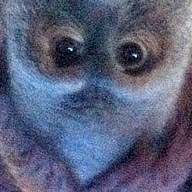
\includegraphics[width=1.5cm]{data/profile.jpg}}
  \vskip 7mm
  \centerline{\begin{minipage}{0.8\textwidth}
  Moje deti sa ma raz spýtali, ako sa programuje. Asi čakali odpoveď na menej ako minútu,
  ja som sa však rozhodol im napísať krátky tutoriál. Krátky tutoriál sa nakoniec trochu 
  rozrástol, zistil som, že to neviem povedať kratšie. Výsledok je tu, poteším sa, ak si ho niekto prečíta. 
    Text aj riešenia úloh sú voľne prístupné
  na Githube na adrese
    \hbox{\href[pdfnewwindow=true]{https://github.com/pocestny/programovanie.git}{https://github.com/pocestny/programovanie.git}}.
  \end{minipage}}
\vfill
v Bratislave \hfill \today
\end{titlingpage}
\hypersetup{pageanchor=true}
\tikzexternalenable




\def\numChapters{40}  
\chapter{Rýchly úvod}
Aby sme mohli rýchlo začať programovať,
spravíme si základnú kostru programu. Čo v nej je si vysvetlíme neskôr, zatiaľ
ju budeme používať bez vysvetlenia:

\begin{lstlisting}
#include <iostream>
using namespace std;
int main() {
  // aj riadok začínajúci sa // je komentár
  // tu bude náš program
}
\end{lstlisting}


Na spustenie sa dá použiť nejaké prostredie (napr.
\link{https://www.codeblocks.org/}{Code::Blocks}, \link{https://visualstudio.microsoft.com}{MS Visual Studio}, ...), alebo linuxový terminál.  V
hocijakom editore (napr. %\link{https://atom.io/}{Atom}
\link{https://bluefish.openoffice.nl/index.html}{Bluefish},
\link{https://kate-editor.org/}{Kate},...) napíš súbor s
programom, ktorý nazvi napr. \vb{program.cc} a skompiluj ho napr. tak, že
v termináli napíšeš \vb{g++ program.cc -o program}. Týmto hovoríš
kompilátoru\footnote{% 
  Kompilátor je program, ktorý z textu programu vyrobí
  spustiteľný kód. V linuxe sú najrozšírenejšie kompilátory \vb{g++} a
  \vb{clang++}. Samozrejme, kompilátor je program, ako každý iný a treba ho mať
  nainštalovaný, aby fungoval.  } 
\vb{g++}, aby zobral program \vb{program.cc}
a vyrobil spustiteľný súbor (binárku) \vb{program}. Potom môžeš spustiť
\vb{./program} Keby program mal chybu, kompilátor vypíše chybovú hlášku a
binárku nevyrobí.  Keby si napríklad namiesto \prg!using! napísal
\prg!fusakla!, chybová hláška by mohla vyzerať nejak takto:

\begin{outputBox}
program.cc:2:1: \textcolor{red}{error:} ‘fusakla’ does not name a type
    2 | \textcolor{red}{fusakla} namespace std;
      | \textcolor{red}{^~~~~~}
\end{outputBox}

Vidíme, že chyba je v súbore \vb{program.cc} na riadku 2 a nasleduje aj opis chyby.
Prostredia ako Code::Blocks chybu zvyčajne vypíšu v samostatnom okne a zvýraznia v texte
programu. Ak je v riadku \vb{//}, zvyšok riadku kompilátor nečíta, môžeš si tam písať poznámky. Ak chceš mať komentár na viac riadkov, dá sa dať medzi 
oddeľovače \vb{/* komentár */}.
Keď už vieš, ako program skompilovať a spustiť, môžeme začať programovať.

\indexItem{Prg}{výraz a príkaz}
Základný stavebný prvok programu je {\em výraz}. Výraz je príklad, ktorý
sa počas behu programu vyráta a zistí sa jeho výsledok ({\em hodnota výrazu}). 
Napr. \prg~3*(2+5)~ je
výraz, ktorého hodnota (výsledok) je \prg~21~.  Druhý stavebný prvok je {\em príkaz}.
Príkaz hovorí, čo sa má s hodnotou výrazu urobiť. 
Príkaz je vždy ukončený bodkočiarkou.  Najjednoduchší
príkaz nerobí nič: \prg~3*(2+5);~ hovorí \cmd{Vypočítaj príklad $3\cdot(2+5)$ a
výsledok zahoď.} \indexItem{Prg}{výpis na \vb{cout} }Príkaz na vypísanie hodnoty na konzolu je \prg~cout<<~ takže
\prg~cout << 3*(2+5);~ znamená \cmd{Vypočítaj príklad $3\cdot(2 + 5)$ a výsledok
vypíš.} Špeciálny výraz je \prg ~endl~, ktorého hodnota je 'koniec riadku'.

Náš prvý program vyzerá takto:

\begin{lstlisting}
#include <iostream>
using namespace std;
int main() {
  cout << 3 * (2 + 5);
  cout << endl;
}
\end{lstlisting}

Keď ho spustíš, vypíše sa \vb{21}.

\indexItem{Prg}{premenná}
\indexItem{Prg}{typ \vb{int}}
Samozrejme nechceme, aby sme pre každý príklad písali samostatný program, ale chceme,
aby jeden program rátal veľa rôznych príkladov. Na to slúžia {\em premenné}. Premenná
je krabička, ktorá má meno a môže v nej byť uložená nejaká hodnota. Každú premennú treba
najprv vyrobiť a pritom treba povedať, aké hodnoty v nej môžu byť uložené (tomu sa hovorí
{\em typ} premennej). Základný typ je \prg~int~. Premenné typu \prg~int~ vedia ukladať celé 
čísla ({\em integer}). Meno typu je zároveň aj príkaz na vyrobenie premennej.
Takže \prg~int x;~ je príkaz, ktorý hovorí \cmd{Vyrob premennú, ktorá sa bude volať 
\prg~x~ a budú sa v nej dať ukladať celé čísla.} Premennú si môžeš nazvať hocijako, ale
meno sa musí skladať z veľkých a malých písmen (bez diakritiky) a podčiarkovníkov (\vb{\_}).
Môžu v ňom byť aj čísla, ale nesmie sa číslom začínať. Napr. \vb{u3\_prachDoma} je
dobré meno premennej. \indexItem{Prg}{priradenie}Príkaz \prg~=~ slúži na uloženie
výsledku do premennej. Takže \prg~x = 3 * (2 + 5);~ hovorí \cmd{Vypočítaj príklad $3\cdot(2+5)$
a výsledok ulož do premennej, ktorá sa volá \prg~x~}. Po vykonaní tohto príkazu
teda v premennej \prg~x~ bude uložená hodnota \prg~21~. Samotné meno premennej
je výraz (t.j. príklad), ktorého hodnota (t.j. výsledok) je číslo, 
ktoré je v nej práve uložené. Čo urobí nasledovný program?

\begin{lstlisting}[label=uvod.1]
#include <iostream>
using namespace std;
int main() {
  int x;
  x = 2 + 5;
  cout << 3 * x; @\ll1@
  cout << endl;
  x = 9 - 5; @\ll2@
  cout << 3 * x; @\ll3@
  cout << endl;
}
\end{lstlisting}

Prvý príkaz na riadku~4 vyrobí premennú \prg~x~, príkaz na riadku~5
vyráta príklad $2+5$ a výsledok (teda $7$)
uloží do premennej \prg~x~. Príkaz na riadku~\ref{uvod.1-1} ráta príklad 
\cmd{Vynásob číslo $3$ a obsah premennej
\prg~x~}. V premennej \prg~x~ je práve uložená sedmička, takže výsledok príkladu je 
$3\cdot7=21$ a to je číslo, ktoré sa vypíše a vzápätí sa vypíše koniec riadku.
Nasledujúci príkaz na riadku~\ref{uvod.1-2} do premennej \prg!x! uloží výsledok príkladu $9-5$, teda $4$. 
Príkaz na riadku~\ref{uvod.1-3} ráta to isté, čo príkaz na riadku~\ref{uvod.1-1}, t.j.
\cmd{Vynásob číslo $3$ a obsah premennej \prg!x!}. Teraz je ale v premennej \prg!x! uložené
číslo $4$, takže výsledok príkladu je $12$.


Posledný príkaz z tejto časti je \indexItem{Prg}{vstup z \vb{cin}}
\prg~cin>>~, ktorý čaká, kým na klávesnici napíšeš číslo (a stlačíš \vb{Enter})
a toto číslo uloží do premennej. Koľko vypíše nasledovný program,
ak mu napíšeš číslo 4? Skús si to najprv vyrátať sám a potom vyskúšať, či si mal pravdu. 

\begin{lstlisting}
#include <iostream>
using namespace std;
int main() {
  int x;
  cin >> x;
  x = x + 5;
  cout << 3 * x;
  cout << endl;
}
\end{lstlisting}

Zopakujme si to. Výraz je príklad, ktorý má výsledok (hodnotu). Videli sme
v ňom vystupovať sčítanie, odčítanie, násobenie, čísla a mená premenných. 
Keď sa počíta výsledok a vo výraze je meno premennej, zoberie sa hodnota, ktorá je v nej 
práve uložená. Toto je dôležité: musíme rozlišovať, medzi tým, čo vieme v čase, keď píšeme 
\indexItem{Alg}{compile-time vs runtime}
program ({\em compile-time}) a tým, čo vie program, keď už pracuje ({\em runtime}).
Napr. ak v predchádzajúcom programe  zadáme číslo 4, vypíše sa $3\cdot(4+5)$, teda $27$.
Ak zadáme číslo $1$, vypíše sa $3\cdot(1+5)$, teda $18$. Pri písaní programu vieme,
že ak napíšeme na vstupe hocijaké číslo $a$, pred výpisom bude v premennej \prg!x! uložená
hodnota $a+5$, a preto sa vypíše  výsledok príkladu $3\cdot(a+5)$.
Nevieme ale dopredu povedať, aké číslo bude v premennej \prg!x! uložené, to bude známe až počas behu programu.

\begin{column}{0.8}
\begin{uloha}
  Máme obdĺžnik z kamienkov ako na obrázku vpravo.
  Napíš program, ktorý prečíta zo vstupu dve čísla: koľko kamienkov je v riadku
  a koľko v stĺpci obdĺžnika. Program má vypísať, koľko kamienkov je v celom obdĺžniku.
  Obrázok vyššie má 5 kamienkov v riadku a 3 riadky a je v ňom  15 kamienkov.
\end{uloha}
\end{column}
\begin{column}{0.2}
  \vspace*{2ex}
  \centerline{
    \begin{tikzpicture}[scale=0.8]
    \foreach \i in {0,...,4} \foreach \j in {0,...,2} {
     \filldraw[fill=brown!90!yellow] (\i*4ex,\j*4ex) circle (1ex);
    }
    \end{tikzpicture}}
\end{column}


\chapter{Podmienky}


Pretože v čase, keď píšeme program, nevieme, čo bude v ktorej premennej uložené,
potrebujeme príkazy, ktoré nám umožnia urobiť rôzne veci, podľa toho, čo sa v premenných
práve nachádza. Predtým si ti ale ešte predstavím iný typ. 
Okrem typu \prg~int~, ktorý znamená celé číslo, 
\indexItem{Prg}{typ \vb{bool}}
je aj typ \prg~bool~ ({\em boolean}), ktorý môže mať dve hodnoty: \prg~true~ (pravda)
a \prg~false~ (nepravda). Rovnako, ako môžeme mať príklady (výrazy) s celými číslami,
môžme mať aj príklady s pravdivostnými hodnotami. Napr. \prg~3 > 5~ je výraz, ktorého
hodnota je \prg~false~. 
\indexItem{Prg}{základné aritmetické a logické operácie}
Tu je niekoľko operácií, ktoré vieme vo výrazoch používať.
Operácie vľavo zoberú dve hodnoty typu \prg!int! a vrátia novú hodnotu \prg!int!.
Mali by byť jasné, len si treba všimnúť, že delenie \prg!/! je vždy celočíselné a zvyšok po 
delení sa dá zistiť pomocou \prg!%!.

V pravej časti sú operácie, ktoré vrátia hodnotu \prg!bool!. Niektoré z nich porovnávajú
čísla typu \prg!int! (\prg!<!, \prg!>!, \prg!<=!,\prg!>=!, \prg!==!, \prg~!=~)
\footnote{Všimni si, že pre porovnanie na rovnosť 
musíme použiť dva znaky \prg!==!, lebo \prg!=! je príkaz 
na uloženie výsledku do premennej} a iné (\prg!&&!, \prg!||!, \prg~!~) kombinujú
hodnoty typu \prg!bool!:\\

\vskip 1ex
  \centerline{
    \begin{tabular}{|c|l||c|l|}\hline
      \multicolumn{2}{|c||}{výsledok je \prg~int~}&
    \multicolumn{2}{c|}{výsledok je \prg~bool~}\\\hline
      \prg~+ - *~& napr. \prg~3 + 2~ & \prg~== > < >= <=~ & napr. \prg~5 >= 3~,  \prg!4 == 4!\\
      \prg~/~ & delenie bezo zvyšku: \prg~7/2~ je \prg~3~& 
      \prg~!=~ & rôzne: \prg~3 != 4~ je \prg~true~\\
      \prg~\%~ & zvyšok po delení: \prg~7 \% 2~ je \prg~1~ &
      \prg~\&\& || ~ & {\em a zároveň}, {\em alebo}\\
      &&\prg~!~&{\em nie}: \prg~!(2==3)~ je \prg!true! \\\hline
    \end{tabular}
  }

  \vskip 1ex  
Pri používaní logických spojok \prg!&&! a \prg!||! má vždy \prg!&&! prednosť pred \prg!||! (podobne ako násobenie 
pred sčítaním), t.j.
\prg!a || b && c! znamená \prg!a || (b && c)!.

\indexItem{Prg}{príkaz \vb{if-else}}
Príkaz \prg~if~ vyhodnotí podmienku (ktorá musí byť napísaná v zátvorkách)
a vykoná iný príkaz iba vtedy, ak výsledok je \prg~true~.
Napr. \prg~if ( x > 5 ) x = 5;~ hovorí \cmd{Zober si hodnotu teraz uloženú v premennej 
\prg~x~ a zisti, či je viac ako 5. Ak je to pravda, 
ulož do \prg~x~ hodnotu 5. Inak neurob nič.} Aby nebolo treba písať veľakrát tú istú 
\indexItem{Prg}{zložený príkaz}
podmienku, existuje tzv. {\em zložený príkaz}. 
Tieto dva programy
sú rovnaké:

\begin{column}{0.45}
\begin{lstlisting}
if (a > 4) x = a;
if (a > 4) x = x + 5;
if (a > 4) cout << x;
\end{lstlisting}
\end{column}
\hfill
\begin{column}{0.45}
\begin{lstlisting}
if (a > 4) {
  x = a;
  x = x + 5;
  cout << x;
}
\end{lstlisting}
\end{column}

Vyrábanie zložených príkazov sa dá použiť kedykoľvek, nielen v príkaze \prg~if~.
Kedykoľvek napíšeme viac príkazov
do kučeravých zátvoriek (\prg~{}~), správajú sa ako jeden príkaz. 
Na každom mieste, kde môžeme použiť príkaz, môžeme 
použiť konštrukciu s kučeravými zátvorkami. Jedným takým miestom je aj začiatok programu.
V našej schéme máme \prg!int main() ! a za ním celý program v kučeravých zátvorkách:
celý program je vlastne jeden zložený príkaz. O vytváraní premenných si viac povieme neskôr,
nateraz skús nevytvárať premenné vovnútri zložených príkazov\footnote{Alebo sa dobre zamysli,
ako sa to asi môže správať.}.

Príkaz \prg~if~ má aj rozšírenú verziu so slovom \prg~else~ (inak):

\begin{lstlisting}
if (a >= 0)
  cout << a;
else
  cout << -a;
\end{lstlisting}

Opäť by sme namiesto každého príkazu mohli použiť zložený príkaz v kučeravých zátvorkách.

Vnáraním podmienok vieme vytvárať rozhodovacie stromy. Povedzme, že máme tri premenné
\prg~a,b,c~ a chceme zistiť, ktorá je najväčšia. To vieme urobiť tak, že sa budeme 
postupne pýtať:\\

\begin{tikzpicture}[xscale=0.9,yscale=1.1]
  \tikzstyle{every node}=[text width=3.2cm,
  draw=brown, thick, fill=yellow!10]
  \tikzstyle{level 1}=[sibling distance=9cm]
  \tikzstyle{level 2}=[sibling distance=4cm]
  \node
  {Platí \prg~a > b~ ?} 
  [level distance =3cm] 
  child{
    node{Ak áno, viem, že \prg~b~ nie je najväčšie, preto 
    najväčšie je \prg~a~ alebo \prg~c~. Stačí mi zistiť, ktoré z nich to je. 
    Opýtam sa, či platí \prg~a > c~.}
    child{node{Ak áno, tak \prg~a~ je najväčšie.}}
    child{node{Ak nie, tak \prg~c~ je najväčšie. }}
  }
  child{
    node{Ak nie, viem, že \prg~a~ nie je najväčšie, preto 
    najväčšie je \prg~b~ alebo \prg~c~. Stačí mi zistiť, ktoré z nich to je. 
    Opýtam sa, či platí \prg~b > c~.}
    child{node{Ak áno, tak \prg~b~ je najväčšie.}}
    child{node{Ak nie, tak \prg~c~ je najväčšie. }}
  }
  ;
  \end{tikzpicture}


Toto viem zapísať do programu :

\begin{lstlisting}
#include <iostream>
using namespace std;
int main() {
    int a, b, c;
    cin >> a >> b >> c;
    if (a > b) {      
      if (a > c)
        cout << a;
      else
        cout << c;
    } else {
      if (b > c)
        cout << b;
      else
        cout << c;
    }
    cout << endl;
}
\end{lstlisting}


Tu som použil skrátený zápis: namiesto \prg~int a; int b; int c;~ môžem napísať
\prg~int a, b, c;~ a namiesto 

\begin{lstlisting}
cin >> a;  cin >> b;  cin >> c;
\end{lstlisting}

môžem písať
\prg~cin >> a >> b >> c;~ Tiež si si už asi všimol, že nezáleží na tom, ako
sú v texte programu medzery a riadky. Je rozumné mať text {\em odsadený} tak,
aby sa dal dobre čítať: každý príkaz na zvláštnom riadku a vnorené príkazy 
majú na začiatku riadku viac medzier, aby začínali viac vpravo. 
Rovnako je dobré nazvať premenné tak,
aby bolo z názvu jasné, čo je v nich uložené. 
Ale nie je to nutné. Aj toto\footnote{
  Program je zo súťaže \href{www.ioccc.org}{\nolinkurl{www.ioccc.org}} o 
  najnečitateľnejší C/C++ 
  program
  (\href{https://www.ioccc.org/2011/eastman/hint.html}{%
\nolinkurl{https://www.ioccc.org/2011/eastman/hint.html}}).}
je správny program, ale nie je ľahké zistiť, 
čo vlastne robí:

\vbox{
\begin{lstlisting}
#include <stdio.h>
#include <math.h>
#include <unistd.h>
#include <sys/ioctl.h>

             main() {
         short a[4];ioctl
      (0,TIOCGWINSZ,&a);int
    b,c,d=*a,e=a[1];float f,g,
  h,i=d/2+d%2+1,j=d/5-1,k=0,l=e/
 2,m=d/4,n=.01*e,o=0,p=.1;while (
printf("\x1b[H\x1B[?25l"),!usleep(
79383)){for (b=c=0;h=2*(m-c)/i,f=-
.3*(g=(l-b)/i)+.954*h,c<d;c+=(b=++
b%e)==0)printf("\x1B[%dm ",g*g>1-h
*h?c>d-j?b<d-c||d-c>e-b?40:100:b<j
||b>e-j?40:g*(g+.6)+.09+h*h<1?100:
 47:((int)(9-k+(.954*g+.3*h)/sqrt
  (1-f*f))+(int)(2+f*2))%2==0?107
    :101);k+=p,m+=o,o=m>d-2*j?
      -.04*d:o+.002*d;n=(l+=
         n)<i||l>e-i?p=-p
             ,-n:n;}}
\end{lstlisting}
}

\begin{uloha}
 Napíš program, ktorý načíta tri čísla a vypíše prostredné z nich.
\end{uloha}

\begin{uloha}
  Napíš program, ktorý načíta číslo mesiaca (1 pre január, 2 pre február, atď.)
  a vypíše číslo ročného obdobia 
  (1 pre jar, 2 pre leto, 3 pre jeseň a 4 pre zimu).
\end{uloha}


\chapter{Cykly}

\indexItem{Prg}{cyklus \vb{while}}
Videli sme už príkazy sa načítanie a vypísanie, uloženie výsledku do premennej
a vyhodnotenie podmienky. Ďalšie užitočné príkazy sú tzv. {\em cykly}, ktoré
nejaký príkaz opakujú viackrát. Predstavíme si jeden z nich: \prg~while~.
Príkaz \prg~while~ má, podobne ako \prg~if~, v zátvorkách napísanú
podmienku a za ňou príkaz. \prg ~while ~robí to, že stále dokola vyhodnocuje
podmienku a kým je splnená, vykonáva príkaz. Podobne ako pri \prg!if!
sa dá použiť zložený príkaz: v \prg!{}! uzavretých viac príkazov
sa správa ako jeden. Čo robí tento program?

\begin{lstlisting}
#include <iostream>
using namespace std;
int main() {
  int x;
  x = 1;
  while (x < 11) {
    cout << x << endl;
    x = x + 1;
  }
}
\end{lstlisting}

Najprv vyrobí premennú \prg~x~ a uloží do nej jednotku. Potom dokola robí toto:
\cmd{Pozri sa, či \prg~x < 11~. Ak áno, vypíš \prg~x~, ulož do \prg~x~ číslo
o 1 väčšie, ako tam bolo doteraz a celé to zopakuj.} Cyklus teda postupne vypíše riadky s 
číslami 1, 2, 3, 4, 5, 6, 7, 8, 9, 10 a potom skončí. Jedna vec, na ktorú si treba dávať pri 
cykle pozor, je, že sa ľahko môže stať, že nikdy neskončí a program sa {\em zacyklí}.
Keby sme napr. zabudli napísať riadok \prg~x = x + 1;~ \prg~x~ sa nikdy nezmení,
\prg~x < 11~ bude platiť stále a program bude donekonečna vypisovať riadok s číslom 1.

Urobme ešte jeden príklad. Dajme tomu, že najprv napíšeš jedno
prirodzené číslo $n$ a potom $n$ prirodzených čísel. Program má zistiť,
ktoré z nich je najväčšie. Napr. ak by si na vstupe napísal \prg!5 6 3 9 12 1!, 
program má vypísať \prg!12!.  Ako to naprogramovať? Najprv si vyrobíme
premennú \prg!int n;! kde si uložíme počet čísel \prg!cin >> n;! Potom
potrebujeme $n$-krát zopakovať toto: \cmd{Prečítaj číslo \prg!x!.  Ak je
väčšie, ako najväčšie číslo, ktoré sme doteraz videli, tak najväčšie videné číslo bude odteraz \prg!x!. Inak sa najväčšie videné číslo nezmení.} 
  Ako
môžme niečo zopakovať $n$-krát? Urobíme cyklus, v ktorom vždy odrátame z
\prg!n!  jednotku.  Keď nám v \prg!n! ostane nula, cyklus skončíme.

\begin{column}{0.6}
Naprogramovať zvyšok už nie je ťažké: budeme mať premennú \prg!int max;!
v ktorej si budeme pamätať doposiaľ najväčšie videné číslo. Vnútri cyklu načítame
jedno číslo zo vstupu a porovnáme ho s \prg!max!. Ostáva vyriešiť jediný problém:
čo dať na začiatku do premennej \prg~max~? A čo sa stane, ak do nej nedáme nič?
  \indexItem{Prg}{nedefinovaná hodnota}
V tom prípade hovoríme, že premenná má {\em nedefinovanú hodnotu} a to znamená, že 
v nej môže byť uložené čokoľvek. Nikdy nepíš program, ktorý používa premennú, do ktorej
predtým nič nezapísal. V našom prípade vieme, že budeš zadávať iba prirodzené čísla.
Keď teda na začiatku do \prg!max! uložíme nejaké záporné číslo, máme istotu,
že už prvé načítané číslo bude väčšie. 
\indexItem{Alg}{zarážka (sentinel)}
Toto je užitočná technika, ktorej sa hovorí 
{\em zarážka} ({\em sentinel}). 
Celý program teda bude vyzerať takto:
\end{column}
\hfill
\begin{column}{0.3}
\vbox{
\begin{lstlisting}
#include <iostream>
using namespace std;
int main() {
  int n, max, x;
  max = -1;
  cin >> n;
  while (n > 0) {
    cin >> x;
    if (x > max) max = x;
    n = n - 1;
  }
  cout << max << endl;
}
\end{lstlisting}
}
\end{column}

\begin{uloha}
  Používateľ napíše najprv jedno prirodzené číslo $n$
a potom $n$ prirodzených čísel. Napíš program, ktorý vypíše ich súčet.
\end{uloha}

\begin{column}{0.7}
\begin{uloha}
  Znova máme kamienky, tentokrát uložené do trojuholníka.
  Napíš program, ktorý prečíta zo vstupu jedno číslo: koľko kamienkov je v 
  spodnom riadku.
  Program má vypísať, koľko kamienkov je v celom trojuholníku. Vieš ho napísať aj bez 
  použitia cyklu?
\end{uloha}
\end{column}
\begin{column}{0.3}
  \centerline{\begin{tikzpicture}
    \foreach \i in {0,...,3} \foreach \j in {0,...,\i}
    \filldraw[fill=brown!90!yellow] (\i*4ex-\j*2ex,\j*4ex) circle (1ex);
  \end{tikzpicture}}
\end{column}

\begin{uloha}
  Napíš program pre takúto úlohu.
  Používateľ postupne zadáva čísla. Keď napíše párne číslo, vypíš to isté číslo.
  Keď napíše nepárne, vypíš o jedno väčšie.
  Keď napíše \vb{-1}, program skončí.
\end{uloha}

\begin{uloha}
  Používateľ najprv zadá číslo $n$ a potom $n$ rôznych čísel. Napíš program, ktorý zistí,
  ako ďaleko sú od seba najväčšie a najmenšie číslo.
\end{uloha}

\begin{uloha}
  Používateľ najprv napíše prirodzené číslo $a$ a potom začne písať
  prirodzené čísla (nevieme, koľko). Nakoniec napíše -1.
  Napíš program, ktorý zistí, koľkokrát je medzi napísanými číslami
  číslo $a$. Napr. pre vstup \prg!3 9 3 8 7 3 6 6 7 3 3 7 8 -1!
  má byť odpoveď \prg!4!, lebo trojka sa v zadaných číslach 
  nachádza štyrikrát.
\end{uloha}

\begin{uloha}
  \label{uloha:collatz}
  Zoberme si takúto hru: mysli si číslo. Ak je párne, vydeľ ho dvoma. Ak je nepárne,
  vynásob ho tromi a pripočítaj 1. Toto opakuj, až kým sa nedostaneš k jednotke.
  Napríklad keď začneš s číslom $12$ budeš postupne dostávať čísla
  $6, 3, 10, 5, 16, 8, 4, 2, 1$.\footnote{V matematike je známa\indexItem{Mat}{Collatzova hypotéza}
  Collatzova hypotéza, ktorá 
  hovorí, že nech začneš z hocijakého čísla, vždy sa nakoniec k jednotke dostaneš.
  Matematikov veľmi hnevá, že stále nevedia Collatzovu hypotézu dokázať.
  Na druhej strane, zatiaľ ani nenašli žiadne číslo, ktoré
  by sa po čase k jednotke nedostalo, a to už vyskúšali všetky čísla až po
  $295147905179352825856$. }

  Napíš program, ktorý prečíta zo vstupu jedno číslo a vypíše, ako dlho trvá, kým
  sa dostaneš k jednotke a aké najväčšie číslo pri tom stretneš. Pre $12$
  má program vypísať $9$ a $16$, lebo k jednote sa dostaneš po $9$ krokoch a 
  najväčšie číslo, ktoré stretneš je 16. Pre $27$ má vypísať $111$ a $9232$.

  (Zistiť, či je číslo párne, sa dá jednoducho pomocou operácie \vb{\%}, ktorá
  dáva zvyšok po delení. Ak teda chceš urobiť nejaký príkaz, iba ak \prg!n!
  je párne, stačí napísať \prg!if (n % 2 == 0) ...!)
\end{uloha}

\begin{uloha} Používateľ postupne zadáva čísla. Napíš program, ktorý
  po každom zadanom čísle vypíše súčet všetkých čísel od začiatku až doteraz.
  Keď používateľ zadá -1, program skončí.
\end{uloha}

\begin{uloha}
  \label{uloha:Fibonacci}
  \indexItem{Mat}{Fibonacciho čísla, zlatý rez}
  Fibonacciho čísla sú postupnosť čísel, ktorú vieme zostrojiť takto: prvé dve
  Fibonacciho čísla sú $0$, $1$. Ďalšie číslo vyrobím tak, že sčítam dve posledné.
  Celá postupnosť teda vyzerá $0,1,1,2,3,5,8,13,21,\ldots$.\footnote{%
   Fibonacciho čísla sú veľmi zaujímavé. Pomer dvoch za sebou idúcich Fibonacciho
   čísel sa blíži k
   tzv. {\em zlatému rezu}. V prírode sa často vyskytujú v rôznych útvaroch, 
   napr. pri špirálach:\newline\newline

    \begin{tikzpicture}[scale=0.15]
      \filldraw[fill=yellow!30!white] (0,0) rectangle node[anchor=center] {$21\times 21$} (21,21);
      \filldraw[fill=green!20!white] (21,21) rectangle node[anchor=center] {$13\times 13$} (34,8);
      \filldraw[fill=red!20!white] (26,8) rectangle node[anchor=center] {$8\times 8$} (34,0);
      \filldraw[fill=blue!20!white] (21,5) rectangle node[anchor=center] {$5\times 5$} (26,0);
      \filldraw[fill=orange!20!white] (21,8) rectangle  (24,5);
      \filldraw[fill=cyan!20!white] (24,8) rectangle  (26,6);
      \filldraw[fill=white] (24,6) rectangle  (25,5);

      \draw[thick,blue] (0,0) 
        arc[start angle=180, end angle=90, radius=21] 
        arc[start angle=90, end angle=0, radius=13] 
        arc[start angle=0, end angle=-90, radius=8] 
        arc[start angle=-90, end angle=-180, radius=5] 
        arc[start angle=180, end angle=90, radius=3] 
        arc[start angle=90, end angle=0, radius=2] 
        arc[start angle=0, end angle=-180, radius=1] 
;
    \end{tikzpicture}
    }
    Napíš program, ktorý pre zadané $n$ vyráta $n$-té Fibonacciho číslo.

\end{uloha}

\indexItem{Alg}{vnorené cykly}
Podobne ako podmienky, aj cykly môžu byť vnorené: príkaz, ktorý sa vykonáva v cykle,
môže opäť obsahovať cyklus. Pozrime na na takýto príklad: používateľ na vstupe napíše číslo
$n$. Program má vypísať šachovnicový vzor rozmerov $n\times n$, pričom sa v ňom
striedavo opakujú \prg!0!
a \prg!1!. Napríklad pre vstup \prg!5! by program vypísal

\begin{outputBox}
01010
10101
01010
10101
01010
\end{outputBox}

Ako naprogramovať niečo takéto? Začiatok je ľahký: budeme mať premennú \prg!int r!, v ktorej
vždy bude uložené, ktorý riadok robíme. Začneme tým, že do nej uložíme nulu a v cykle
ju budeme postupne zväčšovať až po $n-1$. V rámci cyklu potrebujeme vypísať jeden riadok.
Riadok sa skladá z $n$ znakov, preto môžeme použiť inú premennú, \prg!int s!, v ktorej 
bude uložené, ktorý stĺpec v riadku práve robíme. Na začiatku riadku uložíme do
\prg!s! nulu a v cykle budeme $n$-krát pripočítavať jednotku 
a budeme striedavo vypisovať nulu
a jednotku. Vystriedame ich ľahko: ak \prg!x! je 0, tak \prg!1-x! je 1 a naopak.
Posledná otázka: ako zistíme prvý znak v riadku? Premenná \prg!r! udáva číslo riadku
(začína od 0), takže stačí na začiatku zobrať zvyšok po delení 2. Celý program vyzerá takto:\\

\vbox{
\begin{lstlisting}
#include <iostream>
using namespace std;
int main() {
  int r, s, x, n;
  cin >> n;
  r = 0;
  while (r < n) {    // tento cykus sa zopakuje raz pre každý riadok
    x = r % 2;       // x je začiatočný znak
    s = 0;           
    while (s < n) {  // tento cyklus vypisuje znaky v riadku
      cout << x;
      x = 1 - x;     // zmení vypisovaný znak
      s = s + 1;
    }                // koniec cyklu pre znaky v riadku
    cout << endl;    
    r = r + 1;
  }                  // koniec cyklu pre riadky
}
\end{lstlisting}
}

\begin{column}{0.5}
\begin{uloha}
  Napíš program, ktorý načíta jedno číslo $n$ a vypíše štvorec z núl 
  orámovaný jednotkami, ktorý má $n$ riadkov. Pre $n=5$ má vzor vyzerať takto:
\end{uloha}
\end{column}
\hfill
\begin{column}{0.2}
\vspace*{-2ex}
\begin{outputBox}
11111
10001
10001
10001
11111
\end{outputBox}
\end{column}

\begin{column}{0.5}
\begin{uloha}
  Napíš program, ktorý načíta jedno číslo $n$ a vypíše obdĺžnik z núl 
  a jednotiek, ktorý má $n$ stĺpcov a $n+1$ riadkov. Pre $n=5$ má vzor vyzerať takto:
\end{uloha}
\end{column}
\hfill
\begin{column}{0.2}
\vspace*{-2ex}
\begin{outputBox}
00000
00001
00011
00111
01111
11111
\end{outputBox}
\end{column}

\begin{column}{0.5}
\begin{uloha}
  Napíš program, ktorý načíta jedno číslo $n$ a vypíše trojuholníkový vzor z núl 
  a jednotiek, ktorý má $n$ riadkov. Pre $n=5$ má vzor vyzerať takto:
\end{uloha}
\end{column}
\hfill
\begin{column}{0.2}
\vspace*{-2ex}
\begin{outputBox}
000010000
000111000
001111100
011111110
111111111
\end{outputBox}
\end{column}

\chapter{Polia}

Chceme napísať takýto program: najprv napíšeš číslo $n$ a potom $n$ prirodzených 
čísel. Nakoniec napíšeš ešte jedno číslo $a$. Program má vypísať najmenšie zo zadaných čísel,
ktoré je väčšie ako $a$ (alebo vypíše $a$, ak žiadne z čísel nie je väčšie). 
Napríklad:

\vspace*{-2ex}
\begin{column}{0.45}
Vstup\\
\begin{outputBox}
5
1 10 100 1000 10000
427
\end{outputBox}
\end{column}
\hfill
\begin{column}{0.45}
Výstup\\
\begin{outputBox}
1000
\end{outputBox}
\end{column}


Problém je v tom, že keď načítavame čísla zo vstupu, ešte nevieme, ako ich bude treba 
spracovať, takže by sme si ich potrebovali uložiť do premenných. Keby sme počet čísel
poznali v čase písania programu (napr. by bolo povedané, že vždy bude presne päť čísel),
mohli by sme si vyrobiť premennú pre každé číslo. Počet čísel je ale známy až počas behu 
programu. 
\indexItem{Prg}{pole}
Použijeme preto {\em pole} premenných. Pole je vlastne veľa premenných, ktoré
majú spoločné meno a rozlišujú sa číslom (tzv. {\em indexom}). Pole sa vyrobí podobne,
ako jedna premenná, ale v hranatých zátvorkách je uvedený počet premenných.
Tak napr. \prg!int x[10];! vyrobí pole premenných \prg!x[0]!, \prg!x[1]!, až
\prg!x[9]!, z ktorých každá vie mať uložené celé číslo\footnote{Všimni si, že prvá premenná
má číslo 0, preto ak vyrobíme 10 premenných, posledná má číslo 9.}.
Výhoda je, že keď chceme použiť nejakú premennú z poľa, nemusíme písať jej meno priamo,
napr. \prg!x[5]!, ale na mieste indexu môžeme použiť hocijaký výraz. Takže môžeme
napísať \prg!x[2+3]! a tiež dostaneme hodnotu z premennej \prg!x[5]!. A samozrejme,
výraz môže obsahovať aj mená premenných, takže \prg!x[i+3]! znamená \cmd{Pozri sa,
čo je práve teraz uložené v premennej \prg!i!, pripočítaj k tomu 3, výsledok zober ako
číslo premennej z poľa a vráť hodnotu, ktorá je v nej uložená.} Ak by v \prg!i! bola uložená dvojka, tak \prg!x[i+3]! vráti hodnotu
uloženú v premennej \prg!x[5]!. 
Pole nie je premenná, ale veľa premenných. Preto aj príkaz priradenia funguje
na jednotlivých premenných, ale nie na celom poli. Ak by sme mali premenné
\prg!int a[10], b, c[10], d;! môžeme napísať \prg!b=d;! aj \prg!a[d+3]=b;! aj
\prg!c[b+a[d]]=a[d]+c[3];! ale nemôžeme napísať \prg!a=c;! a už vôbec nie
\prg!a=b;! Rovnako, keďže pole nie je premenná, tak nemôžeme používať ani
operácie ako \prg!a+c! alebo \prg!a==c!, ale musíme ich robiť na jednotlivých premenných 
poľa.

Predpokladajme, že máme pole \prg!int a[10];! a premennú \prg!int x!. Čo spraví príkaz
\prg!x=a[22]!? Kompilátor by mal hádam vyhlásiť chybu, ale on nie. 
Premenné sú totiž krabičky, ktoré sú v pamäti uložené jedna za druhou.
Príkazom \prg!int a[10];! kompilátor
vyhradí v pamäti miesto na 10 premenných typu \prg!int! a zapamätá si, kde je prvá z nich,
\prg!a[0]!. Ich počet sa nikde nezapamätá.
Keď napíšeš \prg!a[5]!, znamená to \cmd{piata premenná typu \vb{int} za premennou \prg!a[0]!}. Ak napíšeš
\prg!a[22]!, program sa pozrie do pamäte, kde by bola 23. premenná z poľa, keby to 
pole bolo dosť dlhé. Ak je kratšie, môže na tom mieste byť hocičo (napríklad nejaká
iná premenná) a program sa
začne správať veľmi podivne. Chyby tohto typu sa v programe veľmi ťažko hľadajú.
Preto je dobré dávať veľký pozor, na aké miesta poľa pristupuješ.

\indexItem{Prg}{lenivé vyhodnocovanie podmienok}
Pri pristupovaní do poľa je príjemné, že výrazy typu \prg!bool! sa vyhodnocujú len dovtedy, kým
nie je jasný výsledok, potom sa s počítaním prestane. Napr. pri výraze
\prg!false  && ( zlozita_vec )! je hneď po vyhodnotení prvého \prg!false! jasné, že výsledok bude
\prg!false!, preto sa \prg!zlozita_vec! ani nevykoná. To umožňuje napísať do jednej podmienky 
kontrolu, či je index do poľa správny.
Napr. napíšem
\prg!if (i>=0 && i<10 && a[i]==5)! a viem, že z poľa sa bude čítať iba vtedy, ak je premenná
\prg!i! zo správneho rozsahu.

Vráťme sa k nášmu príkladu. S pomocou poľa a cyklu si vieme zapamätať všetky zadané čísla:

\vskip 2ex
\vbox{
\begin{lstlisting} 
int i, n;
cin >> n;       // prečítam počet čísel 
int x[n];       // vyrobíme pole potrebnej veľkosti
i = 0;         
while (i < n) { // v cykle prečítame všetky prvky poľa
  cin >> x[i];
  i = i + 1;
}
\end{lstlisting}
}

Keď už budeme mať všetky čísla uložené v poli, prečítame zo vstupu číslo $a$. Ak chceme
zistiť najmenšie číslo, ktoré je väčšie ako $a$, urobíme si ďalšiu premennú \prg!min!,
v ktorej si budeme pamätať doteraz nájdené číslo. V cykle sa pozrieme na každú premennú z 
poľa a zistíme, či je jej hodnota väčšia ako $a$. Ak áno a je zároveň menšia ako
\prg!min!, aktualizujeme \prg!min!. Posledná vec: na začiatku potrebujeme do \prg!min!
dať vhodnú zarážku. Môžeme použiť najväčšie číslo, ktoré si môžeme zistiť priebežne
pri ukladaní vstupného poľa. Celý program by vyzeral takto:\\

\vbox{
\begin{lstlisting}
#include <iostream>
using namespace std;
int main() {
  int n, i, a, min;
  cin >> n;
  int x[n];       // vyrobíme pole správnej dĺžky        
  i = 0;
  min = 0;
  while (i < n) { // načítavame vstup a zároveň počítame maximum do zarážky
    cin >> x[i];
    if (x[i] > min) min = x[i];
    i = i + 1;
  }
  cin >> a;       // prečítame a
  i = 0;
  while (i < n) { // v cykle nájdeme hľadané číslo
    if (x[i] > a && x[i] < min) min = x[i];
    i = i + 1;
  }
  cout << min << endl;
}
\end{lstlisting}
}

\begin{uloha}
  Používateľ zadá číslo $n$, potom $n$ čísel a nakoniec číslo $a$. Napíš
  program, ktorý zistí, koľkokrát bolo zadané číslo $a$. Napríklad

\begin{column}{0.45}
Vstup\\
\begin{outputBox}
9 3 9 3 1 3 2 3 4 5 3
\end{outputBox}
\end{column}
\hfill
\begin{column}{0.45}
Výstup\\
\begin{outputBox}
4
\end{outputBox}
\end{column}
\end{uloha}

\begin{uloha}
  Používateľ zadá číslo $n$, potom $n$ čísel a nakoniec číslo $a$. Napíš
  program, ktorý vypíše všetkých $n$ čísel, ale zväčšených o $a$.
\end{uloha}

\begin{uloha}
   Používateľ zadá číslo $n$ a potom zoznam $n$ kariet s číslami. 
   Dvaja hráči, $A$ a $B$ hrajú takúto hru. V každom kole sa $A$ pozrie
   na prvú kartu a $B$ na poslednú kartu (ak je v zozname iba jedna karta,
   je zároveň prvá aj posledná; ak je zoznam prázdny, hra sa skončila).
   Ak $A$ vidí väčšie číslo, výsledok kola je $1$ a $B$ zahodí kartu z konca, 
   ak $A$ vidí menšie číslo, výsledok
   je $-1$ a $A$ zahodí kartu zo začiatku, a ak vidia rovnaké, výsledok je $0$
   a zahodí sa karta z konca aj zo začiatku.
   Napíš program, ktorý prečíta začiatočný zoznam a vypíše postupne výsledky
   všetkých kôl. Napr. pre $n=3$ a vstup \vb{1 2 3} sú výsledky
   kôl \vb{-1 -1 0}.
\end{uloha}

\begin{uloha}
  \label{uloha:sort1}
  Používateľ zadá číslo $n$ a potom $n$ rôznych čísel. Napíš program, ktorý
  najprv vypíše najmenšie číslo a potom vždy najmenšie číslo, ktoré
  je väčšie, ako posledné vypísané. (Všimni si, že program vlastne
  vypíše všetky zadané čísla v utriedenom poradí.)
\end{uloha}

\begin{uloha}
  Používateľ zadá číslo $n$ a potom pole $n$ prirodzených čísel. Napíš program,
  ktorý zistí najväčšie také číslo $k$, že sa v poli nachádza aspoň $k$
  čísel veľkosti aspoň $k$. Napr. pre vstup \prg!9 3 9 1 1 2 2 3 4 5! 
  %(prvá deviatka znamená 9 čísel, potom nasleduje pole) 
  je odpoveď \prg!3!, lebo
  sú tam aspoň tri čísla väčšie alebo rovné $3$ (je tam $5$ takých: $3, 9, 3, 4, 5$),
  ale nie sú tam štyri čísla väčšie alebo rovné $4$ (sú tam len tri: $9, 4, 5$).
\end{uloha}


\chapter{Ďalšie cykly}

Poznáme už príkaz cyklu \prg!while! a úplne by nám stačil, aby sme s ním mohli 
naprogramovať všetko, čo chceme. Sú ale aj ďalšie príkazy cyklov, ktoré môžeme
použiť, aby sme dostali kratší a čitateľnejší program. Veľakrát sme potrebovali
prejsť pomocou cyklu postupne niečo prechádzať. Na to sme vždy mali premennú,
ktorú sme na začiatku nastavili (napr.) na nulu
a v cykle sme ju zvyšovali nejak takto:\\

\begin{lstlisting}
int i;
i = 0;
while (i < n) {
  // niečo urob
  i = i + 1;
}
\end{lstlisting}

Na skrátenie programu a zlepšenie čitateľnosti je možné vyrobenie premennej
a priradenie do nej urobiť naraz, t.j. môžeme napísať\\

\begin{lstlisting} 
int i = 0;
while (i < n) {
  // niečo urob
  i = i + 1;
}
\end{lstlisting}

\indexItem{Prg}{príkaz \vb{for}}
Tento typ programu sa dá čitateľnejšie zapísať iným príkazom cyklu, \prg!for!.
Príkaz \prg!for! má v zátvorkách tri časti, oddelené bodkočiarkami. Prvá časť
je príkaz, ktorý sa má vykonať na začiatku, druhá časť je podmienka ako vo \prg!while!
cykle a tretia časť je príkaz, ktorý sa má vykonať po každom vykonaní cyklu.
Predchádzajúci príklad by mohol vyzerať:\\

\begin{lstlisting}
int i;
for (i = 0; i < n; i = i + 1) {
  // niečo urob
}
\end{lstlisting}


\indexItem{Prg}{inkrement \vb{i++}, \vb{i+=1}}
Rovnako častý je aj príkaz \prg!i = i + 1!, ktorý hovorí \cmd{Zober to, čo je uložené
v premennej \prg!i!, prirátaj 1 a výsledok ulož naspäť do \prg!i!}. Tento príkaz je tak
častý, že má vlastnú skratku, stačí napísať\footnote{\phantomsection\label{foot.inc-vyraz}
  Zvýšenie hodnoty premennej o 1 sa zvykne volať {\em inkrementovanie} a zníženie
  o 1 {\em dekrementovanie}.
  Zápis \vb{i++} sa dá použiť
  aj ako výraz, napr. \vb{ if (i++ < 10) ...} znamená \cmd{Najprv zober hodnotu z premennej \vb{i}.
  Premennú \vb{i} vzápätí zvýš o 1 a pôvodnú hodnotu porovnaj s 10}.
  Podobne sa dá použiť aj \vb{++i}, ktorý inkrementuje premennú pred použitím. 
  Ak je to vo forme príkazu, je to jedno, ale výraz \hbox{\vb{if (++i < 10) ...}} znamená
  \cmd{K premennej \vb{i} najprv prirátaj 1 a potom ju porovnaj s 10}.
  Rovnaký zápis funguje aj pre odčítanie, t.j. \prg!--i! a \prg!i--!.
  Ak chcem pridať inú hodnotu, ako 1, môžem napísať \vb{+=}, napr. \prg!i += 3! namiesto
  \prg!i = i + 3!.
}\prg!i++!. Cyklus tvaru
\prg!for (i = 0; i < n; i++) { ... }! 
je veľmi častý. 

\indexItem{Prg}{príkaz \vb{do-while}}
Príkaz \prg!while! vyhodnocuje podmienku na začiatku, pred vykonaním príkazu. Niekedy
sa viac hodí, aby sa podmienka vyhodnocovala na konci. Na to slúži príkaz 
\hbox{\prg!do!-\prg!while!}. Dajme tomu, že chceme čítať čísla zo vstupu
a vypisovať o jedno väčšie, až kým neprečítame -1. Môžeme to napísať takto:\\

\begin{lstlisting}
int x;
do {
  cin >> x;
  cout << x + 1 << endl;
} while (x >= 0);
\end{lstlisting}

\indexItem{Prg}{príkazy \vb{break}, \vb{continue}}
Niekedy je dobré prerušiť vykonávanie cyklu. Na to slúžia príkazy \prg!break! (skonči
vykonávanie celého cyklu) a \prg!continue! (skonči vykonávanie jednej iterácie a prejdi 
na ďalšiu). Napr. nasledujúci program kopíruje čísla zo vstupu na výstup, 
až kým neprečíta $-1$ a potom skončí:\\

\begin{lstlisting}
while (true) {
  cin >> x;
  if (x == -1) break;
  cout << x << endl;
}
\end{lstlisting}


Podobne nasledujúci program vypisuje iba nepárne čísla, až kým neprečíta -1:\\

\begin{lstlisting}
do {
  cin >> x;
  if (x % 2 == 0) continue;
  cout << x << endl;
} while (x != -1);
\end{lstlisting}


\chapter{Algoritmické úlohy a príkazový riadok}

Všetky úlohy, ktoré si doteraz robil, vyzerali podobne: používateľ niečo napíše na vstupe
(napríklad 7 čísel väčších ako 3),
program s tým má urobiť presne popísanú činnosť (napríklad nájsť najväčšie číslo) a výsledok 
vypísať. Takýmto úlohám, ktoré zo vstupu robia výstup podľa presne stanovených pravidiel
sa hovorí {\em algoritmické úlohy}. Sú dôležité preto, lebo pri nich vieme presne
povedať, kedy je program správny: musí vypísať správny výstup {\em pre všetky} možné vstupy.
Keby sme napr. v úlohe o hľadaní najväčšieho čísla mali program, ktorý skoro vždy
napíše skutočne najväčšie číslo, ale ak je náhodou jedno z čísel na vstupe 12343, 
tak program sa zacyklí,
tak takýto program by bol zlý (aj keby väčšinou fungoval správne).
Aj keď programuješ väčší program, napr. hru, je dobré si ho rozdeliť na menšie, algoritmické,
časti, ktoré sa dajú samostatne skontrolovať. 

Ako sa dajú algoritmické úlohy kontrolovať? Väčšinou nie je možné spustiť program
na všetky možné vstupy, lebo ich je priveľa. Keďže majú presne definované, ako má vyzerať
výstup, je možné o nejakom programe aj matematicky dokázať, že je správny. To býva ale
ťažké, preto sa väčšinou programy {\em testujú}. Snažíme sa vybrať rôzne vstupy a na nich
program spustíme. Keď na všetkých vstupoch dáva správne výsledky, veríme, že je dobrý.
Nájsť dobrú sadu testovacích vstupov býva samo osebe dosť náročné. Je veľa miest,
kde sa dajú algoritmické úlohy trénovať (napr. 
\link{https://testovac.ksp.sk}{testovac.ksp.sk}, \link{https://www.spoj.com}{SPOJ},
%\link{https://codechef.com}{CodeChef}, 
\link{https://codeforces.com}{CodeForces}
a ďalšie). Tieto stránky majú úlohy s možnosťou testovania: odošleš svoj program, na
stránke sa skompiluje, spustí na veľa rôznych vstupoch a oznámi sa ti výsledok. Je aj
veľa súťaží v riešení algoritmických úloh (napr. 
\link{https://www.ksp.sk/}{KSP}, \link{http://oi.sk/}{slovenská} a 
\link{https://ioinformatics.org/}{medzinárodná} olympiáda, \ldots).

\indexItem{Alg}{štandardný vstup/výstup}
Ako si môžeš testovať programy aj sám? Keď program číta vstup pomocou \prg!cin>>! a 
vypisuje na výstup pomocou \prg!cout<<!, používa pri tom tzv. {\em štandardný vstup a výstup}.
Za normálnych okolností je to klávesnica a obrazovka, ale je možné ich 
{\em presmerovať}. Keď v linuxovom termináli spustíš 
\vb{./program <vstup >vystup}, program bude čítať vstup namiesto z klávesnice 
zo súboru \prg!vstup! a vypisovať namiesto obrazovky do súboru \prg!vystup!. Môžeš
si teda napísať rôzne vstupné súbory, ktoré si nazveš napr. \prg!1.in!, \prg!2.in!
atď. a k nim si pripravíš výstupné súbory \prg!1.out!, \prg!2.out! atď so správnymi 
odpoveďami.
Potom môžeš spustiť \vb{./program <1.in >1.prg} a v súbore \vb{1.prg} bude výstup 
programu zo vstupu \vb{1.in}. Teraz stačí porovnať, či sú \vb{1.prg} a \vb{1.out}
rovnaké. To sa dá aj automaticky, pomocou programu \vb{diff}: napíšeš 
\prg!diff 1.prg 1.out!. 
Ak sú rovnaké, 
nevypíše sa nič, inak sa vypíše, kde sa líšia.

Ďalšia možnosť spájania vstupu a výstupu je tzv. {\em pipe}. Ak napíšeš
\prg!./program1 | ./program2! tak sa spustí \vb{program1} a jeho výstup sa použije
ako vstup pre \vb{program2}.  Z príkazového riadku môžeš automaticky spustiť veľa testov.
Príkaz

\vb{for f in *.in; do ./program <\$f | diff - `basename \$f .in`.out; done}

spustí \vb{program} pre všetky súbory s príponou \vb{.in} a pre každý porovná výstup so
súborom \vb{.out} s rovnakým menom. 

Ak zistíš, že v programe je chyba, treba ju hľadať. Prostredia ako \vb{Code::Blocks} umožňujú program
spúšťať príkaz po príkaze a sledovať, ako sa pritom menia hodnoty premenných. To isté vie robiť
aj program, ktorý sa volá {\em debugger}, napr. \vb{gdb}. Pre naše účely ale budú celkom stačiť kontrolné výpisy: na dôležité miesta v programe pridáš vypisovanie premenných a keď spustíš program, vidíš, 
kde sa čo mení. Kontrolné výpisy nakoniec nezabudni vypnúť. Je dobré ich nemazať ale dať do komentárov, 
možno ich ešte v budúcnosti použiješ.

\chapter{Čísla, znaky, reťazce}
\label{sect:cisla}

Doteraz sme hovorili, že typ \prg!int! obsahuje celé čísla. Je to ale trošku zložitejšie.
Skús si napísať takýto program:\\

\begin{lstlisting}
#include <iostream>
using namespace std;
int main() {
  int i, n = 1000;
  for (i = 0; i < 20; i++) {
    cout << n << endl;
    n = 10 * n;
  }
}
\end{lstlisting}


Čo sa deje? Zo začiatku program vypisuje vždy desaťnásobky čísla, tak ako by si čakal:
\vb{1000, 10000, 100000, \ldots}. Po čase sa ale namiesto násobkov desiatky začnú objavovať
čudné čísla. Prečo? Súvisí to s tým, ako sú čísla v počítači uložené. Pamäť sa skladá
zo súčiastok, ktoré môžu byť zapnuté alebo vypnuté, takže celá pamäť počítača sa dá predstaviť
ako véééľmi dlhé pole premenných, z ktorých každá môže byť 0 alebo 1. Takéto premenné
sa volajú {\em bity}. Keď chceme zapísať iné číslo ako 0 alebo 1, musíme ho uložiť
do viacerých bitov. Robíme to pomocou dvojkovej sústavy.

\indexItem{Mat}{dvojková a šestnástková sústava}
Keď zapisujeme čísla, spravidla to robíme v desiatkovej sústave. Pre čísla $0$ až $9$
máme znaky (číslice). Keď potrebujeme zapísať desiatku, na ktorú už nemáme znak, zabalíme
desať jednotiek do jedného balíka a počítame počet balíkov. Číslo $42$ teda znamená 
\cmd{štyri balíky po desať a ešte dve}. Keď sa nám minú číslice pre balíky, začneme
robiť balíky balíkov; počítame stovky a tak ďalej. My to robíme 
po desať, ale to isté môžeme robiť s akýmkoľvek číslom. Keď to budeme robiť s dvojkou\footnote{\phantomsection\label{foot:hexa}%
Často sa používa aj $16$-ková (tzv. hexadecimálna) sústava, kde mám číslice $0,1,2,\ldots,8,9,\mathrm{a,b,c,d,e,f}$, 
takže  \hbox{$\mathrm a_{16}=(10)_{10}$,} \hbox{$\mathrm b_{16}=(11)_{10}$,} \hbox{až $\mathrm f_{16}=(15)_{10}$}
a počítam so základom $16$, napr. $(\mathrm{beef})_{16}=$
\hbox{$\mathrm b_{16}\cdot 16^3+\mathrm e_{16}\cdot16^2+\mathrm e_{16}\cdot16+\mathrm f_{16}=$}
$11\cdot16^3+14\cdot16^2+14\cdot16+15=(48879)_{10}$.
V C++ môžeš priamo písať číslo v $16$-kovej sústave, ak pred neho napíšeš \vb{0x}. Napr. 
\vb{0xff} je \vb{255} a \hbox{\vb{0xfeeddadbeef} je \vb{17518595784431}}.
},
budeme namiesto balíkov po desať robiť balíky po dvoch. Teda budeme počítať $0$, $1$,
potm $10$ (t.j. \cmd{jeden balík po dvoch a nič iné}), $11$, $100$ (t.j. 
\cmd{jeden balík po štyroch a nič iné}), $101$, $110$, $111$ (t.j.
jeden balík po štyroch, jeden balík po dvoch a ešte jedna), $1000$, atď.
Napr. číslo $90$ zapíšeme v dvojkovej sústave $1011010$, pretože
$90=1\cdot64+0\cdot32+1\cdot16+1\cdot8+0\cdot4+1\cdot2+0\cdot1$\\

\centerline{\begin{tikzpicture}
  \foreach \v/\p [count=\i] in { 1/64, 0/32, 1/16, 1/8, 0/4, 1/2, 0/1} {
    \draw[dotted, shorten <= 2ex, shorten >= 2ex] 
    (\i,0) node [color=green!70!black] {{\small \p}}
     -- (\i,-6ex) node {\v};
  }
\end{tikzpicture}}

Názvy premenných sú len vecou programu; v skompilovanej binárke sú inštrukcie pre procesor,
ktoré hovoria, ako sa majú meniť hodnoty na jednotlivých miestach v pamäti.
Miesto v pamäti sa volá {\em adresa}.\indexItem{Alg}{adresa}
Keď v programe napíšeš \prg!int x;! kompilátor si nájde nejaké voľné
miesto v pamäti, kde bude uložená
premenná \prg!x!, zapamätá si jej adresu, a potom 
kedykoľvek v programe napíšeš napr. \prg!x=a!, tak 
kompilátor do 
binárky zapíše
inštrukciu pre procesor, aby počas behu programu nastavil bity
v pamäti na mieste, kde je \prg!x! uložené, podľa dvojkového zápisu $a$. 
Problém je v tom, že rôzne veľké čísla 
majú rôzne dlhý zápis. Keby napr. za premennou \prg!x! mala byť uložená premenná
\prg!y!, jej adresa by sa počas behu programu menila podľa toho, aké veľké číslo
je v premennej \prg!x! práve uložené. To by bolo veľmi nepraktické. Preto sa to rieši tak,
že na každú premennú sa vyhradí fixná dĺžka.
Keby si napísal\\

\vbox{
\begin{lstlisting}[] 
int x = 5591, a[2], r = 6893;
a[0] = 6802;
a[1] = 6737;
\end{lstlisting}
}

a veľkosť \prg!int! by bola
16 bitov, v pamäti by to mohlo vyzerať napr. takto\footnote{%
  Keď sme hovorili o poliach, vravel som, že treba dávať pozor, aby si
  nepísal za koniec poľa. Keby si v tejto situácii napísal \prg!a[2]=55;!,
  prepísala by sa ti premenná \prg!r! a ty by si netušil, kde sa tá chyba nabrala.
  }\\

\centerline{\begin{tikzpicture}[scale=0.2]
  \def\var#1#2#3{%
    \draw[#3] decorate[
       decoration={brace, amplitude=2ex}]{
       (#1,1.8) -- (#1+16,1.8) node [align=center,midway,anchor=south,yshift=2ex] {\vb{#2}}
        };
   \draw[#3,thick] (#1,0) rectangle (#1+16,1.5);

  }
  \foreach \v [count=\i] in {
    0,1,0,0,0,1,0,1,0,1,1,1,0,1,0,1,1,1,0,0,0,1,1,0,1,
    0,1,0,0,1,0,0,1,0,0,0,0,1,1,0,1,0,0,1,0,1,0,0,0,1,
    0,0,0,1,1,0,1,0,1,
    1,1,0,1,1,0,1,0,1
  }{
    \draw (\i,0) rectangle node [anchor=center] {{\scriptsize\roboto \v}} (\i+1,1.5);
  }
  \var3x{blue!50!black}
  \var{19}{a[0]}{red!30!black}
  \var{35}{a[1]}{orange!60!black}
  \var{51}{r}{green!30!black}

  \foreach \x/\v/\a in {3.5/x/142, 19.5/a[0]/158, 35.5/a[1]/174, 51.5/r/190 }{
  \draw[dotted] (\x,-0.1) -- (\x,-3) 
  node[draw, anchor = north west]{\scriptsize adresa \vb{\v} je \a};
  }

\end{tikzpicture}}

Skutočná veľkosť \prg!int! sa líši podľa systému, ale na väčšine súčasných počítačov je to 
32 bitov. Pretože prvý bit je vyhradený na znamienko ($+/-$), najväčšie číslo, aké
si môžeš v premennej typu \prg!int! zapamätať, je $1+2+2^2+2^3+\cdots+2^{30}=2147483647$.
Keby si sa pokúsil ešte pripočítať 1, prvý bit by sa nastavil na 1 a dostal by si záporné 
číslo. 

\indexItem{Prg}{typy \vb{long}, \vb{unsigned}, \vb{char}}
Preto existujú rôzne typy čísel: okrem \prg!int! je \prg!long!, ktorý je spravidla
dvakrát tak dlhý, t.j. má 64 bitov, takže najväčšie číslo je 
$1+2+2^2+\cdots+2^{62}=9223372036854775807$. Oba typy môžeš použiť vo verzii bez
znamienka (\prg!unsigned int!, \prg!unsigned long!) vtedy sa najväčšie číslo zdvojnásobí,
ale nedajú sa pamätať záporné čísla. Vyskúšaj si napísať\\

\vbox{
\begin{lstlisting}[] 
#include <iostream>
using namespace std;
int main() {
  unsigned int x = 0;
  cout << x << endl;
  x = x - 1;
  cout << x << endl;
}
\end{lstlisting}
}

Ako sa dá zapamätať text? Samozrejme, ako čísla. Máme typ \prg!char! (resp. 
\prg!unsigned char!) ktorý je dlhý 8 bitov (t.j. 1 byte). Funguje rovnako ako
typ \prg!int!. Každý znak anglickej abecedy má priradenú číselnú hodnotu podľa 
\indexItem{Alg}{ASCII}
\link{http://www.csc.villanova.edu/~tway/resources/ascii-table.html}{ASCII tabuľky}.
V programe sa dá použiť buď príslušné číslo, alebo znak v apostrofoch.
Keď máš premennú \prg!char x;! tak \prg!x=107;! a \prg!x='k';! urobia to isté.
Keďže je to číslo, dá sa s ním normálne rátať, napr. \prg!'a'+3=='d'! je \prg!true!.

\indexItem{Prg}{string, t.j. reťazec znakov}
Text sa pamätá ako pole znakov, napr. \prg!char hero[8];! Textu, zloženému
zo znakov, sa zvykne hovoriť {\em reťazec} ({\em string}). Príkaz na vypísanie,
\prg!cout<<! za normálnych okolností neakceptuje polia, ale pre pole znakov má výnimku
a vypíše ho ako text. Takisto, zadávať hodnoty \prg!hero[0]=71;! \prg!hero[1]=97;!\ldots
je nepraktické, preto existuje výnimka: pri vyrábaní poľa znakov sa dá priamo
inicializovať textom, napr. \prg!char hero[8]="Gandalf";! vyrobí pole\\

\centerline{\begin{tikzpicture}[scale=0.2]
  \def\var#1#2#3{%
    \draw[#3] decorate[
       decoration={brace, amplitude=2ex}]{
       (#1,1.8) -- (#1+8,1.8) node [align=center,midway,anchor=south,yshift=2ex] {\vb{#2}}
        };
   \draw[#3,thick] (#1,0) rectangle (#1+8,1.5);

  }
  \foreach \v [count=\i] in {
    0,1,
    0,1,0,0,0,1,1,1,
    0,1,1,0,0,0,0,1,
    0,1,1,0,1,1,1,0,
    0,1,1,0,0,1,0,0,
    0,1,1,0,0,0,0,1,
    0,1,1,0,1,1,0,0,
    0,1,1,0,0,1,1,0,
    0,0,0,0,0,0,0,0,
    0,1
  }{
    \draw (\i,0) rectangle node [anchor=center] {{\scriptsize\roboto \v}} (\i+1,1.5);
  }
  \var3G{blue!50!black}
  \var{11}a{red!30!black}
  \var{19}{n}{orange!60!black}
  \var{27}{d}{green!30!black}
  \var{35}a{red!30!black}
  \var{43}l{yellow!50!black}
  \var{51}f{brown!50!black}
  \var{59}{0}{brown!50!black}
  
  \draw[dotted] (3.5,-0.1) -- (3.5,-3) 
  node[draw, anchor = north west]{\scriptsize adresa \vb{hero}};
\end{tikzpicture}}

Je konvencia, že posledný znak reťazca je nula, tak sa ľahko
zabezpečí, že do poľa viem uložiť aj kratší text než
na aký bolo rezervované. 
Len treba myslieť na to, rezervovať pole aspoň
o 1 dlhšie ako najdlhší plánovaný reťazec. 
Pri priradení reťazca do poľa znakov sa dá dľžka poľa vynechať, ak napíšeš
\prg!char hero[]="Gandalf";!, pole \prg!hero! sa vyrobí s dĺžkou $8$.
Pre vypisovanie existuje aj skratka,
že do príkazu \prg!cout<<! sa napíše priamo reťazec v dvojitých úvodzovkách, napr:\\

\vbox{
\begin{lstlisting}[] 
#include <iostream>
using namespace std;
int main() {
  char hero[8] = "Gandalf";
  cout << hero << " is a hero" << endl;
}
\end{lstlisting}
}

Príkaz na vypisovanie vypisuje zaradom 
znaky a skončí, keď narazí na znak 0, takže môže vypísať aj kratšie reťazce.
Čo vypíše tento program?\\

\vbox{
\begin{lstlisting}[] 
#include <iostream>
using namespace std;
int main() {
  char hero[8] = "Gandalf";
  hero[2] = 0;
  cout << "Hero is " << hero << endl;
}
\end{lstlisting}
}

Priradenie do poľa znakov naraz sa dá ale urobiť iba pri jeho vytváraní, takže
napísať neskôr \prg!hero="Batman";! sa nedá.

S načítavaním textu zo vstupu je to podobné, môžeš napísať\\

\vbox{
\begin{lstlisting}[] 
char mojText[20];
cin >> mojText;
\end{lstlisting}
}

Zo vstupu sa začnú čítať znaky až po prvú medzeru, tab, alebo koniec riadku\footnote{%
  \indexItem{Alg}{whitespace}Znaky medzera, tabulátor a nový riadok sa volajú {\em whitespace}.
Toto je dôležité: \prg!cin>>! prestane na prvom whitespace znaku. Aj pri načítavaní
čísel sa whitespace znaky preskakujú, takže je jedno, či sú vstupné čísla oddelené
medzerami alebo koncami riadkov.
Iná je situácia, ak sa načítava typ \prg!char!, vtedy sa whitespace nepreskakuje.
}a budú
sa ukladať do poľa \vb{mojText}. Toto sa ale prudko neodporúča robiť, 
lebo ak je na vstupe viac znakov,
ako je dĺžka poľa, začnú sa prepisovať ďalšie premenné. Vyskúšaj si
písať rôzne vstupy do tohto programu:\\

\vbox{
\begin{lstlisting}[] 
#include <iostream>
using namespace std;
int main() {
  char mojText[5];
  char x = '!';
  cin >> mojText;
  cout << mojText << " " << x << endl;
}
\end{lstlisting}
}


\begin{tabular}{@{\hspace*{0pt}}l@{\hspace*{1cm}}lp{10cm}}
Vstup:&Výstup:\\
\vb{pes} & \vb{pes !} &  nič zvláštne \\
\vb{pes a macka} & \vb{pes !} &  pohoda, načítava sa po prvú medzeru \\
\vb{macka} & \vb{macka } &  znak 0 z konca reťazca prepísal premennú \prg!x!\\
\vb{ABCDEFG} & \vb{ABCDEFG F} &  vypisuje sa až po znak 0, premenná \prg!x!
je prepísaná šiestym znakom
\end{tabular}

Keď na vstupe napíšeš veľmi dlhý text, \indexItem{Alg}{Segmentation fault}
asi spôsobíš, že program skončí s chybou \vb{Segmentation fault}: to je chyba, 
keď sa program snaží písať do takej časti pamäte, kde nemá prístup.
Načítavanie reťazcov je teda lepšie riešiť inak, ale o tom budeme hovoriť neskôr.
Nateraz nám toto stačí.

\begin{uloha}
  Používateľ zadá číslo $n$, potom $n$ čísel.
  Cieľom je vypísať ''súčtovú pyramídu'',
napr.\\

\begin{column}{0.45}
Vstup:\\
\begin{outputBox}
6
1 2 3 4 5 6
\end{outputBox}
\end{column}
\hfill
\begin{column}{0.45}
Výstup:\\
\begin{outputBox}
1 2 3 4 5 6
3 5 7 9 11
8 12 16 20
20 28 36
48 64
112
\end{outputBox}
\end{column}
\end{uloha}


\begin{uloha}
  Na vstupe je najprv číslo $n$, ktoré udáva počet kôp. Potom nasleduje
  niekoľko príkazov. Príkaz sa skladá z kľúčového slova a prípadných parametrov.
  Príkazy môžu byť:

\begin{itemize}\itemsep=-1mm
    \item \textcolor{magenta}{\vb{pridaj} {\em kam koľko}} 
      pridá {\em koľko} na kopu číslo {\em kam}
    \item \textcolor{magenta}{\vb{uber} {\em odkiaľ koľko}}
      uberie {\em koľko} z kopy číslo {\em kam}
    \item \textcolor{magenta}{\vb{max?}}
      zisti, aká veľká je najväčšia kopa
    \item \textcolor{magenta}{\vb{koniec}}
      skonči načítavanie
\end{itemize}

  Napíšte program, ktorý načíta vstup a pri každom príkaze \vb{max?}
  vypíše veľkosť najväčšej kopy. Napr. 

\begin{column}{0.45}
Vstup:\\
\begin{outputBox}
3
pridaj 1 10
uber 1 6
max?
pridaj 2 7
pridaj 2 3
max?
koniec
\end{outputBox}
\end{column}
\hfill
\begin{column}{0.45}
Výstup:\\
\begin{outputBox}
4
10
\end{outputBox}
\end{column}
\end{uloha}

\begin{uloha}
  Na stole sú rôzne geometrické útvary: body, kruhy a úsečky.
  Napíš program, ktorý z opisu predmetov vyráta najmenší obdĺžnik (ktorého
  strany sú rovnobežné s okrajmi stola), v ktorom sú všetky útvary.
  Na začiatku vstupu je počet útvarov $n$, Nasleduje $n$ riadkov,
  každý z nich je jedna z možností

\begin{itemize}\itemsep=-1mm
    \item \textcolor{magenta}{\vb{bod} {\em x y}} 
      bod so súradnicami $[x,y]$
    \item \textcolor{magenta}{\vb{kruh} {\em x y r}}
      kruh so stredom v bode $[x,y]$ a polomerom $r$
    \item \textcolor{magenta}{\vb{usecka} $x_1$ $y_1$ $x_2$ $y_2$}
      úsečka z bodu $[x_1,y_1]$ do bodu $[x_2,y_2]$
\end{itemize}

\begin{column}{0.35}
Vstup:\\
\begin{outputBox}
8
kruh 5 5 3
usecka 1 2 3 4
kruh 7 8 2
kruh 4 3 2
bod 10 5
bod 11 3
usecka 3 3 14 9
kruh 16 5 2
\end{outputBox}

Výstup:\\
\begin{outputBox}
1 1 18 10
\end{outputBox}
\end{column}
\hfill
\begin{column}{0.55}

  \centerline{
  \begin{tikzpicture}[scale=0.45]
    \def\pp{1pt}
    \def\bb(#1,#2){;\filldraw(#1,#2) circle(2pt);}
    \def\cc(#1,#2)#3{\draw(#1,#2) circle (#3);\filldraw(#1,#2) circle(\pp);}
    \def\ll(#1,#2)(#3,#4){
      \draw(#1,#2) -- (#3,#4);
      \filldraw(#1,#2) circle(\pp);
      \filldraw(#3,#4) circle(\pp);
    }
    \draw[step=1.0,black,thin,dotted] (0,0) grid (19,11);
    \foreach \x in {0,...,19} {
      \node at (\x,-0.5) {{\scriptsize $\x$}};
    }
    \foreach \y in {0,...,11} {
      \node[anchor=east] at (0,\y) {{\scriptsize $\y$}};
    }
    \cc(5,5)3
    \ll(1,2)(3,4)
    \cc(7,8)2
    \cc(4,3)2
    \bb(10,5)
    \bb(11,3)
    \ll(3,3)(14,9)
    \cc(16,5)2
    \draw[blue,thick](1,1) rectangle (18,10);
  \end{tikzpicture}}
\end{column}
\end{uloha}

\chapter{Dvojrozmerné polia}
\label{sect:2dpolia}

Po troch vysvetľujúcich kapitolách poďme naspäť k programovaniu. 
Chceme riešiť takúto úlohu: na vstupe sú dve čísla $r$ a $s$ a potom 
tabuľka čísel s $r$ riadkami a $s$ stĺpcami. Úlohou je napísať program, ktorý
tabuľku otočí takto: 

\begin{column}{0.45}
\vbox{
Vstup:\\
\vb{
3 4 \\[1ex]
\begin{tabular}{@{\hspace*{0pt}}cccc}
0&1&2&3\\
  4&5&6&7\\
  8&9&10&11
\end{tabular}
}
}
\end{column}
\hfill
\begin{column}{0.45}
\vbox{
Výstup:\\
\vb{
\begin{tabular}{@{\hspace*{0pt}}ccc}
  0&4&8\\
  1&5&9 \\
  2&6&10\\
  3&7&11
\end{tabular}
}
}
\end{column}


Jeden prístup je prečítať celý vstup do jedného poľa veľkosti $rs$:\\

\vbox{
\begin{lstlisting}[] 
int r, s, i;
cin >> r >> s;
int a[r * s];
for (i = 0; i < r * s; i++) cin >> a[i];
\end{lstlisting}
}

 Fajn, ale ako ho vypísať? Keď si očíslujeme riadky aj stĺpce od 0, tak vidíme,
že číslo v riadku $i$ a stĺpci $j$ bude na pozícii $is+j$:  pred ním je $i$ celých
riadkov po $s$ čísel a ešte $j$ čísel z riadku $i$. Napr. v riadku $2$ a stĺpci $1$ je
číslo $9$:\\


\centerline{\begin{tikzpicture}[scale=0.5]
  \def\row#1#2#3{%
    \draw[#3] decorate[
       decoration={brace, amplitude=2ex}]{
       (#1,1.1) -- (#1+4,1.1) node [align=center,midway,anchor=south,yshift=2ex] {$#2$}
        };
   \draw[#3,thick] (#1,0) rectangle (#1+4,1);
  }
  \foreach \i in {0,...,2} {
    \foreach \j in {0,...,3} {
       \pgfmathtruncatemacro{\v}{\i*4+\j}
       \draw(\j,-\i) rectangle node[anchor=center] {\vb{\v}}  (\j+1,-\i+1) ;
     }
  \draw[teal, -> ] 
    (-1,-1.5) node[anchor=east]{riadok 2} -- (0,-1.5);
  \draw[teal,->]
  (1.5, 2) node[anchor=south]{stĺpec 1} -- (1.5,1);
  \draw[teal,thick] (1,-2) rectangle (2,-1);
    
  \draw[orange] decorate[
       decoration={brace, amplitude=2ex}]{
       (4,-2) -- (0,-2) node [align=center,midway,anchor=north,shift={(0,-0.4)}] {$s$}
        };
 
  \begin{scope}[shift={(8,-2)}]
    \foreach \x in {0,...,11} {
      \draw (\x,0) rectangle node[anchor=center]{\vb{\x}} (\x+1,1);
    }
    \row0{s}{orange}  
    \row4{s}{orange}  
    \draw[teal,thick] (9,0) rectangle (10,1); 
    \draw[teal, ->] (9.5,3) node[black,anchor=south]{$2s+1$} -- (9.5,1);
    \draw (0,0.5) node[anchor=east] {\vb{a:}};
  \end{scope}

}
\end{tikzpicture}}

Vypisovanie vieme urobiť tak, že v jednom cykle (v premennej \prg!j!)
prechádzame po stĺpcoch a pre každý stĺpec ideme v druhom cykle po všetkých
číslach toho stĺpca a vypíšeme ich:\\

\vbox{
\begin{lstlisting}[] 
for (j = 0; j < s; j++) {
  for (i = 0; i < r; i++)
    cout << a[i * s + j] << " ";
  cout << endl;
}
\end{lstlisting}
}

Aby sa nám takéto výpočty zjednodušili, môžeme použiť dvojrozmerné pole, ktoré
vytvorí tabuľku premenných. Príkaz \prg!int a[3][4];! vyrobí premenné\\\indexItem{Prg}{dvojrozmerné pole}


\begin{tikzpicture}[xscale=2,yscale=0.5]
  \foreach \i in {0,...,2}
  \foreach \j in {0,...,3} {
    \draw[draw=none] (\j,-\i) rectangle node [anchor=center]{\vb{a[\i][\j]}} (\j+1,-\i+1);
  }
\end{tikzpicture}

Celý program bude vyzerať takto:\\

\vbox{
\begin{lstlisting}[] 
#include <iostream>
using namespace std;
int main() {
  int r, s, i, j;
  cin >> r >> s;
  int a[r][s];

  for (i = 0; i < r; i++)    // cyklus pre riadky
    for (j = 0; j < s; j++)  // cyklus pre stĺpce
      cin >> a[i][j];

  for (j = 0; j < s; j++) {  // vypíšeme vymenené riadky a stĺpce
    for (i = 0; i < r; i++) 
      cout << a[i][j] << " ";
    cout << endl;
  }
}
\end{lstlisting}
}

\begin{uloha}
  Na vstupe sú čísla $r$, $s$, $d$ a tabuľka čísel s $r$ riadkami a $s$ stĺpcami.
  Napíšte program, ktorý zistí, či sa v tabuľke vyskytuje štvorec $d\times d$
  zo samých núl.
\end{uloha}

\chapter{Čiernobiele obrázky}
\label{sec:CB obrazky}

Dvojrozmerné pole núl a jednotiek sa dá chápať ako čiernobiely obrázok, kde 1 je biela
a 0 čierna. Aby sa dali lepšie pozerať, môžeš si stiahnuť súbor 
\link{\rootpath/obrazok.h}{obrazok.h}, v ktorom som ti
pripravil\footnote{V skutočnosti som len použil program \vb{lodePNG}, ktorý je
voľne prístupný a vie zapisovať obrázky vo formáte PNG.} 
príkaz na zapísanie dvojrozmerného poľa do obrázku. Ukážem ti, ako sa s ním
pracuje. Povedzme, že chceme urobiť obrázok rozmerov $300\times200$, ktorý bude mať
v strede čierny štvorec rozmerov $80\times80$ takto:\\


\centerline{\begin{tikzpicture}[xscale=0.02,yscale=-0.02]
  \def\d{15}
  \def\hl#1{
    \draw[dotted] (-\d,#1) node[anchor=east]{#1} -- (310,#1);
  }
  \def\vl#1{
    \draw[dotted] (#1,-\d)node[anchor=south]{#1} -- (#1,210);
  }
  \draw (0,0) rectangle (300,200);
  \filldraw (110,60) rectangle (190,140);
  \hl0
  \hl{100}
  \hl{200}
  \hl{140}
  \hl{60}
  \vl0
  \vl{300}
  \vl{150}
  \vl{110}
  \vl{190}
\end{tikzpicture}}

Začni tým, že si súbor \vb{obrazok.h} ulož do toho istého adresára, kde máš program
a napíš:\\

\vbox{
\begin{lstlisting}[] 
#include <iostream>
#include "obrazok.h"

int main() {
  int a[200][300], i, j;
  for (i = 0; i < 200; i++)
    for (j = 0; j < 300; j++)
      if (i >= 60 && i <= 140 && j >= 110 && j <= 190)
        a[i][j] = 0;
      else
        a[i][j] = 1;
  zapis_cb_png(200, 300, a, "vystup.png");
}
\end{lstlisting}
}

V druhom riadku hovoríš, že sa má použiť súbor \vb{obrazok.h}. V poslednom riadku
používaš príkaz \hbox{\vb{zapis\_cb\_png},} ktorý je naprogramovaný v tom súbore a má tri parametre, ktoré
sa píšu v zátvorkách:
počet riadkov, počet stĺpcov, dvojrozmerné pole núl a jednotiek a meno výstupného
súboru. Zvyšok by mal byť jasný: premennou \prg!i! prechádzame v cykle cez všetky riadky,
pre každý riadok premennou \prg!j! prechádzame cez všetky stĺpce. 
Pre každé políčko poľa zistíme, aká farba tam má byť, a zapíšeme.
Keď program skompiluješ a spustíš, vyrobí ti súbor \vb{vystup.png}, ktorý
sa dá pozrieť v prehliadači obrázkov.

\begin{uloha}
  Napíš program, ktorý načíta čísla $n$ a $d$ a vyrobí štvorcový obrázok rozmerov 
  $n\times n$ s čiernym rámikom hrúbky $d$.
\end{uloha}

\begin{uloha}
  Napíš program, ktorý prečíta číslo $d$ a spraví obrázok rozmerov $d\times d$
  s čiernym trojuholníkom takto:\\

  
  \centerline{\begin{tikzpicture}[scale=2]
    \draw (0,0) rectangle (1,1);
    \filldraw (0,0) -- (1,1) -- (0,1) -- (0,0);
  \end{tikzpicture}
  }
\end{uloha}


\begin{uloha}
  Napíš program, ktorý prečíta čísla $n$, $d$ a vyrobí obrázok so štvorcovou
  mriežkou $n\times n$ a rozostupmi $d$. Napr. pre $n=301$ a $d=15$ bude obrázok:\\

  
\centerline{
\includegraphics[width=4cm]{data/grid.png}}

\end{uloha}


\begin{uloha}
  Napíš program, ktorý prečíta číslo $d$ a vyrobí obrázok šachovnice ($8\times 8$
  políčok, v ľavom dolnom rohu je čierne políčko) rozmerov $8d\times 8d$, ktorej
  jedno políčko má rozmery $d\times d$.
\end{uloha}


\section*{Malá odbočka: Pytagorova veta, Euklidova vzdialenosť a kruhy}
\label{mat.pytagoras}

\indexItem{Mat}{Pytagorova veta}
Poznáš Pytagorovu vetu? Nie je nová, starí Gréci ju poznali viac ako 300 rokov pr. Kr. 
Asi vieš, že obsah štvorca so stranou $x$ sa dá vypočítať ako $x\cdot x=x^2$.
Pytagorova veta hovorí, že v pravouhlom trojuholníku sa obsah štvorca nad preponou
rovná súčtu obsahov štvorcov nad odvesnami. Alebo kratšie, $c^2=a^2+b^2$:\\


\centerline{
  \begin{tikzpicture}[scale=0.55]
    \filldraw[fill=yellow!20!white] (0,0) -- (4,0) -- (4,3) -- cycle;
    \filldraw[fill=blue!10!white] (0,0) -- (4,0) -- (4,-4) -- (0,-4) -- cycle;
    \filldraw[fill=green!10!white] (4,0) -- (7,0) -- (7,3) -- (4,3) -- cycle;
    \filldraw[fill=red!10!white] (0,0) -- (-3,4) -- (1,7) -- (4,3) -- cycle;
    \draw (2,0) node[anchor = north] {$a$};
    \draw (4,1.5) node [anchor=west] {$b$};
    \draw (2,1.5) node [anchor=south east] {$c$};
    \draw (0.5,3.5) node [anchor=center] {\textcolor{black}{\LARGE $c^2$}};
    \draw (2,-2) node [anchor=center] {\textcolor{black}{\LARGE $a^2$}};
    \draw (5.5,1.5) node [anchor=center] {\textcolor{black}{\LARGE $b^2$}};
  \end{tikzpicture}
}

 Prečo to platí ľahko vidno z nasledujúceho obrázka. 
Vľavo sú štyri rovnaké trojuholníky naukladané do štvorca. 
Pri každom bode v strede strany sú dva rôzne uhly z trojuholníkov,
ktoré dokopy dajú $90^\circ$ (súčet uhlov v trojuholníku je $180^\circ$).
Preto biela vec vovnútri je štvorec.
Vo veľkom štvorci sa iba premiestnili
farebné trojuholníky a vznikol obrázok vpravo, takže plocha bielej časti v oboch 
obrázkoch musí byť rovnaká:


\centerline{\begin{tikzpicture}[scale=0.55]
  \draw (0,0) rectangle (7,7);
  \filldraw[fill=yellow!50!white] (0,3) -- (0,0) -- (4,0) -- cycle;
  \filldraw[fill=red!50!white] (4,0) -- (7,0) -- (7,4) -- cycle;
  \filldraw[fill=blue!50!white] (7,4) -- (7,7) -- (3,7) -- cycle;
  \filldraw[fill=green!50!white] (3,7) -- (0,7) -- (0,3) -- cycle;
  
  \draw (2,0) node[anchor=north] {$a$};
  \draw (5.5,0) node[anchor=north] {$b$};
  \draw (5,7) node[anchor=south] {$a$};
  \draw (1.5,7) node[anchor=south] {$b$};
  \draw (0,1.5) node[anchor=east]{$b$};
  \draw (7,2) node[anchor=west]{$a$};
  \draw (0,5) node[anchor=east]{$a$};
  \draw (7,5.5) node[anchor=west]{$b$};

  \draw (3.5,3.5) node[anchor=center]{{\LARGE $c^2$}};

  \begin{scope}[shift={(12,0)}]
    \draw (0,0) rectangle (7,7);
    \filldraw[fill=green!50!white] (3,7) -- (0,7) -- (0,3) -- cycle;
    \filldraw[fill=red!50!white] (0,3) -- (3,3) -- (3,7) -- cycle;
    \filldraw[fill=yellow!50!white] (3,3) -- (3,0) -- (7,0) -- cycle;
    \filldraw[fill=blue!50!white] (7,0) -- (7,3) -- (3,3) -- cycle;
  
    \draw (0,1.5) node[anchor=east]{$b$};
    \draw (0,5) node[anchor=east]{$a$};
    \draw (5,7) node[anchor=south] {$a$};
  \draw (1.5,7) node[anchor=south] {$b$};
    \draw (7,1.5) node[anchor=west]{$b$};
    \draw (7,5) node[anchor=west]{$a$};
    \draw (5,0) node[anchor=north] {$a$};
  \draw (1.5,0) node[anchor=north] {$b$};
    \draw (1.5,1.5) node[anchor=center]{{\LARGE $b^2$}};
    \draw (5,5) node[anchor=center]{{\LARGE $a^2$}};

  \end{scope}
  
\end{tikzpicture}\\
}

Pytagorova veta zároveň hovorí\footnote{%
  keďže $c^2=a^2+b^2$, tak $c=\sqrt{a^2+b^2}$. \indexItem{Mat}{odmocnina}Znak $\sqrt{x}$ sa číta \cmd{odmocnina
  z $x$} a znamená \cmd{číslo, ktoré keď umocním na druhú (t.j. vynásobím samé so sebou)
  dostanem $x$}, t.j $(\sqrt{x})^2=\sqrt{x}\cdot\sqrt{x}=x$. Napríklad $\sqrt{36}=6$.
  }, že ak mám v rovine dva body, bod $A$ so súradnicami
$[x_1,y_1]$ a bod $B$ so súradnicami $[x_2,y_2]$, tak ich vzdialenosť je \indexItem{Mat}{vzdialenosť bodov}
$\sqrt{(x_2-x_1)^2+(y_2-y_1)^2}$:\\


\centerline{\begin{tikzpicture}[scale=0.8]
  \filldraw (0,0) circle (1pt) node[anchor=east] {$A=[x_1,y_1]$};
  \filldraw (4,3) circle (1pt) node[anchor=south west] {$B=[x_2,y_2]$};
  \draw(0,0)--(4,3);
  \draw[dotted] (0,0) -- (4,0) -- (4,3);
    
    \draw[blue] decorate[
       decoration={brace, amplitude=2ex}]{
       (4,0) -- (0,0) node [align=center,midway,anchor=south,shift={(0,-0.8)}] {$x_2-x_1$}
        };
    \draw[red] decorate[
       decoration={brace, amplitude=2ex}]{
       (4,3) -- (4,0) node [align=center,midway,anchor=west,xshift=2ex] {$y_2-y_1$}
        };
\end{tikzpicture}}


No a napokon kruh so stredom v bode $S=[x,y]$ a polomerom $r$ je tvorený bodmi
$X=[x',y']$, pre ktoré vzdialenosť od $S$ je nanajvýš $r$, takže platí
$(x-x')^2+(y-y')^2\le r^2$. S týmto už ľahko vyriešiš túto úlohu:

\begin{uloha}
  \label{uloha:kruh}
Na vstupe sú čísla $a$ a $r$. Napíš program, ktorý vyrobí obrázok 
rozmerov $a\times a$, ktorý bude mať v strede kruh s polomerom $r$.
Napr. pre $a=300$, $r=100$ bude obrázok vyzerať takto:\\

  {
  \setlength{\fboxsep}{0pt}
\centerline{\fbox{
\includegraphics[width=3cm]{data/kruh.png}}}
  }

\end{uloha}

\section*{Projekt: Celulárny automat}
\label{projekt.automat}

Máme kolóniu baktérií, ktoré žijú na čiare. 
Na začiatku je živá iba jedna baktéria:

\centerline{\vb{..........*..........}}


V každej ďalšej generácii sa kolónia vyvíja podľa nasledovných pravidiel: 
\begin{enumerate}\itemsep=-1mm
    \item ak je na políčku baktéria, ktorá má dvoch susedov, tak skape, lebo nemá dosť miesta
    \item ak je prázdne políčko, ktoré nesusedí s baktériou, ostane prázdne
    \item vo všetkých ostatných prípadoch na políčku bude baktéria
\end{enumerate}

Prvé štyri generácie budú vyzerať takto:

\centerline{\vb{0: ..........*..........}}
\centerline{\vb{1: .........***.........}}
\centerline{\vb{2: ........**.**........}}
\centerline{\vb{3: .......*******.......}}
\centerline{\vb{4: ......**.....**......}}

\begin{uloha}
Napíš program, ktorý načíta $n$ a $t$, pričom $t<n$ a vypíše jeden riadok dĺžky $2n+1$
z bodiek a hviezdičiek, ktorý
bude znázorňovať, ako bude kolónia vyzerať po $t$ generáciách.
\end{uloha}

\begin{uloha}
  Napíš program, ktorý prečíta $t$ a vykreslí obrázok rozmerov $(2t+1)\times t$, v ktorom
  $i$-ty riadok bude zodpovedať $i$-tej generácii: ak je na políčku baktéria, bude tam 
  čierny pixel,
  inak biely. Prvý riadok bude celý biely, iba v strede (na pozícii $[0][t]$) bude
  čierny pixel.
\end{uloha}

 Môžeme ďalej skúmať, ako by vyzeral náš obrázok, keby kolónia mala iné pravidlá.
Políčko má  osem možností, ako môže vyzerať jeho okolie:


\centerline{\begin{tikzpicture}[scale=0.3]
  \def\n#1#2{
    \filldraw[fill=\if#10white\else black!30!white\fi] (#2,0) rectangle (#2+1,1);
  }
  \def\N#1#2#3#4{
    \draw(1.5,1.5) node[anchor=south] {$#4$};
    \n#10\n#21\n#32
  }
  
  \foreach \v [count = \i] in {0000,0011,0102,0113,1004,1015,1106,1117} {
    \begin{scope}[shift={(-4*\i,0)}]
      \expandafter\N\v
    \end{scope}
  }
\end{tikzpicture}}


Ak si všimneš, očísloval som ich tak, že ak plné políčko je jednotka a prázdne políčko je 
nula, tak políčka vlastne tvoria číslo okolia zapísané v dvojkovej sústave, napr. okolie
s číslom 5 je
\vb{101}. Inak povedané, ak mám tri čísla (nuly a jednotky) 
$x,y,z$, tak číslo okolia je $4x+2y+z$.


Pravidlo pre rast kolónie musí pre každé okolie povedať, či v ňom v ďalšej generácii
bude baktéria alebo nie. Naše pravidlo vyzerá takto:


\centerline{\begin{tikzpicture}[scale=0.3]
  \def\n#1#2{
    \filldraw[fill=\if#10white\else black!30!white\fi] (#2,0) rectangle (#2+1,1);
  }
  \def\N#1#2#3#4#5{
    \draw(1.5,1.5) node[anchor=south] {$#4$};
    \n#10\n#21\n#32
    \begin{scope}[shift={(1,-1)}]\n#50\end{scope}
  }
  
  \foreach \v [count = \i] in {00000,00111,01021,01131,10041,10151,11061,11170} {
    \begin{scope}[shift={(-4*\i,0)}]
      \expandafter\N\v
    \end{scope}
  }
\end{tikzpicture}}


Každé pravidlo viem opísať pomocou 8 núl alebo jednotiek, ktoré hovoria výsledok pre 
jednotlivé okolia. Naše pravidlo je \vb{01111110}. Keď si predstavíme, 
že to je zápis nejakého čísla v dvojkovej sústave, každé z 256 možných
pravidiel kolónie môžeme označiť číslom z rozsahu $0$ až $255$.
Naše pravidlo je


\centerline{\begin{tikzpicture}
  \foreach \v/\p [count=\i] in { 0/128, 1/64, 1/32, 1/16, 1/8, 1/4, 1/2, 0/1} {
    \draw[dotted, shorten <= 2ex, shorten >= 2ex] 
    (\i,0) node [color=green!70!black] {{\small \p}}
     -- (\i,-6ex) node {\v};
  }
\end{tikzpicture}}

\indexItem{Prg}{bitové operácie}
$64+32+16+8+4+2=126$. Našim cieľom teraz bude preskúmať rôzne pravidlá.
Ako ľahko pracovať s číslom pravidla? Na to pomôžu tzv. {\em bitové operácie}. Sú to
operácie nad celými číslami (podobne ako \vb{+,-,*,/,\%}), ale pracujú s jednotlivými
bitmi čísla v dvojkovej sústave.\\

\def\prikl#1#2#3{\raisebox{-1.5cm}{%
  \begin{tikzpicture}[scale=0.45]
    \def\p(##1,##2)##3{\draw[draw=none] (##1,##2) 
    rectangle node[align=center]{\vb{##3}} (##1+1,##2+1);
    }
    \foreach \x[count=\i] in {8, 4, 2, 1}{
      \draw[draw=none] (\i,1) rectangle node[color=green!60!black, align=center]
      {{\scriptsize\roboto \x}} (\i+1,2);
    }
    \p(0,0){#1:}
    \foreach \x [count=\i] in \opA {\p(\i,0){\x}}
    \p(0,-1){#2:}
    \foreach \x [count=\i] in \opB {\p(\i,-1){\x}}
    \draw (0,-1.2) -- (5,-1.2);
    \p(0,-2.2){#3:}
    \foreach \x [count=\i] in \res {\p(\i,-2.2){\x}}
  \end{tikzpicture}}
}



\centerline{\begin{tabular}{|c|c|p{7cm}|l|p{2.5cm}|}\hline
\vb{\&} & AND & 
  výsledok je číslo, ktoré má bit nastavený na 1, ak obe čísla majú
  príslušný bit 1
  & \vb{10 \& 9 == 8} &
\global\def\opA{1,0,1,0}
\global\def\opB{1,0,0,1}
\global\def\res{1,0,0,0}
  \prikl{10}{9}{8} \\\hline
\vb{|} & OR & 
  výsledok je číslo, ktoré má bit nastavený na 1, ak aspoň jedno číslo má
  príslušný bit 1
  & \vb{10 | 9 == 11} &
\global\def\opA{1,0,1,0}
\global\def\opB{1,0,0,1}
\global\def\res{1,0,1,1}
  \prikl{10}{9}{11} \\\hline
  \vb{\^{}} & XOR & 
  výsledok je číslo, ktoré má bit nastavený na 1, ak práve jedno číslo má
  príslušný bit 1
  & \vb{10 \^{} 9 == 3} &
\global\def\opA{1,0,1,0}
\global\def\opB{1,0,0,1}
\global\def\res{0,0,1,1}
  \prikl{10}{9}{3} \\\hline
\end{tabular}}


Ešte sa hodia dve bitové operácie. Operácia \prg!<<! posúva binárny zápis čísla doľava.
\prg!x << a! pripíše \vb{a} núl na koniec dvojkového\footnote{\phantomsection\label{foot:hexa2}%
Tu sa prejaví výhoda $16$-kovej sústavy. Pretože $16=2^4$, jedna cifra v $16$-kovej sústave priamo
zodpovedá štyrom binárnym cifrám. Takže napr. \vb{0xff<<8} je \vb{255<<8}, t.j. 
$255\cdot2^8=255\cdot256=65280$, čo je \vb{0xff00}. 
}zápisu \vb{x}. To je to isté,
ako keby som ho \vb{a}-krát za sebou vynásobil dvomi. Napr $5$ je v dvojkovej sústave
\vb{101}. \prg!5 << 3! preto bude číslo s dvojkovým zápisom \vb{101000}, čo je
$5\cdot8=40$. Opačná operácia \prg!>>!posúva číslo doprava, t.j. zoberie celú časť po delení dvomi.
Napr. $45$ je v dvojkovej sústave \vb{101101}. Keď ho trikrát vydelím dvomi a vždy zoberiem celú časť, dostanem
\vb{10110} (čo je $22$), \vb{1011} (čo je $11$) a \vb{101} (čo je $5$). Preto \prg!45 >> 3! je $5$. 


S týmito operáciami viem jednoducho vyhodnocovať pravidlá. Predpokladajme, že mám
pravidlo \prg!r! a niekde
v poli mám hodnoty políčok \prg!a[i-1]!, \prg!a[i]!, \prg!a[i+1]!. 
Číslo okolia (od 0 do 7) dostanem tak, že
vyrátam \hbox{\prg!z = 4 * a[i-1] + 2 * a[i] + a[i+1]!}. 
Bit na pozícii \vb{z} v pravidle mi hovorí, či bude políčko v ďalšej generácii 
obsadené. Preto stačí vyrátať \prg!r & (1 << z)!, t.j. jednotku posunúť o \vb{z}
pozícií doprava a urobiť operáciu AND s pravidlom. Ak je výsledok 0, políčko má byť
prázdne. Ak je výsledok nenulový (t.j rovný \prg!1 << z!), na políčku bude baktéria.

\begin{uloha}
  Napíš program, ktorý načíta číslo pravidla $r$ a počet iterácií $t$ a vyrobí obrázok
  (rozmerov $2t+1\times t$),
  ako vyzerá vývoj kolónie s pravidlom $r$ počas $t$ generácií.
\end{uloha}


Môžeš skúmať rôzne pravidlá: niektoré kolónie rýchlo vymrú, niektoré vyrobia jednoduché útvary 
(napr. čiaru), iné robia tzv. deterministický chaos, a ešte iné rôzne pravidelné
obrazce. Niekoľko pravidiel je tu\footnote{Všimni si, že párne pravidlo vytvorí biele pozadie a nepárne pravidlo pásikavé. Je to náhoda? Vieš povedať,
prečo to tak je?}:


\vbox{
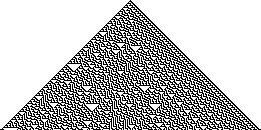
\includegraphics[width=7cm]{data/r86.png}
\hfill
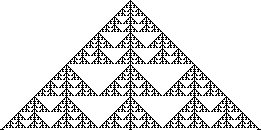
\includegraphics[width=7cm]{data/r150.png}\\
\hbox to 7cm{\hss pravidlo 86\hss}
\hfill
\hbox to 7cm{\hss pravidlo 150\hss}
}

\vskip 1ex

\vbox{
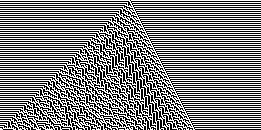
\includegraphics[width=7cm]{data/r89.png}
\hfill

\includegraphics[width=7cm]{data/r107.png}\\
\hbox to 7cm{\hss pravidlo 89\hss}
\hfill
\hbox to 7cm{\hss pravidlo 107\hss}
}


Rovnako dobre sa dá skúšať, čo sa stane, ak kolónia nezačína z jednej baktérie, ale z 
niekoľkých, ako sa správajú dve rastúce kolónie, ktoré do seba narazia, čo ak 
je pravidlo z väčšieho okolia a pod.


\chapter{Funkcie}

Kapitolu~\ref{sec:CB obrazky} som začal tým, že som ti pripravil súbor, v ktorom
bol nový príkaz \prg!zapis_cb_png!. Teraz ti idem ukázať, ako si nové príkazy, ktorým
sa hovorí {\em funkcie}, môžeš vyrobiť aj ty. 
Možnosť vyrobiť si vlastné funkcie je veľmi dôležitá:
umožňuje ti rozdeliť si veľký program na malé časti, ktoré potom môžeš používať viackrát.


Najjednoduchšia funkcia vyzerá takto:\\

\vbox{
\begin{lstlisting}[] 
#include <iostream>
using namespace std;

int sedem() {
  return 7;
}

int main() {
  cout << sedem() << endl;
}
\end{lstlisting}
}

Všimni si, že sa veľmi podobá na zápis, ktorý používame na program. Nie je to náhoda.
Celý program je v skutočnosti len kopa funkcií, ibaže jedna z nich je špeciálna: tá, ktorá
sa volá \prg!main! sa začne vykonávať ako prvá. Každá funkcia je samostatný program,
ktorý má svoj vlastný svet.

 Funkcia má meno\footnote{Podobne
ako pri premenných, meno funkcie môže byť čokoľvek z veľkých a malých písmen, podčiarkovníkov
a čísel, ale nesmie začínať číslom.} a typ. V našom programe sme spravili funkciu, ktorá
sa volá \vb{sedem}. Typ \prg!int! pred jej menom hovorí, že táto funkcia predstavuje
výraz, ktorého výsledok je celé číslo.
Guľaté zátvorky za menom slúžia
na parametre. Zatiaľ žiadne nemáme, ale zátvorky aj tak treba písať, aby bolo jasné, že je to funkcia a nie premenná.
Potom nasleduje zložený príkaz, t.j. v kučeravých zátvorkách napísané príkazy. 

 Funkciu vieme v nejakej inej funkcii použiť ({\em zavolať}) tak, že napíšeme jej meno a parametre,
v našom prípade \prg!sedem()!. 
Pretože naša funkcia má typ \prg!int!, vieme, že každé jej zavolanie {\em vráti} celé číslo a
môžme ju použiť
vo výrazoch rovnako, ako by sme používali číslo. Môžeme napr. urobiť 
\prg!int x = 3 + sedem();! a pod. Kedykoľvek treba vyhodnotiť výraz, v ktorom
sa volá funkcia, všetko sa preruší a spustí sa tá funkcia. Príkaz
\prg!cout << sedem() << endl;! v našom programe hovorí \cmd{
  Začni vypisovať, mal by si vypísať číslo. Preruš robotu, spusti funkciu \prg!sedem()! 
  a počkaj, kým skončí.
Keď skončí, ako výsledok ti dá číslo. Pokračuj vo vypisovaní, vypíš  toto číslo a potom znak 
konca riadku.}

\indexItem{Prg}{\vb{return}}
 Príkazy, ktoré sa vo funkcii vykonávajú sa volajú {\em telo} funkcie. Špeciálny 
príkaz \prg!return vyraz;! urobí to, že skončí funkciu a výsledok funkcie 
(tzv. {\em návratová hodnota}) bude hodnota výrazu \prg!vyraz!. Typ výrazu musí byť rovnaký
ako návratový typ funkcie, ktorý sme zadali pri jej definícii. Napr. naša funkcia
\prg!sedem()! vracia typ \prg!int!, preto výraz v príkaze \prg!return! musí mať hodnotu typu
\prg!int!. Funkcie ale môžu mať ako návratovú hodnotu ľubovoľný typ. Ak by som mal
funkciu \prg!bool zle() { return false; }!, môžem ju použiť všade, kde môžem mať výraz typu
\prg!bool!, napr. \prg!if (zle()) {}!.


Každá funkcia musí skončiť príkazom
\prg!return!\footnote{Slušné by bolo, aby sme aj na konci hlavného programu písali 
\prg!return 0;!, ale keďže už potom program skončí, tak to nevadí, keď to vynecháme.}.
Funkcia je samostatný svet, takže môže mať vlastné premenné. Tie sú úplne nezávislé
od iných funkcií (hovoríme im \indexItem{Prg}{lokálne premenné}{\em lokálne premenné}). Čo urobí tento program?

%\vbox{
\begin{lstlisting}[] 
#include <iostream>
using namespace std;

int pridaj() {
  int x;
  cin >> x;
  return x + 7;
}

int main() {
  int x = pridaj();
  cout << x + pridaj() << endl;
}
\end{lstlisting}
%}

Hlavný program vyrobí premennú \prg!x!. Zavolá funkciu \prg!pridaj()! a jej
výsledok má uložiť do \prg!x!. Keď sa zavolá funkcia \prg!pridaj()!, vznikne 
nový svet, v ktorom sa vytvorí iná premenná \prg!x! a načíta sa do nej číslo zo vstupu.
Dajme tomu, že používateľ napíše 2.
Potom sa funkcia \prg!pridaj()! skončí, jej svet zanikne, a ostane len výsledok, číslo 9. 
Pracovať pokračuje hlavný program, do svojej premennej \prg!x! 
uloží výsledok volania funkcie, t.j. 9. Pokračuje príkazom \prg!cout <<!, 
na to potrebuje vyhodnotiť
výraz \prg!x + pridaj()!. V \prg!x! má 9, opäť preruší robotu a zavolá \prg!pridaj()!.
Zase vznikne nový svet s premennou \prg!x!, do ktorej sa prečíta hodnota. 
Dajme tomu, že teraz
je na vstupe 3. Funkcia skončí, jej svet zanikne a ostane číslo 10. Hlavný program
teraz dokončí rátanie výrazu \prg!9 + 10! a vypíše \prg!19!.


\indexItem{Prg}{parametre funkcie}
Doteraz sme nehovorili o parametroch. Parametre umožňujú používať tú istú funkciu na
rátanie rôznych vecí. Sú to premenné, ktoré sú lokálne premenné funkcie, ale
ich hodnota sa dá nastaviť zvonka pri volaní funkcie. Parametre a ich typy
sú uvedené v zátvorkách za menom funkcie, takže napr.\\

\vbox{
\begin{lstlisting}[] 
int scitaj(int x, int y) {
  int z = x + y;
  return z;
}
\end{lstlisting}
}

je funkcia, ktorá má dva parametre a oba sú celé čísla. Vo vnútri funkcie sa 
k nim dá správať ako k normálnym premenným. Majme hlavný program:\\

\vbox{
\begin{lstlisting}[] 
int main() {
  int x = 1;
  x = scitaj(x, scitaj(x, 3 * x));
  cout << x << endl;
}
\end{lstlisting}
}

Skús sa zamyslieť, čo vypíše. Máš to? Poďme to pozrieť detailne. Hlavný program
sa spustí, vyrobí si svoju premennú \vb{x} a dá do nej $1$. Potom ide
vyhodnocovať výraz, ktorého výsledok má uložiť do \vb{x} a zistí, že je to 
volanie funkcie.

\def\tw{2}
\def\th{3ex}
\def\r{1ex}
\def\vw{3.5ex}
\def\mimo{\color{black!50!white}}
\def\hi{\color{red!50!black}}
\def\dn{\color{blue!80!white}}
\def\fr#1{
  \filldraw[thick,draw=\clr,fill=white,rounded corners=\r] (0,\th) rectangle (\tw,-\r);
  \filldraw[draw=none, fill=white] (0,0) rectangle (\w,-\h);
  \draw[thick,draw=\clr] (0,-\h) -- (0,0) -- (\w,0) -- (\w,-\h);
  \draw[thick,draw=none] (0,\th) rectangle node[color=\clr,anchor=center]{\vb{#1}} (\tw,0);
}
\def\var(#1,#2)#3#4#5{
  \draw (#1,#2) rectangle node[anchor=center]{#4} (#1+\vw,#2-\vw) 
  coordinate[pos=0.5] (#5);
  \node [anchor=east] at (#1,#2-0.5*\vw) {\vb{#3:}};
}

\def\conn[#1][#2](#3,#4){
    \draw[draw=orange, thick, ->, shorten >= 3ex, shorten <= 3ex] (#1) to[in=#3,out=#4] 
    node[midway, above, color=orange]{}(#2);
}

\def\fsc{[yscale=0.78]}
\begin{tikzpicture}\fsc
  \def\h{1.8}
  \def\w{6.2}
  \def\clr{green!55!black}
  \fr{main}
  \var(4ex,-1ex){x}{1}{mX}
  \node [anchor=south west] at (0,-10ex) {\vb{ 
  {\mimo x = {\hi scitaj(}x, scitaj(x, 3 * x){\hi )}};}};
\end{tikzpicture}


Vyrobí sa teda nový svet funkcie \vb{scitaj} a hlavný program chce nastaviť
hodnoty parametrov. 
Prvý parameter nastaví podľa aktuálneho obsahu \vb{x}, 
ale pri druhom zistí, že je to výraz, v ktorom 
je opäť volanie funkcie.


\begin{tikzpicture}\fsc
  \def\h{1.8}
  \def\w{6.2}
  \def\clr{green!55!black}
  \fr{main}
  \var(4ex,-1ex){x}{1}{mX}
  \node [anchor=south west] at (0,-10ex) {\vb{ 
  {\mimo x = {\dn scitaj(x, }{\hi scitaj(}x, 3 * x{\hi )}{\dn )}};}};

  \begin{scope}[shift={(8,-1)}]
  \def\h{1}
  \def\w{4}
  \def\clr{blue!55!black}
  \fr{scitaj}
  \var(4ex,-1ex){x}{1}{vX}  
  \var(15ex,-1ex){y}{}{vY}  
  \draw[draw=\clr](0,-5ex) -- (\w,-5ex); 
  \conn[mX][vX](150,10);
  \end{scope}
\end{tikzpicture}

 Vytvorí sa teda ďalší, nezávislý, svet funkcie \vb{scitaj}, nastavia sa mu hodnoty
parametrov a vyráta sa výsledok, ktorý sa potom vráti tomu, kto funkciu zavolal.


\tikzexternaldisable
\begin{tikzpicture}[remember picture, yscale=0.78]%\fsc
  \def\h{1.8}
  \def\w{6.2}
  \def\clr{green!55!black}
  \fr{main}
  \var(4ex,-1ex){x}{1}{mX}
  \node [anchor=south west] at (0,-10ex) {\vb{ 
  {\mimo x = {\dn scitaj(x, }{\hi scitaj(}x, 3 * x{\hi )}{\dn )}};}};

  \begin{scope}[shift={(10,0.2)}]
  \def\h{1}
  \def\w{4}
  \def\clr{blue!55!black}
  \fr{scitaj}
  \var(4ex,-1ex){x}{1}{vX}  
  \var(15ex,-1ex){y}{}{vY}  
  \draw[draw=\clr](0,-5ex) -- (\w,-5ex); 
  \end{scope}
  
  \begin{scope}[shift={(7.5,-1)}]
  \def\h{2.6}
  \def\w{4}
  \def\clr{orange!55!black}
  \fr{scitaj}
  \var(4ex,-1ex){x}{1}{vvX}  
  \var(15ex,-1ex){y}{3}{vvY}  
  \draw[draw=\clr](0,-5ex) -- (\w,-5ex); 
  \conn[mX][vvX](140,20);
  \conn[mX][vvY](140,20);
  \var(4ex,-6ex){z}{4}{vvZ}  
    \node [anchor=south west] at (0,-13ex) {\vb{... }};
    \node [anchor=south west] at (0,-16ex) {\vb{return z;}};
  \draw[draw=\clr](0,-\h) -- (\w,-\h); 
  \end{scope}
\end{tikzpicture}

 Teraz druhý svet zanikne, ostane z neho iba výsledok $4$, a tým sa nastaví parameter
v prvom svete:


\begin{tikzpicture}[remember picture,  yscale=0.78]
  \def\h{1.8}
  \def\w{6.2}
  \def\clr{green!55!black}
  \fr{main}
  \var(4ex,-1ex){x}{1}{mX}
  \node [anchor=south west] at (0,-10ex) {\vb{ 
  {\mimo x = {\dn scitaj(x, }{\color{white} scitaj(x, 3 * x )}{\dn )}};}};
  \node[anchor=south west] (vys) at (24ex,-10ex) {\color{orange} 4};

  \begin{scope}[shift={(8,-0.5)}]
  \def\h{2.6}
  \def\w{4}
  \def\clr{blue!55!black}
  \fr{scitaj}
  \var(4ex,-1ex){x}{1}{vX}  
  \var(15ex,-1ex){y}{4}{vY}  
  \draw[draw=\clr](0,-5ex) -- (\w,-5ex); 
  \var(4ex,-6ex){z}{5}{vZ}  
    \node [anchor=south west] at (0,-13ex) {\vb{... }};
    \node [anchor=south west] at (0,-16ex) {\vb{return z;}};
  \draw[draw=\clr](0,-\h) -- (\w,-\h); 
  \end{scope}
 
  \conn[vys][vY](150,10);
  %\conn[vvZ][vys](0,0);
    \draw[overlay, draw=orange!80, thick, ->, opacity=0.4, shorten >= 1ex, shorten <= 3ex] (vvZ) to[in=90,out=180] 
    node[midway, above, color=orange]{}(vys);
\end{tikzpicture}
\tikzexternalenable


Napokon zanikne aj prvý svet, ostane hodnota 5 a tá sa zapíše do premennej \vb{x}
v hlavnom programe. Takže si to zhrňme: funkcia je samostatný program, ktorý má 
výstupnú hodnotu\footnote{Tu len pripomeniem: úplne na začiatku sme hovorili,
že najjednoduchší príkaz \vb{3*(2+5);} len vyráta hodnotu $21$ a výsledok zahodí. 
To je, samozrejme, zbytočné, ale niekedy môžeš chcieť zahodiť hodnotu funkcie. Napríklad
ak zoberiem funkciu \vb{pridaj} z predchádzajúceho príkladu , tak
volanie \prg!pridaj();! načíta číslo zo vstupu a 
ignoruje ho.}.
Dá sa použiť vo výrazoch. Pri volaní funkcie sa vytvorí
nový nezávislý svet, nastavia sa hodnoty parametrov\footnote{%
Zatiaľ vieme ako parametre funkciám posielať jednoduché premenné, ale nie polia. 
Polia sa tiež dajú ako parametre použiť, ale o tom až neskôr.
} a vypočíta sa výstupná hodnota.

\begin{uloha}
  Napíš funkciu \vb{max} s tromi parametrami, ktorá vráti najväčší z nich.
\end{uloha}

\begin{uloha}
  Napíš funkciu \prg! int dlzka(int n) {...}!, ktorá pre zadané číslo $n$
  vráti počet cifier (napr. \vb{dlzka(546)} je 3). Pomocou nej napíš program,
  ktorý prečíta zo vstupu číslo \vb{n} a vypíše zarovnanú tabuľku s 
  mocninami čísel $2$ až $n$. Napr. pre $n=7$ by výstup vyzeral

\begin{outputBox}
      1      2      4      8     16     32     64
      1      3      9     27     81    243    729
      1      4     16     64    256   1024   4096
      1      5     25    125    625   3125  15625
      1      6     36    216   1296   7776  46656
      1      7     49    343   2401  16807 117649
\end{outputBox}
\end{uloha}


\indexItem{Prg}{globálne premenné}
Doposiaľ sme mali každú premennú vyrobenú v nejakej funkcii (či už \vb{main} alebo 
v nejakej inej). Dajú sa však vyrobiť aj premenné, ktoré žiadnej funkcii nepatria
a sú viditeľné z každého sveta: hovorí sa im {\em globálne premenné}. Najľahšie
sa to ukáže na píklade:

%\vbox{
\begin{lstlisting}[label=funkcie.0] 
#include <iostream>
using namespace std;

int a; @\ll1@

void pridaj(int kolko) { a = a + kolko; } @\ll2@

int main() {
  int i;
  a = 0;
  for (i = 0; i < 10; i++) pridaj(i);
  cout << a << endl;
}
\end{lstlisting}
%}


Tu sme vyrobili globálnu premennú \vb{a}. Keďže je vyrobená skôr, ako
definujeme funkciu \vb{pridaj}, telo funkcie môže k premennej \vb{a} pristupovať
\footnote{Keby sme vymenili riadky \ref{funkcie.0-1} a \ref{funkcie.0-2}, 
globálna premenná \vb{a} by vo funkcii \vb{pridaj} nebola viditeľná; premenná
musí byť vždy vyrobená v programe skôr, ako sa použije.}.
\indexItem{Prg}{typ \vb{void}}
Tu som použil ako návratový typ nový typ: \prg!void!. Je to prázdny typ, ktorým hovoríme,
že funkciu chcem vždy použiť iba v situácii, keď výslednú hodnotu zahodím. Takéto funkcie
nemusia končiť príkazom \prg!return!. Po spustení program vypíše $0+1+2+\cdots+9=45$.

\indexItem{Prg}{viditeľnosť}
Poznámka o viditeľnosti: rovnako ako pri funkciách sa samostatný svet
vyrába aj pri zložených príkazoch. To znamená, že svety môžu zapadať jeden do druhého:
svet globálnych premenných, v ňom svet funckie, v ňom svet zloženého príkazu,\ldots.
Vždy, keď program potrebuje použiť nejakú premennú,,
vyberie sa premenná s požadovaným menom z najbližšieho sveta, v ktorom taká je. 
Napr. program\\

\vbox{
\begin{lstlisting}[label=funkcie.1] 
#include <iostream>
using namespace std;

int x = 5;

void p() { cout << x; }

int main() {
  int x = 7, a = 9;
  cout << x;
  p();
  { 
    int x = 6; @\ll2@
    cout << x << a;
    p(); @\ll1@
  }
  cout << x << endl;
}
\end{lstlisting}
}

vypíše \footnote{Všimni si, že C++ má tzv. {\em static scope}: ktorý je najbližší 
svet sa rozhoduje podľa toho, ako je to v programe zapísané a nie podľa toho, ktorá funkcia ktorý svet vytvorila počas behu programu. 
Takže vo volaní \prg!p()!
z riadku \ref{funkcie.1-1} sa použije globálna premenná \vb{x} a nie premenná \vb{x}
zo sveta zloženého príkazu na riadku \ref{funkcie.1-2}.}
\vb{756957}: 
funkcia \vb{main} má svoju vlastnú \vb{x}, preto sa použije tá.
Funkcia \vb{p} vo svojom svete nemá premennú \vb{x}, preto sa použije
globálna \vb{x}. 
Zložený príkaz má svoj vlastný svet, v ktorom má svoju vlastnú \vb{x}, ale \vb{a}
sa použije zo sveta \vb{main}.


\begin{column}{0.5}
Globálne premenné môžu byť rovnako dobre aj  polia. Tu je ale problém, akú veľkosť má
pole mať. Pretože ho vyrábam skôr, ako sa spustí hlavný program, nemôžem čakať, kým
zo vstupu dostanem veľkosť poľa. Najjednoduchší spôsob je povedať si dopredu ohraničenie
na veľkosť poľa, vyrobiť dostatočne veľké pole a potom z neho použiť len potrebný kus.
Toto nie je ideálny prístup (okrem iného mrhá pamäťou), ale nateraz nám postačí.
Napr. program vpravo:
\end{column}\hfill\begin{column}{0.4}
\vbox{
\begin{lstlisting}[] 
#include <iostream>
using namespace std;

int a[1000];

int main() {
  int n = -1;
  do {
    n++;
    cin >> a[n];
  } while (a[n] > 0);
}
\end{lstlisting}
}
\end{column}

číta do poľa \vb{a} vstupné kladné čísla a skončí, keď sa prvýkrát prečíta niečo 
$\le 0$. V premennej \vb{n} (ktorá je lokálna funkcii \vb{main}) je uložená ''skutočná''
dĺžka poľa. Ak by bolo na vstupe viac ako 1000 čísel, stanú sa hrozné veci.

\begin{uloha}
  \label{uloha:sort2}
  Napíš funkciu s parametromm \prg!int n!, ktorá v globálnom poli \vb{a} 
  (o ktorom predpokladáme, že obsahuje kladné čísla) nájde najväčší
  prvok spomedzi prvých \vb{n}, prepíše ho v poli na \vb{-1} a vráti jeho hodnotu
  (ešte predtým, ako ho prepísala). Potom pomocou nej
  napíš program, ktorý do poľa prečíta kladné
  čísla zo vstupu a vypíše ich v utriedenom poradí.
\end{uloha}

Na ľahšiu prácu s globálnymi premennými je v súbore \vb{obrazok.h}
vyrobená funkcia \hbox{\vb{zapis\_cb\_png\_vyrez}}, ktorá má dodatočné
štyri parametre. Tie hovoria, ktoré riadky a ktoré stĺpce sa majú do obrázka zapísať.
Program

\vskip 2ex
\vbox{
\begin{lstlisting}[] 
#include <iostream>
#include "obrazok.h"
using namespace std;

const int N = 2000;
int a[N][N];

int main() {
  // tuto niečo nakresli
  zapis_cb_png_vyrez(N, N, a, "vystup.png", 50, 80, 300, 200);
}
\end{lstlisting}
}

vypíše do súboru \vb{vystup.png} výrez z poľa \vb{a}  tvorený riadkami
$50$ až $299$ a stĺpcami $80$ až $199$. Pretože \vb{a} je teraz vyrobené ako globálna
premenná, jeho rozmery musia byť známe už v čase kompilácie. \indexItem{Prg}{modifikátor \vb{const}}Na to je špeciálny
modifikátor \prg!const!, ktorý sme použili pri vytváraní premennej \vb{N} a ktorý
hovorí, že \vb{N} sa v programe nebude meniť (môžeš si vyskúšať, že to nejde).

\begin{column}{0.7}
\begin{uloha}
  Napíš funkciu \prg!void stvorec(int r, int s, int d)!, ktorá v globálnom poli
  vyplní jednotkami štvorec $d\times d$ začínajúci na riadku $r$ a stĺpci $s$.
  S jej pomocou napíš program, ktorý načíta tri čísla $a, b, c$ také, že
  $a+b+c<100$ a vyrobí obrázok rozmerov $100\times 100$, v ktorom budú tri štvorce
  rozmerov $a\times a$, $b\times b$ a $c\times c$ položené jeden na druhom 
  v strede obrázka. Napr. pre vstup $40, 30, 20$ bude obrázok vyzerať takto:
\end{uloha}
\end{column}
\begin{column}{0.3}
 {
\setlength{\fboxsep}{0pt}
\centerline{\fbox{
\includegraphics[width=3.5cm]{data/tristvorce.png}}}
  }
\end{column}  

\chapter{Rekurzia}
\label{sec:rekurzia}
\def\stringcolor{solarized@blue}
\def\longSierp{1}

Volanie funkcie pri vyhodnocovaní výrazu, ako sme ho opísali v minulej kapitole,
nemusí byť len z hlavného programu, ale z hocijakej funkcie, tento program
vypíše 16:\\

\vbox{
\begin{lstlisting}[] 
#include <iostream>
using namespace std;

int a(int x) { return x + 1; }

int b(int x) { return a(x) * a(x); }

int main() { cout << b(3) << endl; }
\end{lstlisting}
}

Jediná vec, ktorú treba dodržať je, podobne ako pri premenných, že každé použitie
(volanie) musí byť až vtedy, keď funkcia bola v programe vyrobená. Keby si
napr. v predchádzajúcom programe prehodil riadky s definíciou funkcií \vb{a} a \vb{b},
nefungoval by. 

 Špeciálne zaujímavá je situácia, keď funkcia vo svojom tele volá sama seba. Takéto
volanie je možné a hovorí sa mu {\em rekurzia}. Na prvý pohľad to možno vyzerá divne, ale
nie je to. Treba len, podobne ako pri cykle, zabezpečiť, aby sa volanie nezacyklilo
ako táto funkcia:\\

\vbox{
\begin{lstlisting}[] 
int a(int x) { return 1 + a(x + 1); }
\end{lstlisting}
}

Čo sa začne diať, ak zavoláš \prg!a(0)!? Najprv sa spraví nový svet funkcie \prg!a!,
v ktorom sa \vb{x} nastaví na 0 a začne sa vykonávať telo funkcie. V ňom
sa spraví nový nezávislý svet funkcie \vb{a}, v ktorom sa  \vb{x} nastaví na 1
a začne sa vykonávať telo funkcie. V ňom
sa spraví nový nezávislý svet funkcie \vb{a}, v ktorom sa  \vb{x} nastaví na 2
a začne sa vykonávať telo funkcie. V ňom
sa spraví nový nezávislý svet funkcie \vb{a}, v ktorom sa \ldots



Keď ale funkcii naprogramuješ správne ''dno'', niektoré rekurzívne zápisy
sú veľmi prirodzené. Zober si napríklad hľadanie najväčšieho spoločného deliteľa.\indexItem{Mat}{najväčší spoločný deliteľ}%
Euklides vedel, že ak máme dve čísla $a$ a $b$ také, že $a>b$, 
a obidve sú deliteľné číslom $k$,
to znamená že $a=xk$ a $b=yk$ pre nejaké $x$ a $y$. Potom $a-b=xk-yk=(x-y)k$,
a teda aj $x-y$ je deliteľné číslom $k$. Preto každý spoločný deliteľ $a$ a $b$
je zároveň spoločným deliteľom $a-b$ a $b$. Najväčšieho spoločného deliteľa
preto vieme nájsť takto:\\

\vbox{
\begin{lstlisting}[] 
int NSD(int a, int b) {
  if (a == b) return a;
  if (a == 1 || b == 1) return 1;
  if (a > b) return NSD(a - b, b);
  return NSD(b - a, a);
}
\end{lstlisting}
}

Keď zavoláme napr \prg!NSD(4,6)!, toto volanie následne zavolá \prg!NSD(2,4)!,
toto zase \prg!NSD(2,2)! a toto volanie už ďalší svet \vb{NSD} nevytvorí,
ale vráti 2. Potom už reťazovo všetky ostatné volania dobehnú a vrátia 2.
Ako sa presvedčíme, že sa táto funkcia nikdy nezacyklí? Všimni si, že keď
funkciu zavoláme s hocijakými $a>0$, $b>0$, každé ďalšie volanie zmenší
súčet $a+b$. Zároveň ani $a$, ani $b$ neklesne na nulu (to by museli byť 
v predchádzajúcom volaní rovnaké, ale vtedy by sa už ďalšie volanie nevyrobilo).
Keďže súčet nemôže klesať donekonečna, vidíme, že funkcia sa nikdy nezacyklí.

\begin{uloha}
  Napíš program, ktorý načíta zo vstupu jedno prirodzené číslo a vypíše ho otočené\footnote{%
To znamená, že najprv sa vypíše posledná cifra, t.j. zvyšok po delení desiatimi a potom
  otočené zvyšné cifry, t.j. otočená celočíselná časť po delení desiatimi.}
  Má to ale háčik: v celom programe môžeš použiť iba jedinú premennú (tú, do 
  ktorej načítaš vstup).
\end{uloha}

 S rekurziu sa často stretneš pri definícii rôznych výrazov. Napríklad takto:
\indexItem{Alg}{parsovanie výrazov}

\begin{uloha}
  \label{uloha:vyrazy}
  Zjednodušený výraz je buď jednociferné číslo, alebo má tvar 
  \vb{($\clubsuit$+$\heartsuit$)},
  alebo
  \vb{($\clubsuit$*$\heartsuit$)},
  kde \vb{$\clubsuit$} a \vb{$\heartsuit$} sú zjednodušené
  výrazy. Na vstupe zjednodušený výraz končí znakom \vb{\$}. 
  Napíš program, ktorý prečíta zo vstupu zjednodušený výraz a vyráta jeho
  hodnotu.
\end{uloha}

Zo zadania vidíme, že zjednodušené výrazy sú napr. \vb{4\$} alebo
alebo \vb{(2+((3*2)+(1+(6*3))))\$}, ale nie \vb{12\$} (nie je jednociferné), ani 
\vb{5+1\$} (nie je v zátvorkách), ani \vb{(3+8+1)\$}. 
Na čítanie vstupu použijeme premennú typu \prg!char c;! (pozri kapitolu \ref{sect:cisla}).
Príkaz \prg!cin >> c;! prečíta jeden znak zo vstupu\footnote{%
Ako sme v kapitole \ref{sect:cisla} hovorili, pri načítavaní sa preskakujú whitespace
znaky.\indexItem{Prg}{\vb{noskipws}}Toto správanie sa dá prepnúť,
ak z \prg!cin! načítaš špeciálnu hodnotu \prg!noskipws!, t.j. \prg!cin >> noskipws;!
spôsobí, že sa budú načítavať všetky znaky vrátane medzier.
}. Ak je tento znak číslica, t.j.
\prg!c>='0' && c<='9'!, tak hodnota výrazu je číslo, ktoré táto číslica reprezentuje,
t.j. \prg!c-'0';! (tu využívame, že v ASCII tabuľke idú znaky číslic za sebou).
Ak prvý znak nebola číslica, musela to byť otváracia zátvorka. Hodnotu výrazu potom
získame tak, že rekurzívne vyhodnotíme prvý výraz, prečítame znak operácie, rekurzívne
vyhodnotíme druhý výraz a vrátime výsledok (predtým ale nezabudneme prečítať
zatváraciu zátvorku). Výsledok by mohol vyzerať takto:

%\vbox{
\begin{lstlisting}[] 
int vyraz() {
  char c;
  cin >> c;
  if (c >= '0' && c <= '9') return c - '0';
  int v1 = vyraz(); // rekurzívne volanie 
  cin >> c;         // operátor
  int v2 = vyraz(); // druhé rekurzívne volanie 
  int vysledok;
  if (c == '+') 
      vysledok = v1 + v2;
  else  
      vysledok = v1 * v2;
  cin >> c;         // zatváracia zátvorka
  return vysledok;
}
\end{lstlisting}
%}

  \def\h{1.6}
  \def\w{3.2}
  \def\vyr#1{\node at (0.5*\w,-\h-0.3) {\vb{#1}};}
  \def\gr{gray!70}
  \def\lcx{0.8}
  \def\lcy{-0.6}

Poďme sa pozrieť, čo sa stane, ak zavoláš \vb{vyraz()} a na vstupe bude \vb{(2+(3*5))}. Najprv sa vytvorí svet pre funkciu \vb{vyraz()}, v ňom sa načíta znak \prg!'('!
do premennej
\vb{c}, zistí sa, že to nie je číslica, tak sa príde na príkaz \prg!int v1 = vyraz();!. Tu sa spracovanie preruší a vyrobí sa nový svet (nezávislej inštancie) funkcie 
\vb{vyraz()}. Ten má svoju vlastnú premennú \vb{c}, do ktorej sa načíta znak \prg!'2'! zo vstupu. Keďže je to číslica, vráti sa hodnota \vb{2} a svet zanikne.
Teraz sa výpočet vrátil do prvého sveta, ktorý pokračuje tam, kde prestal. Do premennej \vb{c} sa načíta ďalší znak zo vstupu, teraz je to \prg!'+'!
a príde sa na príkaz \prg!int v2 = vyraz();!.\\ 


\begin{tikzpicture}\fsc
  \def\clr{teal}
  \vyr{\textcolor{\clr}{(}2+(3*5))}
  \fr{vyraz}
  \var(4ex,-2ex){c}{\vb{\textcolor{\stringcolor}{\small '('}}}{vC}  
  \node [anchor=south west] at (0,-10ex) {\vb{v1 = vyraz();} };
  \draw[draw=\clr](0,-\h) -- (\w,-\h); 

  \begin{scope}[shift={(5.5,0)}]
    \def\clr{teal}
    \fr{vyraz}
    \var(4ex,-2ex){c}{\vb{\textcolor{\stringcolor}{\small '('}}}{vC}  
    \node [anchor=south west] at (0,-10ex) {\vb{v1 = vyraz();} };
    \draw[draw=\clr](0,-\h) -- (\w,-\h); 
    \begin{scope}[shift={(\lcx,\lcy)}]
      \def\clr{orange}
      \vyr{\textcolor{\gr}{(}\textcolor{\clr}{2}+(3*5))}
      \fr{vyraz}
      \var(4ex,-2ex){c}{\vb{\textcolor{\stringcolor}{\small '2'}}}{vC}  
      \node [anchor=south west] at (0,-10ex) {\vb{return c - '0';} };
      \draw[draw=\clr](0,-\h) -- (\w,-\h); 
    \end{scope}
  \end{scope}

  \begin{scope}[shift={(11.5,0)}]
    \def\clr{teal}
    \vyr{\textcolor{\gr}{(2}\textcolor{\clr}{+}(3*5))}
    \fr{vyraz}
    \var(4ex,-2ex){c}{\vb{\textcolor{\stringcolor}{\small '+'}}}{vC}  
    \var(14ex,-2ex){v1}{\vb{2}}{vV}  
    \node [anchor=south west] at (0,-10ex) {\vb{v2 = vyraz();} };
    \draw[draw=\clr](0,-\h) -- (\w,-\h); 
  \end{scope}

\end{tikzpicture}


Opäť sa práca preruší, vytvorí sa nezávislý svet a načíta sa 
znak. Keďže je to \prg!'('!, pokračuje sa až po volanie \prg!v1 = vyraz();!.
Opäť sa vytvorí nový svet (dva svety už čakajú prerušené) a spustí sa funkcia \vb{vyraz}. 
Prečíta sa číslica \prg!'3'! a do predchádzajúceho sveta vráti sa číslo \vb{3}. Druhý svet pokračuje, 
prečíta znak \prg!'*'! a príde na volanie \prg!int v2 = vyraz();!


\begin{tikzpicture}\fsc
    \def\clr{teal}
    \fr{vyraz}
    \var(4ex,-2ex){c}{\vb{\textcolor{\stringcolor}{\small '+'}}}{vC}  
    \var(14ex,-2ex){v1}{\vb{2}}{vV}  
    \node [anchor=south west] at (0,-10ex) {\vb{v2 = vyraz();} };
    \draw[draw=\clr](0,-\h) -- (\w,-\h); 
    \begin{scope}[shift={(\lcx,\lcy)}]
      \def\clr{magenta}
      \vyr{\textcolor{\gr}{(2+}\textcolor{\clr}{(}3*5))}
      \fr{vyraz}
      \var(4ex,-2ex){c}{\vb{\textcolor{\stringcolor}{\small '('}}}{vC}  
      \node [anchor=south west] at (0,-10ex) {\vb{v1 = vyraz();} };
      \draw[draw=\clr](0,-\h) -- (\w,-\h); 
    \end{scope}

  \begin{scope}[shift={(5.5,0)}]
    \def\clr{teal}
    \fr{vyraz}
    \var(4ex,-2ex){c}{\vb{\textcolor{\stringcolor}{\small '+'}}}{vC}  
    \node [anchor=south west] at (0,-10ex) {\vb{v2 = vyraz();} };
    \draw[draw=\clr](0,-\h) -- (\w,-\h); 
    \begin{scope}[shift={(\lcx,\lcy)}]
      \def\clr{magenta}
      \fr{vyraz}
      \var(4ex,-2ex){c}{\vb{\textcolor{\stringcolor}{\small '('}}}{vC}  
      \node [anchor=south west] at (0,-10ex) {\vb{v1 = vyraz();} };
      \draw[draw=\clr](0,-\h) -- (\w,-\h); 
      \begin{scope}[shift={(\lcx,\lcy)}]
        \def\clr{green!50!black}
        \vyr{\textcolor{\gr}{(2+(}\textcolor{\clr}{3}*5))}
        \fr{vyraz}
        \var(4ex,-2ex){c}{\vb{\textcolor{\stringcolor}{\small '3'}}}{vC}  
        \node [anchor=south west] at (0,-10ex) {\vb{return c - '0';} };
        \draw[draw=\clr](0,-\h) -- (\w,-\h); 
      \end{scope}
    \end{scope}
  \end{scope}
  
  \begin{scope}[shift={(11.5,0)}]
    \def\clr{teal}
    \fr{vyraz}
    \var(4ex,-2ex){c}{\vb{\textcolor{\stringcolor}{\small '+'}}}{vC}  
    \var(14ex,-2ex){v1}{\vb{2}}{vV}  
    \node [anchor=south west] at (0,-10ex) {\vb{v2 = vyraz();} };
    \draw[draw=\clr](0,-\h) -- (\w,-\h); 
    \begin{scope}[shift={(\lcx,\lcy)}]
      \def\clr{magenta}
      \vyr{\textcolor{\gr}{(2+(3}\textcolor{\clr}{*}5))}
      \fr{vyraz}
      \var(4ex,-2ex){c}{\vb{\textcolor{\stringcolor}{\small '*'}}}{vC}  
      \var(14ex,-2ex){v1}{\vb{3}}{vV}  
      \node [anchor=south west] at (0,-10ex) {\vb{v2 = vyraz();} };
      \draw[draw=\clr](0,-\h) -- (\w,-\h); 
    \end{scope}
  \end{scope}
\end{tikzpicture}


Teraz sa zase spraví nový svet, ktorý načíta číslo \vb{5}. Dočíta sa zátvorka a vráti sa výsledok \vb{15}.
Pôvodný svet dočíta poslednú zátvorku a vráti výsledok \vb{17}.

\begin{tikzpicture}\fsc
  \begin{scope}[shift={(0,0)}]
    \def\clr{teal}
    \fr{vyraz}
    \var(4ex,-2ex){c}{\vb{\textcolor{\stringcolor}{\small '+'}}}{vC}  
    \var(14ex,-2ex){v1}{\vb{2}}{vV}  
    \node [anchor=south west] at (0,-10ex) {\vb{v2 = vyraz();} };
    \draw[draw=\clr](0,-\h) -- (\w,-\h); 
    \begin{scope}[shift={(\lcx,\lcy)}]
      \def\clr{magenta}
      \fr{vyraz}
      \var(4ex,-2ex){c}{\vb{\textcolor{\stringcolor}{\small '*'}}}{vC}  
      \var(14ex,-2ex){v1}{\vb{3}}{vV}  
      \node [anchor=south west] at (0,-10ex) {\vb{v2 = vyraz();} };
      \draw[draw=\clr](0,-\h) -- (\w,-\h); 
      \begin{scope}[shift={(\lcx,\lcy)}]
        \def\clr{orange!50!green}
        \vyr{\textcolor{\gr}{(2+(3*}\textcolor{\clr}{5}))}
        \fr{vyraz}
        \var(4ex,-2ex){c}{\vb{\textcolor{\stringcolor}{\small '5'}}}{vC}  
        \node [anchor=south west] at (0,-10ex) {\vb{return c - '0';} };
        \draw[draw=\clr](0,-\h) -- (\w,-\h); 
      \end{scope}
    \end{scope}
  \end{scope}

  \begin{scope}[shift={(5.5,0)}]
    \def\clr{teal}
    \fr{vyraz}
    \var(4ex,-2ex){c}{\vb{\textcolor{\stringcolor}{\small '+'}}}{vC}  
    \var(14ex,-2ex){v1}{\vb{2}}{vV}  
    \node [anchor=south west] at (0,-10ex) {\vb{v2 = vyraz();} };
    \draw[draw=\clr](0,-\h) -- (\w,-\h); 
    \begin{scope}[shift={(\lcx,\lcy)}]
      \def\clr{magenta}
      \vyr{\textcolor{\gr}{(2+(3*5}\textcolor{\clr}{)})}
      \fr{vyraz}
      \var(4ex,-2ex){c}{\vb{\textcolor{\stringcolor}{\small '*'}}}{vC}  
      \var(14ex,-2ex){v1}{\vb{3}}{vV}  
      \var(14ex,-5.5ex){v2}{\vb{5}}{vV}  
      %\node [anchor=south west] at (0,-10ex) {\vb{v1 = vyraz();} };
      \draw[draw=\clr](0,-\h) -- (\w,-\h); 
    \end{scope}
  \end{scope}
    
  \begin{scope}[shift={(11.5,0)}]
    \def\clr{teal}
    \vyr{\textcolor{\gr}{(2+(3*5)}\textcolor{\clr}{)}}
    \fr{vyraz}
    \var(4ex,-2ex){c}{\vb{\textcolor{\stringcolor}{\small '+'}}}{vC}  
    \var(14ex,-2ex){v1}{\vb{2}}{vV}  
    \var(14ex,-5.5ex){v2}{\vb{15}}{vV}  
    \draw[draw=\clr](0,-\h) -- (\w,-\h); 
  \end{scope}

\end{tikzpicture}


Počas rekurzie vzniká veľa na sebe  nezávislých svetov (v našom príklade boli na sebe najviac tri, 
ale pre iné vstupy ich môže byť oveľa viac) tej istej funkcie, ktoré všetky čakajú, kým ten 
aktuálny práve ráta. Počet čakajúcich svetov sa niekedy volá {\em hĺbka rekurzie}.


Keby si chcel mať viacciferné čísla, uvedom si, že napr. hodnota čísla \prg!'4567'! je
desaťkrát hodnota čísla \prg!'456'! plus hodnota cifry \prg!'7'!.

\begin{uloha}
  Uprav predchádzajúce riešenie tak, aby pracovalo s viaccifernými číslami.
\end{uloha}


\begin{column}{0.6}
Niekedy je dobé mať globálnu premennú (napr. pole), do ktorého rekurzívna funkcia 
postupne generuje všetky možnosti: skúsi prvú možnosť, rekurzívne doplní zvyšok, skúsi
druhú možnosť, atď. Napríklad chcem pre zadané \vb{n}  vypísať všetky
$n$-bitové čísla v dvojkovej sústave, napr. v poradí ako vpravo.
Vypísať všetky čísla môžem tak, že najprv vypíšem všetky, ktoré sa začínajú nulou a potom
všetky, ktoré sa začínajú jednotkou. Všetky $n$-bitové čísla, ktoré sa začínajú nulou, viem
vypísať tak, že vypíšem všetky \vb{n-1}-bitové čísla, akurát že pred každým napíšem nulu.
Ako to naprogramovať pomocou rekurzie? 
\end{column}\hfill\begin{column}{0.3}
\begin{outputBox}
0 0 0 
0 0 1 
0 1 0 
0 1 1 
1 0 0 
1 0 1 
1 1 0 
1 1 1 
\end{outputBox}
\end{column}

Urobím si pole, v ktorom bude \vb{n} čísel. 
Začnem tak, že na prvé miesto napíšem nulu a rekurzívne sa zavolám na zvyšok. Budem ale potrebovať
písať na iné miesta v poli, preto moja funkcia bude mať ako parameter císlo miesta poľa, na ktoré
má zapisovať. Keď sa v rekurzii dostanem až na koniec poľa, jednoducho ho vypíšem. Mohlo by to 
vyzerať napr. takto:

%\vbox{
\begin{lstlisting}
#include <iostream>
using namespace std;

int a[100];
int n;

void vypis(int k) {
  if (k == n) {
    for (int i = 0; i < n; i++) cout << a[i] << " ";
    cout << endl;
  } else {
    a[k] = 0;
    vypis(k + 1);
    a[k] = 1;
    vypis(k + 1);
  }
}

int main() {
  cin >> n;
  vypis(0);
}
\end{lstlisting}
%}

\indexItem{Alg}{Grayov kód}
Čo ak teraz chcem, aby som čísla vypisoval v takom poradí, že sa vždy zmení iba jedna 
cifra\footnote{takéto usporiadanie sa volá Grayov kód}, napr:

\begin{outputBox}
0 0 0 
0 0 1 
0 1 1 
0 1 0 
1 1 0 
1 1 1 
1 0 1 
1 0 0 
\end{outputBox}

Všimni si, že ten výpis má podobnú vlastnosť, ako ten minulý: najprv idú všetky čísla, ktoré
sa začínajú nulou, a potom všetky také, ktoré sa začínajú jednotkou. Akurát, že tie jednotkové
musím vypisovať v opačnom poradí. Ako to jednoducho v rekurzii docielim? Namiesto toho, aby som 
najprv napísal nulu a potom jednotku stačí, aby som najprv nechal číslo, ktoré tam bolo pôvodne 
(predpokladám, že na začiatku mám v poli samé nuly) a potom opačné číslo. 
Premysli si, prečo je to tak.
Výsledok by teda mohol byť:

\vskip 2ex
%\vbox{
\begin{lstlisting}
#include <iostream>
using namespace std;

int a[100];
int n;

void vypis(int k) {
  if (k == n) {
    for (int i = 0; i < n; i++) cout << a[i] << " ";
    cout << endl;
  } else {
    vypis(k + 1);
    a[k] = 1 - a[k];
    vypis(k + 1);
  }
}

int main() {
  cin >> n;
  for (int i = 0; i < n; i++) a[i] = 0;
  vypis(0);
}
\end{lstlisting}
%}

\begin{uloha}
Napíš program, ktorý prečíta čísla $n$, $m$, $k$
  a vypíše všetky postupnosti dĺžky $n$ zložené z čísel \vb{0,1,2}, ktoré obsahujú
  $m$ jednotiek, $k$ dvojok a ostatné sú nuly. Napr. pre vstup \vb{4 2 1} vypíše
  $12$ možností:

  
\begin{minipage}[t]{0.3\textwidth}
\begin{outputBox}
0 1 1 2 
0 1 2 1 
0 2 1 1 
1 0 1 2 
\end{outputBox}
\end{minipage}
\hfill
\begin{minipage}[t]{0.3\textwidth}
\begin{outputBox}
1 0 2 1 
1 1 0 2 
1 1 2 0 
1 2 0 1 
\end{outputBox}
\end{minipage}
\hfill
\begin{minipage}[t]{0.3\textwidth}
\begin{outputBox}
1 2 1 0 
2 0 1 1 
2 1 0 1 
2 1 1 0
\end{outputBox}
\end{minipage}
\end{uloha}

\begin{uloha}
Napíš program, ktorý prečíta číslo $n$ a vypíše všetky možné usporiadania
  čísel $1,2,\ldots,n$. Napr. pre $n=3$ vypíše (v nejakom poradí):

\begin{outputBox}
1 2 3
1 3 2
2 1 3
2 3 1
3 2 1
3 1 2
\end{outputBox}
\end{uloha}


\begin{uloha}
  \label{uloha:fill}
  Na vstupe sú čísla $n$, $m$ a dvojrozmerné pole núl a jednotiek s $n$ riadkami
  a $m$ stĺpcami. Napokon sú tam dve čísla $r$, $s$.
  Napíš program, ktorý vyplní jednotkami uzavretú oblasť núl ohraničenú jednotkami,
  ktorá obsahuje políčko na riadku $r$ a stĺpci $s$.
  Konkrétne treba urobiť toto: prefarbiť políčko na riadku $r$ a stĺpci $s$ na 1,
  pozrieť sa na štyroch susedov (hore, dole, vľavo a vpravo) a pre každého z nich,
  ktorý má hodnotu 0, urobiť to isté (t.j. prefarbiť ho na 1, pozrieť sa na štyroch 
  susedov, \ldots)


  
\begin{column}{0.45}
  Vstup:\\
\begin{outputBox}
8 11
0 0 1 1 1 1 0 0 0 0 0
0 1 0 0 0 0 1 0 0 1 0
0 1 0 0 0 0 1 0 1 0 1
0 0 1 0 0 0 1 0 1 0 1
0 0 1 0 0 1 0 0 1 0 1
0 0 1 0 1 0 1 1 1 0 1 
0 0 1 0 0 0 0 0 0 0 1 
0 0 0 1 1 1 1 1 1 1 0 
2 4
\end{outputBox}
\end{column}
\hfill
\begin{column}{0.45}
Výstup:\\
\begin{outputBox}
0 0 1 1 1 1 0 0 0 0 0
0 1 1 1 1 1 1 0 0 1 0
0 1 1 1 1 1 1 0 1 1 1
0 0 1 1 1 1 1 0 1 1 1
0 0 1 1 1 1 0 0 1 1 1
0 0 1 1 1 1 1 1 1 1 1 
0 0 1 1 1 1 1 1 1 1 1 
0 0 0 1 1 1 1 1 1 1 0 
\end{outputBox}
\end{column}

\end{uloha}

\begin{uloha}
  \def\sierp#1{
    \def\tre{0.333333333}
    \if#10
    \filldraw(0,0) rectangle (1,1);
    \else
    \foreach \x in {0,...,2}
    \foreach \y in {0,...,2} {
      \pgfmathparse{\x==1 && \y==1?int(1):int(0)}
      \ifnum\pgfmathresult=0{
        \begin{scope}[shift={(\tre*\x,\tre*\y)}, scale=\tre]
          \pgfmathtruncatemacro{\n}{#1-1}
          \sierp{\n}
        \end{scope}
      }
      \fi
    }
    \fi 
  }

  \indexItem{Mat}{Sierpińského koberec}
  Sierpińského koberec je vzor, ktorý je popísaný rekurzívne. Koberec úrovne nula
  je čierny štvorec. Koberec úrovne $n$ dostaneme tak, že zoberieme štvorec, rozdelíme
  ho na mriežku $3\times3$, stredný štvorec vyrežeme, a osem zvyšných štvorcov nahradíme
  kópiami koberca úrovne $n-1$. Prvých päť kobercov vyzerá takto:

  
  \begin{tikzpicture}[scale=2.8]
    \foreach\i in {0,...,\if\longSierp14\else1\fi} {
    \begin{scope}[shift={(\i*1.1,0)}]
      \sierp{\i}
    \end{scope}}
  \end{tikzpicture}

  
  Napíš program, ktorý zo vstupu prečíta $n$ a vyrobí obrázok rozmerov
  $3^n\times3^n$ (t.j. úroveň 0 má stranu dĺžky $1$, úroveň $1$ stranu $3$,
  a úroveň $n$ stranu $3^n=\overbrace{3\cdot3\cdots3}^n$), v ktorom bude koberec úrovne $n$.
\end{uloha}


\chapter{Zložitosť}
\label{sect:zlozitost}
\def\longCharts{1}

Keď máme niečo naprogramovať, väčšinou je viac možností, ako to urobiť. A nie všetky sú 
rovnako dobré. Fibonacciho čísla z úlohy~\ref{uloha:Fibonacci} môžem naprogramovať
dvoma spôsobmi takto:


\begin{column}{0.45}
\begin{lstlisting}[] 
long int Fib1(int n) {
  if (n < 3) return n - 1;
  long int a = 0, b = 1, c;
  int i;
  for (i = 2; i < n; i++) {
    c = a + b;
    a = b;
    b = c;
  }
  return c;
}
\end{lstlisting}
\end{column}
\hfil
\begin{column}{0.45}
\begin{lstlisting}[] 
long int Fib2(int n) {
  if (n < 3) return n - 1;
  return Fib2(n - 1) + Fib2(n - 2);
}
\end{lstlisting}
\end{column}


Rekurzívna verzia vpravo je kratšia a lepšie pochopiteľná, lebo z nej priamo vidíme
postup \cmd{$n$-té číslo vyrátaš tak, že sčítaš dve predchádzajúce}.
Má to ale háčik. Začal som si merať čas, koľko trvá, kým sa vyráta $n$-té číslo. 
Funkcia \prg!Fib1! všetky čísla po $90$ (cca toľko sa zmestí do \prg!long int!) vyrátala
pod jednu milisekundu. Pri funkcii \prg!Fib2! som sa dostal po $54$-té číslo. Tam to trvalo
cca 518 sekúnd a potom ma to prestalo baviť. Tu vidíš graf, ako závisel čas behu od veľkosti
$n$. Čísla \vb{Fib2(90)} by som sa nedočkal ani do konca vesmíru.\\


\begin{tikzpicture}
\begin{axis}[
  width=\textwidth, 
  height=10cm,
  xlabel=$n$,
  ylabel=čas (s),
  legend cell align={left},
  legend pos = north west
]
  \addplot+[blue!80!white, 
  line join=round, mark size=0.5pt] table [y=f, x=n]{data/fibcas.dat};
  \addlegendentry{koľko sekúnd trvá vyrátať \vb{Fib2(n)}}
\end{axis}
\end{tikzpicture}


Problém tu bol v tom, že rekurzívna verzia ráta veľa vecí zbytočne: keď chce vyrátať
\vb{Fib2(10)}, najprv ráta \vb{Fib2(9)}. Pri rátaní \vb{Fib2(9)} vyráta 
\vb{Fib2(8)=13}
a \vb{Fib2(7)=8}, takže vráti hodnotu \vb{Fib2(9)=21}. Pokračuje sa v rátaní
\vb{Fib2(10)}: \vb{Fib2(9)} už je vyrátané, ide sa 
 rátať \vb{Fib2(8)}. To sa už síce raz rátalo, ale výsledok
zanikol spolu so svetom predchádzajúceho rekurzívneho volania, takže sa bude rátať
znova. Takto sa nabaľuje veľa 
zbytočnej práce a už aj pre relatívne malé $n$ to začne byť celkom dosť problém.
Napr. na vypočítanie \vb{Fib2(7)} sa v rekurzii postupne vyrobí všetkých $25$ svetov
z nasledujúceho obrázka, ale na \vb{Fib2(50)} by sa už vyrobilo $25172538049$ svetov.\\

\centerline{
\begin{tikzpicture}[scale=0.88]
  \foreach \y/\lst[count=\j] in {
    0/{0.5,1.5},
    0.7/{1,2,3,4,5,6,9,10},
    1.5/{1.5,3.5,5.5,7.5,9.5,11.5,13.5,15.5},
    2.6/{2.5,6.5,10.5,14.5},
    3.5/{4.5,12.5},
    4.5/{8.5}
  }{
    \foreach \x[count=\i] in \lst {
       \coordinate (p\j\i) at (\x,\y);
       %\pgfmathtruncatemacro{\tmp}{20*\j}
       %\filldraw[fill=black!\tmp] (p\j\i) circle (0.1);
    }
  }
  \foreach \i/\j/\k in {2/1/1,2/1/2,3/1/1,3/1/2,3/2/3,3/2/4,3/3/5,3/3/6,3/5/7,3/5/8,
  4/1/1,4/1/2,4/2/3,4/2/4,4/3/5,4/3/6,4/4/7,4/4/8,5/1/1,5/1/2,5/2/3,5/2/4,6/1/1,6/1/2}{
    \pgfmathtruncatemacro{\tmp}{\i-1}
    \draw (p\i\j)--(p\tmp\k);
  }
  \foreach \lst[count=\i] in {{2,1},{3,2,2,1,2,1,2,1},{4,3,3,2,3,2,2,1},{5,4,4,3},{6,5},{7}} {
    \foreach \v[count=\j] in \lst {
      \node[circle,draw=black,fill=yellow!10, inner sep=1pt] at (p\i\j) {\vb{\v}};
    }
  }
\end{tikzpicture}}


Keď máme dva programy, ako môžeme povedať, ktorý z nich je rýchlejší?
Keby som ti povedal, že vyrátať 37. Fibonacciho číslo mi tvalo 140 ms, nič ti to nepovie,
lebo to závisí od toho, aký mám rýchly počítač. Hlavný problém s funkciou \vb{Fib2} nebol 
v konkrétnych časoch, ale v tom, že sa príliš rýchlo zväčšovali. Chceme teda vymyslieť 
spôsob, ako povedať, ako rýchlo rastie čas programu v závislosti od veľkosti vstupu.
Ukážeme si to na príklade. Povedzme, že už máme načítané pole \vb{a},
v ktorom je $n$ čísel, každé
z nich z rozsahu $0,\ldots,999$. 
Chcem ho preusporiadať tak, aby bolo v poradí od najväčšieho čísla po najmenšie.
Podobný problém si už riešil v úlohách~\ref{uloha:sort1} a \ref{uloha:sort2}, 
teraz skúsme trochu iný prístup, vlastne dva.


\indexItem{Alg}{Insertion Sort}
Prvý program je tzv. {\em Insertion Sort}. Idea je takáto: budeme sa snažiť
prehadzovať prvky v poli tak, aby nakoniec polo utriedené. Algoritmus bude pracovať v
kolách. Na začiatku $i$-teho kola chceme, aby platilo, že prvých $i$ pozícií je
utriedených. Na začiatku prvého kola to platí -- prvý jeden prvok je utriedený vždy.
Ak sa nám podarí, aby to platilo aj po $n$ kolách, budeme mať utriedených
prvých $n$ pozícií, t.j. celé pole. Predpokladajme teraz, že sme na začiatku $i$-teho kola.
Skontrolujeme, či je prvok \vb{a[i]} je menší, ako \vb{a[i-1]}. 
Ak áno, môžeme toto kolo skončiť,
lebo prvých $i+1$ prvkov je utriedených. Ak nie, vymeníme prvky \vb{a[i]} a 
\vb{a[i-1]}
a skontrolujeme, či je \vb{a[i-1]} menší ako \vb{a[i-2]}. Takto pokračujeme ďalej, kým
nedostaneme prvok \vb{a[i]} na správne miesto:


\begin{tikzpicture}[xscale=0.132,yscale=0.135]
  \def\bar(#1,#2)#3{
    \filldraw[draw=black,fill=#3](#1,0) rectangle (#1+1,#2);
  }
  \def\prf{orange!60!white}
  \def\rst{rgb:green,5;yellow,4;blue,2;black,3}
  \def\act{rgb:blue,5;green,3;white,4}
  \def\base{
    \foreach \x[count=\i] in {20,19,17,15,14,13} {
      \bar(\i,\x){\prf}
    }
    \foreach \x[count=\i] in {12,4,3,18,7} {
      \bar(\i+11,\x){\rst}
    }
    \draw [<-, shorten <= 4] (11.5,0) -- (11.5,-4) node [anchor=north]{$i$};
  }
  \def\dj#1{  
  \draw [<-, shorten <= 5] (#1+.5,11) -- (#1+.5,19) node [anchor=south]{$j$};
  }
  \def\sh{23}

  \begin{scope}[shift={(0,0)}]
    \base
    \foreach \x[count=\i] in {10,9,8,5} {
      \bar(\i+6,\x){\prf}
    }
    \bar(11,11.5){\act}
    \dj{11}
  \end{scope}

  \begin{scope}[shift={(\sh,0)}]
    \base
    \foreach \x[count=\i] in {10,9,8} {
      \bar(\i+6,\x){\prf}
    }
    \bar(10,11.5){\act}
    \bar(11,5){\prf}
    \dj{10}
  \end{scope}

  \begin{scope}[shift={(2*\sh,0)}]
    \base
    \foreach \x[count=\i] in {10,9} {
      \bar(\i+6,\x){\prf}
    }
    \bar(9,11.5){\act}
    \bar(10,8){\prf}
    \bar(11,5){\prf}
    \dj{9}
  \end{scope}

  \begin{scope}[shift={(3*\sh,0)}]
    \base
    \bar(7,10){\prf}
    \bar(8,11.5){\act}
    \bar(9,9){\prf}
    \bar(10,8){\prf}
    \bar(11,5){\prf}
    \dj{8}
  \end{scope}

  \begin{scope}[shift={(4*\sh,0)}]
    \base
    \bar(7,11.5){\act}
    \bar(8,10){\prf}
    \bar(9,9){\prf}
    \bar(10,8){\prf}
    \bar(11,5){\prf}
    \dj{7}
  \end{scope}
\end{tikzpicture}


Celá funkcia bude vyzerať takto\footnote{%
  premysli si, čo by sa stalo, keby som vo funkcii \vb{vymen} napísal iba
  \prg!a[i]=a[j]; a[j]=a[i];!
}:


\begin{column}{0.3}
\begin{lstlisting}[] 
void vymen(int i, int j) {
  int x;
  x = a[i];
  a[i] = a[j];
  a[j] = x;
}
\end{lstlisting}
\end{column}
\hfil
\begin{column}{0.55}
\begin{lstlisting}[] 
void InsertSort(int n) {
  int i, j;
  for (i = 1; i < n; i++)
    for (j = i; j > 0 && a[j - 1] < a[j]; j--) 
      vymen(j - 1, j);
}
\end{lstlisting}
\end{column}



\indexItem{Alg}{CountSort}
Druhý program, tzv. {\em CountSort} 
vychádza z toho, že vieme, že vstupné čísla sú z malého rozsahu
(od 0 do 999). Vyrobíme si pomocné pole \prg!pocty[1000]!, v ktorom si budeme
pamätať počty jednotlivých prvkov (\prg!pocty[i]==j! znamená, že sa v poli vyskytuje
\vb{j}-krát hodnota \vb{i}). Takže raz prejdeme vstupným poľom a zistíme počty
a potom len zapíšeme správny počet hodnôt takto:\\


\vbox{
\begin{lstlisting}[] 
void CountSort(int n) {
  int pocty[1000];
  int i, c;

  for (i = 0; i < 1000; i++) pocty[i] = 0;
  for (i = 0; i < n; i++) pocty[a[i]]++;
  i = 0;
  for (c = 999; c>=0 ; c--)
    while (pocty[c] > 0) {
      a[i] = c;
      i++;
      pocty[c]--;
    }
}
\end{lstlisting}
}


Teraz som spravil to, že som oba programy veľakrát spustil na rôznych poliach
a meral im čas. Výsledky sú v nasledovných grafoch\footnote{Vyzerajú síce podobne, 
ale všimni si, že obrázok vľavo je v sekundách a vpravo v mikrosekundách.}

\if\longCharts1

\begin{tikzpicture}[scale=0.9]
\begin{axis}[
  title={InsertSort},
  width=0.5*\textwidth, 
  height=10cm,
  xlabel=$n$,
  ylabel=čas (s),
  scaled x ticks=false,
  scaled y ticks=false,
  domain=0:20000,
  xmin=0,
  xmax=20000,
  /pgf/number format/.cd,
        1000 sep={}
]
  \addplot+[only marks, mark size=0.4pt, mark options={
    draw=orange!80!white,
    fill=red!80!orange
  }
  ] 
  table [y expr=\thisrow{t}/1000000, x=n, ]{data/is.dat};
  \addplot[no markers,red!50!white]{0.0000000027*x*x+0.01};
\end{axis}
\end{tikzpicture}
\hfill
\begin{tikzpicture}[scale=0.9]
\begin{axis}[
  title={CountSort},
  width=0.5*\textwidth, 
  height=10cm,
  xlabel=$n$,
  ylabel=čas ($\mu$s),
  scaled x ticks=false,
  scaled y ticks=false,
  domain=0:20000,
  xmin=0,
  xmax=20000,
  /pgf/number format/.cd,
        1000 sep={}
]
  \addplot+[only marks, mark size=0.4pt, mark options={
    draw=cyan!80!white,
    fill=blue!80!cyan
  }
  ] 
  table [y=t, x=n ]{data/cs.dat};
  \addplot[no markers,blue!50!white]{0.015*x+25};
\end{axis}
\end{tikzpicture}
\fi

\indexItem{Alg}{lineárna, kvadratická a exponenciálna zložitosť}
Z grafov vidno, že obom programom väčšie vstupy trvajú dlhšie, ale aj na rovnako dlhých
vstupoch môžu bežať rôzne dlho (podľa toho, aké konkrétne čísla v tom poli sú).
Ničmenej všetky body na ľavom obrázku sa dajú schovať pod parabolu\footnote{%
  \indexItem{Mat}{parabola}
  graf funkcie $y=ax^2+b$ pre nejaké čísla $a$, $b$} a všetky body vpravo 
  pod priamku. Preto hovoríme, že InsertSort má {\em kvadratickú zložitosť}, kým
CountSort má {\em lineárnu}.


Je lineárny program \footnote{Mal by som písať poriadne ``program s lineárnou časovou zložitosťou''. Označenie ``lineárny program'' znamená v matematike čosi úplne iné, ale teraz nám to nevadí.} 
vždy lepší ako kvadratický?
Predpokladajme, že máme lineárny program
${\mathcal A}$, ktorého čas na vstupe veľkosti
$n$ je najviac $42n+200$. Majme hocijaký kvadratický program ${\mathcal B}$,
ktorého čas na vstupe veľkosti $n$ je $an^2+b$ pre nejaké čísla $a$, $b$. 
Pre malé hodnoty $n$ môže byť program ${\mathcal B}$ rýchlejší. Ale existuje
$n$, kedy $24n+200=an^2+b$, a od tohto $n$ ďalej už bude rýchlejší program
${\mathcal A}$. 


\centerline{
  \begin{tikzpicture}[scale=0.8]
\begin{axis}[
  width=0.7*\textwidth, 
  height=7cm,
  xlabel=$n$,
  %scaled x ticks=false,
  scaled y ticks=false,
  domain=0:20000,
  xmin=0,
  xmax=20000,
  /pgf/number format/.cd,
        1000 sep={},
  legend cell align={left},
  legend pos = south east
]
  \addplot[no markers,red!50!white]{42*x+200};
  \addlegendentry{$42x+200$}
  \addplot[domain=0:3200,no markers,teal!40!white]{0.1*x*x};
  \addlegendentry{$0.1x^2$}
  \addplot[domain=0:10000,no markers,teal!60!white]{0.01*x*x};
  \addlegendentry{$0.01x^2$}
  \addplot[domain=0:14000,no markers,teal!80!white]{0.005*x*x};
  \addlegendentry{$0.005x^2$}
  \addplot[domain=0:19500,no markers,teal]{0.0025*x*x};
  \addlegendentry{$0.0025x^2$}
\end{axis}
\end{tikzpicture}}


Inými slovami, pre každý kvadratický program platí, že pre dosť veľké vstupy je
${\mathcal A}$ rýchlejší. Podobne vieme hovoriť o kubických programoch, programoch štvrtého 
stupňa atď. A ako by dopadol program \vb{Fib2}? Jeho zložitosť je až $2^n$: rastie
rýchlejšie, ako akýkoľvek polynóm $x^c$. Takýmto programom hovoríme {\em exponenciálne}.

 
Typický príklad programu s lineárnou zložitosťou je jeden cyklus, ktorý
raz prejde cez vstupné hodnoty a niečo na nich ráta (napr. hľadá maximum): keď bude
vstup dvojnásobne dlhý, program pobeží dvakrát dlhšie -- to je lineárna závislosť.
Dva vnorené cykly takto:\\


\vbox{
\begin{lstlisting}[] 
for (i = 0; i < n; i++)
  for (j = 0; j < n; j++)
    if (i != j) {
      x = a[j] - a[i];
      if (x < 0) x = -x;
      if (x < m) m = x;
    }
\end{lstlisting}
}

sú zas typický príklad kvadratického programu: keď má vstup dĺžku $n$, vnútro cyklu
sa vykoná $n^2$-krát (mimochodom: skús sa zamyslieť, čo ten program robí).
Vnútro cyklu trvá vždy rovnako dlho (je tam len niekoľko priradení a testov), nech je to $s$ milisekúnd.
Čas celého programu preto bude $n^2\cdot s$ milisekúnd, čo je kvadratická závislosť.
Treba byť ale opatrný, nie všetky vnorené cykly znamenajú kvadratickú
zložitosť. Pozrime sa na takýto príklad: v poli \vb{a} je uložených \vb{n}
rôznych čísel. Naším cieľom je nájsť najdlhší úsek, v ktorom sú čísla utriedené od 
najmenšieho. Napr. v poli
{\robotomono 12 \textcolor{teal}{4 5 8} 6 \textcolor{orange}{5 10}
\textcolor{rgb:green,5;yellow,4;blue,2;black,3}{ 9 11 13 14} 3
}
sú tri také úseky označené farebne a najdlhší z nich má dĺžku $4$.


Priamočiary spôsob riešenia je pre každú pozíciu v poli vyskúšať, aký dlhý rastúci úsek 
sa z nej začína. Budeme mať teda jednu premennú \vb{i}, ktorou prejdeme v cykle
cez celé pole a zakaždým v druhom cykle premennou \vb{j} zistíme dĺžku rastúceho úseku.
Napríklad pre $\vb{i}=1$, bude najprv $\vb{j}=2$ a pretože $\vb{a[2]}=5 > 4=\vb{a[1]}$,
\vb{j} sa nastaví na $3$ a cyklus sa zopakuje. Rovnako  $\vb{a[3]}=8 > 5=\vb{a[2]}$,
preto sa cyklus opäť zopakuje a \vb{j} bude $4$. Teraz  $\vb{a[4]}=6 < 8=\vb{a[3]}$,
preto cyklus skončí s hodnotou $\vb{j}=4$. Dĺžka rastúceho úseku so začiatkom
v \vb{i} je preto \vb{j - i}.


\begin{column}{0.45}
\begin{tikzpicture}[scale=0.6]
  \def\cc{rgb:green,5;yellow,4;blue,2;black,3}
  \foreach \x/\c[count=\i] in {12/black, 4/teal, 5/teal, 8/teal, 6/black, 5/orange, 10/orange, 9/0, 11/0, 13/0, 14/0, 3/black} {
  \draw[draw=none] (\i,0) rectangle node[anchor=center]{\vb{
    \textcolor{\if\c0\cc\else\c\fi}{\x }}} (\i+1,1);
  }
  \draw[->, shorten <= 5] (2.5,2) node[anchor=base]{$\vb{i}=1$}-- (2.5,1);
  \draw[->, shorten <= 5] (5.5,2) node[anchor=base]{$\vb{j}=4$}-- (5.5,1);
\end{tikzpicture}


Program by vyzeral napr. takto:
\end{column}\hfill\begin{column}{0.45}
\begin{lstlisting}[] 
int usek1() {
  int i = 0, j, m = 0;
  while (i < n - 1) {
    j = i + 1;
    while (j < n && a[j] > a[j - 1]) 
      j++;
    if (j - i > m) m = j - i;
    i++;
  }
  return m;
}
\end{lstlisting}
\end{column}

V programe máme dva vnorené cykly. Koľkokrát sa vykoná inštrukcia \vb{j++}
vo vnútornom cykle? Predpokladajme, že na vstupe sú čísla usporiadané vzostupne
\vb{1 2 3 ... $n$}. Na začiatku je \vb{i}=0, takže vnútorný cyklus začína od 0,
a keďže je celé pole rastúce, zopakuje sa $n-1$ krát. Potom sa nastaví
\vb{i}=1 a vnútorný cyklus sa zopakuje $n-2$ krát atď. Celkovo
sa teda vnútorný cyklus zopakuje \indexItem{Mat}{súčet prvých $n$ prirodzených čísel}$(n-1)+(n-2)+(n-3)+\cdots+3+2+1$ krát.
Ako takýto súčet môžeme vyrátať? Stačí si preusporiadať čísla: prvé s posledným
dá dokopy $(n-1)+1=n$. Druhé s predposledným dá $(n-2)+2=n$ atď. Dokopy takto získame
$(n-1)/2$ dvojíc po $n$, teda výsledok\footnote{%
  Toto, čo sme povedali, platí pre nepárne $n$, aby $(n-1)/2$ bolo celé číslo. Ako je to pre
  párne $n$? Dostaneme $(n-2)/2$ dvojíc po $n$ a ešte v strede ostane jedno číslo $n/2$.
  Dokopy to teda bude $n(n-2)/2+n/2=(n^2-2n)/2+n/2=(n^2-2n+n)/2=(n^2-n)/2=n(n-1)/2$,
  takže výsledok sedí aj v tomto prípade.
}je $n(n-1)/2$, čo je kvadratická funkcia.


\begin{column}{0.4}
Vedel by si zložitosť tohoto programu vylepšiť? Stačí si uvedomiť, že veľa roboty 
sa robí zbytočne. Napríklad pre $\vb{i}=1$ skončí vnútorný cyklus s hodnotou
$\vb{j}=4$. Čo sa stane pre $\vb{i}=2$? Vnútorný cyklus opäť príde po $\vb{j}=4$
a potom zastane, lebo nájde menšie číslo  $\vb{a[4]}=6 < 8=\vb{a[3]}$. Samozrejme,
rastúci úsek od $\vb{i}=2$ je kratší. Nás ale zaujíma najdlhší rastúci úsek, preto
nepotrebujeme skúšať $\vb{i}=2$ ani $\vb{i}=3$, ale
najbližšie \vb{i}, ktoré potrebujeme skúsiť je \vb{i = j}. Upravme program takto:
\end{column}\hfill\begin{column}{0.5}
%\vbox{
\begin{lstlisting}[] 
int usek2() {
  int i = 0, j, m = 0;
  while (i < n - 1) {
    j = i + 1;
    while (j < n && a[j] > a[j - 1]) j++;
    if (j - i > m) m = j - i;
    i = j;
  }
  return m;
}
\end{lstlisting}
%}
\end{column}

\vskip 2ex
Zdanlivo je to malá zmena, stále máme dva vnorené cykly, ale vidno, že každá premenná
v poli \vb{a} sa testuje na \vb{a[j] > a[j - 1]} iba raz za celý program (keď sa raz
v nejakom cykle otestuje, ďalšia iterácia vonkajšieho cyklu ju už preskočí). Funkcia
\vb{usek2} má teda lineárnu zložitosť. Naozaj sa ten rozdiel prejaví? 
Skúšal som si merať časy na rôznych vstupoch. Pre funkciu \vb{usek1} je najhoršie,
ak je vstup celý rastúco utriedený, lebo vtedy vnútorný cyklus vždy prejde až do konca.
Tento prípad bol tak pomalý, že všetky ostatné som musel stokrát spomaliť, aby na
obrázku bolo vôbec niečo vidno. Okrem toho som skúšal aj náhodné postupnosti pre rôzne dĺžky
(pre každú dĺžku som zobral priemer 100 náhodných vstupov). Výsledky vyzerajú takto:

\vskip 2ex
\centerline{
\begin{tikzpicture}
\begin{axis}[
  %title={CountSort},
  width=\textwidth, 
  height=10cm,
  xlabel=$n$,
  ylabel=čas (ms),
  scaled x ticks=false,
  scaled y ticks=false,
  y tick label style={
        /pgf/number format/.cd,
            fixed,
            fixed zerofill,
            precision=1,
        /tikz/.cd
    },
  legend cell align={left},
  legend pos = north west,
  %scale only axis,
  %separate axis lines,
  %domain=0:50000,
  %xmin=0,
  %xmax=50000,
  ymin=0,
  %ymax=20,
  /pgf/number format/.cd,
        1000 sep={}
]
  \addplot+[no markers,orange!80!white] table 
  [y expr=\thisrow{max1}/1000000, x=n ]{data/usek.dat};
  \addlegendentry{funkcia \vb{usek1}, utriedený vstup}
  \addplot+[no markers,orange!20!white] table 
  [y expr=\thisrow{avg1}/10000, x=n ]{data/usek.dat};
  \addlegendentry{funkcia \vb{usek1}, náhodný vstup, stokrát spomalená}
  \addplot+[no markers,blue!80!cyan] table 
  [y expr=\thisrow{max2}/10000, x=n ]{data/usek.dat};
  \addlegendentry{funkcia \vb{usek2}, utriedený vstup, stokrát spomalená}
  \addplot+[no markers,blue!20!cyan] table 
  [y expr=\thisrow{avg2}/10000, x=n ]{data/usek.dat};
  \addlegendentry{funkcia \vb{usek2}, náhodný vstup, stokrát spomalená}
\end{axis}
\end{tikzpicture}
}


Na to, aby sme určili zložitosť (t.j. aby sme vedeli povedať, či sa čas behu programu
v závislosti od veľkosti vstupu vždy
zmestí pod priamku, parabolu, atď) treba vedieť, čo je pre program najhorší vstup
a celé to môže byť aj celkom ťažké. Ale je treba si zapamätať, že tá istá úloha sa dá naprogramovať rôznymi spôsobmi 
a veľmi záleží na tom, ako to urobíš. Pri súťažiach je pre úlohy väčšinou stanovený aj 
časový limit: ak tvoj program neskončí dosť rýchlo, testovač ho preruší a neuzná 
(dostaneš odpoveď TLE = {\em time limit exceeded}).
V tom prípade máš dve možnosti: skúsiť nejaké finty, ako veci trochu zrýchliť, alebo
sa zamyslieť nad úplne iným spôsobom, ako úlohu naprogramovať.


Tu je zopár úloh, ktoré sa dajú naprogramovať rôzne rýchlo. Skús nájsť najrýchlejší spôsob.

\begin{uloha}
  Na vstupe je číslo $n$, potom pole $n$ čísel a potom $n$ otázok, pričom každá otázka
  pozostáva z dvoch čísel \vb{i}, \vb{j}, pričom platí $0\le i\le j<n$. 
  Úlohou je napísať program, ktorý pre každú
  otázku $i,j$ vypíše súčet $\vb{a}[\vb{i}]+\vb{a}[\vb{i}+1]+\cdots+\vb{a}[\vb{j}]$.
  Napr. pre pole \vb{5 7 -1 8 3 -2} a otázku \vb{1 3} je odpoveď
  $7-1+8=14$.
\end{uloha}

\begin{uloha}
  Na vstupe je číslo $n$, utriedené pole $n$ čísel a číslo $k$. Úlohou je napísať
  program, ktorý nájde počet dvojíc čísel, ktorých rozdiel je $k$.
  Napr. pre pole \vb{3 4 7 7 8 11 12 16} a $k=5$ je odpoveď $3$, lebo v poli
  sú dvojice $(3,8)$, $(7,12)$, $(11,16)$.
\end{uloha}


Na záver ešte jedna ukážka, ktorú použijeme aj v ďalšej kapitole.

\begin{uloha}
 $n$ klaunov s výškami $1,2,\ldots,n$ sa postavilo do radu v nejakom poradí. 
  Každý z nich hodil smerom doprava šľahačkovú tortu, ktorá dopadla na 
  najbližšieho vyššieho klauna (ak tam taký nebol, torta
  preletela preč). Napíš program, ktorý načíta číslo $n$
  a poradie klaunov a vypíše, koľko najviac zásahov nejaký klaun dostal.
  Napr. pre $\vb{n}=5$ a poradie \vb{3 2 5 4 1} je odpoveď $2$, lebo na klaunovi
  $5$ pristane torta od dvojky aj trojky.
\end{uloha}

Priamočiary spôsob riešenia je napísať si funkciu, ktorá pre dvojicu klaunov 
\vb{j} a \vb{i} povie, či klaun \vb{j} trafí klauna \vb{i}. To je jednoduché:
stačí zistiť, či je medzi nimi niekto vyšší:

\begin{column}{0.5}
\begin{lstlisting}[] 
bool trafi(int j, int i) {
  int k;
  if (a[i] < a[j]) return false;
  for (k = j + 1; k < i; k++)
    if (a[k] > a[j]) return false;
  return true;
}
\end{lstlisting}
\end{column}\hfill\begin{column}{0.5}
\centerline{
  \begin{tikzpicture}[xscale=0.3,yscale=0.2]
  \draw[dotted,gray,thin] (1,0) grid (17,16);
  \def\bar(#1,#2)#3{
    \filldraw[draw=black,fill=#3](#1,0) rectangle (#1+1,#2);
  }
  \def\prf{orange!60!white}
  \def\rst{rgb:green,5;yellow,4;blue,2;black,3}
  \def\act{rgb:blue,5;green,3;white,4}
    \foreach \h [count=\i] in {16,4,14,6,2,3,12,8,10,1,9,7,15,5,11,13} {
    \bar(\i,\h){\prf}
  }
  \bar(13,15){\act}
  \draw[->,shorten >= 2](13.5,-2) node[anchor=north]{\vb{i}} -- (13.5,0);
  \bar(3,14){\act}
  \draw[->,shorten >= 2](3.5,-2) node[anchor=north]{\vb{j}} -- (3.5,0);

    \draw[magenta,thick](4,12) -- (13,12);

    \draw[->,thick,shorten >=2, dashed](4,14)--(13,14);  
  \end{tikzpicture}
}
\end{column}




S pomocou tejto funkcie už ľahko otestujeme všetky dvojice klaunov:

\phantom{aaa}


\vbox{
\begin{lstlisting}[] 
int klauni1() {
  int i, j, max = 0;
  for (i = 1; i < n; i++) {  // skúšame každého klauna
    int hits = 0;            // koľko zásahov dostal
    for (j = 0; j < i; j++)  // všetci klauni naľavo od i
      if (trafi(j, i)) hits++;
    if (hits > max) max = hits;
  }
  return max;
}
\end{lstlisting}
}

\phantom{aaa}

Akú má tento program zložitosť? Funkcia \vb{trafi(j,i)} urobí $i-j$
operácií. Na otestovanie klauna $i$ voláme \vb{trafi(j,i)} pre všetky
menšie \vb{j}, preto ten test spotrebuje $i+(i-1)+(i-2)+\cdots+1$ operácií.
Takýto súčet si už rátal, je to $(i+1)i/2$. Napokon toto celé robíme pre 
všetkých klaunov, teda dokopy máme \hbox{$(1+1)1/2+(2+1)2/2+(3+1)3/2+\cdots+n(n-1)/2$}
operácií. Presne zrátať tento súčet je trochu ťažšie\footnote{výsledok
je $\frac{1}{6}n(n+1)(n+2)$}, ale ľahko môžeš odhadnúť, že $(i+1)i/2>i^2/2$,
a preto v súčte je aspoň $(n-1)/2$ členov, z ktorých každý je väčší
ako $(n/2)^2/2$. Dokopy je teda zložitosť väčšia ako
$\frac{n-1}{2}\frac{(n/2)^2}{2}=\frac{1}{4}(n-1)n^2/4>\frac{1}{16}n^3$.
Takáto zložitosť sa volá {\em kubická} (čas sa vždy zmestí pod graf funkcie
$an^3+b$ pre nejaké čísla $a,b$). Vzťah medzi kubickou a kvadratickou zložitosťou
je rovnaký ako medzi kvadratickou a lineárnou: hocijaký kvadratický program 
začne byť pre dosť veľké vstupy lepší ako daný kubický.

 Poďme to trochu vylepšiť. Kde sa robí zbytočná robota? Vo funkcii \vb{trafi}
zakaždým hľadáme najvyššieho klauna medzi \vb{i} a \vb{j}. Túto prácu si vieme ušetriť,
ak si ho budeme pamätať priebežne a iba aktualizovať. Vo vylepšenej verzii budeme
opäť prechádzať v cykle cez všetkých klaunov (na to bude
premenná \vb{i}) a pre každého zistíme, koľko zásahov dostane. 
To budeme robiť v druhom cykle (s premennou \vb{j}).
Budeme postupne prechádzať klaunov od $i-1$ smerom doľava,
až kým neprídeme na začiatok, alebo nestretneme väčšsieho klauna (spoza neho
už klauna \vb{i} nikto netrafí). Každý klaun \vb{j}, ktorého takto stretneme,
trafí klauna \vb{i}, ak je vyšší, ako najvyšší klaun, ktorý je medzi nimi. Jeho výšku
si budeme pamätať v premennej \vb{v} a vždy, keď stretneme klauna
\vb{j}, ktorý je vyšší ako \vb{v}, si ju upravíme.

\phantom{aaa}


\centerline{
  \begin{tikzpicture}[xscale=0.3,yscale=0.2]
  \draw[dotted,gray,thin] (1,0) grid (17,16);
  \def\bar(#1,#2)#3{
    \filldraw[draw=black,fill=#3](#1,0) rectangle (#1+1,#2);
  }
  \def\prf{orange!60!white}
  \def\rst{rgb:green,5;yellow,4;blue,2;black,3}
  \def\act{rgb:blue,5;green,3;white,4}
    \foreach \h [count=\i] in {16,4,14,6,2,3,12,8,10,1,9,7,15,5,11,13} {
    \bar(\i,\h){\prf}
  }
  \bar(13,15){\rst}
  \draw[->,shorten >= 2](13.5,-2) node[anchor=north]{\vb{i}} -- (13.5,0);
  \bar(3,14){\act}
  \draw[->,shorten >= 2](3.5,-2) node[anchor=north]{\vb{j}} -- (3.5,0);

    \draw[magenta,thick](7,12) -- (17,12) node[anchor=west]{\vb{v}};

    \draw[->,thick,shorten >=2, dashed](4,14)--(13,14);  
  \end{tikzpicture}
}

\phantom{aaa}


\vbox{
\begin{lstlisting}[] 
int klauni2() {
  int i, j, max = 0;
  for (i = 1; i < n; i++) {  // skúšame každého klauna
    int hits = 0,            // koľko zásahov dostal
        v = 0;               // najvyšší klaun medzi nimi
    for (j = i - 1; j >= 0 && a[j] < a[i]; j--)  // skúšame vľavo
      if (a[j] > v) {                            // trafí ?
        hits++;                                  // zarátame zásah
        v = a[j];                                // upravíme výšku
      }
    if (hits > max) max = hits;  // pamätáme si najzapatlanejšieho
  }
  return max;
}
\end{lstlisting}
}

\phantom{aaa}


Akú má ztento program ložitosť? Podobne, ako v predchádzajúcom príklade, najhorší prípad je, 
keď sú klauni utriedení: vtedy vnútorný cyklus pôjde zakaždým až po začiatok,
a teda celkový počet opakovaní bude \hbox{$1+2+3+\cdots+(n-2)+(n-1)$,} čo je kvadraticky
veľa.

\chapter{Dátové štruktúry: zásobník}
\label{sect:stack}
\def\stringcolor{solarized@blue}

Pokračujme v úlohe o klaunoch. Verzia \vb{klauni2} má kvadratickú zložitosť. 
Dá sa to ešte zlepšiť? Stále sa ešte robí dosť zbytočnej roboty: ak je medzi klaunom
\vb{i} a \vb{j} veľa malých klaunov, budeme ich testovať znova pri \vb{i+1}, \vb{i+2}
atď, aj keď je jasné, že už nikoho netrafia. Chceli by sme si preto pamätať
iba takých klaunov, ktorí ešte majú šancu niekoho trafiť. Na to ale potrebujeme
pomocné premenné, kde si ich uložíme, lebo vo vstupnom poli môžu byť na rôznych miestach.

\indexItem{Alg}{dátová štruktúra}
{\em Dátová štruktúra} je spôsob rozmýšľania o programe, ktorý pomáha rozdeliť program
na menšie nezávislé časti. Podobnú úlohu majú funkcie: v prvej verzii sme mali
funkciu \vb{trafi(j,i)}, ktorá testovala, či klaun \vb{j} trafí \vb{i}. V hlavnom
programe sme ju mohli používať a nestarať sa o to, ako je naprogramovaná vnútri, stačila
nám jej {\em špecifikácia}, t.j. charakteristika toho, čo robí. S dátovými 
štruktúrami je to podobné.
Povieme si, aké operácie potrebujeme s premennými vedieť robiť a zvlášť rozmýšľame o tom,
ako naprogramovať tie operácie a zvlášť o tom, ako s ich pomocou vyriešiť našu úlohu. 

 V našom prípade
použijeme dátovú štruktúru {\em zásobník} (stack).\indexItem{Alg}{zásobík} 
Zásobník je kopa vecí poukladaných na sebe. Dá
sa položiť vec na vrch, zobrať vec z vrchu a pozrieť sa, či je zásobník prázdny.
Ak dopredu vieme, aký najväčší zásobník budeme potrebovať, ľahko ho vyrobíme v poli.
Budeme mať pole \prg!int stack[n]! a premennú \prg!int m!, ktorá hovorí, koľko prvkov
je momentálne v zásobníku. Keďže prvky číslujeme od nuly, \vb{stack[m-1]} je 
prvok na vrchu, zobrať prvok z vrchu znamená urobiť \vb{m-=1} a pridať \vb{x} na vrch
znamená
\vb{stack[m]=x; m++}. 


S pomocou zásobníka vieme vylepšiť našu klaunskú úlohu. Keď testujeme klauna \vb{i},
budeme mať v zásobníku uložených všetkých kandidátov: t.j. klaunov, ktorých torty 
ešte letia vzduchom (modré prvky v ľavom obrázku sú v zásobníku pri spracovaní
klauna \vb{i}). Pri spracovaní klauna \vb{i} nepôjdeme doľava v pôvodnom poli,
ale iba v zásobníku (o klaunoch mimo zásobníka vieme, že ich torty aj tak
\vb{i}-čka netrafia). Pre všetkých menších ako \vb{i}, ktorých stretneme, 
zarátame zásah do \vb{i} a zároveň ich zo zásobníka vyhodíme, lebo za \vb{i}-čkom
už nikoho netrafia. Na obrázku vpravo je situácia po prechode na ďalšieho klauna.


\begin{column}{0.45}
  \begin{tikzpicture}[xscale=0.3,yscale=0.2]
  \draw[dotted,gray,thin] (1,0) grid (17,17);
  \def\bar(#1,#2)#3{
    \filldraw[draw=black,fill=#3](#1,0) rectangle (#1+1,#2);
  }
  \def\prf{orange!60!white}
  \def\rst{rgb:green,5;yellow,4;blue,2;black,3}
  \def\act{rgb:blue,5;green,3;white,4}
    \foreach \h [count=\i] in {16,4,14,6,2,3,12,8,10,1,9,7,15,5,11,13} {
    \bar(\i,\h){\prf}
  }
  \bar(13,15){\rst}
  \draw[->,shorten >= 2](13.5,-2) node[anchor=north]{\vb{i}} -- (13.5,0);

    \foreach \x/\h [count=\i]in {1/16, 3/14,7/12,9/10,11/9} {
    \bar(\x,\h){\act}
    \pgfmathtruncatemacro{\l}{\i-1}
    \draw[thick, dashed, ->](\x,\h)--(13,\h);  
    \draw[->,shorten >= 2](\x+.5,-2) node[anchor=north]{\vb{\textcolor{\act}{\l}} } 
    -- (\x+.5,0);

  }
  \end{tikzpicture}
\end{column}
\hfill
\begin{column}{0.45}
  \begin{tikzpicture}[xscale=0.3,yscale=0.2]
  \draw[dotted,gray,thin] (1,0) grid (17,17);
  \def\bar(#1,#2)#3{
    \filldraw[draw=black,fill=#3](#1,0) rectangle (#1+1,#2);
  }
  \def\prf{orange!60!white}
  \def\rst{rgb:green,5;yellow,4;blue,2;black,3}
  \def\act{rgb:blue,5;green,3;white,4}
    \foreach \h [count=\i] in {16,4,14,6,2,3,12,8,10,1,9,7,15,5,11,13} {
    \bar(\i,\h){\prf}
  }
  \bar(14,5){\rst}
  \draw[->,shorten >= 2](14.5,-2) node[anchor=north]{\vb{i}} -- (14.5,0);
  
    \foreach \x/\h [count=\i]in {1/16,13/15} {
    \bar(\x,\h){\act}
    \pgfmathtruncatemacro{\l}{\i-1}
    \draw[thick, dashed, ->](\x,\h)--(15,\h);  
    \draw[->,shorten >= 2](\x+.5,-2) node[anchor=north]{\vb{\textcolor{\act}{\l}} } 
    -- (\x+.5,0);
  }
  \end{tikzpicture}
\end{column}


\vskip 1ex
\vbox{
\begin{lstlisting}[] 
int klauni3() {
  int i, max = 0;
  int s[n], m = 0;           // zásobník a jeho veľkosť
  for (i = 0; i < n; i++) {  // skúšame každého klauna
    int h = 0;               // koľko zásahov dostal
    while (m > 0 && s[m - 1] < a[i]) { // prechádzame zásobníkom až kým neprídeme
                                       // na začiatok alebo na vyššieho klauna
      h++;  // zarátame zásah
      m--;  // vyhodíme zo zásobníka
    }
    s[m] = a[i];  // pridáme i-čka do zásobníka
    m++;
    if (h > max) max = h;  // aktualizujeme zásahy
  }
  return max;
}
\end{lstlisting}
}


Akú má tento program zložitosť? Zdalo by sa, že sme si moc nepomohli, lebo stále
máme dva vnorené cykly, ale v skutočnosti každý prvok raz do zásobníka pridáme
a raz vyhodíme. Preto celková zložitosť bude lineárna. Ako vychádzajú skutočné časy?
Tentokrát som zobral som pre každé $n$ 500 náhodných 
vstupov a vyrátal priemerný čas (v mikrosekundách). 

\def\tmp#1{%
\begin{tikzpicture}
\begin{axis}[
    title={\vb{klauni#1}},  
  width=0.3*\textwidth, 
  height=7cm,
  xlabel={$n\cdot1000$},
  scaled x ticks=false,
  scaled y ticks=false,
  %domain=0:20000,
  xmin=0,
  %xmax=20000,
  /pgf/number format/.cd,
  1000 sep={},
  %legend cell align={left},
  %legend pos = south east
]
  \addplot+[no markers,orange!80!red] table 
  [y expr=\thisrow{v#1}, x expr=\thisrow{n}/1000 ]{data/klauni.dat};
\end{axis}
\end{tikzpicture}
\hfill
}

\tmp1
\tmp2
\tmp3


Vidno, že verzia \vb{klauni1} už na vstupoch dĺžky $8000$ (čo nie je nijak príliš veľa)
beží viac ako $1000$-krát pomalšie
oproti ostatným dvom. Medzi \vb{klauni2} a \vb{klauni3} taký veľký rozdiel nie je,
pretože na náhodných vstupoch sa aj vnútorný cyklus v \vb{klauni2} zastaví pomerne skoro.
Keď si ale pozrieme utriedený vstup, situácia sa zmení:

\def\tmp#1{%
\begin{tikzpicture}
\begin{axis}[
    title={\vb{klauni#1}},  
  width=0.3*\textwidth, 
  height=7cm,
  xlabel={$n\cdot1000$},
  scaled x ticks=false,
  scaled y ticks=false,
  %domain=0:20000,
  xmin=0,
  %xmax=20000,
  /pgf/number format/.cd,
  1000 sep={},
  %legend cell align={left},
  %legend pos = south east
]
  \addplot+[no markers,blue!20!cyan] table 
  [y expr=\thisrow{v#1}, x expr=\thisrow{n}/1000 ]{data/klauni2.dat};
\end{axis}
\end{tikzpicture}
\hfill
}

\hspace*{0.3\textwidth}\phantom{a}\hfill
\tmp2\tmp3


\begin{uloha}
  Na vstupe je pole $n$ čísel. Napíš program, ktorý pre každé 
  číslo vypíše pozíciu najbližšieho menšieho čísla vľavo, 
  alebo \vb{-1} ak také neexistuje.
  Napr. pre vstup \vb{5 2 3 4 3} treba vypísať \vb{-1 -1 1 2 1}.
\end{uloha}

\begin{uloha}
  Na vstupe je výraz zložený z rôznych druhov zátvoriek: \prg!'(',')','[',']','{','}'!.
  Vstup je ukončený znakom \vb{\$}.
  Napíš program, ktorý zistí, či sú zátvorky vyvážené a či každá otvorená zátvorka
  je uzavretá správnou zatváracou zátvorkou. Napr. výraz \vb{\textcolor{\stringcolor}{``({[](){}}())\$''}}
  aj \vb{\textcolor{\stringcolor}{``()\$''}}
  je správny, ale výraz \prg!"({])$"! ani \prg!")($"! nie je.
\end{uloha}

\begin{uloha}
  Napíš program, ktorý prečíta prirodzené číslo a vypíše jeho zápis v dvojkovej
  sústave.
\end{uloha}

\begin{uloha}
Naprogramuj úlohu \ref{uloha:vyrazy} bez rekurzie s použitím zásobníka.
\end{uloha}

\begin{uloha}
  \label{uloha:zatvorky}
Na vstupe je v prvom riadku číslo $n$ a v druhom riadku reťazec $n$ znakov 
zložený z malých písmen a zátvoriek. Zátvorky sú správne uzátvorkované.
Napíš program, ktorý vyrobí pole \vb{p} v ktorom pre každú pozíciu vstupu,
na ktorej je písmeno, bude \vb{-1} a pre pozície, kde je zátvorka, bude
pozícia zodpovedajúcej zátvorky. Napr. pre $n=25$ a reťazec 
  \vb{(o(atk)((nece)e(sarp)i)p)} má v poli \vb{p} byť
  \hbox{\vb{24 -1 6 -1 -1 -1 2 22 13 -1 -1 -1 -1 8 -1 20 -1 -1 -1 -1 15 -1 7 -1 0}}
\end{uloha}

\begin{uloha}
  Vstup je rovnaký ako v predchádzajúcej úlohe s tým, že prvý a posledný znak 
  sú zátvorky \prg!'(',')'!. Vstup predstavuje zašifrovaný text, ktorý treba 
  rozlúštiť takto: zober nejakú najvnútornejšiu dvojicu zátvoriek (t.j. otváraciu
  a zatváraciu zátvorku, medzi ktorými sú iba znaky), zátvorky zahoď a znaky medzi nimi
  otoč. Toto opakuj, kým sa neminú zátvorky. Napíš program, ktorý dešifruje text na vstupe.
  Ideálne by bolo, aby mal lineárnu zložitosť.
  Napr. pre vstup z predchádzajúcej úlohy je dešifrovaný text \vb{peceneprasiatko}.
\end{uloha}

\chapter{Memoizácia a dynamické programovanie}
\label{sect:dynamika}

Na začiatku kapitoly \ref{sect:zlozitost} sme mali príklad počítania Fibonacciho 
čísel, na ktorom sme ukazovali, že niekedy je rekurzívna formulácia veľmi prirodzená,
ale trvá dlho. Pozrime sa teraz na podobný príklad. 


Na vstupe je číslo $n$ a potom $n$ nezáporných 
čísel. Naším cieľom je vybrať niekoľko z nich tak, aby mali
čo najväčší súčet. Je tam ale navyše podmienka, že nesmieme vybrať dve po sebe idúce čísla.
Napr. pre vstup \vb{6 20 1 2 5} je výsledok \vb{25}, čo získame, ak vyberieme \vb{20} a potom
\vb{5}. Viac vybrať nemôžeme, lebo ak by sme nezobrali \vb{20}, tak celkový súčet všetkých ostávajúcich
čísel je \vb{14}. Ale ak zoberieme \vb{20}, tak nemôžeme zobrať \vb{6} ani \vb{1}. Z dvojice 
\vb{2} a \vb{5} môžeme vybrať len jedno číslo, takže \vb{25} je najviac, ako sa dá. 


Túto úlohu môžeme ľahko vyriešiť rekurziou, ktorá bude skúšať všetky možnosti. 
Ako môže vyzerať výber, ktorý spĺňa naše pravidlá? Buď prvé číslo \vb{a[0]}
nevyberieme, a potom
najlepšie, čo môžeme urobiť, je vybrať z čísel \vb{a[1], a[2], \ldots, a[n-1]} čo najviac
podľa pravidiel.
Alebo prvé číslo \vb{a[0]} vyberieme, potom ale nesmieme vybrať \vb{a[1]} a opäť najlepšie,
čo môžeme urobiť, je dovyberať podľa pravidiel z čísel \vb{a[2], \ldots, a[n-1]}. 
V oboch prípadoch vieme urobiť nejakú akciu (vybrať, či nevybrať prvé číslo) a potom musíme
vyriešiť tú istú úlohu (vyberať čísla podľa pravidiel), len na menšom vstupe. 
Toto sa prirodzene zapíše rekurziou. Naša funkcia \vb{najdi} bude hľadať najlepší
výber počnúc číslom na pozícii \vb{i}.

\begin{lstlisting}
#include <iostream>
using namespace std;

int a[10000];
int n;

int najdi(int i) {
  if (i >= n) return 0;
  int x = a[i] + najdi(i + 2), y = najdi(i + 1);
  if (x > y)
    return x;
  else
    return y;
}

int main() {
  cin >> n;
  for (int i = 0; i < n; i++) cin >> a[i];
  cout << najdi(0) << endl;
}

\end{lstlisting}


Na to, aby sme vyrátali hodnotu \vb{najdi(i)}, dvakrát sa zavolá rekurzívna funkcia:
raz pre \vb{najdi(i+1)} a raz pre \vb{najdi(i+2)}. Keď si začneme kresliť, aké svety
funkcií sa budú vytvárať nre vstup s \vb{n=5}, 
dostaneme obrázok, ktorý sme už videli pri Fibonacciho číslach:

\centerline{
\begin{tikzpicture}[scale=0.88]
  \foreach \y/\lst[count=\j] in {
    0/{0.5,1.5},
    0.7/{1,2,3,4,5,6,9,10},
    1.5/{1.5,3.5,5.5,7.5,9.5,11.5,13.5,15.5},
    2.6/{2.5,6.5,10.5,14.5},
    3.5/{4.5,12.5},
    4.5/{8.5}
  }{
    \foreach \x[count=\i] in \lst {
       \coordinate (p\j\i) at (\x,\y);
       %\pgfmathtruncatemacro{\tmp}{20*\j}
       %\filldraw[fill=black!\tmp] (p\j\i) circle (0.1);
    }
  }
  \foreach \i/\j/\k in {2/1/1,2/1/2,3/1/1,3/1/2,3/2/3,3/2/4,3/3/5,3/3/6,3/5/7,3/5/8,
  4/1/1,4/1/2,4/2/3,4/2/4,4/3/5,4/3/6,4/4/7,4/4/8,5/1/1,5/1/2,5/2/3,5/2/4,6/1/1,6/1/2}{
    \pgfmathtruncatemacro{\tmp}{\i-1}
    \draw (p\i\j)--(p\tmp\k);
  }
  \foreach \lst[count=\i] in {{2,1},{3,2,2,1,2,1,2,1},{4,3,3,2,3,2,2,1},{5,4,4,3},{6,5},{7}} {
    \foreach \v[count=\j] in \lst {
      \pgfmathtruncatemacro{\tmp}{7-\v}
      \node[circle,draw=black,fill=blue!10, inner sep=1pt] at (p\i\j) {\vb{\tmp}};
    }
  }
\end{tikzpicture}}


Treba si všimnúť dve veci: po prvé, rekurzívne volania funkcie \vb{najdi} síce narobia veľa
rôznych svetov, ale parameter \vb{i} je vždy z
rozsahu $0$ až $n-1$, takže tých veľa volaní vždy opakuje iba málo rôznych
parametrov. Navyše, zavolanie funkcie nijak neovplyvní svet
naokolo\footnote{hovoríme, že \vb{najdi} nemá vedľajšie efekty\indexItem{Alg}{vedľajší efekt funkcie}}: nemení
globálne premenné, nečíta vstup, ani nevypisuje, takže ak dvakrát zavolám
\vb{najdi} s rovnakým parametrom \vb{i} (a medzitým nezmením pole \vb{a}),
dostanem rovnaké výsledky. To znamená, že ak už raz vyrátam hodnotu pre nejaké
\vb{i}, môžem si ju zapamätať a pri nasledujúcom volaní s rovnakým parametrom
ju môžem použiť:

\begin{lstlisting}
#include <iostream>
using namespace std;

int a[10000], m[10000];
int n;

int najdi(int i) {
  if (i >= n) return 0;
  if (m[i] >= 0) return m[i];  // ak som už tento výsledok vyrátal, nemusím znovu
  int x = a[i] + najdi(i + 2), y = najdi(i + 1);
  if (x > y) {
    m[i] = x;  // zapamätám si, keby som to znovu potreboval
    return x;
  } else {
    m[i] = y;
    return y;
  }
}

int main() {
  cin >> n;
  for (int i = 0; i < n; i++) {
    cin >> a[i];
    m[i] = -1;    // na začiatku si sem dám zarážku
  }
  cout << najdi(0) << endl;
}

\end{lstlisting}


Teraz sa pre každé \vb{i} vyráta hodnota \vb{najdi(i)} iba raz, pri ďalšom použítí sa iba zoberie zapamätaná hodnota. 
Preto výsledná zložitosť bude lineárna.

\centerline{
\begin{tikzpicture}[scale=0.88]
  \foreach \y/\lst[count=\j] in {
    0/{0.5,1.5},
    0.7/{1,2,3,4,5,6,9,10},
    1.5/{1.5,3.5,5.5,7.5,9.5,11.5,13.5,15.5},
    2.6/{2.5,6.5,10.5,14.5},
    3.5/{4.5,12.5},
    4.5/{8.5}
  }{
    \foreach \x[count=\i] in \lst {
       \coordinate (p\j\i) at (\x,\y);
    }
  }
  \foreach \i/\j/\k in {2/1/1,2/1/2,3/1/1,3/1/2,3/2/3,3/2/4,3/3/5,3/3/6,3/5/7,3/5/8,
  4/1/1,4/1/2,4/2/3,4/2/4,4/3/5,4/3/6,4/4/7,4/4/8,5/1/1,5/1/2,5/2/3,5/2/4,6/1/1,6/1/2}{
    \pgfmathtruncatemacro{\tmp}{\i-1}
    \draw[gray!60] (p\i\j)--(p\tmp\k);
    \filldraw[gray!60, fill=white] (p\tmp\k) circle (0.2);
  }
  \foreach \i/\j/\k in {2/1/1,2/1/2,3/1/1,3/1/2,
  4/1/1,4/1/2,5/1/1,5/1/2,6/1/1,6/1/2}{
    \pgfmathtruncatemacro{\tmp}{\i-1}
    \draw (p\i\j)--(p\tmp\k);
  }
  \foreach \lst[count=\i] in {{2,1},{3,2},{4,3},{5,4},{6,5},{7}} {
    \foreach \v[count=\j] in \lst {
      \pgfmathtruncatemacro{\tmp}{7-\v}
      \node[circle,draw=black,fill=blue!10, inner sep=1pt] at (p\i\j) {\vb{\tmp}};
    }
  }
  \foreach \i in {2,...,5} {
      \pgfmathtruncatemacro{\tmp}{7-\i}
      \node[circle,draw=black,fill=green!10, inner sep=1pt] at (p\i2) {\vb{\tmp}};
  }
\end{tikzpicture}}


Keď si porovnám časy, pôvodná verzia už pre vstup dĺžky $50$ trvá vyše  minúty, vylepšená verzia
aj pre vstup dĺžky $1000$ zbehne za zhruba milisekundu. Technika, ktorú sme práve použili, sa volá\indexItem{Alg}{memoizácia}% 
{\em memoizácia}\footnote{Nevypadlo mi ``r'', nie je to {\em memorizácia}, je to {\em memoizácia}.}.
Pri nej máme rekurzívnu funkciu (dôležité je, aby nemala vedľajšie efekty), ktorá má síce
veľa volaní, ale málo rôznych parametrov a vylepšíme ju tak, že si zapamätávame už raz vyrátané
výsledky, aby sme ich nemuseli rátať znova.


Skúsme pokračovať v tom, aké veľké vstupy dokáže memoizovaná verzia vyriešiť. 
Aj pre pomerne veľké vstupy memoizovaná funkcia beží rýchlo, ale pri istej (nie príliš veľkej) veľkosti vstupu
program zrazu zhavaruje. Čo sa stalo?  Ako si videl v časti \ref{sec:rekurzia}, pri volaní každom rekurzívnej funkcie 
sa vyrobí nový svet a ostatné svety čakajú. Pre každý svet musí byť v pamäti vyhradená časť s jeho premennými.
Z dôvodov, ktoré tu teraz nebudem rozoberať, 
sa svety ukladajú do zásobníka, ktorý má fixnú veľkosť. Keď je svetov priveľa, zásobníku dojde pamäť a program zhavaruje.


Našťastie, v našom príklade sa pretečeniu zásobníka vieme ľahko vyhnúť. Všimni si, že v memoizovanom programe
používame pole \vb{m} na ukladanie už raz vypočítaných výsledkov; na konci výpočtu pole \vb{m} obsahuje všetky priebežné výsledky,
t.j. v \prg!b[i]! je hodnota \prg!najdi(i)!. V prístupe, ktorý sa volá {\em dynamické programovanie}\indexItem{Alg}{dynamické programovanie}
sa budem snažiť vyrobiť si rovnaké pole \vb{m}, ale bez rekurzívnych volaní. 
Hodnota \prg!m[i]! sa nastaví ako maximum z \prg!a[i] + najdi(i + 2)! a \prg!najdi(i + 1)!. Ak budem postupovať od konca poľa, bude platiť,
že keď počítam \prg!m[i]!, tak hodnoty \prg!m[i + 2]! aj \prg!m[i + 1]! už mám vypočítané. Preto (všimni si, že som si na koniec poľa pridal zarážku)
môžem napísať


\begin{lstlisting}
int najdi() {
  m[n] = 0;
  m[n - 1] = a[n - 1];
  for (int i = n - 2; i >= 0; i--) {
    int x = a[i] + m[i + 2], y = m[i + 1];
    if (x > y) m[i] = x;
    else m[i] = y;
  }
  return m[0];
}

\end{lstlisting}



Dynamické programovanie je prístup, v ktorom vypĺňam celú memoizačnú tabuľku bez toho, aby som robil rekurzívne volania. Na to potrebujem násjť správne poradie,
aby som si bol istý, že hodnoty, ktoré potrebujem na výpočet, už mám vyrobené. Okrem toho, že nepretečie zásobník, získam aj na rýchlosti. Obidve verzie 
majú lineárnu zložitosť (t.j. časy behu na všetkých vstupoch sa zmestia pod priamku), ale keďže dynamické programovanie nemusí vytvárať a rušiť 
svety na zásobníku, ušetrí dosť veľa času.\\

\centerline{
\begin{tikzpicture}
\begin{axis}[
  width=\textwidth, 
  height=10cm,
  xlabel=$n$,
  ylabel=čas (ms),
  scaled x ticks=false,
  scaled y ticks=false,
  y tick label style={
        /pgf/number format/.cd,
            fixed,
            fixed zerofill,
            precision=1,
        /tikz/.cd
    },
  legend cell align={left},
  legend pos = north west,
  %scale only axis,
  %separate axis lines,
  %domain=0:50000,
  %xmin=0,
  %xmax=50000,
  ymin=0,
  %ymax=20,
  /pgf/number format/.cd,
        1000 sep={}
]
  \addplot+[no markers,orange!80!white] table 
  [y expr=\thisrow{memo}/1000, x=n ]{data/flase.dat};
  \addlegendentry{memoizácia}
  \addplot+[no markers,blue!80!cyan] table 
  [y expr=\thisrow{dp}/1000, x=n ]{data/flase.dat};
  \addlegendentry{dynamické programovanie}
\end{axis}
\end{tikzpicture}
}

\begin{uloha}
  Uprav riešenie s dynamickým programovaním tak, aby okrem výsledného súčtu vypísalo aj vybraté čísla.
\end{uloha}


Skúsme urobiť ďalší príklad. Na vstupe máme dve postupnosti čísel
$a_0, a_1, \ldots, a_{n-1}$ a $b_0, b_1, \ldots, b_{m-1}$. Našim cieľom je 
čo najmenej z nich vyhodiť tak, aby obidve postupnosti ostali rovnaké. Napr. v nasledovnom vstupe musíme vyhodiť
7 čísel, tri z prvej postupnosti a štyri z druhej.


\begin{tikzpicture}
  
  \foreach \list[count=\y] in { {1/5,0/2,1/1,0/9,0/7,1/2,0/1,1/3,0/5,1/4},{1/5,1/1,0/6,1/2,0/7,1/3,1/4}}{
    \foreach \s/\v[count=\x] in \list {
    \if\s1 
    \node[draw=orange,circle, fill=orange!20]  at (\x,\y) {$\v$};
    \else 
    \node[draw=teal!50, circle, cross out] at (\x,\y) {$\v$};
    \fi
  }}

\end{tikzpicture}




Prvá vec, ktorú si môžeš všimnúť je, že ak obidve postupnosti začínajú rovnakým
číslom, toto číslo sa neoplatí ani z jednej postupnosti vyhodiť\footnote{ Skús
si to premyslieť, nie je to až také zrejmé, ako sa na prvý pohľad zdá.  Môže
byť totiž viacero optimálnych riešení a v niektorých z nich sa to prvé číslo
vyhodiť môže. Napr. pre \vb{5 4 5 5} a \vb{5 6 5} treba vyhodiť všetko tak, aby
v prvej aj druhej postupnosti ostalo \vb{5 5}. Takže z druhej postupnosti treba
ponechať obidve päťky a z prvej si môžem vybrať, ktoré dve päťky si nechám.
Ale ak obidve postupnosti začínajú rovnako, tak určite existuje aj také
optimálne riešenie, ktoré prvé číslo v obidvoch ponechá.  }. Ak teda $a_0=b_0$,
stačí nám vyriešiť úlohu pre postupnosti $a_1,\ldots, a_{n-1}$ a
$b_1,\ldots,b_{n-1}$. Čo ak $a_0\not=b_0$? Tu sa to nedá tak ľahko povedať: 
sú situácie, keď treba vyhodiť $a_0$, inokedy treba vyhodiť $b_0$
a niekedy aj obidve\footnote{skús nájsť príklady pre všetky tri situácie}.
Najjednoduchší spôsob, ako zaručiť, že nájdeme správne riešenie, je vyskúšať
všetky možnosti, to znamená, že najprv skúsime vyriešiť úlohu pre
dvojicu postupností $a_1,\ldots,a_{n-1}$ a $b_0,\ldots,b_{n-1}$, potom
pre $a_0,\ldots,a_{n-1}$ a $b_1,\ldots,b_{n-1}$ a napokon pre $a_1,\ldots,b_{n-1}$
a $b_1,\ldots,b_{n-1}$ a vyberieme tú najlepšiu možnosť. 
Pretože vždy sa opakuje tá istá úloha, napíšeme si rekurzívnu funkciu 
\vb{diff} s parametrami \vb{i} a \vb{j} tak, že \vb{diff(i,j)} nájde riešenie
úlohy pre vstup $a_i,a_{i+1},\ldots,a_{n-1}$ a $b_j,b_{j+1},\ldots,b_{n-1}$.
Mohlo by to vyzerať napríklad takto:\\


\vbox{
\begin{lstlisting}
#include <iostream>
using namespace std;

int n[2], a[2][10000];

int diff(int i, int j) {
  if (i >= n[0]) return (n[1] - j); // ak je prvá postupnosť prázdna, 
                                    // z druhej treba vyhodiť všetko
  if (j >= n[1]) return (n[0] - i);
  if (a[0][i] == a[1][j]) return diff(i + 1, j + 1);
  int x = 1 + diff(i + 1, j), y = 1 + diff(i, j + 1);
  if (y < x) x = y;
  y = 2 + diff(i + 1, j + 1);
  if (y < x) x = y;
  return x;
}

int main() {
  cin >> n[0] >> n[1];
  for (int i = 0; i < 2; i++)
    for (int j = 0; j < n[i]; j++) cin >> a[i][j];
  cout << diff(0, 0) << endl;
}
\end{lstlisting}
}


Keďže funkcia \vb{diff} nemá vedľajšie efekty, môžeme použiť memoizáciu a 
už raz vypočítané výsledky si zapamätať: budeme mať dvojrozmerné pole 
\vb{m} tak, že \vb{m[i][j]} bude mať zapamätaný výsledok volania
\vb{diff(i,j)}. Memoizovanú verziu vieme prerobiť na dynamické programovanie
tak, že budeme pole \vb{m} vytvárať  zaradom celé.
Zase si musíme dať pozor na to, aby sme pole prechádzali  v takom poradí, že keď
počítame \vb{m[i][j]}, všetky potrebné hodnoty, t.j. \vb{m[i][j+1]},
\vb{m[i+1][j]} a \vb{m[i+1][j+1]} už máme vypočítané.\\

\vbox{
\begin{lstlisting}
for (int i = n[0]; i >= 0; i--)
  for (int j = n[1]; j >= 0; j--)
    if (i == n[0])
      m[i][j] = n[1] - j;
    else if (j == n[1])
      m[i][j] = n[0] - i;
    else if (a[0][i] == a[1][j])
      m[i][j] = m[i + 1][j + 1];
    else {
      int x = 1 + m[i + 1][j], y = 1 + m[i][j + 1];
      if (y < x) x = y;
      y = 2 + m[i + 1][j + 1];
      if (y < x) x = y;
      m[i][j] = x;
    }

cout << m[0][0] << endl;
\end{lstlisting}
}

 
Do tretice skúsme takýto príklad. Budeme mať známu hru {\sffamily minesweeper}, ale vo veľmi zjednodušenej podobe: na jednorozmernom poli. Budeme mať $n$
políčok, pričom na niektorých môžu byť bomby. Na políčkach, ktoré susedia s bombou je napísaný počet bômb, s ktorými susedia. Takže herný plán môže vyzerať napr. takto

  \def\bop{\usymH{1F4A3}{1.8ex}}
  \def\qp{\usymH{2754}{2ex}}
  \def\jp{\vb{\textcolor{green!60!black}{1}}}
  \def\dvp{\vb{\textcolor{red!60!black}{2}}}
  \def\bb{red!10}
  \def\qb{teal!30}
  \def\nb{white}


\begin{tikzpicture}[scale=0.5]
  \foreach \v/\bg[count=\x] in {\bop/\bb,\jp/\nb,~/\nb,\jp/\nb,\bop/\bb,\dvp/\nb,\bop/\bb,\bop/\bb,\jp/\nb} {
    \draw[fill=\bg](\x,0) rectangle +(1,1) node[pos=0.5]{\v};
  }
\end{tikzpicture}


Na vstupe budeme mať danú rozohratú pozíciu, v ktorej niektoré políčka sú zakryté. 
Vstup je daný ako reťazec znakov, kde \vb{'*'} znamená bombu,  napr.


\begin{tikzpicture}[scale=0.5]
  \foreach \v/\bg[count=\x] in {\qp/\qb,\qp/\qb,\qp/\qb,\jp/\nb,\bop/\bb,\dvp/\nb,\qp/\qb,\qp/\qb,\jp/\nb} {
    \draw[fill=\bg](\x,0) rectangle +(1,1) node[pos=0.5]{\v};
  }
\end{tikzpicture}


je \vb{???1*2??1}. Našou úlohou je zistiť, koľkými spôsobmi je možné doplniť zakryté políčka tak, aby sme mali korektný hrací plán. V našom príklade
na predposlednom políčku musí byť bomba (lebo na poslednom je napísaná jednotka), a na siedmom políčku tiež (lebo šieste políčko susedí s dvoma bombami).
Na treťom políčku bomba nesmie byť, preto sú štyri možné hracie plány:


\begin{tikzpicture}[scale=0.5]
  \foreach \v/\bg[count=\x] in {~/\nb,~/\nb,~/\nb,\jp/\nb,\bop/\bb,\dvp/\nb,\bop/\bb,\bop/\bb,\jp/\nb} {
    \draw[fill=\bg](\x,0) rectangle +(1,1) node[pos=0.5]{\v};
  }
  \foreach \v/\bg[count=\x] in {\bop/\bb,\jp/\nb,~/\nb,\jp/\nb,\bop/\bb,\dvp/\nb,\bop/\bb,\bop/\bb,\jp/\nb} {
    \draw[fill=\bg](\x,-1.5) rectangle +(1,1) node[pos=0.5]{\v};
  }
  \foreach \v/\bg[count=\x] in {\jp/\nb,\bop/\bb,\jp/\nb,\jp/\nb,\bop/\bb,\dvp/\nb,\bop/\bb,\bop/\bb,\jp/\nb} {
    \draw[fill=\bg](\x,-3) rectangle +(1,1) node[pos=0.5]{\v};
  }
  \foreach \v/\bg[count=\x] in {\bop/\bb,\bop/\bb,\jp/\nb,\jp/\nb,\bop/\bb,\dvp/\nb,\bop/\bb,\bop/\bb,\jp/\nb} {
    \draw[fill=\bg](\x,-4.5) rectangle +(1,1) node[pos=0.5]{\v};
  }
\end{tikzpicture}



Priamočiary spôsob, ako to naprogramovať, je rekurzívne skúšať všetky možnosti. Ak je na nejakom políčku \vb{i} znak \prg!'?'!, postupne skúsime dosadiť
znaky \prg!'*','0','1','2'! a rekurzívne vyskúšame všetky možnosti pre políčka \vb{i+1} a ďalšie. Vždy, keď prídeme na koniec, skontrolujeme, 
či máme prípustný hrací plán, a ak áno zarátame ho ako jednu z možností:\\

\begin{lstlisting}
#include <iostream>
using namespace std;

char s[10000];
char znaky[] = "*012";
int n;

int pocet;  // tu si pamätáme celkový počet možností

void skus(int i) {
  if (i == n) { // ak sme prišli na koniec vstupu, zistíme, či máme správny hrací plán
    for (int j = 0; j < n; j++)
      if (s[j] != '*') { // pre každé políčko, ktoré nie je bomba
        int val = s[j] - '0'; // hodnota 0,1,2
        int sus = 0;          // počet bômb, s ktorými susedí
        if (j > 0 && s[j - 1] == '*') sus++;
        if (j < n - 1 && s[j + 1] == '*') sus++;
        if (val != sus) return; // ak je to nesprávne, nebola to dobrá možnosť, 
                                // skončíme celú funkciu
      }
    pocet++; // ak sme prišli až sem, všetky políčka sú korektné, máme novú možnosť
    return;
  }

  // v opačnom prípade, kým nie sme na konci vstupu
  if (s[i] == '?') { // ak tam bol otáznik, skúsime dosadiť všetky možnosti
    for (int j = 0; j < 4; j++) {
      s[i] = znaky[j];
      skus(i + 1); // zakaždým sa rekurzívne zavoláme
    }
    s[i] = '?'; // nakoniec upraceme - rozmysli si, prečo je toto dôležité !
  } else
    skus(i + 1); // ak na políčku nebol otáznik, len sa zavoláme ďalej
} // koniec funkcie skus

int main() {
  cin >> s;
  n = 0;
  while (s[n] != 0) n++;
  cout << n << endl;

  pocet = 0;
  skus(0);
  cout << pocet << endl;
}
\end{lstlisting}


Pre malé vstupy to funguje, ale už napr. vstup, v ktorom je 20 otáznikov, trvá pridlho. Kontrolná 
otázka: môžeme na túto funkciu použiť memoizáciu?



Samozrejme, že nie, pretože modifikuje globálne premenné. Prvý problém je, že výsledok nevracia
pri volaní, ale modifikuje globálnu premennú \vb{pocet}. To sa dá napraviť jednoducho:
\vb{skus} bude vracať počet možností, ako sa dá doplniť zvyšok od $i$-tej pozície. V podmienke
\prg!if (i == n)! sa vráti \vb{0} alebo \vb{1} podľa toho, či je pozícia korektná.
Pre opačnú podmienku si zrátam dokopy výsledky všetkých rekurzívnych volaní a tento súčet vrátim.
Druhý problém je, že počas volania sa modifikuje pole \vb{s}. Preto výsledok volania \vb{skus(i)}
nemôžem memoizovať, lebo závisí od toho, aké je práve pole \vb{s}. Na memoizáciu potrebujem spraviť takú 
rekurzívnu funkciu, ktorá by si všetky zmeny posielala v parametroch. Keby som ale ako parameter
posielal celé pole \vb{s}, memoizačná tabuľka by bola priveľká. Našťastie si stačí uvedomiť, že na to, aby som 
skontroloval, či je hrací plán v poriadku, nepotrebujem čakať do konca poľa, ale viem robiť kontrolu
priebežne. Na to, aby som skontroloval políčko $i$ mi stačí vedieť hodnoty políčok $i-1$ a $i+1$.
Lenže keď volám \vb{skus(i)}, tak hodnotu políčka $i+1$ nepoznám (možno je tam \prg!'?'!). 
Vyriešim to napr. takto: budem si ako parametre posielať hodnoty predchádzajúcich dvoch políčok.
Volanie \vb{skus(i,a,b)} bude teda znamenať \cmd{Zrátaj, koľkými možnosťami môžeme doplniť
hrací plán od pozície $i$ do konca, ak na políčkach $i-2$ a $i-1$ sú znaky \vb{a} a \vb{b}}.
Teraz pri volaní \vb{skus(i,a,b)} viem skontrolovať, či je políčko $i-1$ v poriadku.
Celé to môže vyzerať napr. takto:

\begin{lstlisting}
// Mám tri za sebou idúce znaky a,b,c. Je znak b v poriadku?
// parameter i je iba na to, aby som nekontroloval zarážku pred vstupom
int kontrola(int i, char a, char b, char c) {
  if (i == 0 || b == '*') return 1; // zarážka alebo bomba je vždy v poriadku
  int val = b - '0';                // hodnota podľa čísla  
  int sus = 0;                      // počet susedov
  if (a == '*') sus++;
  if (c == '*') sus++;
  if (val != sus) return 0;
  return 1;
}

char znaky[] = "*012";

int skus(int i, char a, char b) {
  if (i == n) return kontrola(i, a, b, '0');
  if (s[i] == '?') {
    int sum = 0;
    for (int j = 0; j < 4; j++)
      sum += kontrola(i, a, b, znaky[j]) * skus(i + 1, b, znaky[j]);
    return sum;
  } else 
    return kontrola(i, a, b, s[i]) * skus(i + 1, b, s[i]);
}
\end{lstlisting}


Táto funkcia už nemodifikuje žiadne globálne premenné, takže ju ľahko memoizujem: pridám
si pole \prg!m[10000][4][4]!, ktoré si inicializujem zarážkou (napr. \vb{-1}).
Vždy, keď zavolám \vb{skus(i,a,b)} najprv skontrolujem, či \vb{m[i][a][b]>-1}. Ak áno,
iba vrátim uloženú hodnotu. Ak nie, urobím všetko ako doteraz, iba pred skončením aktualizujem
hodnotu \vb{m[i][a][b]}, aby som ju mal uloženú pre ďalšie volania.
Posledný krok je dynamické programovanie: budem postupne prechádzať poľom \vb{m} (odzadu)
a vypĺňať všetky možnosti.

\begin{lstlisting}
for (int i = n; i >= 0; i--)
  for (int a = 0; a < 4; a++)
    for (int b = 0; b < 4; b++) {
      if (i == n) {
        if (znaky[b] == s[n - 1] || s[n - 1] == '?')
          m[i][a][b] = kontrola(i, znaky[a], znaky[b], '0');
      } else if (s[i] == '?') {
        int sum = 0;
        for (int j = 0; j < 4; j++)
          sum += kontrola(i, znaky[a], znaky[b], znaky[j]) * m[i + 1][b][j];
        m[i][a][b] = sum;
      } else {
        int j;
        for (j = 0; j < 4; j++)
          if (s[i] == znaky[j]) break;
        m[i][a][b] = kontrola(i, znaky[a], znaky[b], s[i]) * m[i + 1][b][j];
      }
    }
\end{lstlisting}



\begin{uloha}
  Na vstupe je dané \vb{n} a potom pole $n$ celých čísel.
  Napíš program, ktorý vypíše najdlhšiu (nie nutne súvislú) rastúcu 
  postupnosť, ktorá sa vyskytuje vo vstupnom poli. 
  Napr. pre pole \vb{10 6 9 7 1 8 2 4 3 4} 
  treba vypísať \vb{1 2 3 4}.
\end{uloha}


\begin{uloha}
  Na vstupe je reťazec znakov. Napíš program, ktorý vypíše 
  najdlhší (nie nutne súvislý) palindróm (reťazec, ktorý je rovnaký spredu aj zozadu),
  ktorý sa v ňom vyskytuje. 

  Napr. pre vstup
  \hbox{\vb{zjedzlesneplodyvsipilivokneglej}}
  je najdlhší palindróm \vb{jelenovipivonelej}.
\end{uloha}

\begin{uloha}
  Na vstupe je čislo $n$ a potom $n$ čísel. Každé číslo je buď $-1$ alebo celé
  číslo z rozsahu $1,\ldots,200$. Našim cieľom je nahradiť všetky $-1$
  číslami z rozsahu $1,\ldots,200$ tak, aby vo výslednej postupnosti neboli
  lokálne maximá, t.j. aby každé číslo susedilo aspoň s jedným číslom, ktoré nie
  menšie. Napíš program, ktorý zistí, koľkými spôsobmi sa to dá urobiť.
  Napr. pre vstup \vb{-1 -1} je $200$ možností, lebo obidve čísla musia byť
  rovnaké. Pre vstup \vb{100 -1 -1} je tiež $200$ možností: druhé číslo musí byť
  $100$ alebo viac, lebo inak by prvé číslo bolo lokálne maximum. Ak je druhé
  číslo $100$, tretie číslo môže byť $100$ alebo čokoľvek menšie. Ak je druhé
  číslo väčšie ako $100$, tretie číslo musí byť rovnaké, lebo inak by druhé
  číslo bolo lokálne maximum.
\end{uloha}

\begin{uloha}
  Máme danú mapu lesa rozmerov $m\times n$, pričom každé políčko je buď voľné,
  alebo je na ňom strom. Začíname v ľavom hornom rohu a v každom kroku sa môžeme
  pohnúť o jedno políčko doprava, dole, alebo šikmo. Napíš program, ktorý zistí,
  koľkými možnosťami to vieme urobiť. Napríklad pre vstup vľavo existuje $21$ rôznych ciest,
  dve z nich sú naznačené na obrázku vpravo.
  
\begin{column}{0.45}
\begin{outputBox}
4 5
.##.#
...#.
.#..#
#....
\end{outputBox}
\end{column}\hfill\begin{column}{0.45}
  \begin{tikzpicture}[scale=0.6]
    \def\row(#1)#2{
      \gdef\tmp{#2}
      \foreach\x in {0,...,4} {
        \isnextbyte[q]{H}{\tmp}
        \if T\theresult{
          \draw (\x,-#1) rectangle +(1,1) node [pos=0.5] {\textcolor{green!50!black}{\usymH{1F332}{2ex}}};
        }\else {
          \draw (\x,-#1) rectangle +(1,1);
        }\fi
        \gobblechar{\tmp}
        \xdef\tmp{\thestring}
      }
    }

    \def\cesta[#1]#2{
      \filldraw[#1] (0.5,0.5)
      \foreach \x/\y in {#2} {
        -- (\y+0.5,-\x+0.5) circle (0.04)
      }
      ;
    }

    \row(0){.HH.H}
    \row(1){...H.}
    \row(2){.H..H}
    \row(3){H....}
     
     \cesta[thick,teal]{1/1,1/2,2/3,3/4}
     \cesta[thick,orange]{1/0,1/1,2/2,3/2,3/3,3/4}

  \end{tikzpicture}
\end{column}
\end{uloha}

\begin{uloha}
  Máme batoh s objemom $4200$ litrov. Na vstupe je $n$ vecí, každá z nich má objem
  a cenu (obidve sú celé čísla, objem každej je nanajvýš $4200$). 
  Chceme vybrať niektoré veci tak, aby sa nám zmestili
  do batoha (t.j. súčet ich objemov bol nanajvýš $4200$) a mali čo najväčšiu cenu.
  Napíš program, ktorý zistí, akú najväčšiu cenu môžeme dosiahnuť.
  Napríklad pre veci s cenami \vb{100 100 201} a objemami \vb{2000 2000 3000}
  najlepšie, čo môžeme urobiť, je zobrať tretiu vec a získať \vb{201}.
\end{uloha}

\chapter{Vlastné typy: \vb{struct}}

Základné typy, o ktorých sme si hovorili v kapitole~\ref{sect:cisla}
majú spoločné to, že zaberajú nejakú fixnú časť pamäte. Okrem základných typov je\indexItem{Prg}{\vb{struct}} 
možnosť vyrobiť si aj vlastné typy. Na to slúži kľúčové slovo \prg!struct! (záznam).
Vlastný typ, ktorý si vyrobíš v programe, bude pozostávať z niekoľkých častí,
z ktorých každá má meno a svoj typ. Napríklad pre prácu s farbami sa často
používa RGBA model: farba je pamätaná ako štyri čísla z rozsahu $0\ldots255$,
ktoré udávajú množstvo červenej, zelenej a modrej zložky. Posledné číslo je
tzv. alfa zložka a udáva priesvitnosť: 0 je úplne priesvitná a 255 úplne nepriesvitná.\\


\vbox{
\begin{lstlisting}[] 
struct Farba {
  unsigned char r, g, b, a;
};
\end{lstlisting}
}

Týmto si vyrobil typ \vb{Farba}. Premenné tohto typu budú v pamäti zaberať 
4 byty, pričom každý z nich sa bude správať ako celé číslo bez znamienka (t.j. budú
mať hodnoty $0\ldots255$). Premennú tohto typu vyrobíš rovnako ako akúkoľvek inú, napr.
\prg!Farba f;! vyrobí premennú \vb{f} typu \vb{Farba}. K jej jednotlivým zložkám
sa dá pristupovať pomocou operátora \vb{.} (bodka): \prg!f.r! je premenná typu 
\prg!unsigned char!, ktorá je zložka \vb{r} z premennej \vb{f}. 
Celú premennú môžeš nastaviť zápisom v kučeravých zátvorkách, napr. 
\prg!f = {255, 255, 0, 255};!
urobí žltú farbu. Jednu premennú môžeš skopírovať do druhej pomocou priradenia. 
Priradenie skopíruje celú pamäť, t.j. ak máš premenné \prg!Farba f1,f2;! tak
\prg!f1 = f2;! je to isté ako 
\prg!f1.r = f2.r;! 
\prg!f1.g = f2.g;! 
\prg!f1.b = f2.b;! 
\prg!f1.a = f2.a;! 
Keďže to ale nie sú čísla, nemôžeš použiť iné operácie, napr. sčítanie, \prg!f1 + f2! 
je chyba. Program\\

\vbox{
\begin{lstlisting}[] 
struct Farba {
  unsigned char r, g, b, a;
};

int main() {
  Farba f, h;
  f = {100, 100, 255, 255};
  h = f;
  h.r = 0;
  h.b = 80;
  cout << (int)h.r << " " << (int)h.g << " " << (int)h.b << endl;
}
\end{lstlisting}
}

vypíše \vb{0 100 80}. \indexItem{Prg}{pretypovanie (konverzia)}Všimni si zápis \prg!(int)h.r!. Ten sa volá pretypovanie
({\em konverzia}). Výraz
\vb{($\langle typ\rangle$)$\langle vyraz\rangle$} hovorí \cmd{Zober hodnotu výrazu $\langle
vyraz\rangle$ a urob z nej typ $\langle typ\rangle$.} V našom prípade je 
$\langle vyraz\rangle$ \vb{h.r}, čo je hodnota typu \prg!unsigned char!.
Bez konverzie by sa k nej príkaz \prg!cout <<! správal ako k znaku: vypísal by znak s 
príslušnou ASCII hodnotou. Konverzia spôsobí, že hodnota výrazu sa síce nezmení, ale 
\prg!cout <<! vypíše príslušné číslo. Podobne príkaz


\prg!int i = -1; cout << (unsigned int)i << " " << i << endl;! 

 vypíše
\vb{4294967295 -1} (v pamäti na adrese premennej \vb{i} je stále uložená
tá istá hodnota, 32 jednotiek v dvojkovom zápise).


Jednotlivé zložky typu \prg!struct! môžu byť akékoľvek typy alebo polia, takže 
môžeš mať napr.

\vbox{
\begin{lstlisting}[] 
struct Gradient{
  Farba x[2];  // ak je tu pole, musí mať fixnú veľkosť
  bool linear;
};
\end{lstlisting}
}

a písať\footnote{\indexItem{Prg}{inicializačný zoznam (initializer list)}%
  S takýmto zápisom v kučeravých zátvorkách sa stretneme ešte veľakrát, hovorí sa mu {\em inicializačný zoznam} ({\em initializer list}). Do (takmer) hocijakej premennej,
  ktorá má viac zložiek (napr. pole, \prg!struct!) môžeš priradiť konštantu, ak jednotlivé položky (v poradí, v akom sú definované) vymenuješ
  v kučeravých zátvorkách.
}\prg!Gradient g = {{f, {100, 100, 100, 255}}, false};! alebo 
\prg!g.x[1].r = g.x[0].b;! a pod. V súbore  
\link{\rootpath/obrazok.h}{obrazok.h}
je aj jednoduchá podpora na prácu s farebnými obrázkami, takže napr. program\\


\vbox{
\begin{lstlisting}[] 
#include "obrazok.h"
#include <iostream>
using namespace std;

struct Farba {
  unsigned char r, g, b, a;
};

Farba pal[2] = {{0, 0, 255, 255}, {255, 255, 0, 255}};

int main() {
  int d = 100;
  Farba a[8 * d][8 * d];
  int i, j;
  for (i = 0; i < 8 * d; i++)
    for (j = 0; j < 8 * d; j++)
      a[i][j] = pal[((i / d) + (j / d)) % 2];
  zapis_rgba_png(8 * d, 8 * d, a, "vystup.png");
}
\end{lstlisting}
}


vyrobí súbor \vb{vystup.png}, v ktorom bude žlto-modrá šachovnica.

\def\ulohaTarget{None}
\begin{uloha}
  Pozri si stránku 
  \link{https://sk.wikipedia.org/wiki/Gal\%C3\%A9ria_\%C5\%A1t\%C3\%A1tnych_vlajok}{%
  galéria štátnych vlajok} a napíš program, ktorý pre zadaný názov štátu vyrobí obrázok
  s jeho vlajkou. Pre ktoré štáty to vieš urobiť?
\end{uloha}
\def\ulohaTarget{File}

\chapter{(Ne)Reálne čísla}

\indexItem{Prg}{typy \vb{float} a \vb{double}}
Naše rozprávanie o základných typoch treba doplniť o ďalšie dva dôležité typy:
\prg!float! a \prg!double!. Slúžia na prásu s reálnymi (desatinnými) číslami.
V kapitole~\ref{sect:cisla} sme hovorili, že typy \prg!int!, \prg!long!, 
\prg!unsigned int!, \prg!char! a pod. ukladajú čísla v pamäti v dvojkovej
sústave vo fixnom počte bitov. Pri práci s desatinnými číslami je o jeden
problém naviac, a to, že idú donekonečna nielen smerom k veľkým číslam, ale
sú aj nekonečne husté. Keďže, podobne ako celočíselné typy, aj typy \prg!float!
a \prg!double! majú v pamäti rezervovaný fixný počet bitov (32, resp. 64), môže sa stať,
že dve veľmi blízke čísla sa zlejú do jedného. Aby sa šetrilo pamäťou, používa\indexItem{Mat}{vedecká notácia: mantisa a exponent}
sa tzv. vedecká notácia s {\em mantisou} a {\em exponentom}. Možno si niekedy videl
taký zápis v desiatkovej sústave, napr. $1.3\cdot10^5$, čo je $1.3\cdot100000=130000$.
Podobne $1.3\cdot10^{-5}=1.3\cdot0.00001=0.000013$. Je to veľmi príjemné, keď treba pracovať
s veľmi veľkými alebo veľmi malými číslami. V počítači je to podobné, iba
sa používa dvojková sústava. V dvojkovej sústave tiež môžeme používať ''desatinnú''
čiarku, napr. číslo $1011010.10011$ v dvojkovej sústave je


\centerline{\begin{tikzpicture}
  \foreach \v/\p [count=\i] in { 1/64, 0/32, 1/16, 1/8, 0/4, 1/2, 0/1, 
  1/{\frac{1}{2}}, 0/{\frac{1}{4}}, 0/{\frac{1}{8}}, 1/{\frac{1}{16}}, 1/{\frac{1}{32}}  } {
    \draw[dotted, shorten <= 2ex, shorten >= 2ex] 
    (\i,0) node [color=green!70!black] {{\small $\p$}}
     -- (\i,-6ex) node {\v};
  }
\end{tikzpicture}}


$64+16+8+2+0.5+0.0625+0.03125=90.59375$ v desiatkovej. Pre zapamätanie čísel
sa tieto najprv normalizujú tak, aby ''desatinná'' čiarka bola hneď za prvou jednotkou.
Naše číslo $90.59375$ by sme preto v dvojkovej sústave zapísali $1.01101010011\cdot2^6$.
Časť \vb{01101010011} sa volá mantisa a \vb{6} je exponent. Typ \prg!float!
má vyhradený jeden bit na znamienko, 8 bitov na exponent a 23 bitov na mantisu. 
K hodnote exponentu sa priráta 127, aby sme mohli mať aj záporné exponenty a
nemuseli ukladať zvlášť znamienko.
Naše číslo by preto v pamäti vyzeralo takto (exponent je $127+6=133$, čo je v 
dvojkovej sústave \vb{10000101}):


\centerline{\begin{tikzpicture}[scale=0.25]
  \def\var#1#2#3#4{%
    \draw[#4] decorate[
       decoration={brace, amplitude=2ex}]{
       (#1,1.8) -- (#1+#2,1.8) node [align=center,midway,anchor=south,yshift=2ex] {\vb{#3}}
        };
   \draw[#4,thick] (#1,0) rectangle (#1+#2,1.5);

  }

  \filldraw[draw=none,fill=red!20!white](3,0) rectangle (4,1.5); 
  \filldraw[draw=none,fill=green!20!white](4,0) rectangle (12,1.5); 
  \filldraw[draw=none,fill=blue!20!white](12,0) rectangle (35,1.5); 

  \foreach \v [count=\i] in { 0,1, 
    0,  1,0,0,0,0,1,0,1,  0,1,1,0,1,0,1,0,0,1,1,0,0,0,0,0,0,0,0,0,0,0,0,    1,0,1
  }{
    \draw (\i,0) rectangle node [anchor=center] {{\scriptsize\roboto \v}} (\i+1,1.5);
  }

  \draw [->, shorten >= 3] (3.5,3) node[anchor=south]{$+$} -- (3.5,1.5);
  
  \var48{{\small exponent}}{green!50!black}
  \var{12}{23}{{\small mantisa}}{blue!50!black}

  \draw[dotted] (3.5,-0.1) -- (3.5,-3) 
  node[draw, anchor = north west]{\scriptsize adresa};

\end{tikzpicture}}

\indexItem{Prg}{typ float}
 Drobné technické detaily som zamlčal, ale pre nás to teraz stačí. To, čo je dôležité 
vedieť je, že v premennej typu \prg!float! síce môžeme mať zapamätané aj veľmi veľké
čísla, ale potom nemáme veľkú presnosť. Skús si napríklad takýto program:


\vbox{
\begin{lstlisting}[] 
#include <iostream>
using namespace std;

int main() {
  float a, b;
  cin >> a;
  b = a + 1;
  cout << fixed << a << endl;
  cout << b << endl;
  if (a == b) cout << "rovnake" << endl;
  else cout << "rozne" << endl;
}
\end{lstlisting}
}

\indexItem{Prg}{\vb{fixed}}
 (\vb{fixed} je, podobne ako \vb{endl}, špeciálna hodnota, ktorá spôsobí, 
že \prg!cout <<! nebude používať vedeckú notáciu). Keď program spustíš a na vstupe 
napíšeš \vb{12.3}, vypíše sa, presne ako očakávaš, 

\begin{outputBox}
12.300000
13.300000
rozne
\end{outputBox}

Ale keď na vstupe zadáš \vb{16777216} (čo je $2^{24}$),
vypíše sa

\begin{outputBox}
16777216.000000
16777216.000000
rovnake
\end{outputBox}

Čo sa stalo? Vstupné (celé) číslo je v dvojkovej sústave jednotka a za ňou
24 núl, zapamätá sa teda ako $1.0\ldots0\cdot2^{24}$, čiže má
exponent $151$ ($127+24$)  a mantisu $0$. Potom k nemu prirátaš 1 a dostaneš
číslo, ktoré má jednotku, potom 23 núl a potom zase jednotku. Opäť by teda exponent
bol $151$, ale mantisa nemá dosť miest -- prvých 23 miest mantisy sú muly a jednotka
na 24tom mieste sa stratí. Na podobné efekty si treba dávať pozor, môžu okrem iného
spôsobiť, že výsledok niekoľkých operácií môže stratiť presnosť a test na rovnosť
dvoch \prg!float! čísel je vždy ošemetný. Pri type \prg!double!, ktorý má 64 bitov
(exponent 11 bitov a mantisa 52 bitov) sú efekty straty presnosti menej viditeľné,
ale tiež ich treba  mať na pamäti. Posledná vec: konverzia \prg!(int)a!, kde \vb{a}
je typu \prg!float! alebo \prg!double! vráti odrezanú desatinnú časť (t.j.
\prg!(int)12.3! je \vb{12} a \prg!(int)-12.3! je \vb{-12}). Ak sa výsledné číslo
nezmestí do \prg!int!, hodnota môže pretiecť, napr. ak máš
\prg!float a = 4294967297.0;! tak \prg!cout<<(int)a;! vypíše \vb{-2147483648} (čo je
$-2^{31}$)a \prg!cout << (unsigned int)a;! vypíše \vb{0}.


\chapter{Projekt: offline grafický editor}
\label{sect:editor}

Majme dvojrozmerné pole \vb{obr} s $r$ riadkami a $s$ stĺpcami. Bod v rovine
so súradnicami $x,y$ (kde $x$, $y$ sú reálne čísla) sa zobrazí na pixel
\prg!obr[r-(int)y][(int)x]!:\\


\centerline{
\begin{tikzpicture}[scale=0.3]
  \def\X{12}
  \def\Y{7}
  \def\x{5}
  \def\y{3}
  \filldraw[draw=none,fill=blue!20!white](\x,\y-1) rectangle (\x+1,\y);
  \filldraw[fill=black](\x+0.5,\y-0.5) circle (5pt);
  \draw[thin,gray,dotted](0,0) grid (\X,\Y);
  \draw(0,0) rectangle (\X,\Y);
  \draw[->, shorten >= 2] (0.5,-2) node[anchor=north]{0} -- (0.5,0);
  \draw[->, shorten >= 2] (\X-0.5,-2) node[anchor=north]{$s$} -- (\X-0.5,0);
  \draw[->, shorten >= 2] (-2,0.5) node[anchor=east]{0} -- (0,0.5);
  \draw[->, shorten >= 2] (-2,\Y-0.5) node[anchor=east]{$r$} -- (0,\Y-0.5);
  \draw[->, shorten >= 2] (0.5,-2) node[anchor=north]{0} -- (0.5,0);
  
  \draw[blue,->, shorten >= 2] (\x+0.5,-2) node[anchor=north]{$x$} -- (\x+0.5,0);
  \draw[blue,->, shorten >= 2] (-2,\y-0.5) node[anchor=east]{$y$} -- (0,\y-0.5);
  \draw[thin,blue,dotted] (\x+0.5,0) -- (\x+0.5,\y-0.5) (0,\y-0.5) -- (\x+0.5,\y-0.5);

\end{tikzpicture}
}


Majme teraz nasledovnú úlohu. Máme dané dva body $A=[x_1,y_1]$, $B=[x_2,y_2]$
a chceme vykresliť čiaru z bodu $A$ do bodu $B$.
Ak čiara ide zvislo alebo vodorovne, 
 situácia je jednoduchá, stačí nám jeden cyklus. V opačnom 
 prípade máme viac roboty. 
Zober si priamku, ktorá prechádza bodmi $A$, $B$.
Keď sa z bodu $A$ presunieš do bodu $B$, prejdeš vo vodorovnom smere $x_2-x_1$
a vo zvislom smere $y_2-y_1$. Ak prejdeš do polovice cesty, dostaneš sa 
do bodu $X$:\\


\centerline{
\begin{tikzpicture}[scale=0.3]
  \def\X{12}
  \def\Y{7}

  \def\x{1.3}
  \def\y{5.7}
  \def\ix{1}
  \def\iy{5}
  
  \def\xx{10.6}
  \def\yy{1.7}
  \def\ixx{10}
  \def\iyy{1}

  \pgfmathsetmacro{\s}{(\yy-\y)/(\xx-\x)}
  \pgfmathsetmacro{\dx}{\ix+0.5-\x}

  \def\ab {\x/\y,\xx/\yy}
  
  \pgfmathtruncatemacro{\n}{\ixx-\ix}
  

  \draw[thin] (\x-2,\y-2*\s)  -- (\xx+2,\yy+2*\s);
  \draw[thick,red] (\x,\y) -- (\xx,\yy);

  \foreach \a/\b[count=\i] in \ab {
  \filldraw[fill=black](\a,\b) circle (1pt);
  \draw[thin,blue,dotted] (\a,0) -- (\a,\b) (0,\b) -- (\a,\b);
  \draw[blue,->, shorten >= 2] (\a,-2) node[anchor=north]{$x_\i$} -- (\a,0);
  \draw[blue,->, shorten >= 2] (-2,\b) node[anchor=east]{$y_\i$} -- (0,\b);
  }
  
  \pgfmathsetmacro{\a}{\x+0.5*(\xx-\x)}
  \pgfmathsetmacro{\b}{\y+\s*0.5*(\xx-\x)}
  \filldraw[fill=black](\a,\b) circle (1pt);
  \def\tmp{cyan!50!gray}
  \draw[thin,draw=\tmp,dotted] (\a,0) -- (\a,\b) (0,\b) -- (\a,\b);
  \draw[\tmp,->, shorten >= 2] (\a,-2) node[anchor=north]{$x'$} -- (\a,0);
  \draw[\tmp,->, shorten >= 2] (-2,\b) node[anchor=east]{$y'$} -- (0,\b);

  \node[anchor = south west] at(\x,\y) {$A$};
  \node[anchor = south west] at(\xx,\yy) {$B$};
  \node[anchor = south west] at(\a,\b) {$X$};
  \node[anchor = north east] at(\a,\yy) {$P'$};
  \node[anchor = north east] at(\x,\yy) {$P$};



\end{tikzpicture}
}

Pretože $\triangle APB$ a $\triangle XP'B$ sú podobné, tak pri ceste do bodu $X$
prejdeš polovičnú vzdialenosť vo vodorovnom smere, aj polovičnú vzdialenosť v 
zvislom smere, t.j. v smere osi $x$ sa posunieš o $0.5(x_2-x_1)$ a v smere osi 
$y$ o $0.5(y_2-y_1)$. Toto platí všeobecne: ak sa na osi $x$ posunieš o 
$c(x_2-x_1)$, na osi $y$ sa posunieš o $c(y_2-y_1)$. 
Ak si za $c$ zoberiem $\frac{1}{x_2-x_1}$, tak 
 keď som v nejakom bode na priamke
 a v smere osi $x$ sa pohnem o $c(x_2-x_1)=1$, tak v smere osi $y$ sa pohnem o 
 $c(y_2-y_1)=\frac{y_2-y_1}{x_2-x_1}$. \indexItem{Mat}{sklon priamky} Číslo $s=\frac{y_2-y_1}{x_2-x_1}$ budem 
 volať {\em sklon} priamky: ak sa v smere $x$ pohnem na priamke o $1$,
 v smere $y$ sa pohnem o $s$.
 Predpokladajme, že $x_1<x_2$ a $-1\le s\le1$,
 t.j. ak sa pohnem o 1 v smere osi $x$, v smere osi $y$ sa pohnem o menej ako 1.
 

\vskip 2ex
\centerline{
\begin{tikzpicture}[scale=0.6]
  \def\X{12}
  \def\Y{7}

  \def\x{1.3}
  \def\y{5.7}
  \def\ix{1}
  \def\iy{5}
  
  \def\xx{10.6}
  \def\yy{1.7}
  \def\ixx{10}
  \def\iyy{1}

  \pgfmathsetmacro{\s}{(\yy-\y)/(\xx-\x)}
  \pgfmathsetmacro{\dx}{\ix+0.5-\x}

  \def\ab {\x/\y/\ix/\iy,\xx/\yy/\ixx/\iyy}
  
  \pgfmathtruncatemacro{\n}{\ixx-\ix}
  
  \foreach \i in {0,...,\n} {
    \pgfmathtruncatemacro{\tmpx}{\ix+0.5+\i}
    \pgfmathtruncatemacro{\tmpy}{\y+(\dx+\i)*\s}
    \filldraw[draw=none,fill=yellow!30!white] (\tmpx,\tmpy) rectangle 
    (\tmpx+1,\tmpy+1);
.
  }
  
  \foreach \a/\b/\ia/\ib[count=\i] in \ab {
  \filldraw[draw=none,fill=blue!20!white](\ia,\ib) rectangle (\ia+1,\ib+1);
  }

  \draw[thin,gray,dotted](0,0) grid (\X,\Y);
  \draw(0,0) rectangle (\X,\Y);
  \draw[thick,red] (\x,\y) -- (\xx,\yy);

  \foreach \a/\b/\ia/\ib[count=\i] in \ab {
  \filldraw[fill=black](\a,\b) circle (3pt);
  \draw[thin,blue,dotted] (\a,0) -- (\a,\b) (0,\b) -- (\a,\b);
  \draw[blue,->, shorten >= 2] (\a,-2) node[anchor=north]{$x_\i$} -- (\a,0);
  \draw[blue,->, shorten >= 2] (-2,\b) node[anchor=east]{$y_\i$} -- (0,\b);
  }

  \def\rst{rgb:green,5;yellow,4;blue,2;black,3}

  \filldraw[draw=none,fill=\rst] (\x+4,\y+3*\s) circle (2pt)
  (\x+5,\y+4*\s) circle (1pt);
  \draw[->,draw=\rst, thick] (\x+4,\y+3*\s) -- (\x+5,\y+4*\s);

  \foreach \i in {0,...,\n} {
    \pgfmathsetmacro{\tmp}{\y+(\dx+\i)*\s}
    \filldraw[draw=none,fill=blue] (\ix+0.5+\i,\tmp) circle (2pt);

  }

\end{tikzpicture}
}


Na nakreslenie čiary stačí vyrátať $s$, pohnúť sa na priamke tak, aby 
som bol v smere $x$-ovej osi v strede počiatočného pixelu
(prvá modrá bodka, súradnice\footnote{\indexItem{Mat}{dolná celá časť}%
  v matematike sa zvykne písať $\lfloor x\rfloor$ na označenie dolnej
celej časti, t.j. najbližšieho menšieho celého čísla. Treba dať pozor na to, že
$\lfloor x\rfloor=$\prg!(int)x! iba pre kladné čísla, napr. \prg!(int)3.14 == 3!.
Pre záporné čísla to ale neplatí: $\lfloor-3.14\rfloor=-4$, ale \prg!(int)(-3.14)==-3!.} $\lfloor x_1\rfloor+0.5$ a 
 \hbox{$y_1+s(\lfloor x_1\rfloor+0.5-x_1)$}) a potom
postupne sa vždy pohnúť o 1 v smere osi $x$ a o $s$ v smere osi $y$ a zafarbiť
príslušný pixel (na obrázku žlté).


Ak by naopak $s<-1$ alebo $s>1$, to znamená, že ak sa pohnem o 1 v smere osi $x$,
v smere osi $y$ sa môžem pohnúť o veľa. Preto keby som použil tento istý program,
môže sa mi stať, že niektoré pixely preskočím. Preto to treba urobiť naopak:
posunúť sa vždy o 1 v smere osi $y$ a dorátať si pozíciu v smere osi $x$.
Skús si to premyslieť a naprogramovať.

\begin{uloha}
  \label{uloha:editor}
  Napíš program, ktorý prečíta postupnosť príkazov (na každom riadku jeden)
  a podľa nich vyrobí obrázok.
  Príkazy môžu byť
\def\tmp{\item \textcolor{magenta}}  
\begin{itemize}\itemsep=-1mm
    \tmp{\vb{i} {\em sirka vyska}} 
      (init) Toto je vždy prvý príkaz (a je v zozname iba
      raz). Nastaví rozmery obrázka. 
      \tmp{\vb{c} r g b} (color) Nastaví farbu na $\{r,g,b,255\}$.
    \tmp{\vb{m} x y} (move) Presunie sa do bodu $[x,y]$ (bez kreslenia).
    \tmp{\vb{l} x y} (line) Nakreslí čiaru (aktuálnou farbou) 
    z aktuálneho bodu do bodu $[x,y]$.
    \tmp{\vb{f} x y r g b} (fill) Vyplní aktuálnou farbou oblasť, ktorej okraje
    sú ohraničené pixelmi buď aktuálnej farby alebo farby $\{r,g,b,255\}$ 
    (spomeň si na úlohu~\ref{uloha:fill})
    \tmp{\vb{s} meno} (save) Uloží obrázok a skončí.
\end{itemize}

Napríklad tento vstup vyrobí obrázok vpravo

  \begin{column}{0.45}
\begin{Verbatim}
i 800 600
m 50 300
l 220 100
l 700 450
l 700 150
l 220 500
l 50 300
c 150 255 30
f 220 220 0 0 0
f 650 300 0 0 0
c 255 0 0
m 120 350
l 150 380
l 180 350
l 150 320
l 120 350
c 255 255 255
f 130 340 255 0 0
s edit.png
\end{Verbatim}
  \end{column}\hfill\begin{column}{0.45}
  {
\setlength{\fboxsep}{0pt}
\fbox{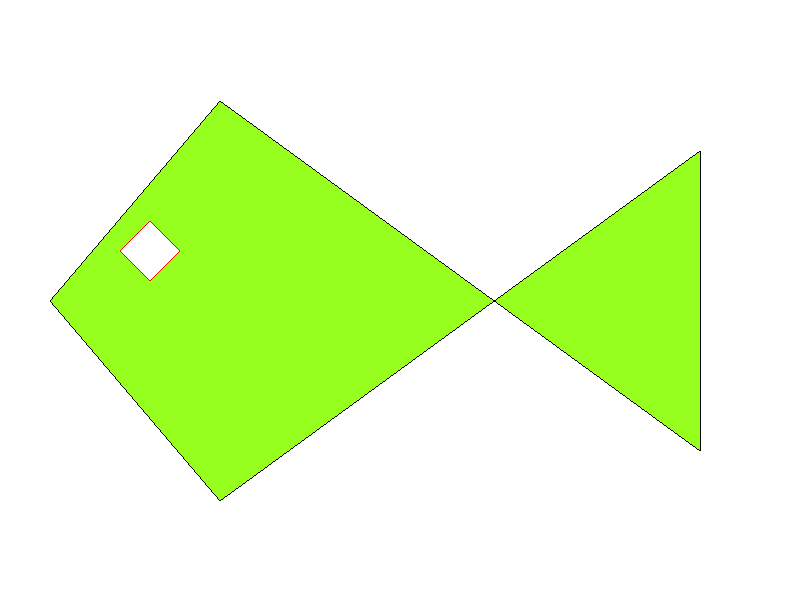
\includegraphics[width=\textwidth]{data/edit.png}}
  }
\end{column}
  \end{uloha}

  \begin{column}{0.65}
\begin{uloha}
  Uvažujme nasledovnú variáciu na tému Sierpińského koberca: máme parametre
  \prg!int x!, \prg!int d!,
  \prg!double i! a \prg!double f!. Chceme mať vzorku na obrázku rozmerov $x\times x$.
  Vzorka stupňa $d$  je štvorec so stranou dĺžky $ix$ umiestnený v strede obrázka.
  Navyše, ak $d>1$ tak v každom z rohov štvorca umiestnime vzorku stupňa $d-1$
  zmenšenú o faktor $f$ (a môže mať upravenú farbu). Napríklad pre
  hodnoty \vb{1000 6 0.45 0.5} by vzorka mohla vyzerať ako na obrázku vpravo.
  
  Napíš program, ktorý načíta zo vstupu parametre \vb{x d i f} a vypíše postupnosť príkazov,
  na základe ktorej program z predchádzajúcej úlohy vykreslí 
  vzorku.
\end{uloha}
\end{column}\hfill\begin{column}{0.3}
  {\setlength{\fboxsep}{0pt}
  \centerline{\fbox{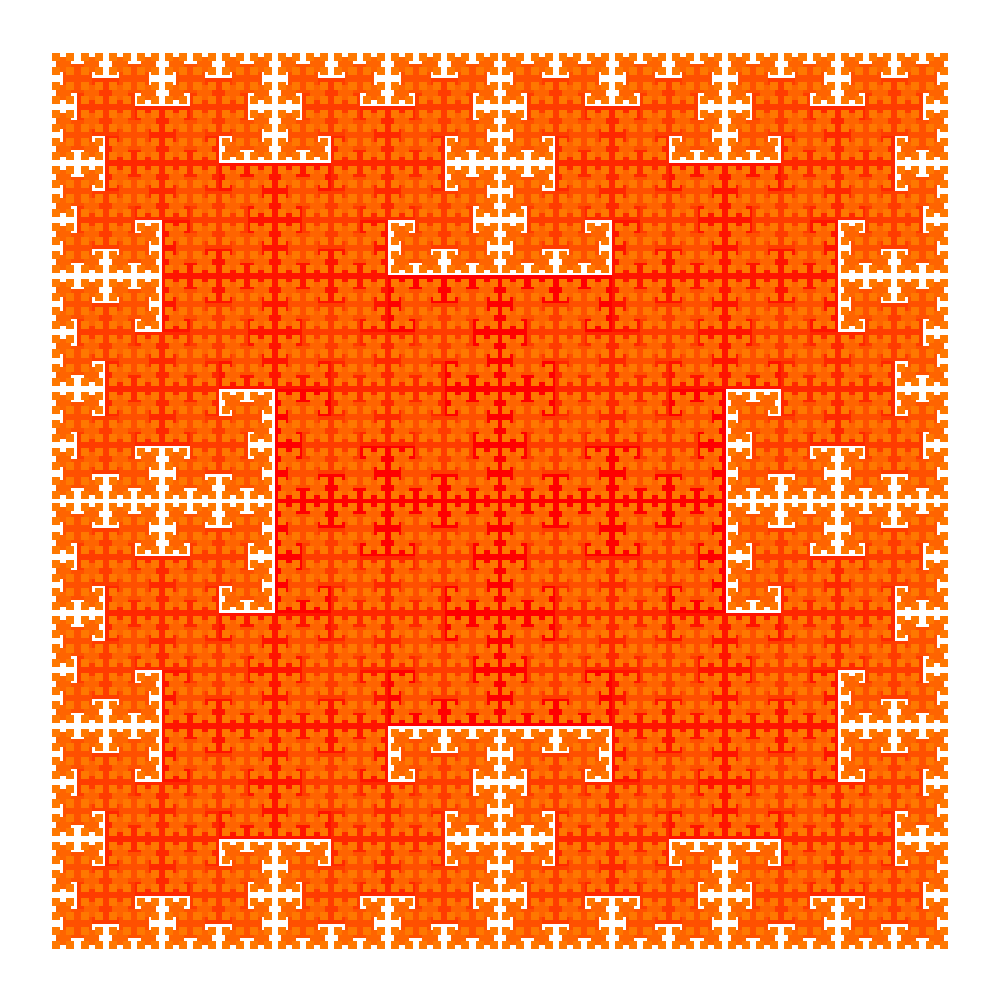
\includegraphics[width=\textwidth]{data/qq.png}}}
  }
\end{column}  


\indexItem{Mat}{sin, cos}
\section*{Odbočka: goniometrické funkcie $\sin$ a $\cos$}
\label{sect:sin_cos}

Niekedy je dobré vedieť kresliť čiaru nie do konkrétneho bodu, ale pod istým uhlom.
Povedzme, že máme uhol $\alpha$ okolo bodu $P$. Urobíme si hocikoľko
kolmíc takto:\\


\centerline{
  \begin{tikzpicture}[scale=0.6]
  \def\an{30}
  \def\len{8}
  \def\ra{0.2}
  \draw[blue](\len,0) -- (0,0) node[anchor=north east]{$P$} -- (\an:\len+1);
  \draw[blue](1,0) arc (0:\an:1) node[midway,anchor=west]{$\alpha$};

  \foreach \x[count=\i] in {3.5,4.8,7} {
    \draw(\x,-1) -- (\x,5);
    \node[anchor=north east] at (intersection of 0,0--10,0 and \x,-1--\x,5) {$A_{\i}$};
    \node[anchor=south east] at (intersection of 0,0--\an:100 and \x,-1--\x,5) {$B_{\i}$};
    \draw (\x,\ra) arc (90:180:\ra);
    \filldraw (\x-\ra/3,\ra/3) circle (.3pt);
  }
\end{tikzpicture}}


Všetky trojuholníky $\triangle A_1PB_1$,  $\triangle A_2PB_2$, \ldots sú podobné: majú
všetky uhly rovnako veľké. Preto sa zachovávajú aj pomery strán: napr.\footnote{%
  znakom $\nrm{\cdot}$ označujem dĺžku
}
$\nrm{A_3P} = 2\nrm{A_1P}$, preto aj $\nrm{B_3P}=2\nrm{B_1P}$. To znamená, že 
$\frac{\nrm{A_3P}}{\nrm{B_3P}}=\frac{2\nrm{A_1P}}{2\nrm{B_1P}}=\frac{\nrm{A_1P}}{\nrm{B_1P}}$.
Inými slovami, pomer $\frac{\nrm{A_iP}}{\nrm{B_iP}}$ je stále rovnaký, nezáleží, ktorú kolmicu
$A_iB_i$ si zoberieme. Tento pomer závisí iba od uhla $\alpha$, a označuje sa $\cos(\alpha)$
({\em kosínus}). Podobne pomer $\frac{\nrm{B_iA_i}}{\nrm{B_iP}}$ závisí iba od $\alpha$
a označuje sa $\sin(\alpha)$ ({\em sínus}).


Na čo je dobré poznať hodnoty $\sin(\cdot)$ a $\cos(\cdot)$? Povedzme, že chceš zistiť,
aké súradnice má bod $B$, ktorý je od $[0,0]$ vo vzdialenosti $r$ pod uhlom $\alpha$:


\centerline{
  \begin{tikzpicture}[scale=3.5]
  \def\an{40}
  \def\ra{0.4ex}
    \draw[thin,dotted,step=0.5](-0.5,-0.5) grid (1,1);
    \draw(1.1,0) -- (0,0) node[anchor=north east]{$O=[0,0]$} -- (\an:1.1);

    \draw[red](1ex,0) arc (0:\an:1ex) node[midway,anchor=west]{$\alpha$};
    \draw[thin,gray](-35:1) arc (-35:125:1);

    \draw[-{>[length=3ex,width=1ex]},thin,gray] (0,0) -- (110:1) node[midway,anchor=east]
    {$r$};

    \coordinate (B) at (\an:1);
    \draw[red](0,0)--(B) node[midway,anchor=south east]{$r$};
    \node[right=3mm of B]  {$B=[x,y]$};

    \draw[blue] (B) -- (B|-0,0) coordinate (A) node[midway, anchor=west] {$y = r\sin(\alpha)$};
    \node[anchor=north west] at (A) {$A$};
    
    \draw (A)+(0,\ra) arc (90:180:\ra);
    \filldraw (A)+(-\ra/3,\ra/3) circle (.1pt);

    \def\g{rgb:green,5;yellow,4;blue,2;black,3}
    \draw[thick,draw=\g](0,0)--(A) 
    node[midway,anchor=north]{\textcolor{\g}{$x = r\cos(\alpha)$}};
\end{tikzpicture}}


Keď si z $B$ spravíš kolmicu, dostaneš pravouhlý $\triangle AOB$, pričom $\nrm{OA}=x$,
$\nrm{AB}=y$ sú hľadané súradnice bodu $B$. Z predchádzajúceho vieš, že 
$\cos(\alpha)=\frac{\nrm{OA}}{\nrm{OB}}=\frac{x}{r}$, preto $x=r\cos(\alpha)$.
Rovnako dostaneš $y=r\sin(\alpha)$.


\indexItem{Prg}{\vb{cmath}}Funkcie \prg!sin! a \prg!cos! sú prístupné v knižnici, ktorá sa volá \vb{cmath}. 
Ich vstup ale nie je v stupňoch, ale v {\em radiánoch}. Ak obsah kruhu\footnote{%
  Urob si takýto pokus: zober si riešenie úlohy~\ref{uloha:kruh}
  a zrátaj v premennej \vb{S} počet čiernych pixelov. Na konci programu vypíš
  pomer čiernych pixelov k obsahu štvorca so stranou $r$, t.j. 
  \prg!(double)S / (double)(r * r)! Pre $r=10$ bol môj výsledok $3.05$, pre
  $r=500$ to už bolo $3.14128$ a pre $r=2450$ to bolo $3.14157$.

  
\begin{tikzpicture}
\begin{axis}[
  % title={\vb{pi}},  
  width=\textwidth, 
  height=4cm,
  xlabel={$r$},
  scaled x ticks=false,
  scaled y ticks=false,
  domain=0:800,
  xmin=0,
  xmax=800,
  ymin=3.05,
  ymax=3.15,
  /pgf/number format/.cd,
  1000 sep={}
  %legend cell align={left},
  %legend pos = south east
]
  \addplot+[no markers,magenta,thick,dotted] {3.1415926535};
  \addplot+[no markers,blue!40!cyan] table 
  [y expr=\thisrow{pi}, x expr=\thisrow{n} ]{data/pi.dat};
\end{axis}
\end{tikzpicture}

Výsledok sa blíži k číslu $3.1415926535\cdots$, čo je hodnota $\pi$.
}
s polomerom 1 
označíme $\pi$, tak jeho obvod je $2\pi$. Radiány merajú uhol dĺžkou príslušného
oblúka na jednotkovej kružnici: celý kruh, čiže $360^\circ$ je $2\pi$ radiánov,
pravý uhol je $\pi/4$ radiánov atď. Vo všeobecnosti $d$ stupňov je $d\frac{2\pi}{360}$
radiánov. V knižnici \vb{cmath} je definovaná konštanta \prg!M_PI!, ktorá
dosť presne reprezentuje číslo $\pi$. Nasledovný program:\\


\vbox{
\begin{lstlisting}[] 
#include <cmath>  
#include <iostream>

using namespace std;

int main() {
  cout << 3*cos(M_PI / 2.0) << " " << 3*sin(M_PI / 2.0) << endl;
}
\end{lstlisting}
}


má vypísať súradnice bodu, ktorý je vo vzdialenosti $3$ pod uhlom $\pi/2$ (t.j. kolmo
hore), teda by sa malo vypísať \vb{0 3}. V skutočnosti sa vypíše čosi ako 
\vb{1.83697e-16 3}. Zápis \vb{1.83697e-16} znamená $1.83697\cdot10^{-16}$, t.j. číslo
$0.000000000000000183697$. To je skoro nula, takže je to skoro správne. Nie je to presne nula,
lebo sa pri výpočte \vb{cos} prejavili problémy s presnosťou, ktoré si videl v 
predchádzajúcej časti.

\begin{uloha}
  Napíš program, ktorý na vstupe dostane číslo $n$ a vypíše postupnosť príkazov, na základe
  ktorých program z úlohy~\ref{uloha:editor} vykreslí vyplnený zelený pravidelný $n$-uholník.
\end{uloha}

\begin{uloha}
  Napíš program, ktorý na vstupe dostane číslo $n$ a $s$ a vyrobí príkazy pre program z 
  úlohy~\ref{uloha:editor}, ktorá nakreslia nasledovný útvar: zober si vrcholy pravidelného
  $n$-uholníka a spájaj ich čiarou s krokom $s$, t.j. spoj vrchol číslo $0$, 
  vrchol číslo $s$, vrchol číslo $2s$ a tak ďalej.
  Vnútro má byť vyfarbené žlto a vonkajšie cípy červeno. Napr. pre $n=7$, $s=3$ a pre
  $n=23$, $s=9$ sú tieto dva vzory:

  {
  \setlength{\fboxsep}{0pt}
  \begin{column}{0.45}
  \centerline{\fbox{
\includegraphics[width=0.9\textwidth]{data/m.7.3.png}}}
  \end{column}\hfill
  \begin{column}{0.45}
  \centerline{\fbox{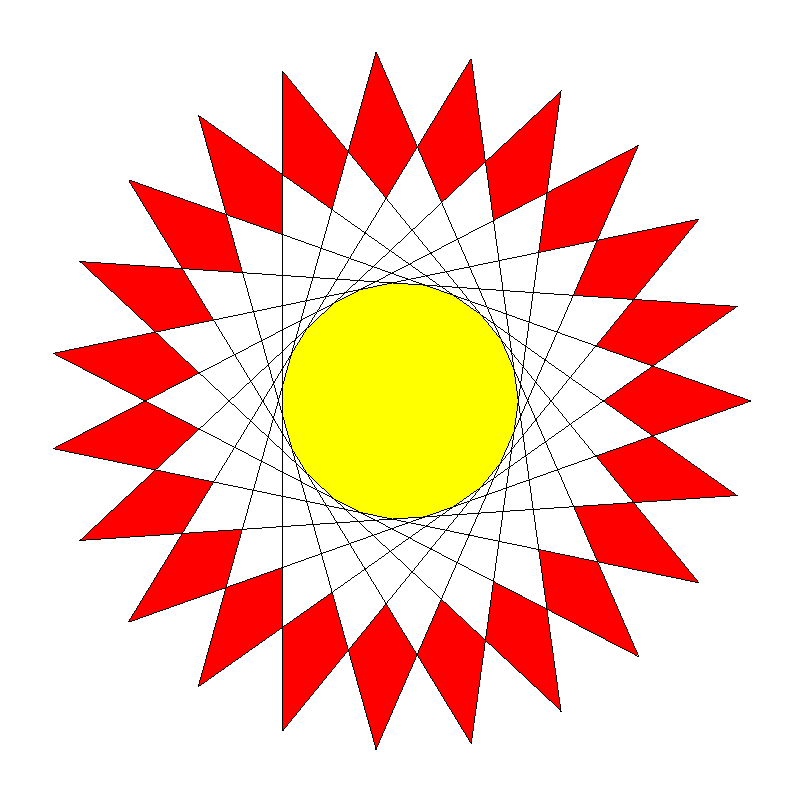
\includegraphics[width=0.9\textwidth]{data/m.23.9.png}}}
  \end{column}
  }
\end{uloha}

\def\ulohaTarget{None}
\vbox{
\begin{uloha}
  \indexItem{Alg}{korytnačia grafika}
  Korytnačia grafika pozostáva z postupnosti príkazov, každý na samostatnom riadku. 
  Príkazy sú takéto:
\def\tmp{\item \textcolor{magenta}}  
\begin{itemize}\itemsep=-1mm
    \tmp{\vb{i} {\em sirka vyska}} 
      (init) Toto je vždy prvý príkaz (a je v zozname iba
      raz). Nastaví rozmery obrázka. 
      \tmp{\vb{c} r g b} (color) Nastaví farbu na $\{r,g,b,255\}$.
    \tmp{\vb{u}} (pen up) Zdvihne pero -- nasledujúce posuny nekreslia.
    \tmp{\vb{d}} (pen down) Položí pero -- nasledujúce posuny kreslia.
    \tmp{\vb{f} x} (forward) Posunie sa dopredu o $x$.
    \tmp{\vb{l} a} (left) Otočí sa doľava o $a$ stupňov.
    \tmp{\vb{r} a} (right) Otočí sa doprava o $a$ stupňov.
    \tmp{\vb{s} meno} (save) Uloží obrázok a skončí.
\end{itemize}
Napíš program, ktorý načíta postupnosť príkazov korytnačej grafiky a vypíše
  postupnosť príkazov pre program z úlohy~\ref{uloha:editor}.
\end{uloha}
}
\def\ulohaTarget{File}


Na záver tejto časti skús rozšíriť korytnačiu grafiku o príkaz opakovania:

{\em
\def\tmp{\item \textcolor{magenta}}  
\begin{itemize}\itemsep=-1mm
      \tmp{\vb{R} cnt} (repeat) Blok príkazov po nasledujúci \vb{E} sa zopakuje
      {\em cnt} krát.
    \tmp{\vb{E}} (end) Koniec bloku opakovania.
\end{itemize}
}


Chceme, aby sa príkazy opakovania mohli vnárať, takže napr. program vľavo
urobí obrázok vpravo.

\begin{minipage}[t]{0.3\textwidth}\vspace{0pt}
\begin{Verbatim}
i 700 700
R 24
R 4
f 100
r 90
E
l 15
E
c 0 50 200
R 8
u
f 250
d
R 36
f 50
l 180
f 50
l 10
E
u
l 180
f 250
l 225
E
s logo.png
\end{Verbatim}
\end{minipage}
\hfill
\begin{minipage}[t]{0.7\textwidth}\vspace{0pt}{
  \setlength{\fboxsep}{0pt}
  \centerline{\fbox{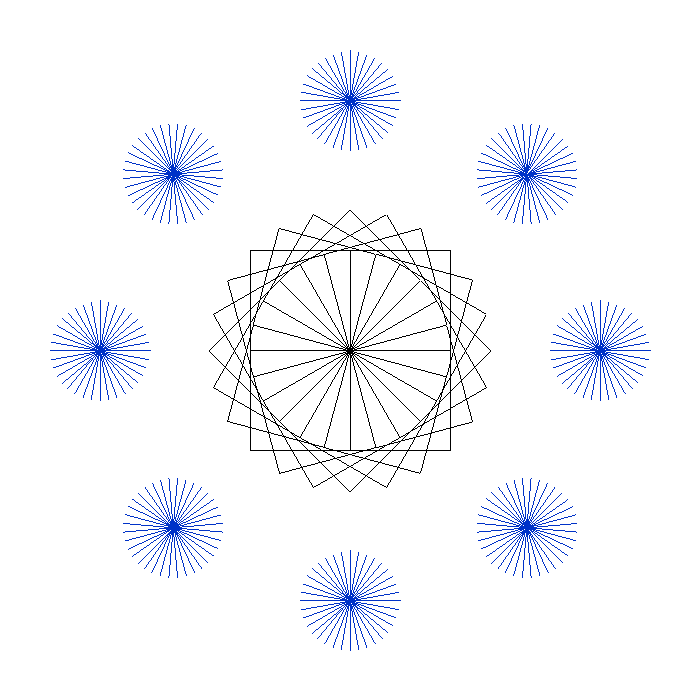
\includegraphics[width=\textwidth]{data/logo.png}}}
}
\end{minipage}


Na rozdiel od jednoduchšieho zadania bez cyklov, toto nemôžme riešiť tak, že 
príkazy čítame zo vstupu a priamo
vypisujeme príkazy pre kreslič, ale budeme si potrebovať všetky príkazy zapamätať.
Spravme si typ \vb{Prikaz}, v ktorom si budeme pamätať typ príkazu aj všetky
potrebné parametre (príkazy \vb{i} a \vb{s} ukladať nepotrebujeme, \vb{i} je vždy
na začiatku a \vb{s} je na konci: keď načítame zo vstupu \vb{s}, tak vygenerujeme
všetky zapamätané príkazy a skončíme). Okrem parametrov si v príkaze
\vb{R} budeme potrebovať pamätať terajší počet opakovaní pri vykonávaní 
a v príkaze \vb{E} si budeme potrebovať zapamätať pozíciu, kde je príslušný
príkaz \vb{R}. Celý typ by mohol vyzerať napr. takto:\\


\vbox{
\begin{lstlisting}[] 
struct Prikaz {
  char t;       // typ príkazu
  int r, g, b;  // pre príkaz 'c'
  double x;     // generický parameter pre príkazy 'l' 'r' 'f'
  int i, cnt;   // pre príkaz 'R'
  int addr;     // pre príkaz 'E'
};
\end{lstlisting}
}


Pri načítavaní vstupu si ukladáme príkazy do pamäte, pričom na príkazy \vb{R}
a \vb{E} použijeme zásobník ako v úlohe~\ref{uloha:zatvorky} na to, aby sme pre
každý príkaz \vb{E} našli zodpovedajúci príkaz \vb{R}. Začiatok programu z príkladu
by v poli vyzeral takto:


\centerline{
\begin{tikzpicture}[xscale=1.5,yscale=0.4]
    \def\cmd(#1)#2#3#4#5{
      \begin{scope}[shift={(#1,0)}]
        \draw (0,0) rectangle (1,5);
        \foreach \l [count = \i] in {addr,i,cnt,\ldots,t}{
          \node [anchor=south west] at (0,\i-1) {{\small\roboto \l}};
        }
        \foreach \v [count = \i] in {#5,#4,#3,{},'#2'}{
          \node [anchor=south west] at (0.5,\i-1) {{\small\roboto \textcolor{magenta}{\v}}};
        }
        \node [anchor=south] at (0.5,5) {$#1$};
      \end{scope}
      }

  \cmd(0)R{24}{0}{}
  \cmd(1)R{4}{0}{}
  \cmd(2)f{}{}{}
  \cmd(3)r{}{}{}
  \cmd(4)E{}{}{1}
  \cmd(5)l{}{}{}
  \cmd(6)E{}{}{0}
  \cmd(7)c{}{}{}
  \cmd(8)R{8}{0}{}
  \cmd(9)u{}{}{}
\end{tikzpicture}
}

Keď načítame celý program, začneme ho vyhodnocovať..
Budeme mať jednu globálnu premennú \vb{pc} (program counter),
v ktorej si budeme pamätať pozíciu práve vykonávaného príkazu. Bežné príkazy vždy 
spracujeme (tak, že vypíšeme na výstup príslušný príkaz pre kreslič) a zvýšime \vb{pc}.
V príkaze \vb{R} len zvýšime hodnotu \vb{i}. V príkaze \vb{E} sa pozrieme na hodnotu
\vb{i} v príslušnom \vb{addr}: ak sa rovná \vb{cnt}, vynulujeme ju a zvýšime \vb{pc},
ak nie, skočíme na príkaz \vb{R}. Ak sa pole príkazov volá \vb{prog} a
v premennej \vb{n} máme počet príkazov, vyhodnocovanie by vyzeralo zhruba takto:\\


\vbox{
\begin{lstlisting}[] 
void execute() {
  int pc = 0;
  while (pc < n) {
    if (prog[pc].t == 'R') {
      prog[pc].i++;
      pc++;
    } else if (prog[pc].t == 'E') {
      int jmp = prog[pc].addr;
      if (prog[jmp].i == prog[jmp].cnt) {
        prog[jmp].i = 0;
        pc++;
      } else {
        pc = jmp;
      }
    } else if .... 

    // tu sa spracujú ďalšie príkazy

  }
}


\end{lstlisting}
}


\begin{uloha}
  \label{uloha:logo}
  Naprogramuj korytnačiu grafiku s príkazmi cyklu.
\end{uloha}

\chapter{Adresy a smerníky (pointre)}

Technicky je celá pamäť počítača jedno veľké pole núl a jednotiek. V skutočnosti má
adresu iba každý ôsmy bit (celá pamäť teda vyzerá ako pole \prg!unsigned char!).
Keby na adrese 1 bola premenná \prg!int c;!, na adrese 5
premenná \prg!char a! a na adrese 6 premenná \prg!char b;!
začiatok pamäte by mohol vyzerať takto:


\centerline{\begin{tikzpicture}[scale=0.2]
  \def\var#1[#2]#3#4{%
    \pgfmathsetmacro{\tmp}{#1+8*#2}
    \draw[#4] decorate[
       decoration={brace, amplitude=2ex}]{
       (#1,1.8) -- (\tmp,1.8) node [align=center,midway,anchor=south,yshift=2ex] {\vb{#3}}
        };
   \draw[#4,thick] (#1,0) rectangle (\tmp,1.5);

  }
  \foreach \v [count=\i] in {
    0,1,0,0,0,1,1,1,
    0,1,1,0,0,0,0,1,
    0,1,1,0,1,1,1,0,
    0,1,1,0,0,1,0,0,
    0,1,1,0,0,0,0,1,
    0,1,1,0,1,1,0,0,
    0,1,1,0,0,1,1,0,
    0,0,0,0,0,0,0,0,
    0,1
  }{
    \draw (\i,0) rectangle node [anchor=center] {{\scriptsize\roboto \v}} (\i+1,1.5);
  }

  \foreach \i in {0,...,8}{
    \pgfmathsetmacro{\x}{\i*8+1.5}
  \draw[dotted] (\x,-0.1) -- (\x,-3) 
  node[draw, anchor = north west]{\scriptsize\vb{\i}};
}

  \var{9}[4]c{orange!60!black}
  \var{41}[1]a{cyan!60!black}
  \var{49}[1]b{green!60!black}
\end{tikzpicture}}


To, že nejaká premenná je na nejakej adrese, nie je v pamäti nijak špeciálne označené, je 
na programe, aby pristupoval na správne miesta v pamäti. V pamäti je vždy okrem tvojho 
programu veľa ďalších vecí, takže keď sa program spustí, operačný systém nájde v pamäti
voľné miesto a tvoj program bude používať adresy odtiaľ. Presná adresa premennej ti preto
sama osebe veľa nepovie, napriek tomu je užitočné ju vedieť. Až tak užitočné, že na to je
špeciálny operátor, \indexItem{Prg}{operátor \vb{\&}}\vb{\&}. Ak máš premennú \vb{x}, tak \vb{\&x} je jej adresa.
Skús si spustiť program:\\


\vbox{
\begin{lstlisting}[] 
#include <iostream>
using namespace std;

int c;
char a,b;

int main() {
  cout <<"adresa c: "<< (unsigned long)&c << endl;
  cout <<"adresa a: "<< (unsigned long)&a << endl;
  cout <<"adresa b: "<< (unsigned long)&b << endl;
} 
\end{lstlisting}
}

Vždy, keď ho spustíš, vypíšu sa iné čísla (tvoj program vždy dostane pridelenú
inú časť pamäte), ale môže to vyzerať napr. takto:

\begin{outputBox}
adresa c: 94082916049300
adresa a: 94082916049304
adresa b: 94082916049305
\end{outputBox}

V tomto prípade sa premenná \vb{c} uložila na adresu $94082916049300$ a zaberá 4 byty
(32 bitov). Za ňou, na adrese $94082916049304$ nasleduje premenná \vb{a}, ktorá zaberá
jeden byte, takže na nasledujúcej adrese $94082916049305$ je premenná \vb{b}.

\indexItem{Prg}{typ pointer}
Napriek tomu, že adresa je vždy číslo, operátor \prg!&! vracia v skutočnosti rôzne
typy. Pre každý typ \vb{T} (základný alebo vlastný
napr. \prg!int!, \prg!float!, \prg!Farba!,\ldots) existuje ďalší typ 
\cmd{adresa premennej typu \vb{T}} (hovorí sa aj {\em pointer na premennú typu \vb{T}}).
Tento nový typ sa označuje hviezdičkou za menom typu. Takže premenná typu \prg!int*! 
obsahuje adresu premennej, ktorá
je typu \prg!int!:\\



\vbox{
\begin{lstlisting}[] 
#include <iostream>
using namespace std;
int main() {
  int x = 258;       // premenná
  int *ax = &x;      // ok, ax je adresa x
  float *err = &x;   // <--  !! error: cannot convert 'int*' to 'float*'
  float* fx = (float*)(&x);  // ok, pretypovať sa dá
}
\end{lstlisting}
}

V poslednom riadku som použil pretypovanie; \vb{fx} je adresa miesta, kde by mala byť
premenná typu \prg!float!, aj keď v skutočnosti je tam uložená premenná typu \prg!int! 
(konkrétne \vb{x}). Ešte raz treba zdôrazniť: premenná \vb{ax} je krabička, v ktorej
je uložené číslo adresy\footnote{%
  V nasledujúcom obrázku ťa zámerne trochu klamem, v premennej typu \vb{int} sa väčšinou
  jej 4 byty ukladajú v opačnom poradí (tzv. {\em little endian}), ale pre
  naše účely to stačí takto.
}, na ktorej je uložená krabička s menom \vb{x}:

\centerline{\begin{tikzpicture}[scale=0.2]
  \def\var#1[#2]#3#4{%
    \pgfmathsetmacro{\tmp}{2+#1+8*#2}
    \draw[#4] decorate[
       decoration={brace, amplitude=2ex}]{
       (2+#1,1.8) -- (\tmp,1.8) node [align=center,midway,anchor=south,yshift=2ex] {\vb{#3}}
        };
   \draw[#4,thick] (2+#1,0) rectangle (\tmp,1.5);

  }
  \foreach \v [count=\i] in {
    1,0,
    0,0,0,0,0,0,0,0,
    0,0,0,0,0,0,0,0,
    0,0,0,0,0,0,0,1,
    0,0,0,0,0,0,1,0,
    %
    0,0,0,0,0,0,0,0,
    0,0,0,0,0,0,0,0,
    0,0,0,0,0,0,0,1,
    0,0,1,1,1,0,1,1,
    0,1
  }{
    \draw (\i,0) rectangle node [anchor=center] {{\scriptsize\roboto \v}} (\i+1,1.5);
  }

  \foreach \i in {0,...,8}{
    \pgfmathsetmacro{\x}{\i*8+3.5}
    \pgfmathtruncatemacro{\l}{\i+315}
  \draw[dotted] (\x,-0.1) -- (\x,-3) 
  node[draw, anchor = north west]{\scriptsize\vb{\l}};
}

  \var{1}[4]{x = 258}{orange!60!black}
  \var{33}[4]{ax = 315}{cyan!60!black}
\end{tikzpicture}}


\indexItem{Prg}{operátor \vb{*}} Opačný operátor k \prg!&! je \prg!*!: ak \prg!ax! je premenná typu \prg!int*!, tak
\prg!*ax! je premenná, ktorá je uložená na adrese, ktorá je uložená v  \vb{ax}
(hovoríme, že premenná \vb{ax} {\em ukazuje na premennú} \vb{*ax}). 
Teraz je vidno, prečo je
dobré mať zvlášť typ adresy pre každý typ: keď sa vyhodnocuje výraz \prg!*ax!, procesor
sa pozrie do premennej \vb{ax}, nájde tam číslo (napr. 315), pozrie sa na adresu $315$
a predpokladá, že tam bude premenná typu \prg!int!. Pozrie sa preto na nasledujúce
4 byty a vráti príslušné číslo. V predchádzajúcom príklade by \prg!cout << *ax << endl;! vypísalo $258$.
\prg!*ax! je naozaj premenná, takže sa dá do nej aj priraďovať. Príkazy
\prg!x = 47;! a \prg!(*ax) = 47;! urobia to isté. Takže program\\


\vbox{
\begin{lstlisting}[] 
#include <iostream>
using namespace std;
int main() {
  int x = 258;       
  int* ax = &x;  // ax ukazuje na x   
  (*ax) = 47;    // *ax je x
  cout << x << endl;
}
\end{lstlisting}
}
vypíše 47.


Treba rozlišovať medzi hviezdičkou pri vyrábaní premennej (napr. \prg!int *a!), ktorá znamená
\cmd{pointer na typ int} a hviezdičkou pred menom premennej (typu pointer) vo výraze,
ktorá znamená \cmd{hodnota na adrese}. Skús prečítať nasledovný program:\\


\vbox{
\begin{lstlisting}[] 
#include <iostream>
using namespace std;

int main() {
  int a = 7, x = 6;  // a,x sú premenné typu int
  int *b = &a;       // b ukazuje na a
  int **c = &b;      // c ukazuje na b
  int *d = *c;       // *c je premenná b, preto tento príkaz
                     // je rovnaký ako int* d = b;
  **c = 18;
  b = &x;            // teraz b ukazuje na x
  **c = 42;          
  cout << a << " " << x << endl;
}
\end{lstlisting}
}

Po prvých štyroch riadkoch by to v pamäti mohlo vyzerať ako na obrázku vľavo.
V príkaze \prg!**c=18;! je \prg!*c! premenná \prg!b! a \prg!*b! je premenná \prg!a!,
preto sa do premennej \prg!a! zapíše 18.
Nasledujúci príkaz \prg!b=&x! spôsobí, že v \vb{b} bude uložená adresa \vb{x} ako na 
obrázku vpravo. Preto v príkaze \prg!**c=42! je \prg!*c! premenná \prg!b!
a \prg!*b! je premenná \prg!x!, takže program vypíše \vb{18 42}.


\def\var(#1)#2#3#4{%
  \draw (0,0.5-#1)  node[anchor=east]{\vb{#3}};
  \draw (0.2,-#1) rectangle node[align=center]{\vb{#2}} (1.2,1-#1);
  \draw (1.4,0.5-#1) node[anchor=west]{\textcolor{magenta}{\vb{#4}}};
}

\def\ptr(#1,#2)[#3] {
  \draw[blue,-{>[length=4pt,width=2.5pt]}] (1.7,0.5-#1) to[out=#3,in=-#3] (1.7,0.5-#2);
}

\begin{column}{0.45}
\begin{tikzpicture}[yscale=0.4,xscale=1.4]
  \node[anchor=east] at (0,0.8){{\em adresa}};
  \foreach \val/\addr/\name[count=\i] in {7/42380/a,6/42384/x,42380/42388/b,
     42388/42396/c,42380/42404/d}  {
    \var(\i){\val}{\addr}{\name}
  }
  \draw(0,0.5-6) node[anchor=east]{\vb{42412}};
  \draw[draw=none] (0.2,-6) rectangle node[align=center]{\vb{\ldots}} (1.2,1-6);
  \ptr(3,1)[75]
  \ptr(4,3)[60]
  \ptr(5,1)[65]
\end{tikzpicture}
\end{column}
\hfill
\begin{column}{0.45}
\begin{tikzpicture}[yscale=0.4,xscale=1.4]
  \node[anchor=east] at (0,0.8){{\em adresa}};
  \foreach \val/\addr/\name[count=\i] in {18/42380/a,6/42384/x,42384/42388/b,
     42388/42396/c,42380/42404/d}  {
    \var(\i){\val}{\addr}{\name}
  }
  \draw(0,0.5-6) node[anchor=east]{\vb{42412}};
  \draw[draw=none] (0.2,-6) rectangle node[align=center]{\vb{\ldots}} (1.2,1-6);
  \ptr(3,2)[60]
  \ptr(4,3)[60]
  \ptr(5,1)[65]
\end{tikzpicture}
\end{column}


S pomocou pointrov môžeš mať funkciu, ktorá ako keby menila svoje parametre.
Porovnaj tieto dva programy:


\begin{column}{0.45}
\vbox{
\begin{lstlisting}[] 
#include <iostream>
using namespace std;

void pridaj(int a) { 
  a = a + 1; 
}

int main() {
  int x = 7;
  pridaj(x);
  cout << x << endl;
} 
\end{lstlisting}
}
\end{column}
\hfill
\begin{column}{0.45}
\vbox{
\begin{lstlisting}[] 
#include <iostream>
using namespace std;

void pridaj(int *a) {
  (*a) = (*a) + 1;
}

int main() {
  int x = 7;
  pridaj(&x);
  cout << x << endl;
}
\end{lstlisting}
}
\end{column}

V ľavom programe sa vyrobí svet funkcie \vb{main} a v ňom premenná \vb{x}. Pri
volaní funkcie \vb{pridaj} sa vyrobí nový svet s premennou \vb{a} a nastaví sa jej
hodnota na $7$. Potom sa vykoná funkcia \vb{pridaj}, takže v premennej \vb{a}
bude $8$. Svet funkcie \vb{pridaj} potom zanikne a v \vb{main} sa vypíše hodnota 
\vb{x}, t.j. 7. V pravom programe sa vyrobí svet funckie \vb{pridaj}, ale 
premenná \vb{a} sa nastaví na adresu premennej \vb{x} (premenná \vb{x} je vo svete 
funkcie \vb{main}, ale svety a premenné sú vec programu a kompilátora; pri prístupe
do pamäte vo výslednej binárke nehrajú rolu).
Preto vo svete \vb{pridaj}  výraz \vb{*a} označuje premennú \vb{x} zo sveta funkcie \vb{main}
a funkcia \vb{pridaj} zvýši hodnotu \vb{x} o 1. Keď svet \vb{pridaj}
zanikne, zanikne premenná \vb{a}, ale hodnota \vb{x} ostane zmenená.


\def\var(#1)#2#3#4{%
  \draw (0,0.5-#1)  node[anchor=east]{\vb{#3}};
  \draw (0.2,-#1) rectangle node[align=center]{\vb{#2}} (1.2,1-#1);
  \draw (1.4,0.5-#1) node[anchor=west]{\textcolor{magenta}{\vb{#4}}};
}

\def\ptr(#1,#2)[#3] {
  \draw[blue,-{>[length=4pt,width=2.5pt]}] (1.7,0.5-#1) to[out=#3,in=-#3] (1.7,0.5-#2);
}

\def\kon(#1)#2{ \draw(0,0.5-#1) node[anchor=east]{\vb{#2}};
  \draw[draw=none] (0.2,-#1) rectangle node[align=center]{\vb{\ldots}} (1.2,1-#1);
}

\def\world(#1)#2#3{
  \draw[thick,#3](-1,-#1) -- (2,-#1) node[anchor=west]{\vb{#2}};
}
\begin{column}{0.45}
\begin{tikzpicture}[yscale=0.4,xscale=1.4]
  \node[anchor=east] at (0,0.8){{\em adresa}};
  \world(0){main}{orange}
  \world(1){pridaj}{blue!70!gray}

  \foreach \val/\addr/\name[count=\i] in {7/873200/x,8/873204/a}  {
    \var(\i){\val}{\addr}{\name}
  }
  
  \kon(3){873208}
\end{tikzpicture}
\end{column}
\hfill
\begin{column}{0.45}
\begin{tikzpicture}[yscale=0.4,xscale=1.4]
  \node[anchor=east] at (0,0.8){{\em adresa}};
  \world(0){main}{orange}
  \world(1){pridaj}{blue!70!gray}

  \foreach \val/\addr/\name[count=\i] in {8/873200/x,837200/873204/a}  {
    \var(\i){\val}{\addr}{\name}
  }
  \ptr(2,1)[70]
  \kon(3){873208}
\end{tikzpicture}
\end{column}

\indexItem{Prg}{pointrová aritmetika}
S pointrami sa dajú robiť aj aritmetické operácie, ale trochu inak ako s normálnymi
číslami. Ak k premennej typu pointer pripočítaš 1, zväčší sa o veľkosť typu, na ktorý
ukazuje (v prípade \prg!int! je to 4). Veľkosť typu sa dá zistiť pomocou príkazu
\prg!sizeof!. V poli sú prvky uložené za sebou, takže napr. program

\vbox{
\begin{lstlisting}[] 
#include <iostream>
using namespace std;

int main() {
  int a = {12, 35};  // a[0] a a[1] nasledujú v pamäti za sebou
  int *x = &(a[0]);
  cout << *x << " " << *(x + 1) << endl;
  cout << (unsigned long)x << " + " << sizeof(int) << " = "
       << (unsigned long)(x + 1) << endl;
}
\end{lstlisting}
}

mi vypísal

\begin{outputBox}
12 35
140727139715200 + 4 = 140727139715204
\end{outputBox}

Pri práci s pointrami si treba dávať pozor na to, aby vždy ukazovali do pamäte,
ktorá patrí tvojmu programu. Môžeš napríklad napísať \prg!int *a = (int*)856;!
a nič zlé sa nestane. Ale ak by si potom chcel urobiť \prg!*a = 3;!, program skončí
s hláškou \vb{Segmentation fault}: pamäť na adrese 856 ti nepatrí. Je dobrý zvyk
do pointrov, ktoré zatiaľ neukazujú na nič rozumné, priradiť 0 (adresa 0 ti celkom
isto nepatrí) a pred použitím urobiť test. Môžeš napísať \prg!int *a = 0;!, alebo
\prg!int *a = NULL;! alebo \prg!int *a = nullptr;!, všetky tri spravia v konečnom 
dôsledku to isté.


\indexItem{Prg}{pointer na pole a pole pointrov}
Samozrejme, pointer môže ukazovať aj na vlastné typy a dokonca aj na polia.
To môže byť trochu zamotané. Napr.\\

\vbox{
\begin{lstlisting}[] 
int a, b, c;
int *p[3] = {&a, &b, &c};

*(p[0]) = 5;
*(p[1]) = 25;
*(p[2]) = 225;

cout << a << " " << b << " " << c << endl;
\end{lstlisting}
}

vyrobí trojprvkové pole \vb{p}, ktorého prvky budú pointre na premenné typu \prg!int!
a naplní ho pointrami na premenné \vb{a, b, c}. Preto potom \prg!p[0]! je pointer
na premennú \prg!a! a teda \prg!*(p[0]) = 5;! priradí 5 do premennej \vb{a}
a program vypíše \vb{5 25 225}. Zápis \prg!int *p[3]! čítaš najprv od 
názvu premennej doprava
a potom doľava zvyšok: \cmd{pole dĺžky 3, ktorého prvky sú pointre na int}.
Ak napíšeš \prg!int (*p)[3]!, znemená to \cmd{pointer na pole dĺžky 3,
ktorého prvky sú int}:\\

\vbox{
\begin{lstlisting}[] 
int a[3] = {1, 2, 3};
int(*p)[3] = &a;

cout << (*p)[1] << endl;
\end{lstlisting}
}

Ako by si zapísal pole dĺžky 2, ktorého prvky sú polia dĺžky 3? \prg!int a[2][3]!
Pripomína ti to niečo? Presne tak, je to dvojrozmerné pole. Dvojrozmerné pole
je vlastne pole riadkov, ktorého prvky sú polia stĺpcov. Preto môžeš mať\\

\vbox{
\begin{lstlisting}[] 
int a[2][3] = {{1, 2, 3}, {4, 5, 6}};
int(*p)[3] = &(a[0]);

cout << (*(p+1))[1] << endl;
\end{lstlisting}
}

V tomto prípade \vb{a} je pole dĺžky 2, ktorého prvky sú trojprvkové polia,
preto \vb{a[0]} je trojprvkové pole.
\vb{p} je pointer na trojprvkové pole, preto môžeš napísať \prg!p=&(a[0])!.
Potom \prg!p+1! ukazuje do pamäte o 12 bytov ďalej (\prg!sizeof(int[3])! je 12).
Prvky v poli sú uložené za sebou, preto 
ak \prg!p! ukazuje na \prg!a[0]!, tak \prg!p+1! ukazuje na \prg!a[1]!.
Napokon \prg!*(p+1)! je to isté, čo \prg!a[1]!, preto \prg!(*(p+1))[1]! vypíše 5.


\chapter{Polia revealed}

Hovoril som ti, že pole nie je premenná, ale veľa premenných, a preto sa
správa zvláštne (napr. si nesmel posielať pole ako parameter do funkcie,
nesmel si priraďovať a pod.). V skutočnosti je pole konštantný\footnote{%
S označením \prg!const! sme sa už stretli v tvare \prg!const int n = 100;!: 
ak ho napíšeš pred definíciu premennej,
znamená to, že premenná sa už potom nesmie meniť. 
Podobne môže byť \prg!const int *a = &x;!
}pointer.
Keď napíšeš \prg!int a[10];! vyrobí sa v pamäti 10 premenných typu \prg!int!
a \vb{a} je \prg!const! pointer na prvú z nich. Označenie indexu \vb{[ ]}
je v skutočnosti iba skratka za výraz s hviezdičkou: \prg!a[i]! znamená
\prg!*(a+i)! pre hocijaký pointer \vb{a}. Rôzne spôsoby prístupu k
prvkom poľa sú v nasledujúcom programe:

\vbox{
\begin{lstlisting}[] 
#include <iostream>
using namespace std;

int main() {
  int a[10];
  int *b, *c;
  int i;
  a = b; // <-- !! chyba, a je const
  c = a + 1;  // c ukazuje na a[1]

  b = a;  // b ukazuje na a[0]
  for (i = 0; i < 10; i++) {
    *b = i + 1;  // *b zapisuje do poľa a
    b = b + 1;   // presuň b na ďalší prvok poľa
  }

  cout << a[0] << endl;
  for (i = 0; i < 9; i++)
    cout << c[i] << endl;  // c ukazuje na a[1], preto
                           // c[i] je a[i+1]

  *(a + 5) = 14;                // *(a+5) je a[5]
  for (b = a; b < a + 10; b++)  // k b sa dá pripočítavať číslo aj takto
    cout << *b << " ";
  cout << endl;
}
\end{lstlisting}
}


Teraz by malo byť jasné, ako sa dá posielať pole ako parameter do funkcie: stačí,
aby bol typu pointer. Treba si ale vždy poslať aj veľkosť poľa ako samostatný parameter:

\begin{lstlisting}[] 
void napln_pole(int n, int *a) {
  int i;
  for (i = 0; i < n; i++)
    a[i] = i * i;
}

int main() {
  int a[10];
  napln_pole(10, a);
  int i;
  for (i = 0; i < 10; i++)
    cout << a[i] << " ";
  cout << endl;
}
\end{lstlisting}

Tento program vypíše \vb{0 1 4 9 16 25 36 49 64 81}. Len pripomeniem: ak by si v tomto
programe zmenil riadok \prg!int a[10];! na \prg!int a[3];!, program by fungoval rovnako,
akurát, že vo funkcii \vb{napln\_pole} by sa zapisovalo aj do pamäte, ktorá nebola
rezervovaná poľom \vb{a}. Ak sú tam nejaké premenné tvojho programu (napr. \vb{i}), 
prepíšu sa. Ak tá
pamäť tvojmu programu nepatrí, príde náš priateľ \vb{segfault}.



Dvojrozmerné pole je pole, ktorého prvkami sú polia. Preto ak máš \prg!int a[2][3]!,
tak \vb{a} je (konštantný) pointer na trojprvkové pole typu \prg!int!. Preto 
\prg!*(a+1)! je to isté, čo \prg!a[1]!, čiže trojprvkové pole typu \prg!int!
(t.j. môžeš napísať \prg!int *q = *(a+1);! a potom \prg!q! bude ukazovať na
prvý prvok poľa \prg!a[1]!, čiže na druhý riadok poľa \prg!a!).
Z toho celého vyplýva, že dvojrozmerné pole je v pamäti vlastne jednorozmerné
pole uložené rovnako, ako sme to mali v kapitole~\ref{sect:2dpolia}.
Na to, aby si k nemu tak mohol pristupovať, treba ho pretypovať, takže môžeš
napísať \prg!int *p = (int *)a;!. To je zároveň aj najjednoduchší spôsob, ako
posielať dvojrozmerné pole ako parameter do funkcie.\\

\vbox{
\begin{lstlisting}[] 
int main() {
  int a[2][3];
  int i, j, k = 1;

  for (i = 0; i < 2; i++)      // naplníme pole po riadkoch 
    for (j = 0; j < 3; j++) {
      a[i][j] = k;
      k++;
    }

  int *q = *(a + 1);           // q ukazuje na druhý riadok
  for (int i = 0; i < 3; i++) 
    cout << q[i] << endl;

  int *p = (int *)a;          // pohľad na a ako na 1D pole 
  for (i = 0; i < 6; i++) 
    cout << p[i] << " ";
  cout << endl;
} 
\end{lstlisting}
}


 Malá odbočka: mechanizmus posielania parametrov pointrami sa používa aj v iných 
programovacích jazykoch, ale častokrát ``pod kapotou''. Napríklad Python posiela
základné typy ako parametre (tzv. {\em volanie hodnotou}), ale na zoznamy a iné zložité
typy posiela pointer (tzv. {\em volanie referenciou}). Pythonovský program\\

\vbox{
\begin{lstlisting}[language=python] 
def zelena(x):
    x = 42

def modra(x):
    x[0] = 42

a = 1
zelena(a)
print(a)

b = [1, 2, 3]
modra(b)
print(b)
\end{lstlisting}
}

vypíše

\begin{outputBox}
1
[42, 2, 3]
\end{outputBox}

Do funkcie \vb{zelena} sa poslalo číslo, preto sa menila hodnota lokálnej premennej
vo svete funkcie \vb{zelena} (ktorá spolu s jej svetom zanikla), do funkcie \vb{modra}
sa poslal pointer na zoznam \vb{b}. Tento spôsob volania dáva zmysel, lebo väčšinou je to
presne to, čo chceš, ale pre začínajúcich programátorov to niekedy môže byť mätúce.
Koniec malej odbočky.

 Vyriešili sme, ako posielať polia ako parametre, ale stále nám ostáva problém 
s globálnymi poľami. Pamätáš sa, že keď sme pri kreslení obrázkov chceli mať globálne
pole, museli sme ho vyrobiť tak, aby už v čase kompilácie bola známa jeho veľkosť. 
Riešili sme to tak, že sme pole spravili dostatočne veľké a používali z neho iba 
tak veľký kus, ako sme potrebovali. Toto evidentne nie je najlepší prístup.\indexItem{Prg}{dynamická alokácia: \vb{new[]} a \vb{delete[]}} 
Lepšie riešenie je tzv. {\em dynamická alokácia}: príkaz \prg!new int[100];! 
vyhradí v odľahlom kúte pamäte miesto na 100 premenných typu \prg!int! a vráti pointer
naň. Toto miesto je vyhradené pre tvoj program, ale vrátený pointer je jediný spôsob,
ako sa k tej pamäti dostať: ak si ho neuložíš do premennej (alebo ju neskôr zabudneš),
pamäť stále ostane vyhradená pre tvoj program, ale ten sa k nej už nikdy nebude môcť dostať.
Ak už alokovanú pamäť nepotrebuješ, treba ju vrátiť systému príkazom \prg!delete[]!. Treba
byť opatrný, lebo to, či je pamäť vyhradená, alebo nie, nijak nevidno. Dobrý zvyk 
je hneď po volaní \prg!delete[]! priradiť do odalokovanej premennej \prg!nullptr!.\\

\vbox{
\begin{lstlisting}[] 
#include <iostream>
using namespace std;

int *a = (int *)12345;

void rob_nieco() {
  int i;
  for (i = 0; i < 100; i++) a[i] = 42;
}   

void vypis(int x) { cout << x << ": " << (unsigned long)a << endl; }
  
int main() {
  vypis(1);
  a = new int[100];
  vypis(2);     // a ukazuje na pridelenú pamäť
  rob_nieco();  // v poriadku, píšem do svojej pamäte
  delete[] a;   // pridelená pamäť sa označila ako voľná
  vypis(3);     // hodnota a sa nezmenila, stále ukazuje na to isté miesto,
                // ale tá pamäť mi už nepatrí
  rob_nieco();  // <-- !! toto by bol problém - systém medzitým mohol 
                // tú pamäť dať niekomu inému
}
\end{lstlisting}
}

Tento program vypíše napr.

\begin{outputBox}
1: 12345
2: 94751025169088
3: 94751025169088
\end{outputBox}

 Pri priraďovaní si treba dávať pozor, 
hlavne ak je pointer na dynamicky alokovanú pamäť súčasť zloženého typu, napr.

\vskip 2ex
\vbox{
\begin{lstlisting}[] 
struct Kvak {
  int *a, b, c[2];
};
\end{lstlisting}
}

Ak napíšeš

\begin{lstlisting}[] 
Kvak x, y;
x.a = new int[100];
y.a = new int[100];
\end{lstlisting}

a ešte ponastavuješ ďalšie hodnoty, môže to v pamäti vyzerať takto:


\def\var(#1)#2#3{%
  \draw (0.2,-#1) rectangle node[align=center](v#1) {\vb{#3}} (1.2,1-#1);
  \draw (0,0.5-#1) node[anchor=east]{\textcolor{magenta}{\vb{#2}}};
}

\def\ptr(#1,#2)[#3] {
  \draw[blue,-{>[length=4pt,width=2.5pt]}] (1.7,0.5-#1) to[out=#3,in=-#3] (1.7,0.5-#2);
}

\def\world(#1)#2#3{
  \draw[thick,#3](-1,-#1) -- (2,-#1) node[anchor=west]{\vb{#2}};
}

\def\kon(#1){ 
  \draw[draw=none] (0.2,-#1) rectangle node[align=center]{\vb{\ldots}} (1.2,1-#1);
}
  
\def\godot#1{\filldraw[blue,scale=0.6](#1) circle (0.4ex and 1.4ex);}

\begin{tikzpicture}[yscale=0.4,xscale=1.4]

  \var(0){x.a}{}
  \var(1){x.b}{1}
  \var(2){x.c[0]}{2}
  \var(3){x.c[1]}{3}
  \var(4){y.a}{}
  \var(5){y.b}{4}
  \var(6){y.c[0]}{5}
  \var(7){y.c[1]}{6}
  \world(-1){x}{orange}
  \world(3){y}{olive}
  \kon(8)

  \coordinate (a1) at (3,-0.5);
  \coordinate (a2) at (3,-4.5);

  \foreach \f/\t/\l in {v0/a1/{},v4/a2/{inde\ }}{
  \godot{\f}
  \draw[blue,-{>[length=8pt,width=5pt]}] (\f) to [out=0,in=180] (\t);
  \draw (\t)++(0,-0.5) rectangle node[align=center]{400 bytov niekde \l v pamäti} ++(5,1);
  }
\end{tikzpicture}

keď potom napíšeš \prg!y=x!, stane sa toto:

\begin{tikzpicture}[yscale=0.4,xscale=1.4]

  \var(0){x.a}{}
  \var(1){x.b}{1}
  \var(2){x.c[0]}{2}
  \var(3){x.c[1]}{3}
  \var(4){y.a}{}
  \var(5){y.b}{1}
  \var(6){y.c[0]}{2}
  \var(7){y.c[1]}{3}
  \world(-1){x}{orange}
  \world(3){y}{olive}
  \kon(8)

  \coordinate (a1) at (3,-0.5);
  \coordinate (a2) at (3,-4.5);

  \foreach \f/\t/\l in {v0/a1/{},v4/a2/{inde\ }}{
  \godot{\f}
  \draw (\t)++(0,-0.5) rectangle node[align=center]{400 bytov niekde \l v pamäti} ++(5,1);
  }

  \draw[blue,-{>[length=8pt,width=5pt]}] (v0) to [out=0,in=180] (3,-0.35);
  \draw[blue,-{>[length=8pt,width=5pt]}] (v4) to [out=0,in=180] (3,-0.65);
\end{tikzpicture}

Navždy si stratil 400 bytov pamäte a navyše ak napíšeš \prg!delete[] x.a; delete[] y.a;!
program zhavaruje s chybou

\begin{outputBox}
free(): double free detected in tcache 2
Aborted
\end{outputBox}

lebo si dvakrát odalokovával tú istú pamäť (aj keď si sa k nej dostal z iných pointrov).

\begin{uloha}
  Npaíš funkciu, kotrá ako parametre dostane číslo $n$ a pointer na  pole $n$
  čísel a toto pole v pamäti otočí. Napr. ak pred volaním bolo $n=5$
  a v poli boli čísla \vb{1 2 3 4 5} po volaní tam bude \vb{5 4 3 2 1}.
\end{uloha}

\begin{uloha}
  \label{uloha:arraycopy}
  Napíš funkciu, ktorá ako parametre dostane číslo $n$ a pointer na pole $n$
  čísel a toto pole skopíruje (t.j. vráti pointer na iné pole, v ktorom budú
  tie isté prvky).
\end{uloha}

\begin{uloha}
  Napíš funkciu, ktorá ako parametre dostane číslo $n$, pointer na  pole $n$
  čísel a číslo $k$ a pole v pamäti cyklicky posunie o $k$ miest.
  Napr. ak $n=5$, $k=2$ a pole bolo \vb{1 2 3 4 5}, tak po volaní funkcie
  pole bude \vb{3 4 5 1 2}.
\end{uloha}

\begin{uloha}
  \label{uloha:primetest}
  Napíš funkciu, ktorá dostane parameter $n$ a vráti pointer na dynamicky alokované
  pole, v ktorom bude prvých $n$ prvočísel\footnote{%
    \indexItem{Mat}{prvočíslo}
    Prvočíslo je číslo $p$, ktoré nemá iných deliteľov ako 1 a $p$. Inými slovami
    \prg~p\%i != 0~ pre všetky $i<p$. Ak to chceš jemne vylepšiť, premysli si,
    že ak má číslo $a$ nejakého deliteľa, tak má aj deliteľa veľkosti 
    nanajvýš $\sqrt{a}$. Ak na začiatku napíšeš \prg!#include<cmath>!, môžeš
    použiť funkciu \prg!sqrt(x)! na výpočet $\sqrt{x}$ (vracia typ double).
    }.
\end{uloha}

\begin{uloha}
  \label{uloha:merge}
  Napíš funkciu, ktorá dostane ako parametre dve utriedené polia veľkostí $n$ a $m$
  (t.j. dostane $n$, $m$ a dva pointre) a vyrobí utriedené pole dĺžky $n+m$, 
  ktoré obsahuje prvky z oboch vstupných polí.
\end{uloha}

\begin{uloha}
  \label{uloha:mergesort}\indexItem{Alg}{MergeSort}
  Napíš funkciu, ktorá dostane ako parameter $n$ a dynamicky alokované pole
  dľžky $n$ a utriedi ho pomocou algoritmu {\em Merge Sort}. Algoritmus {\em Merge
  Sort} je rekurzívny algoritmus, ktorý funguje takto: pole dĺžky $1$ je utriedené,
  netreba nič robiť. Ak má pole dĺžku aspoň 2, rozdeľ ho na dve polovice (t.j.
  vyrob si nové polia správnej dĺžky, prekopíruj do nich prvky z pôvodného poľa)
  a rekurzívne obe utrieď. Potom použi algoritmus z úlohy~\ref{uloha:merge} na to,
  aby si vyrobil výsledné pole (nezabudni vrátiť pamäť z pomocných polí).
\end{uloha}

\begin{uloha}
  \label{uloha:sortbody}
  Majme typ \prg!struct Bod{float x,y;};! Napíš funkciu, ktorá ako parameter
  dostane pole bodov a utriedi ho\footnote{napr. pomocou algoritmu {\em Insertion Sort}
  z kapitoly~\ref{sect:zlozitost}} podľa $x$-ovej súradnice.
\end{uloha}

\begin{uloha}
  Na vstupe je číslo $n$, a pole $n$ čísel \vb{t[0]},\ldots,\vb{t[n-1]}, ktoré 
  predstavujú časované bomby: \vb{i}-ta bomba vybuchne po \vb{t[i]} sekundách.
  Pyrotechnik vie každú sekundu zneškodniť jednu bombu. Napíš program, ktorý
  zistí, či sa mu podarí zneškodniť všetky bomby. Napr. pre vstup \vb{9 3 2 5 2} 
  sa mu to podarí: v prvej sekunde zneškodní poslednú bombu, preto v druhej sekunde
  budú časovače na bombách ukazovať \vb{8 2 1 4 $\times$}. Pyrotechnik akurát včas zneškodní
  bombu číslo $2$, takže bude stav \vb{7 1 $\times$ 3 $\times$}, opäť v poslednej
  sekunde zneškodní bombu č.1: \vb{6 $\times$ $\times$ 2 $\times$} a posledné dve bomby
  zneškodní s prehľadom. Pre vstup \vb{3 4 3 7 1 3} sa mu to ale nepodarí.
\end{uloha}

\chapter{Zásobník ako vlastný typ}
\label{sect:zasobnik}

V kapitole~\ref{sect:stack} sme používali zásobník tak, že sme mali pole fixnej
veľkosti a jednu premennú, ktorá udávala aktuálny počet prvkov v zásobníku. Keby sme chceli
mať viac zásobníkov, mali by sme viac polí a viac premenných. Aby sme v tom udržali
poriadok, je dobré spraviť si vlastný typ, kde budú obe veci pokope, napr.

\vskip 2ex
\vbox{
\begin{lstlisting}[] 
#include <iostream>
using namespace std;

const int N = 100000;

struct Stack {
  int a[N], n;
};
  
int main() {
  Stack s1, s2;

  s1.n = 0;
  s2.n = 0;

  // pridaj prvok
  s1.a[n]=1;
  s1.n++;
}
\end{lstlisting}
}


Takáto definícia má dva problémy: vždy, keď vyrobíme zásobník, vyhradí sa v pamäti
veľké pole, aj keby sme dopredu vedeli, že budeme potrebovať menej. Druhý problém je,
že na pridanie prvku treba dva príkazy, čo pri častom používaní môže byť neprehľadné.
Prvý problém vyriešime dynamickou alokáciou: zásobník si bude pamätať, aké veľké pole
má alokované a na začiatku ho inicializujeme. Inicializáciu aj pridanie prvku zariadime 
funkciami. Tieto musia ako parameter dostávať pointer na zásobník, aby mohli meniť jeho 
premenné\footnote{%
Keby dostali ako parameter namiesto \prg!Stack *s! iba \prg!Stack s!, pri volaní
funkcie sa zásobník (t.j. premenné \prg!a, n, max!)  
skopíruje do lokálneho sveta funkcie, tam sa zmení
a po skončení volania spolu so svetom zanikne. Dynamicky alokované pamäť by ostala,
ale pointer na ňu by sa stratil. To nie je to, čo chceme.
}.


\begin{lstlisting}[] 
#include <iostream>
using namespace std;

struct Stack {
  int *a, n, max;
};
  
void resize(Stack *s, int max) {
  (*s).a = new int[max];
  (*s).max = max;
  (*s).n = 0;
} 

bool push(Stack *s, int x) {
  if ((*s).n == (*s).max) return false;
  (*s).a[(*s).n] = x;
  (*s).n++;
  return true;
} 

void discard(Stack *s) {
  delete[] (*s).a;
  (*s).a = nullptr;
}

int main() {
  Stack s1, s2;

  resize(&s1, 10);
  resize(&s2, 1000);
  push(&s1, 4);
  discard(&s1);
  discard(&s2);

}
\end{lstlisting}

 Funkcia \vb{push} nám teraz kontroluje, aby zásobník nepretiekol: ak je plný, 
prvok nevloží a vráti \prg!false!.
Volanie \vb{(*p).x}, kde \vb{p} je pointer na typ, ktorý má zložku \vb{x} je natoľko \indexItem{Prg}{zápis \vb{->}}%
časté, že má skratku \vb{p->x}. Teda namiesto \prg!(*s).a! môžeš písať \prg!s->a!.
Týmto sme dosiahli, že všetky operácie so zásobníkom sú schované v jednom type a príslušných
funkciách. Keby sme sa rozhodli naprogramovať zásobník nejak inak\footnote{%
  Zásobník je tak jednoduchá dátová štruktúra, že iný spôsob ťažko vymyslieť, ale 
  stretneme aj oveľa zložitejšie veci, kde to bude dávať dobrý zmysel.}
nemusíme meniť zvyšok programu. 



Všetky tri funkcie \vb{resize}, \vb{push}, \vb{discard} sú podobné v tom, že prvý
parameter je pointer na premennú typu \vb{Stack} a funkcia nejakým spôsobom túto premennú 
mení. Pretože logicky patria k typu \vb{Stack}, je možné ich definovať priamo v type.\indexItem{Prg}{trieda, metódy, atribúty}
Typ, ktorý má definované funkcie, sa volá {\em trieda}, jemu priradené funkcie sa volajú
{\em metódy}. Premennej typu trieda sa zvykne hovoriť {\em objekt} a jeho zložkám 
(jednotlivým premenným vovnútri typu) sa občas hovorí {\em atribúty}. Ale to všetko sú
len mená, na ktorých príliš nezáleží\footnote{{\em ''A rose by any other name would 
smell as sweet'' --- W. Shakespeare}}. Dôležité je, že funkcie \vb{resize}, \vb{push}
a \vb{discard} môžeš definovať priamo v type \vb{Stack}. Takéto funkcie
dostávajú prvý ''neviditeľný'' parameter \prg!Stack *this!, ktorý obsahuje pointer
na objekt (premennú), na ktorom pracujú. Jednotlivé atribúty (premenné) sa potom
dajú písať bez zmienky o premennej (t.j. môžeš písať \vb{zzz} namiesto \prg!this->zzz!, 
aj keď to druhé je rovnako správne). Pretože metóda má neviditeľný parameter \prg!this!,
dá sa zavolať iba v spojení s nejakým objektom (premennou).  Na to sa používa rovnaký zápis
pomocou bodky, ako keď sa pristupuje k atribútom (zložkám) objektu (premennej). 
Takže môžeme mať niečo takéto:

\begin{lstlisting}[] 
#include <iostream>
using namespace std;

struct Stack {
  int *a, n, max;

  void resize(int _max) {
    max = _max;
    a = new int[max];
    n = 0;
  }

  bool push(int x) {
    if (n == max) return false;
    a[n] = x;
    n++;
    return true;
  }

  void discard() {
    if (a != nullptr) // aby sme náhodou nevolali delete[] viackrát
      delete[] a;
    a = nullptr;
  }
};

int main() {
  Stack s1, s2;

  s1.resize(10);
  s2.resize(1000);
  s1.push(4);
  s1.discard();
  s2.discard();
}
\end{lstlisting}

Príkaz \prg!s1.resize(10);! zavolá metódu \vb{resize} s parametrom 10 na objekte \vb{s1},
t.j. vyrobí sa nový svet pre funkciu \vb{resize}, 
premenná \vb{\_max} sa v ňom nastaví na $10$ a 
neviditeľná premenná \prg!Stack *this! sa nastaví na \prg!&s1!. Pri vykonávaní funkcie
premenné \prg!max, a, n! nie sú v jej svete definované.  Ale skôr, ako by sa 
začali hľadať medzi globálnymi premennými, skúsi sa
\prg!this->max!, \prg!this->a!, \prg!this->n!. 


Skoro dokonalé, ale ešte tomu zopár vecí chýba. Ak na začiatku zabudneme zavolať \vb{resize}
premenné \vb{a, n, max} budú v nedefinovanom stave, takže potom ďalšie volania budú
robiť paseku. Podobne sa nám môže stať, že zabudneme zavolať \vb{discard} a stratí sa nám
pamäť. Na to, aby sme tieto problémy vuriešili, slúžia \indexItem{Prg}{konštruktor a deštruktor}dve špeciálne metódy: {\em konštruktor}
a {\em deštruktor}. Ak v rámci typu (triedy) definuješ funkciu, ktorá sa volá rovnako ako
typ a nemá návratovú hodnotu\footnote{Konštruktor a deštruktor je jediná výnimka z pravidla,
že funkcia musí mať návratovú hodnotu, keď už nič iné tak aspoň typ \vb{void}}, táto metóda
sa zavolá vždy, keď sa vyrobí nová premenná (či už osamote alebo v poli) hneď potom, ako
sa jej vyhradí v pamäti miesto\footnote{Môžeš skúsiť pridať do konštruktora nejaký výpis
a potom v hlavnom programe zavolať napr. \prg!Stack *a = new Stack[5];!.}. Konštruktorom
vieme zabezpečiť, že náš zásobník nikdy nebude neinicializovaný. Podobne, ak napíšeš
funkciu, ktorej meno je meno typu s prefixom \vb{\textasciitilde}, táto metóda
sa zavolá vždy tesne predtým, ako premenná zanikne (či už preto, že zanikne svet funkcie,
v ktorom vznikla, alebo sa volá \prg!delete[]! na dynamicky alokovanú pamäť, v ktorej 
bola\footnote{%
  Skús si opäť pridať výpis do deštruktora a pozrieť sa, ako sa správa.}.


\begin{lstlisting}[] 
struct Stack {
  int *a, n, max;
  
  Stack() {                 // konštruktor
    a = nullptr;
    n = 0;
    max = 0;
  }

  ~Stack() { discard(); }   // dešstruktor
  
  // zmena veľkosti
  void resize(int _max) {  
    if (a != nullptr) { // ak tam už niečo bolo, skopírujeme
      int *b = new int[_max];
      if (n > _max) n = _max;
      for (int i = 0; i < n; i++) b[i] = a[i];
      discard();        // zahodíme, čo tam bolo doteraz
      a = b; 
    } else { // nemali sme nič naalokované, vyrobíme nové
      a = new int[_max];
      n = 0;
    }
    max = _max;
  } 
  
  // pridanie prvku, iba ak máme miesto
  bool push(int x) {
    if (n == max) return false;
    a[n] = x;
    n++;
    return true;
  } 
  
  void discard() {          // odalokujeme pamäť
    delete[] a;
    a = nullptr;
  } 
};
\end{lstlisting}

Teraz je už náš zásobník presne, ako sme ho chceli mať\footnote{%
  v programe som použil novú skratku: ak v cykle \prg!for! chceš použiť
  premennú, ktorá bude viditeľná iba vo svete zloženého príkazu v cykle,
  môžeš je vyrobiť priamo v príkaze \prg!for(int i=0;...!}.
Vždy, keď budeš potrebovať zásobník, stačí urobiť copy\&paste definície
typu \vb{Stack} a dá sa pohodlne používať. Lenže robiť zakaždým copy\&paste
je otrava a navyše keď budeš mať 5--6 podobných tried, tvoj program sa stane
neprehľadný. Tento problém elegantne rieši {\em preprocesor}: prv než\indexItem{Prg}{preprocesor, direktíva \vb{\#include}}
sa súbor s programom dá kompilátoru, text súboru prejde jednoduchý prekladač.
Ten netuší nič o premenných, typoch, príkazoch atď, len spracováva text. 
Príkazy pre preprocesor sa spravidla začínajú znakom \prg!#! a jeden z nich je
\prg!#include!. Keď v programe napíšeš \prg!#include "velryba"! tak preprocesor
nájde súbor \vb{velryba} v aktuálnom adresári\footnote{Ak namiesto úvodzoviek použiješ
''zobáčiky'', bude sa hľadať nie v aktuálnom adresári, ale v jednom z default, ktoré
sú nastavené pri inštalácii. To je presne to, čo sa deje, keď napíšeš 
\prg!#include <iostream>!} a spraví copy\&paste jeho obsah na mieste \prg!#include!.
Preto ak si celú definíciu typu \vb{Stack} uložíš do suboru \vb{stack.h}, tak
kedykoľvek napíšeš \prg!#include "stack.h"!, na tom mieste sa nakopíruje 
definícia typu \vb{Stack}.


A na záver tejto kapitoly ešte drobnosť. Predstav si, že budeš mať súbor \vb{stack.h}
a spravíš inú triedu, \prg!struct Opica{Stack a,b;};!, ktorú si uložíš do súboru
\vb{opica.h}. Pretože si nechceš pamätať, že vždy pred použitím \prg!#include "opica.h"!
treba napísať \prg!#include "stack.h"!, napíšeš \prg!#include "stack.h"! ako prvý riadok v 
súbore \vb{opica.h}. Teraz keď napíšeš \prg!#include "opica.h"! tak preprocesor nájde súbor
\vb{opica.h} vloží ho do textu a pokračuje v spracovávní už aktualizovaného súboru. V ňom
nájde \prg!#include "stack.h"!, tak nájde súbor \vb{stack.h}, vloží ho tam a pokračuje
a celé to funguje. Problém ale môže nastať, ak neskôr chceš písať program, v ktorom chceš
použiť zásobník aj opicu. Napíšeš


\begin{lstlisting}[] 
#include "opica.h"
#include "stack.h"

int main() {
  // môj program s opicou a zásobníkom
}
\end{lstlisting}

Teraz sa ale stane to, že súbor \vb{stack.h} sa vloží do programu dvakrát (raz v 
hlavnom súbore, raz pri spracovaní súboru \vb{opica.h}) a kompilátor vyhlási chybu. Tento
problém sa spravidla rieši pomocou symbolov, ktoré vie preprocesor spracovávať.\indexItem{Prg}{direktívy \vb{\#define}, \vb{\#ifdef}}
Riadok \prg!#define pumpa 118! definuje v preprocesore symbol \vb{pumpa}: 
kdekoľvek sa v texte programu vyskytne reťazec  \vb{pumpa}, preprocesor ho nahradí 
číslom 118. Preprocesor má aj podmienky, ktoré testujú, či je alebo nie je
nejaký symbol definovaný. 
Zvyčajný spôsob, ako napísať súbor \vb{stack.h} je

\vbox{
\begin{lstlisting}[] 
#ifndef _subor_stack_h_uz_je_v_programe_
#define _subor_stack_h_uz_je_v_programe_

struct Stack{
  // všetko čo treba
};

#endif
\end{lstlisting}
}

Keď preprocesor načítava súbor \vb{stack.h} prvýkrát, symbol 
\prg!_subor_stack_h_uz_je_v_programe_! nie je definovaný, preto sa pokračuje\footnote{%
  všimni si, že podmienka je \vb{ifndef} ako \vb{if not defined}}, preto sa definuje
  a vloží sa definícia \vb{Stack}. 
  Pri každom ďalšom raze už symbol bude definovaný a definícia \vb{Stack} sa preskočí.


\chapter{STL: typ \vb{vector} a \vb{string}}

V predchádzajúcej kapitole sme si navrhli typ \vb{Stack}, ktorý spravoval
zásobník čísel typu \prg!int!. Čo keby si chcel zásobník typu \prg!float!, alebo
\vb{Farba}? Jedna možnosť by bola vyrobiť zakaždým nový typ, napr. \vb{StackInt},
\vb{StackFloat} a pod. Dalo by sa to tak, že skopíruješ \vb{Stack} a na vhodných miestach
prepíšeš \prg!int! na nový typ. Ale to nie je dobrý prístup, lebo keď niekedy v budúcnosti
budeš chcieť niečo zmeniť, musíš to meniť rovnako na veľa miestach \ldots oštara.\indexItem{Prg}{šablóna (template)}
V C++ je na to pohodlný mechanizmus, ktorý sa volá {\em šablóny} (templates).
Sú podobné preprocesoru v tom, že sa spracovávajú predtým, ako sa vôbec program
začne kompilovať a nahradzujú nejaký symbol iným textom. Ale zároveň ich spracováva 
už kompilátor, takže vie, kde sa v programe očakáva meno typu, kde premenná a pod.
Najjednoduchšie je to vidno na príklade:

\vskip 2ex
\vbox{
\begin{lstlisting}[] 
template <typename T>
struct Stack {
  T *a;
  int n, max;

  Stack() {...}
  ~Stack() {...}
  void resize(int _max){...}
  bool push(T x) {...}
  void discard() {...}
};
\end{lstlisting}
}

Týmto hovoríš predpis (šablónu), ako vyrobiť typ zásobník, v ktorom sa budú ukladať prvky 
hocijakého typu \vb{T} (ľahko doplníš, čo treba do vybodkovaných častí; na vhodných
miestach treba nahradiť \prg!int! za \vb{T}). Keď potom v programe napíšeš
\prg!Stack<int> s;! kompilátor zoberie šablónu, dosadí za \vb{T} typ \prg!int!
čím dostane definíciu typu \prg!Stack<int>! a vyrobí premennú príslušného typu. 
Ak neskôr napíšeš \prg!Stack<Farba> sf;! kompilátor zoberie šablónu, vyrobí príslušný typ
a premennú.


Šablóna sa to volá preto, lebo \vb{Stack} sám osebe nie je typ. Je to len predpis,
ktorým hovoríš kompilátoru, ako si má vyrobiť typy \prg!Stack<int>! alebo
\prg!Stack<Farba>!
a pod., ak ich časom bude potrebovať použiť. Jendotlivé typy \prg!Stack<int>!, \prg!Stack<Farba>! a
pod. sú preto nezávislé typy, ktoré sa vyrobia až vtedy, keď sa v programe vyskytnú.
A, samozrejme, šablóna môže mať viacero parametrov,
napr.

\begin{lstlisting}
template <typename S, typename T>
struct Dvojica {
  S s;
  T* t;
};
\end{lstlisting}

a potom môžeš mať premennú \prg!Dvojica<int, Farba> d;!, ktorá bude obsahovať
\prg!int d.s! a \prg!Farba* d.t!. Alebo 
môžeš mať aj premennú \prg!Dvojica<int, Dvojica<int, int>> x;! a potom
\vb{x.t} bude pointer na typ \prg!Dvojica<int, int>!, takže napr.
\prg!x.t->s! je typu \prg!int!.


Podobne môže byť šablóna na funkcie. Ak napíšeš

\begin{lstlisting}
template<typename T>
T lama(T z) { return z;}
\end{lstlisting}

v programe sa nepridá nič, ale hovoríš kompilátoru, ako si vyrobiť (inak celkom
zbytočné) funkcie 

\begin{lstlisting}
int lama<int>(int z){return z;}
Farba lama<Farba>(Farba z){return z;}
\end{lstlisting}

a tak podobne, ak ich niekedy v programe bude potrebovať zavolať.
Kompilátor navyše niekedy vie odvodiť parametre šablóny, a vtedy ich 
netreba písať. Ak napíšeš \prg!lama(42)!, kompilátor pochopí, že tým myslíš
funkciu \prg!lama<int>(42)! a vyrobí si ju podľa šablóny. Pravidlá, čo a ako si má
domyslieť, sú pomerne zložité, nateraz stačí o tom vedieť, aby ťa to neprekvapilo.

 
\indexItem{Prg}{Standard Template Library (STL)}
Súčasťou definície jazyka C++ je {\em Standard Template Library} (STL) -- knižnica, ktorá
obsahuje šablóny na veľa užitočných dátových štruktúr a algoritmov. Jedným z nich je typ\indexItem{Prg}{typ \vb{vector}}
\prg!vector!, ktorý sa veľmi podobá nášmu typu \vb{Stack}: obsahuje v sebe pole prvkov,
vie mu rezervovať veľkosť, vie pridať prvok na koniec a pod. Keď ho chceš použiť,
treba na začiatku programu pridať \prg!#include <vector>!.

 Pre hocijaký typ \prg!T!, premenná typu \prg!vector<T>! obsahuje pointer \prg!T*!,
ktorý ukazuje na dynamicky alokovanú pamäť. Vektor obsahuje \vb{size} prvkov a
má alokovanú pamät na \vb{capacity} prvkov:


\def\var(#1)#2#3{%
  \draw (0.2,-#1) rectangle node[align=center](v#1) {\vb{#3}} (1.2,1-#1);
  \draw (0,0.5-#1) node[anchor=east]{\textcolor{magenta}{\vb{#2}}};
}

\def\ptr(#1,#2)[#3] {
  \draw[blue,-{>[length=4pt,width=2.5pt]}] (1.7,0.5-#1) to[out=#3,in=-#3] (1.7,0.5-#2);
}

\def\world(#1)#2#3{
  \draw[thick,#3](-1,-#1) -- (1.5,-#1) node[anchor=west]{\vb{#2}};
}

\def\kon(#1){ 
  \draw[draw=none] (0.2,-#1) rectangle node[align=center]{\vb{\ldots}} (1.2,1-#1);
}
  
\def\godot#1{\filldraw[blue,scale=0.6](#1) circle (0.4ex and 1.4ex);}

\begin{tikzpicture}[yscale=0.4,xscale=1.4]

  \var(0){a.data}{}
  \var(1){a.size}{10}
  \var(2){a.capacity}{15}
  \world(-1){\vb{vector<T> a;}}{orange}
  \kon(3)

  \godot{v0}
  \draw[blue,-{>[length=8pt,width=5pt]}] (v0) to [out=0,in=180] (3,-2);

  \begin{scope}[shift={(3,-2.5)},xscale=0.285]
    \foreach \i in {10,...,14} {
      \draw[thin,gray](\i,0) rectangle (\i+1,1);
    \node[thin,gray,anchor=south] at (\i+0.5,1){{\scriptsize$\i$}};
    }
    \foreach \i in {0,...,9} {
      \draw[magenta](\i,0) rectangle (\i+1,1);
    \node[magenta,anchor=south] at (\i+0.5,1){$\i$};
    }
  \end{scope}

\end{tikzpicture}



Tu je niekoľko\footnote{%
  Na stránkach ako je napr. 
  \href{https://www.cppreference.com}{\nolinkurl{www.cppreference.com}}
  sa dá nájsť kompletná referencia na všetky funkcie tried z STL.
}užitočných funkcií:



\def\xx#1{\textcolor{magenta}{\prg!#1!}}
\begin{tabularx}{\textwidth}{lX}\toprule
  \xx{vector<T> a;} & vyrobí vektor \vb{a}\\
  \xx{vector<T> a(n);} & vyrobí vektor \vb{a} a alokuje $n$ prvkov\\
  \xx{vector<T> a(n,v);}& vyrobí vektor \vb{a}, alokuje $n$ prvkov a 
              nastaví ich na $v$ (napr. \prg!vector<int> a(5,42);!\\\midrule
  \xx{a[i]} & $i$-ty prvok\footnote{Podobne ako pri prístupe do poľa, je to tzv. {\em referencia}, takže sa dá priraďovať \prg!a[i]=16;!. Ako také niečo urobiť ti poviem neskôr.}\\\midrule 
  \xx{b = a} & 
  kopíruje celý vektor\footnote{Opäť, neskôr sa dozvieš, ako také niečo urobiť}, t.j.
   podobné ako riešenie úlohy~\ref{uloha:arraycopy}\\\midrule
  \xx{a.data()} & pointer (\prg!T*!) na dynamicky alokované pole\\\midrule
  \xx{a.size()} & počet prvkov aktuálne uložených v poli\\
  \xx{a.capacity()} & počet prvkov, na ktoré je rezervovaná pamäť\\\midrule
  \xx{a.reserve(n)} & realokuje pole (podobne ako náš \vb{Stack}), aby malo 
        kapacitu $n$\\\midrule
  \xx{a.shrink_to_fit()} & realokuje pole, aby kapacita
  presne zodpovedala počtu prvkov \\\midrule
  \xx{a.clear()} & vymaže všetky prvky, kapacita sa nezmení \\\midrule
  \xx{a.resize(n)} & zmení počet alokovaných prvkov na $n$; ak sa veľkosť zmenší,
   prvky, ktoré sa do poľa nezmestia, sa vymažú \\ 
   \xx{a.resize(n,v)} & to isté, ale ak sa dopĺňajú prvky, ich hodnota je \vb{v}\\\midrule
  \xx{a.push_back(x)} & pridá \vb{x} na koniec; ak by nestačila kapacita, realokuje 
  pole na väčšie\\
  \xx{a.pop_back()} & odstráni posledný prvok\\\bottomrule
\end{tabularx}

\begin{uloha}
  \label{uloha:faktorial}\indexItem{Mat}{faktoriál}
  Faktoriál z čísla $n$ (zapisuje sa $n!$) je číslo $2\cdot3\cdot4\cdots n$. Napr.
$4!=2\cdot3\cdot4=24$, $6!=4!\cdot5\cdot6=720$. Napíš program, ktorý
na vstupe dostane číslo $n$ a vypíše $n!$. Pozor, $n$ môže byť tak veľké,
že výsledok sa nezmestí ani do premennej typu \prg!unsigned long long int!.
  Napríklad pre vstup \vb{123} má program vypísať \vb{
  1214630436702532967576624324188129585545421708848338231532891816182\\
  923589236216766883115696061264020217073583522129404778259109157041165147218602951\\
  9906261646730733907419814952960000000000000000000000000000} (do jedného riadku).
\end{uloha}


\indexItem{Prg}{typ \vb{string}}
 Veľmi podobný typu \vb{vector} je typ \vb{string} (
\prg!#include <string>!): má rovnaké funkcie
ako \prg!vector<char>! a aj niečo navyše. Napríklad má operátor \prg!>>!
pre načítanie zo vstupu: program \prg!string s; cin >> s;! prečíta zo vstupu
znaky (až po prvý whitespace), alokuje pamäť v reťazci \vb{s} a uloží ich tam.
Užitočná je aj funkcia \vb{getline(cin, s)}, ktorá do reťazca \vb{s}
prečíta riadok zo vstupu (aj s medzerami). Občas sa hodí použiť aj 
verzia s troma parametrami \vb{getline(cin, s, delim)} ktorá za ukončovač
riadku považuje znak \vb{delim} (napr. \prg!getline(cin, s, ',')! uloží do \vb{s} reťazec zo vstupu po
prvú čiarku). K reťazcu sa dá pripojiť ďalší reťazec,
jeho časť, alebo pole znakov pomocou metódy \vb{append}, napr.
\prg!s.append("kuk").append(t,2,4)! do \vb{s} najprv\footnote{%
  Všimni si, ako sa dajú volania \prg!append! reťaziť. Je to preto, že metóda 
  \prg!append! vracia {\em referenciu} na daný \prg!string!; viac sa o tom
  dozvieš v ďalšej kapitole.
}pripojí (pole znakov) 
\prg!"kuk"! a potom úsek 4 znakov z reťazca \vb{t} počnúc od pozície \prg!t[2]!.
Podreťazec (substring) sa dá vyrobiť \prg!t=s.substr(2,4);! Metóda \vb{find} 
vráti prvý výskyt podreťazca od danej pozície: ak \prg!s="barbakan"!, tak
\prg!s.find("ba")! vráti 0 (rovnako ako \prg!s.find("ba",0)!)
a \prg!s.find("ba",1)! vráti 3. Ak sa podreťazec v reťazci nenachádza, vráti 
sa špeciálna hodnota \vb{string::npos}. 


\begin{uloha}
  Predpokladajme, že máme premennú typu \prg!string!, v ktorej je uložený
  zápis čísla (napr. reťazec \prg!"4247"!). Napíš funkciu, ktorá vráti premennú
  typu \prg!int!, v ktorej bude hodnota tohoto čísla.
\end{uloha}

 
Takáto funkcia je už v knižnici \prg!string! naprogramovaná a volá sa \prg!stoi!
\footnote{{\em string-to-integer}, podobná funkcia je \prg!stol!
ktorá vracia \prg!long!.}; dá sa napísať \prg!int x = stoi(s);!. 
V kombinácii s \prg!find! a \prg!substr! sa \prg!stoi! dá použiť na čítanie
čísel z reťazca. Keď treba čítať zložitejšie vstupy,\indexItem{Prg}{\vb{stringstream}}\phantomsection\label{here.stringstream}
hodí sa  trieda \prg!stringstream! (\prg!#include <sstream>!).
Premenná typu \vb{stringstream} funguje podobne ako \prg!cin! a \prg!cout!, ale
namiesto štandardného vstupu a výstupu vie čítať a zapisovať do reťazca. Má špeciálnu metódu \vb{str()}, ktorou sa dá zistiť aj nastaviť
reťazec, nad ktorým práve pracuje. Ukážme si to na príklade:

\begin{uloha}
  Na vstupe je viacero riadkov, ktoré obsahujú rôzne znaky (okrem \vb{\#}).  
  Medzi nimi sú rôzne povkladané aktívne úseky ohraničené \vb{\#}, ktoré obsahujú 
  iba čísla a medzery. Vstup je taký, že ak napíšeme čísla z aktívnych
  úsekov za sebou dostaneme číslice čísla $\pi$, t.j. \vb{31415926535....}.
  Napíšte porgram, ktorý vyberie čísla z aktívnych úsekov a v premennej typu \prg!double!
  uloží číslo $\pi$.

 Príklad vstupu

\begin{outputBox}
1 K3d s0m 1s13l # 3 14 # c3z h0ru#1 5#
2
3 str3t0l  #    9#s0m t4m
4 p0tv0ru#2##65#!!
  \end{outputBox}
\end{uloha}

Príklad riešenia je tu:

\begin{lstlisting}[label=sstream]
#include <iostream>
#include <sstream>
#include <string>
using namespace std;

int main() {
  string s;
  stringstream out;
  double pi;

  out << "0.";
  while (cin.good()) {@\ll1@
    getline(cin, s);
    int i = 0, j;
    while ((i = s.find("#", i)) != string::npos) { @\ll2@
      j = s.find("#", i + 1);
      stringstream in;
      in.str(s.substr(i + 1, j - i - 1));
      int n;
      for (in >> n; !in.fail(); in >> n) @\ll4@
        out << n;
      i = j + 1; @\ll3@
    }
  }
  out >> pi;
  pi = 10 * pi;
  cout << out.str() << endl;
  cout << pi << endl;
}
\end{lstlisting}

Urobil som si  premennú typu \vb{stringstream}
na pozliepanie úsekov zo vstupu. Streamy (\prg!cin!, \prg!cout! aj premenné typu 
\vb{stringstream}) majú metódy \prg!bool good()! a \prg!bool fail()!, ktoré
hovoria, či je stream pripravený čítať a či sa posledné čítanie z neho podarilo.
Preto hlavný \prg!while! cyklus na riadku~\ref{sstream-1} číta zo vstupu riadky, kým tam nejaké sú
a volanie \vb{getline(cin,s)} ich ukladá do reťazca \vb{s}.
Vo vnútornom cykle na riadku \ref{sstream-2}  nastavím 
\vb{i}  a \vb{j}  na pozície 
\footnote{\indexItem{Prg}{priradenie ako výraz}
Tu som použil čudný zápis \hbox{\vb{while ((i=x) == y) ...}}
Priradenie je predsa príkaz. Áno, ale dá sa použiť aj ako výraz a vtedy ako výsledok vracia priradenú hodnotu.
V predchádzajúcom zápise to znamená \cmd{Do i priraď x a ak priradená hodnota bola y, pokračuj vo vykonávaní cyklu}.
}
dvoch po sebe idúcich znakov \vb{\#} (všimni si \vb{i = j + 1;} na konci
cyklu na riadku \ref{sstream-3}). Potom
si vyrobím \vb{stringstream}, ktorém nastavím podreťazec
\vb{s} medzi \vb{i} a \vb{j} ako vstupný reťazec 
volaním \vb{in.str(...)}. V najvnútornejšom cykle na riadku \ref{sstream-4}
čítam z \vb{in} čísla
a zapisujem ich do \vb{out} bez medzier. Po dočítaní vstupu
bude reťazec \vb{out.str()} obsahovať \prg!"0.31415..."!,
preto z \vb{out} môžem prečítať premennú typu \prg!double!.
Všimni si, že \vb{out.str()} aj po načítaní obsahuje celý buffer, znaky
z neho sa pri čítaní nestrácajú. Keby som ho chcel vyprázdiť, mohol by som použiť \prg!out.str("")!.

Streamy sú urobené tak\footnote{%
  Ako je to presne urobené ti poviem v kapitole~\ref{sect:kompresia}.
}, že sa vedia tváriť ako typ \vb{bool}, takže kratšia verzia vyzerá takto:

\begin{lstlisting}
#include <iostream>
#include <sstream>
#include <string>
using namespace std;
int main() {
  string s;
  stringstream out;
  double pi;
  out << "0.";
  while (getline(cin, s)) {
    int i = 0, j;
    while ((i = s.find("#", i)) != string::npos) {
      j = s.find("#", i + 1);
      stringstream in(s.substr(i + 1, j - i - 1));
      int n;
      while (in >> n) out << n;
      i = j + 1;
    }
  }
  out >> pi;
  pi = 10 * pi;
  cout << out.str() << endl;
  cout << pi << endl;
}
\end{lstlisting}

\begin{uloha}
  Na vstupe sú dve čísla. Napíš program, ktorý vypíše ich súčin. Pozor, čísla 
  môžu byť ľubovoľne veľké.
\end{uloha}


\chapter{Konštruktory, referencie, operátory a iný cukor}
\label{sect:cukor}

V predchádzajúcej kapitole si videl, že typ \vb{vector} mal niektoré
divné vlastnosti (napr. že \prg!a[x]! vráti \vb{x}-tú premennú podobne ako 
pole). Teraz ti chcem ukázať, že to nie je žiadna mágia. Poďme poporiadku.
Povedzme, že chceme urobiť typ na prácu s tabuľkami. Tabuľka má mať $m$ riadkov
a $n$ stĺpcov a majú v nej byť celé čísla. Aby sme zabránili možnosti, že
pole \vb{data} nebude inicializované, spravíme aj konštruktor:

\vskip 2ex
\vbox{
\begin{lstlisting}[] 
struct Tabulka {
  int *data;
  int m,n;

  Tabulka() {
    m = 0;
    n = 0;
    data = nullptr;
  }

};
\end{lstlisting}
}

Konštruktor je funkcia takmer ako každá iná, a preto môže mať aj parametre. 
Konštruktor pre typ \vb{Tabulka} preto môžem zmeniť takto:

\begin{lstlisting}[] 
Tabulka(int _m, int _n) {
    m = _m;
    n = _n;
    data = new int[m * n];
    for (int i = 0; i < m; i++)
      for (int j = 0; j < n; j++) 
        data[i * n + j] = 0;
}
\end{lstlisting}

A pridáme aj deštruktor:

\begin{lstlisting}[] 
~Tabulka() {
  if (data!=nullptr) delete[] data;
}
\end{lstlisting}

Teraz sa premenná typu \vb{Tabulka} dá vyrobiť, iba ak dostane dva parametre:

\vskip 2ex
\vbox{
\begin{lstlisting}[] 
int main() {
  Tabulka t(3,3);  // v poriadku
  Tabulka q;       // kompilátor vyhlási chybu
}
\end{lstlisting}}

\indexItem{Prg}{implicitný (defualt) konštruktor}
Kým si nemal vlastný konštruktor, kompilátor používal na vytváranie premenných 
{\em implicitný} (default) konštruktor. Keď si si ale zadefinoval svoj, default
sa už nepoužíva. Stav, keď sa premenná bez potrebných parametrov nedá vyrobiť, je
niekedy žiadúci. Len si treba uvedomiť, že teraz nevieš alokovať dynamické pole
\prg!Tabulka *x = new Tabulka[10];!, lebo nemáš ako dodať parametre. Môžeš ale\indexItem{Prg}{dynamická alokácia: \vb{new} a \vb{delete}}
dynamicky alokovať jednu premennú, a to pomocou verzie príkazov \prg!new!, 
\prg!delete! bez hranatých zátvoriek:

\begin{lstlisting}[] 
int main() {
  Tabulka *t = new Tabulka(3,3);
  // niečo urob
  delete t;
}
\end{lstlisting}

\prg!new T! bez hranatých zátvoriek urobí veľmi podobnú vec ako \prg!new T[1]!, t.j.
alokuje jednu premennú, ale máš možnosť dodať parametre. Len si treba dať pozor na to,
že premenné alokované cez \prg!new! treba odalokovať cez \prg!delete! a premenné alokované 
cez \prg!new[]! treba odalokovať cez \prg!delete[]!. 


Okrem alokovania polí môžu parametre v konštruktoroch spôsobovať problémy aj pri vnorených 
typoch. Predstav si, že chceme mať typ, ktorý obsahuje tabuľku a pole dvoch čísel, napr.

\begin{lstlisting}
 struct Tukan {
  int a[2];
  Tabulka t;
};
\end{lstlisting}

Teraz sa zamysli, čo sa stane, keď chceš vyrobiť premennú \vb{Tukan x}: v pamäti sa vyhradí 
miesto pre jednu premennú typu \prg!int[2]! a jednu premennú typu \vb{Tabulka}. V čase, keď
sa zavolá konštruktor \vb{Tukan} (ktorý je zatiaľ iba implicitný), musia sa nastaviť premenné
\vb{a} a \vb{t} ich vlastnými konštruktormi. Ale \vb{Tabulka} nemá konštruktor bez 
parametrov, takže sa vyhlási chyba. Ešte raz zopakujem: keď sa vytvára premenná nejakého typu,
najprv sa vyhradí miesto, potom sa (rekurzívne) zavolajú konštruktory všetkých zložiek
a nakoniec sa zavolá hlavný konštruktor\footnote{toto je jediná postupnosť, ktorá dáva zmysel:
v konštruktore typu \vb{Tukan} asi chceš pristupovať k premennej \vb{t},
takže chceš, aby \vb{Tabulka t} už bola inicializovaná}. Ako môžeš dodať premennej \vb{t}
parametre? Mohlo by ťa napadnúť napísať 

\begin{lstlisting}
 struct Tukan {
  int a[2];
  Tabulka t(3,3);
};
\end{lstlisting}

ale tým jednak stratíš možnosť inicializovať tabuľku inými parametrami ako $3$, ale hlavne
nie je jasné, kedy sa má konštruktor \vb{Tabulka} vlastne volať. Takýto zápis sa
ti kompilátor ani nepokúsi skompilovať. Riešenie je špeciálny zápis konštruktora s
dvojbodkou:\indexItem{Prg}{poradie konštruktorov, \vb{:}}

\begin{lstlisting}
 struct Tukan {
  int a[2];
  Tabulka t;

  Tukan() : t(3,3) {}
};
\end{lstlisting}

Týmto zápisom hovoríš, že \vb{Tukan} má konštruktor bez parametrov, ktorý predtým,
ako sa začne vykonávať, zavolá konštruktor \vb{Tabulka} s parametrami $3,3$.
Za dvojbodkou môže byť aj viacero konštruktorov oddelených čiarkami, napr.

\begin{lstlisting}
  Tukan(int x) : t(x,x), a{x,x} {a[1] += a[0];}
\end{lstlisting}

Keď teraz vyrobíš premennú \vb{Tukan x(3);} tak najprv sa zavolá konštruktor \vb{Tabulka t(3,3)}
a inicializuje sa pole \vb{a} hodnotami \vb{3,3} a potom sa začne vykonávať
hlavný konštruktor, v ktorom sa nastaví \vb{a[1]=6}.

 Nielen pri konštruktoroch je niekedy\indexItem{Prg}{implicitné (default) parametre}
užitočný mechanizmus {\em default parametrov}. Ak pri definovaní funkcie
za posledných\footnote{
  Musia to byť posledné, lebo inak by nebolo jasné, ktorý parameter 
  sa má nahradiť. Keby si mal \prg!int f(int a=3, int b, int c=1)!,
  volanie \prg!f(2,2)! môže znamenať \prg!a=2!, \prg!b=2! a \prg!c=1! (default),
  ale aj \prg!a=3! (default), \prg!b=2! a \prg!c=2!. Kvôli tejto nejednoznačnosti
  je takéto umiestnenie default parametrov zakázané.
}niekoľko parametrov dopíšeš \vb{=}, nastavíš im implicitné hodnoty.
Ak sa potom pri volaní príslušný parameter vynechá, doplní sa
implicitnou hdontou. Napr.

\vbox{
\begin{lstlisting}[] 
void chlp(int x = 4, int y = 5) { cout << x << " " << y << endl; }

int main() {
  chlp();     // vypíše 4 5
  chlp(3);    // vypíše 3 5
  chlp(1,2);  // vypíše 1 3
}
\end{lstlisting}
}

Preto, keď sa vrátime k našim tabuľkám, 
keď do konštruktora typu \vb{Tabulka} pridáš default paramatre napr. takto:
\prg!Tabulka(int _m = 3, int _n = 3)!, tak
zápis \prg!Tabulka q;! vyrobí tabuľku $3\times 3$. 

Podobne
\prg!Tabulka *a = new Tabulka[10];! vyrobí pole $10$ tabuliek, každú rozmerov
$3\times 3$.

 Ďalej si môžeme napísať funkciu, ktorá ku každému prvku tabuľky priráta číslo.
Naša trieda bude vyzerať takto:

\begin{lstlisting}[] 
struct Tabulka {
  int* data;
  int m, n;

  Tabulka(int _m = 3, int _n = 3) {
    m = _m;
    n = _n;
    data = new int[m * n];
    for (int i = 0; i < m; i++)
      for (int j = 0; j < n; j++)
        data[i * n + j] = 0;
  }

  void pridaj(int x) {
    for (int i = 0; i < m; i++)
      for (int j = 0; j < n; j++)
        data[i * n + j] += x;
  }

  ~Tabulka() { 
    if (data!=nullptr) delete[] data; 
  }
};
\end{lstlisting}

Toto nijak neprekvapí, môžeš napísať napr.
\begin{lstlisting}[] 
 Tabulka t, r;
 t.pridaj(5);
\end{lstlisting}

 Teraz chcem napísať funkciu, ktorá priráta nie jedno číslo, ale tabuľku. Možno 
je trochu prekvapivé, že ju môžem nazvať rovnako: ak majú dve funkcie rôzne parametre,
môžu sa volať rovnako, lebo kompilátor aj tak vie, ktorú má použiť. Preto môžem do
definície triedy \vb{Tabulka} pridať funkciu \prg!void pridaj(Tabulka x)!. Musím
si rozmyslieť, čo robiť, ak majú tabuľky rôznu veľkosť. Rozhodol som sa, že budem 
prirátavať len v rozsahu, ktorý je dosť malý na to, aby sa zmestil do oboch:

\begin{lstlisting}[] 
  void pridaj(Tabulka x) {
    int nn = n, mm = m;
    if (x.n < n) nn = x.n;
    if (x.m < m) mm = x.m;
    for (int i = 0; i < mm; i++)
      for (int j = 0; j < nn; j++)
        data[i * n + j] += x.data[i * x.n + j];
  }
\end{lstlisting}

Teraz sa program skompiluje\footnote{%
  zápis \prg!x += y;! je skratka za \prg!x = x + y;!
}(kompilátor sa nesťažuje na dve funkcie s rovnakým menom),
ale keď spustím

\begin{lstlisting}[] 
int main() {
  Tabulka t, r(4,4);
  t.pridaj(5);
  r.pridaj(t);
}
\end{lstlisting}

vypíše sa mi 

\begin{outputBox}
free(): double free detected in tcache 2
Aborted
\end{outputBox}

Skús zistiť, kde je problém. Prišiel si na to?
Pred volaním \prg!r.pridaj(t);! to vyzeralo takto:


\def\var(#1)#2#3{%
  \draw (0.2,-#1) rectangle node[align=center](v#1) {\vb{#3}} (1.2,1-#1);
  \draw (0,0.5-#1) node[anchor=east]{\textcolor{magenta}{\vb{#2}}};
}

\def\ptr(#1,#2)[#3] {
  \draw[blue,-{>[length=4pt,width=2.5pt]}] (1.7,0.5-#1) to[out=#3,in=-#3] (1.7,0.5-#2);
}

\def\world(#1)#2#3{
  \draw[thick,#3](-1,-#1) -- (2,-#1) node[anchor=west]{\vb{#2}};
}

\def\kon(#1){ 
  \draw[draw=none] (0.2,-#1) rectangle node[align=center]{\vb{\ldots}} (1.2,1-#1);
}
  
\def\godot#1{\filldraw[blue,scale=0.6](#1) circle (0.4ex and 1.4ex);}

\begin{tikzpicture}[yscale=0.4,xscale=1.4]

  \var(0){t.data}{}
  \var(1){t.m}{3}
  \var(2){t.n}{3}
  \var(3){r.data}{}
  \var(4){r.m}{4}
  \var(5){r.n}{4}
  \world(-1){t}{orange}
  \world(2){r}{olive}
  \kon(6)

  \coordinate (a1) at (3,-0.5);
  \coordinate (a2) at (3,-4.5);

  \foreach \f/\t in {v0/a1,v3/a2}{
  \godot{\f}
  \draw[blue,-{>[length=8pt,width=5pt]}] (\f) to [out=0,in=180] (\t);
  \draw (\t)++(0,-0.5) rectangle node[align=center]{alokovaná pamäť} ++(5,1);
  }
\end{tikzpicture}

 Pri volaní sa vyrobil nový svet pre funkciu \vb{r.pridaj}. V ňom je premenná
\vb{x} typu \vb{Tabulka}, do ktorej sa nakopíruje premenná \vb{t}.


\begin{tikzpicture}[yscale=0.4,xscale=1.4]

  \var(0){t.data}{}
  \var(1){t.m}{3}
  \var(2){t.n}{3}
  \var(3){r.data}{}
  \var(4){r.m}{4}
  \var(5){r.n}{4}
  \var(6){x.data}{}
  \var(7){x.m}{3}
  \var(8){x.n}{3}
  \var(9){nn}{}
  \var(10){mm}{}
  \world(-1){t}{orange}
  \world(2){r}{olive}
  \world(5){x}{cyan!50!gray}
  \world(8){}{brown}
  \kon(11)

  \coordinate (a1) at (3,-0.5);
  \coordinate (a2) at (3,-4.5);

  \foreach \f/\t in {v0/a1,v3/a2,v6/a1}{
  \godot{\f}
  \draw[blue,-{>[length=8pt,width=5pt]}] (\f) to [out=0,in=180] (\t);
  }
  \foreach \t in {a1,a2}{
  \draw (\t)++(0,-0.5) rectangle node[align=center]{alokovaná pamäť} ++(5,1);
  }
  \draw[red,thick,->](-0.5,-4.9)-- (-1,-4.9)--node[midway,anchor=south,rotate=90]{\vb{r.pridaj}}(-1,-11);
\end{tikzpicture}

Keď sa funkcia \vb{r.pridaj} skončí, jej svet zanikne a s ním aj premenné v ňom.
Keď ide zaniknúť premenná \vb{x}, zavolá sa jej deštruktor, ktorý odalokuje 
pamäť.

\begin{tikzpicture}[yscale=0.4,xscale=1.4]

  \var(0){t.data}{}
  \var(1){t.m}{3}
  \var(2){t.n}{3}
  \var(3){r.data}{}
  \var(4){r.m}{4}
  \var(5){r.n}{4}
  \world(-1){t}{orange}
  \world(2){r}{olive}
  \kon(6)

  \coordinate (a1) at (3,-0.5);
  \coordinate (a2) at (3,-4.5);

  \foreach \f/\t in {v0/a1,v3/a2}{
  \godot{\f}
  \draw[blue,-{>[length=8pt,width=5pt]}] (\f) to [out=0,in=180] (\t);
  }
  \draw[dotted] (a1)++(0,-0.5) rectangle node[align=center]{odalokovaná pamäť} ++(5,1);
  \draw (a2)++(0,-0.5) rectangle node[align=center]{alokovaná pamäť} ++(5,1);
\end{tikzpicture}

Pointer \vb{t.data} sa nemenil a ukazuje na to isté miesto v pamäti, ale tá
už bola odalokovaná. Keď sa potom končí hlavný program, volá sa deštruktor
\vb{t}, ktorý sa pokúša druhýkrát odalokovať tú istú pamäť, a preto program skončí s chybou.


Aby sme sa týmto efektom vyhli, je lepšie ako parameter funkcie pridaj neposielať
hodnotu \vb{Tabulka}, ale iba pointer \vb{Tabulka *} takto:

\vbox{
\begin{lstlisting}[] 
  void pridaj(Tabulka *x) {
    int nn = n, mm = m;
    if (x->n < n) nn = x->n;
    if (x->m < m) mm = x->m;
    for (int i = 0; i < mm; i++)
      for (int j = 0; j < nn; j++)
        data[i * n + j] += x->data[i * x->n + j];
  }
\end{lstlisting}
}

Keď potom zavoláme \prg!r.pridaj(&t);! do sveta funkcie sa pridá iba pointer
na \vb{t}.


\begin{tikzpicture}[yscale=0.4,xscale=1.4]

  \var(0){t.data}{}
  \var(1){t.m}{3}
  \var(2){t.n}{3}
  \var(3){r.data}{}
  \var(4){r.m}{4}
  \var(5){r.n}{4}
  \var(6){x}{}
  \var(7){nn}{}
  \var(8){mm}{}
  \world(-1){t}{orange}
  \world(2){r}{olive}
  \world(5){}{cyan!50!gray}
  \kon(9)

  \coordinate (a1) at (3,-0.5);
  \coordinate (a2) at (3,-4.5);

  \foreach \f/\t in {v0/a1,v3/a2}{
  \godot{\f}
  \draw[blue,-{>[length=8pt,width=5pt]}] (\f) to [out=10,in=180] (\t);
  }
  \godot{v6}
  \draw[blue,-{>[length=8pt,width=5pt]}] (v6) to [out=20,in=-20] (1.2,0.3);

  \foreach \t in {a1,a2}{
  \draw (\t)++(0,-0.5) rectangle node[align=center]{alokovaná pamäť} ++(5,1);
  }
  \draw[red,thick,->](-0.5,-4.9)-- 
  (-1,-4.9)--node[midway,anchor=south,rotate=90]{\vb{r.pridaj}}(-1,-11);
\end{tikzpicture}

Preto keď zaniká svet \vb{r.pridaj}, zanikne pointer a nie je dôvod volať
deštruktor \vb{t}.

 Posielať ako parameter do funkcie pointer je veľmi užitočné, ale niekedy, ako uvidíme
o chvíľu, to môže byť nepraktické. V C++ je možnosť ''zamaskovať'' pointer \indexItem{Prg}{referencia}
pomocou tzv. {\em referencie}. Referencia sa v programe tvári ako premenná,
ale v skutočnosti je to pointer na jej adresu\footnote{Už z tohto vidno, že je to tak trochu
ako cirkulárka: užitočná vec, ale chceš si pri nej dávať pozor, inak sa neprestaneš čudovať,
čo sa to deje.}. Zapisuje podobne ako pointer, ale namiesto hviezdičky sa použije
ampersand (\prg!&!)\footnote{%
  \vb{\&} a \vb{*} môžu byť zo začiatku mätúce. Pri vyrábaní premennej je \vb{int *x} pointer na \vb{int} a
  \vb{int \&x} referencia. Vo výrazoch je \vb{\&x} adresa (t.j. pointer) a \vb{*x} je hodnota pointra.
}. Napríklad obidva programy

\begin{column}{0.45}
\begin{lstlisting}[] 
void zblnk(int &x) { x++; }

int main() {
  int x = 3;
  zblnk(x);
  cout << x << endl;
}
\end{lstlisting}
\end{column}
\hfill
\begin{column}{0.45}
\begin{lstlisting}[] 
void brnk(int *x) { (*x)++; }

int main() {
  int x = 3;
  brnk(&x);
  cout << x << endl;
}
\end{lstlisting}
\end{column}

vypíšu $4$, lebo parameter \prg!int &x! hovorí \cmd{zober referenciu (t.j. adresu) na premennú \vb{x}}. Takže
v skutočnosti sa  do funkcie \vb{zblnk} aj \vb{brnk} posiela 
pointer na premennú \vb{x}. Pri volaní \prg!brnk(&x)! je jasné, že parameter je pointer,
ale pri volaní \prg!zblnk(x)! nevieš rozlíšiť, či je funkcia \vb{zblnk} definovaná
s parametrom \prg!int! alebo \prg!int &!. Keďže je to ten druhý prípad, tak
\vb{zblnk(x)} zavolať môžeš, ale
\vb{zblnk(3)} vyhlási chybu v tom zmysle, že sa nedá urobiť pointer na trojku.

 Referencie sa hodia napríklad keď chceme upraviť, akým spôsobom sa majú tabuľky 
kopírovať. Podobne ako pri vyrábaní premenných sa volá konštruktor, pri priradení\indexItem{Prg}{operátor priradenia}
sa volá {\em operátor} priradenia (\vb{=}). Default operátor priradenia sa správa tak, 
že skopíruje premenné, ale môžeme si to upraviť: je to funkcia triedy ako každá iná, len
má trochu divný zápis. V našom prípade môžeme triedu \vb{Tabulka} definovať
napr. takto:

\begin{lstlisting}[] 
struct Tabulka {
  int* data;
  int m, n;
  
  Tabulka(int _m = 3, int _n = 3) { alokuj(_m, _n); }
  
  void alokuj(int _m, int _n) {
    m = _m; 
    n = _n;
    data = new int[m * n];
    for (int i = 0; i < m; i++)
      for (int j = 0; j < n; j++) 
        data[i * n + j] = 0;
  }

  void pridaj(int x) {
    for (int i = 0; i < m; i++)
      for (int j = 0; j < n; j++) 
        data[i * n + j] += x;
  }

  void pridaj(Tabulka& x) {
    int nn = n, mm = m;
    if (x.n < n) nn = x.n;
    if (x.m < m) mm = x.m;
    for (int i = 0; i < mm; i++)
      for (int j = 0; j < nn; j++) 
        data[i * n + j] += x.data[i * x.n + j];
  }

  Tabulka& operator=(Tabulka& x) {
    if (data!=nullptr) delete[] data;
    alokuj(x.m, x.n);
    pridaj(x);
    return *this;
  }

  ~Tabulka() { 
    if (data!=nullptr) delete[] data; 
  }
};
\end{lstlisting}

Pridal som funkciu \prg!operator=!, čo je špeciálne meno vyhradené na úpravu operátora 
priradenia.  Ako parameter sa zoberie referencia na tabuľku. Vracia sa tiež referencia,
a to referencia na seba (\prg!return *this;!, lebo \prg!this! je pointer na seba
a \prg!*this! je jeho hodnota). To ti umožňuje písať skrátene
\prg!t = r = q;! V tomto prípade sa najprv zavolá funkcia \prg!r.operator=(q)!, ako 
parameter sa zoberie referencia na \vb{q}, na základe nej sa upravia hodnoty v \vb{r}
a vráti sa referencia na \vb{r}. Tá sa hneď zoberie ako parameter pri volaní
\prg!t.operator=()!, takže hodnoty \vb{t} sa upravia podľa čerstvo upravených hodnôt \vb{r}.

 
 \indexItem{Prg}{copy constructor}Podobný ako operátor priradenia je tzv. {\em copy constructor}, ktorý sa volá
vtedy, ak sa má vyrobiť nová premenná z inej. Konkrétne napr. pri posielaní parametrov do funkcie.
V našom príklade máme operátor priradenia, ale ak by si mal napr. v rámci \vb{Tabulka}
metódu (bez referencie)
\prg!void quak(Tabulka x) { pridaj(x); }!, tak volanie \prg!r.quak(t)! bude 
mať rovnaký problém ako predtým: pri volaní sa do lokálnej premennej \vb{x}
skopírujú hodnoty
z \vb{r} a pri skončení fukcie sa zavolá deštruktor, ktorý odalokuje pointer.
Keby si okrem konštruktora \prg!Tabulka(int _m, int _n)! pridal ešte
konštruktor, ktorý má ako parameter referenciu na už existujúcu premennú typu
\vb{Tabulka}:

\begin{lstlisting}
  Tabulka(Tabulka& x) {
    alokuj(x.m, x.n);
    pridaj(x);
  }
\end{lstlisting}

tak pri volaní \vb{r.quak(t)} sa použije tento konštruktor, ktorý namiesto toho,
aby kopíroval pointer, v lokálnej premennej
\vb{x} naalokuje pamäť, takže volanie bude namiesto:


\begin{tikzpicture}[yscale=0.4,xscale=1.4]

  \var(0){t.data}{}
  \var(1){t.m}{3}
  \var(2){t.n}{3}
  \var(3){r.data}{}
  \var(4){r.m}{4}
  \var(5){r.n}{4}
  \var(6){x.data}{}
  \var(7){x.m}{3}
  \var(8){x.n}{3}
  \world(-1){t}{orange}
  \world(2){r}{olive}
  \world(5){x}{cyan!50!gray}
  \kon(9)

  \coordinate (a1) at (3,-0.5);
  \coordinate (a2) at (3,-4.5);

  \foreach \f/\t in {v0/a1,v3/a2,v6/a1}{
  \godot{\f}
  \draw[blue,-{>[length=8pt,width=5pt]}] (\f) to [out=0,in=180] (\t);
  }
  \foreach \t in {a1,a2}{
  \draw (\t)++(0,-0.5) rectangle node[align=center]{alokovaná pamäť} ++(5,1);
  }
  \draw[red,thick,->](-0.5,-4.9)-- 
  (-1,-4.9)--node[midway,anchor=south,rotate=90]{\vb{r.quak(t)}}(-1,-11);
\end{tikzpicture}

vyzerať takto:


\begin{tikzpicture}[yscale=0.4,xscale=1.4]

  \var(0){t.data}{}
  \var(1){t.m}{3}
  \var(2){t.n}{3}
  \var(3){r.data}{}
  \var(4){r.m}{4}
  \var(5){r.n}{4}
  \var(6){x.data}{}
  \var(7){x.m}{3}
  \var(8){x.n}{3}
  \world(-1){t}{orange}
  \world(2){r}{olive}
  \world(5){x}{cyan!50!gray}
  \kon(9)

  \coordinate (a1) at (3,-0.5);
  \coordinate (a2) at (3,-3.5);
  \coordinate (a3) at (3,-6.5);

  \foreach \f/\t in {v0/a1,v3/a2,v6/a3}{
  \godot{\f}
  \draw[blue,-{>[length=8pt,width=5pt]}] (\f) to [out=0,in=180] (\t);
  }
  \foreach \t in {a1,a2,a3}{
  \draw (\t)++(0,-0.5) rectangle node[align=center]{alokovaná pamäť} ++(5,1);
  }
  \draw[red,thick,->](-0.5,-4.9)-- 
  (-1,-4.9)--node[midway,anchor=south,rotate=90]{\vb{r.quak(t)}}(-1,-11);
\end{tikzpicture}

Preto deštruktor na konci volania správne odalokuje pamäť v lokálnej premennej \vb{x}.
Tento spôsob funguje, ale pri väčších tabuľkách je neefektívny: dáta sa najprv kopírujú
z \vb{t} do lokálnej \vb{x}, potom z lokálnej \vb{x} do \vb{r}, a nakoniec
sa lokálna \vb{x} zahodí. Je lepšie ako parameter do funkcie posielať pointer alebo referenciu.

\indexItem{Prg}{predefinovanie operátorov}
 Operátor priradenia nie je jediný operátor, ktorý sa dá predefinovať, dajú sa takmer
všetky\footnote{%
  detaily sú napr. na 
  \href{https://en.cppreference.com/w/cpp/language/operators}{\nolinkurl{%
en.cppreference.com/w/cpp/language/operators}}}.
Ak chceme napríklad vedieť sčitovať tabuľky, môžeme spraviť niečo takéto:

%\vbox{
\begin{lstlisting}
struct Tabulka {
  // celá definícia
};

Tabulka operator+(Tabulka &x, Tabulka &y) {
  Tabulka res(x);
  res.pridaj(y);
  return res;
}

int main() {
  Tabulka r, s, t;
  t = r + s;
}
\end{lstlisting}
%}

\begin{lrbox}{\TmpBox}
  \begin{lstlisting}[basicstyle=\scriptsize\roboto]
swap(T& a, T& b) {
    T tmp(move(a));  // z a urob xvalue, použije sa move constructor
    a = move(b);     // z b urob xvalue, použije sa move assignment
    b = move(tmp);   // z tmp urob xvalue, použije sa move assignment
}
\end{lstlisting}
\end{lrbox}

Definoval som (mimo triedy \vb{Tabulka}) operátor \vb{+}, ktorý zoberie 
referencie na dve tabuľky a vyrobí výslednú, ktorá bude ich súčtom. Všimni si,
že keby sa vracala hodnota referenciou ako
\begin{lstlisting}
Tabulka& operator+(Tabulka &x, Tabulka &y) {
  Tabulka res(x);
  res.pridaj(y);
  return res;
}
\end{lstlisting}
tak by to celé nefungovalo:
pri volaní funkcie \prg!operator+! sa v jej svete vyrobí lokálna premenná \vb{res},
nejak sa upraví a vráti sa referencia (teda pointer) na ňu. Lenže pri skončení
volania sa celý svet funkcie zruší, zavolá sa deštruktor na \vb{res}, a preto
vrátená referencia (teda pointer) je nanič\phantomsection\label{page:move-operator}\footnote{\indexItem{Prg}{move constructor: \vb{lvalue}, \vb{rvalue}, \vb{xvalue}, \vb{prvalue}} 
Poznámka pre fajnšmekrov. Asi si postrehol, že toto riešenie nie je ideálne:
pri volaní \prg!return! sa všetky dáta z \prg!res! skopírujú do výsledku a vzápätí sa volá deštruktor na \prg!res!. Nebolo by lepšie
nejak povedať, aby si kompilátor len ``premenoval adresy'' a v ďalšom používal
adresu premennej \vb{res} ako výsledok? Zatiaľ si v programoch videl tzv. \vb{lvalue} 
(meno premennej, referencia, t.j. niečo, čo môže stáť na ľavej strane priradenia)
a \vb{rvalue} (konštanta, volanie funkcie, tiež meno premennej, t.j. čokoľvek,
čo môže stáť na pravej strane priradenia). C++ má navyše aj tzv. \vb{xvalue}
({\em expiring value}, napr. lokálna premenná pri volaní \prg!return!, 
čo je \vb{lvalue}, ktorá zároveň
kompilátoru hovorí \cmd{s mojimi datami si môžeš robiť, čo chceš, aj tak 
budem za chvíľu volať deštruktor}) a \vb{prvalue} (napr. dočasná premenná,
v ktorej je uložený výsledok výrazu pri volaní; ak volám \prg!pridaj(4+7)!,
tak pri vytváraní sveta funkcie \vb{pridaj} je v pamäti dočasná premenná \prg!int!
s hodnotu $11$). Kompilátor vie pri priradení z \vb{xvalue} alebo \vb{prvalue}
optimalizovať veci tak, aby sa vyhol kopírovaniu. Na to treba, aby tvoja
trieda mala tzv. {\em move constructor} a {\em move assignment} 
(všetky STL triedy ako \prg!vector!, 
\prg!string! a pod. ich majú). Takže keby si okrem copy konštruktora 
\prg!Tabulka(Tabulka& x)! mal aj move konštruktor \prg!Tabulka(Tabulka&& x)! (s dvoma
ampersandami, tzv. {\em rvalue reference}) a move operátor  
\prg!Tabulka& operator=(const Tabulka&& x)!,
kompilátor by pri volaní \prg!return res;! zavolal move operátor. Ten namiesto
kopírovania dát môže len priradiť pointer.
Samozrejme, je dôležité, aby sa  postaral o to, že následné
volanie deštruktora \vb{x} bude v poriadku, napr. 
\prg!Tabulka& operator=(Tabulka&& x){m=x.m; n=x.n; data=x.data; x.data=nullptr; return *this;}!.
Na explicitné pretypovanie z \vb{lvalue} na \vb{xvalue} slúži
funkcia \vb{move}, napr.

\usebox{\TmpBox}

Výsledkom toho je, že premenné z STL (napr. \vb{vector}) môžeš pokojne vracať z funkcie
hodnotou; kompilátor použije \vb{move} sémantiku a dáta sa nebudú kopírovať.
}.


Ale keď tento program skúsiš skompilovať, zistíš, že to stále nejde. Prečo? Z rovnakého
dôvodu, ako nešlo spustiť \vb{zblnk(3)} o pár odstavcov vyššie: \prg!operator+!
vráti {\em hodnotu} typu \vb{Tabulka}, ale \prg!operator=! má ako parameter
{\em referenciu}, teda pointer na premennú. A ten sa nedá zobrať, ak premenná nie je.
Na druhej strane, ona tá premenná v skutočnosti kdesi musí byť: pri vyhodnocovaní výrazu
je uložená na nejakom bezmennom mieste v pamäti. Ak kompilátoru sľúbiš, že ju nebudeš
meniť, bude ochotný z nej pointer (referenciu) zobrať. Takže zmeníme definíciu \indexItem{Prg}{modifikátor \vb{const}}
\prg!operator=! na 
\prg!Tabulka& operator=( const Tabulka& x)!. Teraz ti ale kompilátor bude vyčítať, že si 
nedodržal sľub: v rámci volania \prg!operator=! voláš \vb{pridaj(x)}. Keďže \vb{x}
sa tam posiela referenciou, ktohovie, či sa tam nezmení. Musíš ho upokojiť a sľúbiť, že
ani tam sa \vb{x} nebude meniť: \prg!void pridaj(const Tabulka& x)!. Teraz už všetko
bude fungovať správne.


 Ak si v rámci definície triedy \vb{Tabulka} predefinuješ operátor \vb{()}
takto:

\begin{lstlisting}
  int& operator()(int r, int s) { return data[r * n + s]; }
\end{lstlisting}

môžeš pristupovať k políčkam tabuľky napr. \prg!t(i,j) = r(i,j);!. 
To, že k 
položkám triedy \vb{vector} môžeš pristupovať ako k poľu je preto, že \vb{vector}
si predefinoval operátor \vb{[]}.


Teraz aj vidíš, že som ťa klamal, keď som hovoril, že \prg!cout <<! je {\em príkaz}
na vypísanie. V skutočnosti \prg!cout! je premenná typu \prg!ostream! 
definovaná v súbore \prg!iostream!. Trieda \prg!ostream! má predefinovaný operátor
\prg!<<! (ktorý pri celých číslach robí bitový posun). Ak by si chcel napr. vypisovať
tabuľky, môžeš si definovať\footnote{%
všimni si, že vraciam referenciu na prvý parameter, takže volanie \prg!cout << x << y!
robí to, čo sa očakáva
}(mimo definície triedy \vb{Tabulka})

\begin{lstlisting}
ostream& operator<<(ostream& str, Tabulka& o) {
  for (int i = 0; i < o.m; i++) {
    for (int j = 0; j < o.n; j++) str << o(i, j) << " ";
    str << endl;
  }
  return str;
}
\end{lstlisting}

tak môžeš zavolať napr \prg!Tabulka t; cout << t;! Nemôžeš ale urobiť \prg!cout << s + t!
opäť z rovnakých dôvodov: \prg!operator<<! potrebuje referenciu. Opäť to môžeš
vyriešiť tak, že sľúbiš, že parameter \vb{o} bude konštantný. t.j. 
\prg!const Tabulka& o!. Tým ale vyrobíš iný problém:
zápis \prg!o(i,j)! je volanie funkcie \prg!o.operator()!, čo je metóda objektu \vb{o}. 
No a keďže sa nevie, či ho nemení, kompilátor ju odmietne. To, že daná metóda nemení svoj objekt, 
vieš sľúbiť tak, že \prg!const! napíšeš za definíciu metódy. Takže celý
výsledný program by mohol vyzerať nejak takto (mám dve verzie \prg!operator()!: jedna vráti hodnotu, a tá je \prg!const!,
druhá referenciu a tá nie je \prg!const!; kompilátor si vie vybrať podľa toho, čo práve potrebuje):

\begin{lstlisting}
#include <iostream>
using namespace std;

struct Tabulka {
  int* data;
  int m, n;

  Tabulka(int _m = 3, int _n = 3) { alokuj(_m, _n); }
  Tabulka(const Tabulka& x) {alokuj(x.m, x.n); pridaj(x); }
  ~Tabulka() { delete[] data; }
  void alokuj(int _m, int _n) { ... }
  void pridaj(int x) {...}
  void pridaj(const Tabulka& x) { ... }
  Tabulka& operator=(const Tabulka& x) { pridaj(x); return *this; }
  int& operator()(int r, int s) { return data[r * n + s]; }  
  int operator()(int r, int s) const { return data[r * n + s]; }
  Tabulka& operator+=(int x) { pridaj(x); return *this;}
};

ostream& operator<<(ostream& str, const Tabulka& o) { ... }
Tabulka operator+(const Tabulka& x, const Tabulka& y) { ... }

int main() {
  Tabulka t;  t += 5;
  Tabulka r = t; r += 2;
  r(1,1) = 42;
  cout << t + r;
}
\end{lstlisting}


\chapter{Binárne vyhľadávanie a logaritmy}
\label{sect:binarysearch}

Hrajme takúto hru: myslím si číslo od 1 po $N$ a tvojou úlohou je ho uhádnuť. Môžeš
sa opýtať na nejaké číslo a ja ti odpoviem \cmd{viac}, \cmd{menej} alebo \cmd{uhádol si}.
Ako budeš hádať, aby si čo najskôr uhádol? Koľko otázok na to budeš potrebovať?

 
Povedzme, že $N=1000$. Ak sa na začiatku opýtaš na $5$ a máš šťastie, dostaneš odpoveď
\cmd{menej} a vieš, že to môže byť iba 1, 2, 3, alebo 4. Ale ak šťastie nemáš,
príliš si si nepomohol: môže to byť čokoľvek medzi 6 a 1000. Ale možnože nehrám férovo a
podvádzam: v skutočnosti si nemyslím číslo, ale čakám, čo sa ma opýtaš. Ak sa spýtaš na $5$,
odpoviem ti \cmd{viac} a budem sa tváriť, že som si myslel číslo medzi 6 a 1000 (potom 
to už musím dodržať, lebo inak by si zistil, že som podvádzal). Najlepšie, čo môžeš 
v tejto situácii urobiť,
je opýtať sa na číslo v strede. Koľko otázok potrebuješ, aby si touto stratégiou 
uhádol číslo? Jednoduchšie je pýtať sa opačnú otázku: pre aký najväčší rozsah $N$
ti stačí $n$ otázok? Poďme postupne. Ak môžeš položiť 1 otázku, tak $N$ môže byť najviac 
$3$: ak si myslím číslo od 1 po 3, tak sa najprv spýtaš na 2, a keď si neuhádol a dostal
si odpoveď \cmd{menej}, vieš, že som si myslel 1, a ak si dostal odpoveď \cmd{viac} tak vieš,
že som si myslel 3. Keď si ale myslím číslo od 1 po 4, jedna otázka ti nestačí: spýtaš sa
na 2, je odpoviem \cmd{viac} a teraz nevieš, či som si myslel tri alebo štyri.


Čo ak máš dve otázky? Ak si myslím číslo od 1 po 7, vieš ho zistiť: opýtaš sa na 4. Ak ti
poviem \cmd{menej} máš jednu otázku na to, aby si uhádol číslo od 1 do 3 (tri čísla jednou
otázkou, to vieš), ak ti
odpoviem \cmd{viac} máš jednu otázku na to, aby si uhádol číslo od 5 do 7 (zase tri čísla
jednou otázkou). Ak máš tri otázky, môžem si myslieť číslo od 1 po 15: prvou otázkou
za opýtaš na 8 a ostanú ti dve otázky na uhádnutie čísla spomedzi siedmich.


Keď si označím $m_n$ najväčšie číslo, ktoré vieš $n$ otázkami uhádnuť, tak sme videli,
že $m_1=3$, $m_2=7$, $m_3=15$. Vždy, keď máš o jednu otázku viac, vieš robiť to isté,
preto $m_{n+1}=2m_n+1$ (ak máš $n+1$ otázok, opýtaš sa na to 1 číslo v strede a 
v každom prípade ti ostane $n$ otázok na uhádnutie čísla z rozsahu  $m_n$). Ľahko si overíme,
že $m_n=2^{n+1}-1$. Pre malé hodnoty to vieme priamo:
\begin{align*}
  m_1&=2^2-1=4-1=3 \\
  m_2&=2^3-1=8-1=7 \\
  m_3&=2^4-1=16-1=15
\end{align*}

potom ak už vieme, že $m_n=2^{n+1}-1$, tak vieme aj, že $m_{n+1}=2m_n+1=2(2^{n+1}-1)+1=
2\cdot2^{n+1}-2+1=2^{n+2}-1$. Z toho potom vieme dokázať, že $m_{n+2}=2^{n+3}-1$ a tak ďalej.
Teda $2^{n+1}$ je prvé číslo, na ktoré potrebuješ viac ako $n$ pokusov. 


Naspäť k prvej otázke: ak hádam čísla z rozsahu 1 až $N$, koľko otázok potrebuješ? Nech
je to číslo $n$, potom $2^{n+1}-1\ge N$, t.j. $2^n\ge(N+1)/2$. Takéto číslo má svoje meno:\indexItem{Mat}{logaritmus}
volá sa {\em logaritmus}. Presne povedané: \cmd{logaritmus z čísla $n$ je také číslo $x$,
že $2^x=n$}. V našom prípade umocňujeme dvojku, preto hovoríme, že používame 
{\em logaritmus pri základe 2}. Napr. $\log16=4$, lebo $2^4=2\cdot2\cdot2\cdot2=16$. 
Umocňovanie aj logaritmy sa dajú prirodzene rozšíriť aj na desatinné čísla\phantomsection\label{page:umocnovanie}\footnote{%
  Ak $b$ je celé číslo, umocňovanie je jednoduché: \indexItem{Mat}{umocnenie na neceločíselný exponent}
  $a^b=\overbrace{a\cdot a\cdots a}^b$. Preto platí 
  $a^{b+c}=\overbrace{a\cdots a}^b\cdot\overbrace{a\cdots a}^c=a^b\cdot a^c$.
  Podobne $a^{bc}=
  \overbrace{a\cdots a}^b\cdot
  \overbrace{a\cdots a}^b
  \cdots\overbrace{a\cdots a}^b=(a^b)^c$. Ak chceme,
  aby tieto pravidlá stále platili, koľko by bolo $a^{-1}$? Musí platiť
  $a^{-1}\cdot a^1=a^{-1+1}=a^0=1$. Preto $a^{-1}=\frac{1}{a}$.
  Koľko by bolo $a^\frac{1}{2}$? Musí platiť
  $a=a^1=a^{\frac{1}{2}+\frac{1}{2}}=a^\frac{1}{2}\cdot a^\frac{1}{2}$. Preto 
  $a^\frac{1}{2}=\sqrt{a}$. Podobne $a^\frac{1}{p}$ je také číslo $x$, že $x^p=a$.
  Také číslo voláme $p$-ta odmocnina z $x$ a značíme $\sqrt[p]{x}$.
  Teraz vieme, že $a^\frac{p}{q}=a^{\frac{1}{q}p}=(\sqrt[q]{a})^p$ a 
  $a^{-\frac{p}{q}}=a^{\frac{p}{q}\cdot(-1)}=((\sqrt[q]{a})^p)^{-1}=\frac{1}{(\sqrt[q]{a})^p}$.

  Ak povieme, že $\log a$ je také číslo $b$, že $2^b=a$, máme logaritmus pre všetky čísla,
  nielen pre mocniny dvojky. Z pravidiel pre umocňovanie vyplýva, že 
  $\log(ab)=\log a+\log b$, pretože $\log(ab)$ je také číslo, že $2^{\log(ab)}=ab$.
  Lenže $a=2^{\log a}$ a $b=2^{\log b}$, preto $ab=2^{\log a}2^{\log b}=2^{\log a+\log b}$,
  takže $2^{\log(ab)}=2^{\log a+\log b}$ a preto aj $\log(ab)=\log a+\log b$.
  Rovnako vieš zdôvodniť, že $\log(a/b)=\log a-\log b$, $\log(a^b)=b\log a$ a pod.
}, preto si môžeme nakresliť graf funkcie $\log(x)$:


\begin{tikzpicture}
\begin{axis}[
  %title={},
  width=\textwidth, 
  height=7cm,
  xlabel=$x$,
  ylabel=$ $,
  scaled x ticks=false,
  scaled y ticks=false,
  domain=0:2000,
  samples=200,
  xmin=0,
  xmax=2000,
  /pgf/number format/.cd,
        1000 sep={}
]
  \addplot[no markers,red!50!white]{log2(x)};
\end{axis}
\end{tikzpicture}

Všimni si, že stále rastie, ale čím ďalej, tým pomalšie.
Napr. $\log(4398046511104)$ je $42$.


Zoberme si teraz programátorskú úlohu, ktorá sa podobá našej hre. Predpokladajme,
že máme pole \prg!int a[n];! v ktorom sú rôzne čísla utriedené on najmenšieho po najväčšie.
Našou úlohou je napísať funkciu,
ktorá pre nejaké zadané číslo \vb{x} zistí, či sa v poli \vb{a} nachádza alebo nie.
Môžme to spraviť priamočiaro:

\vskip 2ex
\vbox{
\begin{lstlisting}[] 
bool find(int n, int *a, int x) {
  for (int i = 0; i < n; i++)
    if (a[i] == x) return true;
  return false;
}
\end{lstlisting}
}

Táto funkcia má evidentne lineárnu zložitosť. Vieme to spraviť lepšie? Môžeme zvoliť
rovnakú stratégiu ako pri hádacej hre: pozrieme sa do stredu poľa, zistíme, či je
tam väčšie alebo menšie číslo a podľa toho hľadáme buď v ľavej alebo v pravej časti.
Budeme mať teda cyklus, v ktorom budeme kontrolovať menšie a menšie intervaly.
Okraje intervalu si budeme pamätať v premenných \vb{l} a \vb{r}. Stred intervalu
\vb{m} vyrátame ako priemer \vb{l} a \vb{r}, t.j \vb{m=(l+r)/2}. Treba si dať trochu
pozor na to, kedy skončiť, ale celá
funkcia môže vyzerať nejak takto: \indexItem{Alg}{binárne vyhľadávanie}

\vskip 2ex
\vbox{
\begin{lstlisting}[] 
bool najdi(int n, int *a, int x) {
  int l = 0, r = n - 1, m;
  if (a[l] > x || a[r] < x) return false;
  if (a[l] == x || a[r] == x) return true;
  while (l < r - 1) {
    m = (l + r) / 2;
    if (a[m] == x) return true;
    if (a[m] > x)
      r = m;
    else
      l = m;
  }
  return false;
}
\end{lstlisting}
}

Prečo to funguje? Na začiatku skontrolujeme okrajové podmienky.
Počas celého cyklu potom vieme, že hľadané číslo je určite ostro väčšie \vb{a[l]} a zároveň ostro menšie ako \vb{a[r]},\footnote{všimni si, 
že na začiatku cyklu to platí a v cykle vždy meníme \vb{l} a \vb{r} tak, aby to ostalo zachované}
preto keď \vb{l} a \vb{r} sú susedné, vieme že hľadané číslo sa v poli nenachádza. 
Predpokladajme, že v nasledovnom poli
hľadáme číslo $42$. Výpočet by potom mohol vyzerať takto:



\centerline{
\begin{tikzpicture}[scale=0.5]
  \def\pal#1{\ifnumequal{#1}1{yellow!20!white}{\ifnumequal{#1}2{green!20!white}{red!10!white}}}
  \def\krb(#1)#2#3{
    \filldraw[fill=\pal#2](#1,0) rectangle node[align=center]{\vb{#3}} (#1+1,1);
    \pgfmathtruncatemacro{\tmp}{#1-1}
    \node[anchor=north] at(#1+0.5,-0.1){{\small\roboto \tmp}};
  }
  \def\mark(#1)#2{
    \draw[blue, ->, shorten <= 2, shorten >=2] 
    (#1+0.5,1.8) node[anchor=south]{{\small\roboto #2}}  -- (#1+0.5,1);
  }
  \def\strip(#1,#2){
    \pgfmathtruncatemacro{\tmp}{(#1+#2)/2}
    \foreach \v [count=\i] in {12,13,15,26,27,28,30,33,35,40,42,47,63,64,67,80} {
      \def\clr{2}
      \ifnumless{\i}{#1}{\def\clr{3}}{}
      \ifnumgreater{\i}{#2}{\def\clr{3}}{}
      \ifnumequal{\i}{#1}{\def\clr{1}}{}
      \ifnumequal{\i}{#2}{\def\clr{1}}{}
      \ifnumequal{\i}{\tmp}{\def\clr{1}}{}
      \krb(\i){\clr}{\v}
    }
    \mark(#1){l}
    \mark(#2){r}
    \mark(\tmp){m}
  }

  \foreach \l/\r [count=\i] in {1/16,8/16,8/12,10/12} {
    \begin{scope}[shift={(0,-4*\i)}]
      \strip(\l,\r)
    \end{scope}
  }
\end{tikzpicture}}

 Funkcia \vb{najdi} má logaritmickú zložitosť. 
Môžeš sa pýtať, načo je logaritmická zložitosť
dobrá, keď už na samotné prečítanie vstupného poľa potrebujeme lineárnu zložitosť. 
Častokrát potrebuješ počas tvojho programu veľakrát riešiť podobný problém. Napríklad
keď hľadáš cestu v bludisku, na každej križovatke sa musíš rozhodnúť, kam odbočiť. Vtedy
má zmysel, aby rozhodovacia funkcia mala zložitosť menšiu ako lineárnu, lebo 
vstup je už raz načítaný v pamäti. Iné použitie binárneho vyhľadávania, ktoré uvidíš,
je podobné ako v hre na začiatku kapitoly: v pamäti nie je uložené celé pole, ale 
máš len funkciu, ktorá ti hovorí \cmd{viac} alebo \cmd{menej}.

 Malá odbočka: ak máš zložitejší cyklus, ako napríklad v tomto prípade a chceš \indexItem{Alg}{invariant}
sa uistiť, že program funguje správne, je dobré vymyslieť si tzv. {\em invariant}.
Invariant je podmienka, ktorá platí vždy na začiatku cyklu. V tomto prípade 
invariant hovorí, že ak je hľadané číslo v poli, je napravo od \vb{l} a naľavo od \vb{r}.
Ak invariant platí na začiatku jednej iterácie cyklu, určite platí aj na začiatku ďalšej:
ak sa začala ďalšia iterácia, tak hľadané číslo nie je \prg!a[m]! a určite 
sa nachádza medzi novým \vb{l} a novým \vb{r}. Zároveň vidno, že vzdialenosť \vb{l}
a \vb{r} sa v každej iterácii cyklu zhruba spoloviční. Takto by sa dalo dokázať,
že program vždy skončí po logaritmickom počte iterácií a dá správnu odpoveď.
Podobný spôsob rozmýšľania sme použili pri algoritme {\em Insertion Sort} v 
kapitole~\ref{sect:zlozitost} aj pri úlohe o klaunoch v kapitole~\ref{sect:stack}.

\begin{uloha}
  V pamäti je pole \prg!a!, ktoré obsahuje $n$ prirodzených čísel
  utriedených od najmenšieho. Napíš funkciu, ktorá dostane ako parameter 
  číslo $k$ a povie, koľkokrát sa $k$ nachádza v poli. Funkcia by mala
  mať logaritmickú zložitosť.
\end{uloha}

\begin{uloha}
  V pamäti sú dve usporiadané polia \vb{a} a \vb{b}, pričom každé obsahuje $n$ čísel.
  Napíš funkciu, ktorá zistí, ktorý prvok by bol na $n$-tej pozícii, keby sa obe
  polia spoločne utriedili. Napr. pre $n=6$ a polia \vb{3 6 9 12 15 18} a 
  \vb{2 4 6 8 10 12} je výsledok $8$, lebo spoločné utriedené pole
  je \vb{2 3 4 6 6 8 9 10 12 12 15 18} a v ňom na šiestom mieste je osmička.
  Funkcia by mala mať logaritmickú zložitosť.
\end{uloha}

Častokrát je pri riešení úloh užitočný prístup 
''{\em binárne vyhľadávanie nad výsledkami}''. V ňom, podobne ako v hre s hádaním čísla, nemáme
pole, ale iba nejakú funkciu, ktorej sa viem opýtať. 
Ukážem ti to na príklade. 
Začnime s úplne nesúvisiacou úlohou:

\begin{uloha}
  \label{uloha:nulyfaktorialu}
  Na vstupe je číslo $n$. Napíš program, ktorý zistí, koľko núl je na konci čísla
  $n!$ ($n!$ znamená faktoriáal ako v úlohe~\ref{uloha:faktorial}). 
  Napr. pre vstup $6$ je výstup $1$, pre vstup $11$ je výstup $2$ (lebo
  $11!=39916800$), pre $123$ je výstup $28$.
\end{uloha}

S touto úlohou je ten problém, že $n!$ veľmi rýchlo rastie a veľmi skoro sa nezmestí ani
do premennej typu \prg!unsigned long long int!. Môžeš zobrať riešenie 
úlohy~\ref{uloha:faktorial} a jednoducho počet núl na konci zrátať, ale
dá sa to urobiť lepšie. 
Každé prirodzené číslo $n$ sa dá rozložiť na súčin prvočísel\footnote{o prvočíslach bola\indexItem{Mat}{provčíselný rozklad} 
úloha~\ref{uloha:primetest}} takto: začnem s číslom $n$; ak je prvočíslo, tak super,
inak má deliteľa a platí $n=a\cdot b$. No a v rozklade pokračujem pre $a$ aj $b$ dokola,
až sa dopracujem k prvočíslam. Napríklad $120=20\cdot6=4\cdot5\cdot2\cdot3=
2\cdot2\cdot5\cdot2\cdot3$. Je užitočné si uvedomiť, že síce môžem pri rozklade postupovať
rôzne, vždy sa dostanem k rovnakým prvočíslam (možno
v inom poradí)\footnote{%
  Prečo to platí? Euklides by uvažoval takto: zoberiem si najmenšie číslo $s$,
  pre ktoré môžem mať dva rôzne rozklady, t.j. 
  $s=p_1\cdotp_2\cdots p_m=q_1\cdot q_2\cdots q_n$, kde $p$-čka aj $q$-čka sú prvočísla.
  Keby nejaké $p_i=q_j$, tak ním $s$ vydelím a dostanem menšie číslo s dvoma rôznymi
  rozkladmi, takže $p$-čka a $q$-čka sú rôzne. Dajme tomu, že $p_1<q_1$ (keby to tak nebolo,
  tak premenujem $p$-čka a $q$-čka). Ak si označím $P=p_2\cdot p_3\cdots p_m$
  a $Q=q_2\cdot q_3\cdots q_n$, tak vidím, že
  $$s=p_1\cdot P = q_1\cdot Q$$
  Z obidvoch strán môžem odrátať $p_1Q$ a stále dostanem nezáporné číslo, lebo $p_1<q_1$.
  Budem teda mať
  $$p_1P-p_1Q=q_1Q-p_1Q$$
  Teraz využijem, že $ab-ac=a(b-c)$, čo ľahko vidno z plochy obdĺžnikov

  \centerline{\tikz[xscale=0.45,yscale=0.6]{
    \def\lup(#1,#2)#3{\draw decorate[
       decoration={brace, amplitude=2ex}]{
       (#1,1) -- (#2,1) node [align=center,midway,anchor=south,yshift=2ex] {#3}
        };
        }

    \filldraw[fill=green!10!white](0,0) rectangle (3,1);
    \filldraw[fill=yellow!10!white](3,0) rectangle (5,1);
    \lup(0,3){$b-c$}
    \lup(3,5){$c$}
    \node[rotate=90,anchor=south] at(0,0.5){$a$};
    \draw decorate[
       decoration={brace, amplitude=2ex}]{
       (5,0) -- (0,0) node [align=center,midway,anchor=north, inner sep=3ex] {$b$}
        };
    
      }}
  a dostanem
  $$p_1(P-Q)=(q_1-p_1)Q<s$$
  Číslo $(q_1-p_1)Q$ má jednoznačný rozklad na prvočísla (lebo je menšie ako $s$), a keďže
  $p_1$ je prvočíslo, ktoré ho delí, 
  tak niekde v tom rozklade je. Ale nemôže byť v rozklade $Q$, lebo
  ten sa skladá so samých $q$-čok a vieme, že $p$-čka a $q$-čka sú rôzne. Preto $p_1$ sa
  nachádza v rozklade $q_1-p_1$. Lenže ak $p_1$ delí $q_1-p_1$, tak určite delí aj
  $q_1$. Ale to nemôže, lebo $q_1$ je iné prvočíslo. To celé znamená, že nemôže existovať
  najmenšie (a teda žiadne) číslo $s$, ktoré by nemalo jednoznačný rozklad na prvočísla.
}. Napr. $120=5\cdot24=5\cdot6\cdot4=5\cdot2\cdot3\cdot2\cdot2$.

Každá nula na konci čísla znamená, že číslo sa dá vydeliť desiatimi, a teda v prvočíselnom
rozklade je jedna päťka a jedna dvojka. Napríklad 
$$11! = 11\cdot10\cdot9\cdot8\cdot7\cdot6\cdot5\cdot4\cdot3\cdot2$$
čo keď rozpíšeme, budeme mať
$$11! = 11\cdot7\cdot5^2\cdot3^4\cdot2^8$$
Na konci teda budú dve nuly. V prvočíselnom rozklade $n!$ bude vždy viac dvojek ako pätiek,
preto stačí rátať päťky. Napr. pre $26!$ ich narátaš $6$: po jednej v číslach $5$, $10$, $15$,
$20$ a dve v čísle $25$. Teraz sa už úloha~\ref{uloha:nulyfaktorialu} dá vyriešiť ľahko, napr.


\begin{lstlisting}[] 
int nuly(int n) {
  int z = 0;
  while (n > 1) {                        // pre každé číslo
    for (int i = 5; i <= n; i = i * 5)   // všetky mocniny 5
      if (n % i == 0) z++;               // ktoré ho delia
    n--;
  }
  return z;
}
\end{lstlisting}


Ako to ale súvisí s našim rozprávaním o binárnom vyhľadávaní? Pozrime sa na ''opačnú''
úlohu:

\begin{uloha}
  Na vstupe je číslo $x>0$. Napíš program, ktorý vypíše najmenšie $n$ také, že na konci
  $n!$ je $x$ núl.
\end{uloha}

Mohol by som ísť v cykle postupne od 1, vždy zavolať funkciu \vb{nuly} a zastaviť sa
pri prvom čísle, ktoré má aspoň $x$ núl. 

 
Čísla, ktorých faktoriál
má na konci aspoň $x$ núl budem volať {\em dobré}, ostatné sú {\em zlé}.
Pretože \hbox{$(n+1)!=(n+1)\cdot n!$,} tak všetky delitele $n!$ sú aj delitele $(n+1)!$. To znamená,
že pre rastúce $n$, núl na konci $n!$ iba pribúda, nikdy neubúda. Preto v postupnosti
$1,2,3,4,\ldots$ sú najprv zlé čísla a potom od istého čísla už sú všetky dobré.
Keďže $x>0$, viem, že $1$ je určite zlé číslo.
Keby som vedel aspoň jedno dobré číslo $n_0$, môžem použiť binárne vyhľadávanie:
pozriem sa, či je $n_0/2$ dobré. Ak áno, najmenšie dobré číslo bude medzi $1$ a $n_0/2$,
ak nie, bude medzi $n_0/2$ a $n_0$. Potom budem pokračovať rovnako ako pri binárnom
vyhľadávaní: vždy bude platiť, že \vb{l} je zlé a \vb{r} dobré číslo. Keď nakoniec
budú \vb{l} a \vb{r} susedné, zjavne \vb{r} je najmenšie dobré číslo.
Ako ale nájdem $n_0$? Začnem od jednotky a budem vždy skúšať dvojnásobok:
$2,4,8,16,\ldots,2^i,\ldots$. Časom sa dostanem až k nejakému dobrému číslu $n_0=2^i$, 
ktoré určite
nebude väčšie ako dvojnásobok najmenšieho dobrého čísla (lebo $n_0/2$ ešte dobré nebolo).
Dostanem sa k nemu na $i$ pokusov. Keďže $i$ je také číslo, že $2^i=n_0$, platí
$i=\log(n_0)$. Binárne vyhľadávanie tiež urobí najviac $\log(n_0)$ pokusov, dokopy
teda môj program zavolá funkciu \vb{nuly} najviac $2\log(n)+3$ krát (čiže počet
pokusov je logaritmický). 
Program by mohol vyzerať takto:


\begin{lstlisting}[] 
int main() {
  int x;
  cin >> x;
  int l = 1, r = 1, m;
  while (nuly(r) < x) r = 2 * r;
  while (l < r - 1) {
    m = (l + r) / 2;
    if (nuly(m) < x) l = m;
    else r = m;
  }
  cout << r << endl;
}
\end{lstlisting}

Pre $x=5$ by sa postupne skúšali tieto hodnoty (červené sú zlé čísla a zelené dobré,
modré štvorčeky sú tie, na ktoré sa volá funkcia \vb{nuly}):


  \def\pal#1{\ifnumequal{#1}1{yellow!20!white}{\ifnumequal{#1}2{green!20!white}{red!10!white}}}
  \def\krb(#1)#2{
    \filldraw[fill=\pal#2](#1,0) rectangle (#1+1,1);
    \node[anchor=north] at(#1+0.5,-0.1){{\scriptsize\roboto #1}};
  }
  \def\mark(#1)#2#3{
    \if1#3\draw[blue,thick](#1,0)rectangle(#1+1,1);\fi
    \draw[blue, ->, shorten <= 2, shorten >=2] 
    (#1+0.5,1.8) node[anchor=south]{{\small\roboto #2}}  -- (#1+0.5,1);
  }
  \def\strip{
    \foreach \i in {1,...,34} {
      \def\clr{2}
      \ifnumless{\i}{25}{\def\clr{3}}{}
      \krb(\i){\clr}
    }
  }

\centerline{
\begin{tikzpicture}[scale=0.4]
 \strip
  \foreach \i in {1,2,4,8,16} {
    \draw[blue] (\i+0.5,1) to [out=45,in=135]  (2*\i+0.5,1);
     \draw[blue,thick](\i,0)rectangle(\i+1,1);
  }
     \draw[blue,thick](32,0)rectangle(32+1,1);

  \foreach \l/\r [count=\i] in {1/32,16/32, 24/32} {
    \begin{scope}[shift={(0,-4*\i)}]
      \pgfmathtruncatemacro{\tmp}{(\l+\r)/2}
      \strip
      \mark(\l){l}0
      \mark(\r){r}0
      \mark(\tmp){m}1
    \end{scope}
  }
\end{tikzpicture}}

\centerline{
\begin{tikzpicture}[scale=0.4]
  \foreach \l/\r [count=\i] in {24/28,24/26} {
    \begin{scope}[shift={(0,-4*\i)}]
      \pgfmathtruncatemacro{\tmp}{(\l+\r)/2}
      \strip
      \mark(\l){l}0
      \mark(\r){r}0
      \mark(\tmp){m}1
    \end{scope}
  }
    \begin{scope}[shift={(0,-4*3)}]
      \def\l{24}
      \def\r{25}
      \pgfmathtruncatemacro{\tmp}{(\l+\r)/2}
      \strip
      \mark(\l){l}0
      \mark(\r){r}1
    \end{scope}
\end{tikzpicture}}




 Aký je rozdiel v rýchlosti medzi týmto programom a pôvodnou verziou, ktorá
volala funkciu \vb{nuly} zaradom? Pre $n=20000$ mi pôvodná verzia bežala minútu
a 17 sekúnd, kým tento program zbehol za 48 ms. 


Skúsme spoločne spraviť ešte jeden príklad:

\begin{uloha}
  Máme \vb{n} displejov, ktoré ukazujú hodnoty 
  \hbox{\vb{p[0]}, \vb{p[1]}, \ldots, \vb{p[n-1]}.}
  Pre $i$-ty displej môžeme zaplatiť  \vb{m[i]} peňazí, aby sa
  hodnota na ňom zvýšila o $1$.
  Máme k dispozícii \vb{b} peňazí. Našim cieľom je, aby  displeje
  ukazovali čo najväčšie čísla, teda aby najmenšie číslo, ktoré ukazuje nejaký
  displej, bolo čo najväčšie. Napíš program, ktorý pre zadané polia \vb{p} a
  \vb{m} a rozpočet \vb{b} zistí, aké najväčšie čísla môžu displeje ukazovať.
  Napr. ak \vb{p} je \hbox{\vb{[1 2 3]}}, \vb{m} je \hbox{\vb{[2 3 1]}} a \vb{b} je $7$, tak
  výsledok je $3$: dvakrát zaplatíme po $2$, aby sa prvý displej dostal na $3$
  a raz zaplatíme $3$, aby sa aj druhý displej dostal na $3$. Spotrebovali sme akurát $7$
  peňazí a dosiahli sme, že na všetkých displejoch je aspoň trojka.
\end{uloha}

Opäť použijeme binárne vyhľadávanie nad výsledkami. Máme nájsť maximálne číslo, ktoré
vieme s našim rozpočtom \vb{b} dosiahnuť. Ako by sa dalo zistiť, či vieme dosiahnuť
nejaké číslo \vb{k}? To je jednoduché: ak je na nejakom displeji číslo \vb{p[i]} menšie
ako \vb{k}, musíme doplatiť \vb{m[i]*(k-p[i])}, aby sme ho dostali na hodnotu \vb{k}.
Toto skontrolujeme pre všetky displeje a overíme, či nám na to vystačia peniaze:

\begin{lstlisting}
bool test(int k) {
  int sum = 0;
  for (int i = 0; i < n; i++)
    if (p[i] < k) sum += m[i] * (k - p[i]);
  return sum <= b;
}
\end{lstlisting}

V hlavnom programe použijeme binárne vyhľadávanie. Budeme udržiavať invariant, že
\vb{l} vždy dosiahnuť vieme a \vb{r} nevieme. Cyklus skončí, ak budú \vb{l}
a \vb{r} susedné, takže \vb{l} musí byť najväčšie číslo, ktoré sa dá dosiahnuť.

\begin{lstlisting}
 while (l < r - 1) { 
    x = (l + r) / 2;
    if (test(x))
      l = x;
    else
      r = x;
  } 
  cout << l << endl;
\end{lstlisting}


Posledná otázka je, ako na začiatku nastaviť \vb{l} a \vb{r}. Aj keby sme nezaplatili nič,
vieme získať hodnotu najmenšieho displeja, preto začneme s \prg!l=min(p)!, kde funkcia
\vb{min} vyráta najmenšiu hodnotu z poľa. 

\begin{lstlisting}
int min(vector<int> &a) {
  int res = a[0];
  for (int i = 1; i < a.size(); i++)
    if (a[i] < res) res = a[i];
  return res;
} 
\end{lstlisting}

Ak by bol najväčší displej najlacnejší možný (t.j. stačilo by zaplatiť 1 na jeho zväčšenie) a všetky peniaze by
sme investovali doňho, aj tak nedosiahneme \prg!r=max(p) + b + 1!.

 Tu je niekoľko úloh podobného typu:

\begin{uloha}
  Máme $n$ obdĺžnikov s výškami \vb{a[0]},\ldots,\vb{a[n-1]}, ktoré môžeme {\em odpíliť}
  takto: nastavíme výšku \vb{h} a z každého obdĺžnika zoberieme časť, ktorá prečnieva
  cez \vb{h}. Napíš program, ktorý pre zadané pole \vb{a} a číslo \vb{m} nájde
  najväčšie číslo \vb{h}, pri ktorom z odpílených obdĺžnikov  zozbierame aspoň \vb{m}.
  Napr. pre obdĺžniky \vb{14 42 40 26 46} a \vb{m}$=20$ je odpoveď $36$, lebo s
  výškou \vb{h}$=36$ pozbierame
$0+6+4+0+10=20\ge20$.


  \centerline{\begin{tikzpicture}[xscale=0.6,yscale=0.05]
  \def\bar(#1,#2){
    \node[anchor=north] at (#1+0.5,0) {$#2$};
    \ifnumless{#2}{36}{
    \filldraw[draw=black,fill=\prf](#1,0) rectangle (#1+1,#2);
  }{
    \filldraw[draw=black,fill=\prf](#1,0) rectangle (#1+1,36);
    \filldraw[draw=black,fill=\act](#1,36) rectangle (#1+1,#2);
  }
  }
  \def\prf{orange!60!white}
  \def\rst{rgb:green,5;yellow,4;blue,2;black,3}
  \def\act{rgb:blue,8;green,4;white,17}

    \foreach \x[count=\i] in {14,42,40,26,46} {
      \bar(\i,\x)
    }
    \draw[dashed](0.5,36)--(8,36) node[anchor=west]{$36$};
  \end{tikzpicture}}

\end{uloha}


\begin{uloha}
  Na rovnej čiare je \vb{n} bodov v pozíciách $\vb{a[0]} \ldots \vb{a[n-1]}$.
  Okrem toho je zadané číslo \vb{c}$>1$. Treba vybrať \vb{c} bodov tak,
  aby boli od seba čo najďalej (t.j. aby minimálna vzdialenosť medzi 
  dvoma susednými vybratými bodmi bola čo najmenšia). Napíš program, 
  ktorý vypočíta túto vzdialenosť.
  Napr. pre vstup
  \vb{1 2 8 4 9} a \vb{c}$=3$ je odpoveď \vb{3},
  lebo keď vyberieme body $1,4,8$, najbližšie dva sú $1$ a $4$ vo vzdialenosti $3$.

  
  \centerline{\begin{tikzpicture}
    \foreach \x in {1,4,8} {
      \fill[fill={rgb:blue,8;green,4;white,17}] (\x,0) circle (1ex);
      \draw(0,0) -- (10,0);
      \foreach \x in {1,...,9}{
        \fill[gray](\x,0) circle (1pt);
      }
      \foreach \x in {1,2,4,8,9}{
        \fill(\x,0) circle (1.5pt) node[anchor=north, inner sep=2ex]{$\x$};
      }
    }
  \end{tikzpicture}}
\end{uloha}

\begin{uloha}
  \def\tmpA{\textcolor{red}{{\bfseries A}}}
  \def\tmpB{\textcolor{blue}{{\bfseries B}}}
  \def\tmpC{\textcolor{green!50!black}{{\bfseries C}}}
  K dispozícii máme $k$ sád kartičiek s rôznymi znakmi, pričom z \vb{i}-tej
  sady máme k dispozícii \vb{a[i]} kartičiek. Všetkých kartičiek dokopy je \vb{n}.
  Napíš program, ktorý zistí, koľko najviac rovnakých riadkov z kartičiek vieme poskladať.
  Napr. pre $k=3$, $n=4$ a vstup \vb{7 6 3} je správna odpoveď \vb{3}: máme
  7 kartičiek \tmpA, 6 kartičiek \tmpB~a 3 kartičky \tmpC, preto môžeme spraviť
  tri riadky \tmpA\tmpA\tmpB\tmpC~ (a ostanú nám kartičky \tmpA\tmpB\tmpB\tmpB), 
  ale
  nemôžeme spraviť 4 riadky.
\end{uloha}

\begin{uloha}
  Máme \vb{n} displejov, ktoré majú na začiatku hodnoty \vb{a[0]},\ldots,\vb{a[n-1]}
  a každý z nich sa každú sekundu zníži o $1$ až kým nepríde na $0$ (a potom tam ostane).
  Zároveň si každú sekundu môžeme vybrať jeden displej a ten znížiť ešte o $k$.
  Napíš program, ktorý zistí, ako dlho bude trvať, kým všetky displeje klesnú na nulu,
  ak si vyberáme optimálnym spôsobom. Napr. pre $k=5$ a vstup \vb{2 3 6} je odpoveď
  $2$, lebo v prvú sekundu si vyberieme druhý displej, ktorý tým dostaneme na nulu,
  takže po prvej sekunde budú hodnoty \vb{1 0 5}. V druhej sekunde si vyberieme 
  tretí displej, takže po druhej sekunde budú všetky displeje na nule.
\end{uloha}

\begin{uloha}
Na vstupe je $n$ čísel a číslo $k$. Napíš program, ktorý rozdelí čísla do $k$
  súvislých úsekov (každý úsek musí obsahovať aspoň jedno číslo) tak, aby 
  najväčší súčet čísel v jednom úseku bol čo najmenší. Napr. pre vstup
  \vb{2 7 2 1 5 9} a pre $k=3$ má program vypísať \vb{2 7 / 2 1 5 / 9 }.
\end{uloha}


Skôr ako skončím túto kapitolu o logaritmoch, vrátim sa k úlohe~\ref{uloha:mergesort}
a algoritmu {\em Merge Sort}. Na to, aby sme utriedili pole čísel, môžeme 
najprv napísať funkciu \vb{merge} (viď úloha~\ref{uloha:merge}) napr. nejak takto:\indexItem{Alg}{zložitosť MergeSortu}

\vskip 2ex
\vbox{
\begin{lstlisting}
void merge(vector<int>& a, vector<int>& b, vector<int>& p) {
  int i = 0, j = 0, n = a.size(), m = b.size();
  p.resize(n + m);
  for (int k = 0; k < n + m; k++)
    if (i < n && (j == m || a[i] < b[j])) {
      p[k] = a[i];
      i++;
    } else {
      p[k] = b[j];
      j++;
    }
}
\end{lstlisting}
}

V nej prechádzame indexom \vb{i} po poli \vb{a}, indexom \vb{j} po poli \vb{b}
a vždy menší z aktuálnych prvkov zapíšeme do výsledného poľa \vb{p}:

\centerline{
\begin{tikzpicture}[scale=0.57]
  \def\arr#1#2#3#4{
    \node[anchor=east] at (1,0.5) {\vb{#4}};
    \foreach \x [count = \i] in {#1} {
    \ifnumless{\i}{#2}{\def\tmp{[draw=gray,fill=gray!5!white]}}{%
      \def\tmp{[draw=black,fill=yellow!15!white]}}
    \draw\tmp (\i,0) rectangle node[align=center]{$\x$} (\i+1,1);
   }
   \draw[blue, ->, shorten >= 2] (#2+0.5,1.5) node[anchor=south] {$#3$} -- (#2+0.5,1);
  }
  \arr{3,7,8,12,15,20,23,42,58,64}{4}{i}{a}
  \begin{scope}[shift={(0,-3)}]
  \arr{1,2,3,7,8,16,19,22,35,45,63}{6}{j}{b}
  \end{scope}

  \begin{scope}[shift={(13,0)}]  
    \node[anchor=west] at (13,0.5) {\vb{p}};
    \foreach \x [count = \i] in {1,2,3,3,7,7,8,8} {
      \draw[fill=green!10!white] (\i,0) rectangle node[align=center]{$\x$} (\i+1,1);
   }
    \foreach \x in {9,...,10} {
    \draw(\x,0) rectangle (\x+1,1);
    }
    \foreach \i in {1,...,4} {
    \fill (11+\i*0.3,0.5) circle (1pt);
    }
   \draw[blue, ->, shorten >= 2] (9+0.5,1.5) node[anchor=south] {$k$} -- (9+0.5,1);
  \end{scope}
\end{tikzpicture}}


S pomocou funkcie \vb{merge} potom triedenie môže fungovať tak, že vstupné pole rozdelím na
dve polovice, postupne obe utriedim a na záver spojím funkciou \vb{merge} 
do výsledného poľa. Môže to vyzerať napr. takto:

\vskip 2ex
\vbox{
\begin{lstlisting}
void sort(vector<int>& a) {
  int n = a.size();
  if (n <= 1) return;
  int x = n / 2, y = n - x;
  vector<int> b(x), c(y);
  for (int i = 0; i < x; i++) b[i] = a[i];
  for (int i = 0; i < y; i++) c[i] = a[i + x];
  sort(b);
  sort(c);
  merge(b, c, a);
}
\end{lstlisting}
}


\def\tmp#1#2{\hbox{\vb{#1[#2]}}}

Teraz, keď už vieš, čo sú logaritmy, sa môžeme zamyslieť nad tým, akú má táto funkcia
zložitosť. Doteraz si videl príklady lineárnej, kvadratickej a logaritmickej zložitosti,\indexItem{Alg}{zápis zložitosti $O(f(n))$}
ktoré sa zvyknú značiť $O(n)$, $O(n^2)$ a $O(\log n)$; zápis $O(f(n))$ približne znamená
\cmd{niečo, čo sa celé zmestí pod graf funkcie $c\cdot f(n)$ pre nejaké číslo $c$}.

 Poďme sa lepšie pozrieť, čo sa pri výpočte deje.
Ak zavoláš \vb{sort} na pole 
\tmp{a =}{7 4 1 3 2 8 5 6}, vytvorí sa  svet funkcie \vb{sort} (svet č.1) a v ňom
sa vyrobia dve lokálne polia\footnote{ktoré potom spolu so svetom zaniknú, zavolajú
sa ich deštruktory a uvoľní sa pamäť}
\tmp{b = }{7 4 1 3} a \tmp{c = }{2 8 5 6} ako na obrázku a). 

\vskip 2ex
\centerline{
\begin{tikzpicture}[scale=0.43]
  \def\ca{white}
  \def\cb{green!10!white}
  \def\cc{yellow!10!white}
  \def\la{black}
  \def\lb{gray!80!white}
    \def\ofs{0.2}

  \def\arr(#1,#2)[#3,#4]#5#6#7{
     \pgfmathsetmacro{\y}{0-(1+\ofs)*#2}  
    \begin{scope}[shift={(#1,\y)}]
    \foreach \v [count=\i] in {#5} {
      \ifnumequal{\i}{#3}{\def\tmpb{\i+0.5*\ofs}}{\def\tmpb{\i}}
      \ifnumequal{\i}{#4}{\pgfmathsetmacro{\tmpe}{(\i+1)-0.5*\ofs}}{\def\tmpe{\i+1}}
      \filldraw[thin, #6,fill=#7](\tmpb,0) 
        rectangle node[align=center]{{\small$\v$}} (\tmpe,1);
    }
    \end{scope}
  }

  \def\lbl#1{\draw[draw=none](0,1.5) rectangle node[align=center]{#1} (8,2.5);}


  \def\wr#1#2#3#4#5#6#7{
    \def\clr{black!#3!white}
    \pgfmathsetmacro{\y}{(1+\ofs)*(0.5-#2)}  
    \draw[-{>[length=1ex,width=1ex]},draw=\clr] (#1+#5,\y+#6) 
    node [circle,fill=white,draw=\clr,inner sep=1.5pt]  
    {{\scriptsize$#4$}} -- (#1+#7,\y);
  }

  \def\wrl(#1,#2)[#3]#4{
    \wr{#1}{#2}{#3}{#4}{0-0.8}{0.5}{0-0.1}
  }
  \def\wrrd(#1,#2)[#3]#4{
    \wr{#1}{#2}{#3}{#4}{0.7}{0-0.5}{0.1}
  }
  
  \def\wrru(#1,#2)[#3]#4{
    \wr{#1}{#2}{#3}{#4}{0.8}{0.5}{0.1}
  }

  \lbl{a)}
  \wrl(1,0)[100]1
  \arr(0,0)[-1,-1]{7,4,1,3,2,8,5,6}{\la}{\cc}
  \arr(0,1)[-1,4]{7,4,1,3}{\la}{\ca} \arr(4,1)[1,-1]{2,8,5,6}{\la}{\ca}
  
  \begin{scope}[shift={(12,0)}]
  \lbl{b)}
  \wrl(1,0)[70]1
  \wrl(1,1)[100]2
  \arr(0,0)[-1,-1]{7,4,1,3,2,8,5,6}{\la}{\ca}
  \arr(0,1)[-1,4]{7,4,1,3}{\la}{\cc} \arr(4,1)[1,-1]{2,8,5,6}{\la}{\ca}
  \arr(0,2)[-1,2]{7,4}{\la}{\ca} \arr(2,2)[1,2]{1,3}{\la}{\ca}
  \end{scope}
  

  \begin{scope}[shift={(24,0)}]
    \lbl{c)}
  \wrl(1,0)[70]1
  \wrl(1,1)[70]2
    \wrl(1,2)[100]3
  \arr(0,0)[-1,-1]{7,4,1,3,2,8,5,6}{\la}{\ca}
  \arr(0,1)[-1,4]{7,4,1,3}{\la}{\ca} \arr(4,1)[1,-1]{2,8,5,6}{\la}{\ca}
  \arr(0,2)[-1,2]{7,4}{\la}{\cc} \arr(2,2)[1,2]{1,3}{\la}{\ca}
    \arr(0,3)[-1,1]{7}{\la}{\cb} \arr(1,3)[1,1]{4}{\la}{\cb}  
  \end{scope}
  
  \begin{scope}[shift={(0,-7)}]
    \lbl{d)}
  \wrl(1,0)[70]1
  \wrl(1,1)[70]2
    \wrrd(5,2)[100]3
  \arr(0,0)[-1,-1]{7,4,1,3,2,8,5,6}{\la}{\ca}
  \arr(0,1)[-1,4]{7,4,1,3}{\la}{\ca} \arr(4,1)[1,-1]{2,8,5,6}{\la}{\ca}
  \arr(0,2)[-1,2]{4,7}{\la}{\cb} \arr(2,2)[1,2]{1,3}{\la}{\cc}
    \arr(0,3)[-1,1]{7}{\lb}{\ca} \arr(1,3)[1,1]{4}{\lb}{\ca}  
    \arr(2,3)[1,1]{1}{\la}{\cb} \arr(3,3)[1,1]{3}{\la}{\cb}  
  \end{scope}

  \begin{scope}[shift={(12,-7)}]
    \lbl{e)}
  \wrl(1,0)[70]1
  \wrl(1,1)[100]2
  \arr(0,0)[-1,-1]{7,4,1,3,2,8,5,6}{\la}{\ca}

  \arr(0,1)[-1,4]{7,4,1,3}{\la}{\cc} \arr(4,1)[1,-1]{2,8,5,6}{\la}{\ca}

    \arr(0,2)[-1,2]{4,7}{\la}{\cb} \arr(2,2)[1,2]{1,3}{\la}{\cb}
    
    \arr(0,3)[-1,1]{7}{\lb}{\ca} \arr(1,3)[1,1]{4}{\lb}{\ca}  
    \arr(2,3)[1,1]{1}{\lb}{\ca} \arr(3,3)[1,1]{3}{\lb}{\ca}  

  \end{scope}
  
  \begin{scope}[shift={(24,-7)}]
    \lbl{f)}
  \wrl(1,0)[70]1
  \wrru(9,1)[100]2
  \arr(0,0)[-1,-1]{7,4,1,3,2,8,5,6}{\la}{\ca}

  \arr(0,1)[-1,4]{1,3,4,7}{\la}{\cb} \arr(4,1)[1,-1]{2,8,5,6}{\la}{\cc}

    \arr(0,2)[-1,2]{4,7}{\lb}{\ca} \arr(2,2)[1,2]{1,3}{\lb}{\ca}
    
    \arr(0,3)[-1,1]{7}{\lb}{\ca} \arr(1,3)[1,1]{4}{\lb}{\ca}  
    \arr(2,3)[1,1]{1}{\lb}{\ca} \arr(3,3)[1,1]{3}{\lb}{\ca}  

  \end{scope}

  \begin{scope}[shift={(0,-14)}]
    \lbl{g)}
  \wrl(1,0)[70]1
  \arr(0,0)[-1,-1]{7,4,1,3,2,8,5,6}{\la}{\cc}

  \arr(0,1)[-1,4]{1,3,4,7}{\la}{\cb} \arr(4,1)[1,-1]{2,5,6,8}{\la}{\cb}

    \arr(0,2)[-1,2]{4,7}{\lb}{\ca} \arr(2,2)[1,2]{1,3}{\lb}{\ca}
    \arr(4,2)[1,2]{2,8}{\lb}{\ca} \arr(6,2)[1,-1]{5,6}{\lb}{\ca}
    
    \arr(0,3)[-1,1]{7}{\lb}{\ca} \arr(1,3)[1,1]{4}{\lb}{\ca}  
    \arr(2,3)[1,1]{1}{\lb}{\ca} \arr(3,3)[1,1]{3}{\lb}{\ca}  
    \arr(4,3)[-1,1]{2}{\lb}{\ca} \arr(5,3)[1,1]{8}{\lb}{\ca}  
    \arr(6,3)[1,1]{5}{\lb}{\ca} \arr(7,3)[1,-1]{6}{\lb}{\ca}  

  \end{scope}
  
  \begin{scope}[shift={(12,-14)}]
    \lbl{h)}
  \wrl(1,0)[70]1
  \arr(0,0)[-1,-1]{1,2,3,4,5,6,7,8}{\la}{\cb}

  \arr(0,1)[-1,4]{1,3,4,7}{\lb}{\ca} \arr(4,1)[1,-1]{2,5,6,8}{\lb}{\ca}

    \arr(0,2)[-1,2]{4,7}{\lb}{\ca} \arr(2,2)[1,2]{1,3}{\lb}{\ca}
    \arr(4,2)[1,2]{2,8}{\lb}{\ca} \arr(6,2)[1,-1]{5,6}{\lb}{\ca}
    
    \arr(0,3)[-1,1]{7}{\lb}{\ca} \arr(1,3)[1,1]{4}{\lb}{\ca}  
    \arr(2,3)[1,1]{1}{\lb}{\ca} \arr(3,3)[1,1]{3}{\lb}{\ca}  
    \arr(4,3)[-1,1]{2}{\lb}{\ca} \arr(5,3)[1,1]{8}{\lb}{\ca}  
    \arr(6,3)[1,1]{5}{\lb}{\ca} \arr(7,3)[1,-1]{6}{\lb}{\ca}  

  \end{scope}

\end{tikzpicture}}



Pole \vb{c} zatiaľ ostane nedotknuté, vytvorí sa nový svet č.2 a posunie sa 
doňho ako parameter
referencia na \vb{b}. Nový svet začne pracovať na poli \tmp{}{7 4 1 3}, opäť
vyrobí dve lokálne polia, rozdelí pole na dve časti \tmp{}{7 4} a \tmp{}{1 3}.
ďalší svet má vstup \tmp{}{7 4}, rozdelí ho na dva, vyrobí opäť nový svet (už č. 4) 
na jednoprvkové pole \tmp{}{7}. Toto volanie volanie vzápätí skončí, podobne
volanie na jednoprvkové pole \tmp{}{4}. Vo svete č.3 sa preto zavolá \vb{merge}
a utriedené pole \tmp{}{4 7} sa zapíše do premennej \vb{b} patriacej svetu č.2.
Vytvorí sa nový svet č.3 s poľom \tmp{}{1 3} ako na obrázku d) a v ňom sa urobí to isté.
Svet č. 3 zanikne a vo výpočte pokračuje svet č.2, ktorý má premenné \vb{b} a \vb{c}
pripravené na to, aby zavolal \vb{merge} a skončil, čim sa k slovu opäť dostane svet č.1.
Ten zavolá rekurzívne \vb{sort} na pole \vb{b}, takže vznikne opäť nový svet č.2
ako na obrázku f).


Potom sa rovnakým spôsobom spracuje druhá polovica vstupu, až nastane situácia
ako na obrázku g), kde sa k slovu nakoniec dostane svet č.1, ktorý zavolá \vb{merge}
a vyrobí finálny výsledok. Keď sa pozrieš na obrázok h), je tam vlastne tabuľka,
ktorá má niekoľko riadkov, každý riadok má dĺžku $n$. Táto tabuľka nikdy nebola 
naraz v pamäti, lebo je tvorená lokálnymi premennými \vb{b} a \vb{c}
rôznych svetov, ktoré postupne vznikali a zanikali, 
ale všetka práca, ktorú náš algoritmus robil, sa dá predstaviť 
ako písanie do políčok tejto tabuľky: raz sa tam zapísalo, keď sa v nejakom svete
pole \vb{a} rozdeľovalo na \vb{b} a \vb{c} a druhýkrát, keď sa robil \vb{merge}.
Teda celá práca, ktorú algoritmus spraví, zhruba zodpovedá veľkosti tejto
tabuľky. Je jasné, že tabuľka má $n$ stĺpcov. Ale koľko má riadkov? Toľko, koľkokrát
sa dá rozdeliť $n$ na polovicu, kým sa nedostaneme k jednotke. Ak sa na to pozriem
z opačného konca a počet riadkov nazvem $h$, tak v poslednom riadku majú polia
dĺžku 1, v predposlednom 2, potom 4, 8, až v $h$-tom riadku od konca majú dĺžku $2^h$.
Preto $n=2^h$,
počet riadkov je $\log n$ a celá zložitosť je $O(n\log n)$: horšia ako lineárna,
ale oveľa lepšia ako kvadratická (napr. pre $n=1000$ je $n^2=1000000$, ale $n\log n$
je čosi menej ako $10000$).

\chapter{Algoritmy v STL}
\label{sect:algstl}

Pri riešení úloh si si isto všimol, že sú niektoré užitočné funkcie, ktoré sa
často opakujú: utriediť pole, nájsť maximum alebo minimum, vymeniť dve premenné,
vyhľadať hodnotu v utriedenom poli a podobné. STL obsahuje knižnicu \vb{<algorithm>},
kde sú rôzne šikovné algoritmy, ktoré ti pomôžu písať programy rýchlejšie. Napríklad
ak máš premennú \prg!vector<int> a;! tak ju vieš utriediť pomocou
\prg!sort(a.begin(), a.end());! V tejto kapitole by som ti chcel vysvetliť, ako 
a prečo to 
funguje.

 Cieľom návrhárov STL bolo, aby algoritmy boli čo najvšeobecnejšie a dali 
sa používať v rôznych situáciách. Preto sa ich snažia oddeliť od tzv. {\em kontajnerov},
čo sú typy, ktoré uchovávajú dáta.
Napr. typ \vb{vector}
má dáta uložené v jednom dynamicky alokovanom poli, ale mohol by ich mať napr. v piatich
rôznych poliach, alebo hocijako inak.
Ak chceš napr. utriediť
pole, nepotrebuješ na to presne vedieť, ako sú prvky uložené, ale potrebuješ sa v nich vedieť
prehŕňať: nejaký konkrétny prvok si zapamätať, vedieť prejsť na ďalší prvok, prejsť
na začiatok, povedať, či dva zapamätané prvky sú ten istý a tak podobne. \indexItem{Prg}{iterátory}
Na to slúžia  tzv. {\em iterátory}. Iterátor nie je súčasť jazyka (ako 
napr. príkazy a výrazy), je to len označenie: iterátor je hocijaká trieda, ktorá sa
vie správnym spôsobom prehŕňať v dátach inej triedy.


Každý kontajner, ktorý chce používať algoritmy STL, musí mať dve metódy \prg!begin()!
a \prg!end()!, ktoré vracajú iterátor. Dajme tomu, že máš triedu 
\prg!struct Puch{ int a,b,c; };! a chceš tie tri čísla vedieť utriediť volaním funkcie
\prg!sort(p.begin(), p.end());! z STL. Potreboval by si spraviť niečo ako \indexItem{Prg}{vnorené typy}

\begin{lstlisting}
struct IteratorPuchu {
  ...
};

struct Puch {
  int a,b,c;
  IteratorPuchu begin() { ... }
  IteratorPuchu end() { ... }
};
\end{lstlisting}

 Pretože \vb{IteratorPuchu} logicky patrí triede \vb{Puch}, využíva sa možnosť C++
definovať typy vovnútri iných typov takto:

\begin{lstlisting}
struct Puch {

  struct iterator {
    ...
  };

  int a,b,c;
  iterator begin() { ... }
  iterator end() { ... }
};
\end{lstlisting}

Teraz je \vb{iterator} súčasťou typu \vb{Puch} a celým menom sa volá 
\prg!Puch::iterator! (dve dvojbodky znamenajú \cmd{patriaci}).
Typ \vb{vector} to má urobené rovnako, môžeš skompilovať

\begin{lstlisting}
vector<int> a;
vector<int>::iterator b = a.begin();
\end{lstlisting}

 Funkcie, ako napr. \vb{sort} sú v skutočnosti šablóny, ktoré vyrobia príslušnú
funkciu pre hocijaký typ iterátora. Napr. \vb{sort} je definovaná ako\footnote{%
  to, že parameter v šablóne sa volá \prg!class! a nie \prg!typename! si  nevšímaj,
  znamená to skoro to isté}

\begin{lstlisting}
template<class RandomIt>
void sort(RandomIt first, RandomIt last);
\end{lstlisting}

Pre triedenie poľa by si mal preto zavolať
\prg!sort<vector<int>::iterator>(a.begin(), a.end());!
To tiež funguje, ale stačí zavolať \prg!sort(a.begin(), a.end());! Je to preto, 
že ak si kompilátor vie odvodiť typ, dosadí ho do šablóny sám. V tomto prípade vidí,
že funkcia \vb{begin()} triedy \prg!vector<int>! vracia typ \prg!vector<int>::iterator!,
takže je jasné, že toto je typ, ktorý treba použiť do šablóny.
Toto odvodzovanie typov, ktoré kompilátor robí sa dá využiť aj pri definovaní premenných:
ak namiesto mena typu použiješ špeciálne meno \prg!auto!, kompilátor sa pokúsi odvodoť typ;\indexItem{Prg}{\vb{auto}}
napr. namiesto \prg!vector<int>::iterator b = a.begin();! môžeš
napísať \prg!auto b = a.begin();!

 Každá funkcia z knižnice \vb{algorithm} má povedané, čo presne očakáva od iterátora.
Ale vždy treba, aby iterátor vedel vrátiť hodnotu operátorom \vb{*}, aby sa mal operátor
\vb{++}, prípadne operátor \vb{+} na posuntie o \vb{i} prvkov ďalej
a pod. K iterátoru sa preto môžeš správať ako k pointru (a napr. pre typ 
\prg!vector<int>! to skutočne aj pointer na \prg!int! je). Všetky funkcie STL pracujú na
{\em polouzavertých intervaloch}: začiatočný iterátor je na prvý prvok, koncový iterátor
je na prvok za posledným. 


\def\var(#1)#2#3{%
  \draw (0.2,-#1) rectangle node[align=center](v#1) {\vb{#3}} (1.2,1-#1);
  \draw (0,0.5-#1) node[anchor=east]{\textcolor{magenta}{\vb{#2}}};
}

\def\ptr(#1,#2)[#3] {
  \draw[blue,-{>[length=4pt,width=2.5pt]}] (1.7,0.5-#1) to[out=#3,in=-#3] (1.7,0.5-#2);
}

\def\world(#1)#2#3{
  \draw[thick,#3](-1,-#1) -- (1.5,-#1) node[anchor=west]{\vb{#2}};
}

\def\kon(#1){ 
  \draw[draw=none] (0.2,-#1) rectangle node[align=center]{\vb{\ldots}} (1.2,1-#1);
}
  
\def\godot#1{\filldraw[blue,scale=0.6](#1) circle (0.4ex and 1.4ex);}

\begin{tikzpicture}[yscale=0.4,xscale=1.4]

  \var(0){a.data}{}
  \var(1){a.size}{10}
  \var(2){a.capacity}{15}
  \world(-1){\vb{vector<T> a;}}{orange}
  \kon(3)

  \godot{v0}
  \draw[blue,-{>[length=8pt,width=5pt]}] (v0) to [out=0,in=180] (3,-2);

  \begin{scope}[shift={(3,-2.5)},xscale=0.285]
    \foreach \i in {10,...,14} {
      \draw[thin,gray](\i,0) rectangle (\i+1,1);
    \node[thin,gray,anchor=south] at (\i+0.5,1){{\scriptsize$\i$}};
    }
    \foreach \i in {0,...,9} {
      \draw[magenta](\i,0) rectangle (\i+1,1);
    \node[magenta,anchor=south] at (\i+0.5,1){$\i$};
    }
    \draw[blue,-{>[length=8pt,width=5pt]}] (0.5,-2) 
    node[magenta,anchor=north] {\vb{a.begin()}}-- (0.5,-0.2);
    \draw[blue,-{>[length=8pt,width=5pt]}] (10.5,-2) 
    node[magenta,anchor=north] {\vb{a.end()}}-- (10.5,-0.2);
  \end{scope}

\end{tikzpicture}

 Takže tieto programy robia to isté

\begin{lstlisting}
for (int i = 0; i < a.size(); i++) 
  cout << a[i] << endl;

for (int *p = a.data(); p < a.data() + a.size(); ++p) 
  cout << *p << endl;

for (vector<int>::iterator it = a.begin(); it < a.end(); it++)
  cout << *it << endl;

for (auto it = a.begin(); it < a.end(); it++)
  cout << *it << endl;
\end{lstlisting}

Len pripomeniem, že iterátory spravidla obsahujú pointre do príslušnej dátovej štruktúry, 
a preto, rovnako ako pointre, môžu prestať byť aktuálne:
ak napr. urobíš \prg!auto it = a.end();! a potom \prg!a.push_back(3);! tak
\vb{it} bude ukazovať stále na to isté miesto a nie za koniec vektora \vb{a}.
V dokumentácii k jednotlivým kontajnerom sa píše, ktoré iterátory sú pri ktorých operáciách
{\em zneplatnené} (invalidated). Napr. pri \prg!push_back! sa píše: {\em ak pri operácii
bolo nutné realokovať pole, zneplatnia sa všetky iterátory, inak iba posledný}.
To treba mať na pamäti: častá chyba je, že sa v cykle 
\prg!for (auto it = a.begin(); it < a.end(); it++)! prechádza nejaký kontajner
a vnútri cyklu sa robia operácie, ktoré môžu iterátory zneplatniť. 

 Ak ťa zaujíma, čo od iterátora potrebuje napr. funkcia \vb{sort}, v súbore
\link{\rootpath/puch.h}{puch.h}
je dorobený \vb{Puch::iterator} zo začiatku kapitoly. Program

\begin{lstlisting}
#include <algorithm>
#include <iostream>

#include "puch.h"
using namespace std;

int main() { 
  Puch p(12, 11, 9);
  sort(p.begin(), p.end()); 
  for (auto it = p.begin(); it < p.end(); ++it) cout << *it << " ";
  cout << endl;
} 
\end{lstlisting}


\begin{lrbox}{\TmpBox}
\begin{lstlisting}[basicstyle=\scriptsize\roboto]
namespace Kacka {
  int zobak;
  void kvak() { cout << "kvak" << endl; }
} 
\end{lstlisting}
\end{lrbox}


vypíše \vb{9 11 12}. Ak sa pozrieš dovnútra, je tam jedna konštrukcia, ktorú som ti zatiaľ\indexItem{Prg}{type alias \vb{using}}
neukazoval: tzv. {\em type alias}. Ak napíšeš\footnote{\indexItem{Prg}{\vb{namespace}}
Podobný alias používame, keď v každom programe píšeme \prg!using namespace std;! na to, aby sme si ušetrili písanie dvojbodiek.
Zápis s dvojbodkou  sme už videli pri vnorených typoch, napr. \prg!vector<int>::iterator! je typ \vb{iterator} definovaný vovnútri typu 
\prg!vector<int>!. Podobne je to aj s funkciami, \vb{Puch::begin()} je celé meno funkcie \vb{begin()} definovanej v type \vb{Puch}. Ak
píšeme metódy typu \vb{Puch}, môžeme ju volať jednoducho iba \vb{begin()}, ale pri volaní zvonka by sme potrebovali písať celé meno.
Konštrukcia \vb{namespace} umožňuje schovať viacero typov, premenných a funkcií do jedného celku so spoločným menom. Je to hlavne kvôli tomu, aby 
sa vo veľkých programoch zabránilo konfliktom, keby sa vyskytlo to isté meno na viacerých miestach. Keby si napísal

\usebox{\TmpBox}

tak v programe bude premenná \prg!Kacka::zobak! a funkcia \prg!Kacka::kvak()!. Nie je to ale typ ako pri \vb{struct} (ani na konci definície nie je bodkočiarka),
takže nemôžeš mať premennú \prg!Kacka c;!

Všetky typy z STL sú v \vb{namespace std}, takže by sme mali písať \vb{std::vector}, \vb{std::cout}, \vb{std::endl} a pod. Ak napíšeš \hbox{\vb{using namespace X}} znamená to,
že všetky veci z \vb{X} chceš vedieť používať aj ich skrátenými menami.
} \prg!using INT = unsigned long int;!
tak \vb{INT} bude všade v programe skratka za \prg!unsigned long int!. 

 Tu je niekoľko užitočných funkcií z knižnice \vb{algorithm} 


\def\xx#1{\textcolor{magenta}{\prg!#1!}}
\begin{tabularx}{\textwidth}{lX}\toprule
  \xx{find} & \prg!it find( it first, it last, const T\& val )! \newline
              Vráti iterátor na prvý výskyt
              hodnoty \prg!val! v intervale 
              \prg![first, last)! alebo \prg!last! ak sa tam \prg!val! nenachádza.\\\midrule
  \xx{search}&\prg!it search( it first, it last, it s_first, it s_last )! \newline
  vráti iterátor na prvý výskyt 
  postupnosti \prg![s_first, s_last)! v intervale \prg![first, last)!
  \\\midrule
  \xx{min_element}&\prg!it min_element(it first, it last)!\newline
  vráti iterátor na najmenší prvok z rozsahu \prg![first, last)!\\
  \xx{max_element}&\prg!it max_element(it first, it last)!\newline
  vráti iterátor na najväčší prvok z rozsahu \prg![first, last)!\\\midrule
  \xx{min}&\prg!T min(T a, T b)! alebo \prg!T min(\{T a1, ... , T an\})!\newline
  Vráti  najmenší prvok  (napr. \prg!min(2, 3)! alebo \prg!min(\{2, 3, 4, 5\})!)\\
  \xx{max}&\prg!T max(T a, T b)! alebo \prg!T max(\{T a1, ... , T an\})!\newline
  Vráti najväčší prvok.\\\midrule
  \xx{fill}&\prg!void fill(it first, it last, t val)!\newline
  Vyplní interval \prg![first, last)! hodnotou \vb{val}\\\midrule
  \xx{copy}&\prg!it copy(it first, it last, it out)!\newline
  Skopíruje interval \prg![first, last)! od iterátora \prg!out! (musí tam byť miesto).
  \newline
  \prg!vector<int> b(a.size());!\newline
  \prg!copy(a.begin(), a.end(), b.begin());!
  \\
  \xx{copy_backward} & to isté, ale skopíruje interval tak, že končí za iterátorom
  \vb{out}\newline
  \prg!vector<int> b(a.size());!\newline
  \prg!copy(a.begin(), a.end(), b.end());!
  \\\midrule
  \xx{merge}&\prg!it merge(it first1, it last1,
                it first2, it last2,
                it out)!\newline
  Urobí operáciu \vb{merge} na dvoch utriedených intervaloch a výsledok
  uloží od iterátora \vb{out} (musí tam byť miesto). 
  Vráti iterátor za posledný vložený prvok.
  \newline
  \prg!vector<int> c(a.size() + b.size());!\newline
  \prg!merge(a.begin(), a.end(), b.begin(), b.end(), c.begin());!
   \\\midrule
   \xx{replace}&\prg!it replace(it first, it last, T\& old_value, T\& new_value)!\newline
   Nahradí všetky výskyty hosnoty \prg!old_value! hodnotou \prg!new_value!\\\midrule
   \xx{swap}&\prg!void swap(T\& a, T\& b)!\newline
   Vymení hodnoty v premenných \vb{a}, \vb{b}.\\\midrule
   \xx{reverse}&\prg!void reverse(it first, it last)!\newline
   Otočí interval \prg![first, last)!\\\midrule
   \xx{sort}&\prg!void sort(it first, it last)!\newline
   Utriedi interval \prg![first, last)!\\\midrule
   \xx{binary_search}&\prg!bool binary_search(it first, it last, const T\& val)!\newline
   Zistí, či sa v utriedenom poli v rozsahu \prg![first, last)! vyskytuje hodnota \prg!val!\\
   \xx{lower_bound}&\prg!it lower_bound(it first, it last, const T\& val)!\newline
   Vráti iterátor na prvú hodnotu v rozsahu \prg![first, last)!, ktorá je väčšia alebo
   rovná ako \prg!val!\\
   \xx{upper_bound}&\prg!it upper_bound(it first, it last, const T\& val)!\newline
   Vráti iterátor na prvú hodnotu v rozsahu \prg![first, last)!, ktorá je väčšia 
   ako \prg!val!\\
  \bottomrule
\end{tabularx}


%\section*{Funkcie ako parametre}
\chapter{Funkcie ako parametre}
\label{sec:lambdy}

Funkcie z knižnice \vb{algorithm} sú užitočné, ale ak sa napr. vrátiš
k úlohe \ref{uloha:sortbody}, zistíš, že stále máš problém.
Dajme tomu, že máš typ
\begin{lstlisting}
struct Bod {
  double x,y;
};
\end{lstlisting}
a chceš utriediť pole bodov podľa $x$-ovej súradnice. Ak skúsiš napísať
\begin{lstlisting}
vector<Bod> a;
sort(a.begin(), a.end());
\end{lstlisting}
dostaneš chybovú správu, že typ \vb{Bod} nemá operátor \vb{<}, podľa ktorého
by sa mohol triediť. Môžeš to vyriešiť takto:
\begin{lstlisting}
struct Bod {
  double x,y;
  bool operator<(Bod p) { return x < p.x; }
};
\end{lstlisting}
ale vzápätí sa dostaneš do problémov, ak chceš teraz utriediť body podľa $y$-ovej súradnice.
Hodil by sa nejaký mechanizmus, ako funkcii \vb{sort} povedať, podľa čoho má triediť.
Keďže to má byť všeobecná funkcia, najlepšie by bolo, keby sa jej, ako ďalší
parameter, dala posunúť funkcia, ktorú má použiť na porovnávanie dvoch hodnôt
namiesto operátora \vb{<}.

 Keď skompiluješ program, vytvorí sa z neho postupnosť príkazov pre procesor,
ktorá sa pri spustení programu uloží do pamäte, podobne ako sme to mali pri riešení
úlohy~\ref{uloha:logo}. Keď sa v programe volá funkcia, vytvorí sa v pamäti
pre ňu nový svet, a procesor začne spracovávať príkazy na tom mieste pamäte,
kde je program pre danú funkciu. Keď funkcia skončí, program pokračuje vo vykonávaní
príkazov tam, kde prestal. Funkcia je teda, podobne ako premenná, tiež len postupnosť
núl a jednotiek uložená niekde v pamäti, a teda, podobne ako premenná, má adresu.
Táto adresa sa dá uložiť do premennej typu {\em pointer na funkciu}. Pretože pri vytváraní\indexItem{Prg}{pointer na funkciu}
sveta funkcie treba vedieť, aké má parametre, pre každú kombináciu parametrov existuje
iný typ, napr. typ \cmd{pointer na funkciu, ktorá má jeden parameter \prg!int! a vracia
typ \prg!bool!}. Premenné typu {\em pointer na funkciu} sa zapisujú trochu špeciálnym 
spôsobom. Namiesto \vb{typ nazov;} ako pri \prg!int x;! sa napíše definícia funkcie,
ale namiesto názvu má hviezdičku a názov premennej. Takže napr. 
\prg!bool (*a)(int*);! vyrobí premennú \vb{a} ktorá bude typu \cmd{pointer na funkciu, ktorá
má parameter \prg!int *! a vracia \prg!bool!}. Priradiť do takejto premennej sa dá
adresa funkcie, t.j. ak máš v programe napr. 
\prg!bool parne(int* x) { return (*x) % 2 == 0; }!, 
tak môžeš napísať \prg!a=&parne;!, prípadne ten ampersand môžeš aj vynechať a písať
rovno \prg!a=parne;!. Premenná \vb{a} teda bude pointer na funkciu, a jeho hodnota
bude samotná funkcia, ktorú môžeš zavolať, napr. \prg!(*a)(&x);! (rovnako môžeš
hviezdičku vynechať a funguje aj zápis \prg!a(&x);!. Napokon, ak chceš viackrát 
použiť ten istý typ, je príjemné si naňho urobiť skratku pomocou \prg!using!.
V nasledujúcom programe je \vb{Funkcia} typ \cmd{pointer na funkciu, ktorá má
parameter \prg!int! a vracia \prg!int!}. Funkcia \vb{urob} má parameter \prg!int!
a pointer na funkciu, ktorú zavolá. Pri volaní \vb{urob(20, pridaj)} sa vypíše $30$
a pri volaní \vb{urob(20, uber)} sa vypíše $10$.


\begin{lstlisting}
#include <iostream>
using namespace std;

using Funkcia = int (*)(int);

int pridaj(int x) { return x + 10; }
int uber(int x) { return x - 10; }

void urob(int x, Funkcia f) {
  cout << f(x) << endl;
}

int main() {
  urob(20, pridaj);
  urob(20, uber);
}
\end{lstlisting}

Tento mechanizmus funnguje aj v jazyku C a častokrát sa používa v rôznych knižniciach na
tzv. {\em callbacks}. Napríklad knižnica na prácu so sieťou môže mať funkciu, ktorá čaká, 
kým prídu nejaké dáta a potom zavolá callback, ktorý dostala ako parameter, na ich spracovanie.


V C++ sú aj ďalšie možnosti, ako odovzdať funkciu ako parameter, napr. pomocou tzv.\indexItem{Prg}{funktor}
{\em funktorov}. Funktor je len honosne znejúce slovo pre triedu, ktorá má definovaný 
operátor\vb{()}. Tento program robí to isté, čo ten predchádzajúci:

\begin{lstlisting}
#include <iostream>
using namespace std;

struct Pridaj {
  int operator()(int x) { return x + 10; }
};

struct Uber {
  int operator()(int x) { return x - 10; }
};

template <typename T>
void urob(int x, T f) {
  cout << f(x) << endl;
}

int main() {
  urob(20, Pridaj());
  urob(20, Uber());
}
\end{lstlisting}

Treba to čítať tak, že \vb{Pridaj} je trieda, ktorá nemá žiadne premenné
a má jedinú metódu, ktorou je operátor \vb{()}. Ten berie ako parameter \prg!int!
a vracia \prg!int!. Funkcia \vb{urob} je šablóna, ktorá má prvý parameter \prg!int!
a druhý akéhokoľvek typu \vb{T}. Ten typ ale musí mať príslušný operátor, aby sa dalo
zavolať \vb{f(x)}; keby si skúsil vyrobiť typ \prg!urob<int>! kompilátor vyhlási chybu
pri použití šablóny.
V hlavnom programe je volanie \vb{Pridaj()} konštruktor typu \prg!Pridaj! (keďže si žiaden nedefinoval,
kompilátor si spravil default), ktorý vyrobí premennú typu \vb{Pridaj} a pošle
ju ako parameter do funkcie \vb{urob<Pridaj>}, ktorú si vyrobí podľa šablóny. 
Pri volaní \prg!urob<Pridaj>(20,Pridaj())! si môžem typ v šablóne odpustiť, kompilátor si
ho vie domyslieť podľa typu parametra. 


Ukážem ti ešte ďalšiu možnosť, ako dosiahnuť to isté, ktorá bude pre naše potreby\indexItem{Prg}{lambda výrazy}
častokrát najvhodnejšia. Sú ňou tzv. {\em lambda výrazy}\footnote{%
  Nazvané podľa $\lambda$-kalkulu, čo je funkcionálny jazyk navrhnutý v 30tych rokoch
  minulého storočia Alonsom Churchom (\url{https://en.wikipedia.org/wiki/Lambda_calculus})
}, ktoré umožňujú definovať funkciu formou výrazu a pracovať s pointrom na ňu.
Ešte raz ten istý program, tento raz s lambdami:

\begin{lstlisting}
#include <iostream>
using namespace std;

template <typename T>
void urob(int x, T f) {
  cout << f(x) << endl;
}

int main() {
  urob(20, [](int x) { return x + 10; });
  urob(20, [](int x) { return x - 10; });
}
\end{lstlisting}

Skôr ako začneme hovoriť o lambdách, všimni si, že keď sme funkciu \vb{urob}
definovali pomocou šablóny, dá sa použiť s pointrom na funkciu, funktorom, aj lambdou,
čo sú inak všetko rozdielne zvieratá.

 Ako teda fungujú lambdy? Lambda výraz je {\em výraz}, t.j. ako som povedal úplne 
na začiatku: {\em príklad, ktorý
sa počas behu programu vyráta a zistí sa jeho výsledok}. Výsledkom lambda výrazu je 
funkcia: dá sa predstaviť ako pointer na bezmennú funkciu (v skutočnosti to tak aj je),
ale v programe má špeciálny typ \vb{function}, definovaný v knižnici \vb{functional}.\indexItem{Prg}{šablóna \vb{function}}
Typ \vb{function} je šablóna, ktorá sa dá použiť napr. takto:

\begin{lstlisting}
#include <functional>
using namespace std;

int main() {
  function<int(int)> f = [](int x) { return x + 42; };
}
\end{lstlisting}


\vb{f} je typu \cmd{funkcia, ktorá má parameter \prg!int! a vracia \prg!int!}.
Keď kompilátor vidí tento zápis, vyrobí v programe kód pre funkciu, ktorá vráti 
parameter zväčšený o 42 a pointer na túto funkciu priradí do premennej \vb{f}.
Hranaté zátvorky \vb{[]} hovoria, že ide o lambda výraz. Potom nasledujú
v normálnych zátvorkách parametre, ako pri bežnej funkcii a v kučeravých zátvorkách program
tela funkcie. Keby bolo treba povedať aj návratový typ (napríklad by nebolo
jasné, či sa má vracať \prg!int! alebo \prg!double!), dá sa to urobiť pomocou \vb{->}
takto:

\begin{lstlisting}
function<double(int)> f = [](int x) -> double { return x + 42; };
\end{lstlisting}

V oboch prípadoch sa \vb{f} dá zavolať ako normálna funkcia, t.j. \vb{f(10)}. 

 Hranaté zátvorky nie sú iba značenie lambda výrazu, dovnútra sa píšu tzv.\indexItem{Prg}{captures} 
{\em captures}. Dajú sa predstaviť ako parametre, ktoré sa zafixujú v čase, keď sa
funkcia vytvára (na rozdiel od normálnych parametrov, ktoré sa zafixujú až pri volaní).
Dajme tomu, že chcem urobiť funkciu \vb{zvacsovac}, ktorá dostane parameter \vb{kolko}
a vráti lambdu, ktorá bude mať jeden parameter a pri zavolaní ho zväčší o \vb{kolko}.
Prvý pokus by bol takýto:

\begin{lstlisting}
function<int(int)> zvacsovac(int kolko) {
  return [](int x) { return x + kolko; }; // !! chyba
}
\end{lstlisting}

Tu je problém v tom, že pri vyrábaní lambdy je premenná \vb{kolko} lokálna premenná
funkcie \vb{zvacsovac}: vo vyrobenej lambde ju nevidno (ako v každej funkcii, aj 
v lambde vidno
iba globálne a lokálne premenné). Keď premennú \vb{kolko} uvedieš ako {\em capture},
t.j. spravíš

\begin{lstlisting}
function<int(int)> zvacsovac(int kolko) {
  return [kolko](int x) { return x + kolko; };
}
\end{lstlisting}

bude to fungovať takto: ak sa zavolá napr. \prg!zvacsovac(10)(20)!, vytvorí sa svet
pre funkciu \vb{zvacsovac}, v ktorom bude lokálna premenná \vb{kolko} mať hodnotu $10$.
Volanie \prg!zvacsovac(10)! vráti bezmennú lambda funkciu, v ktorej hodnota \vb{kolko} bude pevne fixovaná
konštanta $10$: funkcia teda pri svojom volaní robí to, že vráti svoj parameter zväčšený o 10.
Pointer na túto funkciu sa vráti ako výsledok volania \prg!zvacsovac(10)! a vzápätí sa funkcia zavolá,
t.j. vytvorí sa nový svet, v ktorom premenná \vb{x} bude nastavená na 20. Pretože 
\vb{kolko} je navždy fixná konštanta 10, bezmenná funkcia vráti 30. Keby nasledovalo
volanie \vb{zvacsovac(30)}, vráti sa nová, nezávislá, bezmenná funkcia, v ktorej je hodnota 
\vb{kolko} fixovaná konštanta 30.

 
Keď sa teda ako {\em capture} napíše meno premennej, napr. \vb{x},
jej aktuálna hodnota sa v lambde 
zoberie ako fixná konštanta. Ako {\em capture} sa dá napísať aj \prg!&x!,
a vtedy sa ako fixná konštanta zoberie referencia (t.j. pointer) na \vb{x}. 
Pozri si tento program:

\begin{lstlisting}
int main() {
  vector<int> a;
  int kde = 0, kolko = 5;

  auto f = [&a, &kde, kolko](int este) { a[kde] = kolko + este; };

  a.resize(5);
  vypis(a);  // 0 0 0 0 0
  f(1);
  vypis(a);  // 6 0 0 0 0
  kde = 3;
  f(2);
  vypis(a);  // 6 0 0 7 0
  kolko = 12234;
  f(2);
  vypis(a);  // 6 0 0 7 0
}
\end{lstlisting}

Hodnota premennej \vb{f} je funkcia s parametrom typu \prg!int!. V tejto funkcii  je vektor \vb{a}
a premenná \vb{kde} prevzatá referenciou, t.j. v čase, keď sa vyhodnocuje 
lambda-výraz (t.j. v našom prípade vtedy, keď sa robí priradenie do premennej \vb{f}),
sa zoberie adresa \vb{a} a adresa \vb{kde}, a vo vzniknutej funkcii sa každá
odvolávka na \vb{a} a \vb{kde} bdue odvolávať na premenné na týchto adresách. Na druhej 
strane, pri premennej \vb{kolko} sa zoberie jej hodnota v čase vytvárania lambdy (t.j. 5),
a všetky výskyty \vb{kolko} sa nahradia touto hodnotou. Preto keď sa zmení premenná 
\vb{kde}, tak nasledujúce volanie \vb{f} bude meniť iný prvok vektora (lebo pri volaní
zoberie hodnotu z adresy \vb{kde}, ktorá sa nezmenila). Ale keď sa zmení premenná 
\vb{kolko}, nič sa nestane, lebo \vb{f} má namiesto \vb{kolko} nastavenú hodnotu 5.


Treba, samozrejme, dávať pozor na to, že referencia môže prestať platiť, napríklad
referencia na lokálnu premennú:

\begin{lstlisting}
function<void()> quak(vector<int>& x) {
  int z = 42;
  // return [\&x, \&z]() \{ x[2] = z; \};   !! problém
  return [&x, z]() { x[2] = z; };   // toto je v poriadku
}
\end{lstlisting}

V prvom prípade sa vyrobí bezmenná lambda, do ktorej sa za \vb{z} zafixuje
adresa premennej \vb{z} zo sveta funkcie \vb{quak}. Lenže \vb{quak} vzápätí skončí
a na tej adrese môže byť čokoľvek. Na záver ešte poznámka: ak chceš do {\em capture}
zoznamu dať všetky lokálne premenné, dá sa použiť \vb{[=]} (resp. \prg![&]!, ak 
sa majú brať ich referencie). Ak sa lambda nachádza v rámci triedy, netreba
zabudnúť dať do {\em capture} zoznamu \prg!this!, inak premenné z triedy nebudú
viditeľné (lambda je nezávislá funkcia\footnote{%
Presnejšie povedané pre fanjnšmekrov: lambda je v skutočnosti iba skrátený zápis pre funktor.
Ak máš v programe premennú \prg!int kvak=17! a zavoláš \prg!auto zaba = [kvak](int x){return kvak+x;}!,
kompilátor vyrobí nejaký typ, napr. 
\prg!struct lambda_el4l59265e {int kvak; operator()(int x){return kvak+x;}};!,
povie si, že \prg!auto zaba! bude \prg!lambda_el4l59265e zaba! a uloží tam premennú typu 
\prg!lambda_el4l59265e!, 
ktorej hodnotu \prg!zaba.kvak! nastaví
na $17$.}).

 Lambda výrazy sú často vhod pri práci s algoritmami v STL. Veľa funkcií
má verzie s dodatočným parametrom, ktorý je funkcia na porovnávanie prvkov.
Špeciálne nás zaujíma funkcia \vb{sort}. Videl si tvar 
\prg!sort(a.begin(),a.end())!, ale dá sa pridať aj tretí parameter, ktorý musí byť 
funkcia, ktorá zoberie dva prvky (takého typu, ako sú v kontajneri, ktorý sa triedi),
a vráti \prg!true!, ak je prvý prvok menší. Napríklad:

\begin{lstlisting}
int main() {
  vector<int> a;
  for (int i = 0; i < 6; i++)
    a.push_back(2 + 2 * (i / 2) - i % 2);

  vypis(a);  // 2 1 4 3 6 5
  sort(a.begin(), a.end());
  vypis(a);  // 1 2 3 4 5 6
  sort(a.begin(), a.end(), [](int a, int b) { return a > b; });
  vypis(a);  // 6 5 4 3 2 1
}
\end{lstlisting}

Ak je treba posielať funkciu ako parameter, treba sa rozhodnúť, či to bude pointer na funkciu, lambda, prípadne nejaký typ funktora. Táto dilema sa častokrát rieši šablónou. Ak si urobíš napr. šablónu

\begin{lstlisting}
template <typename F>
void rob(F f) { cout << f(10) << endl; }
\end{lstlisting}

tak kompilátor bude vedieť vyrobiť funkcie \vb{rob<...>} pre všetky tri verzie. Navyše sa veľakrát nemusíš starať o to, aký presne typ má tvoj parameter, 
lebo kompilátor to pri použití šablóny častokrát zistí. Takže môžeš napr. napísať 

\begin{lstlisting}
int sedem(int x) { return 7; }

struct Uberac {
  Uberac() { y = 42; }
  int operator()(int x) {  y -= x; return y; }
  int y;
};

int main() {
  rob( [](int x) { return x + 5; } );  // zavolá sa rob<function<int(int)> >
  rob( &sedem );                       // zavolá sa rob<int (*)(int)>

  Uberac u;
  rob( u );                            // zavolá sa rob<Uberac>
}
\end{lstlisting}



\begin{uloha}
Na vstupe je $n$ prirodzených čísel. Zoraď ich tak, aby najprv nasledovali všetky
párne čísla utriedené od najmenšieho po najväčšie a potom všetky nepárne čísla
  utriedené od najväčšieho po najmenšie. Napríklad pre vstup \vb{7 3 2 6 4 1 5}
  je výstup \vb{2 4 6 7 5 3 1}.
\end{uloha}

\begin{uloha}
  Na vstupe je číslo $n$ a potom pole $n$ čísel. Napíš program, ktorý zistí, ktoré číslo
  sa najčastejšie opakuje. Napr. pre pole \vb{3 5 7 5 3 2 1 5 6 5} je odpoveď $5$.
\end{uloha}

\begin{uloha}
  Na vstupe je $n$ prirodzených čísel. Pre každé z nich (v tom poradí, ako sa
  nachádzajú na vstupe) vypíš, koľkáte v poradí by bolo, keby sa utriedili.
  Napr. pre vstup \vb{4 10 2 20 1 5 3 6} je výstup \vb{4 7 2 8 1 5 3 6}.
\end{uloha}

\begin{uloha}
  Máme displej, ktorý môže ukazovať kladné aj záporné čísla. Na začiatku ukazuje 0.
  Na vstupe sú čísla $n$, $k$ a potom 
  $n$ čísel, ktoré udávajú, o koľko sa hodnota na displeji zmenila
  každú nasledujúcu sekundu. Napíš program, ktorý vypíše počet takých dvojíc sekúnd
  $i$, $j$, že $i<j\le k+i$ (t.j. $i$ a $j$ sú od seba vzdialené najviac $k$), 
  že displej po $i$ sekundách a po $j$ sekundách
  ukazoval rovnakú hodnotu.
  Napríklad pre vstup $n=9$, $k=4$ a čísla \vb{2 1 2 -2 1 -4 3 1 -4},
  bude po prvej sekunde na displeji hodnota $2$, po druhej hodnota $3$ atď,
  celkovo budú hodnoty na displeji postupne \vb{0 2 3 5 3 4 0 3 4 0}.
  Rovnaké hodnoty sú po nultej, 6. a 9. sekunde (vtedy je hodnota 0), po 2., 4. 
  a 7. sekunde (vtedy je hodnota 3) a po 5. a 8. sekunde (vtedy je hodnota 4).
  Dvojice, koré od seba nie sú ďalej ako $4$ sú preto $(2,4)$, $(4,7)$, $(5,8)$
  a $(6,9)$. Odpoveď je preto $4$. Podobne pre vstup $n=5$ a $k=5$ a čísla 
  \vb{0 0 0 0 0} je odpoveď $15$ 
  (všetky dvojice sú dobré).
\end{uloha}


\chapter{Matematické intermezzo: komplexné čísla}
\label{mat.komplex}

Vieš, že odmocnina z $x$ (označovaná $\sqrt{x}$) je také číslo $y$, že $y^2=x$. 
Majú všetky čísla odmocninu? Ako sa to vezme. Takú $\sqrt{2}$
starí Gréci za číslo nepovažovali: vedeli totiž, že $\sqrt{2}$ sa nedá vyjadriť ako\indexItem{Mat}{ odmocnia z $2$ nie je racionálne číslo}
žiaden zlomok. Ako to mohli vedieť? No nech by $\sqrt{2}=p/q$. Keby $p$ aj 
$q$ bolo párne, tak môžeme obidve vydeliť dvomi a rovnosť stále platí, takže keby
sa $\sqrt{2}$ dala zapísať zlomkom, dá sa zapísať aj takým, že najviac jedno z čísel
$p$, $q$ je párne. Keď si rovnosť vynásobíme samu sebou, máme 
$2=p/q\cdot p/q=p^2/q^2$ a preto $p^2=2q^2$.
Keďže $p^2$ je párne, aj $p$ musí byť párne\footnote{%
Lebo súčin dvoch nepárnych čísel je vždy nepárny. Tu má zmysel nakresliť obrázok, ktorý
budeme za chvíľu aj tak potrebovať:

  \centerline{\tikz[xscale=0.45,yscale=0.6]{
    \filldraw[fill=green!10!white](0,0) rectangle (3,1);
    \filldraw[fill=yellow!10!white](3,0) rectangle (5,1);
    \filldraw[fill=orange!10!white](0,1) rectangle (3,2);
    \filldraw[fill=cyan!10!white](3,1) rectangle (5,2);

    \node[rotate=90,anchor=south] at(0,0.5){$a$};
    \node[rotate=90,anchor=south] at(0,1.5){$b$};
    \node[anchor=south] at(1.5,2){$x$};
    \node[anchor=south] at(3.5,2){$y$};

  }}
Obdĺžnik na obrázku má obsah $(a+b)(x+y)$ a skladá sa zo štyroch menších obdĺžnikov,
preto $(a+b)(x+y)=ax+ay+bx+by$. Keď násobím dve nepárne čísla, mám 
$(2r+1)(2s+1)=4rs+2r+2s+1$, čo je nepárne.
}. Keďže $p$ je párne, $p^2$ je deliteľné $4$. Ale $q$ je nepárne, preto aj $q^2$ je nepárne,
a preto $2q^2$ nie je deliteľné 4. 


Medzičasom sa $\sqrt{2}$ dostala medzi čísla (hovorí sa, že je {\em iracionálne číslo});
za číslo sa dnes považuje kde-čo (napr. si videl takú divočinu ako $\pi$). Môžeme
teda povedať, že všetky kladné čísla majú odmocniny. Ale čo záporné? Tie ich mať
nemôžu, lebo či už je $y$ kladné alebo záporné, $y^2$ je kladné vždy. Takže žiadne
$y$ nemôže byť, trebárs, $\sqrt{-1}$. Ale v matematike máme výhodu: ak niečo neexistuje,
môžeme si to vymyslieť. Takže si môžeme predstaviť, že nejakým spôsobom $\sqrt{-1}$ existuje.
Nebude to žiadne číslo, ako ich doteraz poznáme (hovoríme im {\em reálne}), ale bude to 
{\em niečo}. Nazvem si ho $i$. Chcem, aby sa $i$ pri násobení a sčítaní
správalo, ako sa na čísla patrí,
takže napr. $i+2=2+i$, $i+i+i=3i$, $3(i+7)=3i+21$ a pod. so všetkým. 
Keď mám výraz zložený zo sčítania, násobenia a zátvoriek, vždy ho viem upraviť na
tvar $x+yi$ pre nejaké $x$, $y$. To je preto, že $i^2=-1$, napr.
$(3i+4-i)(i+i-6)+7i-8=(2i+4)(2i-6)+7i-8=4i^2-12i+8i-24+7i-8=3i-28$.
Zjednodušovanie, samozrejme, platí aj ďalej, $i^3=i^2i=-i$, $i^4=i^2i^2=-1\cdot-1=1$, a 
tak ďalej.

 Reálne čísla si zvykneme kresliť na číselnú os. Kam ale nakresliť $i$? na číselnej osi 
už nie je miesto. Poďme preto do roviny: číslo $x+yi$ si nakreslím do bodu so 
súradnicami $[x,y]$, takže napr. $i$ bude nakreslené v bode $[0,1]$.
Keď si rovnako dobre predstavím číslo $x+yi$ ako šípku, ktorá ide z bodu 
$[0,0]$ do bodu $[x,y]$, tak sčítanie funguje veľmi prirodzene: zoberiem jedno
číslo (šípku) a priložím ho na koniec druhého. Napr. 
$(15+4i)+(3+8i)=18+12i$ vidno takto: 


\centerline{
\begin{tikzpicture}[scale=0.27]
  \tikzstyle{vecs}= [-{>[length=2ex,width=1.7ex]}]
  \def\dot(#1,#2){\fill (#1,#2)circle (3.5pt) }
  \draw[dotted,thin,gray] (-3,-2) grid (22,12);
  \draw[red,style=vecs](0,0) -- (15,4);
  \draw[blue,style=vecs](0,0) -- (3,8);
  \draw[blue,style=vecs](15,4) -- (18,12);
  \draw[dashed](3,8)--(18,12);
  \draw[magenta,style=vecs](0,0)--(18,12);
  \dot(0,0) node[anchor=north west]{$[0,0]$};
  \dot(15,4) node[anchor=north west]{$[15,4]$};
  \dot(3,8) node[anchor=south east]{$[3,8]$};
  \dot(18,12) node[anchor=south west]{$[18,12]$};
  \draw[thin] (-3.5,0) -- (22.5,0) (0,-2.5) -- (0,12.5);
\end{tikzpicture}}


Ako si ale predstaviť násobenie? Napr. 
$(1+2i)(3+i)=3+i+6i+2i^2=1+7i$. 
Lepšie to vidno v tzv. {\em polárnych súradniciach}.
Keď chceme jednoznačne určiť bod v rovine, namiesto $x$-ovej a $y$-ovej súradnice
nám stačí pamätať si, pod akým uhlom a ako ďaleko treba ísť.
V kapitole~\ref{sect:editor} sme hovorili o funkciách $\sin$ a $\cos$, takže vieš, že
bod, do ktorého sa ide pod uhlom $\alpha$ do vzdialenosti $r$ má súradnice
$[r\cos\alpha,r\sin\alpha]$, a teda reprezentuje číslo $r\cos\alpha+ir\sin\alpha$.


\centerline{
  \begin{tikzpicture}[scale=4]
  \def\an{40}
  \def\ra{0.4ex}
    \draw[thin,dotted,step=0.5](-0.5,-0.5) grid (1,1);
    \draw(1.1,0) -- (0,0) node[anchor=north east]{$[0,0]$} -- (\an:1.1);

    \draw[red](1ex,0) arc (0:\an:1ex) node[midway,anchor=west]{$\alpha$};
    \draw[thin,gray](-35:1) arc (-35:125:1);

    \draw[-{>[length=3ex,width=1ex]},thin,gray] (0,0) -- (110:1) node[midway,anchor=east]
    {$r$};

    \coordinate (B) at (\an:1);
    \draw[red](0,0)--(B) node[midway,anchor=south east]{$r$};
    %\node[anchor = south east] at (B)  {$[r\cos\alpha,r\sin\alpha]$};

    \coordinate (A) at (B|-0,0) ;
    \draw (B) -- (A) node[midway,anchor=north,rotate=90]{$r\sin\alpha$};
    \draw[draw=none](0,0)--(A)  node[midway,anchor=north]{$r\cos\alpha$};
    \filldraw (B) circle (.2pt);
    
    \draw (A)+(0,\ra) arc (90:180:\ra);
    \filldraw (A)+(-\ra/3,\ra/3) circle (.1pt);

    \def\g{rgb:green,5;yellow,4;blue,2;black,3}
\end{tikzpicture}}

Zoberme si teraz súčin dvoch čísel 
$(r_1\cos\alpha_1+ir_1\sin\alpha_1)(r_2\cos\alpha_2+ir_2\sin\alpha_2)$. Po zjednodušení
z toho dostaneme
\begin{equation}
  \label{eqn:nasobkomplex}
  r_1r_2(\cos\alpha_1\cos\alpha_2-\sin\alpha_1\sin\alpha_2)+
ir_1r_2(\sin\alpha_1\cos\alpha_2+\cos\alpha_1\sin\alpha_2)
.\end{equation}
Môžme to ďalej nejak zjednodušiť? 
Začneme s pravouhlým $\triangle ABC$ s uhlom $\beta$. 
Ak $|AC|=1$, tak $|AB|=\cos\beta$ a $|BC|=\sin\beta$.
Pod úsečkou $AB$ zostrojíme pravouhlý $\triangle ABD$ s uhlom $\alpha$, 
takže $|BD|=\cos\beta\sin\alpha$, $|AD|=\cos\beta\cos\alpha$.
Nakoniec dorobíme ohraničujúci obdĺžnik $ADXY$.



\centerline{\begin{tikzpicture}[scale=8]
  \def\ra{0.4ex}
  \def\bt{35}
  \def\al{30}
  \pgfmathsetmacro{\alc}{180+90-\al}
  \filldraw[fill=red!10!white] (0,0) node[anchor=east]{$A$} 
   -- (\bt:1) node[midway, rotate=\bt, anchor=south ]{1}  
   node[anchor=south west]{$C$} coordinate (C) 
   -- (C|-0,0) node[midway,anchor=south, rotate=90]{{\small$\sin\beta$}} 
   node[anchor=north west]{$B$} coordinate (B) 
   -- (0,0) node[midway,anchor=south]{{\small$\cos\beta$}};
  \draw(0.7ex,0) arc (0:\bt:0.7ex) node[midway,anchor=west]{$\beta$}; 
    \draw (B)+(0,\ra) arc (90:180:\ra);
    \filldraw (B)+(-\ra/3,\ra/3) circle (.1pt);
  \coordinate (D) at (intersection cs: first line = {(0,0) -- (-\al:1)} ,
  second line = {(B) -- ($ (B) + (\alc:1) $)}
  );
  \filldraw[fill=green!10!white](0,0) -- (B) -- 
  (D) node[midway,anchor=north,rotate=90-\al] {{\small$\cos\beta\sin\alpha$}}
  node[anchor=north]{$D$}-- (0,0)
  node[midway,anchor=north,rotate=0-\al] {{\small$\cos\beta\cos\alpha$}}
  ; 
  \draw(1ex,0) arc (0:-\al:1ex) node[midway,anchor=west]{$\alpha$};
  \pgfmathsetmacro{\tmp}{180-\al}
    \draw ($(D)!\ra!(0,0)$) arc (\tmp:\tmp-90:\ra);
    \filldraw (D)+(-0.1*\ra,\ra/2.5) circle (.1pt);

  \coordinate (X) at (intersection cs:   
  first line={ (D) -- ($(D)!3!(B)$)},
  second line={(C) -- ($(C)+(D)$)}) ;

  \coordinate (Y) at ($(X)+([scale=-1]D)$);

  \node[anchor=west] at (X) {$X$};
  \node[anchor=south] at (Y) {$Y$};

  \draw (B) -- (X) -- (Y) -- (0,0);

  \draw[blue] 
  ($(0,0)!0.5ex!(D)$) arc (-\al:\bt:0.5ex)
  ($(0,0)!0.54ex!(D)$) arc (-\al:\bt:0.54ex)
  ($(C)!0.5ex!(Y)$) arc (180-\al:180+\bt:0.5ex)
  ($(C)!0.54ex!(Y)$) arc (180-\al:180+\bt:0.54ex)
  node[midway,anchor=east]{$\alpha+\beta$}
  ;

  \draw[red]($(B)!0.8ex!(X)$) arc (90-\al:90:0.8ex)
  node[midway,anchor=south]{$\alpha$}
  ;

  \draw[draw=none](B) -- (X) node[midway,red,rotate=90-\al,anchor=north]
  {{\small$\sin\beta\cos\alpha$}};
  \draw[draw=none](X) -- (C) node[midway,red,rotate=0-\al,anchor=south]
  {{\small$\sin\beta\sin\alpha$}};

  \draw[draw=none](Y)--(C) node[midway,blue,rotate=0-\al,anchor=south]
  {{\small$\cos(\alpha+\beta)$}};
  \draw[draw=none](0,0)--(Y) node[midway,blue,rotate=90-\al,anchor=south]
  {{\small$\sin(\alpha+\beta)$}};

\end{tikzpicture}}

Vidno, že $|\angle DBA|=90^\circ-\alpha$, preto $|\angle XBC|=\alpha$.
Pretože $AD\parallel XY$, je $|\angle CAD|=|\angle ACY|=\alpha+\beta$.
Z pravouhlého trojuholníka $\triangle BXC$ doplníme, že $|BX|=\sin\beta\cos\alpha$
a $|XC|=\sin\beta\sin\alpha$. Podobne z pravouhlého $\triangle CYA$ doplníme,
že $|CY|=\cos(\alpha+\beta)$ a $|AY|=\sin(\alpha+\beta)$.
Keď si teraz porovnáme, čo máme napísane na stranách obdĺžnika, zistíme, že
$$\sin(\alpha+\beta)=\cos\beta\sin\alpha+\sin\beta\cos\alpha$$
a
$$\cos(\alpha+\beta)=\cos\beta\cos\alpha-\sin\beta\sin\alpha$$
Keď si to porovnáš s (\ref{eqn:nasobkomplex}), zistíš, že 
$$(r_1\cos\alpha_1+ir_1\sin\alpha_1)(r_2\cos\alpha_2+ir_2\sin\alpha_2)
=r_1r_1\cos(\alpha_1+\alpha_2)+ir_1r_2\sin(\alpha_1+\alpha_2)$$
Inými slovami, ak vynásobím dve komplexné čísla, dostanem číslo, ktorého uhol
v polárnych súradniciach je súčtom uhlov a dĺžka je súčinom dĺžok.
V kartézskych súradniciach by sme napísali 
$(a+bi)(x+yi)=(ax-by)+(bx+ay)i$, špeciálne $(a+bi)^2=(a^2-b^2)+2abi$.


\centerline{\begin{tikzpicture}[scale=0.5]
  \def\r{4}
  \def\al{70}
  \def\rr{2}
  \def\bt{35}
  \pgfmathsetmacro{\rrr}{\r*\rr}
  \pgfmathsetmacro{\gm}{\al+\bt}
  \def\papek(#1,#2)[#3]#4{%
    \draw[#3] (0,0) -- (#1:#2) [fill=#3] circle (1.5pt);
    \draw[#3] (#4,0) arc (0:#1:#4);
  }
  \draw[gray!80!white,thin] (-2,0) -- (4,0) (0,-1) -- (0,7);
  \papek(\al,\r)[orange]{5ex}
  \papek(\bt,\rr)[cyan]{7ex}
  \papek(\gm,\rrr)[red]{9ex}
 
  \node[orange,anchor=west]at (\al:\r) {$a+bi$};
  \node[cyan,anchor=west]at (\bt:\rr) {$x+yi$};
  \node[red,anchor=west]at (\gm:\rrr) {$(ax-by)+(bx+ay)i$};
  \fill (0,0) circle (1.5pt);

\end{tikzpicture}}

\section*{Projekt: Mandelbrotova množina}
\label{projekt.mandelbrot}

Matematik menom Benoit Mandelbrot sa hral takúto hru\footnote{%
V skutočnosti sa tú hru ako prví hrali Robert Brooks a Peter Matelski v r. 1978,
ale Mandelbrotovi sa tak veľmi páčila, že je pomenovaná po ňom.
}: zobral si nejaké komplexné číslo \indexItem{Mat}{Mandelbrotova množina}
$c$ a začal počítať postupne $c, c^2+c, (c^2+c)^2+c, 
\left((c^2+c)^2+c\right)^2+c,\ldots$ a tak ďalej; vždy ďalšie (komplexné) číslo
získal tak, že to doterajšie umocnil na druhú a prirátal $c$. Niektoré čísla
stále poskakovali okolo toho istého miesta, 
iné začali rásť a rástli donekonečna:


\centerline{
\begin{tikzpicture}[scale=3.2]
  \def\dot(#1,#2){\fill[fill=\clr!\clrval!\clrt] (#1,#2) circle (0.17pt);}

  \def\iter#1{%
    \pgfmathsetmacro{\clrval}{100/\niter*#1}
    \dot(\zx,\zy)
    \pgfmathparse{#1}
    \ifnum\pgfmathresult=0\relax\else
      \pgfmathsetmacro{\nzx}{(\zx*\zx)-(\zy*\zy)+\cx}
      \pgfmathsetmacro{\nzy}{2*\zx*\zy+\cy}
      \draw[\clr!\clrval!\clrt](\zx,\zy) -- (\nzx,\nzy);
      \pgfmathsetmacro\zx{\nzx}
      \pgfmathsetmacro\zy{\nzy}
      \pgfmathtruncatemacro{\n}{#1-1}
      \iter{\n}
    \fi
   }

 
  \def\rng{1.4}
  \draw[thin,dotted] (-\rng,0) -- (\rng,0) (0,-\rng) -- (0,\rng);
  \foreach \r in {0.15,0.3,...,\rng}{
    \draw[thin,dotted] (0,0) circle(\r);
  }



   \foreach \x/\y/\clr/\clrt/\niter in {0.36/0.25/blue/white/100
   ,0-0.66/0.37/cyan!60!white/cyan!60!white/20
   ,0.36/0.09/magenta!40!white/magenta!40!white/72
   ,0-0.67/0.23/orange/white/100
   ,0-0.07/0-0.63/green!50!gray!80!cyan/white/200
   ,0.36/0-0.16/brown/white/200
   } { 
   \pgfmathsetmacro\cx{\x}
   \pgfmathsetmacro\cy{\y}
   \def\zx{\cx}
   \def\zy{\cy}
   %\typeout{start z: \zx, \zy}
   \iter{\niter}
   }
\end{tikzpicture}}

Mandelbrota zaujímalo, ktoré čísla sú také, že nikdy neujdú z kruhu
s polomerom $R$.

\begin{uloha}
  \label{uloha-mandelbrot}
  Na vstupe sú čísla $R$ a $N$. Potom nasledujú komplexné čísla v kartézskych
  súradniciach, t.j. číslo $x+iy$ je zapísané dvojicou \vb{x y}.
  Vstup končí číslo \vb{0 0}. Napíš program, ktorý pre každé číslo
  vypíše \vb{ujde} alebo \vb{neujde}. Číslo ujde, ak počas prvých $N$ 
  Mandelbrotových iterácií jeho veľkosť (t.j. $\sqrt{x^2+y^2}$) prekročí $R$.
  Napr. 


  \begin{column}{0.45}
\begin{outputBox}
100000 100000
0.36 0.25
-0.66 0.37
0.36 0.09
-0.67 0.23
-0.07 -0.63
0.36 -0.16
0 0
\end{outputBox}
\end{column}\hfill
\begin{column}{0.45}
\begin{outputBox}
neujde
ujde
ujde
neujde
neujde
neujde
\end{outputBox}
\end{column}
\end{uloha}

Mandelbrot sa ďalej rozhodol, že si skúsi množinu nakresliť: čierne body budú čísla, 
ktoré neujdú a biele čísla, ktoré ujdú.

\begin{uloha}
  Na vstupe sú čísla $R$, $N$ ako z minulej úlohy. Navyše čísla $d$, $x$, $y$, $m$.
  Napíš program, ktorý vyrobí obrázok rozmerov $n\times n$ zachytávajúci výsek
  komplexnej roviny so stredom $x+iy$ a dĺžkou strany $m$.
  Napr. pre $x=-0.65$, $y=0$, $m=0.3$ by si mal dostať obrázok

  
  {
  \setlength{\fboxsep}{0pt}
  \centerline{\fbox{
\includegraphics[width=0.5\textwidth]{data/82.png}}}
}
\end{uloha}



Čiernym bodom, ktoré si dostal na obrázku, sa hovorí Mandelbrotova množina a má rôzne\indexItem{Mat}{fraktál}
vlastnosti, ktoré sa matematikom páčia: napr. je súvislá a je to {\em fraktál}, t.j.
ak sa pozrieš s väčším priblížením, nájdeš v nej zmenšené kópie celej množiny, aj 
so zmenšenými kópiami \ldots.


Možno si si ale pri hraní sa s parametrami $R$ a $N$ všimol, že pre veľké počty
iterácií program začína bežať dosť dlho. Na zrýchlenie programov je spravidla najúčinnejšie
vymyslieť rýchlejší algoritmus, ale ak to nejde, dá sa povedať kompilátoru, aby sa viac snažil.\indexItem{Prg}{optimalizácia \vb{-O}}
Aj \vb{g++} aj \vb{clang++}  majú 
prepínač \vb{-O} (ako optimalizácia). 
Ak teda pri kompilovaní namiesto \vb{g++ program.cc -o program}
napíšeš \vb{g++ -O3 program.cc -o program}, kompilátor bude pracovať dlhšie, lebo sa bude
snažiť prepísať tvoj program tak, aby robil to isté, ale bežal čo najrýchlejšie. 
Kompilátory sú celkom šikovné, takže niekedy
to dokáže spraviť aj $10\times$ rýchlejšie.


A ešte jedna poznámka. V knižnici \prg!#include<complex>! je definovaný typ\indexItem{Prg}{\vb{complex}}
\prg!complex! na príjemnejšiu prácu s komplexnými číslami.
Je to šablóna, ktorá ako parameter dostane typ súradníc, napr. \prg!complex<double>!.
Komplexné čísla môžeš  sčitovať
a násobiť ako normálne čísla, načítavať zo vstupu v tvare napr. \vb{(-0.65,0)}
a pod. Ak máš \prg!complex<double> z!, tak \prg!z.real()! je $x$-ová (reálna) súradnica, 
\prg!z.imag()! je $y$-ová (imaginárna) súradnica, \prg!norm(z)! je $x^2+y^2$,
\prg!abs(z)! je veľkosť (t.j. $\sqrt{x^2+y^2}$) a \prg!arg(z)! je uhol v radiánoch.


Teraz poďme do obrázku pridať trochu farby. Body, ktoré patria do množiny (t.j. sú čierne),
necháme čierne. Biele body sú tie, ktoré ušli cez $R$ po menej ako $N$ iteráciách. Môžeme 
im dať farbu podľa počtu iterácií, kedy prekročili $R$. 
Ako konkrétne priraďovať farbu? Budeme mať pole (vektor) \vb{paleta}
prednastavených farieb a farbu príslušného pixela v obrázku určíme ako 
\prg!paleta[iter % paleta.size()]!
kde \vb{iter} je počet iterácií, kedy veľkosť prekročila $R$. 


Keď dizajnéri navrhujú palety a farebné schémy, často pracujú so zápisom farby pomocou\indexItem{Alg}{hex-reťazec farby}
reťazca (tzv. {\em hex} reťazec). Takisto ho podporujú rôzne ''color-picker'' nástroje.
Skladá sa zo siedmich (RGB) alebo deviatich (RGBA) znakov
\def\tmp#1{\vb{\textcolor{magenta}{#1}}}
\tmp{\#RRGGBB}, pričom každá z dvojíc \tmp{RR}, \tmp{GG}, \tmp{BB}
je číslo od 0 do 255 zapísané v šestnástkovej sústave\footnote{%
  Šestnástková ({\em hexadecimálna}) sústava používa cifry
  \rmfamily{0,1,2,3,4,5,6,7,8,9,a,b,c,d,e,f} (niekedy môžu byť aj veľké písmená).
  Posledná cifra udáva počet jednotiek, predposledná počet šestnástok, predpredposledná
  počet $16\cdot16=256$-tiek atď. Takže napr {\rmfamily 2b} v šestnástkovej sústave je
  $2\cdot16+11=43$.
}.

\begin{uloha}
  Napíš program, ktorý zo vstupu prečíta veľkosť palety, potom príslušný počet
  hex reťazcov farieb, potom parametre $R$, $N$, rozmery obrázka, stred (komplexné
  číslo) a parameter $m$ ako v predchádzajúcich úlohách a vyrobí farebný obrázok.
  Napr. pre tento vstup by obrázok vyzeral takto:

  
\begin{column}{0.45}  
  \begin{Verbatim}
16
#f44336 #e81e63 #9c27b0 #673ab7
#3f51b5 #2196f3 #03a9f4 #00bcd4
#009688 #4caf50 #8bc34a #cddc39
#ffeb3b #ffc107 #ff9800 #ff5722

1000000 100000 
1600 1200 
(-0.65,0) 0.3
  \end{Verbatim}
\end{column}
  \hspace*{-5ex}
\begin{column}{0.45}
\vskip 0pt
  {
  \setlength{\fboxsep}{0pt}
  \fbox{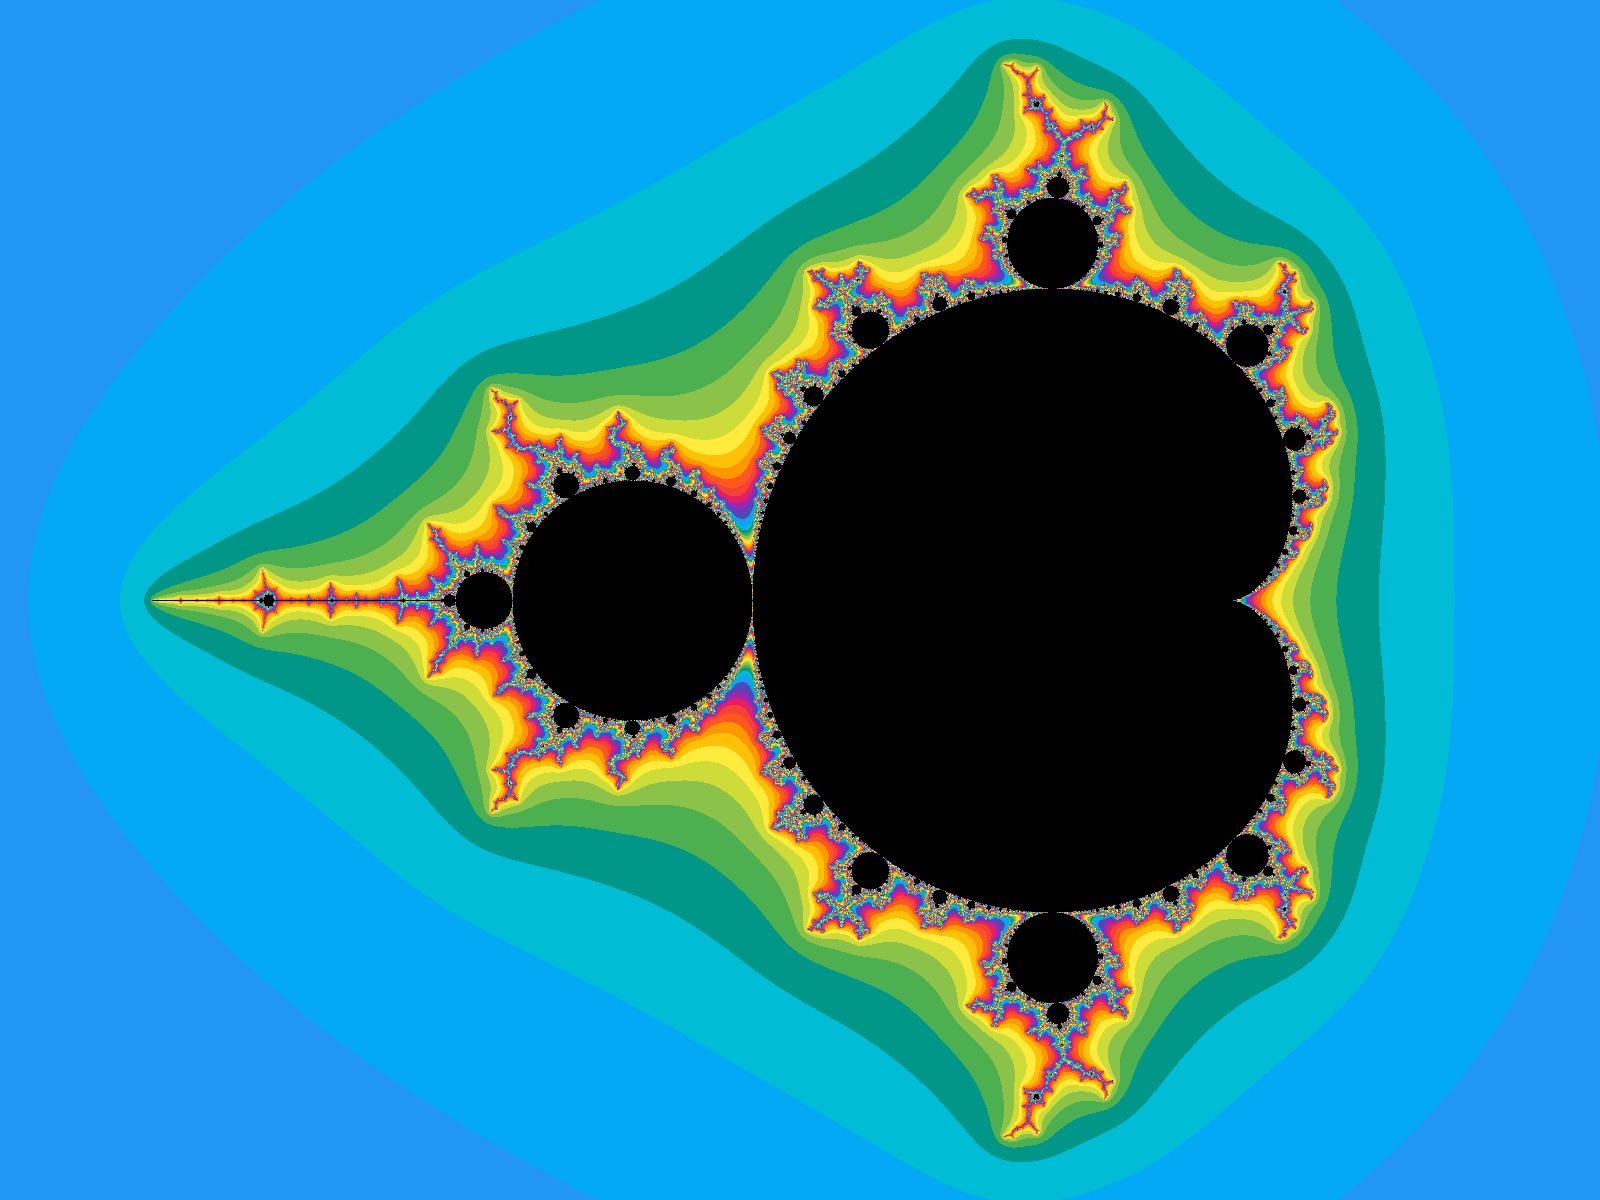
\includegraphics[width=1.3\textwidth]{data/83.png}}
  }\end{column}
\end{uloha}


Pekné, ale stále trochu vadí, že prechody medzi farbami sú náhle. Chcel by som, aby
zafarbenie bolo plynulé. Na to treba vyriešiť dva problémy: ako vyrobiť ''paletu'', v ktorej
sú plynulé prechody a potom ako nahradiť počet iterácií niečím, čo sa plynulejšie mení.


Prvý problém vyriešime pomocou {\em interpolácie} farieb. Interpolácia je vlastne\indexItem{Alg}{interpolácia}
proporcionálne zmie\-ša\-va\-nie: ak mám čísla $a$ a $b$, a parameter $t$, ktorý vyjadruje
časť (t.j. $0\le t\le1$), môžem ich zmiešať tak, že zoberiem $t$-tinu z $a$ a
zvyšok (t.j. $1-t$) doplním z $b$: dostanem $ta+(1-t)b$. Ak je $t=0$, mám $b$, ak je
$t=1$, mám $a$ a ak sa $t$ plynule mení, aj výsledná hodnota plynule prechádza z $b$ do $a$
(pre $t=1/2$ mám priemer). Pre dve farby môžeme urobiť to isté: nezávisle interploáciu
v červenej, zelenej a modrej zložke\footnote{%
Len pre informáciu: existuje veľa rôznych farebných modelov, ktoré tiež reprezentujú farbu
pomocou niekoľkých (spravidla) troch čísel, ale tie čisla nie sú ''červená'', ''zelená'', 
''modrá'',
ale napr. ''farba'',''sýtosť'',''jas'' a pod. Práve RGB model nie je veľmi 
vhodný na interpoláciu po zložkách, na to sú lepšie kolorimetrické modely ako XYZ.
Ale na naše účely to stačí v pohode.
}. Spravme triedu \vb{Gradient}, ktorá bude obsahovať pole zlomových bodov. Zlomový\indexItem{Alg}{farebný gradient}
bod má pozíciu (z rozsahu 0\ldots1) a farbu. \vb{Gradient} potom
pre dané \vb{x} zistí\footnote{%
  napr. binárnym vyhľadávaním, aj keď pre málo zlomových bodov je 
  binárne vyhľadávanie overkill},
  bedzi ktorými zlomovými bodmi sa nachádza, a vráti príslušnú interpoláciu.
  Gradient s troma zlomovými bodmi vyzerá napríklad takto:
  

\centerline{\begin{tikzpicture}[xscale=5,yscale=2.2,
  every text node part/.style={align=center}]
  \def\step{0.1}
  \def\mark(#1)#2#3{%
    \draw[->,shorten <= 1ex , shorten >= 1ex] (#1+0.5*\step,1.5) 
    node[anchor=south]{$t=#2$\\ \textcolor{magenta}{\vb{\##3}}}
    -- (#1+0.5*\step,1);
    }
  \foreach \t in {0,\step,...,1} {
    \pgfmathsetmacro{\r}{0.1*\t+ 0.4*(1-\t)}
    \pgfmathsetmacro{\g}{0.2*\t+ 0.8*(1-\t)}
    \pgfmathsetmacro{\b}{0.8*\t+ 0.2*(1-\t)}
    \definecolor{myfill}{rgb}{\r,\g,\b}
    \filldraw[fill=myfill](\t,0) rectangle (\t+\step,1);
  }
  \begin{scope}[shift={(1,0)}]
  \foreach \t in {0,\step,...,2} {
    \pgfmathsetmacro{\ts}{0.5*\t}
    \pgfmathsetmacro{\r}{1*\ts+ 0.1*(1-\ts)}
    \pgfmathsetmacro{\g}{0.35*\ts+ 0.2*(1-\ts)}
    \pgfmathsetmacro{\b}{0.2*\ts+ 0.8*(1-\ts)}
    \definecolor{myfill}{rgb}{\r,\g,\b}
    \filldraw[fill=myfill](\t,0) rectangle (\t+\step,1);
  }
  \end{scope}
  \mark(0){0}{66cc33}
  \mark(1){0.33}{1a33cc}
  \mark(3-\step){1}{ff5933}

  \draw[->,shorten <= 1ex , shorten >= 1ex] (2+0.5*\step,-0.5)
  node [anchor=north]{\vb{x}}-- (2+0.5*\step,0);
\end{tikzpicture}}


S pomocou knižnice \vb{cmath}, v ktorej je funkcia \vb{fmod}: zvyšok\indexItem{Prg}{\vb{fmod}}
po delení, ale pre desatinné čísla (t.j. \prg!fmod(t,1)! je desatinná
časť z \vb{t}) môže implementácia vyzerať napr. takto:


\begin{lstlisting}
struct Stop {
  double t;
  RGBA f;
};

struct Gradient {
  vector<Stop> stops;

  Gradient(const vector<Stop>& _stops) { stops = _stops; }

  RGBA operator()(double t) {
    t=fmod(t,1);
    RGBA x;
    auto it = lower_bound(stops.begin(), stops.end(), Stop{t, {}},
                          [](Stop a, Stop b) { return a.t < b.t; });

    if (it == stops.begin()) return stops[0].f;
    RGBA a = (it)->f, b = (it - 1)->f;
    t = (t - (it - 1)->t) / (it->t - (it - 1)->t);

    x.r = (Byte)(t * a.r + (1 - t) * b.r);
    x.g = (Byte)(t * a.g + (1 - t) * b.g);
    x.b = (Byte)(t * a.b + (1 - t) * b.b);
    return x;
  }
};
\end{lstlisting}


Druhý problém je, akú hodnotu použiť namiesto počtu iterácií, aby sa menila spojitejšie.
Po troche hrania sa mi osvedčilo toto: pre každý pixel si zapamätám počet iterácií a
jeho veľkosť v čase keď prekročil hranicu (kvôli väčšej plynulosti beriem logaritmus
z veľkosti; v knižnici \vb{cmath} je na to funkcia \vb{log}). Potom, keď som mal
hotový celý obrázok, tak som zistil všetky počty iterácií, ktoré sa vyskytli a pre každý počet iterácií našiel maximálnu a minimálnu hodnotu
veľkosti. Každý pixel potom dostal okrem počtu iterácií aj desatinnú časť, ktorá závisela od
jeho veľkosti (relatívne k maximálnej a minimálnej veľkosti pre tento počet iterácií).


\begin{column}{0.45}
\vskip 0pt
\begin{lstlisting}
Gradient g(
{{0.0, RGBA(0, 7, 100)},
{0.16, RGBA(32, 107, 203)},
{0.42, RGBA(237, 255, 255)},
{0.6425, RGBA(255, 170, 0)},
{0.8575, RGBA(0, 2, 0)},
{1.0, RGBA(0, 7, 100)}});
\end{lstlisting}
\end{column}
\hfill
\begin{column}{0.45}
\vskip 0pt
\centerline{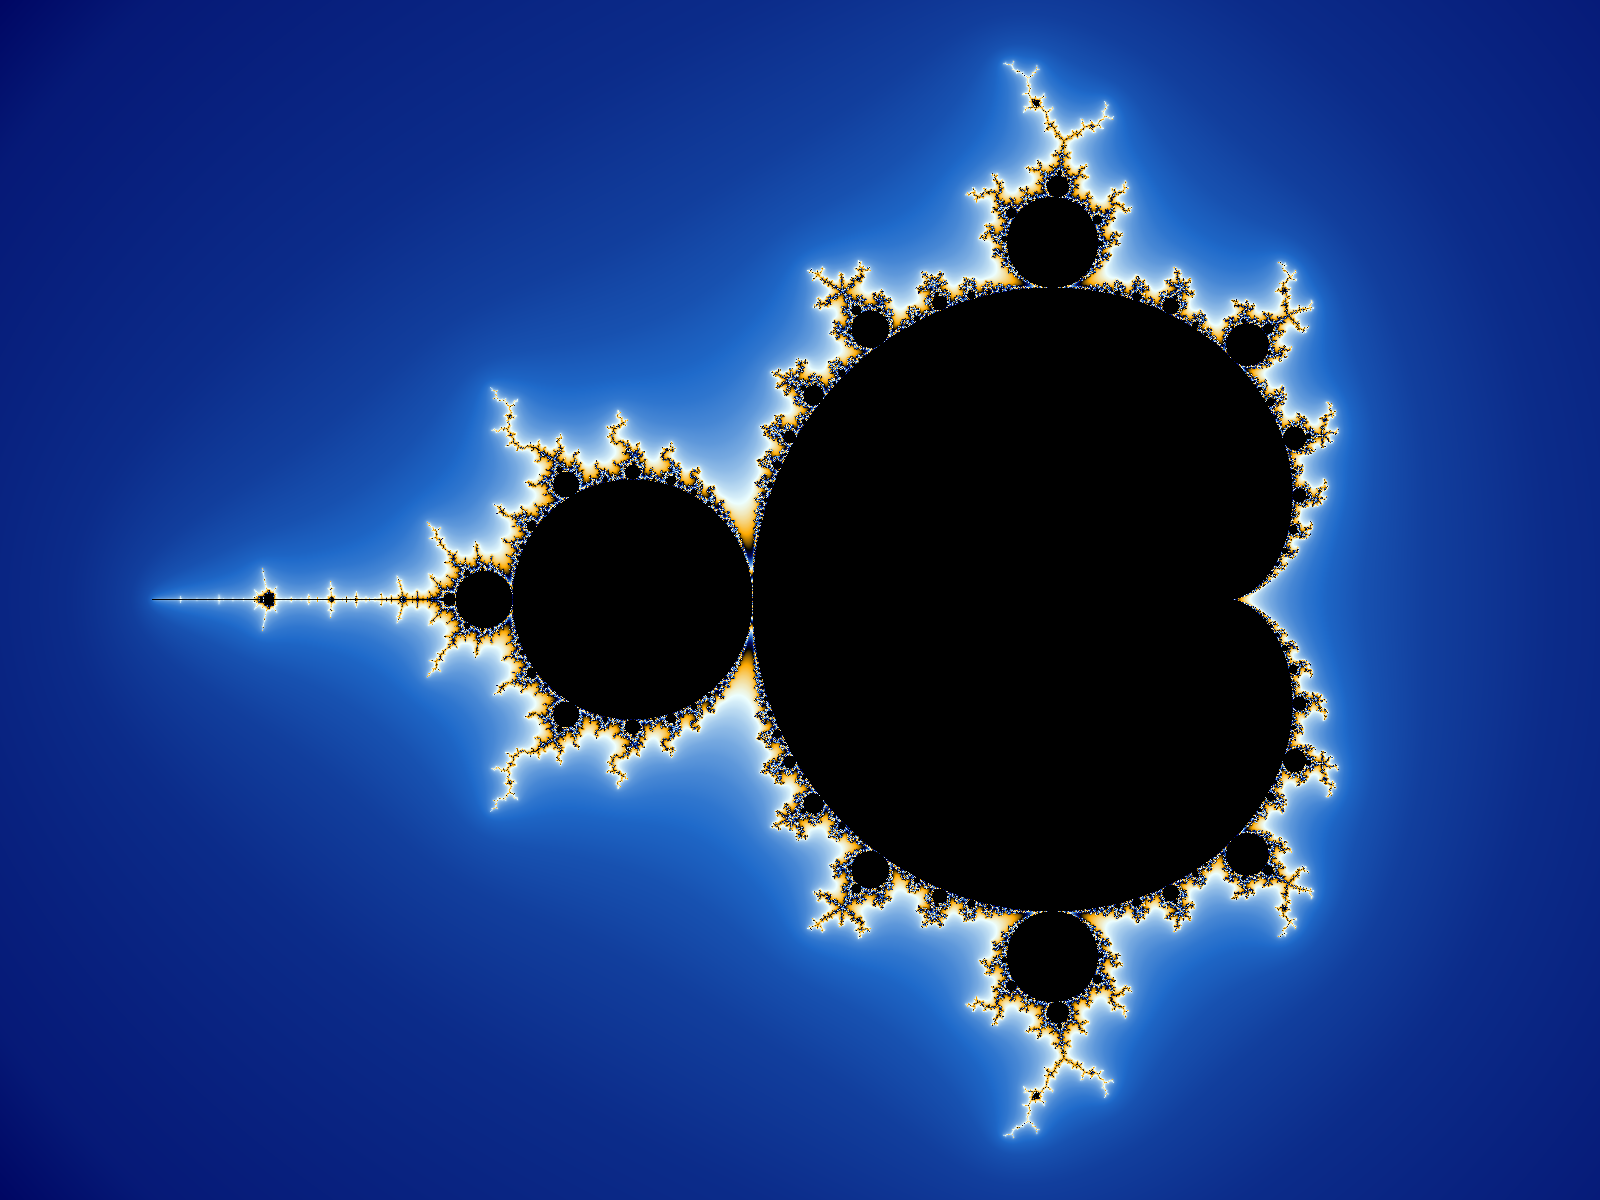
\includegraphics[width=1.1\textwidth]{data/mb.png}}
\end{column}


\begin{column}{0.45}
\vskip 0pt
\centerline{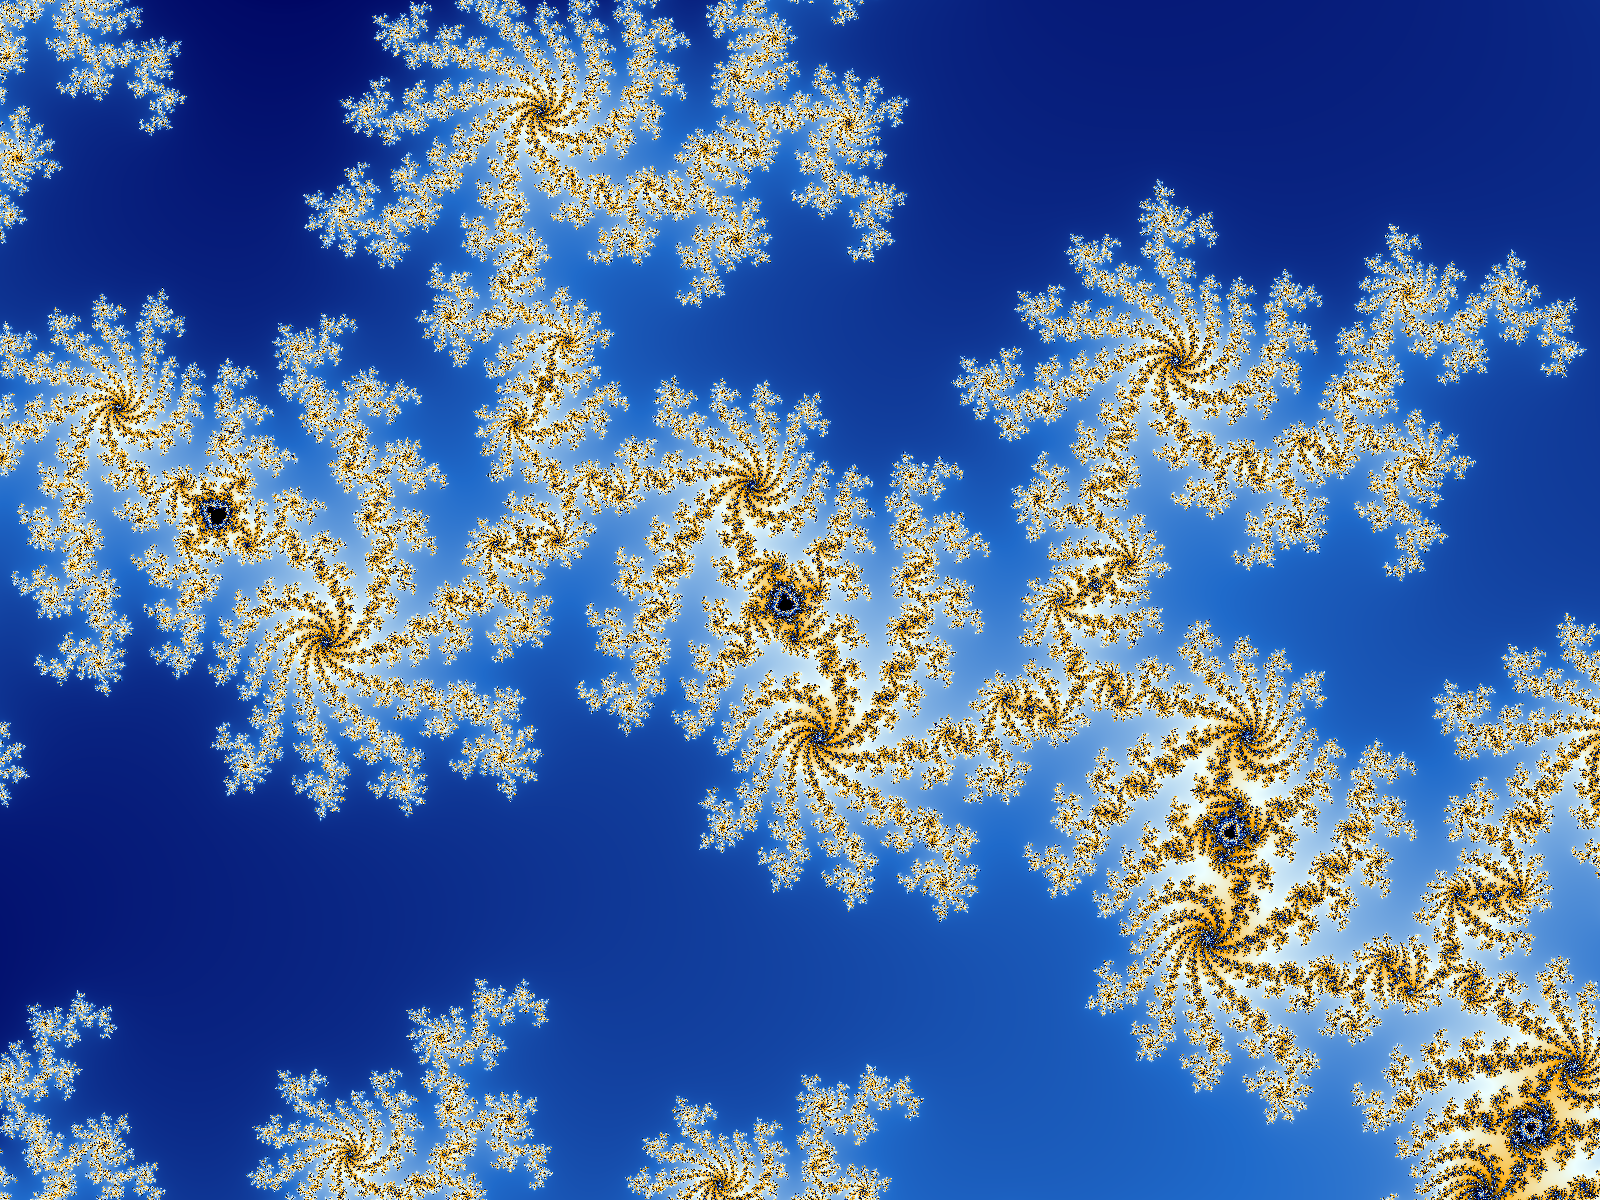
\includegraphics[width=1.1\textwidth]{data/mb1.png}}
\centerline{stred $(-0.6928223,0.3282697)$}
\centerline{$m=508.9334$}
\end{column}
\hfill
\begin{column}{0.45}
\vskip 0pt
\centerline{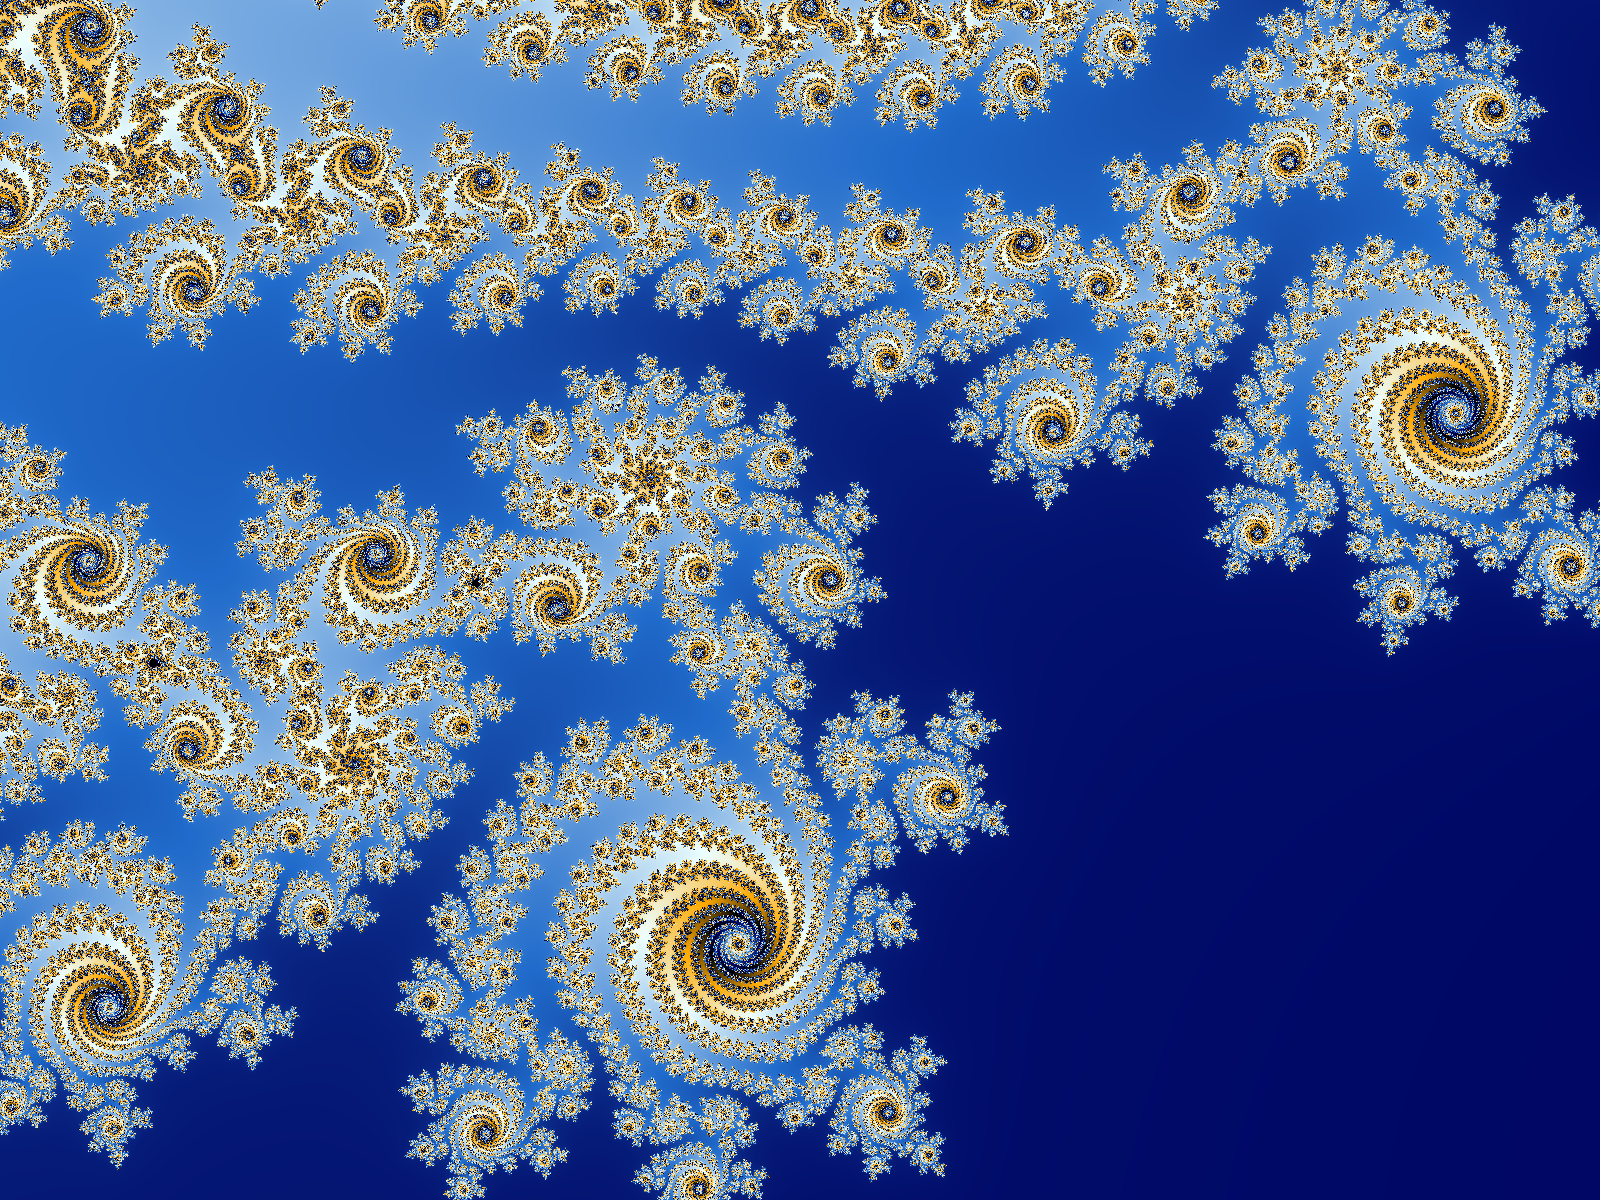
\includegraphics[width=1.1\textwidth]{data/mb2.png}}
\centerline{stred $(-0.59990625,-0.4290703125)$}
\centerline{$m=1500$}
\end{column}


\begin{column}{0.45}
\vskip 0pt
\centerline{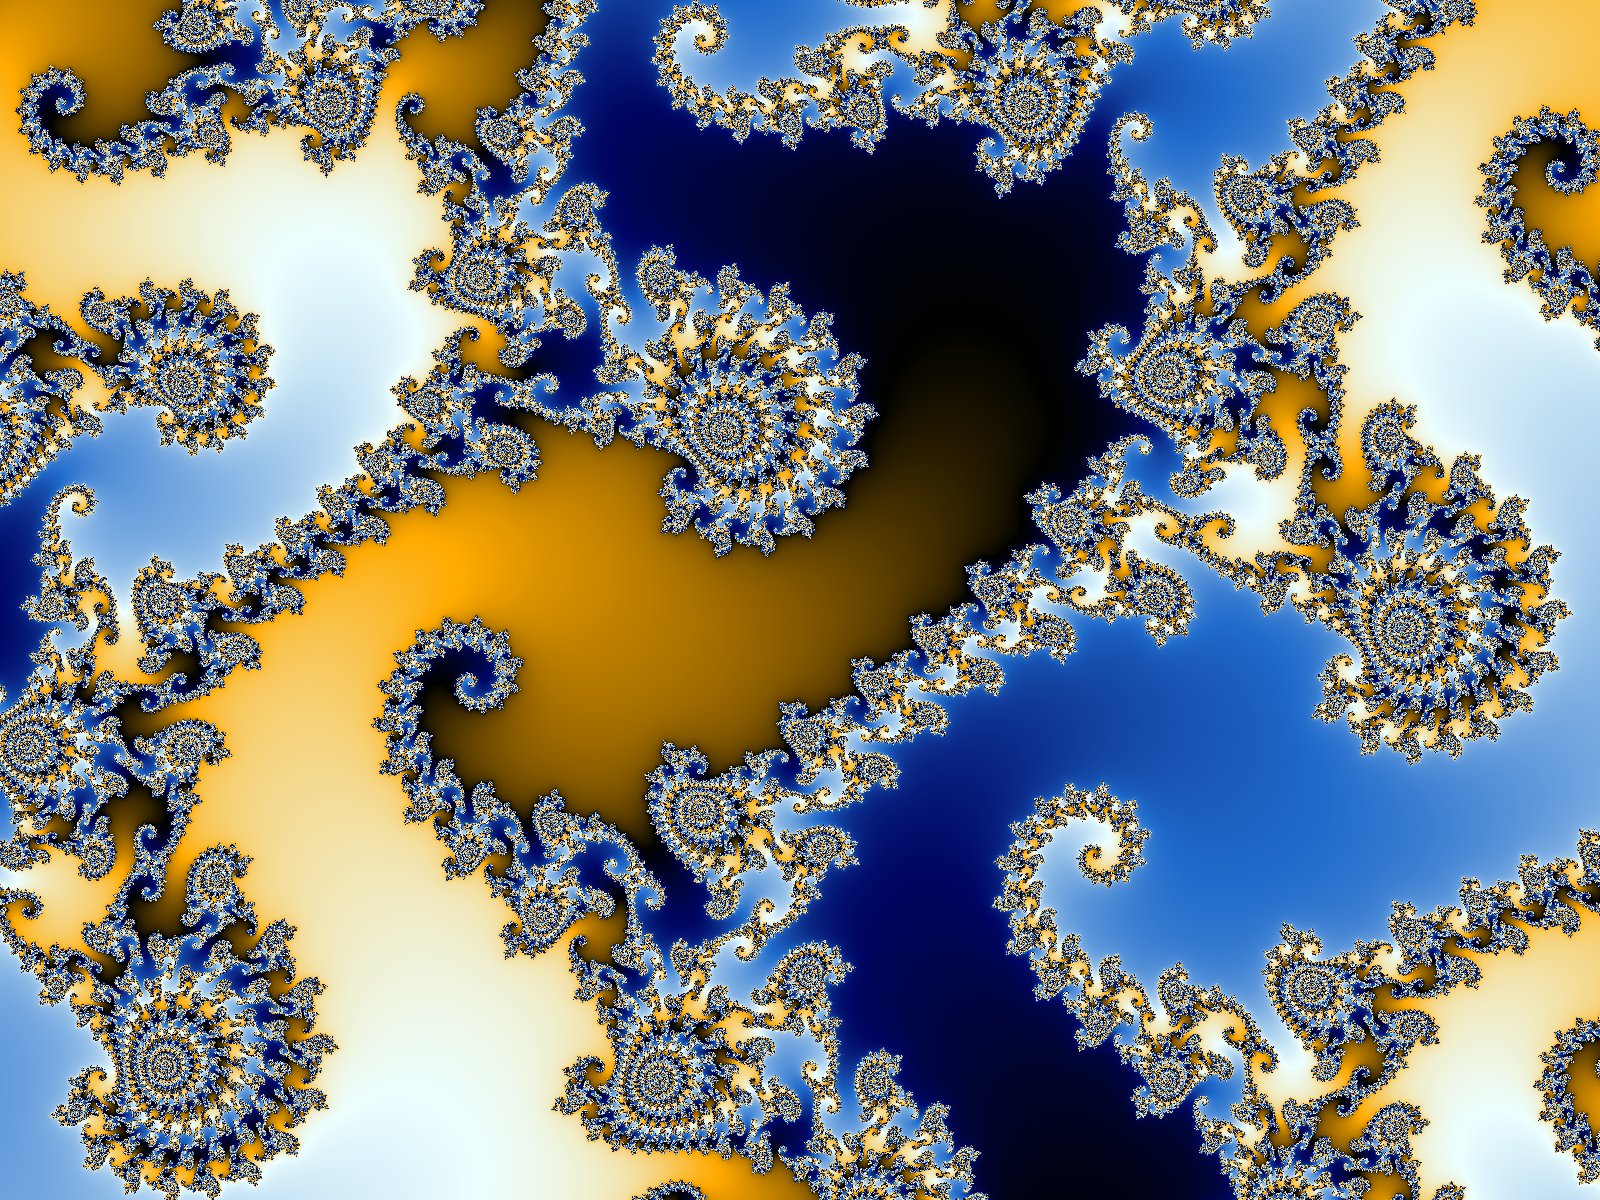
\includegraphics[width=1.1\textwidth]{data/mb3.png}}
\centerline{stred $(-0.743643887035763,0.13182590421259918)$}
\centerline{$m=4.3e14$}
\end{column}
\hfill
\begin{column}{0.45}
\vskip 0pt
\centerline{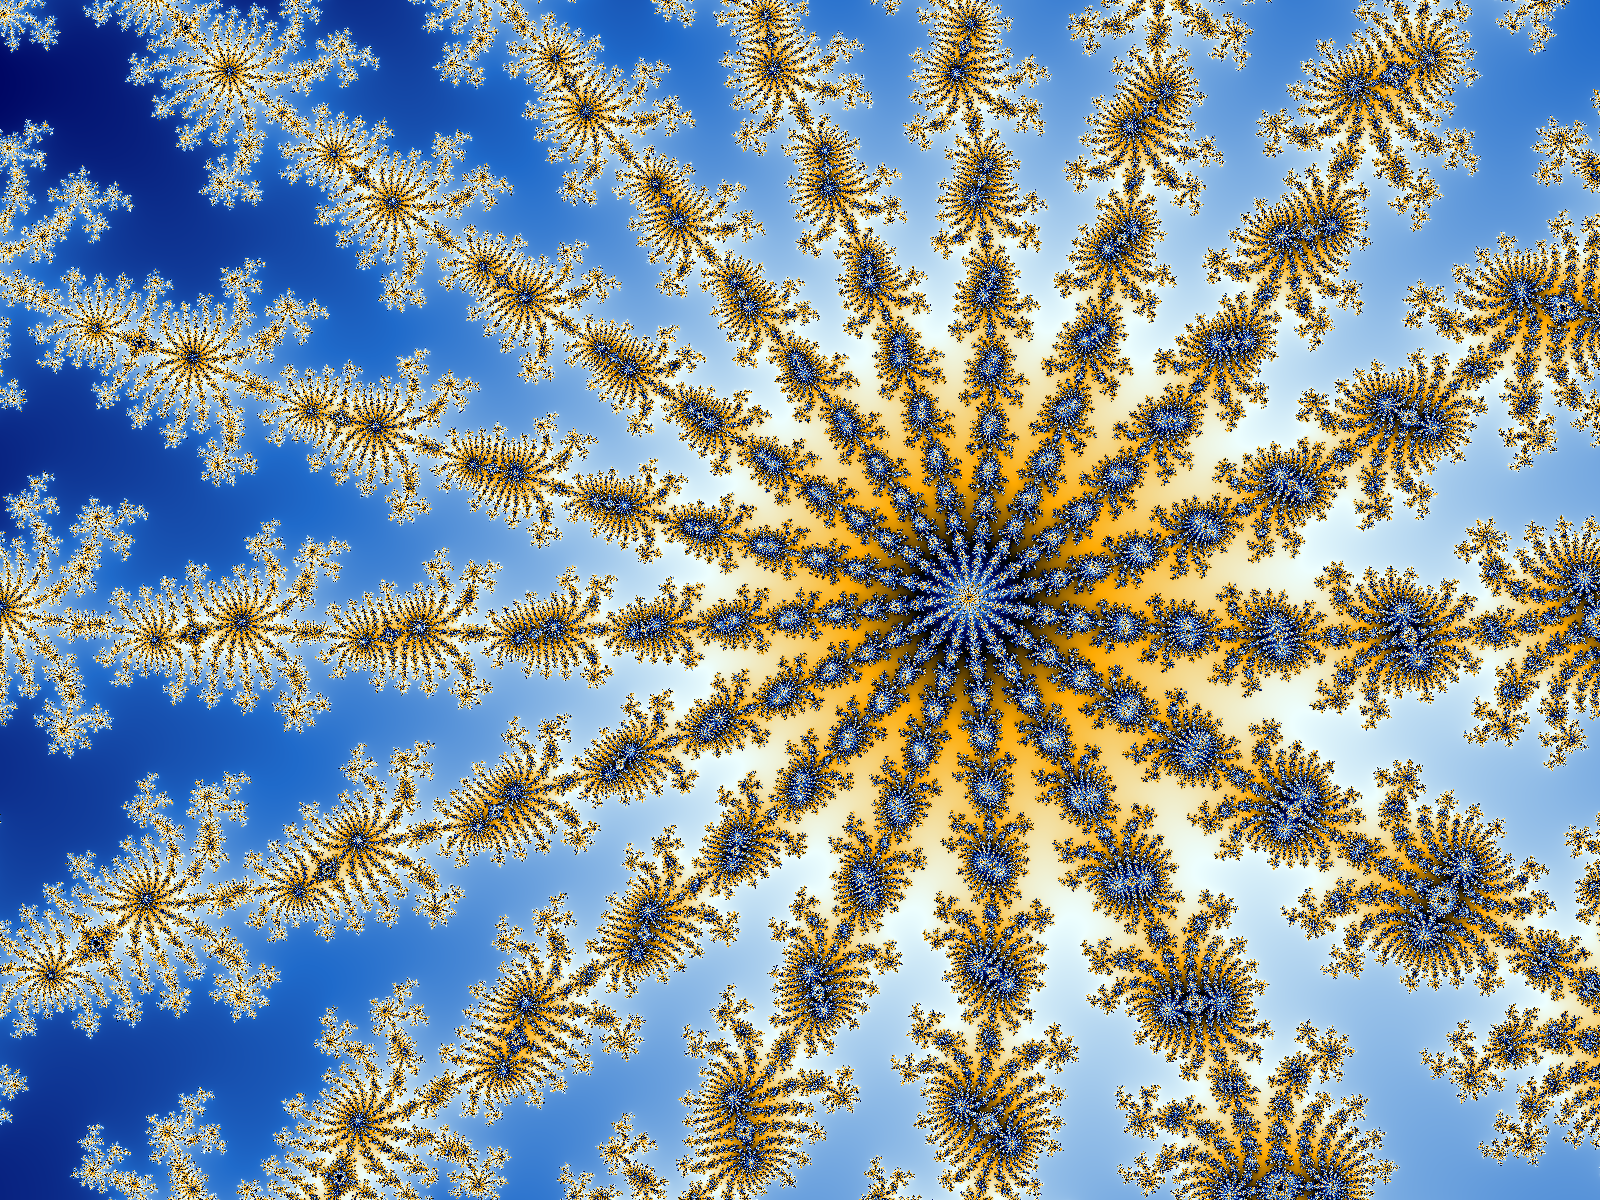
\includegraphics[width=1.1\textwidth]{data/mb4.png}}
\centerline{stred $(-0.65550685,0.3783525)$ }
\centerline{$m=236.2$}
\end{column}

\begin{uloha}
  Pohraj sa s Mandelbrotovou množinou.
\end{uloha}


\chapter{Vyhľadávacie stromy: \vb{<set>} a \vb{<map>} v STL}
\label{sect:stromy}

Pri farbení Mandelbrotovej množiny v závere minulej kapitoly som robil túto vec:
''{\em \ldots pre každý počet iterácií } [som] {\em našiel maximálnu a minimálnu hodnotu
\ldots}''. Ak si sa pozrel do môjho programu, tak si videl, že som trochu cheatoval
a použil som typ \prg!map! z STL, o ktorom som ti doteraz nehovoril. Ale v tejto
kapitole to chcem napraviť. Začnime jednoduchou rozcvičkou:

\begin{uloha}
  Na vstupe je číslo $n$. A potom postupnosť príkazov. Každý príkaz je tvaru
  \vb{! x} alebo \vb{? x} a posledný príkaz je \vb{\#}. 
  Predpokladajme, že máme $n$ žiaroviek očíslovaných $1,\ldots,n$, 
  ktoré su na začiatku vypnuté. Príkaz \vb{! x} znamená, že sme prepli žiarovku
  číslo $x$ (ak bola vypnutá, bude zapnutá a naopak). Pre každý príkaz \vb{? x}
  treba vypísať, \vb{svieti} alebo \vb{nesvieti} podľa toho, v akom stave je práve žiarovka
  číslo $x$.
\end{uloha}

Jednou z možností, ako túto úlohu vyriešiť, bolo urobiť si vektor $n$ hodnôt typu \prg!bool!
tak, že v \prg!a[i]! si budeme udržiavať stav $i$-tej
žiarovky. Predpokladajme teraz ale, že by žiarovky neboli očíslované $1$ až $n$, ale
že by mali iba výrobné čísla. Vstup by mohol vyzerať napríklad:\\

\begin{outputBox}
! 3736272
! 843984
? 3736272
! 84872634
! 72876
? 99
? 843984
#
\end{outputBox}

Problém je, že nevieme, aké výrobné čísla sa na vstupe objavia. Nemôžme si držať v pamäti 
pole pre všetky možné čísla, takže chceme mať zapamätané iba tie žiarovky, ktoré sme 
už videli. Teraz ale stoja proti sebe dve veci: ak chcem nájsť stav žiarovky s číslom 
\vb{id}, hodilo by sa mi mať žiarovky utriedené podľa čísla: mohol by som použiť
binárne vyhľadávanie, aby som zistil, či \vb{id} svieti. Ak ich utriedené nemám,
musím zakaždým prejsť všetky, čo trvá dlho. Na druhej strane, keď sa  objaví nová
žiarovka, ľahko ju pridám na koniec, ale potom nebudú utriedené. Musel by som 
všetky žiarovky v poli poposúvať, čo zase trvá dlho. 
Riešenie je namiesto poľa (vektora) použiť dátovú štruktúru, ktorá nemá všetky dáta
v jednom kuse pamäte, ale vo viacerých, ktoré na seba navzájom ukazujú pointrami. Tým
sa bude dať docieliť, že pri vkladaní nového prvku
bude namiesto posúvania všetkých hodnôt stačiť presmerovať
zopár pointrov. 

 Aby som ti ukázal, ako také štruktúry fungujú, začnime s jednoduchším príkladom
a k žiarovkám sa vrátime na konci kapitoly.

\begin{uloha}
  Úradník má kartotéku, kde má uložené spisy očíslované $0,1,\ldots,n-1$ (na začiatku
  v tomto poradí).
  Keď potrebuje nájsť spis $i$, začne prehľadávať zaradom od začiatku kartotéky
  a vždy prečíta číslo spisu, až kým nenájde ten s číslom $i$. Ten potom použije a 
  uloží na začiatok kartotéky. Napíš program, ktorý má na vstupe čísla $n, m$ a potom
  $m$ čísel spisov (medzi 0 a $n-1$). Pre každé číslo spisu vypíš riadok, v ktorom 
  sú čísla spisov, ktoré úradník prečítal pri hľadaní. Napríklad

  
  \begin{column}{0.45}
  \begin{outputBox}
6 4
5
3
4
1
\end{outputBox}
\end{column}
\begin{column}{0.45}
\begin{outputBox}
0 1 2 3 4 nasiel som 5!
5 0 1 2 nasiel som 3!
3 5 0 1 2 nasiel som 4!
4 3 5 0 nasiel som 1!

\end{outputBox}
\end{column}
\end{uloha}


Na riešenie použijeme dátovú štruktúru {\em spájaný zoznam} ({\em linked list}).\indexItem{Alg}{spájaný zoznam}
Každý prvok zoznamu je uložený v samostatne alokovanej pamäti a má pointer
na nasledujúci prvok. Spravíme si typ

\begin{lstlisting}
struct Node {
  int val;
  Node *nxt;
  Node(int _val = -1, Node *_nxt = nullptr) {
    val = _val;
    nxt = _nxt;
  }
};
\end{lstlisting}

v ktorom bude jeden prvok zoznamu\footnote{%
  Možno ťa zaskočilo, že súčasťou typu \vb{Node} je premenná \vb{nxt}, ktorá
  je pointer na typ \vb{Node}. Nie je v tom ale nič zvláštne -- pointer je iba číslo
  adresy v pamäti. Typ pointra (v našom prípade \vb{Node *}) iba hovorí kompilátoru,
  že na adrese uloženej v premennej \vb{nxt} má očakávať premennú typu \vb{Node}.
  Pretože všetky pointre sú rovnako dlhé, kompilátoru nevadí, že typ \vb{Node} zatiaľ nie 
  je pripravený, stačí mu vedieť, koľko miesta treba v pamäti vyhradzovať.
  }. V programe budeme mať zoznam zapamätaný iba pointrom
na jeho začiatok \prg!Node *head;! Zoznam \vb{[0 1 2 3 4 5]} by v pamäti vyzeral takto:\\
    

    \def\llnode(#1,#2)[#3]#4{
      \begin{scope}[shift={(#1,#2)}]
        \draw [\nodecolor, rounded corners=2pt] (-0.5,-0.5) rectangle (0.5,0.5)
        (-0.5,0) -- (0.5,0)
        (-0.5,0.25) node [anchor=west]{{\robotomono val:}}
        (0.3,0.25) node[anchor=center]{{\robotomono #4}}
        (-0.5,-0.25) node [anchor=west]{{\robotomono nxt:}}
        (0.3,-0.25) node[anchor=center] {$\bullet$};
        \coordinate (n#3) at (0.3,-0.25);
        \coordinate (b#3) at (-0.5,0.25);
      \end{scope}
    }

    \def\head(#1,#2){
      \node[\nodecolor,anchor=east] (head) at (#1,#2) {\vb{head:}};
      \node[\nodecolor,right = 0mm of head, ] (headbullet) {$\bullet$};
    }


%\tikzset{external/force remake}
\centerline{
  \begin{tikzpicture}[xscale=1.4*0.8,yscale=0.8]
    {\small
    \def\nodecolor{cyan!50!blue}
    \foreach \v/\c[count =\i] in {0/A, 1/B, 2/C, 3/D, 4/E, 5/F} {
      \llnode(1.5*\i,0.5)[\c]{\v}
    }
    \foreach \x/\y in {A/B, B/C, C/D, D/E, E/F} {
    \draw[->,\nodecolor,shorten >= 0.15ex](n\x) to[out=0, in=180] (b\y);
    }
    \head(0,0);
    \draw[\nodecolor,->, shorten >= 0.15ex] (headbullet) to[out=0,in=180] (bA);
    \draw[\nodecolor,-|] (nF) to [out=0,in=90] ++(0.5,-0.5);
    }
  \end{tikzpicture}
}



Vyrobíme ho jednoducho:

\begin{lstlisting}
head = nullptr;
for (int i = 0; i < n; i++)
  head = new Node(n - 1 - i, head);
\end{lstlisting}

V cykle vždy pri vyhodnocovaní pravej strany priradenia 
vyrobíme novú premennú typu \vb{Node}, v ktorej nastavíme \vb{val}
na správnu hodnotu a \vb{nxt} na rovnaké miesto, ako práve ukazuje \vb{head}.
V priradení potom nastavíme \vb{head}, aby ukazoval na túto novú premennú.\\


\centerline{

  \begin{tikzpicture}[xscale=1.4*0.8, yscale=0.8]
    {\small
    \def\nodecolor{cyan!50!blue}
    \foreach \v/\c[count =\i] in {4/A, 5/B} {
      \llnode(0.8+1.5*\i,0.5)[\c]{\v}
    }
    \foreach \x/\y in {A/B} {
    \draw[->,\nodecolor,shorten >= 0.15ex](n\x) to[out=0, in=180] (b\y);
    }
    \head(0,0);
    \draw[\nodecolor,->, shorten >= 0.15ex] (headbullet) to[out=0,in=180] (bA);
    \draw[\nodecolor,-|] (nB) to [out=0,in=90] ++(0.5,-0.5);
    
    \def\nodecolor{orange!80!black}
    \llnode(0.5,1.2)[C]{3}
    \draw[\nodecolor,->, shorten >= 0.15ex] (nC) to [out=0,in=90] ($(bA)+(0.5,0.25)$);
    }  
  \end{tikzpicture}
  \hfill
  \begin{tikzpicture}[xscale=1.4*0.8,yscale=0.8]
    {\small
    \def\nodecolor{cyan!50!blue}
    \foreach \v/\c[count =\i] in {4/A, 5/B} {
      \llnode(1.5+1.5*\i,0.5)[\c]{\v}
    }
    \foreach \x/\y in {A/B} {
    \draw[->,\nodecolor,shorten >= 0.15ex](n\x) to[out=0, in=180] (b\y);
    }
    \head(0,0);
    
    \llnode(1.5,1.2)[C]{3}
    \draw[\nodecolor,->, shorten >= 0.15ex] (nC) to [out=0,in=90] ($(bA)+(0.5,0.25)$);
    
    \draw[\nodecolor,-|] (nB) to [out=0,in=90] ++(0.5,-0.5);
    
    \def\nodecolor{orange!80!black}
    \draw[\nodecolor,->, shorten >= 0.15ex] (headbullet) to[out=0,in=180] (bC);
   }
  \end{tikzpicture}
}


Povedzme, že už máme vyrobený zoznam a máme v ňom nájsť hodnotu \vb{x}\footnote{%
a sme si istí, že \vb{x} sa v zozname nachádza, takže nemusíme kontrolovať, či sme
prišli na koniec zoznamu}. Spravím si premennú \vb{Node *p = heaad;}, s ktorou pôjdem
po zozname

\begin{lstlisting}
while (p->val != x) p = p->nxt;
\end{lstlisting}

Teraz budem v situácii, že \vb{p} ukazuje na hľadaný prvok:


\centerline{
  \begin{tikzpicture}[xscale=1.4*0.8,yscale=0.8]
    {\small
    \def\nodecolor{cyan!50!blue}
    \foreach \v/\c[count =\i] in {0/A, 1/B, 2/C, 3/D, 4/E, 5/F} {
      \llnode(1.5*\i,0.5)[\c]{\v}
    }
    \foreach \x/\y in {A/B, B/C, C/D, D/E, E/F} {
    \draw[->,\nodecolor,shorten >= 0.15ex](n\x) to[out=0, in=180] (b\y);
    }
    \head(0,0);
    \draw[\nodecolor,->, shorten >= 0.15ex] (headbullet) to[out=0,in=180] (bA);
    \draw[\nodecolor,-|] (nF) to [out=0,in=90] ++(0.5,-0.5);
    
    \def\nodecolor{orange!80!black}
    \draw[\nodecolor,->, shorten >= 0.15ex ] (4*1.5,1.5) node[anchor=south]{\vb{p}} 
    -- ++(0,-0.5);
    }
  \end{tikzpicture}
}

 Ako presunúť nájdený prvok na začiatok zoznamu? Najprv ho vypojím a potom napojím
na začiatok. Na vypojenie potrebujem nastaviť \vb{nxt} v predchodcovi na \vb{p->nxt}.
Preto si upravím cyklus, ktorým prechádzam zoznam tak, aby som našiel aj predchodcu \vb{p}:

\begin{lstlisting}
Node *p = head, *prev = nullptr;
while (p->val != x) {
  prev = p;
  p = p->nxt;
}
if (prev != nullptr) 
  prev->nxt = p->nxt;
\end{lstlisting}


\centerline{
  \begin{tikzpicture}[xscale=1.4*0.8,yscale=0.8]
    {\small
    \def\nodecolor{cyan!50!blue}
    \foreach \v/\c[count =\i] in {0/A, 1/B, 2/C, 3/D, 4/E, 5/F} {
      \llnode(1.5*\i,0.5)[\c]{\v}
    }
    \foreach \x/\y in {A/B, B/C, D/E, E/F} {
    \draw[->,\nodecolor,shorten >= 0.15ex](n\x) to[out=0, in=180] (b\y);
    }
    \head(0,0);
    \draw[\nodecolor,->, shorten >= 0.15ex] (headbullet) to[out=0,in=180] (bA);
    \draw[\nodecolor,-|] (nF) to [out=0,in=90] ++(0.5,-0.5);
    
    \def\nodecolor{orange!80!black}
    \draw[\nodecolor,->, shorten >= 0.15ex ] (4*1.5,1.5) node[anchor=south]{\vb{p}} 
    -- ++(0,-0.5);
    
    \def\nodecolor{green!50!black}
    \draw[\nodecolor,->, shorten >= 0.15ex ] (3*1.5,1.5) node[anchor=south]{\vb{prev}} 
    -- ++(0,-0.5);
     
     \draw[\nodecolor,->, shorten <= 0.5ex, shorten >= 0.15ex ] (nC) to [out=-80,in=270]
     ($(bE)+(0.5,-0.75)$);
 

    }
  \end{tikzpicture}
}


Teraz môžem presunúť \vb{p} na začiatok podobne, ako pri vytváraní zoznamu:

\begin{lstlisting}
p->nxt = head;
head = p;
\end{lstlisting}

 Celé riešenie potom vyzerá takto:

\begin{lstlisting}
int main() {
  int n, m;
  cin >> n >> m;
  Node *head = nullptr;
  for (int i = 0; i < n; i++)
    head = new Node(n - 1 - i, head);
  while (m > 0) {
    m--;
    int x;
    cin >> x;
    Node *p = head, *prev = nullptr;
    while (p->val != x) {
      cout << p->val << " ";
      prev = p;
      p = p->nxt;
    }
    cout<<"nasiel som "<<x<<"!"<<endl;
    if (prev != nullptr) {
      prev->nxt = p->nxt;
      p->nxt = head;
      head = p;
    }
  }
}
\end{lstlisting}
%\tikzset{external/force remake=false}

\begin{uloha}
  Pri riešení úlohy~\ref{uloha:mergesort} (MergeSort) v kapitole~\ref{sect:binarysearch}
  sme v operácii {\em merge}
  vždy prechádzali dve polia a výsledok kopírovali do tretieho. Napíš program na 
  triedenie algoritmom {\em MergeSort}, ktorý používa spájané zoznamy (funkcia
  \vb{sort} dostane ako parameter začiatok zoznamu) a nekopíruje
  dáta.
\end{uloha}


Spájaný zoznam\footnote{%
  Spájaný zoznam sa dosť často hodí, takže v STL je naprogramovaný v knižnici 
  \prg!<forward_list>!. Takže napr. \prg!forward_list<int> a;! 
  bude spájaný zoznam celých čísel. \prg!a! poskytuje iterátor podobne ako \prg!vector!,
  ale tento sa dá iba inkrementovať. Napr. 
  \prg~for(auto it = a.begin(); it != a.end() ; it++) cout << (*it) << endl;~
  vypíše prvky zo zoznamu. Na pridávanie a mazanie prvkov v zozname slúžia
  funkcie \prg!insert_after! a \prg!erase_after!, ktoré ako prvý parameter dostanú 
  iterátor, takže napr. \prg!insert_after(it,4)! vloží za prvok zoznamu, na ktorý ukazuje
  \prg!it!, nový uzol s prvkom $4$ a \prg!erase_after(it)! zmaže nasledujúci uzol.
  Na pridanie a zmazanie prvého prvku slúžia funkcie \prg!push_front(x)! a 
  \prg!pop_front()!.
  Pretože zoznam pracuje s pointermi na uzly, iterátory sa, na rozdiel od vektorov
  nikdy nezneplatnia (okrem prípadu, keď sa uzol vymaže).

  Podobná trieda ako \prg!<forward_list>! je \prg!<list>!. Rozdiel je v tom, že každý
  uzol si okrem pointra \prg!nxt! pamätá aj pointer \prg!prev! na predchádzajúci prvok.
  To znamená, že iterátory sa dajú aj dekrementovať, ale celý zoznam zaberá viac pamäte.
  Namiesto \prg!insert_after! a \prg!erase_after! má podobné funckie \prg!insert(it,x)! a
  \prg!erase(it)!, ktoré ale vkladajú prvok pred zadaný iterátor (takže vložiť prvok na 
  koniec zoznamu \prg!z! sa dá pomocou \prg!insert(z.end(),x)!.
}a pole sú v istom zmysle opakom jeden druhého: v poli sa dá jednoducho prejsť
na hociktorý prvok, ale zle sa preusporiadava, lebo prvky treba kopírovať. V spájanom zozname
sa zle prechádza na konkrétny prvok, lebo treba prejsť celý zoznam, ale dobre sa
preusporiadava, lebo stačí poprehadzovať pointre. Skúsme spojiť dobré vlastnosti z oboch.
Binárne vyhľadávanie v usporiadanom poli\footnote{%
  nateraz nás bude zaujímať pole, v ktorom sa hodnoty neopakujú -- 
  ako v príklade so žiarovkami} sa dá predstaviť ako rozhodovací strom:


\centerline{\begin{tikzpicture}[scale=0.8]
  \foreach \h[count=\i] in {1,2,1,3,1,2,1,4,1,2,1,3,1,2,1} {
    \draw[thin,gray,dotted] (\i+0.5,0.5) -- (\i+0.5,1.2+1.2*\h) coordinate (tmp-\i);
 
  }

  \foreach \i/\d  in {2/1,4/2,6/1,8/4,10/1,12/2,14/1} {
    \pgfmathtruncatemacro{\prev}{\i-\d}
    \pgfmathtruncatemacro{\next}{\i+\d}
    \draw[thick] (tmp-\prev) -- (tmp-\i) -- (tmp-\next);
  }

  \foreach \v [count=\i] in { 12,14,17,21,25,29,30,32,34,37, 38,41,42,45,49} {
    \filldraw[fill=yellow!20!white](\i,0) rectangle node[anchor=center]{\vb{\v}} (\i+1,1);

    \filldraw[fill=green!10!white] (tmp-\i) circle (2.2ex) node [anchor=center] {\vb{\v}};
  }
  
  \draw[thick,red] (11,0) rectangle (12,1);
  \foreach \i in {8,12,10,11} {
    \draw[very thick,red] (tmp-\i) circle(2.2ex);
  }

\end{tikzpicture}}


Keď chceme nájsť číslo $38$, najprv sa pozrieme do stredu, porovnám s číslon $32$, keďže
$38>32$, vydáme sa vpravo, porovnáme so $41$ atď. Našim cieľom teraz bude vyrobiť si takýto
rozhodovací strom v pamäti pomocou smerníkov. Keď sa pozrieš na obrázok, vidiš, že strom\indexItem{Alg}{binárny vyhľadávací strom}
sa skladá z krúžkov, ktoré budem volať {\em uzly} alebo {\em vrcholy}. V každom uzle 
je číslo, ktorému budem hovoriť {\em kľúč}. Najvyšší uzol v strede (na obrázku $32$) 
bude {\em koreň}, uzly naspodu budú {\em listy}. Z každého uzla okrem listu vedú 
dve čiary ({\em hrany}), ktoré vedú do koreňov menších stromov (tým hovoríme
{\em synovia} uzla). Najdlhšia vzdialenosť od koreňa do nejakého listu sa volá 
{\em hĺbka}. Základná vlastnosť,
ktorá umožňuje binárne vyhľadávanie, je to, že v celom strome aj vo všetkých podstromoch
platí: \cmd{keď si zoberiem hocijaký vrchol $v$, tak všetky kľúče v podstrome, ktorého koreň 
je ľavý syn $v$, sú menšie ako kľúč vo $v$
a všetky kľúče v podstrome, ktorého koreň je pravý syn $v$, sú zase väčšie}. 
Takýto strom budeme volať {\em binárny vyhľadávací strom}.
Spravme si takýto typ:

\begin{lstlisting}
struct Node {
  int key;
  Node *left, *right;

  Node(int _key = 0, Node *_l = nullptr, Node *_r = nullptr) {
    key = _key;
    left = _l;
    right = _r;
  }

  ~Node() {
    if (left != nullptr) delete left;
    if (right != nullptr) delete right;
  }

};
\end{lstlisting}


Vyzerá veľmi podobne ako pri spájanom zozname, len má dva pointre (na ľavého 
a pravého syna). 
Pridal som navyše deštruktor: ak sa ide z pamäti odstrániť
premenná typu \vb{Node} (či už pri volaní \prg!delete! alebo inak), najprv sa
zavolá deštruktor, ktorý sa pozrie, že existuje ľavý a/alebo pravý syn a ak áno,
rekurzívne ich zmaže (t.j. zavolá sa deštruktor ľavého syna, ktorý zavolá deštruktor
jeho synov atď), až sa zmaže celý strom. 


Ak máme utriedené pole prvkov, môžeme z neho vyrobiť strom napríklad takto:

\vbox{
  \begin{lstlisting}
Node *vyrob(vector<int> &a, int i, int j) {
  Node *res = new Node();
  if (i == j) {
    res->key = a[i];
  } else {
    int m = (i + j) / 2;
    res->key = a[m];
    if (i != m) res->left = vyrob(a, i, m - 1);
    if (m != j) res->right = vyrob(a, m + 1, j);
  }
  return res;
}
  \end{lstlisting}
}


Funkcia \vb{vyrob} má ako parametre referenciu na vektor a dva indexy \vb{i}
a \vb{j} a vyrobí strom, ktorý bude mať kľúče z úseku \prg!a[i]!\ldots\prg!a[j]!
(vrátane): zistí sa stredný prvok \vb{a[m]} a ak je ľavý alebo pravý úsek neprázdny,
rekurzívne sa zavolá \vb{vyrob} a novovytvorené podstromy sa priradia do pointrov
\vb{left} a \vb{right}. Ak mám napr. pole \vb{[10, 11, 14, 16, 20, 32, 42, 47, 50]}
a zvolám \prg!Node *root = vyrob(a, 0, a.size()-1);!, vyrobí sa v pamäti
takáto štruktúra z pointrov:

    \def\tnode(#1)[#2]#3{
      \begin{scope}[shift={(#1)}, xscale=1.3*0.7, yscale=0.7]
        \filldraw [\nodecolor, rounded corners=3pt, fill=white ] 
        (-0.5,-0.5) rectangle (0.5,0.5)
        (-0.5,0) -- (0.5,0)
        (0,0) -- (0,-0.5)
        (0,0.25) node [anchor=center]{\textcolor{magenta}{\vb{#3}}}
        (-0.25,-0.25) node[anchor=center] {\scriptsize {$\bullet$}}
        (0.25,-0.25) node[anchor=center] {{\scriptsize $\bullet$}}
        ;
        \coordinate (#2l) at (-0.25,-0.25);
        \coordinate (#2r) at (0.25,-0.25);
        \coordinate (#2) at (0,0.5);
        \coordinate (#2h) at (-0.5,0);
      \end{scope}
    }


\centerline{
  \begin{tikzpicture}[scale=0.8]
    {\small
    \def\nodecolor{cyan!50!blue}
    \foreach \h[count=\i] in {1,2,1,3,1,2,1,4,1,2,1,3,1,2,1} {
      \coordinate (tmp-\i) at (0.9*\i,0.15*\h*\h+0.8*\h) ;
    }

    \foreach \v/\c[count=\i] in {10/2, 11/4, 14/6, 16/7, 20/8, 32/10, 42/12, 47/14, 50/15} {
      \tnode(tmp-\c)[n\i]{\v}
    }

    
    \foreach \a/\b in {n2l/n1,n2r/n3,n3r/n4,n5l/n2,n5r/n7,n7l/n6,n7r/n8,n8r/n9} {
      \draw[\nodecolor,->,shorten >= 0.2ex] (\a) to[out=270,in=90] (\b);
    }
    \draw[\nodecolor,->,shorten >= 0.2ex, shorten <= 0.5ex ] ($(n5)+(0,0.5)$)
    node[anchor=south]{\vb{root}} -- (n5);
    }
  \end{tikzpicture}
}



Keď chceme zistiť, či sa nejaký kľúč v strome nachádza, stačí prechádzať stromom 
od koreňa (napr. \prg!root->find(42);!). 
Metóda \vb{find} vráti pointer na uzol s daným kľúčom,
alebo \prg!nullptr!, ak sa tam kľúč nenachádza. 

\begin{lstlisting}
struct Node {
  int key;
  Node *left, *right;
  Node(int _key = 0, Node *_l = nullptr, Node *_r = nullptr) {...}
  ~Node() {...}

  Node *find(int x) {
    if (x == key) return this;
    if (x < key && left != nullptr) return left->find(x);
    if (x > key && right != nullptr) return right->find(x);
    return nullptr;
  }
};
\end{lstlisting}


Teraz sme docielili, že v pamäti máme namiesto poľa prvky pospájané smerníkmi
a môžeme v nich vyhľadávať rovnako, ako pri binárnom vyhľadávaní v poli (teda
v logaritmickej zložitosti). Oproti binárnemu vyhľadávaniu v poli sme si ale pomohli v tom, že aj pridanie prvku má logaritmickú
zložitosť: jednoducho ideme po strome, ako keby sme vyhľadávali, a keď prídeme
na koniec, vyrobíme nový uzol. Metóoda \vb{insert} vráti \prg!true!, ak sa vrchol
v skutočnosti pridal a \prg!false!, ak už v strome bol:\\

\vbox{
\begin{lstlisting}
struct Node {
  int key;
  Node *left, *right;
  Node(int _key = 0, Node *_l = nullptr, Node *_r = nullptr) {...}
  ~Node() {...}
  Node *find(int x) {...}

  bool insert(int x) {
    if (x == key) return false;
    if (x < key && left != nullptr) return left->insert(x);
    if (x > key && right != nullptr) return right->insert(x);
    Node *nd = new Node(x);
    if (x < key) left = nd;
    else right = nd;
    return true;
  }

};
\end{lstlisting}
}

Zdá sa, že všetko funguje, a to je podozrivé. A naozaj. Keď začneš s jednoprvkovým
poľom \vb{[10]} a postupne voláš \vb{insert} pre $11, 14, 16, 20, 32, 42, 47, 50$,
v pamäti to bude vyzerať takto:


\centerline{
  \begin{tikzpicture}[scale=0.8]
    {\small
    \def\nodecolor{cyan!50!blue}

    \foreach \v[count=\i] in {10, 11, 14, 16, 20, 32, 42, 47, 50} {
      \tnode(\i,0-\i)[n\i]{\v}
    }

    
    \foreach \i in {1,...,8} {
      \pgfmathtruncatemacro{\j}{\i+1}
      \draw[\nodecolor,->,shorten >= 0.2ex] (n\i r) to[out=270,in=90] (n\j);
    }
    \draw[\nodecolor,->,shorten >= 0.2ex, shorten <= 0.5ex ] ($(n1)+(0,0.5)$)
    node[anchor=south]{\vb{root}} -- (n1);
    }
  \end{tikzpicture}
}


Takže mám obyčajný spájaný zoznam a vyhľadávanie má lineárnu zložitosť.
Problém je, samozrejme, v tom, že pridanie prvku môže spôsobiť, že strom 
prestane byť {\em vyvážený}, t.j. prestane platiť, že v každom uzle je hĺbka
ľavého a pravého podstromu skoro rovnaká. Tomu sa dá zabrániť tak, že po 
každom vložení prvku sa zavolá {\em vyvažovacia operácia}, ktorá zabezpečí, 
že strom bude ''rozumne''\footnote{%
t.j. tak, aby bolo zaručené, že operácie majú logaritmickú zložitosť}
vyvážený. Je veľa spôsobov, ako toto vyvažovanie urobiť (AVL stromy, Red-Black stromy,
\ldots). Ukážem ti jeden spôsob, zvaný AA stromy. \indexItem{Alg}{AA stromy}


Celý prístup vyzerá takto: najprv si poviem pravidlá, ktoré musí AA strom spĺňať. Potom
sa presvedčím, že každý strom, ktorý tieto pravidlá spĺňa, má logaritmickú hĺbku. Nakoniec
naprogramujem operácie (vkladanie, vyhľadávanie, mazanie) tak, aby udržovali splnené pravidlá
a navyše ich zložitosť bola úmerná hĺbke. Tak poďme na to.


V AA-strome má každý uzol okrem kľúča aj ''poschodie'' ({\em level}). Pre zjednodušenie
použijeme techniku zarážky a vyrobíme jeden špeciálny uzol {\em ''prízemie''}, ktorý bude na 
leveli 0. Pravidlá pre dobrý AA-strom sú takéto:\\



\centerline{\fcolorbox{magenta}{magenta!3!white}{\parbox{0.9\textwidth}{
\begin{enumerate}\itemsep=-1mm
\item Je to binárny vyhľadávací strom: v každom uzle platí, že všetky uzly v ľavom podstrome
  majú menšie kľúče a všetky uzly v pravom podstrome väčšie.
\item Každý uzol (okrem prízemia) má dvoch synov. 
\item \label{aarule3} Ľavý syn je na leveli o 1 menšom ako rodič.
\item Pravý syn je na rovnakom alebo o 1 menšom leveli ako rodič.
\item \label{aarule5} 
  Ak je pravý syn na rovnakom leveli ako rodič, jeho pravý syn je na menšom leveli.
\end{enumerate}
}}}

 Pravidlo~\ref{aarule5} hovorí, že nemôžu byť na rovnakom leveli tri uzly
rodič -- pravý syn -- jeho pravý syn. Zároveň, keďže prízemie má level 0, tak
podľa pravidla~\ref{aarule3}, listy musia byť na leveli 1 atď. AA-strom teda vyzerá nejak 
takto (farebné pásy sú levely):\\


\def\level(#1:#2)[#3]#4 {
  \fill[fill=#3] (\levelmin,#1) rectangle (\levelmax,#2);
}


\centerline{
  \begin{tikzpicture}[
      nodelink/.style={#1, ->, shorten >= 0.2ex},
      nodelink/.default={cyan!50!blue},
      scale=0.8]
    {\small

    \def\levelmin{-0.7}
    \def\levelmax{18.2}
    \level(-1:0.9)[green!10!white]{}
    \level(0.9:2.7)[yellow!10!white]{}
    \level(2.7:4.5)[orange!10!white]{}
    \level(4.5:6.4)[red!10!white]{}

    \def\nodecolor{cyan!50!blue}
    \foreach \x/\y/\v[count=\i] in {
      0/0.1/1,1/-0.1/2,2/0.1/4,3/-0.1/5,4/0.1/7,5/0.1/9,6/0.1/11, 7/0.1/13,8/0.1/15,
    9/0.1/17,10/0.1/19,11/-0.1/20,12/0.1/22,13/-0.1/23,14/0.1/25,
    1.5/1.1/3, 3/0.9/6, 5.5/1/10, 7.5/1.1/14, 8.5/0.9/16, 11.5/1.1/21, 12.55/0.9/24,
    4.5/2.12/8,9.5/2.12/18, 7.5/3.25/12
    } {
      \tnode(1.25*\x,1.8*\y)[n\i]{{\v}}
    }

    \coordinate (base) at (8.75,-1.7);
    \foreach \i/\d in {1/l,2/l,2/r,3/l,4/l,4/r,5/l,5/r,6/l,6/r,7/l,7/r,8/l,8/r,9/l,9/r,10/l,
    10/r,11/l,12/l,12/r,13/l,14/l,14/r,15/l,15/r} 
      \draw[gray,very thin] (n\i\d) 
      .. controls ($ (n\i\d) + (0,-1.3) $) ..
    (base);
  

    \foreach \a/\b in {16l/1,17l/3,17r/5,18l/6,18r/7, 19l/8,20l/9,20r/10,21l/11,22l/13,22r/15,
    23l/16,23r/18,24l/19,24r/21,25l/23,25r/24}
    \draw[nodelink=\nodecolor](n\a) to [out=270,in=90](n\b);

    \foreach \a/\b in {1/2, 3/4,11/12,13/14,16/17,19/20,21/22}
    \draw[nodelink=\nodecolor](n\a r) to [out=0,in=180](n\b h);

    \def\nodecolor{gray}
    \tnode(base)[tmp]{  }

    }
  \end{tikzpicture}
}



Teraz chcem vyrátať, akú najväčšiu hĺbku môže mať AA strom, v ktorom je $n$ uzlov. Spomeň si,
že hĺbka je dĺžka najdlhšej cesty z koreňa do nejakého listu. Keď začnem z koreňa a postupujem
smerom k listu, tak nikdy nejdem na vyšší level: buď idem na nižší (napr. z $18$ do
$14$) alebo ostávam na tom istom (napr. zo $14$ do $16$). Ale takisto nemôžem ísť
cez viac ako dva uzly na jednom leveli. Takže hĺbka je najviac dvojnásobok počtu levelov.
Dobre. Poďme teda vyrátať, koľko najviac levelov môže mať AA-strom, ktorý má $n$ uzlov. 
Najprv sa opýtam tak trochu opačnú otázku: 
koľko najmenej listov môže mať AA-strom, ktorý má $\ell$ levelov?
Koreň je na najvyššom leveli (teda na leveli $\ell$). 
Jeho ľavý syn je koreň AA-stromu s $\ell-1$ levelmi. Ak je
pravý syn koreňa na nižšom leveli, tak je tiež
koreňom nejakého (iného) AA-stromu s $\ell-1$ levelmi.
Ak je pravý syn koreňa na rovnakom leveli (na leveli $\ell$), tak jeho ľavý syn je koreň 
AA-stromu s $\ell-1$ levelmi. V každom prípade, v AA-strome s $\ell$ levelmi
viem nájsť dva rôzne AA-stromy
s $\ell-1$ levelmi. Preto ak si označím $L(\ell)$ najmenší počet listov, ktorý môže
mať AA-strom s $\ell$ levelmi, tak $L(\ell)\ge2L(\ell-1)$.
Dostávam teda $L(1)=1$, $L(2)\ge2$, $L(3)\ge4$, $L(4)\ge8$, \ldots, t.j. 
$L(\ell)\ge2^{\ell-1}$. Teda AA-strom s $\ell$ levelmi musí mať aspoň $2^{\ell-1}$
uzlov. Vráťme sa teraz k pôvodnej otázke: koľko najviac levelov má AA-strom s $n$ uzlami?
Keby ich mal aspoň $2+\log n$, tak by musel mať 
$L(2+\log n)\ge2^{2+\log n-1}=2n$ listov. To ale nemôže, lebo má len $n$ uzlov. Takže
AA-strom s $n$ uzlami musí mať menej ako $2+\log n$ levelov, a preto má aj logaritmickú hĺbku.


Ostáva už len posledné: naprogramovať vkladanie, vyberanie a vyhľadávanie do AA-stromu tak,
aby ich zložitosť zodpovedala hĺbke stromu. Keďže AA-strom je binárny vyhľadávací strom,
vyhľadávanie je ľahké. Najprv si spravím typ \prg!Node! podobne ako predtým. Rozdiel
bude v tom, že uzol si navyše bude pamätať svoj level. Konštruktor aj metóda
\prg!find! okrem kľúča dostanú aj pointer na prízemie (\prg!base!).
Namiesto deštruktora budem mať funckiu \prg!destroy!, lebo deštruktory nemôžu
mať parametre a ja potrebujem vedieť, čo je zarážka.


\begin{lstlisting}
struct Node {
  int level, key;
  Node *left, *right;

  Node(int k, Node *base) { level = 1; key = k; left = right = base; }

  void destroy(Node *base) {
    if (this == base) return;
    left->destroy(base);
    right->destroy(base);
    delete this;
  }

  bool find(int k, Node *base) {
    if (this == base) return false;
    if (key == k) return true;
    if (k < key)
      return left->find(k, base);
    else
      return right->find(k, base);
  }
};
\end{lstlisting}

Urobím si aj nový typ \prg!Tree! pre celý strom, v ktorom budem mať zapamätaný koreň
a prízemie:


\begin{lstlisting}
struct Tree {
  Node *root, *base;

  Tree() {
    base = new Node(0,nullptr); // vyrobím si prízemie
    base->level = 0;
    base->left = base->right = base;
    root = base; 
  }

  ~Tree() { root->destroy(base); delete base; }

  bool find(int key) { return root->find(key, base); }
};
\end{lstlisting}


Pridávanie ale začne byť trochu komplikovanejšie. Zoberme si jednoduchú funkciu \vb{insert}
z predchádzajúceho prípadu. Začnem s prázdnym stromom a pridám doňho čísla $9$ a $20$. Bude to vyzerať nejak takto (modré číslo znamená level, čiarkovaná čiara je prízemie):

%\tikzset{external/force remake}
\def\aaangle{17}
\def\aanormalcolor{yellow!7!white}
\def\aanode(#1)#2#3{%
  \filldraw[thick, fill=\aanormalcolor] (#1) node {#2} circle (2.2ex) 
        ++ (1ex,1ex) node [anchor=south west] {\textcolor{blue}{{\small\roboto #3}}} ;
  }
\def\aasub(#1)#2#3{%
  \coordinate(tmp1) at ($(#1)+(270-16:1.3)$);
  \coordinate(tmp2) at ($(#1)+(270+16:1.3)$);
  \filldraw[thick, fill=green!7!white] 
      (#1) -- (tmp1) -- (tmp2) -- (#1);
  \def\tmpr{1.8ex}    
  \filldraw[thick, fill=green!7!white] 
      ($(#1)+(-\tmpr,-\tmpr)$) rectangle 
      node[align=center] {\vb{#2}} 
      ($(#1)+(\tmpr,\tmpr)$) 
      ($(#1)+ (\tmpr,\tmpr)$) node[anchor=south west]  {\textcolor{blue}{{\small\roboto #3}}} ;
  }
\def\ground(#1)#2{
  \coordinate (tmp1) at ($(#1)+(270#2\aaangle:5)$);
  \coordinate (tmp2) at (intersection of #1--tmp1 and {-10,0}--{10,0});
  \draw(#1)--(tmp2);
}
\centerline{
  \begin{tikzpicture}
    \foreach\x/\y[count=\i]in{0/1,1/0.87} 
      \coordinate (n\i) at (1.5*\x,1.5*\y);
  
    \draw[dashed](-1,0)--(2.5,0);
    \ground(n1)-
    \ground(n2)-
    \ground(n2)+
    \draw(n1)--(n2);
    \draw (n1) -- +(0,0.7);
    \aanode(n1){9}{1}
    \aanode(n2){20}{1}
  \end{tikzpicture}
}


Keď chcem pridať číslo $15$, vznikne problém:

\centerline{
  \begin{tikzpicture}
    \foreach\x/\y[count=\i]in{0/1.4,1.6/1.2,1/0.5} 
      \coordinate (n\i) at (\x,1.5*\y);

    \draw[dashed](-1.2,0)--(2.7,0);
    \ground(n1)-
    \ground(n2)+
    \ground(n3)-
    \ground(n3)+
    \draw(n1)--(n2) --(n3);
    \draw(n1) -- +(0,0.7);
    \aanode(n1){9}{1}
    \aanode(n2){20}{1}
    \aanode(n3){15}{1}
  \end{tikzpicture}
}


Uzol $15$ musí byť na leveli 1, lebo je to list, ale zároveň je ľavým synom uzla $20$, preto
$20$ musí mať level $2$. Lenže pravý syn $20$ky je prízemie (s levelom 0), preto
$20$ musí mať level $1$. Takže je zrejmé, že nestačí len aktualizovať levely, ale bude treba 
prerobiť aj celý strom. V tomto príklade môžem na uzol $20$ použiť operáciu {\em skew} 
({\em rotácia}), ktorá vyzerá takto:


\centerline{\begin{tikzpicture}
\foreach\x/\y[count=\i]in{0/0, 1.4/0, 0.7/1.35, 2.2/1.8, 3/0}
      \coordinate (n\i) at (\x,\y);
      
\draw (n1) -- (n3) -- (n2) (n3)--(n4)--(n5) (n4) -- ++(0,0.7);   
\aanode(n3){$x$}{k}
\aanode(n4){$y$}{k}
\aasub(n1){$A$}{k-1}
\aasub(n2){$B$}{k-1}
\aasub(n5){$C$}{k-1}

\node[draw, single arrow, minimum height=22mm, minimum width=8mm,
  single arrow head extend=2mm, anchor=center] at (5.5,0.7) {};

\begin{scope}[shift={(8,0)}]
  \foreach\x/\y[count=\i]in{0/0, 1.6/0, 0.7/1.8, 2.2/1.35, 3/0}
      \coordinate (n\i) at (\x,\y);
      
  \draw (n1) -- (n3) --(n4) (n2)--(n4)--(n5) (n3) -- ++(0,0.7);   
  \aanode(n3){$x$}{k}
  \aanode(n4){$y$}{k}
  \aasub(n1){$A$}{k-1}
  \aasub(n2){$B$}{k-1}
  \aasub(n5){$C$}{k-1}
\end{scope}

\end{tikzpicture}}



Povedané slovami: ak mám podstrom s koreňom $y$ na leveli $k$, 
ktorý má ľavého syna $x$ na leveli $k$ (čím
sa porušilo pravidlo~\ref{aarule3}) a $x$ má obidvoch synov na leveli $k-1$, môžem 
za koreň podstromu zvoliť $x$ a pravého syna $x$ prevesiť pod $y$. Po operácii posun
strom ostane dobrý vyhľadávací strom, lebo všetky kľúče v podstrome $B$ sú menšie ako $y$.
Operáciu \prg!skew! si naprogramujem ako metódu \prg!Node!. Zavolám ju v koreni
podstromu (napr. \prg!root=root->skew()!) a bude vracať
pointer na nový koreň stromu:

\begin{lstlisting}
Node *skew() {
  if (left->level != level) return this;
  Node *res = left, *tmp = left->right;
  left->right = this;
  left = tmp;
  return res;
}
\end{lstlisting}


Ak aplikujem \vb{skew} na uzol $20$ z príkladu, dostanem 

\centerline{
  \begin{tikzpicture}
    \foreach\x/\y[count=\i]in{0/1.4,1.6/1.2,1/0.5} 
      \coordinate (n\i) at (\x,1.5*\y);

    \draw[dashed](-1.2,0)--(2.7,0);
    \ground(n1)-
    \ground(n2)+
    \ground(n3)-
    \ground(n3)+
    \draw(n1)--(n2) --(n3);
    \draw(n1) -- +(0,0.7);
    \aanode(n1){9}{1}
    \aanode(n2){20}{1}
    \aanode(n3){15}{1}

    \node[draw, single arrow, minimum height=20mm, minimum width=8mm,
  single arrow head extend=2mm, anchor=center] at (4.5,1) {};


    \begin{scope}[shift={(8,0)}]
    \foreach\x/\y[count=\i]in{0/1.3, 1.7/0.5, 1.2/1} 
      \coordinate (n\i) at (\x,1.5*\y);

    \draw[dashed](-1.2,0)--(2.7,0);
    \ground(n1)-
    \ground(n2)+
    \ground(n2)-
    \ground(n3)-
    \draw(n1)--(n3) --(n2);
    \draw(n1) -- +(0,0.7);
    \aanode(n1){9}{1}
    \aanode(n2){20}{1}
    \aanode(n3){15}{1}
    \end{scope}
  \end{tikzpicture}
}


Teraz som vyriešil problém v pravom podstrome uzla $9$, ale problém je v samotnej $9$ke:
uzly $15$ aj $20$ sú na leveli 1, a tým porušujú pravidlo~\ref{aarule5}. To ošetrím druhou
operáciou, ktorú nazvem {\em split} ({\em rozdelenie}) a vyzerá takto:


\centerline{\begin{tikzpicture}
\foreach\x/\y[count=\i]in{0.7/1.8,2.1/1.6,3.5/1.4, 0/0,1.4/0,2.8/0,4.2/0}
      \coordinate (n\i) at (\x,\y);
      
  \draw (n4) -- (n1) -- (n2) -- (n3)--(n7) (n5)--(n2) (n6)--(n3) (n1) -- ++(0,0.7);   
\aanode(n1){$x$}{k}
\aanode(n2){$y$}{k}
\aanode(n3){$z$}{k}
\aasub(n4){$A$}{k-1}
\aasub(n5){$B$}{k-1}
\aasub(n6){$C$}{k-1}
\aasub(n7){$D$}{k-1}

\node[draw, single arrow, minimum height=20mm, minimum width=8mm,
  single arrow head extend=2mm, anchor=center] at (6.5,0.7) {};

\begin{scope}[shift={(9,0)}]
\foreach\x/\y[count=\i]in{0.7/1.4,2.1/1.9,3.5/1.4, 0/0,1.4/0,2.8/0,4.2/0}
      \coordinate (n\i) at (\x,\y);
      
  \draw (n4) -- (n1) -- (n2) -- (n3)--(n7) (n5)--(n1) (n6)--(n3) (n2) -- ++(0,0.7);   
\aanode(n1){$x$}{k}
\aanode(n2){$y$}{k+1}
\aanode(n3){$z$}{k}
\aasub(n4){$A$}{k-1}
\aasub(n5){$B$}{k-1}
\aasub(n6){$C$}{k-1}
\aasub(n7){$D$}{k-1}
\end{scope}

\end{tikzpicture}}


Slovami, ak mám postupne dvoch pravých synov na rovnakom leveli ako rodič, môžem stredného
posunúť na vyšší level. Opäť to naprogramujem rovnako, ako predtým, t.j. ako metódu,
ktorá vracia pointer na nový koreň:


\begin{lstlisting}
 Node *split() {
    if (right->right->level != level) return this;
    right->level++;
    Node *res = right;
    right = right->left;
    res->left = this;
    return res;
  }
\end{lstlisting}

Keď aplikujem \vb{split} na vrchol $15$, výsledný strom bude

\centerline{
  \begin{tikzpicture}
    \foreach\x/\y[count=\i]in{0/1.3, 1.7/0.5, 1.2/1} 
      \coordinate (n\i) at (\x,1.5*\y);

    \draw[dashed](-1.2,0)--(2.7,0);
    \ground(n1)-
    \ground(n2)+
    \ground(n2)-
    \ground(n3)-
    \draw(n1)--(n3) --(n2);
    \draw(n1) -- +(0,0.7);
    \aanode(n1){9}{1}
    \aanode(n2){20}{1}
    \aanode(n3){15}{1}

\node[draw, single arrow, minimum height=20mm, minimum width=8mm,
  single arrow head extend=2mm, anchor=center] at (4.5,1) {};

\begin{scope}[shift={(8,0)}]

    \foreach\x/\y[count=\i]in{0/0.5, 1.6/0.5, 0.8/1.4} 
      \coordinate (n\i) at (\x,1.5*\y);

    \draw[dashed](-1.2,0)--(2.7,0);
    \ground(n1)-
    \ground(n2)+
    \ground(n2)-
    \ground(n1)+
    \draw(n1)--(n3) --(n2);
    \draw(n3) -- +(0,0.7);
    \aanode(n1){9}{1}
    \aanode(n2){20}{1}
    \aanode(n3){15}{2}
\end{scope}
  \end{tikzpicture}
}
%\tikzset{external/force remake=false}


Pridaním listu a následným volaním \vb{skew} a \vb{split} sa mi mohlo stať, že
sa porušia pravidlá vyššie v strome. V mojom príklade je teraz koreň namiesto 
uzla $9$ s levelom $1$, uzol $15$ s levelom $2$. Keby to nebol celý strom, ale 
nad ním by bol napr. uzol $30$ s levelom $2$, porušilo by sa mi v ňom pravidlo~\ref{aarule3}.
Možnosti, ako sa to môže stať, sú ale rovnaké, ako pri pridávaní listu\footnote{%
  všimni si, že jediné miesto, kde level môže stúpnuť, je pri operácii \vb{split},
  ale potom sú obaja synovia na menšom leveli}. Preto celé pridávanie môžem napísať
  jednoducho takto:

\begin{lstlisting}
struct Node {
  int level, key;
  Node *left, *right;

  Node(int k, Node *base) { ... }
  void destroy(Node *base) { ... }
  bool find(int k, Node *base) { ... }
  
  Node *skew() { ... }
  Node *split() { ... }

  Node *insert(int k, Node *base) {
    if (this == base) return new Node(k, base);
    if (k == key) return this;
    if (k < key)
      left = left->insert(k, base);
    else
      right = right->insert(k, base);
    return skew()->split();
  }
};

struct Tree {
  Node *root;
  Node *base;

  Tree() { ... }
  ~Tree() { ... }

  void insert(int key) { root = root->insert(key, base); }
  bool find(int key) { return root->find(key, base); }
};

\end{lstlisting}


Uzly, ktoré sú v strome, sa dajú odstrániť podobným spôsobom. Ak mám odstrániť list,
nájdem ho ako pri vyhľadávaní, zmažem ho, a po zmazaní dovyvažujem strom. Problém je,
čo urobiť, ak mám vymazať uzol, ktorý nie je list. Pomôže drobná finta: ak mám
vymazať uzol $x$, ktorý má ľavého syna, nájdem si uzol $y$ s najväčším kľúčom v podstrome
ľavého syna (t.j. najpravejší list). Viem, že $y$ je väčší, ako všetky kľúče v ľavom podstrome
$x$ a zároveň menší, ako všetky kľúče v pravom podstrome. Môžem teda vymeniť hodnoty
$x$ a $y$, a už mi stačí vymazať list. Ak $x$ nemal ľavého syna, ale iba pravého, 
urobím to symetricky (hľadám najľavejší list). V súbore 
\link{\rootpath/aatree.h}{aatree.h}
je strom aj s dopísanou operáciou \vb{erase}: pri postupe smerom nadol
si v premennej \vb{deleted} uchovávam posledný uzol, ktorého kľúč je $\ge k$. Keď
prídem do príslušného listu (najľavejšieho alebo najpravejšieho), tak vymením
hodnoty a dovyvažujem strom (skús si premyslieť, ako to funguje).


Vráťme sa teraz k úlohe o žiarovkách s výrobnými číslami.
S použitím AA stromu je to ľahké.

\begin{uloha}
  \label{uloha:ziarovky-vela}
  Na vstupe je  postupnosť príkazov. Každý príkaz je tvaru
  \vb{! x} alebo \vb{? x} a posledný príkaz je \vb{\#}. 
  Predpokladajme, že máme žiarovky, 
  ktoré su na začiatku vypnuté. Príkaz \vb{! x} znamená, že sme prepli žiarovku
  s výrobným číslom $x$ (ak bola vypnutá, bude zapnutá a naopak). Pre každý príkaz \vb{? x}
  treba vypísať, \vb{svieti} alebo \vb{nesvieti} podľa toho, v akom stave je práve žiarovka
  číslo $x$.
\end{uloha}

Skús si napísať rekurzívnu funkciu na nasledujúcu úlohu:

\begin{uloha}
  Napíš funkciu, ktorá vypíše všetky kľúče z AA stromu v utriedenom poradí.
\end{uloha}



V STL sú podobné stromy naprogramované v type, ktorý sa volá {\em monžina} ({\em set}).\indexItem{Prg}{\vb{set}} 
Na použitie treba pridať \prg!#include <set>!.
Je to šablóna, ktorá má ako parameter typ kľúča, takže napr. \prg!set<int> s;! je
strom, ktorý má 
kľúče typu \prg!int!. Namiesto \prg!int! to môže byť hocijaký iný typ, ktorý má definované
porovnanie. Pri vlastných typoch treba \prg!operator<! definovať ako \prg!const!,
napr. takto:

\begin{lstlisting}
struct Osoba {
  string meno, priezvisko;

  bool operator<(const Osoba& x) const {
    if (priezvisko == x.priezvisko) return meno < x.meno;
    return priezvisko < x.priezvisko;
  }
};
\end{lstlisting}

\prg!const! pri parametri \vb{x} 
znamená, že \vb{x} je referencia na premennú typu \vb{Osoba},
ale funkcia \prg!operator<! sľubuje, že \vb{x} nebude meniť. Podobne \prg!const! za menom
funkcie sľubuje, že sa nebude meniť \prg!*this!, t.j. ak zavolám \prg!x.operator<(y)!,
tak sa nezmení ani \vb{x} ani \vb{y}. 
Pri takejto definícii môžem použiť \prg!set<Osoba>! a budem mať v strome osoby utriedené podľa
priezviska a pri rovnakom priezvisku podľa mena.


Iná možnosť je použiť šablónu \vb{set}
s dvoma parametrami, kde druhý parameter je typ porovnávacej
funkcie, a porovnávacia funkcia je potom parametrom konštruktora. 
Keby typ \vb{Osoba} nemal definované porovnanie, alebo keby som chcel
mať strom usporiadaný najprv podľa mena a potom podľa priezviska, môžem napísať
(potrebujem pridať \prg!#include <functional>!):

\begin{lstlisting}
set<Osoba, function<bool(const Osoba &, const Osoba &)>> s(
    [](const Osoba &x, const Osoba &y) {
      if (x.meno == y.meno) return x.priezvisko < y.priezvisko;
      return x.meno < y.meno;
    });
\end{lstlisting}

Tým hovorím, že chcem vyrobiť vyhľadávací strom s uzlami s hodnotou \vb{Osoba} a na 
porovnávanie budem používať funkciu (lambdu), ktorá zoberie referencie na dve premenné
typu \vb{Osoba} a vráti \prg!bool!.


Podobne ako v našom type \vb{Tree}, typ \prg!set! má
operácie \prg!s.insert(x)! a \prg!s.erase(x)!. Keďže je to kontajner, má 
definované aj iterátory\footnote{Na rozdiel od vektora, iterátor pre \prg!set! sa
dá posunúť len na susedný prvok, t.j. môžem mať \prg!it++! alebo \prg!it--!, ale 
nie \prg!it+10!}, takže napr.

\begin{lstlisting}
for (auto it = s.begin(); it != s.end(); it++) cout << *it << " ";
\end{lstlisting}

vypíše všetky prvky. Navyše je zaručené, že pri prechode iterátorom
budú prvky usporiadané od najmenšieho po najväčší. Vyhľadávanie prvku robí
metóda \vb{find(x)}, ktorá vráti iterátor na prvok s kľúčom \vb{x}, 
alebo \vb{end()}, ak tam 
prvok s daným kľúčom nie je.
Takže zistiť, či je kľúč \vb{x} v množine, sa dá pomocou \prg~if (s.find(x) != s.end())~
Metóda \vb{erase} má dve verzie: buď vymaže prvok s daným kľúčom alebo prvok s
daným iterátorom. Napr. \prg!s.erase(s.begin())! vymaže najmenší prvok.
Hodí sa ešte funkcia \prg!upper_bound(x)! (resp. \prg!lower_bound(x)!), ktorá vráti
iterátor na najmenší prvok väčší (resp. väčší alebo rovný) ako \prg|x|.


Ako presne je \prg!set! naprogramovaný je na konkrétnom kompilátore, ale musí zaručiť,
aby zložitosť všetkých operácií (vyhľadávanie, vkladanie, mazanie) bola logaritmická.
Existujúce kompilátory väčšinou používajú
tzv. {\em Red-Black} stromy, ktoré majú trochu iný spôsob vyvažovania, ale v podstate
sú veľmi podobné AA stromom. 
V nasledovnom grafe je porovnanie časov. Pre rôzne hodnoty $n$ som
povkladal do stromu $n$ rôznych čísel (v náhodnom poradí) a potom som ich (v náhodnom poradí)
zo stromu vymazal. Meral som si priemerný čas, ktorý trvala jedna operácia. Vidno, že
\prg!set! je trochu rýchlejší\footnote{a aj konzistentnejší, modrá krivka je viac roztrasená}, 
ako náš \vb{Tree}, ale zase nie až tak o veľa. V obidvoch
prípadoch rastie čas, ktorý treba na vloženie (vymazanie) iba veľmi pomaly 
v závislosti od veľkosti stromu.



\begin{tikzpicture}
\begin{axis}[
  width=\textwidth, 
  height=10cm,
  xlabel=$n$,
  ylabel=čas ($\mu$s),
  legend cell align={left},
  legend pos = north west,
  %  scaled x ticks=false,
  %scaled y ticks=false,
    /pgf/number format/.cd,
        1000 sep={}
]
  \addplot+[blue!80!white, 
  line join=round, mark size=0.5pt] table [y=aa, x=n]{data/tree_test.dat};
  \addlegendentry{\vb{aatree.h}}
  \addplot+[orange!80!white, 
  line join=round, mark size=0.5pt] table [y=set, x=n]{data/tree_test.dat};
  \addlegendentry{\vb{set<int>}}
\end{axis}
\end{tikzpicture}





V STL je aj niekoľko podobných dátových štruktúr. \prg!multiset! sa od \prg!set!
líši tým,
že dovoľuje mať viacero prvkov s rovnakým kľúčom\footnote{%
  Tu si treba dať pozor: \prg!s.erase(x)! vymaže všetky prvky s kľúčom \prg!x!.
  Na vymazanie jedného treba použiť \prg!s.erase(s.find(x))!, t.j. nájsť iterátor 
  na nejaký konkrétny uzol s kľúčom \vb{x} a potom vymazať ten.}. 


  Podobný ako \prg!set! je aj typ \prg!map!, v ktorom každý uzol 
  má okrem kľúča aj hodnotu. Je to šablóna s dvoma parametrami, 
  napr. \prg!map<string,int> m;! používa ako kľúč
  \prg!string! \footnote{\prg!string! má definovaný operátor porovnania, ktorý dva reťazce
  porovná podľa abecedy ako slová v slovníku} a každý uzol má hodnotu typu \prg!int!.
  K uloženým hodnotám sa dá príjemne pristupovať pomocou operátora \prg![]!, podobne
  ako pri vektore, takže napr. \prg!m["zaba"]=5;! vloží do stromu uzol s kľúčom
  \prg!"zaba"! a hodnotou 5 (ak tam už uzol s takým kľúčom bol, zmení jeho hodnotu).
  Podobne \prg!x=m["zaba"];! uloží do premennej \prg!x! hodnotu, ktorá je v uzle
  s kľúčom \prg!"zaba"! (ak taký uzol nie je, tak sa vytvorí, a jeho hodnota bude 0;
  v tom prípade sa teda do \prg!x! uloží 0). 
  Metódy \prg!find! a \prg!erase! fungujú rovnako ako
  pri type \prg!set!: \prg!find! vráti iterátor na uzol s daným kľúčom a
  \prg!erase! vymaže buď uzol s daným kľúčom, alebo iterátor. 

 
 Iterátory v type \prg!map! sú trochu zložitejšie. Kým iterátor pre \prg!set! sa dá \indexItem{Prg}{iterátory pre \vb{set} a \vb{map}}
 chápať ako pointer na kľúč (napr. ak mám \prg!auto it=s.begin();!, tak \prg!*s! je 
 kľúč), iterátor na \prg!map! potrebuje ukazovať na dve veci: kľúč a hodnotu. Dať dve veci
 do jednej premennej je treba často a v STL je na to špeciálny typ \prg!pair!, \indexItem{Prg}{typ \vb{pair}}
 ktorý vyzerá takto:

\begin{lstlisting}
template<class T1, class T2>
struct pair {
  T1 first;
  T2 second;
};
\end{lstlisting}

Sú v ňom definované rôzne pomocné funkcie (napr. \prg!operator==! a pod.). Taktiež
aj funkcia (šablóna) \prg!make_pair!, kotrá ušetrí písanie \prg!<T1,T2>!. Kompilátor si totiž vie odvodiť typy, takže ak napíšeš
napr. \prg!make_pair(3,4.7)!, tak vráti \prg!pair<int,double>!.

\vskip 2ex
\vbox{
\begin{lstlisting}
template<class T1, class T2>
pair<T1, T2> make_pair(T1 x, T2 y) { 
  return pair<T1, T2>(x, y); 
}
\end{lstlisting}
}

Iterátor na \prg!map! sa správa ako pointer na \prg!pair!, kde prvá zložka je
kľúč a druhá hodnota. Napr. keby som chcel mať vyhľadávací strom, v ktorom
podľa zvuku viem nájsť živočícha, použil by som \prg!map<string,string>! napr.
takto:

\vskip 2ex
\begin{lstlisting}
#include <iostream>
#include <map>
#include <string>
using namespace std;

int main() {
  map<string, string> m;
  m["vauu"] = "vlk";
  m["mnau"] = "macka";
  m["kvak"] = "zaba";
  m["singularna kohomologia"] = "matematik";

  for (auto it = m.begin(); it != m.end(); it++)
    cout << it->second << " hovori '" << it->first << "'" << endl;
}
\end{lstlisting}

Všimni si, že program bude vypisovať živočíchy utriedené abecedne podľa zvuku, ktorý vydávajú.
No a posledná vec, iterátory na \prg!set! aj \prg!map! sú, na rozdiel od vektora \prg!const!.
Preto ak mám napr. \prg!vector<int> a;!, tak môžem napísať

\begin{lstlisting}
auto it = a.begin();
it++;
*it=10;
\end{lstlisting}

a bude to to isté, ako \prg!a[1]=10!, ak by som mal \prg!set<int> a;!, tak 
\prg!*it=10;! napísať 
nemôžem\footnote{To, samozrejme, dáva zmysel: nemôžem len tak zmeniť hodnotu v 
uzle vyhľadávacieho stromu; tým sa mi veci môžu pokaziť.}.


Predtým, ako sa pustíme do úloh, ešte jedna poznámka o zložitosti. Ukázali sme si, že \prg!set! a 
\prg!map! sú naprogramované tak, že zložitosť všetkých operácií je logaritmická. To je pravda,
ale ak to povieme presnejšie, tak logaritmický je počet volaní porovnania. Ak by si mal
napr. \prg!set<string>!, tak pri vyhľadávaní
sa v každom kroku musí porovnať hľadaný reťazec s kľúčom príslušného uzla. A to môže trvať
dosť dlho, ak máš dlhé reťazce. Takže počet porovnaní síce je logaritmický, ale jedno porovnanie
môže byť veľmi drahé. Na to si treba dávať pozor, ak používaš ako kľúč zložitejšie typy.

\begin{uloha}
  Na vstupe je číslo $n$ a potom $n$ riadkov, z ktorých každý opisuje výsledok hry.
  Riadok v tvare \vb{Jano Fero 10} znamená, že hráč \vb{Jano} vyhral od hráča \vb{Fero}
  \vb{10} tokenov (t.j. \vb{Jano} má o $10$ viac a \vb{Fero} o $10$ menej).
  Napíš program, ktorý vypíše všetkých hráčov v abecednom poradí a pre každého jeho
  záverečný zisk (t.j. kladné číslo, ak má viac tokenov ako na začiatku a záporné
  ak má menej). Napr.


\begin{column}{0.45}
\begin{outputBox}
5
Jano Fero 10
Fero Mara 42
Mara Jano 14
Dream Technoblade 20
Technoblade Fero 84
\end{outputBox}
\end{column}\hfill\begin{column}{0.45}
\begin{outputBox}
Dream: 20
Fero: -52
Jano: -4
Mara: -28
Technoblade: 64
\end{outputBox}
\end{column}
\end{uloha}


Poďme teraz spolu vyriešiť takúto úlohu:

\begin{uloha}
Máme za úlohu vykonať $n$ činností očíslovaných $0,1,\ldots,n-1$. Zároveň máme daných
  $m$ podmienok tvaru $i\overset{t}{\mapsto} j$, ktoré hovoria, že činnosť $j$
  sa dá urobiť najskôr $t$ dní po tom, ako sa urobí činnosť $i$. V jeden deň 
  sa dá urobiť hocikoľko veľa činností, ak to podmienky dovoľujú.
  Napíš program, ktorý vypíše poradie,
  v akom sa dajú činnosti vykonať, alebo napíše, že sa to nedá. Napr.


\def\nd(#1)#2{\filldraw[thick, fill=yellow!10!white] (#1) node {\vb{#2}} circle (2ex);}
\def\lnks(#1,#2)#3{\draw [->, shorten >= 2.4ex] (n#1) --  node[anchor=south]{\vb{\small #3}} (n#2);}
\def\lnk(#1,#2)#3#4{\draw [->, shorten >= 2.4ex] (n#1) to[out=#3,in=180-#3] node[anchor=south]{\vb{\small #4}} (n#2);}
\def\lnkf(#1,#2)[#3,#4]#5{\draw [->, shorten >= 2.4ex] (n#1) to[out=#3,in=#4] node[anchor=south]{\vb{\small #5}} (n#2);}

\begin{minipage}[t]{0.2\textwidth}\vspace{0pt}
\begin{Verbatim}
6 9
3 0 2
1 2 1
4 0 6
3 1 1
4 2 4
2 0 1
3 4 2
1 5 5
5 0 2
\end{Verbatim}
\end{minipage}
  \begin{minipage}[t]{0.5\textwidth}\vspace{0pt}
  \begin{tikzpicture}    
    \foreach \v [count=\i] in {3,1,4,2a,0}
    \coordinate (n\v) at (1.3*\i,0);
    \coordinate (n2) at ($(n2a)+(0,6ex)$);
    \coordinate (n5) at ($(n2a)+(0,-6ex)$);

    \lnks(3,1)1
    \lnk(3,4){50}2
    \lnks(4,0)6
    \lnks(4,2)4
    \lnks(2,0)1
    \lnks(5,0)2
    \lnkf(1,2)[70,180]1
    \lnkf(1,5)[290,180]5

    \coordinate (tmp) at ($(n4)+(0,-12ex)$);
    \draw(n3) to [out=270,in=180] (tmp);
    \draw [->, shorten >= 2.4ex] (tmp) to [out=0,in=270] (n0);
    \node[anchor=south] at (tmp) {\vb{\small 2}} ;

    \foreach \v in {5,4,3,1,2,0} {
    \nd(n\v){\v}
    }
  \end{tikzpicture}
  \end{minipage}
  \begin{minipage}[t]{0.3\textwidth}\vspace{0pt}
\begin{Verbatim}
1. den: 3
2. den: 1
3. den: 4
7. den: 5 2
9. den: 0
\end{Verbatim}
\end{minipage}

\vskip 2ex
alebo

\begin{minipage}[t]{0.2\textwidth}\vspace{0pt}
\begin{Verbatim}
4 5
0 1 1
1 2 1
1 3 1
3 2 1
2 0 1
\end{Verbatim}
\end{minipage}\begin{minipage}[t]{0.5\textwidth}\vspace{0pt}
  \begin{tikzpicture}    
    \foreach \v/\x/\y in {0/0/0,1/1.5/0,3/3/0,2/1.5/-1.2}
    \coordinate (n\v) at (\x,\y);

    \foreach \u/\v in {0/1,1/3,1/2,2/0,3/2}{
      \lnks(\u,\v)1
    }

    \foreach \v in {3,1,2,0} {
    \nd(n\v){\v}
    }
  \end{tikzpicture}
\end{minipage}\begin{minipage}[t]{0.3\textwidth}\vspace{0pt}
\begin{Verbatim}
neda sa
\end{Verbatim}
\end{minipage}

\end{uloha}

Ukážeme si jednoduché riešenie s využitím STL. Najprv si prečítam podmienky zo vstupu. Podmienka
tvaru \hbox{\vb{i j t}} reprezentuje šípku $i\overset{t}{\mapsto} j$. O každej šípke si budem
pamätať kam ide a ako dlho treba čakať. Na to si vyrobím typ \vb{Sipka}:

\vskip 1ex
\vbox{
\begin{lstlisting}
struct Sipka {
  int j, t;
};
\end{lstlisting}
}

Všetky podmienky budem mať uložené v premennej \prg!verctor<vector<Sipka>> G!. To znamená, že
\vb{G} je vektor, ktorého prvky sú zase vektory, v ktorých sú uložené šípky. \vb{G[i]}
bude vektor, v ktorom budem  mať zapamätané šípky, ktoré odchádzajú z $i$\footnote{preto som  si
v type \vb{Sipka} zapamätal iba cieľovú činnosť. Odkiaľ šípka vychádza bude dané tým,
kde je uložená.}. Na začiatku si inicializujem \vb{G} na veľkosť $n$, t.j. bdue obsahovať
$n$ prázdnych vektorov. Potom vždy prečítam jednu podmienku $i\overset{t}{\mapsto} j$
a pridám \vb{Sipka\{j,t\}} na koniec vektora \vb{G[i]} takto:

\vskip 1ex
\vbox{
\begin{lstlisting}
cin >> n >> m;
vector<vector<Sipka>> G(n);
while (m-- > 0) {
  int i, j, t;
  cin >> i >> j >> t;
  G[i].push_back(Sipka{j, t});
}
\end{lstlisting}
}

Keď mám prečítaný vstup, idem úlohu riešiť. Priamočiary prístup by bol prechádzať postupne
dni,  vždy skontrolovať, ktoré činnosti môžem urobiť, a tie urobiť\footnote{Je 
totiž jasné, že ak nejakú činnosť 
môžem urobiť, neoplatí sa ju odkladať. Keby som mal napríklad ale obmedzený počet činností, ktoré
za deň môžem urobiť, všetko by bolo úplne inak.}. Na začiatku môžem urobiť všetky činnosti,
do ktorých nevchádza žiadna šípka. Keď ich urobím, odstránim z nich odchádzajúce šípky, a tým sa mi  môžu objaviť nové činnosti, do ktorých 
žiadna šípka nevchádza. Tie ale môžem urobiť až potom, ako vyčkám patričný čas. Preto si
o každej činnosti budem pamätať dve veci: {\em stupeň}, t.j. koľko šípok do nej ešte vchádza,
 a čas, dokedy treba čakať, aby sa splnili už vybavené šípky. 
Budem mať typ

\vskip 1ex
\vbox{
\begin{lstlisting}
struct Info {
  int deg, t;
};
\end{lstlisting}
}

a \vb{vector<Info> a}, ktorý si pri čítaní vstupu nastavím takto:

\vskip 1ex
\vbox{
\begin{lstlisting}
cin >> n >> m;

vector<Info> a(n);
for (int i = 0; i < n; i++) {
  a[i].t = 0;
  a[i].deg = 0;
}

vector<vector<Sipka>> G(n);
while (m-- > 0) {
  int i, j, t;
  cin >> i >> j >> t;
  G[i].push_back(Sipka{j, t});
  a[j].deg++;
}
\end{lstlisting}
}

Spracovať udalosť \vb{i} potom znamená pre každú udalosť \vb{j}, do ktorej vedie z \vb{i} šípka, znížiť stupeň a 
upraviť čas, kedy ju môžem najskôr urobiť:

\vskip 1ex
\vbox{
\begin{lstlisting}
for (Sipka s : G[i]) {
  a[s.j].deg--;
  a[s.j].t = max(a[s.j].t, a[i].t + s.t);
}
\end{lstlisting}
}

Tu som použil nový zápis \prg!for (Sipka s : G[i]) prikaz!, ktorý je skratkou za\indexItem{Prg}{\vb{for} cyklus cez kontajner}

\vskip 1ex
\vbox{
\begin{lstlisting}
 for (auto it = G[i].begin(); it != G[i].end(); it++) {
   Sipka s = *it;
   <prikaz>
 }
\end{lstlisting}
}

Všeobecne môžem písať \prg!for( auto w : x)!, kde
 \vb{x} môže byť hocičo, čo má príslušné iterátory (\prg!vector!, \prg!set!,
\prg!map!, vlastný typ, \ldots). Namiesto vypísania typu \vb{w} môžem použiť  \prg!auto!\footnote{%
  Poznámka pre fajnšmekrov: Keby som mal napr. \prg!vector<vector<int>> G;!
  a napíšem \prg!for (auto w : G) w[0]=7;!, tak \prg!w! bude typu \prg!vector<int>!
  a pri vykonávaní neviditeľného \prg!vector<int> w = *it! vovnútri cyklu
  sa vo \vb{w} 
  vytvorí lokálna kópia vektora \prg!*it!.
  Výsledkom bude, že dáta sa budú veľakrát kopírovať a hodnoty v \vb{G} sa nezmenia.
  Ak napíšem \prg!for (auto &w : G) x[0]=7;!, tak \vb{w} bude typu \prg!vector<int>&!,
  t.j. referencia (pointer) na vektor a preto sa hodnoty z \vb{G} nebudú kopírovať,
  ale sa budú meniť priamo.
}. 



Pokračujme ale v riešení našej úlohy. Keďže časy čakania môžu byť veľmi veľké, nie je dobrý nápad robiť cyklus, v ktorom by sme 
išli deň po dni. Namiesto toho chceme spôsob, ako nájsť činnosti, do ktorých nevchádza žiadna šípka a spomedzi nich navyše takú.
ktorá má najmenší čas. Vyriešim to tak, že si pre typ \vb{Info} definujem operátor porovnania:

\vskip 1ex
\vbox{
\begin{lstlisting}
struct Info {
  int deg, t;
  bool operator<(const Info& x) const {
    if (deg != x.deg) return deg < x.deg;
    return t < x.t;
  }
};
\end{lstlisting}
}

Teraz nemusím prechádzať deň po dni a kontrolovať, ktoré činnosti viem urobiť, ale vždy si vyberiem činnosť \vb{i} s najmenšou hodnotou \vb{a[i]}. 
Keby som mal namiesto vektora hodnoty \vb{Info} uložené vo vyhľadávacom strome, najmenšiu by som mal vždy poruke (bola by v koreni). V strome mám ale
problém pri spracovaní udalosti, lebo neviem, kde v strome sú koncové udalosti šípok uložené. To sa dá vyriešiť rôzne, ja to teraz spravím tak, 
že v strome nebudem mať uložené celé \vb{Info}, ale iba indexy do poľa \vb{a}. Na porovnávanie kľúčov v strome budem používať vlastnú funkciu, takže si 
vyrobím množinu \vb{s} a uložím do nej indexy všetkých prvkov z poľa \vb{a}.

\vskip 1ex
\vbox{
\begin{lstlisting}
multiset<int, function<bool(int, int)>> s([&](int i, int j) { return a[i] < a[j]; });

for (int i = 0; i < n; i++) s.insert(i);
\end{lstlisting}
}


Parametre šablóny pre moju multimnožinu hovoria, že v nej budem ukladať typ \prg!int! a ako funkciu na porovnávanie použijem  \prg!function<bool(int, int)>!, ktorá 
bude parametrom konštruktora. Do konštruktora posielam lambdu, čo využíva porovnávanie,
ktoré som dal do typu \vb{Info}. Moja lambda porovnáva prvky v (globálnom, preto potrebujem \prg![&]!) poli \vb{a}. Všimni si, že aj keď plánujem mať v strome uložené
rôzne prvky, použil som \vb{multiset}. To preto, že moja porovnávacia funkcia nie je úplná, všetky činnosti s rovnakým stupňom a časom sú rovnaké. 
To vlastne znamená, že v strome môžem mať viac prvkov s rovnakým kľúčom.

Ostáva už len premyslieť si, ako budem ukladať výstup. Urobím si dve premenné

\vskip 1ex
\vbox{
\begin{lstlisting}
vector<int> ts(1, 0);
vector<vector<int>> out(1);
\end{lstlisting}
}


V \vb{ts} si budem ukladať dni, v ktorých nejaké činnosti robím a \vb{uot[i]} bude vektor všetkých činností, ktoré urobím v deň \vb{ts[i]}.
Hlavná časť programu bude vyzerať takto:

\vskip 1ex
%\vbox{
\begin{lstlisting}[label={l:toposort}]
while (s.size() > 0) {
  int v = *s.begin();

  if (a[v].deg > 0) {
    cout << "neda sa" << endl;
    exit(0);                       // volanie exit() ukončí celý program  
  }
  if (a[v].t != ts.back()) {       // ak treba, začnem nový deň
    out.push_back(vector<int>{});
    ts.push_back(a[v].t);
  }
  out.back().push_back(v);        // uložím činnosť do aktuálneho dňa
  s.erase(s.begin());
  for (Sipka r : G[v]) {
    s.erase(r.j); @\ll1@
    a[r.j].deg--;
    a[r.j].t = max(a[r.j].t, a[v].t + r.t);
    s.insert(r.j); @\ll2@
  }
}
\end{lstlisting}
%}


Všimni si, že na riadkoch  \ref{l:toposort-1} a \ref{l:toposort-2} prvok \vb{r.j} najprv zo stromu vymažem a potom ho tam 
vložím. To je preto, že keď zmením \vb{a[r.j]}, porovnania medzi prvkami v strome sa môžu zmeniť a strom by nebol konzistentný.
Toto si treba uvedomiť vždy, ak porovnávacia funkcia pre strom používa globálne premenné.



Nakoniec iba vypíšem pole \prg!out! a hotovo:

\vskip 1ex
\vbox{
\begin{lstlisting}
for (int i = 0; i < ts.size(); i++) {
  cout << 1 + ts[i] << ". den:";
  for (int x : out[i]) cout << " " << x;
  cout << endl;
}
\end{lstlisting}
}

Tu je zopár príkladov, kde sa dajú výhodne použiť typy \prg!set! a \prg!map!.

\begin{uloha}
  Na vstupe je $n$ celých kladných čísel. V jednom kroku si môžem zvoliť hocijaké
  párne číslo $c$ a všetky výskyty $c$ vydeliť dvoma. Napr. ak mám pole
  \vb{3 6 4 12 5 12 6} a zvolím si $12$, dostanem \vb{6 6 4 6 5 6 6}.
  Napíš program, ktorý pre zadané pole zistí, koľko najmenej krokov treba 
  na to, aby všetky čísla v ňom boli nepárne. Napr. pre vstup 
  \vb{3 6 4 12 5 12 6} je odpoveď \vb{4} : postupne zvolím $12, 6, 4, 2$.
\end{uloha}

\begin{uloha}
  Na vstupe je pole $n$ čísel. V jednom kroku môžem vybrať hocijaké dve čísla, odstrániť
  ich z poľa a pridať do poľa ich súčet. Cena kroku je pridaný súčet. Napr. ak mám
  pole \vb{6 4 1 3} a vyberiem si $6$ a $3$, tak budem mať pole \vb{4 1 9} a 
  zaplatím $9$. Napíš program, ktorý zistí, akú najmenšiu cenu treba na to, aby
  v poli ostalo jediné číslo. Napr. pre vstup  \vb{6 4 1 3} je výsledok $26$:
  najprv vyberiem $1$ a $3$, pričom zaplatím $4$ a budem mať pole \vb{6 4 4}.
  Potom vyberiem $4$ a $4$, zaplatím $8$ a dostanem pole \vb{6 8} a nakoniec
  vyberiem $6$ a $8$ a zaplatím $14$.
\end{uloha}

\begin{uloha}
  V systéme sú rôzne produkty, každý má meno skladajúce sa z písmen a číselnú
  verziu. Verzie sa postupne zvyšujú od $1$. Produkt a jeho verzia sa oddeľujú
  pomlčkou, takže nap. \vb{hrniec-3} je verzia $3$ produktu \vb{hrniec}.
  Na vstupe sú tri typy príkazov: \vb{? produkt}, \vb{* produkt-verzia}, 
  \hbox\vb{+ produkt}. Vstup je ukončený príkazom \vb{!}.
  V prvom prípade treba odpovedať číslom aktuálnej verzie (alebo $0$,
  ak produkt neexistuje), v druhom prípade je odpoveď \vb{ano}/\vb{nie} podľa toho,
  či v systéme existuje produkt s danou verziou (možno aj staršou) a v treťom prípade 
  pridať novú verziu s číslom o 1 väčším ako doteraz aktuálna verzia.

  
\begin{column}{0.45}
\begin{outputBox}
+ hrniec
+ hrniec
+ ponozka
* hrniec-1
* ponozka-4
? ponozka
? hrniec
!
\end{outputBox}
\end{column}
\begin{column}{0.45}
\begin{outputBox}
ano
nie
1
2
\end{outputBox}
\end{column}
\end{uloha}

\begin{uloha}
Na vstupe je niekoľko riadkov, na každom riadku je veta tvaru 
  \vb{<Podmet> je <privlastok>.} alebo \vb{<Podmet> nie je <privlastok>.}
Posledný riadok vstupu obsahuje iba znak \vb{'!'}. Napíš program, ktorý prečíta 
vstup a pre každý podmet vypíše všetky prívlastky.


  
\begin{column}{0.45}
\begin{outputBox}
Slon je velky.
Stolicka je tvrda.
Zaba nie je tvrda.
Slon je makky.
Zaba je zelena.
Stolicka nie je zelena.
Slon je hladny.
Zaba je makka.
!
\end{outputBox}
\end{column}
\begin{column}{0.45}
\begin{outputBox}
Slon je hladny, makky a velky.
Stolicka je tvrda.
Zaba je makka a zelena.
\end{outputBox}
\end{column}
\end{uloha}

\begin{uloha}
Na prvom riadku vstupu sú tri čísla: $w$, $h$, $n$.
Začíname s obdĺžnikom rozmerov $w\times h$. Nasleduje $n$ riadkov, ktoré popisujú čiary
  cez obdĺžnik. Riadok \vb{H y} znamená, že nakreslíme horizontálnu (vodorovnú)
  čiaru cez celý obdĺžnik vo výške \vb{y}. Riadok \vb{V x} znamená, že nakreslíme
  vertikálnu (zvislú) čiaru vo vzdialenosti \vb{x}. Napíš program, ktorý
  po každom vstupe vypíše plochu najväčšieho dielika. Napríklad pre $w=8$, $h=6$
  môže byť takáto postupnosť:

  
  \centerline{\begin{tikzpicture}[scale=0.5]
  \def\w{8}
  \def\h{6}
  \def\hlist{0}
  \def\vlist{0}
  \def\addH#1{\edef\hlist{\hlist,#1}}  
  \def\addV#1{\edef\vlist{\vlist,#1}}  
  \def\uloha(#1,#2)(#3,#4)#5#6{
    \filldraw[fill=green!10!white](#1,#2)rectangle(#3,#4);
    \draw (0,0) rectangle (\w,\h);
    \node [above] at (0.5*\w,\h) {\vb{#5}};
    \node [below] at (0.5*\w,0) {najväčší dielik je $#6$};
    \foreach\y in \hlist {\draw(0,\y)--(\w,\y);}
    \foreach\x in \vlist {\draw(\x,0)--(\x,\h);}
  }

    \addH1
    \uloha(0,1)(\w,\h){H 1}{40}

    \addV3
    \begin{scope}[shift={(10,0)}]
      \uloha(3,1)(\w,\h){V 3}{25}
    \end{scope}

    \addV7
    \begin{scope}[shift={(20,0)}]
      \uloha(3,1)(7,\h){V 7}{20}
    \end{scope}

    \addV5
    \begin{scope}[shift={(0,-9)}]
      \uloha(0,1)(3,\h){V 5}{15}
    \end{scope}

    \addH5
    \begin{scope}[shift={(10,-9)}]
      \uloha(0,1)(3,5){H 5}{12}
    \end{scope}
  \end{tikzpicture}}
\end{uloha}

\begin{uloha}
  V prvom riadku vstupu sú tri čísla $n$, $k$, $a$, ktoré predstavujú súčiastku, ktorú treba
  testovať. Je to rúrka dlhá $n$ a v nej je $k$ valčekov dĺžky $a$, ktoré sa nedotýkajú.
  Napr. pre $n=16$, $k=3$, $a=3$ niektoré správne súčiastky môžu vyzerať takto:

  
  \centerline{\begin{tikzpicture}[scale=0.4]
    \def\grd{%
    \foreach\x in {1,...,16} {
      \draw (\x-1,0) rectangle (\x,1);
      \node [above] at (\x-0.5,1) {{\scriptsize\roboto\x}};
    }
    }
    \def\rct#1{(#1,0) rectangle (#1+3,1)}

    \def\clr{yellow!20!white}
    \filldraw[\clr] \rct0 \rct6 \rct{10};
    \grd

    \begin{scope}[shift={(20,0)}]
      \filldraw[\clr] \rct1 \rct9 \rct{13};
    \grd
    \end{scope}

    \begin{scope}[shift={(0,-3)}]
      \filldraw[\clr] \rct3 \rct7 \rct{11};
    \grd
    \end{scope}

    \begin{scope}[shift={(20,-3)}]
      \filldraw[\clr] \rct0 \rct4 \rct{13};
    \grd
    \end{scope}
  \end{tikzpicture}}

  
  Ďalej je dané číslo $m$ a potom $m$ pozícií (číslovaných od 1), 
  na ktorých sa súčiastka testovala a zistilo sa,
  že na tej pozícii nie je valček. Napr. ak by sa testovali pozície $4,5,6,10,14$, súčiastka
  by mohla vyzerať ako vľavo hore. Keby ale na žiadnej z pozícií $4,5,6,10,14,1$ 
  valček nebol, tak je jasné,
  že súčiastka je chybná. Napíš program, ktorý prečíta jednotlivé testy a vypíše,
  po ktorom teste začne byť jasné, že súčiastka je chybná. 
\end{uloha}


Typy \prg!set! a \prg!map! sú síce naprogramované pomocou vyhľadávacích stromov, ale zámerom
je, že spôsob, akým sú naprogramované, je vecou kompilátora a teba ako programátora
to nemá čo zaujímať; máš len zaručené, že operácie vkladania, vyhľadávania a mazania
majú logaritmickú zložitosť. Preto ani nemáš v programe prístup priamo k uzlom stromu.
Niekedy by sa to ale hodilo. Nasledovný príklad ľahko vyriešiš, ak upravíš náš
AA strom \prg!Tree! tak, že každý uzol si bude navyše pamätať, 
koľko listov je v jeho podstrome.

\begin{uloha}
  Napíš program, ktorý vyhodnocuje postupnosť príkazov: \vb{pridaj x}, \vb{uber x}
  a \vb{? x}, kde \vb{x} je nejaké nezáporné celé číslo. Príkazy \vb{pridaj} a \vb{uber}
  pridávajú a uberajú čísla do/z množiny. 
  Pre každý príkaz \vb{? x} treba vypísať, koľko čísel 
  menších ako \vb{x} je momentálne v množine.
  Posledný príkaz je \vb{!}.
\end{uloha}

\begin{uloha}
  Napíš program, ktorý vyhodnocuje postupnosť príkazov: \vb{pridaj x}, \vb{uber x}
  a \vb{? x}, kde \vb{x} je nejaké nezáporné celé číslo. Príkazy \vb{pridaj} a \vb{uber}
  pridávajú a uberajú čísla do/z množiny. 
  Pre každý príkaz \vb{? x} treba vypísať $x$-té najmenšie číslo (brané od 0), ktoré
  sa v množine nenachádza.
  Posledný príkaz je \vb{!}.

  
  Napr. ak v množine sú čísla $\{2,3,6,8\}$ tak \vb{? 0} vráti \vb{0} (lebo $0$ nie
  je v množine), \vb{? 3} vráti \vb{5}
  lebo v množine nie sú čísla $0,1,4,5$ a \vb{? 5} vráti \vb{9}.
\end{uloha}


\chapter{Binárne súbory a kompresia}
\label{sect:kompresia}

Doteraz sme na vstup a výstup používali objekty \vb{cin} a \vb{cout}, ktoré
sú tzv. {\em streamy}. Predstavujú štandardný vstup a výstup, za obvyklých
okolností sú to klávesnica a konzola, ale pri spúšťaní z príkazového riadka sa dajú 
presmerovať. Niekedy ale chceme priamo z programu písať do súboru. Na to existuje\indexItem{Prg}{\vb{fstream}}
knižnica \prg!fstream! (\prg!#include <fstream>!), v ktorej sú (okrem iného) definované
triedy \prg!ifstream! a \prg!ofstream! na čítanie a zapisovanie z/do súborov. S podobnou triedou \vb{stringstream} sme sa stretli
na str.~\pageref{here.stringstream}.
Tiredy \vb{ifstream} a \vb{ofstream} sa používajú
podobne. 

\begin{lstlisting}
#include <fstream>
#include <iostream>
using namespace std;

int main() {
  ifstream s("pako.txt");
  int x = -1;
  s >> x;
  cout << s.good() << " " << s.eof() << " " 
       << s.fail() << x << endl;
}
\end{lstlisting}


V tomto programe som vyrobil premennú \prg!s! typu \prg!istream! zviazanú so súborom
\vb{pako.txt} v aktuálnom adresári (t.j. tam, kde sa spúšťa binárka). 
Potom z neho skúšam načítať číslo. Trieda \prg!istream! má metódu \prg!bool good()!, ktorá
vždy povie, či je stream pripravený a metódu \prg!bool eof()!, ktorá hovorí, či bol
dosiahnutý koniec súboru. 
Ďalšia užitočná funkcia je \prg!fail()!, ktorá hovorí, či pri poslednom načítavaní
nastala chyba 
Vyskúšaj si spustiť tento program za rôznych okolností:
ak  súbor \vb{pako.txt} neexistuje, ak existuje, ale na začiatku nemá číslo, ale písmeno, 
ak existuje,
na začiatku má číslo a za ním nejaké znaky (napr. koniec riadka) a napokon ak existuje
a je v ňom iba jedno číslo (bez konca riadka). Všimni si, že ak raz nastane chyba a stream
prestane byť \vb{good}, už taký ostane, a \vb{eof} sa dosiahne, až keď sa pokúsi načítavať
za posledný znak v súbore. Ak chceš skončiť prácu so streamom, môžeš zavolať \prg!s.close()!.
Ak to nespravíš, všetko potrebné sa spraví v deštruktore (v našom prípade na konci programu).
Nasledovný program postupne prečíta zo súboru všetky čísla a vypíše ich:

\vskip 2ex
\vbox{
\begin{lstlisting}
#include <fstream>
#include <iostream>
using namespace std;

int main() {
  ifstream s("pako.txt");
  int x = -1;
  while (true) {
    s >> x;
    if (s.fail()) break;
    cout << x << endl;
  }
}
\end{lstlisting}
}

To isté sa dá docieliť aj jednoduchšie:

\begin{lstlisting}
  ifstream s("pako.txt");
  int x = -1;
  while (s >> x)
    cout << x << endl;
\end{lstlisting}

Čo znamená to \prg!while (s >> x)!? Podobne, ako sme v kapitole~\ref{sect:cukor}
pre náš typ \vb{Tabulka} definovali 

\begin{lstlisting}
ostream& operator <<(ostream& str , const Tabulka& o)
\end{lstlisting}

tak aj \prg!ifstream::operator>>(...)! vracia referenciu \prg!ifstream&!. Zároveň
má \prg!ifstream! definovaný 
\begin{lstlisting}
operator bool() {return !fail();}
\end{lstlisting}
ktorým sa dá hodnota\indexItem{Prg}{konverzia \vb{stream} na \vb{bool}}
\prg!ifstream! pretypovať na \prg!bool! (a výsledok je \prg!true! práve vtedy,
ak volanie \prg!fail! vráti \prg!false!). Takže zápis \prg!while (s >> x)! hovorí
\cmd{Prečítaj z \vb{s} celé číslo, ulož ho do \vb{x} a vráť referenciu na \vb{s}. 
Príkaz \vb{while} očakáva výraz typu \vb{bool}, 
preto zavolaj pretypovací operátor z \vb{ifstream}
a použi výslednú hodnotu.} Cyklus sa teda vykonáva, kým bolo načítanie úspešné.


Pretože \prg!ifstream! pracuje so súborom, nemusí, na rozdiel od \prg!cin! čítať súvisle\indexItem{Prg}{\vb{seekg}, \vb{tellg} a podobné}
za sebou. Dá sa predstaviť tak, že po súbore sa pohybuje kurzor, ktorý určuje miesto, z ktorého
sa práve ide čítať. Pozíciu kurzora vracia funkcia \prg!tellg()!. Kurzor sa dá posúvať
pomocou \prg!seekg()!, ktorá má dva parametre: prvý určuje o koľko sa má kurzor posunúť
a druhý odkiaľ sa má počítať: \prg!ios::beg! od začiatku súbora, \prg!ios::end! od konca, 
\prg!ios:cur! od súčasnej pozície. 
To \prg!ios::beg!, \prg!ios::end!, \prg!ios::cur! sú nejaké
konštanty, ktoré sú definované
v rámci \vb{namespace std::ios}; nebudeme teraz rozoberať, čo to presne je.
Vyskúšaj si napísať súbor \vb{pako.txt} s číslami,
medzerami a prázdnymi riadkami a spustiť si tento program:

\begin{lstlisting}
#include <fstream>
#include <iostream>
using namespace std;

int main() {
  ifstream s("pako.txt");
  int x = -1;
  s.seekg(0, ios::end);
  cout << "subor ma " << s.tellg() << " bytov." << endl;
  s.seekg(0, ios::beg);
  while (s >> x)
    cout << x << " a kurzor je na " << s.tellg() << endl;
}
\end{lstlisting}


Trieda \prg!ofstream! funguje podobne, 
s tým rozdielom, že vždy vytvorí nový súbor (ak súbor s daným
menom existoval, tak ho prepíše) a bude doňho zapisovať. Kvôli efektivite sa nezapisuje ihneď,
ale najprv do vyhradeného poľa v pamäti, ktoré sa do súboru zapíše až pri volaní \prg!close!.
Dá sa to ale urobiť aj skôr, zavolaním \prg!flush()!. Ak nechceš, aby sa súbor premazal,
môžeš použiť druhý parameter v konštruktore (resp. v \prg!open!), ktorým môžeš nastaviť
rôzne vlastnosti. Ak zavoláš \prg!ofstream s("pako.txt",ios:app);!, bude sa zapisovať na
koniec existujúceho súboru ({\em append}). Presúvať kurzor sa dá rovnako, ale namiesto
\prg!seekg! a \prg!tellg! treba\footnote{v skutočnosti netreba. Pre súborové streamy je vždy {\em put-pointer}
a {\em get-pointer} to isté, takže \vb{seekg} a \vb{seekp} urobí to isté. Ale napr. pre \vb{stringstream} to už neplatí,
takže je dobrý zvyk put- a get-pointer rozlišovať.
} použiť metódy \prg!seekp! a \prg!tellp!.


Súbory sa, rovnako ako pamäť, dajú predstaviť ako pole núl a jednotiek. Ak máš premennú
\prg!int x = 42!, v pamäti sú bity nastavené podľa dvojkového zápisu:
\vb{00101010} (a ešte ďalších 7 bytov samých núl, lebo \prg!int! má 8 bytov).
Operátory \prg!>>! a \prg!<<! ale čítajú a píšu textovú reprezentáciu: ak 
máš \prg!ofstream s;!
a napíšeš \prg!s << x!, do súboru sa napíšu dva byty: \vb{00110100} (čiže $52$) a 
\vb{00110010} (čiže $50$), čo sú ASCII kódy pre
znak \prg!'4'! a znak \prg!'2'!. Typy \prg!ifstream! a \prg!ofstream! umožňujú zapisovať \indexItem{Prg}{\vb{read} a \vb{write}}
a čítať aj priamo byty\footnote{%
  Ak pracuješ na inom systéme ako na Linuxe, operačný systém môže niektoré znaky (napr. 
  koniec riadku) prekladať inak. To znamená, že sa do súboru zapíše viac/iných znakov.
  Ak tento preklad nechceš, treba pri otváraní súboru použiť prepínač \prg!ios::binary!,
  napr. \prg!ifstream is("pako.txt", ios::in | ios::binary);! alebo
  \prg!ofstream os("pako.txt", ios::out | ios::binary);!. Všimni si, že na použitie
  viacerých prepínačov používam bitové OR. To je častá finta, ako v jednej premennej typu
  \prg!int! zapamätať niekoľko prepínačov: ak ich hodnoty sú mocniny dvojky, napr.
  \prg!int a=1, b=2, c=4, d=8;! tak každý z nich má v dvojkovom zápise iba jednu jednotku. 
  Preto napr. \prg!int x = b|d! je v dvojkovej sústave \vb{0010 | 1000}, čiže
  \vb{1010}, t.j. $10$.  Preto pre \prg!x=10! sú zapnuté prepínače \vb{b} a \vb{d}. 
  Otestovať, či je niektorý bit nastavený sa dá napr.
  \prg~if (x&d != 0) ...~.
  } pomocou funkcií \prg!read! a \prg!write!. Tie dostávajú ako parameter pointer na 
  \prg!char! a číslo $n$ a prečítajú resp. zapíšu $n$ bytov do/z pamäte. Samozrejme, 
  treba si dávať pozor, aby tá pamäť bola vhodne alokovaná, inak sa môže prepísať
  nejaká iná premenná (prípadne program spadne na segfault). 

   Vyskúšaj spustiť nasledovný program:
  
\begin{lstlisting}
#include <fstream>
#include <iostream>
using namespace std;

void zapis(long int x) {          
  ofstream s("pako.txt", ios::out | ios::binary);
  s.write((char *)&x, sizeof(x));
  s.close();                     // netreba, urobil by deštruktor
}

void citaj(long int &x) {        // toto \& znamená referenciu
  ifstream s("pako.txt", ios::in | ios::binary);
  s.read((char *)&x, sizeof(x)); // ale toto \& znamená adresu
  s.close();                     // netreba, urobil by deštruktor
}

int main() {
  long int x = 7020664791986103674;
  zapis(x);
  long int y;
  citaj(y);
  cout << y << endl;
  cout << sizeof(y) << endl;
}
\end{lstlisting}  

Teraz sa v nejakom editore pozri, čo sa vytvorilo v súbore \prg!pako.txt!.


Najmenšia jednotka, ktorá sa dá zapisovať a čítať je jeden byte, t.j. 8 bitov.
Aj typ \prg!bool!, ktorému by inak stačil 1 bit, má v pamäti (a v súbore)
veľkosť 1 byte. Nasledovný 
kus programu

\vskip 2ex
\vbox{
\begin{lstlisting}
bool a[40];
for (int i = 0; i < 20; i++) {
  a[2 * i] = false;
  a[2 * i + 1] = true;
}
ofstream s("pako.txt", ios::out | ios::binary);
s.write((char *)a, sizeof(a));
s.close();
\end{lstlisting}
}

preto do súboru \vb{pako.txt} zapíše 40 bytov s hodnotami striedavo 0 a 1.
Ak chceme zapisovať do súboru priamo bity, musíme to spraviť ``ručne''. Vyrobíme
si triedu \vb{BitWriter}, ktorá bude mať otvorený súbor na zápis a zároveň si bude
pamätať buffer \prg!buff!
na zapisovanie bitov: to môže byť napr. 8-bitový \prg!unsigned char! 
alebo 32-bitový \prg!unsigned int! alebo niečo iné, čo budeme mať ako šablónu
\prg!Buffer!.
Zároveň si budeme pamätať pozíciu bitu, ktorý práve nastavujeme ako \prg!int sz!,
takže ak máme pridať bit \prg!v! na koniec, zvýšime \prg!sz! a
spravíme \prg!(buff<<1)|(int)v!, čiže
posunieme binárny zápis \prg!buff! o 1 pozíciu doľava a na posledné miesto zapíšeme 
pomocou OR hodnotu \prg!v!. Ak zaplníme všetky bity, tak buffer zapíšeme do súboru
a vynulujeme. Ostáva jeden problém: na konci treba do súboru zapísať zostávajúci buffer,
ktorý doplníme nulami. Potom ale nevieme rozlíšiť, koľko núl bolo doplnených.
Môžme to spraviť tak, že na začiatok súboru napíšeme napr. \prg!long int len!, kde
si budeme pamätať celkovú dĺžku. Ako ju napísať na začiatok? Najprv tam zapíšeme 0,
aby sme mali v súbore urobené miesto a pred zatvorením súboru nastavíme kurzor
pomocou \prg!seekp! na začiatok a zapíšeme. Na zapisovanie bitu môžeme definovať
\prg!operator<<! a môžeme prihodiť aj verziu \prg!<<! pre čísla, ktorá postupne
zapíše všetky bity. Výsledok môže vyzerať nejak takto:

\begin{lstlisting}
template <typename Buffer = unsigned int>
struct BitWriter {
  ofstream f;
  Buffer buff;
  int sz;
  long int len;
  const int N = sizeof(Buffer);

  BitWriter(const string &fname) {
    f.open(fname, ios::out | ios::binary);
    sz = 0;
    buff = (Buffer)0;
    len = 0;
    f.write((char *)&len, sizeof(len));
  }

  ~BitWriter() {
    if (sz > 0) {    // zapíš do súboru zostávajúci buffer
      buff <<= 8 * N - sz;
      f.write((char *)(&buff), N);
    }
    f.seekp(0);     // na začiatok zapíšeme výslednú veľkosť
    f.write((char *)&len, sizeof(len)); 
    f.close();
  }

  BitWriter &operator<<(bool v) {
    buff = (buff << 1) | ((int)v);
    sz++;
    len++;
    if (sz == 8 * N) {
      f.write((char *)(&buff), N);
      sz = 0;
      buff = (Buffer)0;
    }
    return *this;
  }

  template <typename T>
  BitWriter &operator<<(const T &v) {
    for (int i = 8 * sizeof(T) - 1; i >= 0; i--)
      (*this) << ((v & (1 << i)) != 0);
    return *this;
  }
};
\end{lstlisting}

\begin{uloha}
  Naprogramuj analogickú triedu \vb{BitReader}, ktorá bude čítať (pomocou
  operátora \vb{>>}) to, čo \vb{BitWriter} zapísal. Pridaj \prg!operator bool(){...}!
  ktorý vráti \vb{true}, ak sa ešte nedočítalo do konca.
\end{uloha}

Nejaká verzia tried \vb{BitWriter} a \vb{BitReader} je v súbore
\link{\rootpath/bitwriter.h}{bitwriter.h}

\section*{Projekt: pakovač}
\label{projekt.pakovac}

Asi poznáš rôzne programy\footnote{napr. \vb{zip}, \vb{rar}, \vb{pkzip}, \vb{bzip2},
\vb{gzip}, \vb{7-zip} a mnohé iné}, ktoré zoberú veľký súbor a urobia z neho 
menší\footnote{väčšina z nich robí ešte veľa ďalších vecí, napr. že zabalí celý adresár
do jedného súboru, ale to nás teraz nebude zaujímať}. Ako to môže fungovať? Finta je v tom,
že nemôže. Povedzme, že chceme vedieť každý súbor s dĺžkou aspoň $1$ MiB (t.j. 
$1024\times1024=1048576$ bytov) skrátiť o $10$ bytov, t.j. vyrobiť kratší súbor, z ktorého
vieme ten pôvodný zrekonštruovať. Je jasné, že ak z dvoch rôznych pôvodných súborov $A$, $B$
dostaneme rovnaký skrátený súbor $X$, už je to celé v keli, lebo nevieme, či z $X$ sa má
zrekonštruovať $A$ alebo $B$. Čiže pre rôzne pôvodné súbory potrebujeme mať rôzne skrátené
súbory. Lenže všetkých súborov s dĺžkou $N$ bytov je $256^N$ (lebo jeden byte má $2^8=256$ 
rôznych hodnôt) a o $10$ bytov kratších súborov je iba $256^{N-10}$. Teda iba malý
zlomok $\frac{256^{N-10}}{256^N}=\frac{1}{256^{10}}\approx0.00000000000000000000008271\%$ 
všetkých
súborov vieme skrátiť. Zostávajúcu drvivú väčšinu 
\hbox{$\approx99.99999999999999999999991729\%$}
súborov neskrátime ani len o $10$ bytov, nech by sme robili čokoľvek.
Tak prečo tie programy fungujú? Súbory, ktoré používame, nie sú náhodné; väčšinu možných
súborov nikto nikdy nevytvorí, takže je nám srdečne jedno, že sa nedajú skrátiť. Nám záleží
na tom,
aby sa dalo skrátiť tých zopár málo, ktoré používame. 
Zober si napr. súbor 
\linkk{\rootpath/huff/demacek.txt}{\hbox{demacek.txt}}{Ondrej Demáček bol legendárny učiteľ 
informatiky, ktorý vychoval niekoľko generácií slovenských programátorov.}: 
má $81571$ bytov, ale používa 
iba $11$ rôznych znakov:  \prg!'.'!, \prg!':'!, \prg!'-'!, \prg!'='!, \prg!'+'!,
\prg!'*'!, \prg!'#'!, \prg!'%'!, \prg!'@'!
a k tomu medzera a koniec riadku. 
Pomocou jedného bitu vieme rozlíšiť dva znaky. Pomocou dvoch bitov štyri (lebo sú 4 kombinácie nuly a jednotky). Pomocou $k$
bitov vieme rozlíšiť $2^k$ znakov. Preto na uloženie textu, ktorý používa  $n$ rôznych znakov  by nám malo stačiť použiť $\log n$ bitov na zakódovanie jedného znaku.
Náš súbor ale na uloženie jedného znaku používa byte, t.j. 8 bitov,
aj keby stačilo $\log(11)\approx 3.45$ bitu\footnote{%
  Bit je predsa nula alebo jednotka, tak ako môžeme použiť $3.45$ bitu? Myslíme
  tým priemernú dĺžku na jeden znak. Ak by sme chceli zakódovať každý z 11 znakov, 
  potrebovali by sme $4$ bity na znak ($3$ nestačia, lebo nimi rozlíšime iba $2^3=8$ znakov). Ak by sme si ale povedali, že budeme
  kódovať dvojznakové kombinácie, ktorých je $11.11=121$, na jeden dvojznak by nám
  stačilo $7$ bitov ($2^7=128$), teda v priemere $\frac{7}{2}=3.5$ bitu na znak.
 Čím dlhšiu kombináciu
  znakov budeme kódovať naraz, tým viac sa budeme blížiť k hodnote $3.45$ na znak.
  }.
Keby sme si na začiatok súboru zaznačili znaky, ktoré používame, a potom používali iba 
ich čísla, súbor by sme skrátili na menej ako polovicu. Väčšina súborov, ktoré nás zaujímajú,
ale používa veľa rôznych znakov, takže touto fintou veľa neušetríme. Ale pravda je, že 
v súboroch spravidla nie sú všetky znaky zastúpené rovnomerne. Napr. v slovenskom
texte (s diakritikou)
\linkk{\rootpath/huff/dobsinsky.txt}{\hbox{dobsinsky.txt}}{tri diely Dobšinského rozprávok
zo servera \url{https://zlatyfond.sme.sk/}} tvorí $18$ najfrekventovanejších 
znakov\footnote{
  medzera, a, o, e, i, l, t, n, s, r, k, v, d, m, u, p, čiarka, h }
dokopy viac ako $80\%$ textu. V anglickom texte 
\linkk{\rootpath/huff/robinson.txt}{\hbox{robinson.txt}}{román Robinson Crusoe zo servera
\hbox{\url{https://www.gutenberg.org}}} je to ešte výraznejšie, $18$ najfrekventovanejších
znakov\footnote{medzera, e, t, o, a, n, h, i, s, r, d, l, u, m, w, čiarka,  c, f}
zaberá až viac ako $88\%$ textu. 
Aj v rámci frekventovaných znakov sú veľké rozdiely, nasledukúce grafy
ukazujú rozloženie početnosti najfrekventovanejších znakov:


\def\freqplot#1#2{
\begin{tikzpicture}
\begin{axis}[
    ybar interval,
    grid=none,
    ymajorgrids,
  width=\textwidth, 
  %ylabel=frekvencia \%,
  xlabel=\vb{#2},
    xtick={},
    xticklabels={,,},
    x tick label style={major tick length=0pt},
    y tick label style={},
    yticklabel={\pgfmathparse{\tick}\pgfmathprintnumber{\pgfmathresult}\%},
    xmin=0,
    ymin=0,
    xmax=50
]
  \addplot+[draw=blue!40!black,fill={rgb:blue,5;green,3;white,4}] 
  table [y=f, x=n]{data/#1_cnt.dat};
\end{axis}
\end{tikzpicture}
}

\begin{column}{0.45}
\freqplot{dobsinsky}{dobsinsky.txt}
\end{column}
\begin{column}{0.45}
\freqplot{robinson}{robinson.txt}
\end{column}

Programy sa správajú podobne ako prirodzený jazyk, vľavo je frekvencia početnosti znakov
pre súbor 
\link{\rootpath/huff/blender.src}{blender.src}, čo je 
zdrojový kód (v jazyku C++) grafického programu \link{https://www.blender.org/}{blender}.
Pre skompilované binárky je situácia horšia (graf vpravo je súbor 
\link{\rootpath/huff/wesnoth.bin}{wesnoth.bin}, čo je 
hlavná binárka hry \link{https://www.wesnoth.org/}{The Battle for Wesnoth}),
ale aj tam sa niektoré byty vyskytujú častejšie ako iné.


\begin{column}{0.45}
\freqplot{blender}{blender.src}
\end{column}
\begin{column}{0.45}
\freqplot{wesnoth}{wesnoth.bin}
\end{column}

\def\code#1{\textcolor{magenta}{\vb{#1}}}

 Ako vieme jednoducho využiť nerovnomernosti v zastúpení jednotlivých bytov\footnote{%
  V slovenskom texte je vzťah bytov a znakov trochu zložitejší, lebo používa kódovanie UTF8, v ktorom jeden 
  znak (napr. keď má diakritiku) môže zaberať viac bytov; navyše, ten istý znak ({\em glyf})
  sa dá niekedy zapísať rôznymi bytami. Nič z tohto nebudeme brať do úvahy a budeme pracovať 
  s bytami.}? Namiesto toho, aby sme každý znak zakódovali 8-bitovým číslom, môžeme znakom
  priradiť kódy (postupnosti núl a jednotiek) rôznej dĺžky. Znakom,
  ktoré sa vyskytujú častejšie, chceme priradiť kratšie kódy. Treba si ale dávať pozor, 
  aby sme to, čo zakódujeme, vedeli aj dekódovať. Napr. keby sme priradili kódy
  $a\mapsto\code{01}$ a $b\mapsto\code{0101}$, tak nevieme, či \code{0101} má byť
  $aa$ alebo $b$. Navyše chceme, aby sme zakódovaný súbor vedeli dekódovať efektívne.
Povedzme, že máme kód $a\mapsto\code{00}$, $b\mapsto\code{001}$, $c\mapsto\code{01}$
a $d\mapsto\code{10}$.
Keď vidíme začiatok postupnosti $\code{0010101\cdots}$ tak ju nevieme dekódovať, kým sa 
nepozrieme na koniec, lebo $\code{00101\cdots01}$ sa dekóduje ako $bccc\cdots c$, ale
$\code{00101\cdots010}$ sa dekóduje ako $addd\cdots d$.
Dobrý spôsob, ako zaručiť, že zakódovanú postupnosť 
budeme vedieť efektívne dekódovať, je navrhnúť kódy tak,\indexItem{Alg}{bezprefixový kód}
aby žiadny nebol začiatkom ({\em prefixom}) iného (napr. v našom poslednom príklade
je kód $a$čka \code{00} prefixom kódu $b$čka \code{001}. Každý takýto {\em bezprefixový}
kód si vieme nakresliť do stromu: koreň stromu bude zodpovedať všetkým kódom,
jeho ľavý syn všetkým kódom začínajúcim nulou a pravý syn kódom začínajúcim jednotkou.
Napríklad tento strom:


\centerline{\begin{tikzpicture}[scale=0.8]
  \foreach \x/\y [count=\i] in {0/-1,
  -1.5/-2.5, 1.5/-2.5,
  -2.5/-4, -0.5/-4, 0.5/-4,2.5/-4,
  -0.4/-5.8, 1.4/-5.8
  } 
  \coordinate (n\i) at (\x,\y);

  \foreach \i/\j in {1/2,2/4,3/6, 6/8}
  \draw (n\i) -- node[anchor=east] {\textcolor{magenta}{\vb{0}}} (n\j);
  
  \foreach \i/\j in {1/3,2/5,3/7,6/9}
  \draw (n\i) -- node[anchor=west] {\textcolor{magenta}{\vb{1}}} (n\j);

  \foreach \i in {1,...,9}
  \filldraw[fill=white] (n\i) circle (2ex);

  \foreach \i/\a in {4/a,5/b,8/c,9/d,7/e}
  \node[draw=none] at (n\i) {\vb{\a}};
\end{tikzpicture}}


reprezentuje kód, ktorý priradí $a\mapsto\code{00}$, $b\mapsto\code{01}$,
$c\mapsto\code{100}$, $d\mapsto\code{101}$, $e\mapsto\code{11}$. Uvedom si, že ak
hodnoty jednotlivých znakov sú v listoch, tak kód je naozaj bezprefixový.
Naopak, každému stromu vieme priradiť bezprefixový kód. Takže kód a strom je v podstate to 
isté. Naša úloha je teraz takáto: máme daný text a chceme k nemu nájsť taký kód (t.j.
strom), že po zakódovaní dostaneme najkratší možný výstup. Ako to urobiť? Zoberme
si nasledovný text\footnote{Nie je to práve literárny skvost, ale chcel som, aby tam
bolo čo najmenej rôznych znakov.}:

\begin{verse}
\noindent
  \textcolor{rgb:blue,5;green,3;white,1}{\vb{%
ema ma mamu. mama ma malu emu ale ema nema lamu. mama ma lamu. mama a ema melu malu lamu. mala
lama nelame emu. emu lame eme lana. nela ema a lena melu lan. mama ma nulu. mama lame eme lamu.
  lama ma lunu. ela ma umelu lamu. lama ma mlela.%
  }}
\end{verse}

Jendotlivé znaky sa v texte vyskytujú takto:\\


\centerline{\begin{tabular}%
  {|>{\robotomono\textcolor{\stringcolor}\bgroup'}c<{'\egroup}|r|l@{\ \%\;}|}\hline
a&51&21.4286\\\hline 
\textvisiblespace&50&21.0084\\\hline
m&47&19.7479\\\hline
l&27&11.3445\\\hline
e&24&10.084\\\hline 
u&19&7.98319\\\hline
.&12&5.04202\\\hline 
n&8&3.36134\\\hline 
\end{tabular}}


\def\pis#1{\textcolor{\stringcolor}{\vb{'#1'}}}
Ako bude vyzerať dobrý strom? Určite písmeno \pis{n}, ktoré sa v texte vyskytuje najmenej,
dostane najdlhší kód. Prečo? Dajme tomu, že \pis{n} dostane kód dĺžky 3, ale \pis{l} dĺžky
5. Výskyty písmen \pis{n} a \pis{l} preto dokopy dajú $8\cdot3+27\cdot5=159$ bitov. 
Keby som ale všetky ostatné kódy nechal tak, a vymenil kódy \pis{n} a \pis{l}, písmená
 \pis{n} a \pis{l} budú dávať iba $8\cdot 5+27\cdot 3=121$ bitov.
Podobne druhý najdlhší kód bude mať druhý najzriedkavejší znak, \pis{.}. 
Dva najdlhšie kódy v strome majú znaky, ktoré sú v dvoch najspodnejších listoch. Teraz si 
všimni, že vždy sa dajú nájsť dva najhlbšie listy, ktoré majú spoločného rodiča. 
To znamená, že zatiaľ síce neviem, ako bude výsledný strom vyzerať, ale viem, že znaky
\pis{n} a \pis{.} budú na spodku stromu napr. takto (nezáleží na tom, ktorý
je vpravo a ktorý vľavo):\\


\centerline{\begin{tikzpicture}[scale=0.6]
  \foreach \x/\y [count=\i] in {0/-1,
  -1/-2.5, 1/-2.5,
  } 
  \coordinate (n\i) at (\x,\y);

  \foreach \i/\j in {1/2}
  \draw (n\i) -- node[anchor=east] {\textcolor{magenta}{\small\roboto 0}} (n\j);
  
  \foreach \i/\j in {1/3}
  \draw (n\i) -- node[anchor=west] {\textcolor{magenta}{\small\roboto 1}} (n\j);

  \foreach \i in {1,...,3}
  \filldraw[fill=white] (n\i) circle (2.1ex);

  \foreach \i/\a in {2/n,3/.}
  \node[draw=none] at (n\i) {{\small\roboto \a}};
\end{tikzpicture}}


\def\psi{$\mathfrak{z}$}
\def\psii{$\mathfrak{y}$}
\def\psiii{$\mathfrak{d}$}
Ako bude vyzerať zvyšok stromu? Viem, že \pis{n} a \pis{.} majú rovnaký kód,
ktorý sa líši iba tým, že jeden má na konci nulu a druhý jednotku. Takže viem, že výsledný
text bude mať $8$-krát nulu (z kódov \pis{n}) a $12$-krát jednotku (z kódov \pis{.}).
Keď si odmyslím tieto posledné znaky, \pis{n} a \pis{.} sa správajú ako jedno
písmenko, napr. \pis{\psi}. Preto ak chcem nájsť najlepší strom pre celý text, stačí
mi nájsť najlepší strom pre nasledovný text:

\begin{verse}
\noindent
  \textcolor{rgb:blue,5;green,3;white,1}{\vb{%
ema ma mamu\psi{} mama ma malu emu ale ema \psi{}ema lamu\psi{} mama ma lamu\psi{} mama a ema melu malu lamu\psi{} mala lama \psi{}elame emu\psi{} emu lame eme la\psi{}a\psi{} \psi{}ela ema a le\psi{}a melu la\psi{}\psi{} mama ma \psi{}ulu\psi{} mama lame eme lamu\psi{} lama ma lu\psi{}u\psi{} ela ma umelu lamu\psi{} lama ma mlela\psi{}
  }}
\end{verse}

Spravím rovnakú úvahu: pozriem si početnosti jednotlivých znakov, zoberiem dva najmenej
početné (v tomto prípade \pis{\psi} a \pis{u}) a aktualizujem strom

\definecolor{donec}{rgb}{0.06, 0.3, 0.57}

\begin{column}{0.45}
\centerline{\begin{tabular}%
  {|>{\robotomono\textcolor{\stringcolor}\bgroup'}c<{'\egroup}|r|l@{\ \%\;}|}\hline
a&51&21.42866\\\hline
\textvisiblespace&50&21.0084\\\hline
m&47&19.74799\\\hline
l&27&11.34454\\\hline
e&24&10.084\\\hline
\psi&20&8.403368\\\hline
u&19&7.98319\\\hline
\end{tabular}}  
\end{column}
\hfill
\begin{column}{0.45}
\centerline{\begin{tikzpicture}[scale=0.6]
  \foreach \x/\y [count=\i] in {0/-1,
  -1/-2.5, 1/-2.5,
  -2/-1, -1/0.5
  } 
  \coordinate (n\i) at (\x,\y);

  % stare hrany
  \foreach \i/\j in {1/2}
  \draw[donec] (n\i) -- node[anchor=east] {\textcolor{donec}{\small\roboto 0}} (n\j);
  \foreach \i/\j in {1/3}
  \draw[donec] (n\i) -- node[anchor=west] {\textcolor{donec}{\small\roboto 1}} (n\j);
  
  % nove hrany
  \foreach \i/\j in {5/4}
  \draw (n\i) -- node[anchor=east] {\textcolor{magenta}{\small\roboto 0}} (n\j);
  \foreach \i/\j in {5/1}
  \draw (n\i) -- node[anchor=west] {\textcolor{magenta}{\small\roboto 1}} (n\j);

  % stare vrcholy
  \foreach \i in {2,3}
  \filldraw[draw=donec,fill=white] (n\i) circle (2.1ex);
  \foreach \i/\a in {2/n,3/.}
  \node[draw=none] at (n\i) {\textcolor{donec}{\small\roboto \a}};

  % nove vrcholy
  \foreach \i in {1,4,5}
  \filldraw[fill=white] (n\i) circle (2.1ex);
  \foreach \i/\a in {1/\psi,4/u,5/{}}
  \node[draw=none] at (n\i) {{\small\roboto \a}};
  
\end{tikzpicture}}
\end{column}


Opäť v texte spojím znaky \pis{\psi} a \pis{u} do nového znaku \pis{\psii} a dostanem text

\begin{verse}
\noindent
  \textcolor{rgb:blue,5;green,3;white,1}{\vb{%
ema ma mam\psii{}\psii{} mama ma mal\psii{} em\psii{} ale ema \psii{}ema lam\psii{}\psii{} mama ma lam\psii{}\psii{} mama a ema mel\psii{} mal\psii{} lam\psii{}\psii{} mala lama \psii{}elame em\psii{}\psii{} em\psii{} lame eme la\psii{}a\psii{} \psii{}ela ema a le\psii{}a mel\psii{} la\psii{}\psii{} mama ma \psii{}\psii{}l\psii{}\psii{} mama lame eme lam\psii{}\psii{} lama ma l\psii{}\psii{}\psii{}\psii{} ela ma \psii{}mel\psii{} lam\psii{}\psii{} lama ma mlela\psii{}
  }}
\end{verse}


Zistím si početnosti a zaradím dva najmenej početné znaky do stromu:


\begin{column}{0.45}
\centerline{\begin{tabular}%
  {|>{\robotomono\textcolor{\stringcolor}\bgroup'}c<{'\egroup}|r|l@{\ \%\;}|}\hline
a&51&21.42866\\\hline
\textvisiblespace&50&21.0084\\\hline
m&47&19.74799\\\hline
\psii&39&16.3866\\\hline
l&27&11.3445\\\hline
e&24&10.084\\\hline
\end{tabular}}
\end{column}
\hfill
\begin{column}{0.45}
\centerline{\begin{tikzpicture}[scale=0.6]
  \foreach \x/\y [count=\i] in {0/-1,
  -1/-2.5, 1/-2.5,
  -2/-1, -1/0.5,
  3/-2.5, 5/-2.5, 4/-1
  } 
  \coordinate (n\i) at (\x,\y);

  % stare hrany
  \foreach \i/\j in {1/2, 5/4}
  \draw[donec] (n\i) -- node[anchor=east] {\textcolor{donec}{\small\roboto 0}} (n\j);
  \foreach \i/\j in {1/3, 5/1}
  \draw[donec] (n\i) -- node[anchor=west] {\textcolor{donec}{\small\roboto 1}} (n\j);
  
  % nove hrany
  \foreach \i/\j in {8/6}
  \draw (n\i) -- node[anchor=east] {\textcolor{magenta}{\small\roboto 0}} (n\j);
  \foreach \i/\j in {8/7}
  \draw (n\i) -- node[anchor=west] {\textcolor{magenta}{\small\roboto 1}} (n\j);

  % stare vrcholy
  \foreach \i in {1,...,5}
  \filldraw[draw=donec,fill=white] (n\i) circle (2.1ex);
  \foreach \i/\a in {2/n,3/.,1/\psi,4/u,5/\psii}
  \node[draw=none] at (n\i) {\textcolor{donec}{\small\roboto \a}};

  % nove vrcholy
  \foreach \i in {6,...,8}
  \filldraw[fill=white] (n\i) circle (2.1ex);
  \foreach \i/\a in {6/l,7/e,8/{}}
  \node[draw=none] at (n\i) {{\small\roboto \a}};
  
\end{tikzpicture}}
\end{column}


Teraz som dostal dva nesúvislé kusy stromu, ale to mi nijak nevadí: viem, že vo výsledom 
strome bude kdesi visieť jeden kus a kdesi inde druhý. Pokračujem rovnako ďalej, spojím
\pis{l} a \pis{e} do jedného znaku \pis{\psiii}:

\begin{verse}
\noindent
  \textcolor{rgb:blue,5;green,3;white,1}{\vb{%
\psiii{}ma ma mam\psii{}\psii{} mama ma ma\psiii{}\psii{} \psiii{}m\psii{} a\psiii{}\psiii{} \psiii{}ma \psii{}\psiii{}ma \psiii{}am\psii{}\psii{} mama ma \psiii{}am\psii{}\psii{} mama a \psiii{}ma m\psiii{}\psiii{}\psii{} ma\psiii{}\psii{} \psiii{}am\psii{}\psii{} ma\psiii{}a \psiii{}ama \psii{}\psiii{}\psiii{}am\psiii{} \psiii{}m\psii{}\psii{} \psiii{}m\psii{} \psiii{}am\psiii{} \psiii{}m\psiii{} \psiii{}a\psii{}a\psii{} \psii{}\psiii{}\psiii{}a \psiii{}ma a \psiii{}\psiii{}\psii{}a m\psiii{}\psiii{}\psii{} \psiii{}a\psii{}\psii{} mama ma \psii{}\psii{}\psiii{}\psii{}\psii{} mama \psiii{}am\psiii{} \psiii{}m\psiii{} \psiii{}am\psii{}\psii{} \psiii{}ama ma \psiii{}\psii{}\psii{}\psii{}\psii{} \psiii{}\psiii{}a ma \psii{}m\psiii{}\psiii{}\psii{} \psiii{}am\psii{}\psii{} \psiii{}ama ma m\psiii{}\psiii{}\psiii{}a\psii{}
  }}
\end{verse}


\begin{column}{0.45}
\centerline{\begin{tabular}%
  {|>{\robotomono\textcolor{\stringcolor}\bgroup'}c<{'\egroup}|r|l@{\ \%\;}|}\hline
a&51&21.42866\\\hline
\psiii&51&21.4286\\\hline
\textvisiblespace&50&21.0084\\\hline
m&47&19.74799\\\hline
\psii&39&16.3866\\\hline
\end{tabular}}
\end{column}
\hfill
\begin{column}{0.45}
\centerline{\begin{tikzpicture}[scale=0.6]
  \foreach \x/\y [count=\i] in {0/-1,
  -1/-2.5, 1/-2.5,
  -2/-1, -1/0.5,
  3/-2.5, 5/-2.5, 4/-1,
  1/0.5, 0/2
  } 
  \coordinate (n\i) at (\x,\y);

  % stare hrany
  \foreach \i/\j in {1/2, 5/4,8/6}
  \draw[donec] (n\i) -- node[anchor=east] {\textcolor{donec}{\small\roboto 0}} (n\j);
  \foreach \i/\j in {1/3, 5/1, 8/7}
  \draw[donec] (n\i) -- node[anchor=west] {\textcolor{donec}{\small\roboto 1}} (n\j);
  
  % nove hrany
  \foreach \i/\j in {10/5}
  \draw (n\i) -- node[anchor=east] {\textcolor{magenta}{\small\roboto 0}} (n\j);
  \foreach \i/\j in {10/9}
  \draw (n\i) -- node[anchor=west] {\textcolor{magenta}{\small\roboto 1}} (n\j);

  % stare vrcholy
  \foreach \i in {1,...,8}
  \filldraw[draw=donec,fill=white] (n\i) circle (2.1ex);
  \foreach \i/\a in {2/n,3/.,1/\psi,4/u,5/\psii,6/l,7/e,8/\psiii}
  \node[draw=none] at (n\i) {\textcolor{donec}{\small\roboto \a}};

  % nove vrcholy
  \foreach \i in {9,10}
  \filldraw[fill=white] (n\i) circle (2.1ex);
  \foreach \i/\a in {9/m,10/{}}
  \node[draw=none] at (n\i) {{\small\roboto \a}};
  
\end{tikzpicture}}
\end{column}


Takto budem postupne zdola nahor vytvárať strom: vždy spojím dve najmenej početné znaky do 
jedného a zlepím príslušné kusy stromu spoločným vrcholom, až dostanem napr. strom:


\def\stromzobrazka{%
\centerline{\begin{tikzpicture}[scale=0.6]
  \foreach \x/\y [count=\i] in {0/-1,
  -1/-2.5, 1/-2.5,
  -2/-1, -1/0.5,
  3/0.5, 5/0.5, 4/2,
  1/0.5, 0/2,
  2/4,
  -4/2, -2/2, -3/4, -0.5/6 
  } 
  \coordinate (n\i) at (\x,\y);

  \foreach \i/\j in {10/5,1/2, 5/4,8/6,11/10,14/12,15/14}
  \draw (n\i) -- node[anchor=east] {\textcolor{magenta}{\small\roboto 0}} (n\j);
  \foreach \i/\j in {10/9,1/3, 5/1, 8/7,11/8,14/13,15/11}
  \draw (n\i) -- node[anchor=west] {\textcolor{magenta}{\small\roboto 1}} (n\j);

  \foreach \i in {1,...,15}
  \filldraw[fill=white] (n\i) circle (2.1ex);
  \foreach \i/\a in {2/n,3/.,1/{},4/u,5/{},6/l,7/e,8/{},9/m,10/{},11/{},
  12/{\textvisiblespace},13/a,14/{},15/{}}
  \node[draw=none] at (n\i) {{\small\roboto \a}};
\end{tikzpicture}}}
\stromzobrazka


Táto metóda je známa pod menom {\em Huffmanovo} kódovanie. Poďme ju teraz skúsiť\indexItem{Alg}{Huffmanovo kódovanie}
naprogramovať. Najprv sa treba rozhodnúť, ako budeme v pamäti reprezentovať strom,
ktorý vytvárame. Spravme si takýto typ:

\begin{lstlisting}
struct Item {
  unsigned char val;
  int par = -1, freq = 0;
  int l = -1, r = -1;
};
\end{lstlisting}

v ktorom si o každom znaku budeme pamätať jeho hodnotu (\prg!char val!) a početnosť 
(\prg!int freq!). Tieto znaky budeme mať uložené v poli a hodnoty \prg!par, l, r! budú
indexy rodiča, ľavého a pravého syna. Takže strom z obrázka hore by mohol
vyzerať napr. takto:


\centerline{
\begin{tikzpicture}[xscale=0.9,yscale=0.5]
    \def\cmd(#1)#2{
      \begin{scope}[shift={(#1,0)}]
        \draw (0,-0.1) rectangle (1,5.2);
        \foreach \v [count = \i] in {#2}{
          \node [anchor=south] at (0.5,\i-1) {\vb{\textcolor{magenta}{\v}}};
        }
        \node [anchor=south] at (0.5,5.2) {$#1$};
      \end{scope}
      }

  \foreach \l [count = \i] in {r,l,par,freq,val}
   \node [anchor=south east] at (0,\i-1) {\vb{\l}};

  \cmd(0){-1,-1,10,27,\pis{l}}
  \cmd(1){-1,-1,8,12,\pis{.}}
  \cmd(2){-1,-1,9,19,\pis{u}}
  \cmd(3){-1,-1,8,8,\pis{n}}
  \cmd(4){-1,-1,12,50,\pis{\textvisiblespace}}
  \cmd(5){-1,-1,12,51,\pis{a}}
  \cmd(6){-1,-1,11,47,\pis{m}}
  \cmd(7){-1,-1,10,24,\pis{e}}
  \cmd(8){3,1,9,20,{}}
  \cmd(9){2,8,11,39,{}}
  \cmd(10){0,7,13,51,{}}
  \cmd(11){9,6,13,86,{}}
  \cmd(12){4,5,14,101,{}}
  \cmd(13){11,10,14,137,{}}
  \cmd(14){12,13,-1,238,{}}
\end{tikzpicture}
}


Ako takéto pole vyrobíme? Začiatok je ľahký: prečítame vstupný súbor do poľa znakov,
prejdeme cez neho a pre každý znak (je ich iba 256 možných) si v pomocnom poli \vb{freq}
budeme pamätať, koľkokrát sa tam príslušný znak vyskytuje. Nakoniec pre každý znak,
ktorý má nenulový počet výskytov pridáme jeden \vb{item}:

\begin{lstlisting}
ifstream f(src, ios::in | ios::binary);
f.seekg(0, ios::end);
vector<unsigned char> text(f.tellg());
f.seekg(0, ios::beg);
f.read((char *)(text.data()), text.size());

vector<int> freq(256, 0);
for (unsigned char c : text) freq[c]++;

vector<Item> items;
for (int i = 0; i < 256; i++) if (freq[i] > 0) 
    items.push_back({(unsigned char)i, -1, freq[i], -1, -1});
\end{lstlisting}


Ďalej budeme potrebovať opakovane spájať najmenej početné znaky. Budeme na to potrebovať\indexItem{Alg}{halda ({\em heap})}
dátovú štruktúru, kde vieme 1) vložiť znak a 2) odobrať znak s najmenšou početnosťou. 
Takáto dátová štruktúra sa volá {\em halda} ({\em heap}) a ľahko by sme si ju 
vedeli naprogramovať v poli, ale keď máme v ruke kladivo (typ \vb{set}), tak všetko
vyzerá ako klinec: spravíme si premennú \vb{heap}  typu \vb{set}. 
Treba si ale premyslieť, čo budeme do nej
ukladať. Na jednej strane potrebujeme, aby boli prvky usporiadané podľa početnosti. 
Na druhej strane, keď zoberieme najmenej početný znak (hodnotu \vb{*heap.begin()}),
potrebujeme na základe nej vedieť upraviť pole \vb{items}. Použijeme jednoduchú fintu,
ktorú umožňuje verzia typu \vb{set} s porovnávacou funkciou: v premennej \vb{heap}
si budeme ukladať iba indexy do poľa \vb{items} a porovnávacia funkcia 
sa bude rozhodovať podľa hodnoty \vb{items[i].freq}:

\begin{lstlisting}
multiset<int, function<bool(int, int)>> heap(
    [&items](int i, int j) { 
        return items[i].freq < items[j].freq; 
    });
\end{lstlisting}

Tento zápis hovorí, že používam šablónu na ukladanie typu \prg!int! s tým,
že v konštruktore pridám porovnávaciu funkciu typu \prg!function<bool(int, int)>!,
t.j. lambdu, ktorá zoberie dva parametre typu \prg!int! a vráti \prg!bool!.
Vzápätí takú premennú s menom \prg!heap! vyrobím, a v konštruktore 
jej pridám lambdu, ktorá má ako {\em capture} referenciu\footnote{%
  to je dôležité: zápis \vb{[items](\prg!int i,int j!)\{...\}} by do lambdy
zobral hodnotu \vb{items}, t.j. 
lokálnu kópiu poľa \vb{items}, ako vyzeralo v čase volania konštruktora}
  na pole \vb{items}:
\prg![&items](int i, int j) {...}!. Preto v tele lambdy viem pristupovať k poľu
\vb{items} a porovnávať dva prvky \vb{i} a \vb{j} podľa početností znakov
\prg!items[i].freq! a \prg!items[j].freq!. Tu si ale treba dať dobrý pozor a uvedomiť si
čo sa deje: v type \vb{set} sa pracuje s vyvažovaným stromom, kde v uzloch sú uložené
čísla. Vždy, keď treba dve čísla porovnať, tak namiesto \vb{<} sa zavolá príslušná
lambda. To znamená, že ak by sme zmenili hodnoty \vb{freq} v poli \vb{items}, strom, 
ktorý je vyrobený v \vb{heap} už nebude správny. Preto hodnoty v \vb{items} musíme 
meniť tak, že najprv odoberieme z \vb{heap} index, ktorého frekvenciu chceme zmeniť,
potom zmeníme frekvenciu, a potom index znovu pridáme do \vb{heap}, takže všetky porovnania,
ktoré sa v strome \vb{heap} robia, budú konzistentné. Ešte si treba uvedomiť, 
že v \vb{heap} síce budeme mať uložené rôzne čísla (indexy do \vb{items}), ale 
porovnávame ich podľa našej funkcie, a keďže môžeme mať viacero znakov s rovnakou
frekvenciou, potrebujeme použiť typ \vb{multiset}. Pri vytváraní poľa \vb{items}
si zároveň pripravíme pole \vb{idx}, ktoré použijeme neskôr pri samotnom vytváraní kódu:
pre každý znak \prg!c! mám v \prg!idx[c]! uložené, kde v \vb{items} je príslušný list.
Celý kus kódu môže vyzerať takto:

\begin{lstlisting}
vector<int> idx(256, -1);
for (int i = 0; i < 256; i++) if (freq[i] > 0) {
    int n = items.size();
    items.push_back({(unsigned char)i, -1, freq[i], -1, -1});
    heap.insert(n);
    idx[i] = n;
}
int n_chars = items.size(); // počet listov stromu

while (heap.size() > 1) {
  int i = pop(heap);
  int j = pop(heap);
  int n = items.size();
  items.push_back({0, -1, items[i].freq + items[j].freq});
  items[i].par = items[j].par = n;
  heap.insert(n);
}
\end{lstlisting}


Funkcia \vb{pop} je len jednoduchá pomocná funkcia, aby som ušetril písanie, napr. takto:

\begin{lstlisting}
template <typename T>
int pop(T &heap) {
  int u = *heap.begin();
  heap.erase(heap.begin());
  return u;
}
\end{lstlisting}


Zatiaľ máme v poli \vb{items} nastavených rodičov, ale ešte sme nenastavovali
položky \vb{l} a \vb{r}. Tie môžeme nastaviť napr. takto:

\begin{lstlisting}
for (int i = 0; i < items.size(); i++)
  if (items[i].par != -1) {
    if (items[items[i].par].l == -1)
      items[items[i].par].l = i;
    else
      items[items[i].par].r = i;
  }
\end{lstlisting}


Keď máme hotové pole \vb{items}, chceme pre každý znak vyrobiť jeho kód. To je
jednoduché: postupujeme smerom k rodičovi a podľa toho, či to bol ľavý alebo
pravý syn, priradíme 0 alebo 1. Nakoniec kód obrátime, lebo ho chceme mať smerom
od koreňa k listom:

\begin{lstlisting}
vector<vector<bool>> code(n_chars);

for (int i = 0; i < n_chars; i++)
  for (int j = i; items[j].par != -1; j = items[j].par)
    if (items[items[j].par].l == j)
      code[i].push_back(true);
    else
      code[i].push_back(false);

for (auto &x : code) reverse(x.begin(), x.end());
\end{lstlisting}


Do výstupného súboru potrebujeme zapísať kód každého znaku zo vstupu tak, ako idú za sebou. Potrebujeme ale
nejak zapísať aj ''slovník'', t.j. pre každý možný znak zapísať jeho kód. Ten chceme zapísať 
tak, aby sme použili čo najmenej bitov a pritom bolo jednoduché ho zapísať aj prečítať.
Dá sa to urobiť napr. tak, že zapíšeme rekurzívne celý strom: ak sme v liste, zapíšeme
bit \vb{1} a za ním znak (8 bitov). Ak sme vo vnútornom vrchole, zapíšeme bit \vb{0}
a za ním rekurzívny zápis ľavého a pravého podstromu. Strom z nášho príkladu:


\stromzobrazka


by sme zapísali \vb{0\textcolor{blue!60!white}{01\textvisiblespace1a}0001u01n1.1m01l1e}.
Pri dekódovaní najprv prečítame slovník do premennej typu \vb{*Node}

\begin{lstlisting}
struct Node {
  unsigned char val;
  Node *l, *r;
  Node() : l(nullptr), r(nullptr) {}
  ~Node() {
    if (l) delete l;
    if (r) delete r;
  }
};
\end{lstlisting}

Samotné dekódovanie je priamočiare: čítame bity, prechádzame stromom a vždy, keď prídeme
do listu, vypíšeme príslušný znak:

\begin{lstlisting}
void decompress(const string &src, const string &dst) {
  BitReader<> in(src);
  ofstream dstf(dst, ios::out | ios::binary);
  Node *root = readTree(in);
  for (Node *p = root; in;) {
    bool v;
    in >> v;
    if (v)
      p = p->l;
    else
      p = p->r;
    if (p->l == nullptr) {
      dstf.write((char *)&(p->val), 1);
      p = root;
    }
  }
}
\end{lstlisting}


Nakoniec by sme chceli vyrobiť program, ktorý vie kódovať a dekódovať podobne, ako 
štandardné programy, teda funguje z príkazového riadka ({\em CLI, command line interface}).
Zatiaľ vieme skompilovať program, ktorý keď sa spustí, číta zo štandardného vstupu
alebo zo súboru. Ale veľakrát vidíš programy, ktoré čítajú parametre
priamo pri spustení, napr. \vb{gzip -k subor.txt}
Tieto parametre operačný systém posiela programu ako parametre funkcie \vb{main}.\indexItem{Prg}{parametre z príkazového riadka}
Ak v programe namiesto \vb{int main() ...} napíšeš \hbox{\vb{int main (int argc, char** argv)...}}
premenná \vb{argc } bude obsahovať počet argumentov a premenné \vb{argv[0]},
\vb{argv[1]},\ldots,\vb{argv[argc-1]} postupne všetky parametre (ako reťazce znakov 
\prg!char *! alokované kdesi v systémovej pamäti) s tým, že \vb{argv[0]} je názov
binárky, t.j. pre príklad \vb{gzip -k subor.txt} je \prg!argc==3!, \prg!argv[0]=="gzip"!,
\prg!argv[1]=="-k"! a \prg!argv[2]=="subor.txt"!.

\begin{uloha}
  Naprogramuj Huffmanovu kompresiu. Program má dostať ako parametre zdrojový súbor a cieľový
  súbor. Ak je spustený s prepínačom \vb{-d} má dekódovať, inak kódovať.
\end{uloha}

Po naprogramovaní vyzerajú veľkosti súborov takto:\\


\def\line#1#2#3{\vb{#1}&$#2$&$#3$&$\calc[precision=3]{8*#3/#2}$&%
$\calc[precision=2]{100*#3/#2}\;\%$\\}
\centerline{
  \begin{tabular}{|l|r|r|r|r|}\hline
    súbor & pôvodne (B) & Huffman (B) & bit/znak& kompresia \\\hline
    \line{blender.src}{54259819}{35354132}
    \line{demacek.txt}{81571}{31013}
    \line{dobsinsky.txt}{2045382}{1266856}
    \line{robinson.txt}{659018}{369272}
    \line{wesnoth.bin}{22159352}{16074583}\hline
  \end{tabular}
}


Jednou z nevýhod tohto kódovania je, že neberie do úvahy závislosti medzi znakmi. 
Napr. v slovenčine je \pis{y} pomerne častý znak, ale po \pis{š} nejde takmer nikdy.
Preto \pis{y} by mohlo dostávať rôzne dlhý kód v závislosti od toho, čo bolo pred ním.
Mohli by sme to urobiť tak, že si vyrobíme veľa nezávislých Huffmanových kódov: pre každé
predchádzajúce písmenko (tzv. {\em kontext}) jeden a pri kódovaní a dekódovaní
vždy použijeme ten správny. Problém je, že ak by sme chceli mať kontext dlhší, napr.
2, 3, či viac predchádzajúcich písmen, počet Huffmanovských stromov (a teda aj slovníkov, ktoré musím mať zapísané v súbore) bude veľmi narastať. 
Iná možnosť, ako docieliť podobný efekt, je z takejto úvahy: ak by som mal program \indexItem{Alg}{kompresia s prediktorom}
({\em prediktor}), ktorý
vie vždy z doterajšieho textu povedať, aké písmenko bude nasledovať, tak netreba nič 
komprimovať, prediktor mi súbor rovno vygeneruje.
Nedúfam, že taký prediktor budem mať, ale čo ak by som 
mal nie celkom dokonalý, ale stále dosť dobrý prediktor? Taký, ktorý dosť často trafí, aké písmenko
bude nasledovať, a ak sa aj netrafí, nebude od skutočného písmenka moc ďaleko. Na zrekonštruovanie pôvodného
textu by som potom nepotreboval kódovať znaky zo vstupu, stačlo by mi pre každý vstupný znak zakódovať chybu, ktorú prediktor spravil. Na základe toho 
by som už vedel znak zo vstupu zrekonštruovať\footnote{%
 Pri kódovani sa vždy pozriem, aké písmenko predikuje prediktor a aké písmenko je v skutočnosti na vstupe. Chybu zakódujem na výstup a aktualizujem prediktor.
 Pri dekódovaní je to podobné: pozriem sa, čo hovorí prediktor, zo vstupu dekódujem chybu, z nej vyrobím skutočné písmenko, vypíšem ho na dekódovaný výstup a
 zároveň pomocou neho aktualizujem prediktor.
}. 
Ak je prediktor dobrý,
môžem dúfať, že chyby budú väčšinou nuly, a teda sa budú dať skomprimovať lepšie, ako 
pôvodný súbor. Ako spraviť prediktor? Môžem si napríklad pre každý kontext (niekoľko predchádzajpúcich písmeniek)
pamätať znaky usporiadané podľa početnosti, koľkokrát som ktorý v danom kontexte videl.
Prediktor potom vráti poradie znaku v tomto usporiadaní. Ak je napr. kontext \vb{nsk},
a pamätám si usporiadanie písmen \vb{ý, é, á, ú, o, a, ... } a na vstupe je ako
ďalšie písmenko \vb{o}, prediktor vráti $4$, lebo to je poradie \vb{o} v tomto kontexte.

\begin{uloha}
  Naprogramuj takýto prediktor.
\end{uloha}

Ak sa pozrieš, ako tento prediktor funguje pre kontext troch písmeniek, vidno, že po 
predspracovaní súborov sa frekvencie znakov výrazne zmenia (priesvitné modré stĺpce
sú pôvodné frekvencie bez prediktora, zelené s prediktorom)

\def\freqplot#1#2{
\begin{tikzpicture}
\begin{axis}[
    grid=none,
    ymajorgrids,
  width=\textwidth, 
  %ylabel=frekvencia \%,
  xlabel=\vb{#2},
    xtick={},
    xticklabels={,,},
    x tick label style={major tick length=0pt},
    y tick label style={},
    yticklabel={\pgfmathparse{\tick}\pgfmathprintnumber{\pgfmathresult}\%},
    xmin=0,
    ymin=0,
    ymax=65,
    xmax=20
]
  \addplot+[ybar interval,draw=green!40!black,fill={rgb:red,3;green,7;white,4},
  mark size=0] 
  table [y=f, x=n]{data/#1_prd_cnt.dat};
  \addplot+[ybar interval, draw=blue!40!black, fill={rgb:blue,5;green,3;white,9}, 
  opacity=0.6, mark size=0] 
  table [y=f, x=n]{data/#1_cnt.dat};
\end{axis}
\end{tikzpicture}
}


\begin{column}{0.45}
\freqplot{dobsinsky}{dobsinsky.txt}
\end{column}
\begin{column}{0.45}
\freqplot{robinson}{robinson.txt}
\end{column}

\begin{column}{0.45}
\freqplot{blender}{blender.src}
\end{column}
\begin{column}{0.45}
\freqplot{wesnoth}{wesnoth.bin}
\end{column}


Keď teraz Huffmanovým pakovačom skomprimujem výsledky prediktora, dostnem lepšiu kompresiu:\\

\def\tmp#1#2{$\calc[precision=3]{8*#2/#1}$&$\calc[precision=2]{100*#2/#1}\;\%$}
\def\line#1#2#3#4#5{\vb{#1}&\tmp{#2}{#3}&\tmp{#2}{#4}&\tmp{#2}{#5}\\}
\def\lbl{& bit/znak& kompresia }
\centerline{
  \begin{tabular}{|c|r|r|r|r|r|r|}\hline
    \multirow{2}{*}{súbor}
    &\multicolumn{2}{c|}{Huffman}&\multicolumn{2}{c|}{Huffman s prediktorom}&
    \multicolumn{2}{c|}{\vb{gzip}}\\\cline{2-7}
     \lbl\lbl\lbl \\\hline
    \line{blender.src}{54259819}{35354132}{16621515}{10570257}
    \line{demacek.txt}{81571}{31013}{13864}{12312}
    \line{dobsinsky.txt}{2045382}{1266856}{773429}{788664}
    \line{robinson.txt}{659018}{369272}{239737}{246535}
    \line{wesnoth.bin}{22159352}{16074583}{10270957}{7402770}\hline
  \end{tabular}
}


Ako vidíš, prediktor výrazne pomohol kompresii, v niektorých prípadoch je výsledok
lepší ako \vb{gzip}\footnote{aj keď beží o dosť pomalšie}. 
Väčšina kompresných algoritmov používa buď Huffmanovo kódovanie
kombinované s tzv. {\em run-length encoding}\footnote{%
  Huffmanov kód z princípu nevie urobiť menšiu ako 8-násobnú kompresiu, lebo na každý
  znak použije aspoň 1 bit. Ak je vo vstupnom súbore dlhá postupnosť rovnakých znakov,
  napr. \vb{0000000000000}, je lepšie ju nahradiť \vb{[13]0} s významom \cmd{trinásťkrát
  zopakuj nulu}.} alebo algoritmy, ktoré kódujú nie jednotlivé znaky, ale celé skupiny
  znakov (napr. \link{https://en.wikipedia.org/wiki/LZ77_and_LZ78}{LZ77}).


S kompresiou sa môžeš v rámci projektu hrať ďalej: ak vymyslíš lepší prediktor, kompresia
bude lepšia. Zaujímavá súťaž je \link{http://prize.hutter1.net/}{Hutter Prize}, kde\indexItem{Alg}{Hutter prize}
môžeš vyhrať cenu, ak skomprimuješ jeden konrétny súbor (úryvok z wikipédie) lepšie ako 
ostatní. Ak vieš, že v súbore je anglický text, prediktor môže vychádzať zo slovníka,
štruktúry vety, \ldots . Keďže ide o to, skomprimovať konrétny súbor, čo ti bráni celý
súbor vložiť priamo do programu ako jeden veľký \prg!cout<<"cely text co mam vypisat"!?
Nič, môžeš to tak urobiť, ale hodnotí sa celková skomprimovaná dľžka vrátane binárky,
ktorá rozbaľuje (v skutočnosti tam pošleš len binárku, ktorá keď sa spustí, má ten konkrétny
súbor vygenerovať). No a binárka so zapísaným dlhým stringom bude veľká. 

\chapter{Náhoda a pravdepodobnosť}
\label{sect:nahoda}

Čo je to náhoda? Dalo by sa povedať, že niečo (napr. keď hodím kockou) je náhodné,
ak sa nedá dopredu povedať, ako to dopadne.
Existuje náhoda? To je ťažká otázka. Ako totiž rozlíšim, či sa niečo dopredu nedá povedať,
alebo to iba neviem? Ak sa traja kamaráti dohodnú, že zavolajú štvrtému v priebehu jednej 
minúty, jemu to bude pripadať ako veľká náhoda, že z celého dňa si všetci vybrali akurát
túto minútu. Aj pri hádzaní kockou by klasická fyzika povedala, že ak presne viem všetky
parametre (veľkosť a hustotu kocky, tvar ruky, silu a smer trasenia, odpor vzduchu,\ldots)
tak viem dopredu vypočítať, čo na kocke padne. Preto sa fyzici dlho domnievali, že náhoda
neexistuje, sú len tzv. skryté parametre. S nástupom kvantovej fyziky sa pohľad zmenil
a väčšina si skôr myslí, že náhoda (t.j. javy, ktoré sa dopredu naozaj nedajú predpovedať,
lebo od ničoho predtým nezávisia) existuje. Ako je to naozaj sa asi nikdy nedozvieme, ale
to nám nebráni s náhodou počítať. Keď vieme, že o náhodnom jave sa dopredu nedá nič povedať,
znamená to, že keď vidíme výsledok, dozvieme sa niečo, čo sme predtým nemohli vedieť
(získame informáciu). Napr. ak mám mincu, na ktorej
úplne náhodne môže padnúť $0$ alebo $1$, a vidím, že padla $1$, dozviem sa $1$ bit informácie.
Ak by som mal mincu, na ktorej stále padá $1$, nedozviem sa nič, čo by som už dopredu
nevedel. Ak mám mincu, kde nula padá veľmi zriedka a vidím, že padla $1$, niečo sa dozviem,
ale je to menej ako $1$ bit. Ak si pripomenieš
predchádzajúcu kapitolu, tak prediktor bol spôsob, ako z doterajšieho vstupu povedať
niečo o budúcom. Ak mám dobrý prediktor, viem veľa predpovedať, teda sa málo informácie
dozviem a vstup je málo náhodný. A naopak. Takže ak mám mincu, kde stále padá $1$,
budem ňou dlho hádzať a budem si písať výsledky, dostanem takúto postupnosť:


\centerline{\vb{
1111111111111111111111111111111111111111111111111111111111111111111111111111111}}


na ktorú mám $100\%$ prediktor. Ak som si skúsil vygenerovať súbor $10$ MB jednotkových bitov,
\vb{gzip} ho spakoval na $10\,216$ B. Keby som mal úplne náhodnú mincu, výsledky hodov by
mohli vyzerať napr. takto


\centerline{\vb{
01011100111001010000101001100110111001000001100000010001101011010101011011011011}}


a žiaden prediktor by mi nepomohol. A $10$ MB náhodných bitov \vb{gzip} spakoval na
$10\,487\,390$  B (teda vôbec). Nakoniec, keby som mal mincu, kde jednotka padá iba v $1\%$
prípadov, výsledky by vyzerali nejak takto:


\centerline{\vb{
00000000000000100000000000000000000000000000001000000000000000000000000000000000}}


Prediktor, čo vždy predikuje nulu je veľmi dobrý -- pomýli sa iba v $1\%$ prípadov. 
A aj \vb{gzip} spakuje $10$ MB takýchto bitov na $1\,343\,524$ B.


To znamená, že síce neviem, či nejaká skutočne náhodná postupnosť bitov 
existuje, ale viem povedať, že ak by existovala, tak žiaden prediktor mi
nepomôže skomprimovať
ju.
Z toho viem napr. povedať, že keď by som veľakrát hádzal náhodnou mincou, 
tak vo výsledku je zhruba rovnako
veľa núl a jednotiek. Ak by tam bolo viac jednotiek, tak prediktor, čo hovorí vždy $1$,
by mi pomohol.


S náhodou súvisí aj {\em pravdepodobnosť}. Kým náhodnosť je vlastnosť nejakého procesu\indexItem{Mat}{pravdepodobnosť}
(napr. náhodné hádzanie kocky), pravdepodobnosť je vlastnosťou nejakého javu (napr. že 
padne číslo deliteľné tromi). 


Ak mám náhodný proces (napr. hádzanie kockou), 
ktorý môže mať $n$ rôznych výsledkov (napr. na kocke môže 
padnúť $6$ rôznych čísel) a mám jav, ktorý nastane pri $k$ z nich (napr. číslo deliteľné 
tromi na kocke je len $3$ a $6$, t.j. $k=2$), tak poviem, že pravdepodobnosť tohto javu je
$\frac{k}{n}$.

 
Z toho, čo sme hovorili, je zrejmé, že ak mám jav s pravdepodobnosťou napr. $0.01$,
tak pri veľkom počte opakovaní budem ten jav vidieť v $1\%$ prípadov.


Napr. aká je pravdepodobnosť, že na kocke padne šestka? Jedna šestina, t.j. asi $0.167$. 
Keď veľakrát hádžem kockou,
v šestine prípadov hodím šestku. Aká je pravdepodobnosť, že keď hodím 
dvakrát, obidva razy hodím šestku?
Všetkých možných výsledkov dvoch hodov je $6\cdot 6=36$ a dve šestky sú iba v jednom 
z nich, t.j. pravdepodobnosť je $\frac{1}{36}=\frac{1}{6}\cdot\frac{1}{6}\approx0.0278$. 
Aká je pravdepodobnosť, že hodím šestku päťkrát za sebou? 
$\left(\frac{1}{6}\right)^5\approx0.00013$.
To platí vždy: ak mám náhodný jav s pravdepodobnosťou
$p$ a zopakujem ko $k$-krát, tak pravdepodobnosť, že nastane vždy, je $p^k$.
Ale stále platí to, že náhodný jav nijak nezávisí od minulosti: ak hádžem kockou 
a päťkrát za sebou mi padne šestka, aká je pravdepodobnosť, že padne aj šiestykrát?
Zdalo by sa, že to bude strašne malá pravdepodobnosť. Ale kocka si žiadnu históriu nepamätá.
Čo bolo, bolo, zase je to len jedna šestina.



Je to veľmi prekvapivé, ale náhoda nám v skutočnosti môže pomôcť niečo rátať.\indexItem{Alg}{porovnávanie súborov} 
Predstav si, že Bob a Bobek majú každý na disku veľký súbor, povedzme 1 
TB\footnote{To je $1000$ GB, alebo $2^{40}$ bytov, 
takže na uloženie dĺžky takého súboru už nestačí $32$-bitové číslo,
preto budeme používať $64$-bitové.}.
Tie súbory by mali byť rovnaké, ale oni si nie sú istí, či sa náhodou medzičasom nezmenili,
tak by to potrebovali overiť. Jedna možnosť je, aby Bob poslal Bobkovi po sieti 
svoj súbor a Bobek u seba oba súbory porovná. Ale posielať 1 TB po sieti je priveľa. 
Spravia teda toto. 
Bobov súbor je postupnosť $8\cdot2^{40}=2^{43}$ núl a jednotiek (1 byte má 8 bitov).
Bob si predstaví, že celý súbor je jedno naozaj obrovské číslo $N$
zapísané v dvojkovej sústave.
$2^{43}=8796093022208$, teda $N$ môže byť až
$2^{2^{43}}=2^{8796093022208}$, čo je v desiatkovej sústave
zhruba jednotka a za ňou $2.6$ bilióna núl. 
To je síce veľa, ale to nevadí.
Bob si vymyslí náhodné $64$-bitové prvočíslo\footnote{To sa
zdá ako ťažká úloha, ale keby Bob mal k dispozícii mincu, ktorá mu dáva náhodne nuly
a jednotky, tak s trochou šikovnej matematiky, ktorú tu teraz nebudem ukazovať,
sa to dá naprogramovať pomerne ľahko.} $p$ a vyráta zvyšok z $N$ po delení $p$ (ktorý si
označí ako $z$).
To sa dá naprogramovať rovnako, ako keď počítaš delenie na papier -- súborom stačí 
raz prejsť jedným cyklom.

\begin{uloha}
  Naprogramuj funkciu, ktorá pre dané meno súboru a číslo $p$ zráta zvyšok po delení
  čísla $N$ číslom $p$, kde $N$ je (veľmi veľké) číslo, ktoré predstavuje daný súbor.
\end{uloha}

Namiesto celého súboru pošle Bobkovi iba $p$ a $z$, t.j. dve $64$-bitové čísla. 
Bobek si predstaví svoj súbor ako obrovské číslo $N'$ a
vypočíta  zvyšok $z'$ po delení $p$ a porovná $z$ a $z'$.
Ak sa rovnajú, vyhlási súbory za rovnaké, ak nie, povie, že sú rôzne. 


Bude takéto porovnanie fungovať? Nie vždy. Ak sú súbory skutočne rovnaké, t.j.
ak $N=N'$, tak pochopiteľne nech je $p$ hocijaké, tak aj zvyšok po delení bude rovnaký.
Ale môže sa stať, že súbory sú rôzne a napriek tomu vyjdu po delení rovnaké zvyšky.
Aká je pravdepodobnosť, že sa Bobek na konci pomýli?
Ak $N$ a $N'$ majú po delení $p$ rovnaký zvyšok, potom $N-N'$ má po delení $p$ zvyšok $0$.
Aj $N$ aj $N'$ sú $2^{43}$-bitové čísla, preto aj ich rozdiel je $2^{43}$-bitové číslo.
Ak označím $n=2^{43}$, tak $N-N'\le 2^n$. Predstavím si prvočíselný rozklad 
$N-N'=p_1\cdot p_2\cdots p_z\le 2^n$. Každé z $p_i$
je aspoň $2$, preto $z<n$ (keby bolo v rozklade viac ako $n$ prvočísel, ich súčin
by bol väčší ako $2^n$). Bobek sa pomýli, ak $p$ delí $N-N'$, t.j. ak
Bob nešťastnou náhodou za $p$
zvolil jedno z tých najviac $n$ prvočísel z rozkladu $N-N'$. 


Napríklad, ak by králici mali takéto (krátke) súbory:


\centerline{
  \begin{tikzpicture}[scale=0.7]
    \def\file#1{
      \foreach\v/\a[count=\i] in {#1} {
    \draw (\i,0) rectangle node[align=center, above, yshift=-1.5ex]  
    {\textcolor{\stringcolor}{\vb{\v}}}(\i+1,1) ;
    \node [align=center, above] at (\i+0.5,-0.7) {{\small\roboto \a}};
   }
    \node [align=right, above] at (0,-0.7) {{\small\roboto ASCII}}; 
  }

  \node[align=center] at (10,2) {Bobov súbor:} ;
  \file{P/80,r/114,a/97,l/108,\ /32,s/115,i/105,\ /32,v/118,o/111,\ /32,v/118,a/97,n/110,
    i/105,?/63}
  \begin{scope}[shift={(0,-4)}]
    \file{K/75,r/114,a/97,l/108,i/105,c/99,i/105,\ /32,n/110,a/97,\ /32,v/118,i/105,n/110,
    e/101,!/33}
    \node[align=center] at (10,2) {Bobkov súbor:} ;
  \end{scope}

  \end{tikzpicture}
}


tak 

\begin{eqnarray*}
  N&=&106932137465082389165385936127520565567\\
  N'&=&100285997508730872704130855374389404961\\
  N-N'&=&6646139956351516461255080753131160606= \\
  &=& 2 \cdot 7 \cdot 3323 \cdot 3571161089 \cdot 40003838440072490937307
\end{eqnarray*}

V rozklade $N-N'$ je len $5$ prvočísel, z nich iba $4$ sa zmestia do $64$ bitov.
V tomto príklade sa preto Bobek  pomýli iba pri štyroch voľbách $p$. 



Pravdepodobnosť, že Bobek sa pomýli, je teda najviac $n/P$, kde $n$ je dĺžka súboru v bitoch a $P$ 
je počet $64$-bitových prvočísel.
Aby sme túto pravdepodobnosť vedeli odhadnúť, potrebujeme vedieť, koľko je 64-bitových 
prvočísel. Presne to ťažko povedať,
ale platí\footnote{opäť jedna pekná matematická úvaha, ktorú tu teraz nepoviem},
že pre hocijaké číslo $x$, počet prvočísel menších ako $x$ (čo sa zvykne označovať ako \indexItem{Mat}{počet prvočísel menších ako $n$}
$\pi(x)$) je $\pi(x)>\frac{x}{\log(x)}$. Keď si za $x$ dosadím $2^{64}$, dostanem,
že $64$-bitových prvočísel je viac ako $415828534266394360\approx 2^{58.5}$.
Preto ak si Bob vyberie náhodné $64$-bitové prvočíslo, tak pravdepodobnosť, že Bobek sa
pomýli, bude najviac $\frac{n}{415828534266394360}$. Pre terabajtový súbor je $n=2^{43}$,
takže po dosadení máme pravdepodobnosť chyby $\approx0.0000211531$.
Preto ak by porovnávali veľa súborov, tak najviac zhruba $2$ z $10000$ budú porovnané zle.
To je pomerne málo, ale čo ak je ten súbor tak dôležitý, že Bob a Bobek nechcú riskovať
ani takúto malú chybu? Bob môže celý postup zopakovať dvakrát, to znamená, že Bobkovi
pošle štyri $64$-bitové čísla $p$, $z$, $p'$, $z'$. Bobek vie, že ak sú súbory rovnaké,
tak v obidvoch prípadoch mu musí vyjsť rovnaký zvyšok. Preto ak mu čo len raz vyjde rôzny,
vie, že súbory sa naozaj líšia. Takže pravdepodobnosť, že sa pomýli teraz, je 
$\approx(0.0000211531)^2=0.00000000044745363961$. Ak Bob celý postup zopakuje
dvadsaťkrát, t.j. pošle Bobkovi $40$ $64$-bitových čísel, pravdepodobnosť, že
sa Bobek pomýli bude iba $\approx 3.217\cdot 10^{-94}$ (to je nula, desatinná čiarka,
$93$ núl a potom $3217$). To je oveľa mensia pravdepodobnosť, ako že sa počítač sám
odseba pokazí.




Je ešte veľa iných príkladov toho, ako náhodné čísla môžu pomôcť urobiť lepšie programy,
nateraz sa ale uspokojíme s tým, že náhodné čísla sú užitočné a chceli by sme ich mať.
Ako ich ale získať? Rôzne operačné systémy poskytujú rôzne spôsoby, ako ich získavať, 
spravidla tak, že sa systém meria časy rôznych udalostí (stláčania kláves, prijatie 
sieťových paketov a pod., v skutočnosti sa v pozadí robia pomerne zložité
veci), ktoré sa dajú považovať za náhodné podobne ako hádzanie 
kockou. Napr. v linuxe existuje súbor \vb{/dev/urandom}, do ktorého systém píše náhodné\indexItem{Prg}{\vb{/dev/urandom}}
bity. Takže ak programuješ v linuxe, môžeš napísať napr.

\vskip 2ex
\vbox{\begin{lstlisting}
int main() {
  unsigned int x;
  ifstream rand("/dev/urandom", ios::binary);
  for (int i = 0; i < 10; i++) {
    rand.read((char *)&x, sizeof(x));
    cout << x % 100 << " ";
  }
  cout << endl;
}
\end{lstlisting}}

a vždy, keď ten program spustíš, vypíše sa $10$ náhodných čísel z rozsahu 
$0,\ldots,99$.


Iná možnosť je skúsiť náhodné čísla vyrobiť priamo nejakým programom. Môže to 
fungovať? Zjavne nie: hovorili sme, že náhodné veci sú také, pre ktoré nemám
dobrý prediktor, ale program, ktorý tie čísla generuje, by bol úplne spoľahlivý
prediktor. Na druhej strane, ak si pamätáš, ako poskakovali niektoré body v
úlohe \ref{uloha-mandelbrot}, tak to vyzeralo pomerne chaoticky. Ak by si
nevedel presný bod, ale iba jeho veľkosť (t.j. vzdialenosť od 0), tak predpovedať
veľkosť nasledujúceho bodu v Mandelbrotovej iterácii by bolo veľmi ťažké. 
Tak fungujú tzv. {\em pseudonáhodné generátory}.\indexItem{Alg}{pseudonáhodný generátor, {\em seed}}
Aj keď nevieme
náhodu vyrobiť, môžem ju vedieť namnožiť. 
Pseudonáhodný generátor je program, ktorý dostane krátky náhodný vstup (tzv. 
{\em seed}) a z neho vyrobí postupnosť čísel, ktoré síce nie sú náhodné, ale žiaden
program s polynomiálnou zložitosťou ich nevie rozoznať od skutočne náhodných. To 
znamená, že pseudonáhodné čísla by sme mohli pre všetky rozumné účely použiť rovnako
dobre ako náhodné. Či takýto dokonalý pseudonáhodný generátor existuje, zatiaľ nikto
nevie, ale existuje viacero takých, 
ktoré sú dosť dobré v tom zmysle, že nikto zatiaľ nevymyslel,
ako ich výstup rozlíšiť od náhodných čísel.

 
Jedna z možností, ako navrhnúť pseudonáhodný generátor je napr.\footnote{\indexItem{Prg}{\vb{int} ako parameter šablóny}%
  Tu som použil inú formu šablóny. Doteraz sme ako parameter šablóny 
  používali typ, ale parametrom môže byť aj číslo. Toto funguje rovnako 
  ako pri typoch -- pre každú hodnotu parametra sa vyrobí nový typ, v ktorom 
  sa v čase kompilácie parameter nahradí príslušnou hodnotou.
}

\begin{lstlisting}
using Int = unsigned long int;

template <Int a, Int c, Int m>
struct Nahoda {
  Int x; 

  Nahoda(Int seed) { x = seed; }
  
  int operator()() {
    x = (a * x + c) % m;
    return x % (1 << 30);
  }
};
\end{lstlisting}


Keď teraz napíšem

\begin{lstlisting}
Nahoda<7, 3, 23> r(3);
for (int i = 0; i < 20; i++) cout << r() << " ";
cout << endl;
\end{lstlisting}

vypíše sa \vb{1 10 4 8 13 2 17 7 6 22 19 21 12 18 14 9 20 5 15 16}. To na prvý pohľad vyzerá
náhodne, ale 
ak pokračujem vo vypisovaní a namiesto $20$ vypíšem $60$ čísel, dostanem 
\vb{1 10 4 8 13 2 17 7 6 22 19 21 12 18 14 9 20 5 15 16 0 3 1 10 4 8 13 2 17 7 6 22 19 21 12 18 
14 9 20 5 15 16 0 3 1 10 4 8 13 2 17 7 6 22 19 21 12 18 14 9 } -- čísla sa po chvíli 
začnú opakovať. Keď sa nad tým zamyslíš, tak ak mám v tomto generátore parameter \vb{m},
tak najneskôr po \vb{m} krokoch sa číslo zopakuje a potom sa už bude opakovať stále. Môžeme
to skúsiť napraviť tak, že zvolíme veľmi veľké \vb{m}, napr.\footnote{%
  Tento pseudonáhodný generátor použila v minulosti IBM na svojich mainframoch
  pod menom {\em randu}. Parameter  $a=2^{16}+3$, a $m=2^{31}$.} \prg!Nahoda<65539,0,2147483648>!
Teraz sa už čísla tak skoro neopakujú. Skúsil som 4 rôzne seedy a výstup som naškáloval do rozsahu $0\ldots1$:

  
\def\tmp#1#2{%
\begin{tikzpicture}
\begin{axis}[
  width=\textwidth, 
  height=3.5cm,
  xlabel={},
  ylabel={},
  xticklabels={,,},
  legend cell align={left},
  legend pos = north west,
  xmax=500,
  xmin=1
]
  \addplot+[#1, 
  line join=round, mark size=0.2pt, mark color=red] table [y=#2, x=n]{data/randu.dat};
\end{axis}
\end{tikzpicture}}

\tmp{blue!50!white}{r1}

\tmp{green!50!black}{r2}

\tmp{orange!70!black}{r3}

\tmp{magenta!50!white}{r4}


Teraz vyzerá byť všetko v poriadku, ale nie je. Ak si budem z generátora brať trojice čísel (naškálovaných na
rozsah $0\ldots1$) a predstavím si ich ako body v 3D priestore, očakával by som náhodné pozície ako na obrázku
vľavo. Ale \vb{randu} dá body, ktoré všetky ležia na 15 rovinách ako na obrázku vpravo. 
Ak si chceš napr. len vyrobiť "náhodné" testovacie vstupy pre tvoj program, tak to asi nijak príliš nevadí,
ale ak by si náhodné čísla chcel použiť napr. na bezpečné šifrovanie, tak podobné chyby môžu spôsobiť,
že sa tvoj program bude dať hacknúť. Náhoda je náročná vec.

\begin{column}{0.45}
\begin{tikzpicture}
    \begin{axis}
    [   view={-35}{35},
      xrange=0:1,
      yrange=0:1,
      xmin=0, xmax=1,
      ymin=0, ymax=1,
      zmin=0, zmax=1,
      unit vector ratio=1 1 1,
      scale=2,
    ]
    \addplot3[scatter, only marks, mark color=blue, mark size=0.21pt, domain=0:1, y domain = 0:1] file{data/randucube2.dat};
    \end{axis}
\end{tikzpicture}
\end{column}
\hfill
\begin{column}{0.45}
\begin{tikzpicture}
    \begin{axis}
    [   view={-35}{35},
      xrange=0:1,
      yrange=0:1,
      xmin=0, xmax=1,
      ymin=0, ymax=1,
      zmin=0, zmax=1,
      unit vector ratio=1 1 1,
      scale=2,
    ]
    \addplot3[scatter, only marks, mark color=blue, mark size=0.21pt, domain=0:1, y domain = 0:1] file{data/randucube.dat};
    \end{axis}
\end{tikzpicture}
\end{column}


Pri lepšej voľbe parametrov môže ale aj takáto jednoduchá procedúra dobre fungovať na generovanie pseudonáhodných čísel.
Napr. $\left\langle1103515245,12345,2^{31}\right\rangle$,
$\left\langle25214903917,11,2^{48}\right\rangle$
alebo\\ 
$\left\langle6364136223846793005,1442695040888963407,2^{64}\right\rangle$, 
sú populárne voľby. Samozrejme, existuje aj veľa všelijakých iných prístupov. Skús sa zamyslieť, ako by si generoval
pseudonáhodné čísla po svojom, prípadne ako by si testoval, či čísla, ktoré vidíš, sú náhodné alebo generované nejakým
programom.


V C++ sú dva spôsoby, ako môžeš získať (pseudo)náhodné čísla.\indexItem{Prg}{funkcia \vb{random()}}
Prvým, starším,  
je funkcia \vb{random()}. Je definovaná v knižnici \vb{cstdlib}, ktorú ale
\vb{iostream} používa tak či tak. Takže na použitie \vb{random} potrebuješ
buď 
\prg!#include<cstdlib>!
alebo 
\prg!#include<iostream>!. 
Pred použitím treba inicializovať seed volaním \hbox{\vb{srandom(seed)}} a potom každé  
volanie \vb{random()} vráti číslo
z rozsahu $0,\ldots,2^{31}-1$. Napr.

\vbox{\begin{lstlisting}
#include <iostream>
using namespace std;
int main() {
  srandom(42);
  for (int i = 0; i < 10; i++) cout << random() % 100 << endl;
}
\end{lstlisting}}

vypíše 10 pseudonáhodných čísel z rozsahu $0,\ldots,99$.
Pretože tento program má fixný seed, tak vždy, keď ho spustíš, vypíše rovnaké
čísla (čo niekedy chceš, napr. pri ladení programu). 
Otázka ale znie, ako získať seed, ktorý by bol pri každom 
spustení rôzny. To sa dá
napríklad tak, že za seed dáš čas, keď sa program spustil (napr. počet milisekúnd
od nejakého fixného dátumu). Ako to urobiť, si ukážeme v nasledujúcej kapitole.

Druhý, modernejší spôsob, je knižnica \vb{random}. Jej základom je trieda\indexItem{Prg}{knižnica \vb{random}, \vb{random\_device}, \vb{mt19937} }
\prg!random_device!. Čo presne sa v nej deje, závisí od konkrétnej implementácie,
ale v princípe sa snaží získavať ``skutočné'' náhodné čísla (napr. v Linuxe
spravidla číta z \vb{/dev/urandom}). Dá sa použiť podobne, ako \prg!random()!,
akurát jej netreba dávať začiatočný seed:

\begin{lstlisting}
#include <iostream>
#include <random>
using namespace std;

int main() {
  random_device rd;
  for (int i = 0; i < 10; i++) cout << rd() << endl;
}
\end{lstlisting}

Problém tohoto použitia je, že skutočné náhodné čísla sa môžu minúť a volanie 
\prg!rd()! zhavaruje. Preto sa \prg!random_device! zvyčajne nepoužíva priamo, ale
ako seed do nejakého náhodného generátora. Tých je v knižnici \vb{random} niekoľko,
často sa používa tzv. 32-bit Mersenne Twister ({\em Matsumoto and Nishimura, 1998}) 
\prg!mt19937!, resp. jeho 64-bit verzia \prg!mt19937_64!. Náhodný generátor dostane
seed v konštruktore, napr.

\begin{lstlisting}
#include <iostream>
#include <random>
using namespace std;

int main() {
  mt19937 rnd(random_device{}());
  for (int i = 0; i < 10; i++) cout << rnd() << endl;
}
\end{lstlisting}

Zápis \prg!mt19937 rnd(random_device{}());! je skrátená verzia 
\prg!random_device rd; mt19937 rnd(rd());! Zátvorky \prg!{}!
sú  {\em brace initializer};  treba 
zavolať konštruktor \prg!random_device! bez parametrov a potom zavolať jeho 
\prg!operator()!. Ak už mám generátor vyrobený, môžem ho nastaviť metódou \prg!seed!, napr.
\prg!rnd.seed(42)!.

Okrem náhodných generátorov sú v knižnici \vb{random} naprogramované aj rôzne pravdepodobnostné\indexItem{Prg}{pravdepodobnostné rozdelenia}
rozdelenia. Tiež sa im tu príliš nebudeme venovať, ale napr. ak chcem dostávať rovnomerne rozdelené
náhodné čísla z inetrvalu $(0,1)$, môžem napísať

\vbox{
\begin{lstlisting}
#include <iostream>
#include <random>
using namespace std;

int main() {
  mt19937 rnd(random_device{}());
  uniform_real_distribution<> dis(0.0, 1.0);
  for (int i = 0; i < 10; i++) cout << dis(rnd) << endl;
}
\end{lstlisting}
}

\chapter{Meranie času, statické a privátne metódy}
\label{sect:clock}

Na meranie času slúži knižnica \vb{chrono}.\indexItem{Prg}{knižnica \vb{chrono}} 
Môže pôsobiť trochu komplikovane, ale my z
nej budeme používať iba niečo. Základom je, že sú rôzne druhy hodiniek (\vb{clock}),
napr. \prg!system_clock! alebo \prg!high_resolution_clock!. Každé hodinky majú
nejaký začiatočný čas a od neho si pamätajú počet tiknutí (každé hodinky môžu mať
rôznu rýchlosť).
Zvyšné triedy spracovávajú tiknutia hodiniek tak, aby sa
dali použiť na meranie času. Prvou triedou je \vb{duration}, v ktorej sa ukladá počet
tiknutí nejakej rýchlosti. Je to šablóna s dvoma parametrami -- prvý je typ, v ktorom
sa počet ukladá, a druhý typ, ktorý udáva, koľko sekúnd trvá jedno tiknutie.
Na dĺžku tiknutia sa používa typ \prg!ratio!, čo je šablóna reprezentujúca zlomok.
Napr. \prg!duration<long, ratio<1,10>>! 
uchováva počet tiknutí v type \prg!long!
a jedno tiknutie trvá desatinu sekundy. 
Treba zdôrazniť, že dĺžka tiknutia je parameter šablóny, 
pre každú dĺžku sa teda vyrobí separátny typ. 
Pre typické časy sú vyrobené pomocné typy, napr. \prg!milliseconds!
je \prg!duration<long, ratio<1,1000>>!, \prg!hours! je \prg!duration<int,ratio<3600,1>>!
a pod.


Počet tiknutí sa dá nastaviť v konštruktore a vrátiť funkciou \prg!count()!.
Premena jednotiek sa dá robiť pomocou šablóny \prg!duration_cast! takto:

\begin{lstlisting}
#include <chrono>
#include <iostream>

using namespace std;
using namespace chrono;
using Dvojsekundy = duration<double, ratio<2, 1>>;

int main() {
  milliseconds m(1000);
  Dvojsekundy ds = duration_cast<Dvojsekundy>(m);
  cout << m.count() << " " << ds.count() << endl;
} 

\end{lstlisting}

Tento program vypíše \vb{1000 0.5}. Premenná \vb{m}  ráta v milisekundách a
obsahuje $1000$ tikov. Premenná \vb{ds} ráta v dvojsekundových intervaloch:
$1000$ms je $1$s a to je $0.5$ dvojsekundového intervalu.


Druhou pomocnou triedou je \prg!time_point!. Je to šablóna, ktorej parametrom sú hodinky,
a pamätá si počet tiknutí od začiatku hodiniek. Každé hodinky majú funkciu \prg!now()!,
ktorá vráti aktuálny \prg!time_point!, napr.
\prg!time_point<system_clock> vcul = system_clock::now();!

Tento zápis s dvoma dvojbodkami je nový. V kapitole~\ref{sect:algstl}
sme hovorili, že dve dvojbodky znamenajú {\em ``patriaci do''}: vnorený typ, metóda triedy, funkcia v \vb{namespace} a pod.
V tomto
prípade to vyzerá, ako keby sme volali funkciu \vb{now()} z \vb{namespace system\_clock}, ale \vb{system\_clock} nie je \vb{namespace}, ale typ.
Takže \vb{now()} by mala byť metóda toho typu.
Lenže metódu z nejakého typu vieme zavolať iba na premennú toho typu (metóda má prvý neviditeľný parameter \vb{this}), niečo ako \vb{budik.now()}.
Takýto zápis označuje volanie tzv. {\em statickej metódy}. Poďme si to pozrieť detailnejšie. Doteraz sme hovorili, \indexItem{Prg}{statické metóody}
že vlastný typ vyrobený pomocou \prg!struct! má svoje premenné. 
Zoberme napr. takýto 
typ \vb{Mamut}

\vskip 2em
\vbox{
\begin{lstlisting}
struct Mamut {
  int ID;
  float chobot;
  vector<float> chlp;
};
\end{lstlisting}
}

v ktorom je o mamutovi uložený jeho identifikátor,  dĺžka chobota
a dĺžka každého chlpu. Každá premenná typu \vb{Mamut} má vyhradenú
pamäť na všetky tri položky. Povedzme, že keď chcem pridať nového mamuta,
chcem mu dať nový identifikátor tak, aby všetky mamuty mali rôzne
identifikátory. 
Na to si môžem urobiť globálnu premennú \vb{volne}, v ktorej si budem
pamätať prvý voľný identifikátor. To ale nie je veľmi pekné, lebo po čase (napr.
keď budem chcieť typ \vb{Mamut} použiť v inom programe) ľahko zabudnem, že 
k typu \vb{Mamut} patrí aj globálna premenná \vb{volne}. A navyše sa mi
ľahko môže stať, že si \vb{volne} kdesi v programe omylom niečím prepíšem.
Premennú \vb{volne} ale môžem definovať ako statickú premennú typu \vb{Mamut}:

\begin{lstlisting}
struct Mamut {
  int ID;
  float chobot;
  vector<float> chlp;

  Mamut() {
    ID = volne;
    volne++;
  }
  int pocet_chlpov() { return chlp.size(); }
  int get_ID() { return volne; }

  static int volne;
};

int Mamut::volne = 1;

int main() {
  Mamut m;
  cout << m.ID << endl;
  cout << Mamut::volne << endl;
}
\end{lstlisting}

a vyrobiť globálnu premennú \prg!Mamut::volne!, ktorá logicky patrí k
typu \vb{Mamut}, ale nepatrí žiadnej konkrétnej premennej:
každá premenná typu \vb{Mamut} má stále v pamäti iba tri položky
\vb{ID}, \vb{chobot} a \vb{chlp}.
Zápis 
\prg!static int volne;! iba hovorí \cmd{očakávam, že v programe bude
definovaná globálna premenná \prg!Mamut::volne!} t.j.
pred začiatkom programu musíš mať definíciu \prg!int Mamut::volne;!
Program by vypísal $1$ a $2$.


Podobne je to s metódami. Hovorili sme, že každá metóda nejakého typu má neviditeľný
prvý parameter \prg!this!. Ak metódu označím ako \prg!static!, tento parameter
mať nebude a bude to obyčajná funkcia, ktorá ale logicky patrí k typu.
Napr. môžem označiť \prg!static int get_ID(){...}! a bude to obyčajná funkcia, 
ktorá vráti \prg!Mamut::volne!,
ale  \prg!pocet_chlpov()! nemôže byť \vb{static}, lebo v nej používam 
\prg!this->chlp.size()!.


Stále mi ale ostáva problém, že \vb{Mamut::volne} môžem omylom kdekoľvek prepísať.\indexItem{Prg}{\vb{private}}
Ja by som pritom chcel zaručiť, aby sa používala iba v konštruktore typu 
\vb{Mamut}. Na to slúži privátna časť typu. Ak v definícii typu napíšem
\prg!private:!, všetky nasledujúce premenné a metódy budú privátne. Naspäť
do verejnej časti sa prepnem kľúčovým slovom \prg!public:!

\vskip 2ex
\vbox{
\begin{lstlisting}
struct A {
  int x; // verejné
  private:
  int y; // privátne
  public:
  int z; // verejné
  private:
  int u; // privátne
};
\end{lstlisting}
}


K privátnym premenným sa dá pristupovať iba z metód príslušnej triedy. V mojom
prípade môžem premennú \vb{volne} urobiť v type \vb{Mamut} privátnou:

\vbox{
\begin{lstlisting}
struct Mamut {
  int ID;
  float chobot;
  vector<float> chlp;

  Mamut() {
    ID = volne; // toto je v poriadku, lebo k premennej volne
    volne++;    // pristupujem z metódy (konštruktora) Mamut
  }

  int pocet_chlpov() { return chlp.size(); }
  static int get_ID() { return volne; }

  private:
  static int volne;
};

int Mamut::volne = 1; // toto je v poriadku, 
                      // inicializácia má výnimku

int main() {
  Mamut m;
  cout << m.ID << endl; 
  cout << Mamut::volne << endl;    // toto je chyba, Mamut::volne
                                   // je privátne v type Mamut
  cout << Mamut::get_ID() << endl; // toto je v poriadku                                 
}
\end{lstlisting}
}


Teraz nikde v programe nemôžem k premennej \vb{Mamut::volne} pristupovať,
takže mám zaručené, že si ju omylom neprepíšem.
Podobne to funguje aj s metódami: privátne metódy sa dajú volať iba z iných
metód typu, ktorému patria. Napr.

\vskip 2ex
\begin{lstlisting}
struct A {
  int x;

  private:
  int y;
  void hrr(int a) { y += a; }

  public:
  int frr(int a) {  // k privátnym premenným a metódam
    y = x;          // môžem pristupovať
    hrr(a);
    return y;
  }
};

int main() {
  A a;
  a.x = 1;                   // ok, x je public
  a.y = 2;                   // <- chyba  
  a.hrr()                    // <- chyba
  cout << a.frr(4) << endl;  // ok, vypíše 5
}
\end{lstlisting}

Privátne časti typov umožňujú ľahšie udržiavať poriadok vo väčších programoch: 
napr. typ \prg!set! v \vb{C++} má v \prg!public! časti všetky metódy ako 
\prg!insert()!, \prg!erase()!,
\prg!find()!, \prg!size()!, \ldots a v \prg!private! časti
implementáciu red-black stromu. Keby sa niekedy autori rozhodli vymeniť red-black
strom za AA-strom, môžu to urobiť bez strachu, že nejaké programy prestanú 
fungovať. 
Len pripomeniem, čo by malo byť jasné: privátne a statické premenné/metódy sú rôzne veci:
statický znamená, že je to normálna globálna premenná alebo funkcia, ale logicky patrí
k danému typu (a tým pádom môže byť privátna). Privátne premenné/metódy sú také, ku ktorým
sa dá pristupovať len z metód typu, ktorému patria.
Na záver tejto vsuvky posledná poznámka: okrem kľúčového slova 
\prg!struct! sa na definovanie nových typov dá použiť aj \prg!class!. Robia
presne to isté, iba \prg!struct! má default časť \prg!public! a \prg!class!
má default \prg!private!.


Poďme naspäť k meraniu času. 
Skončili sme pri tom, že každý typ hodiniek má statickú metódu
\prg!now()!, ktorá vráti aktuálny čas ako \prg!time_point!, napr. \indexItem{Prg}{\vb{tiem\_point::time\_since\_epoch()}}

\begin{lstlisting}
time_point<system_clock> vcul = system_clock::now();
\end{lstlisting}

Ešte treba vedieť, že \prg!time_point! má metódu \prg!time_since_epoch()!, ktorá
vráti \prg!duration! od začiatku príslušných hodiniek a že 
dve premenné typu \prg!time_point! môžem odčítať a dostanem 
príslušný \prg!duration!.


\IGNORE{
Keď chcem preto nastaviť seed do pseudonáhodného generátora, často sa používa čosti ako

\begin{lstlisting}
srandom(system_clock::now().time_since_epoch().count());
\end{lstlisting}
}


\begin{uloha}
  Naprogramuj funkciu \prg!template<typename F> int meraj(F f){...}!, ktorá
  má ako parameter funkciu /lambdu bez parametrov a odmeria, koľko milisekúnd trvá
  jej spustenie.
\end{uloha}


S riešením predchádzajúvej úlohy
môžeš skúsiť pozorovať, ako je kompilátor schopný veci optimalizovať. 
Zober si napr. program

\begin{lstlisting}
int main() {
  cout << meraj([]() {
    int x;
    for (int i = 0; i < 1000000000; i++) x++;
  }) << endl;
}
\end{lstlisting}

A skompiluj ho raz \vb{g++ test.cc -o test} a raz s prepínačom \vb{O3} napr.
\vb{g++ -O3 test.cc -o test\_opt}. Pri optimalizácii kompilátor pochopil, že v tom cykle
nič zaujímavé nerobíš a dá sa to zrátať priamo.

\begin{uloha}
S pomocou predchádzajúcej úlohy napíš program, ktorý odmeria rýchlosť triedenia takto:
pre každé $n$ z rozsahu $10000,20000,30000,\ldots,1000000$ sa $10\times$ vygeneruje
náhodný vektor s $n$ prvkami, odmeria sa čas, ktorý treba na jeho utriedenie
  funkicou \prg!sort! z knižnice \prg!algorithm! a vypíše sa priemer z 
  časov v milisekundách.
\end{uloha}


\chapter{Projekt: mapy náhodných ostrovov}
\label{sect:ostrovy}

Náhodné čísla majú veľa rôznych použití. Môžu pomôcť niečo efektívnejšie naprogramovať,
ako sme videli pri porovnávaní súborov. Môžu sa s nimi vyrábať testovacie vstupy 
pri ladení programov. A dajú sa dobre využiť aj pri generovaní rôznych vecí,
ktoré chceme, aby zakaždým vyzerali inak. Tu sa hodí, že máme pseudonádondé
čísla: na rozdiel od náhodných totiž môžeme použiť seed na to, aby sme
``náhodné'' veci presne zopakovali, ak treba. Určite poznáš rôzne hry, ktoré
vedia generovať náhodné svety. Predpokladajme,
že dej hry sa odohráva na hornatom ostrove 
a chceme, aby sa zakaždým vygeneroval iný. 
V tomto projekte chceme vygenerovať náhodný ostrov a vykresliť ho v štýle starých 
tieňovaných máp nejak takto:

\vskip 3ex
\centerline{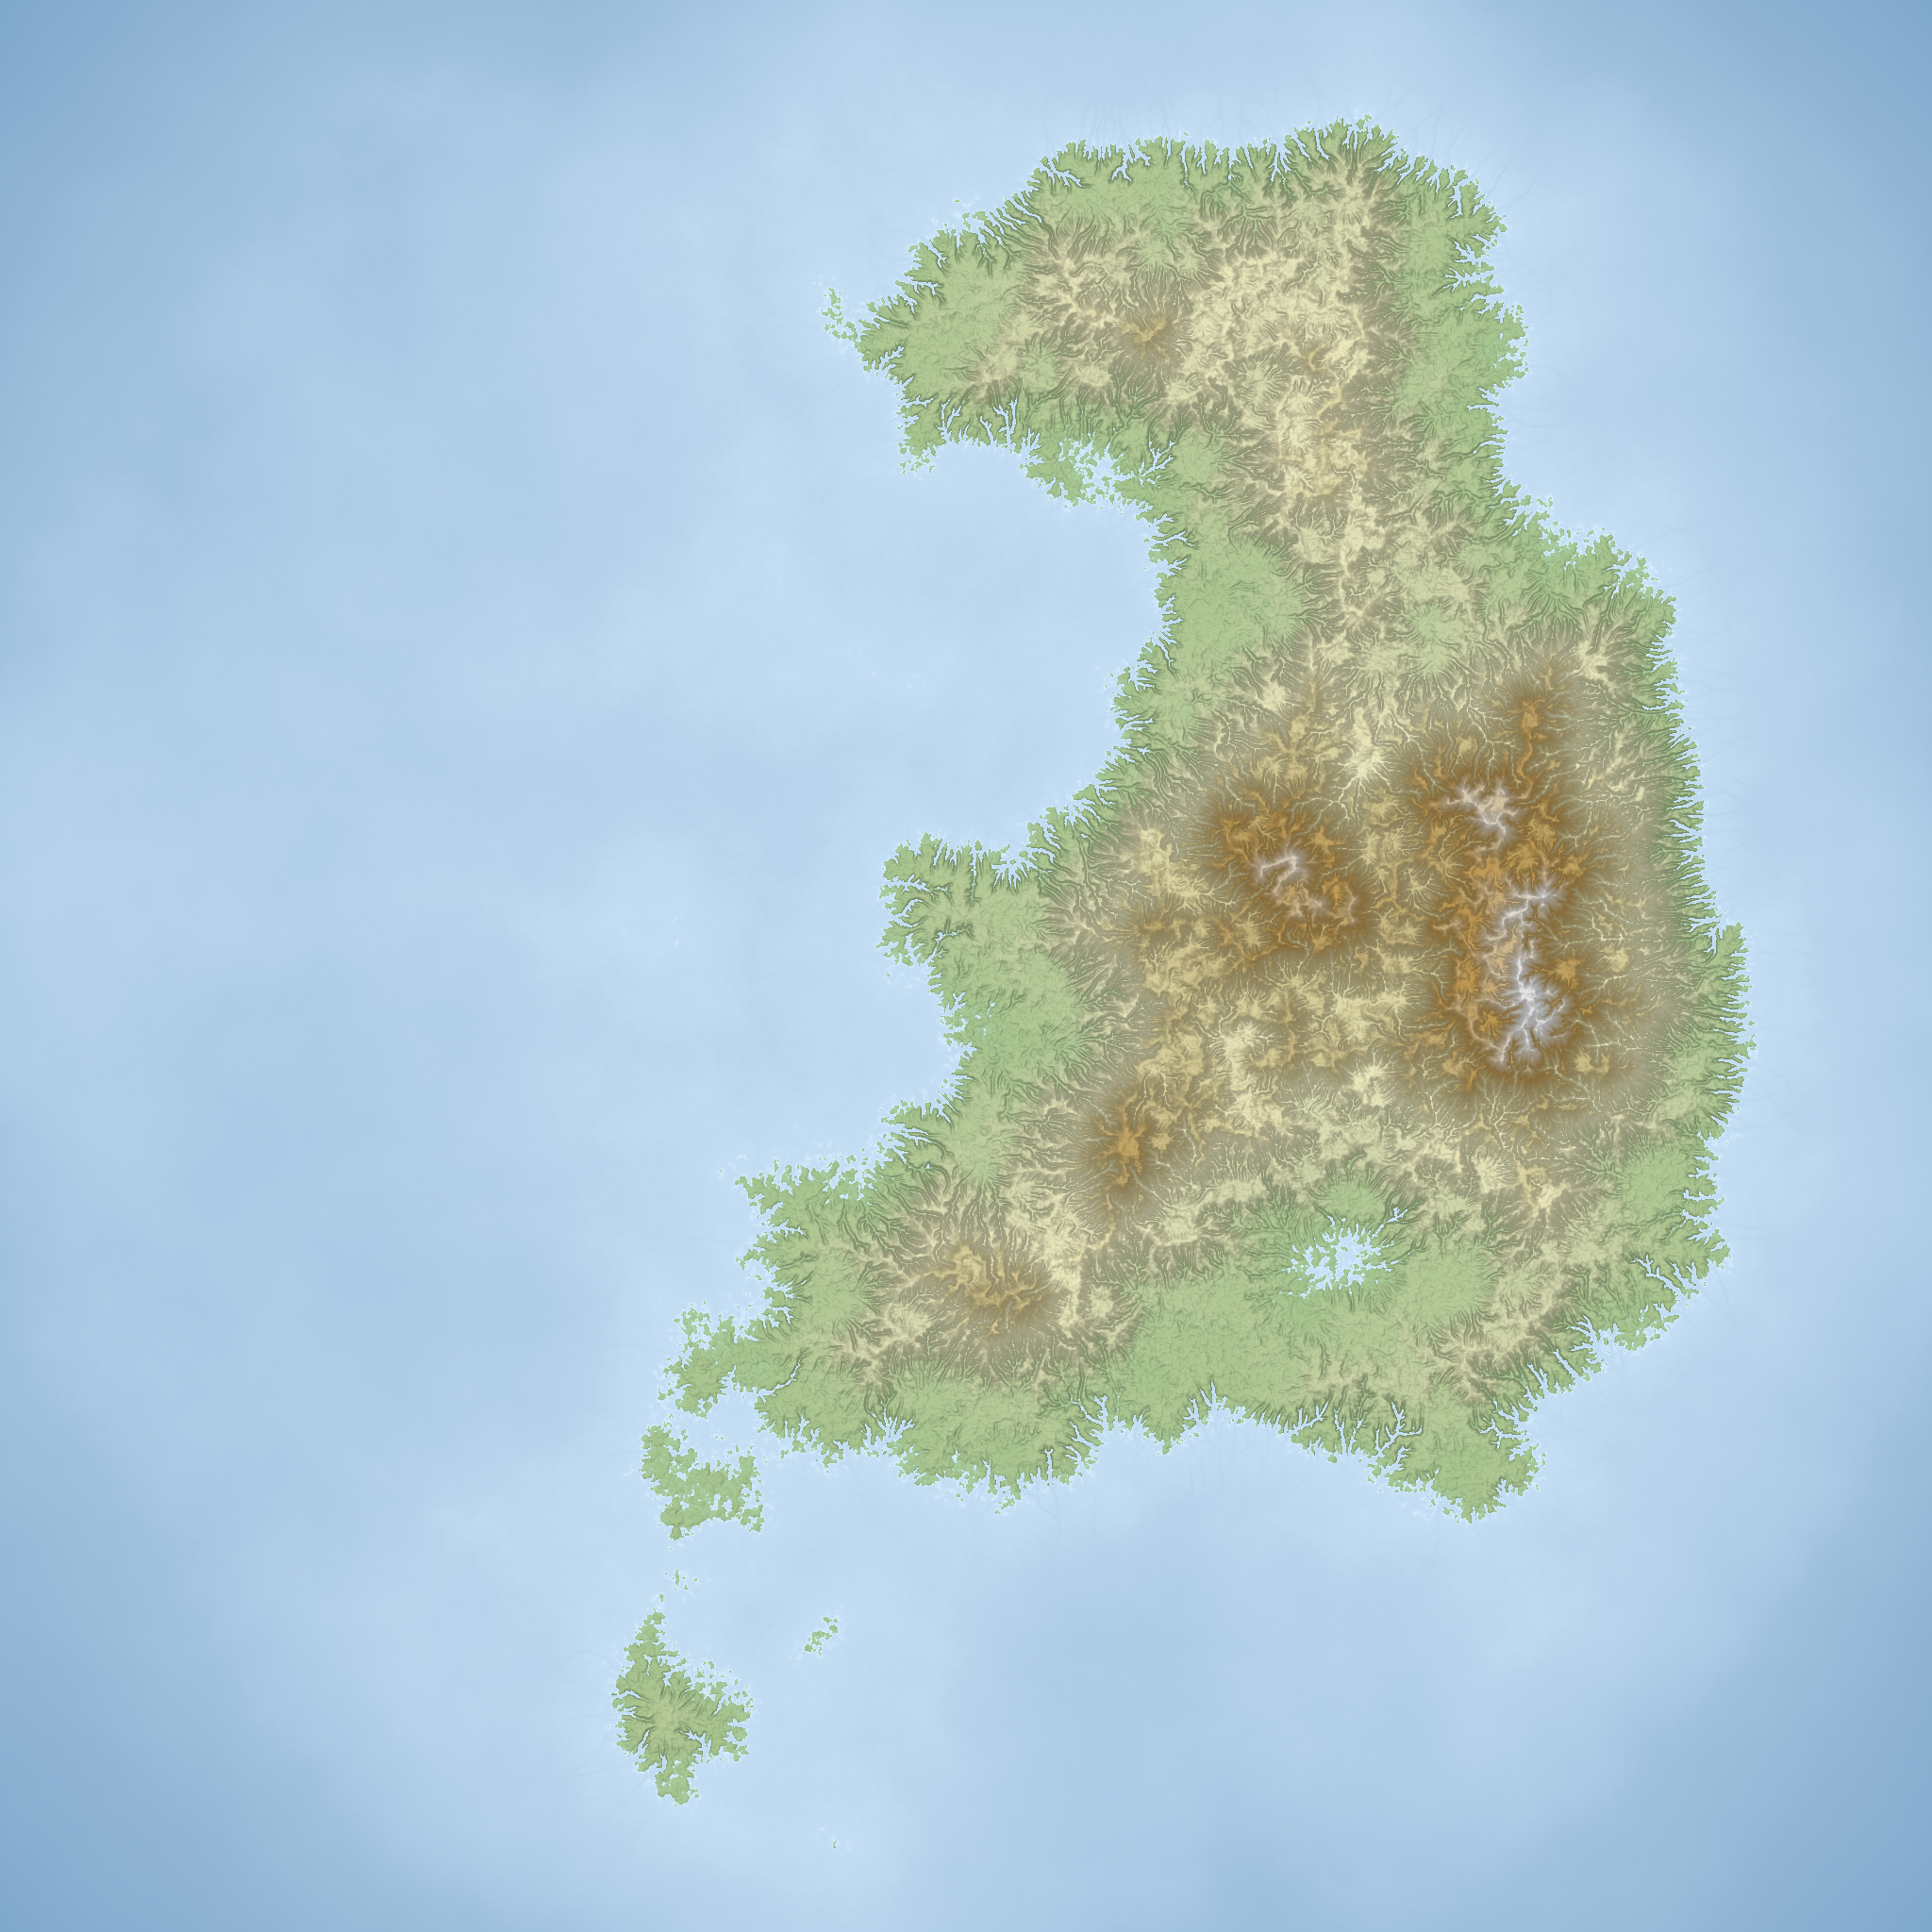
\includegraphics[width=0.9\textwidth]{data/86_rendered.png}}
\vskip 3ex

Úlohu si rozdelíme na menšíe časti a o každej z nich si niečo povieme.
Najprv si  vyrobíme 
výškovú mapu ({\em heightmap}): tabuľku \prg!double! s číslami z rozsahu\indexItem{Alg}{výšková mapa}
$0\ldots1$, kde $0$ znamená najmenšiu a $1$ najväčšiu výšku (obrázok A).
Z nej potom urobíme dva obrázky: jeden, ktorý bude určovať farbu získame tak,
že každému pixelu priradíme farbu z nejakého gradientu podľa jeho výšky (obrázok B)
a druhý, ktorý bude určovať tiene, vyrobíme  podľa sklonu terénu (obrázok C). Napokon
oba obrázky spojíme do výsledku (obrázok D).



\centerline{
  \begin{tikzpicture}[scale=5]
    \def\tmp#1{\includegraphics[width=3.8cm]{data/86_#1.png}}
    \node (A) at (0,0) {\tmp{heightmap}};
    \node (B) at (1,0) {\tmp{colored}};
    \node (D) at (2,0) {\tmp{rendered}};
    \node (C) at (1,-1) {\tmp{normal}};

    \foreach \a in {A,B,C,D}
    \node [above = of \a, yshift = -11mm] {(\a)};

    \draw[->] (A) -- (B);
    \draw[->] (B) -- (D);
    \draw[->] (A) to[out=270,in=180] (C);
    \draw[->] (C) to[out=0,in=270] (D);
  \end{tikzpicture}}

Začneme s prípravnou prácou: na zapisovanie finálneho výsledku môžeme použiť náš starý súbor
\hbox{\link{\rootpath/obrazok.h}{obrazok.h}.} Okrem toho budeme veľa robiť s tabuľkami,
kde budeme mať buď reálne čísla alebo farby, tak je dobré sa na to pripraviť.

\begin{uloha}
  Uprav triedu \vb{Tabulka} z kapitoly \ref{sect:cukor} tak, aby sa v nej 
  dali ukladať akékoľvek typy (pomocou šablóny).
\end{uloha}

Prvý pokus o náhodnú výškovú mapu môže vyzerať nejak takto\footnote{\indexItem{Prg}{inkrement \vb{i++} ako výraz}%
Tu idem použiť zápis, ktorý sme doteraz nemali a zaslúži si komentár. Ak mám napr. premennú
\prg!int i!, tak vieš, že \prg!i++! je príkaz, ktorý priráta k \prg!i! jednotku. Doteraz som ti
nepovedal, že \prg!i++! sa dá použiť aj ako výraz. Keby som mal napr. \prg!vector<int> a!,
tak \prg!int x = a[i++]! znamená \cmd{Do \prg!x! ulož hodnotu \prg!a[i]! a potom zvýš \prg!i! o jednotku}.
Je to teda to isté, ako keby som napísal \prg!x = a[i]; i = i+1;!.
Niekedy si možno zbadal aj zápis \prg!++i!, ktorý sám osebe robí to isté, t.j. pripočíta k \prg!i! jednotku,
ale urobí to na začiatku. Preto \prg!int y = a[++i]! je to isté ako \prg!i = i+1; y = a[i];!
}

\begin{lstlisting}
#include <algorithm>
#include <fstream>
#include <iostream>
#include <random>
#include <sstream>
#include <vector>

#include "obrazok.h"
#include "tabulka.h"

using namespace std;
mt19937 rnd(random_device{}());
uniform_real_distribution<> dis(0.0, 1.0);

void zapis(Tabulka<double>& T, const char* fname) {
  vector<unsigned char> data(T.m * T.n * 4);
  for (int i = 0; i < T.m; i++)
    for (int j = 0; j < T.n; j++) {
      int offs = 4 * ((T.n - j - 1) * T.n + i);
      for (int k = 0; k < 3; k++)
        // min a max sú z knižnice <algorithm> a vrátia menšie a väčšie z dvojice čísel
        data[offs++] = min(255 * max(T(i, j), 0.0), 255.0);
      data[offs++] = 255;
    }
  zapis_rgba_png(T.n, T.m, data.data(), fname);
}

int main(int argc, char** argv) {
  if (argc > 1) {
    unsigned long seed;
    stringstream ss(argv[1]);
    ss >> seed;
    rnd.seed(seed);
  }
  int n = 1024;
  Tabulka<double> T(n, n);
  for (int i = 0; i < n; i++)
    for (int j = 0; j < n; j++) T(i, j) = dis(rnd);

  zapis(T, "sum.png");
}
\end{lstlisting}


V tomto programe som si spravil pomocnú funkciu
\vb{zapis()}, ktorá zoberie tabuľku s výškovou mapou
a zapíše z nej obrázok do súboru tak, že nula je čierna a jednotka je biela. Pri zapisovaní 
obrázka potrebujem na jeden pixel štyri byty \vb{r,g,b,a}. Keďže chcem vyrobiť odtiene sivej,
hodnoty \vb{r,g,b} nastavím všetky rovnako, a to na hodnotu \vb{255 * T(i,j)}.

 
V hlavnom si vyrobím náhodný generátor a pozriem sa,  či nie je na príkazovom riadku parameter. Ak je, zoberiem ho ako seed. Ak budem 
chcieť zopakovať ten istý ostrov, stačí zadať rovnaký seed. Spustím program a výsledok je



\centerline{\begin{tikzpicture}[scale=0.8]

  \coordinate (A) at (-2mm,-2mm);
  \coordinate (B) at (4cm, 1cm);
  \draw[red] (A) -- (B);
  \filldraw[draw=red, fill=white] (A) circle (1mm) (B) circle (2.5cm);

  \node[anchor=north east] at (0,0) {
\includegraphics[width=6cm]{data/sum.png}};
  \node at (B) {
\includegraphics[width=2.6cm]{data/sum_big.png}};
  \draw[draw=red] (A) circle (1mm) (B) circle (2.5cm);
\end{tikzpicture}}


Ugh. Zväčšený roh vpravo ukazuje, prečo to nefunguje: keďže každý pixel je 
nezávislé náhodné číslo, nie je medzi nimi žiaden vzťah. Hodnoty medzi jednotlivými
pixelmi skáču tak, že výsledkom, keď sa naňho pozerám trochu z diaľky, je sivá plocha.
Potrebujem niečo, čo by síce bolo náhodné, ale zasa nie až tak úplne. Ukážem ti 
jednu z možností, ako náhodnosť regulovať. Volá sa podľa chlapíka, čo s tým prvý prišiel,\indexItem{Alg}{Perlin noise}
{\em Perlin noise}. S ním sa dajú generovať rôzne veľké náhodné vzory, ktorých kombináciou
vznikajú fraktálovité náhodné útvary.\\


% perlin 17
\centerline{\begin{tikzpicture}[scale=3.4]
  \foreach \i in {0,1} {
    \foreach \j in {0,1,2} {
      \pgfmathtruncatemacro{\tmp}{1+3*\i+\j}
      \node at (\j,-\i) {\includegraphics[width=31mm]{data/sample_perlin_\tmp.png}};
      }}

  \node[draw, single arrow, minimum height=12mm, minimum width=8mm,
  single arrow head extend=2mm, anchor=center] at (2.75,-0.5) {};

      \node at (3.5,-0.5) {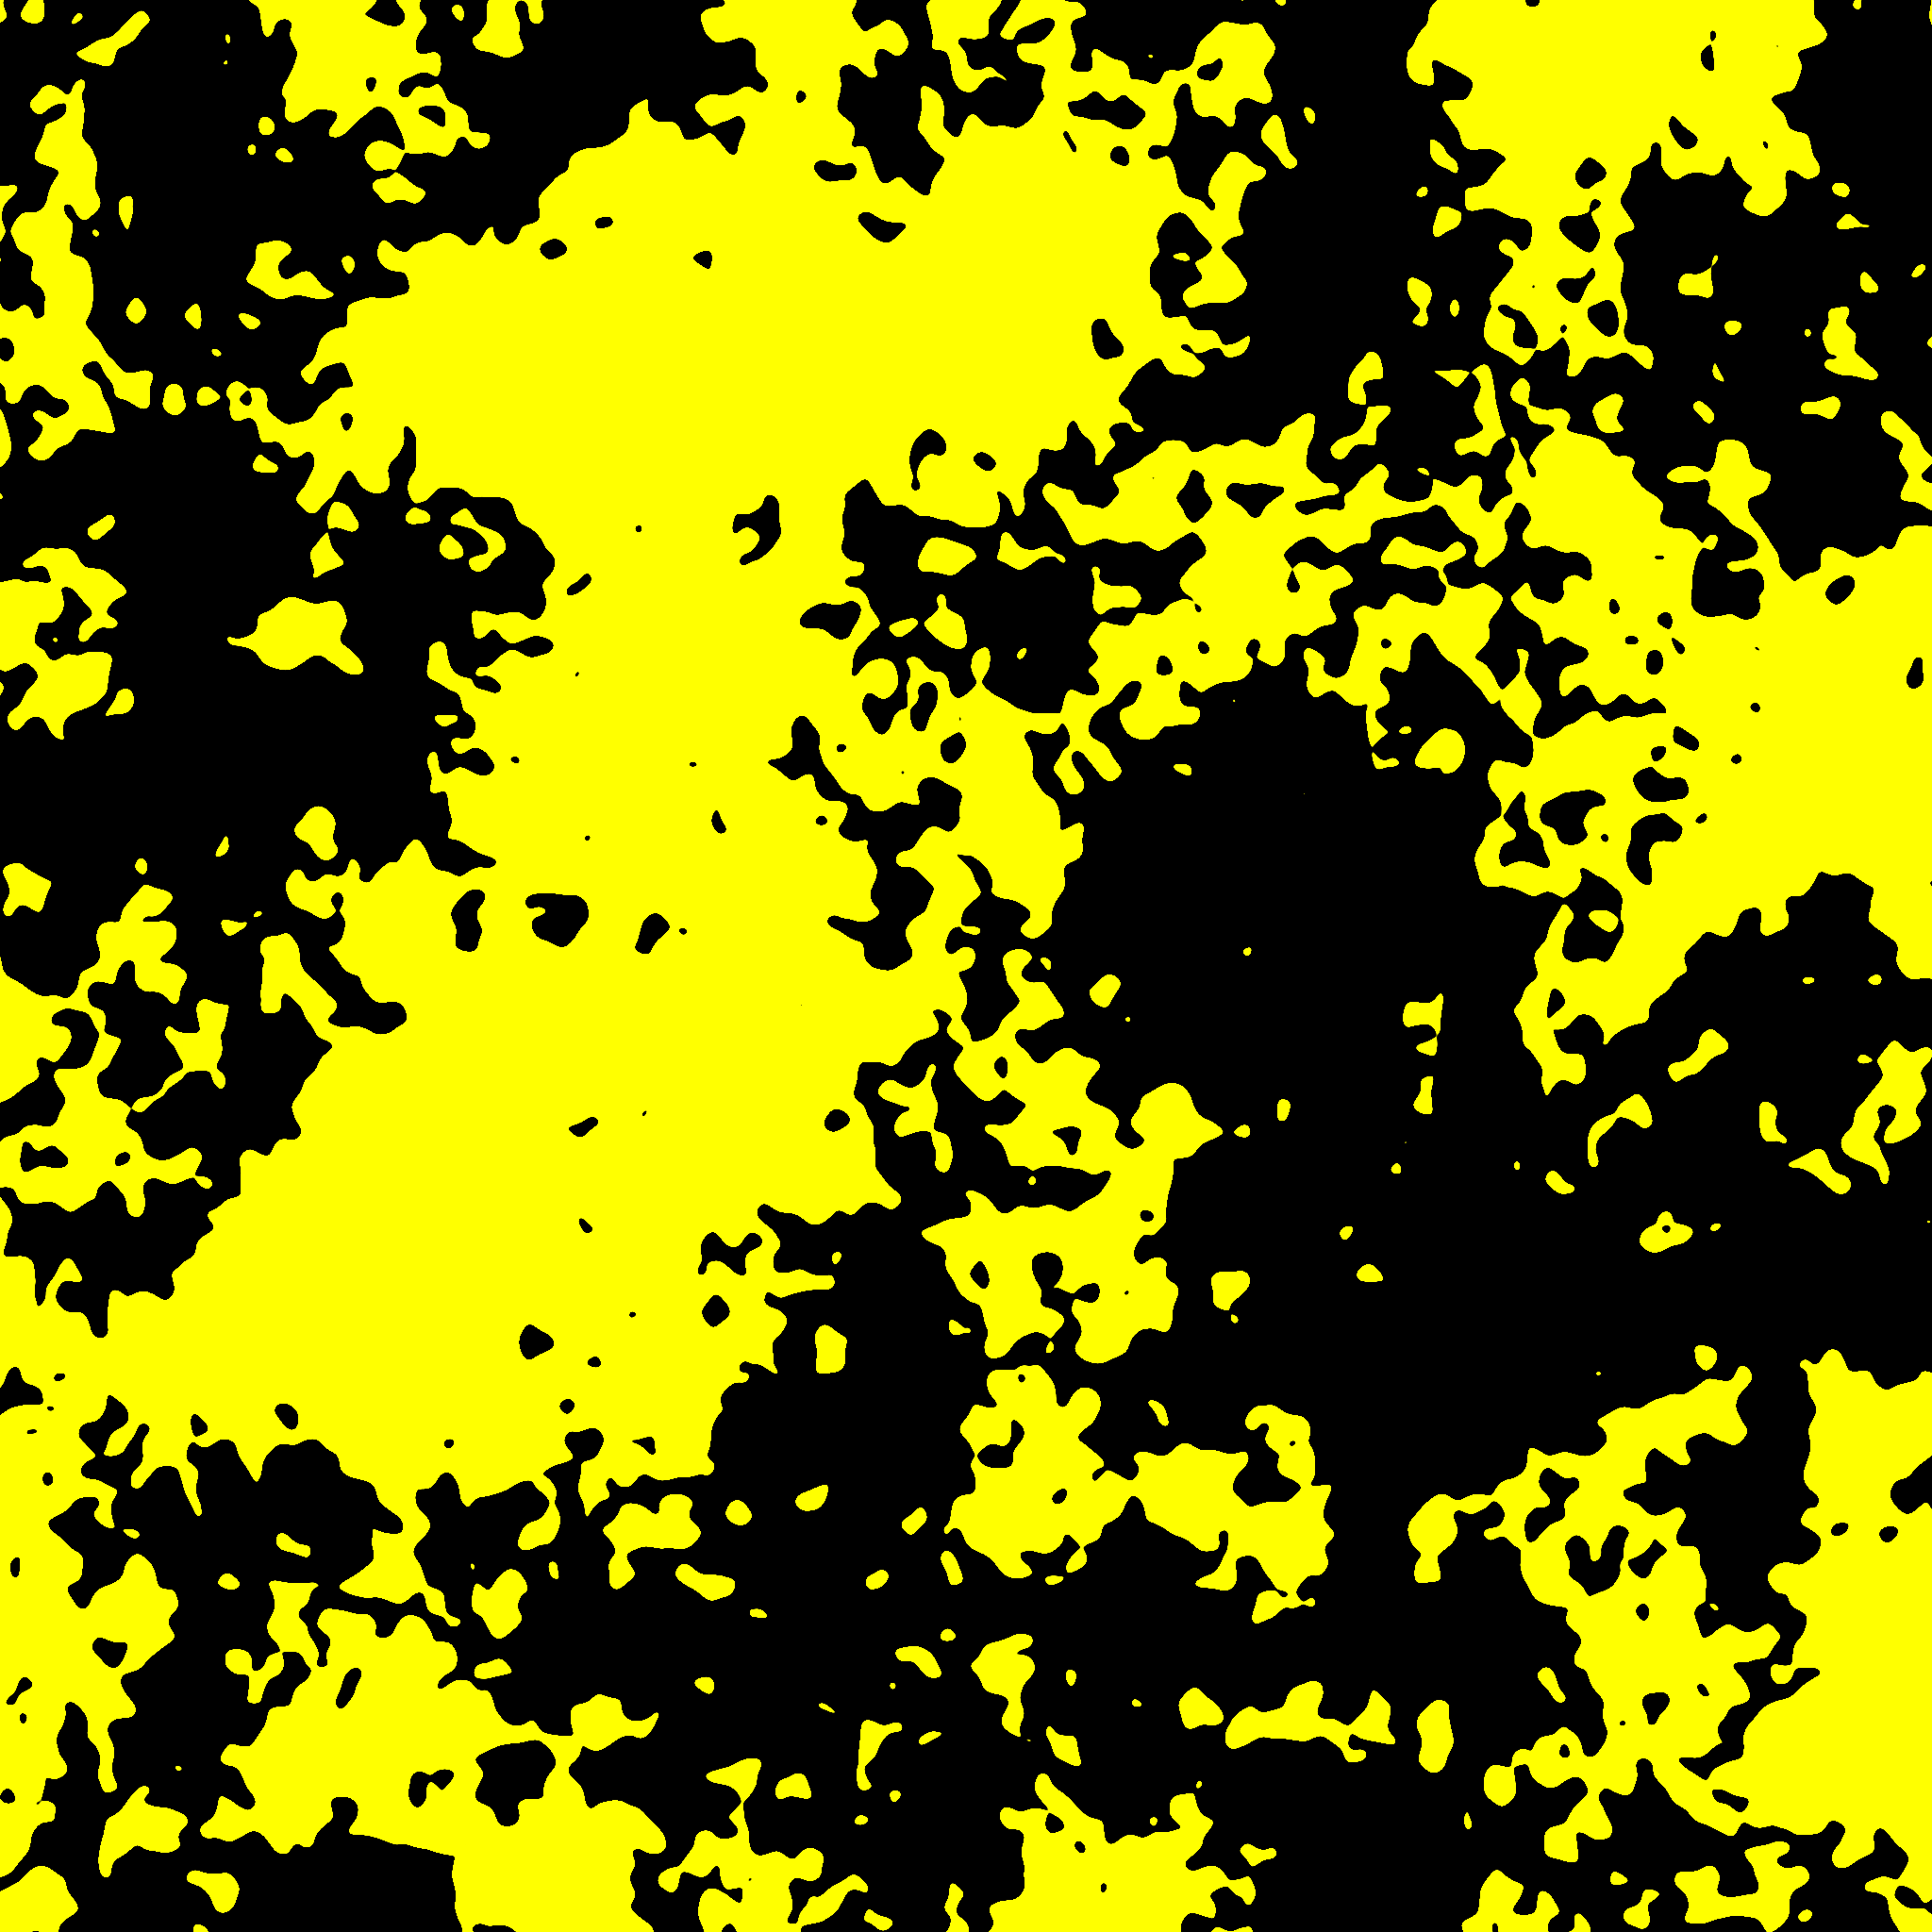
\includegraphics[width=3cm]{data/sample_perlin.png}};
      
\end{tikzpicture}}



Perlin noise najprv popíšeme matematicky a potom sa pozrieme na to, ako ho naprogramovať.
Zoberme si rovinu. Každému bodu chceme priradiť číslo tak, že čísla menšie ako $-1$ znamenajú
čiernu, čísla väčšie ako $1$ bielu a medzi nimi je spojitý prechod. Budeme tak dostávať 
obrázky ako ten nasledujúci ako vľavo. Keby sme chceli vzorku ako tá vpravo, môžeme každý bod zaokrúhliť: ak je
kladný, pixel bude žltý, ak je záporný, pixel bude čierny.\\


\centerline{
  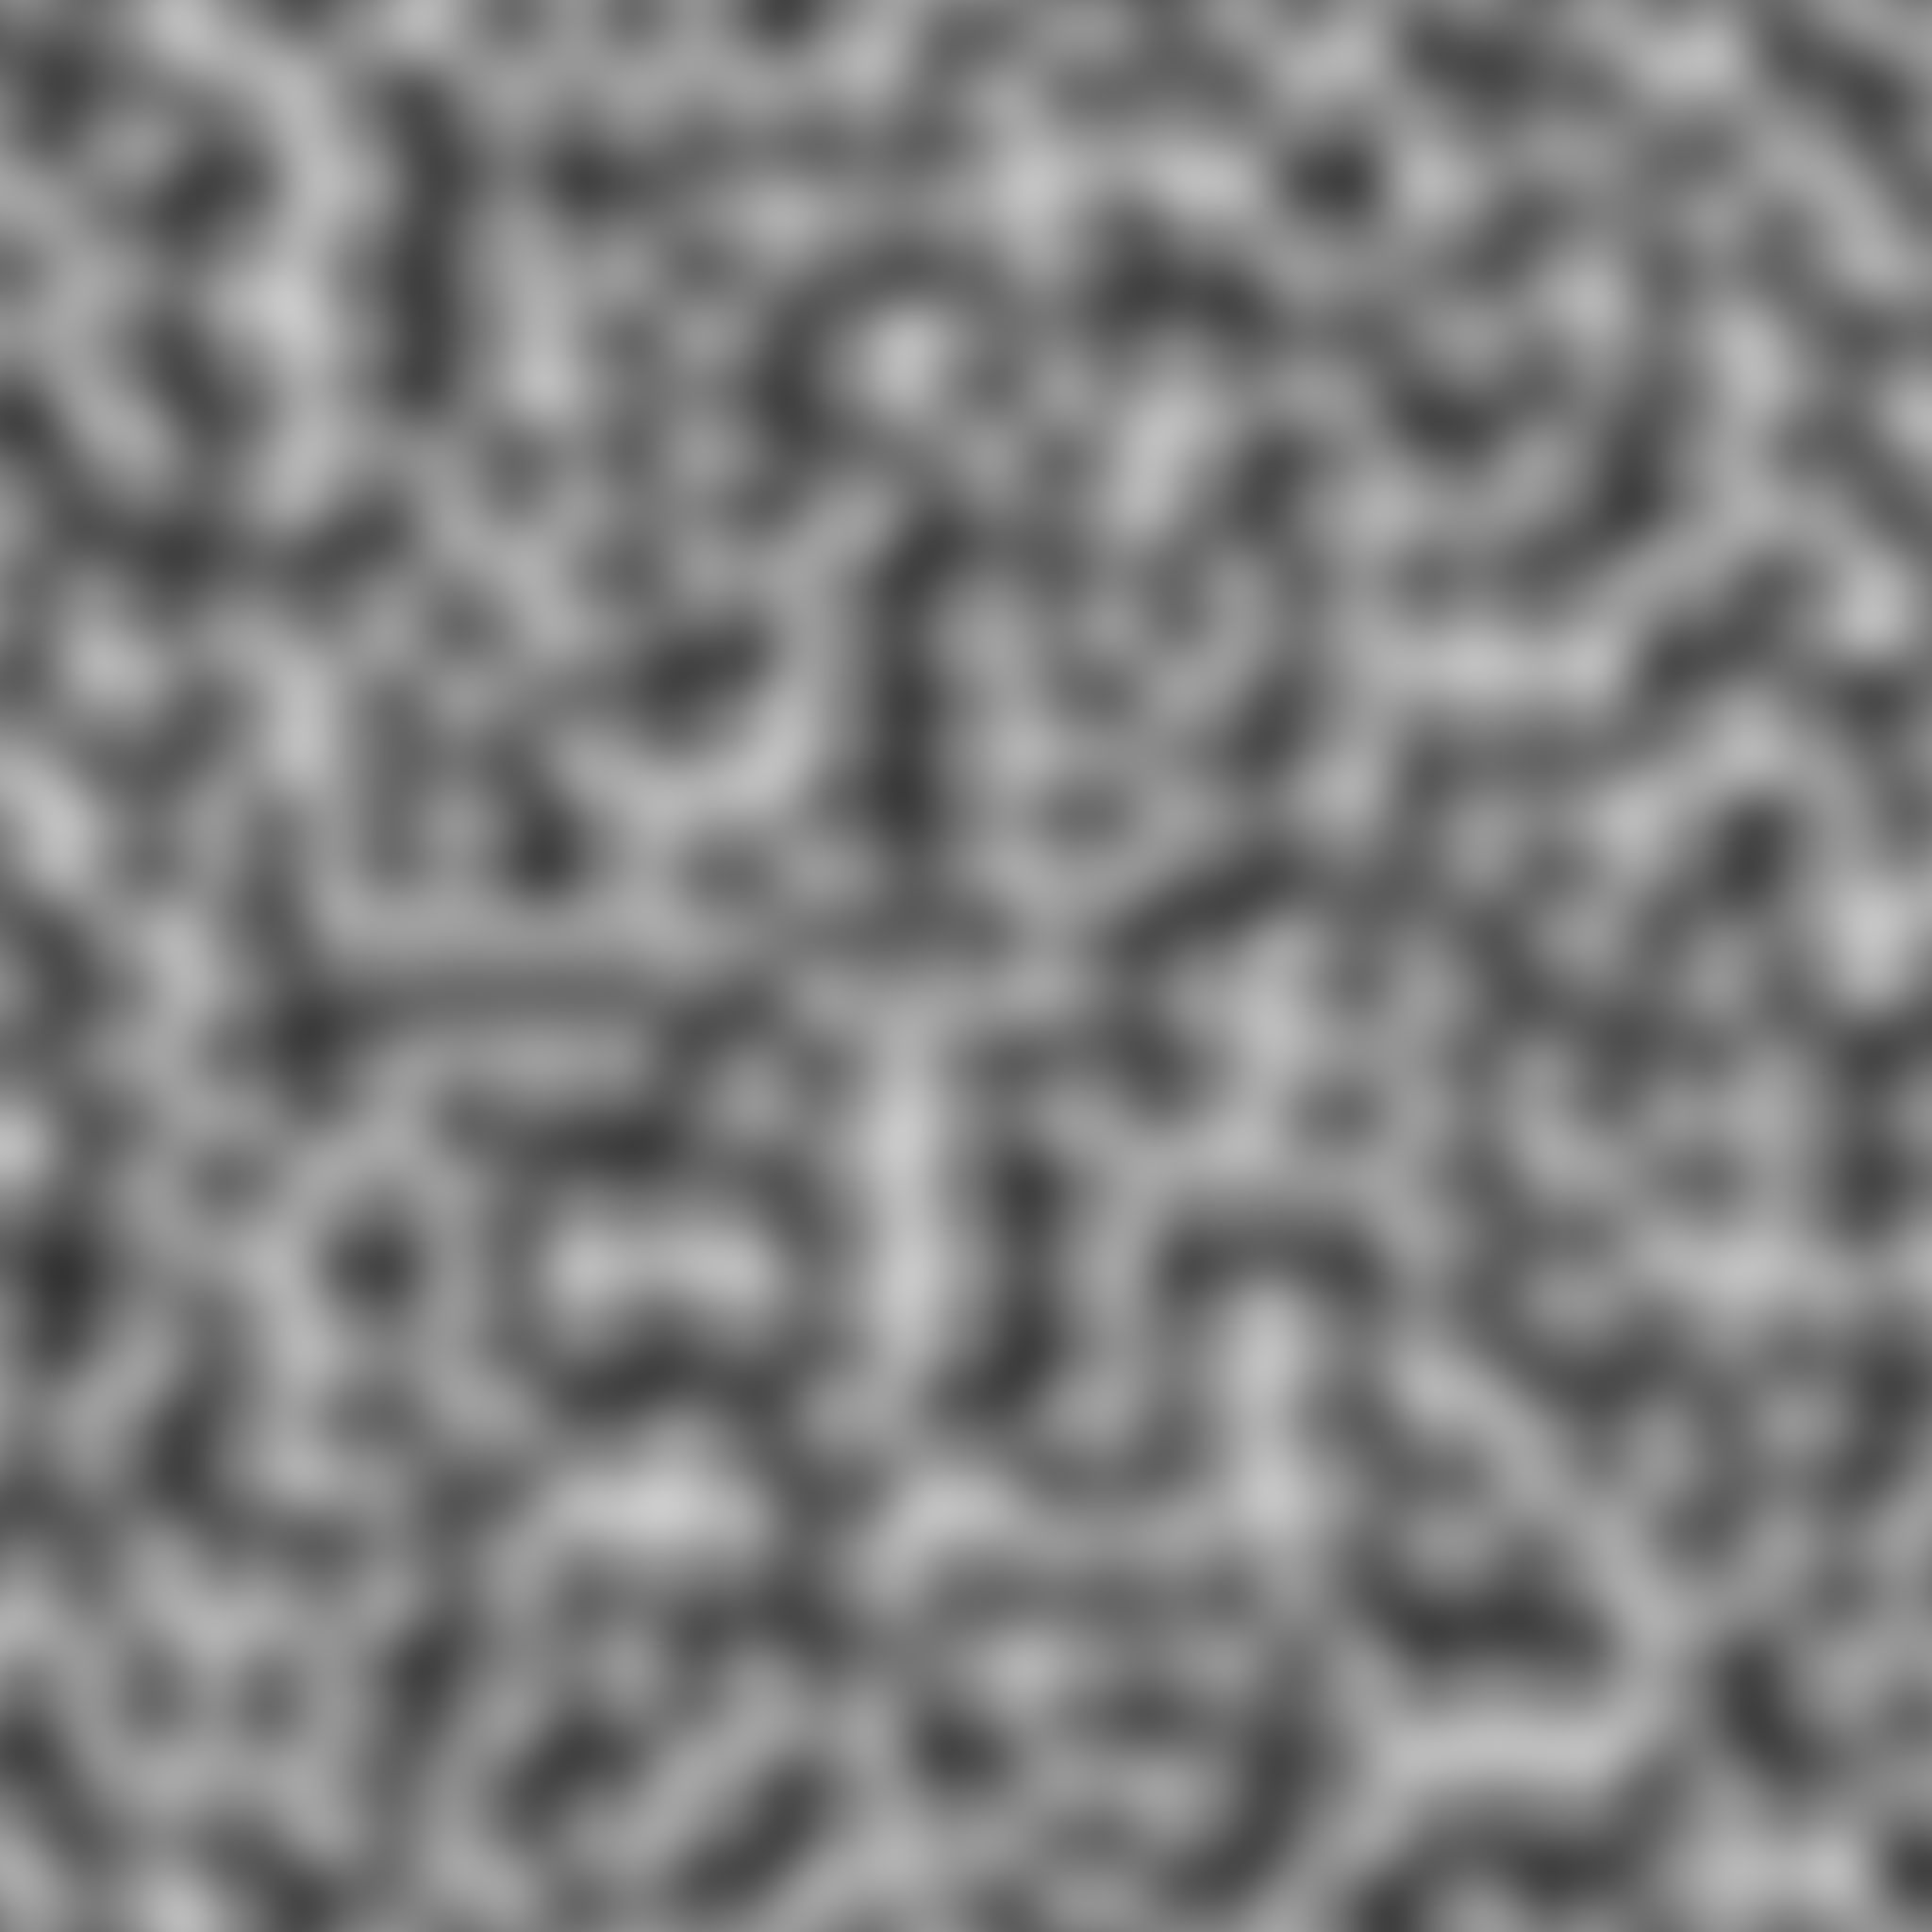
\includegraphics[width=0.4\textwidth]{data/perlin_single.png}
  \hskip 1cm
  
\includegraphics[width=0.4\textwidth]{data/perlin_single_crisp.png}
}


Základom pre vyrobenie obrázka vľavo je "natočený gradient". Zoberiem si nejaký bod $P$  a 
umiestnim doňho natočenú šípku. Tento gradient každému bodu v rovine 
priradí hodnotu podľa jeho pozície 
v smere šípky. Napr. ak mám šípku umiestnenú v bode $P=[-0.5,0.5]$, tak bodu $A$ sa
priradí číslo $0.7$ a bodu $B$ číslo $-0.4$.



\centerline{\begin{tikzpicture}[scale=1.5]
  \def\targetfill(#1)[#2]{% 
    \begin{scope}[shift={(#1)},rotate=#2]
    \shade[shading=axis,top color=white, bottom color = black, shading angle=40] 
    (0,0) circle (1);
  \end{scope}
  }
  \def\target(#1)[#2]{% 
    \begin{scope}[shift={(#1)},rotate=#2]
    \draw[red] (0,0) circle (1) (-1.5,0) -- (1.5,0);
  \draw[red,->] (0,-1.5) -- (0,1.5);
    \fill [red] (0,0) circle (0.35mm);
  \end{scope}
  }

  \def\point(#1)[#2]#3#4#5#6#7#8{
    \begin{scope}[shift={(#1)},rotate=#2]
      \coordinate (#5) at (0,#3);   
    \fill[#6] (#5) circle (0.35mm);
      \filldraw[#6, fill=#6, dashed] (#5) node[anchor=#7] {$#3$} -- ++(#4,0) 
      circle (0.35mm) node[anchor=south #8, black]{$#5$};
  \end{scope}
  }

  \coordinate (P) at (-0.5,0.5);
  \targetfill(P)[20]
  \draw[help lines, color=gray!30, dashed] (-2.9,-1.9) grid (2.9,2.9);
  \draw[->] (-3,0) -- (3,0) node[right] {$x$};
  \draw[->] (0,-2) -- (0,3) node[above] {$y$};
  \target(P)[20]
  \node[anchor=north east, red] at (P) {$P$};
  \point(P)[20]{0.7}{2.5}{A}{blue}{east}{west}
  \point(P)[20]{-0.4}{-1.5}{B}{green}{west}{east}

\end{tikzpicture}}

Výsledný obrázok získame tak, že si v rovine spravíme pravidelnú mriežku, 
v ktorej umiestnime náhodne otočené gradienty.
Každý bod roviny leží v nejakom štvorci mriežky a jeho výsledná farba sa určí kombináciou farieb zo
štyroch susedných gradientov.\\


\centerline{\begin{tikzpicture}[scale=3]
  \def\sza{0.2}
  \def\szb{0.36}
  \def\target(#1)[#2]{% 
    \begin{scope}[shift={(#1)},rotate=#2]
    \draw[red] (0,0) circle (\sza) (-\szb,0) -- (\szb,0);
  \draw[red,->] (0,-\szb) -- (0,\szb);
    \fill [red] (0,0) circle (0.15mm);
  \end{scope}
  }
  \node at (1,1) {
\includegraphics[width=6cm]{data/perlin_fixed.png}};
  \draw[help lines,color=gray!30, dashed] (0,0) grid (2,2);

  %perlin 12
  \foreach \x/\y/\a in 
  {0/0/80,0/1/140,0/2/140,1/0/280,1/1/190,1/2/30,2/0/170,2/1/90,2/2/130} {
    \target(\x,\y)[\a-90]
  }

  \coordinate (A) at (1.6,1.35);
  \filldraw[blue, dashed] (A) node[anchor=north] {$P$} circle (0.15mm) -- (1,1) (A) -- (1,2) (A) -- (2,1) (A) -- (2,2);
\end{tikzpicture}}


Kombináciu hodnôt urobíme podobne, ako sme robili interpoláciu farieb vo farebnom
gradiente v projekte o Mandelbrotovej množine,
až na to, že teraz potrebujeme interpolovať v dvoch rozmeroch (preto sa tomu hovorí {\em bilineárna interpolácia}).\indexItem{Alg}{bilineárna interpolácia}
Predstav si, že máme mriežku gradientov s krokom $d$ a chceme určiť farbu pre bod $P$ so súradnicami $[x,y]$.
Keď si všetky súradnice vydelím $d$čkom, mriežka bude mať krok $1$.
$P$ sa nachádza v mriežke medzi štyrmi bodmi $G_{00}$, $G_{10}$, $G_{01}$ a $G_{11}$.
Pripomeniem, že $\lfloor x\rfloor$ označuje celú časť z $x$, preto $G_{00}$ má súradnice
$\left\lfloor\frac{x}{d}\right\rfloor,\left\lfloor\frac{y}{d}\right\rfloor$ a ostatné 
4 body sú vždy o $1$ ďalej.


\centerline{\begin{tikzpicture}[scale=5.5]
  \def\ofs{0.2}
  \def\ofsi{0.35}
  \def\lclr{teal}
  \tikzstyle{link}=[dashed, thin, \lclr, shorten <= -0.6ex]
  \def\dot(#1)[#2]{\fill[#2] (#1) circle (0.007);}
  % pozicia, uhol, dlzka od-do, vyska, nazov suradnice
  \def\grr(#1)[#2](#3,#4)#5{
    \begin{scope}[shift={(#1)},rotate=#2]
      \draw[red] (-0.1,0) -- (0.1,0) (0,0) circle (0.05);
      \draw[->,red] (0,#3) -- (0,#4);
      \coordinate (#5) at ($(0,-100)!(P)!(0,100)$);
    \end{scope}
  }
  \draw[dashed] (0,0-\ofsi) node [below] {$\left\lfloor\frac{x}{d}\right\rfloor$} -- (0,0);
  \draw[dashed] (1,0-\ofsi) node [below] {$\left\lfloor\frac{x}{d}\right\rfloor+1$} -- (1,0);
  \draw[dashed] (1+\ofsi,0) node [right] {$\left\lfloor\frac{y}{d}\right\rfloor$} -- (1,0);
  \draw[dashed] (1+\ofsi,1) node [right] {$\left\lfloor\frac{y}{d}\right\rfloor+1$} -- (1,1);

  \draw (0-\ofs,0) -- (1+\ofs,0) (0-\ofs,1) -- (1+\ofs,1) (0,0-\ofs) -- (0,1+\ofs) (1,0-\ofs) -- (1,1+\ofs);
  \node[anchor = north east, inner sep=0.5cm] at (0,0) {$G_{00}$} ;
  \node[anchor = north west, inner sep=0.5cm] at (1,0) {$G_{10}$} ;
  \node[anchor = south east, inner sep=0.5cm] at (0,1) {$G_{01}$} ;
  \node[anchor = south west, inner sep=0.5cm] at (1,1) {$G_{11}$} ;
  

  \coordinate (P) at (0.43,0.6);
  
  \grr(0,0)[19](-0.15,0.5){v00} 
  \draw[link] (v00) node[anchor=north west] {$v_{00}$} -- (P);
  \dot(v00)[\lclr]
  
  \grr(1,0)[-30](-0.15,0.3){v10}
  \draw[link] (v10) node[anchor=north west] {$v_{10}$} -- (P);
  \dot(v10)[\lclr]

  \grr(0,1)[-62](-0.15,0.3){v01}
  \draw[link] (v01) node[anchor=south east] {$v_{01}$} -- (P);
  \dot(v01)[\lclr]

  \grr(1,1)[-130](-0.3,0.2){v11}
  \draw[link] (v11) node[anchor=south west] {$v_{11}$} -- (P);
  \dot(v11)[\lclr]


  \draw[blue,brace=1mm/](0,1.2)-- node[above=2.5ex]{$1$}(1,1.2);

  \coordinate (Px) at ($($(0,0)!(P)!(1,0)$) + (0,0-\ofs)$);
  \coordinate (Py) at ($($(0,0)!(P)!(0,1)$) + (0-\ofs,0)$);
 
  \draw[thin,lightgray]  (Px) -- ($(0,1)!(P)!(1,1)$)  (P)--(Py);
  \draw[blue,brace=1mm/mirror] (0,0-\ofs) -- node[below=2.5ex]{$r=\frac{x}{d}-\left\lfloor\frac{x}{d}\right\rfloor$} (Px);
   \draw[blue,brace=1mm/mirror] (Px) -- node[below=2.5ex]{$1-r$} (1,0-\ofs);

   \draw[blue,brace=1mm/] (0-\ofs,0) -- node[left=2.5ex]{$s=\frac{y}{d}-\left\lfloor\frac{y}{d}\right\rfloor$} (Py);
   \draw[blue,brace=1mm/] (Py) -- node[left=2.5ex]{$1-s$} (0-\ofs,1);

  \dot(P)[black]
  \node[anchor=west] at (P){$P\;\left[\frac{x}{d},\frac{y}{d}\right]$};
  \fill ($(0,0)!(P)!(1,0)$) node[anchor = north west]{$C$} circle (0.007)
   ($(0,1)!(P)!(1,1)$) node[anchor = south west]{$D$} circle (0.007);
\end{tikzpicture}}
%\pagebreak[1]


Predpokladajme, že sme už vyrátali hodnoty, ktoré prislúchajú bodu $P$ v
jednotlivých gradientoch a označili sme si ich
$v_{00}$, $v_{10}$, $v_{01}$ a $v_{11}$. Ako z nich skombinovať výslednú hodnotu v $P$? 
Desatinná časť po vydelení $x/d$ 
je $r=\frac{x}{d}-\left\lfloor\frac{x}{d}\right\rfloor$. Keby si bod $P$
posúval v štvorci zľava doprava, hodnota $r$ sa bude plynule meniť medzi $0$ a $1$.
Preto hodnotu v bode $C$ vieme interpolovať ako $v_C=v_{00}(1-r)+v_{10}r$. 
Podobne hodnotu v bode $D$ interpolujeme
$v_D=v_{01}(1-r)+v_{11}r$. 
Napokon urobíme rovnakým spôsobom interpoláciu medzi $v_C$ a $v_D$ v smere osi $y$, 
takže výsledok bude $v_C(1-s)+v_Ds$. 


Skoro dobré, ale  je tam stále drobný
problém: pretože interpolujeme lineárne iba v rámci jedného štvorca,
vznikajú nám nepekné zlomy ako vľavo, kým my potrebujeme hladký prechod ako vpravo\\


\centerline{
  
\includegraphics[width=0.4\textwidth]{data/perlinL_fixed.png}
  \hskip 1cm
  
\includegraphics[width=0.4\textwidth]{data/perlin_fixed.png}
}

\phantom{a}
\hfill
\begin{tikzpicture}
\begin{axis}[
  width=60mm, 
  height=6cm,
  domain=0:1,
  xmin=0,
  xmax=1,
  ymin=0,
  ymax=1,
  xlabel=$r$,
  /pgf/number format/.cd,
        1000 sep={}
]
  \addplot[no markers,red!50!white]{x};
  \addplot[no markers,green!50!white]{1-x};
\end{axis}
\end{tikzpicture}
  \hfill
\begin{tikzpicture}
\begin{axis}[
  width=60mm, 
  height=6cm,
  domain=0:1,
  xmin=0,
  xmax=1,
  ymin=0,
  ymax=1,
  xlabel=$6r^5-15r^4+10r^3$,
  /pgf/number format/.cd,
        1000 sep={}
]
  \addplot[no markers,red!50!white]{x * x * x * (10 + x * (6 * x - 15))};
  \addplot[no markers,green!50!white]{1-x * x * x * (10 + x * (6 * x - 15))};
\end{axis}
\end{tikzpicture}
\hfill
\phantom{a}


Hladký prechod sa dá dosiahnuť tak, že namiesto interpolácie s parametrami $r$ a $1-r$, ktoré
sú pri koncoch špicaté, budeme interpolovať s parametrami $f(r)$ a $1-f(r)$ pre nejakú
vhodnú funkciu $f$, ktorá je na koncoch hladká. Perlin odporúča zobrať 
$f(r)=6r^5-15r^4+10r^3$. Môžeme aj tak, prečo nie.

 
Teraz môžeme napísať takmer celý program na Perlin noise. 
Najprv si urobím pomocnú funkciu na lineárnu interpoláciu \vb{lerp}, ktorá sa
bude hodiť vo všeobecnejšej podobe


\begin{lstlisting}
template <typename T>
T lerp(const T& v0, const T& v1, double t) {
  return (1 - t) * v0 + t * v1;
}
\end{lstlisting}


Teraz vyrobím triedu \vb{Perlin},
ktorá bude mať dva parametre: \vb{n} veľkosť obrázka (pre jednoduchosť budem
robiť štvorcové obrázky rozmerov $n\times n$) a krok mriežky \vb{d}.
Zavolanie konštruktora vyrobí tabuľku \vb{H}, v ktorej bude výsledná výšková
mapa. Na natočené šípky budem mať triedu \vb{Vec} o ktorej si povieme viac o 
chvíľu, nateraz si ju predstav ako 


\begin{lstlisting}
struct Vec {
  double x, y;
};
\end{lstlisting}


Natočené šípky budú uložené v tabuľke $G$ rozmerov $m\times m$, kde 
$m=1+\left\lfloor\frac{n}{d}\right\rfloor$. V konštruktore
najprv vygenerujeme náhodné šípky tak, že zvolíme náhodný uhol \vb{theta} ($\theta$)
a šípka bude ukazovať do bodu so súradnicami $[\cos(\theta),\sin(\theta)]$
(o funkciách $\sin$ a $\cos$ pozri odbočku v kapitole~\ref{sect:editor}).
Potom už len vyrátam pre každý bod $P=[i,j]$ jeho farbu.
To znamená, že keď vyrobím premennú typu \vb{Perlin}, konštruktor vyrobí tabuľku \vb{H},
ku ktorej potom môžem pristupovať.


\begin{lstlisting}
struct Perlin {
  int n, d, m;  
  Tabulka<double> H;
  Tabulka<Vec> G;

  // konštruktor. 
  // všimni si zápis n\{\_n\} - niekedy je čitateľnejšie volať copy konštruktor 
  // pre int za dvojbodkou ako písať priradenie v tele konštruktora
  Perlin(int _n, int _d) : n{_n}, d{_d}, m{1 + n / d}, 
                           H(n, n), G(m, m) {
    for (int i = 0; i < m; i++)
      for (int j = 0; j < m; j++) {
        double theta = dis(rnd) * M_PI * 2.0;
        G(i, j) = {cos(theta), sin(theta)};
      }

    for (int i = 0; i < n; i++)
      for (int j = 0; j < n; j++) {
        // bod P so súradnicami [i,j]
        Vec p{ (double)i / (double)d,  (double)j / (double)d};

        // súradnice bodu G00
        int o[2] = {(int)p.x, (int)p.y}; 

        // hodnoty v00, v10, v01 a v11
        double v[4];

        ... // tu ich treba nejak vyrátať
        
        double r = fade(p.x - o[0]), s = fade(p.y - o[1]);
        double vc = lerp(v[0], v[1], r), vd = lerp(v[2], v[3], r);
        H(i, j) = lerp(vc, vd, s);
      }
  }

  // fade funkcia, ako ju odporúčal Perlin
  double fade(double t) {
    return t * t * t * (10 + t * (6 * t - 15));
  }
};
\end{lstlisting}


Ostáva doplniť posledná vec, a to ako vyrátať hodnoty $v_{00},\ldots,v_{11}$,
teda ako pre daný bod zrátať jeho výšku v nejakom natočenom gradiente. 
Predtým sa ale hodí

\section*{Matematické intermezzo: o bodoch a vektoroch}
\label{mat.body}

\indexItem{Mat}{bod, vektor}
Bod v rovine je vec, ktorá má dve súradnice, $x$ a $y$. Ak mám dva body, napr.
$A[x,y]$, $B[x',y']$, tak najkratšia cesta z bodu $A$ do bodu $B$ je úsečka, ktorá
sa v smere osi $x$ pohne o $x'-x$ a v smere osi $y$ o $y'-y$. Takýto úsečka
sa volá prenášač\indexItem{Mat}{vektor ako rozdiel bodov, sčitovanie vektorov} 
({\em vektor}) a dá sa zapísať dvoma číslami pre posun v $x$-ovom
a $y$-ovom smere, takže vyzerá
rovnako ako bod so súradnicami $[x'-x,y'-y]$. Je preto prirodzené
si to predstaviť tak, že ak odčítam od seba dva body, dostanem vektor.
Ak treba body a vektory rozlíšiť, nad vektory sa niekedy
zvykne písať šípka, napr. vektor $v$ je $\vec v = B-A$. 
Podobne keď k nejakému bodu $C$ prirátame vektor $\vec v$, 
dostaneme nový bod (ten, do ktorého nás
vektor prenesie).


\centerline{
\begin{tikzpicture}[scale=0.5]
  \tikzstyle{vecs}= [-{>[length=2ex,width=1.7ex]}]
  \def\dot(#1){\fill (#1)circle (1.8pt) }
  \draw[dotted,thin,gray] (-1,-1) grid (12,8);
  \coordinate (A) at (1,3);
  \coordinate (B) at (8,6);
  \draw[red,style=vecs](A) -- node[anchor = south east, inner sep=2mm]{$\vec v=B-A$}(B);
  \dot(A) node[anchor=north east]{$A$};
  \dot(B) node[anchor=south west]{$B$};
  \draw[thin, teal, dashed] 
  (A) -- ++(3,-2) coordinate (AA)
  (B) -- ++(3,-2) coordinate (BB);
  \draw[magenta, style = vecs] (AA) -- (BB);
  \dot(AA) node[anchor=north]{$C$};
  \dot(BB) node[anchor=north west]{$C+\vec v$};
  \draw[thin] (-1.5,0) -- (12.5,0) (0,-1.5) -- (0,8.5);
\end{tikzpicture}}

Vektory môžeme sčitovať prirodzeným spôsobom po zložkách (t.j. 
$[x,y]+[x',y']=[x+x',y+y']$), čo sa dá nakresliť ako skladanie šípok: na konci jednej
nakreslíme druhú:


\centerline{
\begin{tikzpicture}[scale=0.5]
  \tikzstyle{vecs}= [-{>[length=2ex,width=1.7ex]}]
  \def\dot(#1){\fill (#1)circle (1.8pt) }
  \draw[dotted,thin,gray] (-1,-1) grid (12,8);
  \coordinate (A) at (1,1);
  \coordinate (B) at ($(A)+(6,2)$);
  \coordinate (C) at ($(B)+(3,5)$);
  \dot(A); \dot(B); \dot(C);
  \draw[orange,style=vecs](A) -- node[anchor = north west, inner sep=1mm]{$\vec u=[6,2]$}(B);
  \draw[teal,style=vecs](B) -- node[anchor = north west, inner sep=1mm]
  {$\vec v=[3,5]$}(C);
  \draw[magenta,style=vecs](A) -- node[anchor = south east, inner sep=1mm]
  {$\vec u+\vec v=[9,7]$}(C);
  \draw[thin] (-1.5,0) -- (12.5,0) (0,-1.5) -- (0,8.5);
\end{tikzpicture}}


Rovnako dobre dáva zmysel, aby sme vektor vynásobili číslom: napr. ak 
$\vec v=[x,y]$, tak $4.2\cdot\vec v=[4.2x,4.2y]$ je
šípka v rovnakom smere ako $\vec v$, iba $4.2$-krát dlhšia. Podobne $-0.5\cdot\vec v$ je
šípka polovičnej dĺžky a v opačnom smere. 


Ak mám bod $A[x,y]$, tak si viem povedať, že to je vlastne vektor $A-[0,0]$, t.j.
šípka, ktorá ukazuje zo začiatku súradnicovej sústavy do $A$. Teraz je bod a vektor naozaj
to isté. Premysli si to: napr. $[9,7]-[3,5]=[6,2]$ môžem interpretovať tak, že mám bod
so súradnicami $[9,7]$ a bod so súradnicami $[3,5]$, tak vektor medzi nimi má súradnice $[6,2]$.
Ale rovnako môžem povedať, že ak mám vektor $[3,5]$, tak $-[3,5]$ je rovnako dlhý vektor v 
opačnom smere a $[9,7]+(-[3,5])$ je skladanie vektorov, ktorého výsledkom je vektor $[6,2]$.


Z Pytagorovej vety viem, že ak $\vec v$ je vektor so súradnicami $[x,y]$, tak jeho 
dĺžka je $\nrm{\vec v}=\sqrt{x^2+y^2}$. Ak obe súradnice vydelím dĺžkou, dostanem vektor
$\vec v'=\left[\frac{x}{\nrm{\vec v}},\frac{y}{\nrm{\vec v}}\right]$, ktorého dĺžka je 
$$\nrm{\vec v'}=\sqrt{\left(\frac{x}{\nrm{\vec v}}\right)^2+\left(\frac{y}{\nrm{\vec v}}\right)^2}
=\sqrt{\frac{x^2}{\nrm{\vec v}^2}+\frac{y^2}{\nrm{\vec v}^2}}
=\sqrt{\frac{1}{\nrm{\vec v}^2}(x^2+y^2)}=\sqrt{\frac{1}{\nrm{\vec v}^2}}\sqrt{x^2+y^2}=
\frac{1}{\nrm{\vec v}}\nrm{\vec v}=1
$$
Hovoríme, že $\vec v'$ je {\em normovaný} (resp. {\em normalizovaný}) vektor.\indexItem{Mat}{normalizovaný vektor}


\centerline{
\begin{tikzpicture}[scale=0.5]
  \tikzstyle{vecs}= [-{>[length=2ex,width=1.7ex]}]
  \def\dot(#1){\fill (#1)circle (1.8pt) }
  \draw[dotted,thin,gray] (-1,-1) grid (12,8);
  \coordinate (A) at (9,7);
  \draw[magenta, style=vecs] (0,0) -- (A) node[anchor=south west]{$\vec v = [x,y]$};
  \dot(0,0); \dot(A);
  \draw[thin] (-1.5,0) -- (12.5,0) (0,-1.5) -- (0,8.5);
  \draw[thin,gray](A) -- ($(0,0)!(A)!(10,0)$) coordinate(Ax);
  \draw[brace=1mm/] (A) -- node[anchor=west, xshift=2ex]{$y$} (Ax);
  \draw[thick, teal, style=vecs] (0,0) -- node[anchor=south east]{$1$}
  ($0.4*(A)$) coordinate(B) node[anchor=south east]{$\vec v'$};
  \dot(B);
  \draw[thin,gray](B) -- ($(0,0)!(B)!(10,0)$) coordinate(Bx);
  \draw[brace=1mm/] (B) -- node[anchor=west, xshift=2ex]{$\frac{y}{\nrm{\vec v}}$} (Bx);
\end{tikzpicture}}


Máme teda vektory, ktoré vieme sčitovať, odčitovať a násobiť reálnym číslom. Samozrejme, toto
všetko by rovnako dobre fungovalo v troch (a viacerých) rozmeroch. Môžeme ale nejak rozumne
vynásobiť dva vektory medzi sebou? 
Tu to už nie je také jednoznačné. Môžme vymyslieť rôzne 
operácie, ktoré nazveme súčin, a ktoré budú mať rôzne vlastnosti podľa toho, čo práve potrebujeme počítať. 
Jeden spôsob je uvedomiť si, že vektor v rovine so súradnicami $[x,y]$
je vlastne komplexné číslo $x+iy$, takže môžeme používať násobenie ako pri komplexných číslach.
Ukážem ti ešte dva iné spôsoby, ktoré sa nám budú hodiť, a to tzv.  {\em skalárny} a {\em vektorový} súčin.


\indexItem{Mat}{skalárny súčin}
Skalárny súčin je spôsob násobenia, ktorý je veľmi prirodzený napr. vo fyzike. Možno vieš, že fyzikálna
veličina {\em práca} je súčin sily a dráhy, t.j. ak pôsobí na teleso sila $1$N a posunie ho tým o $1$m,
vykoná pri tom prácu $1$J. Zvyčajne sa to zapisuje $W=Fd$.


\centerline{
  \begin{tikzpicture}[scale=1] 
  \draw[white] (0,0) -- (0,-0.8);
    \definecolor{acol}{rgb}{0.85,0.85,0.95}
    \node[xscale=-1,yscale=1,inner sep=0pt, anchor = south] (auto) at (2.7,0) {\textcolor{acol}{\usymH{1F69A}{1cm}}};    
    \node[xscale=-1,yscale=1,cyan!50!white,anchor=south, inner sep=0pt] (vlak) at (0,0) {\usymH{1F683}{1cm}};
    \draw[draw=acol, shorten <= 0.68cm, shorten >= 0.5cm, line width=0.6mm] 
    ($(vlak.center)+(0,-0.2)$) -- ($(auto.center)+(0,-0.2)$);
  %\node[xscale=-1,yscale=1,blue,anchor=south, inner sep=0pt] at (5,3) {\usymH{1F681}{1cm}};

    \draw (-1.5,0) -- (6,0);
  \foreach \x in {0,...,5}
  \draw (\x,-0.1) -- (\x,0.1);
    \fill[red] (vlak.center) circle (0.8mm);
    \draw[red,line width=0.6mm,->,>=latex] (vlak.center) -- node[above]{$F$} ++(3,0);
    \draw[cyan,line width = 0.6mm,->,>=latex] (0,-0.4) -- node[below]{$d$} (5,-0.4);
    \fill[cyan] (0,-0.4) circle (0.8mm);

\end{tikzpicture}
}


Tu sa ale potichu predpokladá, že sila aj dráha sú čísla, a preto ich môžem násobiť. Lenže v skutočnosti sila aj dráha sú
vektory a môžu pôsobiť rôznym smerom


\centerline{
  \begin{tikzpicture}[scale=1] 
  \draw[white] (0,0) -- (0,-0.8);
    \definecolor{acol}{rgb}{0.85,0.85,0.95}
   % \node[xscale=-1,yscale=1,inner sep=0pt, anchor = south] (auto) at (2.7,0) {\textcolor{acol}{\usymH{1F69A}{1cm}}};    
    \node[xscale=-1,yscale=1,blue,anchor=south, inner sep=0pt] (heli) at (4,2.5) {\textcolor{acol}{\usymH{1F681}{1cm}}};
    \node[xscale=-1,yscale=1,cyan!50!white,anchor=south, inner sep=0pt] (vlak) at (0,0) {\usymH{1F683}{1cm}};
    \draw[draw=acol, shorten <= 0.8cm, shorten >= 0.3cm, line width=0.6mm] 
    (vlak.center) -- ($(heli.center)+(0,-0.3)$) coordinate (lano);

    \draw (-1.5,0) -- (6,0);
  \foreach \x in {0,...,5}
  \draw (\x,-0.1) -- (\x,0.1);
    \draw[cyan,line width = 0.6mm,->,>=latex] (vlak.center) -- node[below]{$\vec d$} ++(5,0) coordinate (endD);
    \draw[red,line width=0.6mm,->,>=latex] (vlak.center) -- node[above]{$\vec F$} ($(vlak.center)!0.8!(lano)$) 
    coordinate(endF);
    \draw[thin, gray, dashed] (endF) -- ($(vlak.center)!(endF)!(endD)$) coordinate(fin);
    \draw[thin, ->, >=latex ] (vlak.center) -- (fin);
    \def\len{0.95cm}
    \draw[thin] ($(vlak.center)!\len!(endD)$) arc(0:28:\len);
    \fill[red] (vlak.center) circle (0.8mm);
\end{tikzpicture}
}


V tomto prípade sa časť sily, ktorou pôsobí vrtuľník, vyplytvá na nadľahčovanie vagóna a prácu robí 
iba tá časť, ktorá je rovnobežná s dráhou, takže na vyrátanie práce násobím
dĺžku vektora $\vec d$ a priemetu $\vec F$ (čierna šípka na obrázku). 
Aby sa zachoval rovnaký zápis, chcel by som násobiť vektory tak,
aby som mohol napísať $W=\vec F\cdot\vec d$. Ako sa také násobenie dá urobiť? Výsledkom násobenia dvoch vektorov
musí byť číslo, ktoré vznikne vynásobením dĺžky jedného a priemetu druhého:


\centerline{
\begin{tikzpicture}[scale=0.5]
  \tikzstyle{vecs}= [-{>[length=2ex,width=1.7ex]}]
  \def\dot(#1){\fill (#1)circle (1.8pt) }
  \draw[dotted,thin,gray] (-1,-1) grid (12,7);
  %\draw[thin] (-1.5,0) -- (12.5,0) (0,-1.5) -- (0,8.5);
  \def\degi{20}
  \def\degii{40}
  \coordinate (A) at (\degi:12cm);
  \coordinate (B) at ($(0,0)!7.5cm!\degii:(A)$);
  \draw[magenta, vecs] (0,0) -- node[pos=0.8, below]{$\vec u$}(A);
  \draw[teal, vecs] (0,0) -- node[anchor = east]{$\vec v$}(B);
  \coordinate (Bx) at ($ (0,0)!(B)!(A) $);
  \draw[thin,gray] (B) -- (Bx)
     ($(0,0)!1.5cm!(A)$) arc (\degi:\degi+\degii:1.5cm)
     ($(Bx)!4mm!(0,0)$) arc (180+\degi:90+\degi:4mm)
     ;
  \node at ($(0,0)!1cm!0.5*\degii:(A)$) {$\alpha$};
  \draw[teal, brace=1mm/mirror](0,0) -- node[rotate=\degi,below=2mm]{$\nrm{\vec v}\cos(\alpha)$} (Bx);
  \dot(0,0);\dot(A);\dot(B);
\end{tikzpicture}}


Výsledok by teda mal byť $\vec u\cdot\vec v=\nrm{\vec u}\cdot\nrm{\vec v}\cdot\cos(\alpha)$, kde $\alpha$ označuje
uhol, ktorý tie dva vektory zvierajú. Teraz idem trochu počítať a na záver mi vyjde, že takýto skalárny
súčin sa dá veľmi jednoducho vyrátať. Tak poďme na to. Zoberme si vektory $\vec u$, $\vec v$ ako na predchádzajúcom obrázku
a označme si $a=\nrm{\vec u}$, $b=\nrm{\vec v}$, $p=b\cos(\alpha)$. Situácia teda vyzerá takto:


\centerline{
\begin{tikzpicture}[scale=0.5]
  \tikzstyle{vecs}= [-{>[length=2ex,width=1.7ex]}]
  \def\dot(#1){\fill (#1)circle (1.8pt) }
  \draw[dotted,thin,gray] (-1,-1) grid (12,7);
  %\draw[thin] (-1.5,0) -- (12.5,0) (0,-1.5) -- (0,8.5);
  \def\degi{20}
  \def\degii{48}
  \coordinate (A) at (\degi:12cm);
  \coordinate (B) at ($(0,0)!6cm!\degii:(A)$);
  \draw[magenta] (0,0) -- node[pos=0.8, below]{$a$}(A);
  \draw[teal] (0,0) -- node[anchor = east]{$b$}(B);
  \coordinate (Bx) at ($ (0,0)!(B)!(A) $);
  \draw[thin,gray] (B) -- node[anchor=west] {$c$} (Bx)
     ($(0,0)!1.5cm!(A)$) arc (\degi:\degi+\degii:1.5cm)
     ($(Bx)!4mm!(0,0)$) arc (180+\degi:90+\degi:4mm)
     (B) -- node [anchor=south west]{$d$} (A)
     ;
  \node at ($(0,0)!1cm!0.5*\degii:(A)$) {$\alpha$};
  \draw[teal, brace=1mm/mirror](0,0) -- node[rotate=\degi,below=2ex]{$p$} (Bx);
  \dot(0,0);\dot(A);\dot(B);
  \node[anchor=north east] at (0,0) {$[0,0]$};
  \node[anchor=west] at (A) {$[u_x,u_y]$};
  \node[anchor=south] at (B) {$[v_x,v_y]$};
\end{tikzpicture}}


\tikzexternaldisable
\def\mathnode(#1)#2{\tikz[remember picture,baseline=(#1.base)]\node[draw=none, inner sep=0pt, outer sep=0pt](#1){$#2$};}

Potrebujeme vyrátať skalárny súčin $\nrm{\vec u}\cdot\nrm{\vec v}\cdot\cos(\alpha)$, t.j. v našom označení
$ap$. Všimneme si dva pravouhlé trojuholníky: jeden so stranami $b$, $p$, $c$ a druhý so stranami $d$, $a-p$, $c$.
Z Pytagorovej vety dostaneme pre prvý z nich $p^2=b^2-c^2$ a pre druhý $c^2=d^2-(a-p)^2$. Keď to dáme dokopy,
dostaneme $p^2=b^2-d^2+(a-p)^2$. Teraz roznásobíme $(a-p)^2=(a-p)\cdot(a-p)=a^2-2ap+p^2$, takže máme
$$p^2=b^2-d^2+a^2-2ap+p^2$$
a teda
$$2ap=\mathnode(b){b^2}+\mathnode(a){a^2}\mathnode(d){-d^2}$$
Teraz si dosadím $b^2=\nrm{\vec v}^2=v_x^2+v_y^2$, $a^2=\nrm{\vec u}^2=u_x^2+u_y^2$  a 
$d^2=(u_x-v_x)^2+(u_y-v_y)^2$ a dostanem
$$2ap=\mathnode(bb){v_x^2+v_y^2}+\mathnode(aa){u_x^2+u_y^2}\mathnode(dd){-(u_x-v_x)^2-(u_y-v_y)^2}$$

\begin{tikzpicture}[remember picture, overlay, draw opacity=0.6] 
  \def\spoj[#1]#2#3{
  \node[fit=(#2),draw=#1, rounded rectangle,inner xsep=0] (tmp1) {};
  \node[fit=(#3),draw=#1, rounded rectangle,inner xsep=0] (tmp2) {};
  \draw[#1] (tmp1)--(tmp2);
 }
  \spoj[teal]b{bb}
  \spoj[magenta]a{aa}
  \spoj[blue]d{dd}
\end{tikzpicture}
\tikzexternalenable



Keď si roznásobím $(u_x-v_x)^2=u_x^2-2u_xv_x+v_x^2$ a $(u_y-v_y)^2=u_y^2-2u_yv_y+v_y^2$ a dosadím,
dostanem
$$ap=u_xu_y+v_xv_y$$


Takže si to zhrňme: ak mám dva vektory $\vec u=[u_x,u_y]$ a $\vec v=[v_x,v_y]$, tak\\
\phantomsection\label{page:dotproduct-angle}

\centerline{\fbox{
  $\vec u\cdot\vec v=\nrm{\vec u}\cdot\nrm{\vec v}\cdot\cos(\alpha) = u_xu_y + v_xv_y$}}


Toto sa často hodí, lebo $u_xu_y + v_xv_y$ sa dá zrátať ľahko a rýchlo a ak sú $\vec u$ a $\vec v$ normované,
čiže ich dĺžka je $1$, tak priamo vyrátam kosínus uhla medzi nimi. 
Keď si nakreslím, ako závisí kosínus od veľkosti uhla, dostanem známy obrázok


\centerline{
\begin{tikzpicture}
\begin{axis}[
  width=0.6*\textwidth, 
  height=5cm,
  axis x line=middle,
  axis y line=left,
  axis line style={-},
  xtick={0,90,...,360},  
  xlabel=$\alpha$,
  xticklabel={\pgfmathtruncatemacro{\tmp}{\tick}$\tmp^\circ$},
  ylabel=$\cos(\alpha)$,
  scaled x ticks=false,
  scaled y ticks=false,
  domain=0:360,
  xmin=0,
  xmax=360,
  ymin=-1.1,
  ymax=1.1,
  /pgf/number format/.cd,
        1000 sep={}
]
  \addplot[dashed,very thin,gray!50!white]{1};
  \addplot[dashed,very thin,gray!50!white]{-1};
  \addplot[samples=1000,no markers,red!50!white]{cos(x)};
\end{axis}
\end{tikzpicture}}


Špeciálne, viem rýchlo zistiť, či sú dva vektory
kolmé: stačí overiť, či ich skalárny súčin je rovný nule. A, samozrejme, síce sme to všetko rátali v rovine, 
ale pre trojrozmerné vektory by to fungovalo úplne rovnako.


\indexItem{Mat}{vektorový súčin}
Iný spôsob súčinu, ktorý sa ale dá použiť iba pre trojrozmerné vektory, je tzv. {\em vektorový súčin}. 
Ak máš rovinu v 3D priestore  (napr. list papiera na stole) a v nej nakreslené hocijaké úsečky, tak 
existuje jeden smer, ktorý je kolmý na každú z nich:


\centerline{
  %\tikzset{external/force remake}
  \pgfmathsetseed{42} 
  \def\pravitko{
    %credit: https://tex.stackexchange.com/questions/289026/is-there-a-triangular-protractor-shape-built-in-to-tikz
    \begin{scope}[font=\scriptsize\sffamily]
      \filldraw[fill=white] (0:8) -- (180:8) -- (270:8) -- cycle;
\foreach \i in {225,315} \draw (\i:1) -- (\i:3) (\i:4.8) -- (\i:5.4);
\draw (-5.2,-0.5) -- ++(-1.6,0) (5.2,-0.5) -- ++(1.6,0);
\foreach \i [evaluate={\x=sqrt(4.25^2-\i^2);}] in {0.5,1,...,3.5}
  \draw [double=black, white, line width=0.125cm] (-\x,-\i) -- (\x,-\i);
\fill [white] (-2,-.25) rectangle (-2.75,-4)
  (2,-.25) rectangle (2.75,-4) (-.25,-.25) rectangle(.25,-4);
\foreach \i in {1,...,3} \draw (0,-\i+.25) -- ++(0,-0.5);
\foreach \i [evaluate={\x=sqrt(4.5^2-(\i/10)^2); \n=int(\i/10);
    \j=int(mod(\i,5)==0); \k=int(mod(\i,10));}] in {3,...,35}
  \draw (-2.5,-\i/10) -- ++(.1+\j/10,0) \ifnum\k=0 node [right]{\n}\fi
    (2.5,-\i/10) -- ++(-.1-\j/10,0) \ifnum\k=0 node [left]{\n}\fi;
\foreach \i [evaluate={\x=8*sin(45)/sin(\i>90 ? \i-45 : 135-\i); \n=int(180-\i);
    \t=(mod(\i,5)==0)/10+.1; \k=int(mod(\i,10));}] in {1,...,179}
  \draw (180+\i:\x) -- \ifnum\k=0 (180+\i:4.5)
      node [align=center, fill=white,rotate=\i-90, below=\t cm]
      {\ifnum\n=90 \n\else\n \\ \i\fi} \else ++(\i:\t)
     \ifnum\i>4 \ifnum\i<176 (180+\i:4.5) -- ++(180+\i:\t) \fi \fi \fi;
\foreach \i [evaluate={\n=int(abs(\i/10));
  \t=(mod(\i,5)==0)/10+.1; \k=int(mod(\i,10));}] in {-70,-69,...,70}
  \draw (\i/10, 0) -- ++(0,-\t,0) \ifnum\k=0 node [inner ysep=1,below]{\n}\fi;
\end{scope}
  }
  \begin{tikzpicture}[x={(1cm,0)},y={(45:0.4cm)},z={(0,1cm)},scale=3.5]
    \begin{scope}[plane x={(1.2,0,0)}, plane y={(0,1.2,0)},canvas is plane]
      \draw[teal,fill=teal!2!white](0,0) rectangle (2,2);
      \clip(0,0) rectangle (2,2);
      \foreach \i in {0,...,15} { 
        \pgfmathsetmacro{\x}{2*random()}
        \pgfmathsetmacro{\y}{2*random()}
        \pgfmathsetmacro{\a}{365*random()}
        \pgfmathsetmacro{\d}{0.3*(1+random())}
        \draw[gray] (\x,\y) -- ++(\a:\d);
      }
    \end{scope}
    \begin{scope}[
        shift={(1,2.5)},
        plane x={(-0.707,-0.707,1)}, 
        plane y={(0.707,0.707,1)},
        canvas is plane, 
        scale=0.05,
        every node/.style={scale=0.05},
      ]
      \pravitko
      \coordinate (A) at (270:8);
      \coordinate (v) at ($(0:8)-(A)$);
      \draw[red,thick,->] (A) -- ++($1.3*(v)$);
    \end{scope}
\end{tikzpicture}}



Takýto smer sa volá {\em normála} danej roviny. \indexItem{Mat}{normála roviny}
Pri vektorovom súčine, ako už názov napovedá, budeme počítať
vektor. Predpokladajme, že máme dva (3D) vektory $\vec u=[u_x,u_y,u_z]$ a $\vec v=[v_x,v_y,v_z]$.
Ich vynásobením dostaneme výsledný (3D) vektor $\vec w = \vec u\times\vec v$. Budeme chcieť, aby výsledok
$\vec w$ mal smer normály na rovinu, v ktorej ležia $\vec u$ a $\vec v$.
Okrem smeru si treba povedať, či má výsledok ísť "hore", alebo "dolu". Budeme chcieť,
aby platilo {\em pravidlo pravej ruky}: ak prstami pravej ruky ukážeš na $\vec u$ a 
vystretým palcom na $\vec v$, tak vrch dlane\footnote{
Všimni si, že tu 
na rozdiel od násobenia čísel alebo skalárneho súčinu záleží na poradí: 
$\vec u\times\vec v = - (\vec v\times\vec u)$.}
smeruje v smere $\vec u\times\vec v$:



\def\drawaxes{
    \draw[->,red, shorten >= 1ex] (0,0,0) -- (1,0,0) node{$x$};
    \draw[->,blue, shorten >= 1ex] (0,0,0) -- (0,1,0) node{$y$};
    \draw[->,teal, shorten >= 1ex] (0,0,0) -- (0,0,1) node {$z$};
  }


  \def\dTop[#1]{
    \begin{scope}[shift={(-0.38,0.5)}, xscale=-0.035, yscale=0.035, rotate=180]
      \draw[#1] svg {
    M -222.4252,370.46736 c 0,0 78.09933,-22.17038 100.9605,-16.10231 22.861172,6.06807 29.734046,20.38226 29.734046,20.38226 M 440.64946,-194.35246 c 0,0 5.6006,28.67018 15.53887,33.55993 9.93827,4.88975 29.07667,2.75792 40.11647,-4.71822 11.0398,-7.47613 2.6584,-42.39384 2.6584,-42.39384 M 331.92538,-344.75552 c 0,0 10.5773,31.36565 19.05613,36.27131 8.47883,4.90566 38.66552,1.57788 46.6844,-2.75128 8.01889,-4.32916 13.04957,-28.99798 13.04957,-28.99798 m -168.21416,-65.26014 c 6.17756,6.7793 0.79099,44.79739 13.80913,54.33948 13.01813,9.54209 43.85403,8.04415 55.38827,-0.24686 11.53425,-8.29101 8.84669,-30.10841 13.34782,-48.71803 m -161.1727,37.82961 c 2.11459,15.88406 -7.10301,42.73975 5.15248,51.50172 12.25549,8.76197 44.27784,7.69222 54.09212,2.11102 9.81428,-5.5812 8.32915,-32.96517 14.59136,-47.47943 m 7.79262,386.89534 C 224.20737,-87.455926 247.01408,-223.02691 237.7098,-356.1561 M 340.65006,35.549554 c 20.6969,-129.446566 -3.35315,-251.423144 -9.22294,-391.272874 M 440.83115,40.143094 c 9.16226,-83.966041 5.25395,-154.765284 -1.47033,-253.679384 m 84.6313,985.31679 c 5.14063,-161.34618 -18.47246,-233.61793 12.2561,-384.90278 30.72856,-151.28486 0.10128,-377.4470077 -17.32204,-528.91029 -11.09678,-93.47475 -59.76563,-105.90303 -79.56536,-71.50372 -5.18752,-32.53045 -12.34357,-70.65561 -26.89081,-123.11994 -14.54724,-52.46434 -65.6584,-49.84388 -81.04289,-19.0671 -2.32956,-15.4439 -2.78331,-21.82281 -6.38058,-44.39569 -5.76212,-36.15738 -60.84633,-32.7517 -72.95168,-19.1531 -11.16337,12.54043 -17.71816,44.91631 -14.38506,63.11602 -12.90154,-32.51953 -42.8587,-39.58443 -67.60334,-14.51906 -24.74464,25.06537 -32.79482,122.07217 -38.52995,237.91753 -5.73513,115.845355 -11.6547,247.60428 -1.89143,315.06657 9.29954,64.25795 -61.626269,88.29667 -132.0797675,67.0549 C -82.962511,225.0726 -146.264,240.93281 -199.57633,273.69211 c -53.31233,32.7593 -40.85268,118.55039 9.88565,107.09053 25.36916,-5.72993 121.342795,-14.01058 213.797195,8.97984 92.454405,22.99042 77.496795,73.09061 141.457855,104.09156 59.4688,28.82362 63.58928,198.90556 65.32075,281.53398
  };
    \end{scope}
  }


  \def\dBot[#1]{
    \begin{scope}[shift={(-1.1,0.35)}, xscale=-0.035, yscale=0.035, rotate=180]
      \draw[#1] svg {
    M 776.84581,381.52487 C 778.0352,266.09775 895.49019,170.55962 1056.6595,218.77989 m 360.6665,151.68747 c 0,0 -78.0994,-22.17038 -100.9605,-16.10231 -22.8612,6.06807 -29.7341,20.38226 -29.7341,20.38226 M 949.39833,30.73924 c 21.2951,-118.195166 -1.5116,-253.76615 7.7926,-386.89534 M 854.25073,35.549554 c -20.6969,-129.446566 3.3531,-251.423144 9.2229,-391.272874 m -109.404,395.866414 c -9.1623,-83.966041 -5.254,-154.765284 1.4703,-253.679384 m -84.6313,985.31679 c -5.1406,-161.34618 18.4725,-233.61793 -12.2561,-384.90278 -30.7285,-151.28486 -0.1013,-377.4470077 17.3221,-528.91029 11.0967,-93.47475 59.7656,-105.90303 79.5653,-71.50372 5.1875,-32.53045 12.3436,-70.65561 26.8908,-123.11994 14.5473,-52.46434 65.6584,-49.84388 81.0429,-19.0671 2.3296,-15.4439 2.7833,-21.82281 6.3806,-44.39569 5.7621,-36.15738 60.8463,-32.7517 72.9517,-19.1531 11.1633,12.54043 17.7181,44.91631 14.385,63.11602 12.9016,-32.51953 42.85867,-39.58443 67.60337,-14.51906 24.7446,25.06537 32.7948,122.07217 38.5299,237.91753 5.7352,115.845355 11.6548,247.60428 1.8915,315.06657 -9.2996,64.25795 61.6263,88.29667 132.0798,67.0549 80.5678,-24.29124 143.8693,-8.43103 197.1816,24.32827 53.3123,32.7593 40.8527,118.55039 -9.8857,107.09053 -25.3691,-5.72993 -121.3427,-14.01058 -213.7971,8.97984 -92.4545,22.99042 -77.4968,73.09061 -141.4579,104.09156 -59.46877,28.82362 -63.58927,198.90556 -65.32077,281.53398
  };
    \end{scope}
}


\centerline{
%\tikzset{external/force remake}
\tdplotsetmaincoords{50}{210}
\begin{tikzpicture}[tdplot_main_coords,scale=3.5]
\begin{scope}[plane x={(0,-0.9,0)}, plane y={(0.9,0,0)},canvas is plane]
  \dTop[gray,fill=orange!10!white]
    \draw[->,red] (0,0) -- (0,1.1) node[anchor=east]{$\vec u$};
    \draw[->,blue] (0,0) -- (160:1) node[anchor=north east]{$\vec v$};
\end{scope}
    \draw[->,teal] (0,0,0) -- (0,0,0.8) node[above] {$ \vec u\times\vec v$};
\end{tikzpicture}
\hfill
\tdplotsetmaincoords{50}{210}
\begin{tikzpicture}[tdplot_main_coords,scale=3.5]
    \draw[->,magenta] (0,0,0) -- (0,0,-0.8) node[below] {$ \vec v\times\vec u$};
\begin{scope}[plane x={(0,-0.9,0)}, plane y={(0.9,0,0)},canvas is plane]
  \begin{scope}[rotate=80]
  \dBot[gray,fill=orange!10!white]
  \end{scope}
    \draw[->,red] (0,0) -- (0,1.1) node[anchor=east]{$\vec u$};
    \draw[->,blue] (0,0) -- (160:1) node[anchor=north east]{$\vec v$};
\end{scope}
\end{tikzpicture}

}


Pri označovaní osí sa zvyčajne používa tzv. pravoruký systém, takže ak si nazvem
$\vec x=[1,0,0]$, $\vec y=[0,1,0]$ a $\vec z=[0,0,1]$, tak chcem, aby
$\vec x\times\vec y = \vec z$ a $\vec y\times\vec x=-\vec z$.
Ak mám vektor $\vec u=[u_x,u_y,u_z]$, tak 
$\vec u = u_x\vec x+ u_y\vec y+u_z\vec z$ a podobne
$\vec v = [v_x,v_y,v_z] = v_x\vec x+ v_y\vec y+v_z\vec z$.
V $z$-ovej súradnici výsledku by preto mohlo byť $u_xv_y$ s kladným znamienkom 
a $u_yv_x$ so záporným. A rovnako v ostatných dimenziách. To nás nabáda k definícii\\


\centerline{\fbox{$
[u_x,u_y,u_z]\times[v_x,v_y,v_z]=[
  u_yv_z-u_zv_y, 
  u_zv_x-u_xv_z, 
  u_xv_y-u_yv_x
]
$}}


Teraz si vieme ľahko overiť, že takto vymyslený súčin je to, čo chceme, totiž že
$\vec u\times\vec v$ je kolmý na $\vec u$ aj $\vec v$. Stačí použiť, čo sme si ukázali
pred chvíľou, totiž že kolmé vektory majú skalárny súčin $0$.
Preto rátajme


\tikzexternaldisable
\def\nd#1#2{\tikz[remember picture,baseline=(#1.base)]\node[draw=none, inner sep=0pt, outer sep=0pt](#1){\ensuremath{#2}};}

\begin{align*}
  (\vec u\times\vec v)\cdot \vec u &= 
[ u_yv_z-u_zv_y,u_zv_x-u_xv_z, u_xv_y-u_yv_x]\cdot[u_x,u_y,u_z] =\\
  &= (u_yv_z-u_zv_y)u_x+(u_zv_x-u_xv_z)u_y+( u_xv_y-u_yv_x)u_z = \\
  &= \nd{a}{u_yv_zu_x} - \nd{b}{u_zv_yu_x} + \nd{c}{u_zv_xu_y} 
    - \nd{d}{u_xv_zu_y} + \nd{e}{u_xv_yu_z} - \nd{f}{u_yv_xu_z} = \\
  &=0
\end{align*}
\begin{tikzpicture}[remember picture, overlay, draw opacity=0.6]
  \def\bx[#1]#2{
  \node[fit=(#2),draw=#1, rounded rectangle,inner xsep=0] {};
  }
  \bx[teal]{a}
  \bx[teal]{d}
  
  \bx[blue]{b}
  \bx[blue]{e}

  \bx[magenta]{c}
  \bx[magenta]{f}
\end{tikzpicture}
\tikzexternalenable

Preto $\vec u\times\vec v$ je kolmý na $\vec u$ a rovnako by sme vyrátali,
že je kolmý na $\vec v$.


Vektorový súčin sa dá, okrem počítania normály v 3D, použiť napr. na počítanie orientácie vektorov v 2D.
Zoberme vektory $\vec u=[u_x,u_y]$ a $\vec v=[v_x,v_y]$. Doplním ich do troch rozmerov, ako keby ležali v rovine
so $z=0$: $[u_x,u_y,0]$ a $[v_x,v_y,0]$ a vyrátam vektorový súčin $[0,0,u_xv_y-u_yv_x]$. Ak je $z$-ová súradnica
kladná, uhol, ktorý vektorý zvierajú je orientovaný proti smeru hodinových ručičiek, ak je záporná, tak v smere.


Posledná užitočná vlastnosť vektorového súčinu, ktorú tu spomeniem, je jeho veľkosť. Podobnými počtami, ako 
pri skalárnom súčine\footnote{iba trochu dlhšími, preto ich tu nebudem písať} sa dá vidieť, že\\


\centerline{\fbox{$\nrm{\vec u\times\vec v}=\nrm{\vec u}\cdot\nrm{\vec v}\cdot\sin(\alpha)$}}


Ak mám v priestore dva vektory, ktoré nie sú rovnobežné, definujú mi rovnobežník takto:


\centerline{
\begin{tikzpicture}[scale=0.3]
  \tikzstyle{vecs}= [-{>[length=2ex,width=1.7ex]}]
  \def\dot(#1){\fill (#1)circle (1.8pt) }
  \def\degi{5}
  \def\degii{65}
  \coordinate (A) at (\degi:12cm);
  \coordinate (B) at ($(0,0)!7cm!\degii:(A)$);
  \coordinate (Bx) at ($ (0,0)!(B)!(A) $);
  \coordinate (C) at ($ (A)+(B) $);
  
 \fill[yellow!10!white] (0,0) -- (A) -- (C) -- (B) -- cycle;
  \draw[dotted,thin,gray] (-1,-1) grid (15,9);
  \node at ($(0,0)!0.8cm!0.5*\degii:(A)$) {$\alpha$};
  \draw ($(0,0)!1.5cm!(A)$) arc (\degi:\degi+\degii:1.5cm);
  \draw[thick,teal,vecs] (0,0) -- node[left=2ex]{$\vec v$} (B);
  \draw[thick,magenta,vecs] (0,0) -- node[below]{$\vec u$} (A);
  \draw[thin,gray] (B) -- node[right]{$c$}(Bx);
  \draw[yellow!70!white] (A)--(C)--(B);

  \draw[thin,gray,dashed] 
     (0,0) -- ($(C)!(0,0)!(B)$) -- (B)
     (A)--($(B)!(A)!(C)$)
     ;

  \dot(0,0);\dot(A);\dot(B);\dot(Bx);\dot(C);
\end{tikzpicture}}


Ľahko vidíš, že $c=\nrm{\vec v}\cdot\sin(\alpha)$, a že presunutím odstávajúceho trojuholníka vpravo
dostaneme obdĺžnik s obsahom $\nrm{\vec u}\cdot\nrm{\vec v}\cdot\sin(\alpha)$.
Preto $\nrm{\vec u\times\vec v}$ je obsah rovnobežníka, ktorý je ohraničený vektormi $\vec u$ a $\vec v$.

\begin{uloha}
  Naprogramuj triedy \vb{Vec} a \vb{Vec3} pre dvoj- a trojrozmerné vektory, s operáciami sčítania, odčítania,
  násobenia číslom, skalárneho a vektorového súčinu (pre vektorový súčin môžeš použiť napr. \prg!operator^!).
\end{uloha}

\section*{Naspäť k Perlinovi}

Predchádzajúce matematické intermezzo sme začali v situácii, že posledná vec, ktorú sme potrebovali na rátanie Perlinovho
šumu, bolo vyrátať výšku bodu v gradiente.
Dajme tomu, že v bode $P$ máme umiestnený gradient, ktorý má smer vektora $\vec u$, pričom
$\nrm{\vec u}=1$. Chcem vyrátať výšku bodu $A$ v tomto gradiente. Ak si označím vektor
$\vec v=A-P$, tak výška, ktorú potrebujem, je $\nrm{\vec v}\cdot\cos(\alpha)$:



\centerline{\begin{tikzpicture}[scale=2]

  \coordinate (P) at (-0.5,0.5);
  \draw[help lines, color=gray!30, dashed] (-2.1,-1.1) grid (1.1,2.1);

  \begin{scope}[shift={(P)},rotate=30]
    \def\c{red!70!white}
    \draw[\c] (0,0) circle (1.1) (-1.5,0) -- (1.5,0);
    \draw[\c,->] (0,-1.5) -- node[pos=0.95, anchor=west]{$\vec u$} (0,1.5);
    \fill [\c] (0,0) circle (0.15mm);
    \node[anchor=north, inner sep = 2ex] at (0,0) {$P$};

    \coordinate (Ax) at (0,0.9);   
    \fill[teal] (Ax) circle (0.15mm);
    \draw[teal] (Ax)  -- ++(1.5,0) coordinate (A); 
    \fill[teal] (A) circle (0.15mm) ;
    \node[anchor=south] at (A) {$A$};
    \coordinate (O) at (0,0);
    \draw [teal,brace=1ex/]  (O) -- node[anchor=north east, inner sep=2.5ex]{$\nrm{\vec v}\cdot\cos(\alpha)$} (Ax);

    \draw [teal] (A) -- node[pos=0.3,anchor=north west]{$\vec v=A-P$} (O) -- 
    (Ax) pic[draw, angle radius=4ex] {angle = A--O--Ax};
    \node[above=1.5ex]  at (O) {$\alpha$};
  \end{scope}

\end{tikzpicture}}



Viem, že skalárny súčin $\vec u\cdot\vec v=\nrm{\vec u}\cdot\nrm{\vec v}\cdot\cos(\alpha)$.
Pretože $\nrm{\vec u}=1$, stačí mi zrátať $\vec u\cdot\vec v$ a mám hľadanú výšku.

\begin{uloha}
  Dokonči triedu \vb{Perlin}.
\end{uloha}


Keď už vieme robiť základný Perlin noise, môžme z neho vytvárať rôzne kombinácie.
Rôzne rozostupy mriežky s gradientami vyrábajú rôzne hustý šum. Prvých 6 veľkostí by mohlo
vyzerať ako nasledujúci obrázok (vľavo je celý šum, vpravo je priebeh výšok na reze v 
červenej čiare):


%\tikzset{external/force remake}

\def\plt#1#2#3{%
    \begin{scope}[shift={(0,-#2cm)}]
  \node[anchor=south west, inner sep=0]  at (0,0) {\includegraphics[width=3.2cm]{data/perlin_comb#3_#1.png}};
  \begin{scope}[shift={(2.5cm,0.1cm)}]
  \begin{axis}[
       axis lines=middle,
       enlargelimits=false,
  width=6cm,
  height=3cm,
    xtick={},
    xticklabels={,,},
    ytick={},
    yticklabels={,,}, 
    xmin=0,
    xmax=2047
]

  \addplot[red!80!white, 
  line join=round, mark size=0.5pt] table [y=t#1, x=i]{data/perlin_comb#3.dat};
\end{axis}
  \end{scope}
    \end{scope}
}

\centerline{
\begin{tikzpicture}[scale=2]
   \foreach \v [count=\i] in {1024,0512,0256,0128,0064,0032} {
     \plt{\v}{1.7*\i}{}
  }
\end{tikzpicture}
}


Vo výsledku chceme, aby hustý šum bol nízky a naopak riedky šum bol vysoký. Dosiahneme
to napr. tak, že začneme s najhustejším šumom a postupujeme zakaždým k dvojnásobne redším. V
každej iterácii 
najprv výsledok zmenšíme tak, že ho prenásobíme nejakým koeficientom, napr.
v mojom prípade $0.6$, potom vyrobíme novú premennú typu \vb{Perlin} s redším šumom a jej
tabuľku \vb{H} (ktorá vznikla v konštruktore) pripočítame k výsledku:

\vbox{
\begin{lstlisting}
Tabulka<double> P(n, n);
for (int t = 2; t < n; t *= 2) {
  P *= coeff;
  P += Perlin(n, t).H;
}
\end{lstlisting}
}

 
Čím je koeficient \vb{coeff} väčší, tým rovnomernejšie sú vo výsledku zastúpené
všetky veľkosti šumu, a tým viac sa blížime k náhodnému šumu. 
Pre \prg!coeff = 0.3! by som dostal


\centerline{
\begin{tikzpicture}[scale=2]
  \plt{all}{0}{03}
\end{tikzpicture}
}


a pre \prg!coeff = 0.8! 


\centerline{
\begin{tikzpicture}[scale=2]
  \plt{all}{0}{08}
\end{tikzpicture}
}



V mojom obrázku som 
zobral \prg!coeff = 0.6! a 
dostal som
takýto výsledok:


\centerline{
\begin{tikzpicture}[scale=2]
  \plt{all}{0}{}
\end{tikzpicture}
}


Toto bude nateraz naša základná výšková mapa. Ofarbiť ju je ľahké: zoberiem si 
nejaký gradient, podobný ako pri Mandelbrotovej množine a podľa výšky priradím farbu. 
To by si nemal mať problém naprogramovať. Predsalen ale niekoľko poznámok: pretože 
o chvíľu budeme ešte s farbami pracovať, je lepšie namiesto triedy
\prg! struct Farba { unsigned char r,g,b,a };! používať pre farebné zložky
reálne čísla od 0 do 1, napr. ako \prg!Vec3! a do celých čísel ich prekonvertovať
až pri zápise do súboru, napr. takto:


\begin{lstlisting}
void zapis(Tabulka<Vec3>& T, const char* fname) {
  vector<unsigned char> data(T.m * T.n * 4);
  for (int i = 0; i < T.m; i++)
    for (int j = 0; j < T.n; j++) {
      int offs = 4 * ((T.n - j - 1) * T.n + i);
      data[offs++] = min(255 * T(i, j).x, 255.0);
      data[offs++] = min(255 * T(i, j).y, 255.0);
      data[offs++] = min(255 * T(i, j).z, 255.0);
      data[offs++] = 255;
    }
  zapis_rgba_png(T.n, T.m, data.data(), fname);
}
\end{lstlisting}


Pre pekné gradienty som sa inšpiroval zo stránky 
\link{http://soliton.vm.bytemark.co.uk/pub/cpt-city/}{cpt-city}. Je ich tam veľa a väčšina 
z nich sa dá voľne použiť\footnote{treba si ale prečítať licenciu}. 
Formát súboru \vb{gpf} je jednoduchý: v každom riadku sú 4 čísla: prvé udáva pozíciu \indexItem{Alg}{súbor \vb{gpf} na farebné gradienty}
v gradiente (od 0 do 1) a potom nasledujú tri zložky pre \vb{r g b} (každé od 0 do 1).
Riadok, ktorý sa začína znakom \prg!'#'! je komentár.
Takže môžeš experimentovať s tým, že si nejaký gradient stiahneš a upravíš si ho, 
aby sa ti hodil. 

\begin{uloha}
  \label{uloha:gradient}
  Naprogramuj triedu \prg!Gradient!, ktorá funguje podobne ako gradient z Mandelbrotovej
  množiny, ale vie čítať \vb{.gpf} súbory a pracuje s farbou uloženou vo \prg!Vec3!.
\end{uloha}


Pri ofarbovaní je dobré mať dva gradienty -- \vb{gWater} na vodu a 
\vb{gLand} na pevninu\footnote{
  V mojich obrázkoch som použil gradient {\sffamily afrikakarte-bath} a {\sffamily afrikakarte-topo}
  od používateľa {\sffamily Lilleskut}: 
  \hbox{\url{http://soliton.vm.bytemark.co.uk/pub/cpt-city/wkp/lilleskut/index.html}}}
Ak mám v premennej \prg!Tabulka<double> H(n,n)! uloženú výškovú mapu, tak tabuľku
\prg!Tabulka<Vec3> F(n,n)! s farbami vyrobím tak, že si poviem výšku hladiny
\vb{wl} (tu som si zobral \vb{-0.22}), 
všetko pod ňou farbím vodným gradientom a všetko nad ňou pevninovým.
Keďže gradient má rozsah od 0 do 1, nájdem si maximálnu a minimálnu výšku
a pri ofarbovaní si rozdiel skutočnej výšky a vodnej hladiny predelím rozdielom
od maxima, resp. minima tak, aby som dostal\footnote{%
  Napríklad ak \vb{H(i,j)} je na pevnine, tak \vb{H(i,j)-wl} udáva, ako vysoko je pixel nad vodnou hladinou.
  Najvyšší bod je \vb{maxl-wl} nad vodnou hladinou, preto \vb{(H(i,j)-wl) / (maxl-wl) }
  nadobúda hodnoty od 0 keď \vb{H(i,j)} je presne na hladine po 1, ak \vb{H(i,j)} je najvyššie možné.
}číslo od 0 do 1:


\begin{lstlisting}
minl = 1e50, maxl = -1e50;
for (int i = 0; i < H.m; i++)
  for (int j = 0; j < H.n; j++)
    if (H(i, j) < minl)
      minl = H(i, j);
    else if (H(i, j) > maxl)
      maxl = H(i, j);

for (int i = 0; i < H.m; i++)
  for (int j = 0; j < H.n; j++)
    if (H(i, j) > wl)
      F(i,j) = gLand((H(i, j) - wl) / (maxl - wl));
    else
      F(i,j) = gWater((H(i, j) - minl) / (wl - minl));
\end{lstlisting}


Z výškovej mapy vľavo som dostal ofarbený obrázok vpravo:\\


\centerline{
  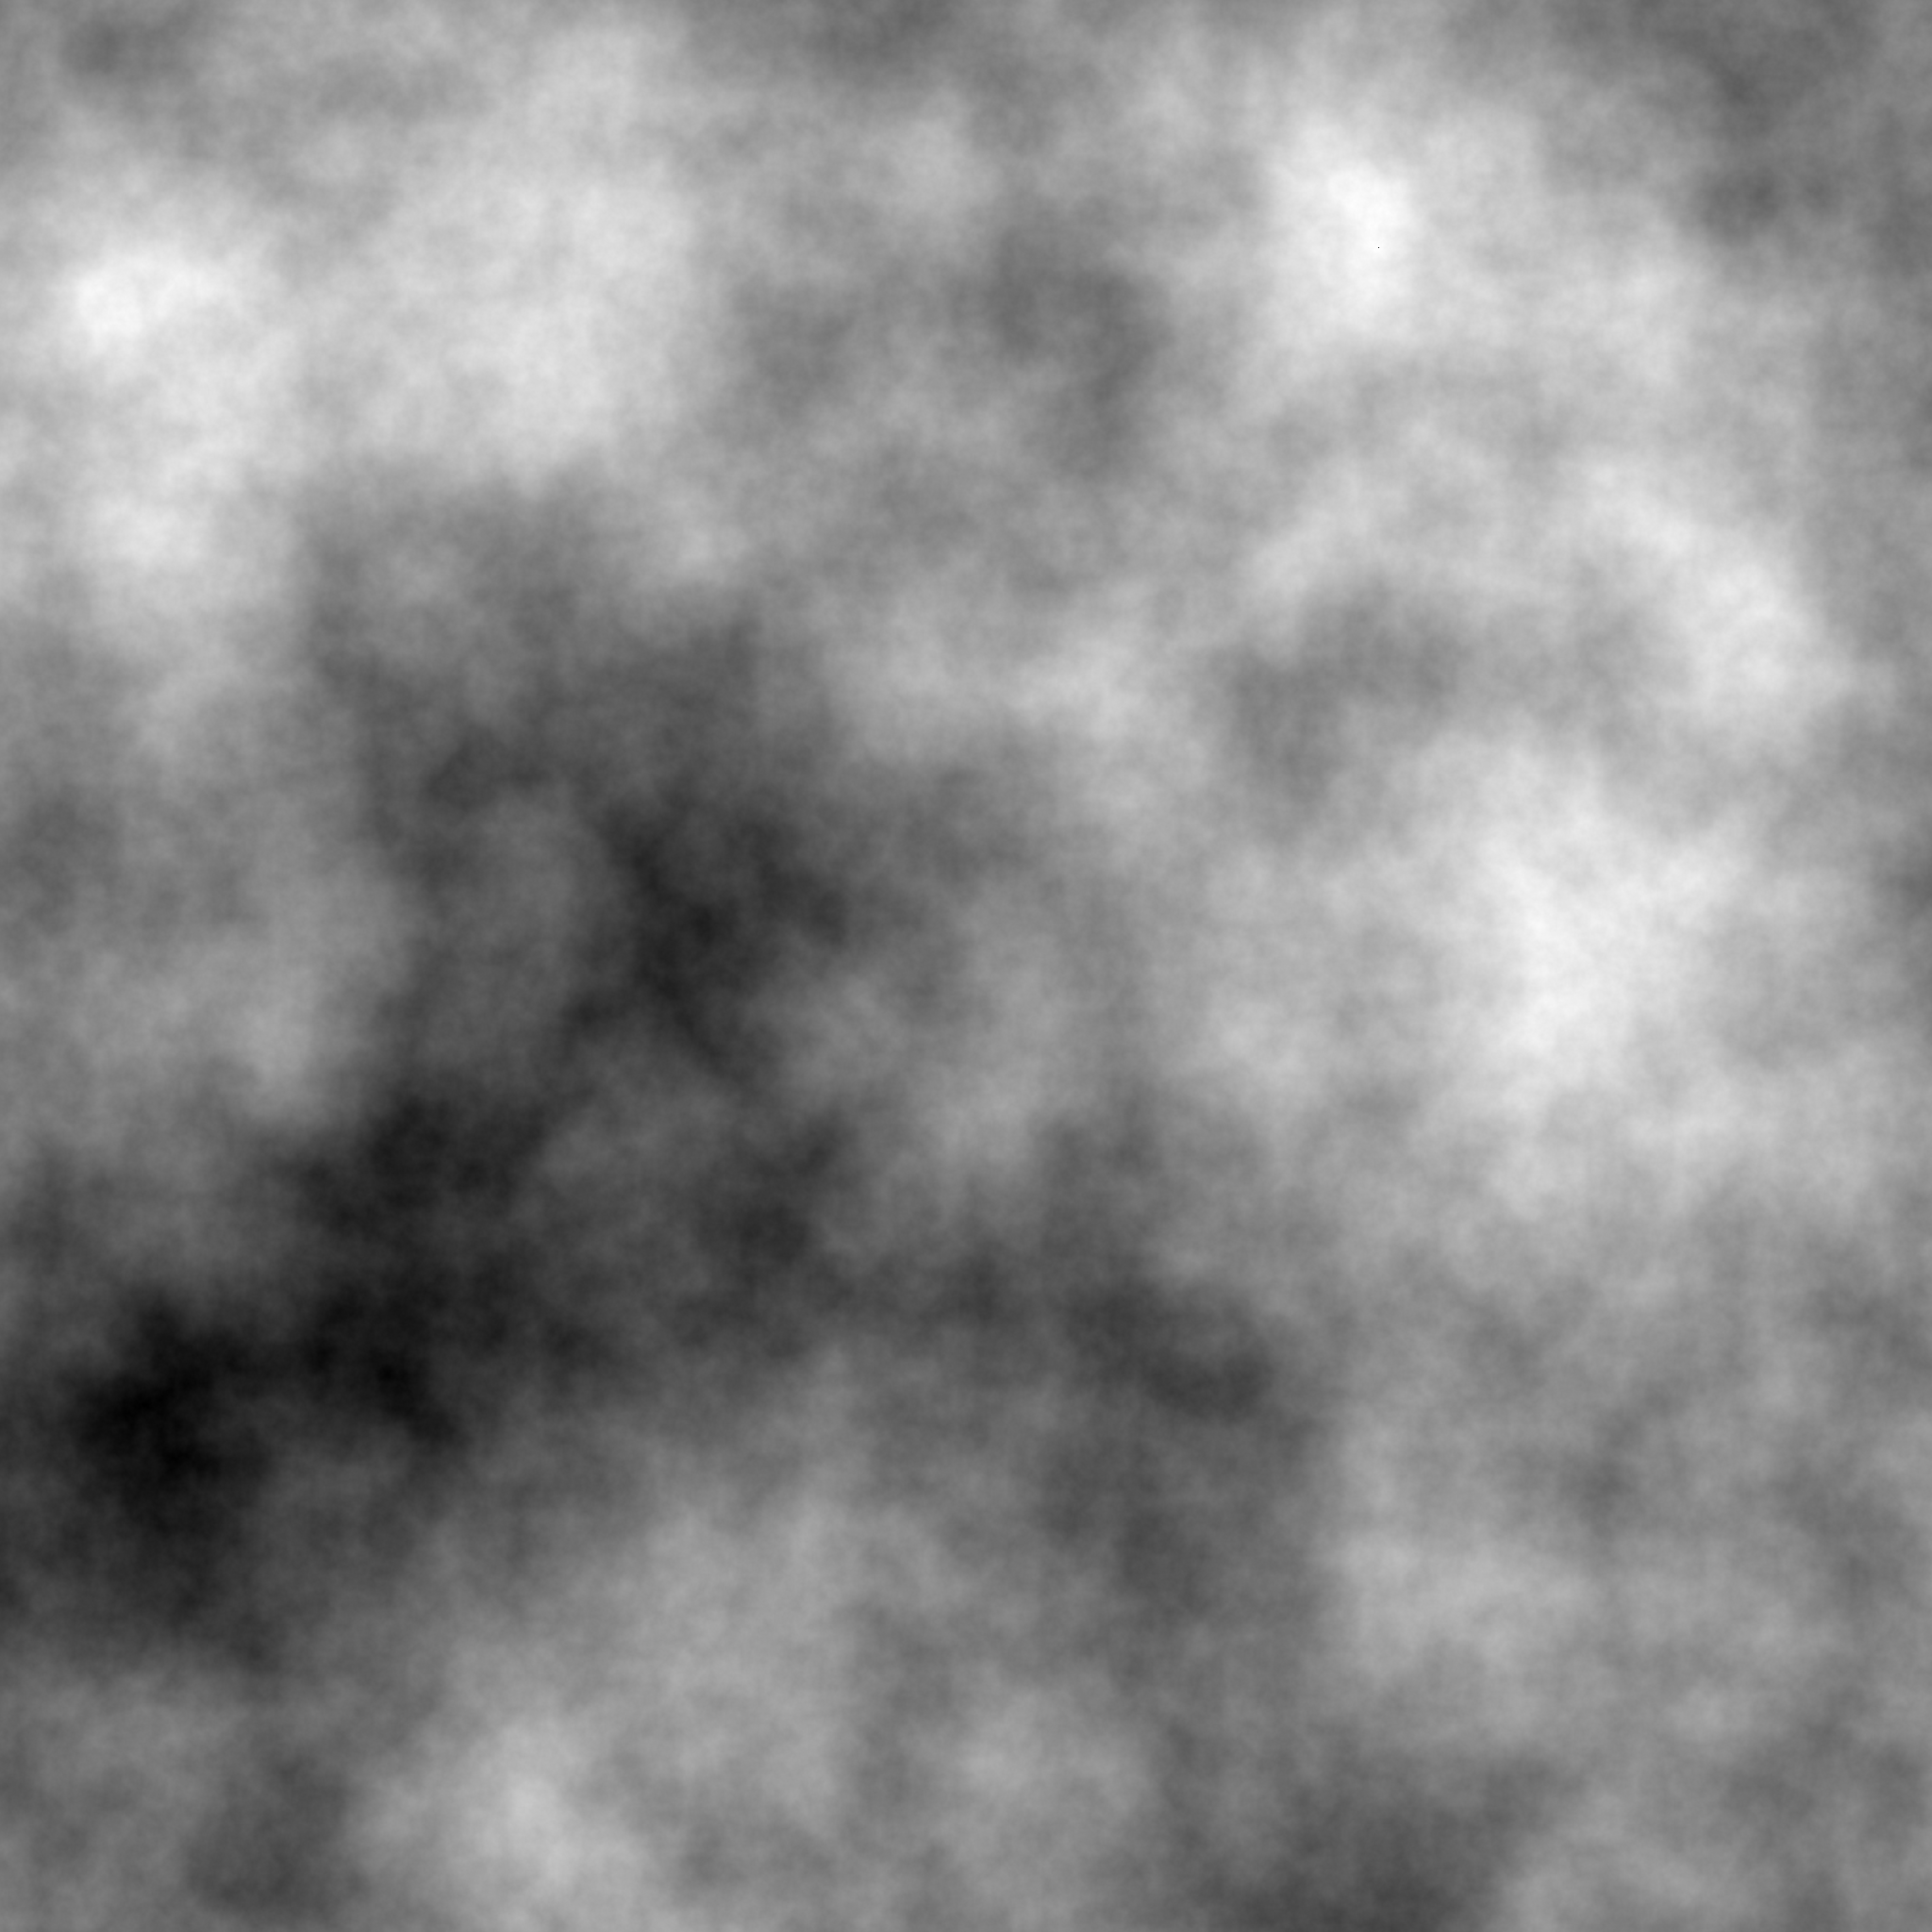
\includegraphics[width=0.4\textwidth]{data/perlin_comb_render_heightmap.png}
  \hskip 1cm
  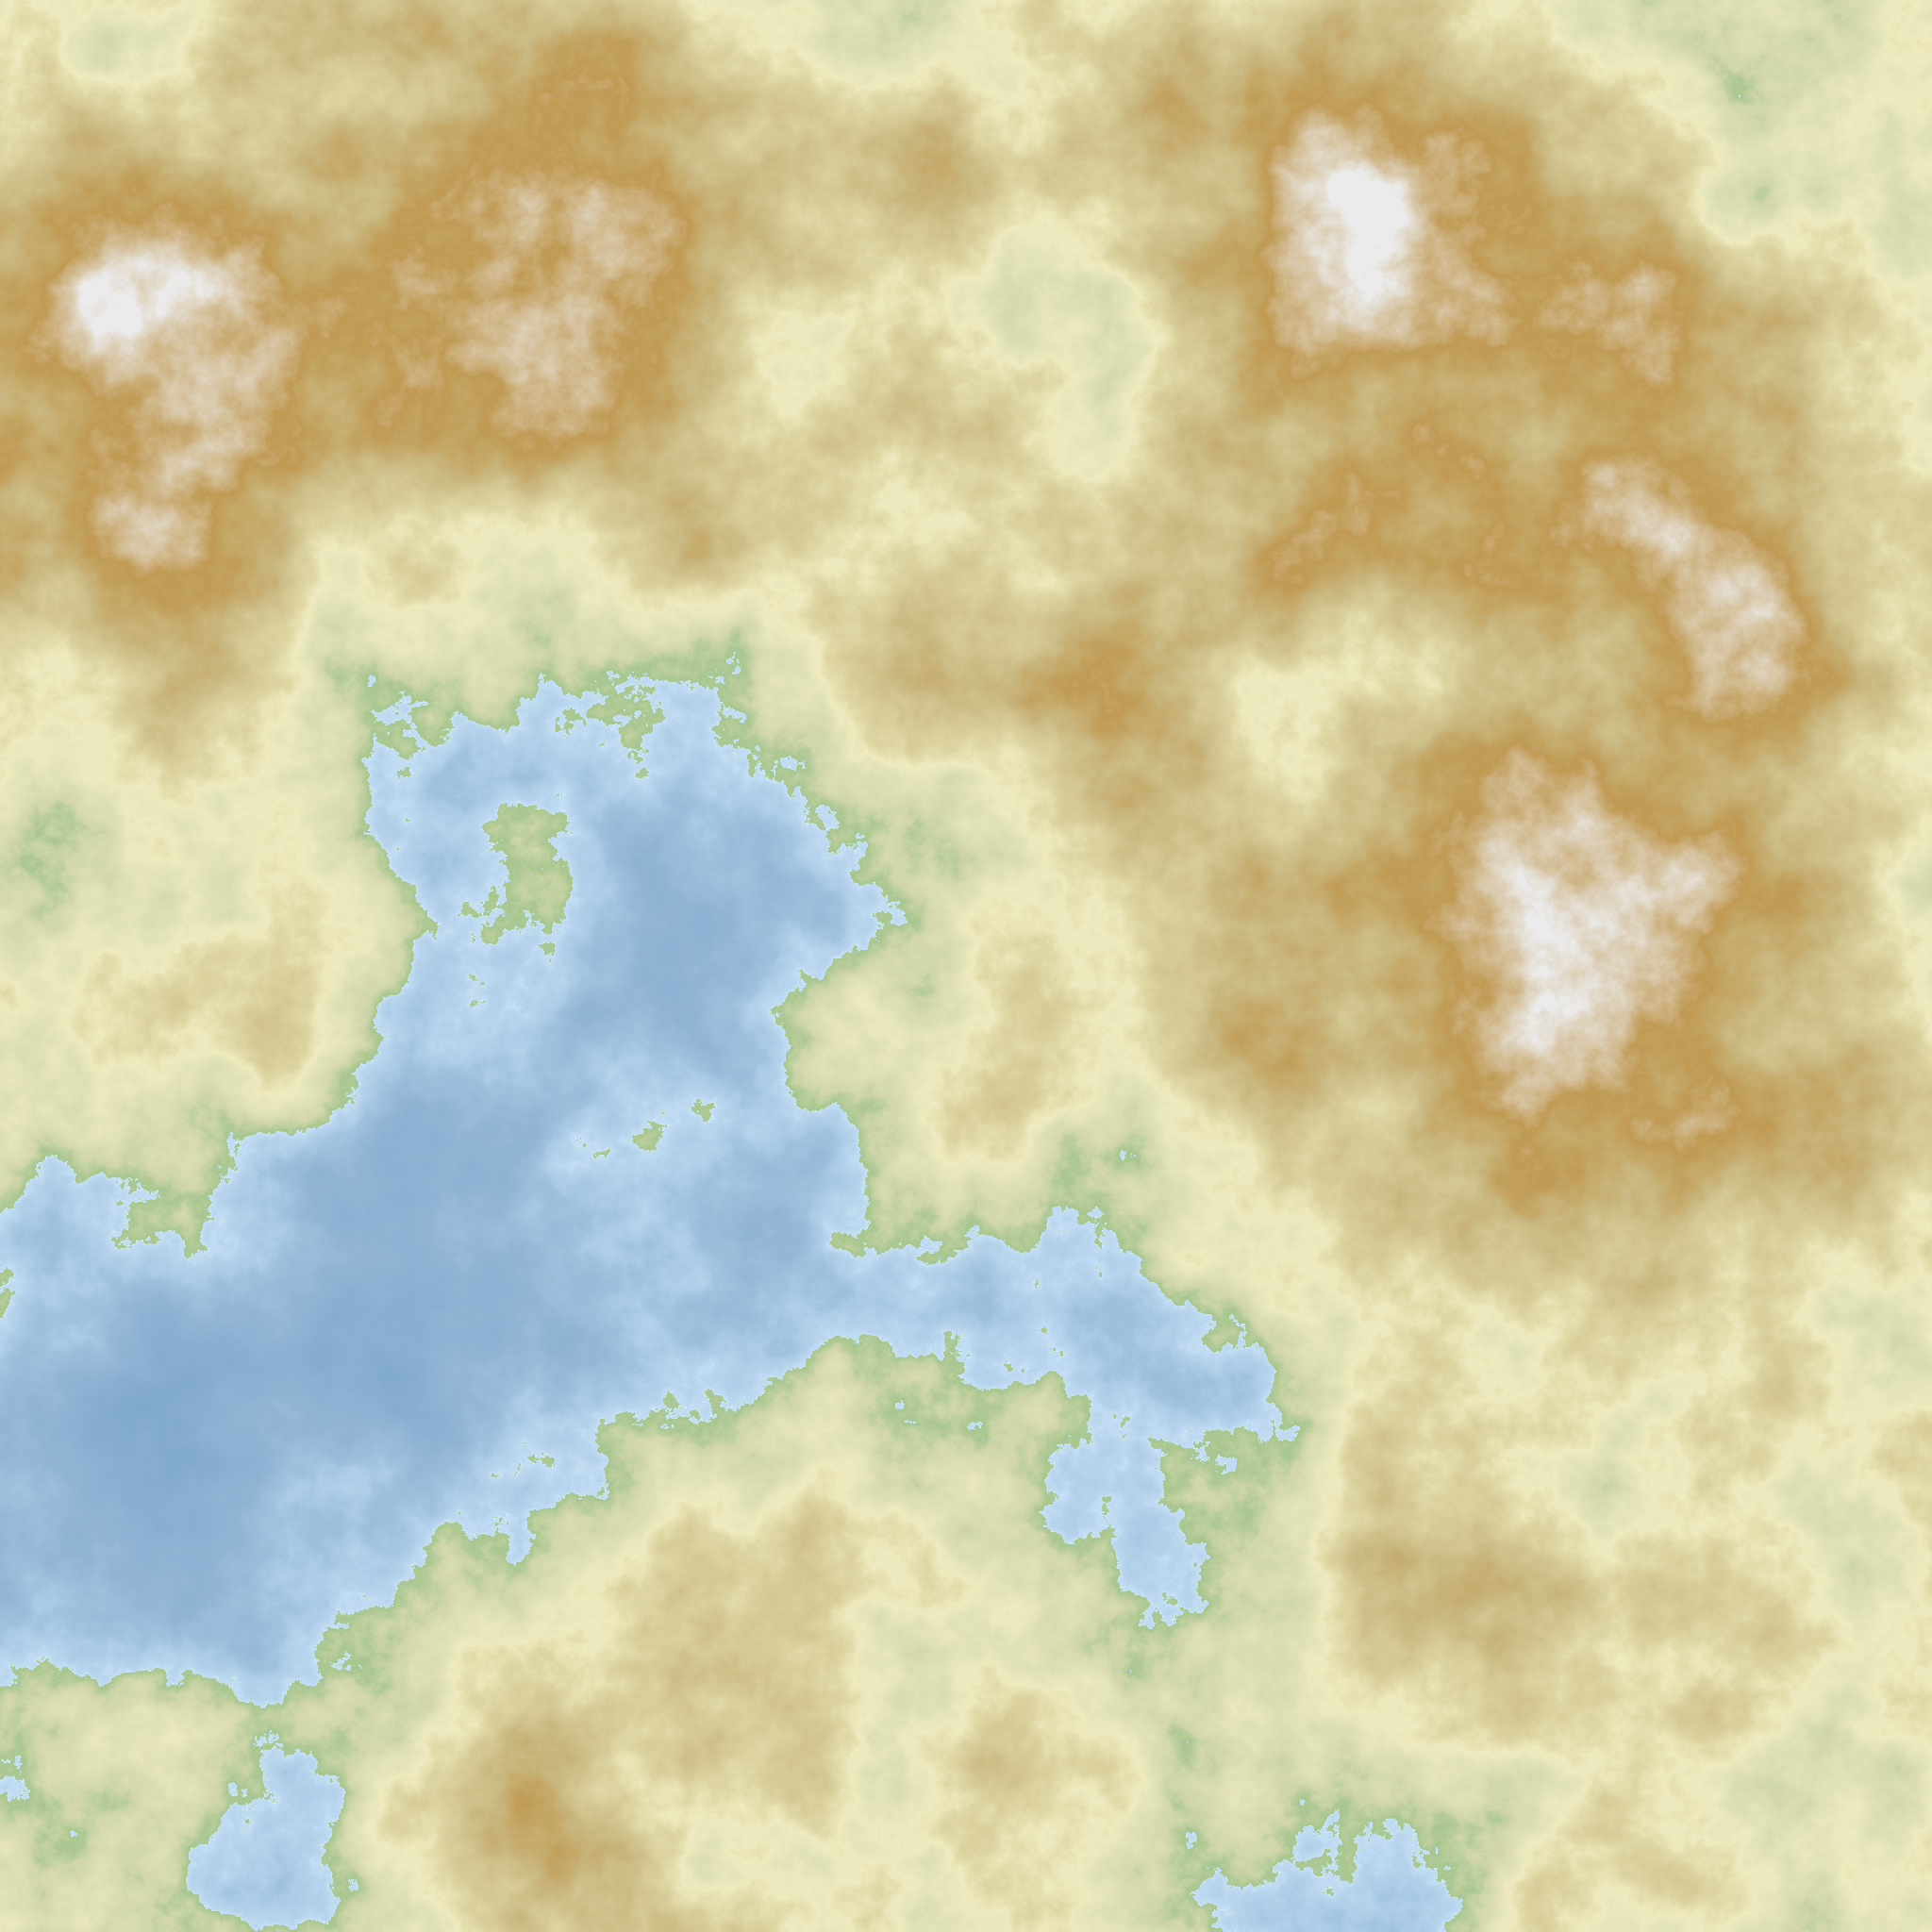
\includegraphics[width=0.4\textwidth]{data/perlin_comb_render_colored.png}
}

 
Teraz bude treba zafarbený obrázok vytieňovať. Na to použijeme jednoduchý osvetľovací model\indexItem{Alg}{Lambertov osvetľovací model}
(tzv. Lambertov). Predstav si, že máš malú plôšku, ktorá má normálový vektor $\vec n$
a nejakú základnú farbu. Čím na ňu dopadá menej svetla, tým je tmavšia. Ako viem zistiť,
koľko svetla na ňu dopadá? Ak svetlo prichádza z nejakého smeru, pozriem sa na uhol
medzi zdrojom svetla s normálovým vektorom:\\
  
\centerline{
%\tikzset{external/force remake}
%\tdplotsetmaincoords{50}{45}
%\begin{tikzpicture}[tdplot_main_coords]
\begin{tikzpicture}[x={(1,0)}, z={(0,1)}, y={(0.5,0.5)}]
  \def\dot[#1](#2){\fill[fill=#1] (#2) circle (1.2pt) ;}
  \def\sun(#1,#2,#3){
    \begin{scope}[canvas is xz plane at y=#2]
      \begin{scope}[shift={(#1,#3)},every path/.style={fill=white,draw=orange,very thick}]
        \filldraw (0,0) circle (0.2cm);
      \def\n{20}  
        \foreach \i in {0,...,\n} {
          \pgfmathsetmacro{\tmp}{\i*360/\n}
        \draw (\tmp:0.3cm) -- (\tmp:0.4cm);
        }
    \end{scope}
    \end{scope}
  }

  \def\ax{2}\def\ay{1}\def\az{2}
  \def\sx{0}\def\sy{0}\def\sz{5}
  \def\ux{1}\def\uy{4}\def\uz{0}
  \def\vx{-1}\pgfmathsetmacro{\vy}{1.0/\uy}\def\vz{0.6}

  \coordinate (Ax) at (\ax,\ay,0);
  \coordinate (h) at (0,0,\az);

  \coordinate (S) at (\sx,\sy,\sz);

  
  \normalize{\ux}{\uy}{\uz}
  \normalize{\vx}{\vy}{\vz}
  \coordinate (u) at (\ux,\uy,\uz);
  \coordinate (v) at (\vx,\vy,\vz);
  \coordinate (A) at ($(Ax)+(h)$);
  \def\s{1}
  \coordinate (P) at ($(A)-\s*(u) - \s*(v)$);
  \cross{\nx}{\ny}{\nz}{\ux}{\uy}{\uz}{\vx}{\vy}{\vz}

  \normalize{\nx}{\ny}{\nz}
  \coordinate (n) at (\nx,\ny,\nz);

  \begin{scope}[canvas is xy plane at z=0]
    \draw [gray!50, thin] (-1,-1) grid (4,4);
  \end{scope}
  \draw[orange,thick,dotted] (\sx,\sy,0)  -- (S);
  \dot[orange](\sx,\sy,0)
 
  \coordinate (u2) at (\ux,\uy,0);
  \coordinate (v2) at (\vx,\vy,0);
  \coordinate (P2) at ($(Ax)-\s*(u2)-\s*(v2)$);


  \filldraw[fill=green!10] (P) -- ($(P)+2*\s*(u)$) --($(P)+2*\s*(u)+2*\s*(v)$) -- 
  ($(P)+2*\s*(v)$) -- cycle;
  \draw[green!50!black,thick,dotted](Ax)--($(A)+(0,0,0)$);

  \coordinate (An) at ($(A)+1.5*(n)$);
  \draw[draw=none]  pic[draw, angle radius=4ex] {angle = An--A--S};

  \draw[orange,thick,->,shorten >= 3ex] (A)--node[anchor=south west]{$\vec s$}(S);
  \draw[teal,thick,->] (A)--(An) node[anchor=west]{$\vec n$};
  \dot[green!50!black](A);
  \dot[green!50!black](Ax);
  \sun(\sx,\sy,\sz)
  \node[above=1ex] at (A) {$\alpha$};

  %\drawaxes
\end{tikzpicture}}


Kosínus tohoto uhla mi vyjadruje množstvo dopadajúceho svetla: ak plôška smeruje presne na zdroj svetla, uhol je $0$,
$\cos(0)=1$, takže farba je najsilnejšia. Ako uhol rastie, $\cos(\alpha)$ postupne klesá, až keď je uhol $90^\circ$,
tak nedopadá žiadne svetlo $\cos(90^\circ)=0$.
Ak $\vec s$ je vektor smerom k svetelnému zdroju, stačí mi znormalizovať ho
a vyrátať skalárny súčin s $\vec n$ a mám $\cos(\alpha)$, ktorý potrebujem.


Posledná otvorená otázka je, ako vyrátať normálový vektor pre nejaký pixel
vo výškovej mape. Môžem to spraviť napríklad tak, že sa pozriem na 8 okolitých pixelov. Každý z nich mi dáva trojuholník,
ktorému viem vypočítať normálový vektor pomocou vektorového súčinu. Výsledný vektor potom dostanem ako priemer 
normálových vektorov trojuholníkov:\\


\centerline{
%\tikzset{external/force remake}
%\tdplotsetmaincoords{50}{45}
%\begin{tikzpicture}[tdplot_main_coords]
\begin{tikzpicture}[x={(1,0)}, z={(0,1)}, y={(0.25,0.5)}, scale=3.2]
  \def\dot[#1](#2){\fill[fill=#1] (#2) circle (0.4pt) ;}

  \begin{scope}[canvas is xy plane at z=0]
    \draw [gray!50, thin] (-0.5,-0.5) grid (2.5,2.5);
  \end{scope}

  \def\vaa{0.9}
  \def\vab{1.0}
  \def\vac{1.4}

  \def\vba{1.1}
  \def\vbb{1.2}
  \def\vbc{1.3}
  
  \def\vca{0.2}
  \def\vcb{0.6}
  \def\vcc{0.4}

  \def\chval#1{\if#10a\else\if#11b\else c\fi\fi}
  \def\w#1#2{\csname v\chval#1\chval#2\endcsname}
  \def\crd#1#2{#1,#2,\w{#1}{#2}}

  \coordinate (O) at (1,1,\w11);

  \coordinate (N) at (0,0,0);

  \foreach \i/\j/\ii/\jj/\f in {
    0/2/1/2/0%
    ,1/2/2/2/0%
    ,0/1/0/2/0%
    ,2/2/2/1/0%
    ,0/0/0/1/0%
    ,1/0/0/0/1%
    ,2/1/2/0/0%
    ,2/0/1/0/0%
  } {
    \draw[dotted] (\i,\j,0)--(\crd{\i}{\j}) (\ii,\jj,0) -- (\crd{\ii}{\jj});
    \filldraw[thin,gray,fill=yellow!10, opacity=0.6](\crd{\i}{\j})--(\crd{\ii}{\jj})--(\crd11)--cycle;

    \coordinate (A) at (\crd{\i}{\j});
    \coordinate (B) at (\crd{\ii}{\jj});
    \coordinate (P) at ($0.33*(A)+0.33*(B)+0.33*(O)$);
    \dot[blue](P)
    \pgfmathsetmacro{\ux}{\ii-1}
    \pgfmathsetmacro{\uy}{\jj-1}
    \pgfmathsetmacro{\uz}{\w{\ii}{\jj}-\w11}
    \pgfmathsetmacro{\vx}{\i-1}
    \pgfmathsetmacro{\vy}{\j-1}
    \pgfmathsetmacro{\vz}{\w{\i}{\j}-\w11}
    \cross{\nx}{\ny}{\nz}{\ux}{\uy}{\uz}{\vx}{\vy}{\vz}
    \normalize{\nx}{\ny}{\nz}
    \typeout{(\ux,\uy,\uz) x (\vx,\vy,\vz) =(nrm) (\nx,\ny,\nz)}
    \coordinate (n) at (\nx,\ny,\nz);
    \draw[blue,->](P)--($(P)+0.3*(n)$);
    \coordinate (N) at ($(N)+(n)$);
    \if\f1
      \draw[thick,red,->](O)--node[anchor=east]{$\vec u$}(A);
      \draw[thick,magenta,->](O)--node[anchor=north west, pos=0.6]{$\vec v$}(B);
    \fi
  }
  \coordinate (O) at (\crd11);
  \draw[thick,teal,->] (O) -- ($(O)+0.125*(N)$) node[above]{$\vec n$};

  \foreach \i in {0,1,2}{
    \foreach \j in {0,1,2} {
      \dot[black](\crd{\i}{\j})
    }}

    
  \draw[gray,brace=0.1ex/mirror] (0,0,0)--node[below=1.2ex]{$s$}(1,0,0);

  %\drawaxes
\end{tikzpicture}}


Naprogramovať sa to dá napríklad takto:


\begin{lstlisting}
Vec3 normala(Tabulka<double> &H, int i, int j, double s = 1) {
  Vec3 res;
  vector<Vec> dir{{0, 1},   {1, 1},  {1, 0},  {1, -1}, {0, -1},
                  {-1, -1}, {-1, 0}, {-1, 1}, {0, 1}};
  for (int t = 0; t < dir.size() - 1; t++) {
    int i0 = i + dir[t].x,     j0 = j + dir[t].y, 
        i1 = i + dir[t + 1].x, j1 = j + dir[t + 1].y;
    res +=
        -1.0 *
        (
         (Vec3{s * dir[t].x, s * dir[t].y, H(i0, j0)} 
          - Vec3{0, 0, H(i, j)}) 
          ^ // vektorový súčin
         (Vec3{s * dir[t + 1].x, s * dir[t + 1].y, H(i1, j1)} -
          Vec3{0, 0, H(i, j)})
        );
  }
  return res.normalize();
}
\end{lstlisting}


Táto funkcia dostane ako parameter tabuľku \vb{H} a pozíciu pixela \vb{i,j}.
Navyše dostanem parameter \vb{s}, ktorý hovorí, ako ďaleko sú od seba jednotlivé pixely
(t.j. výškovú mapu si predstavujem ako sieť s krokom \vb{s}).


Pre obrázok s rozmermi $2048\times2048$ som si nastavil smer svetla na 
\prg!Vec3 light{-1, 1, 12};! a \prg!double s=0.004;! a 
z výškovej mapy \vb{H} som si vyrátal tabuľku \prg!Tabulka<double> N!
takto:

\begin{lstlisting}
light.normalize();
for (int i = 0; i < H.m; i++)
  for (int j = 0; j < H.n; j++)
    if (H(i, j) <= wl)
      N(i, j) = 1;
    else
      N(i, j) = light * normala(H, i, j, s);
\end{lstlisting}


Výsledok je na obrázku vľavo. Obrázok vpravo vznikol tak, že som každú farbu pixela na ofarbenej mape
prenásobil koeficientom\footnote{%
t.j. zobral som $60\%$ pôvodnej farby a $40\%$ som rozdelil od čiernej po pôvodnú farbu
podľa normály. Nie je to úplne ideálne, ale môže nám to postačiť.
}  \prg!0.6 + 0.4 * max(0.0, N(i, j));!\\


\centerline{
  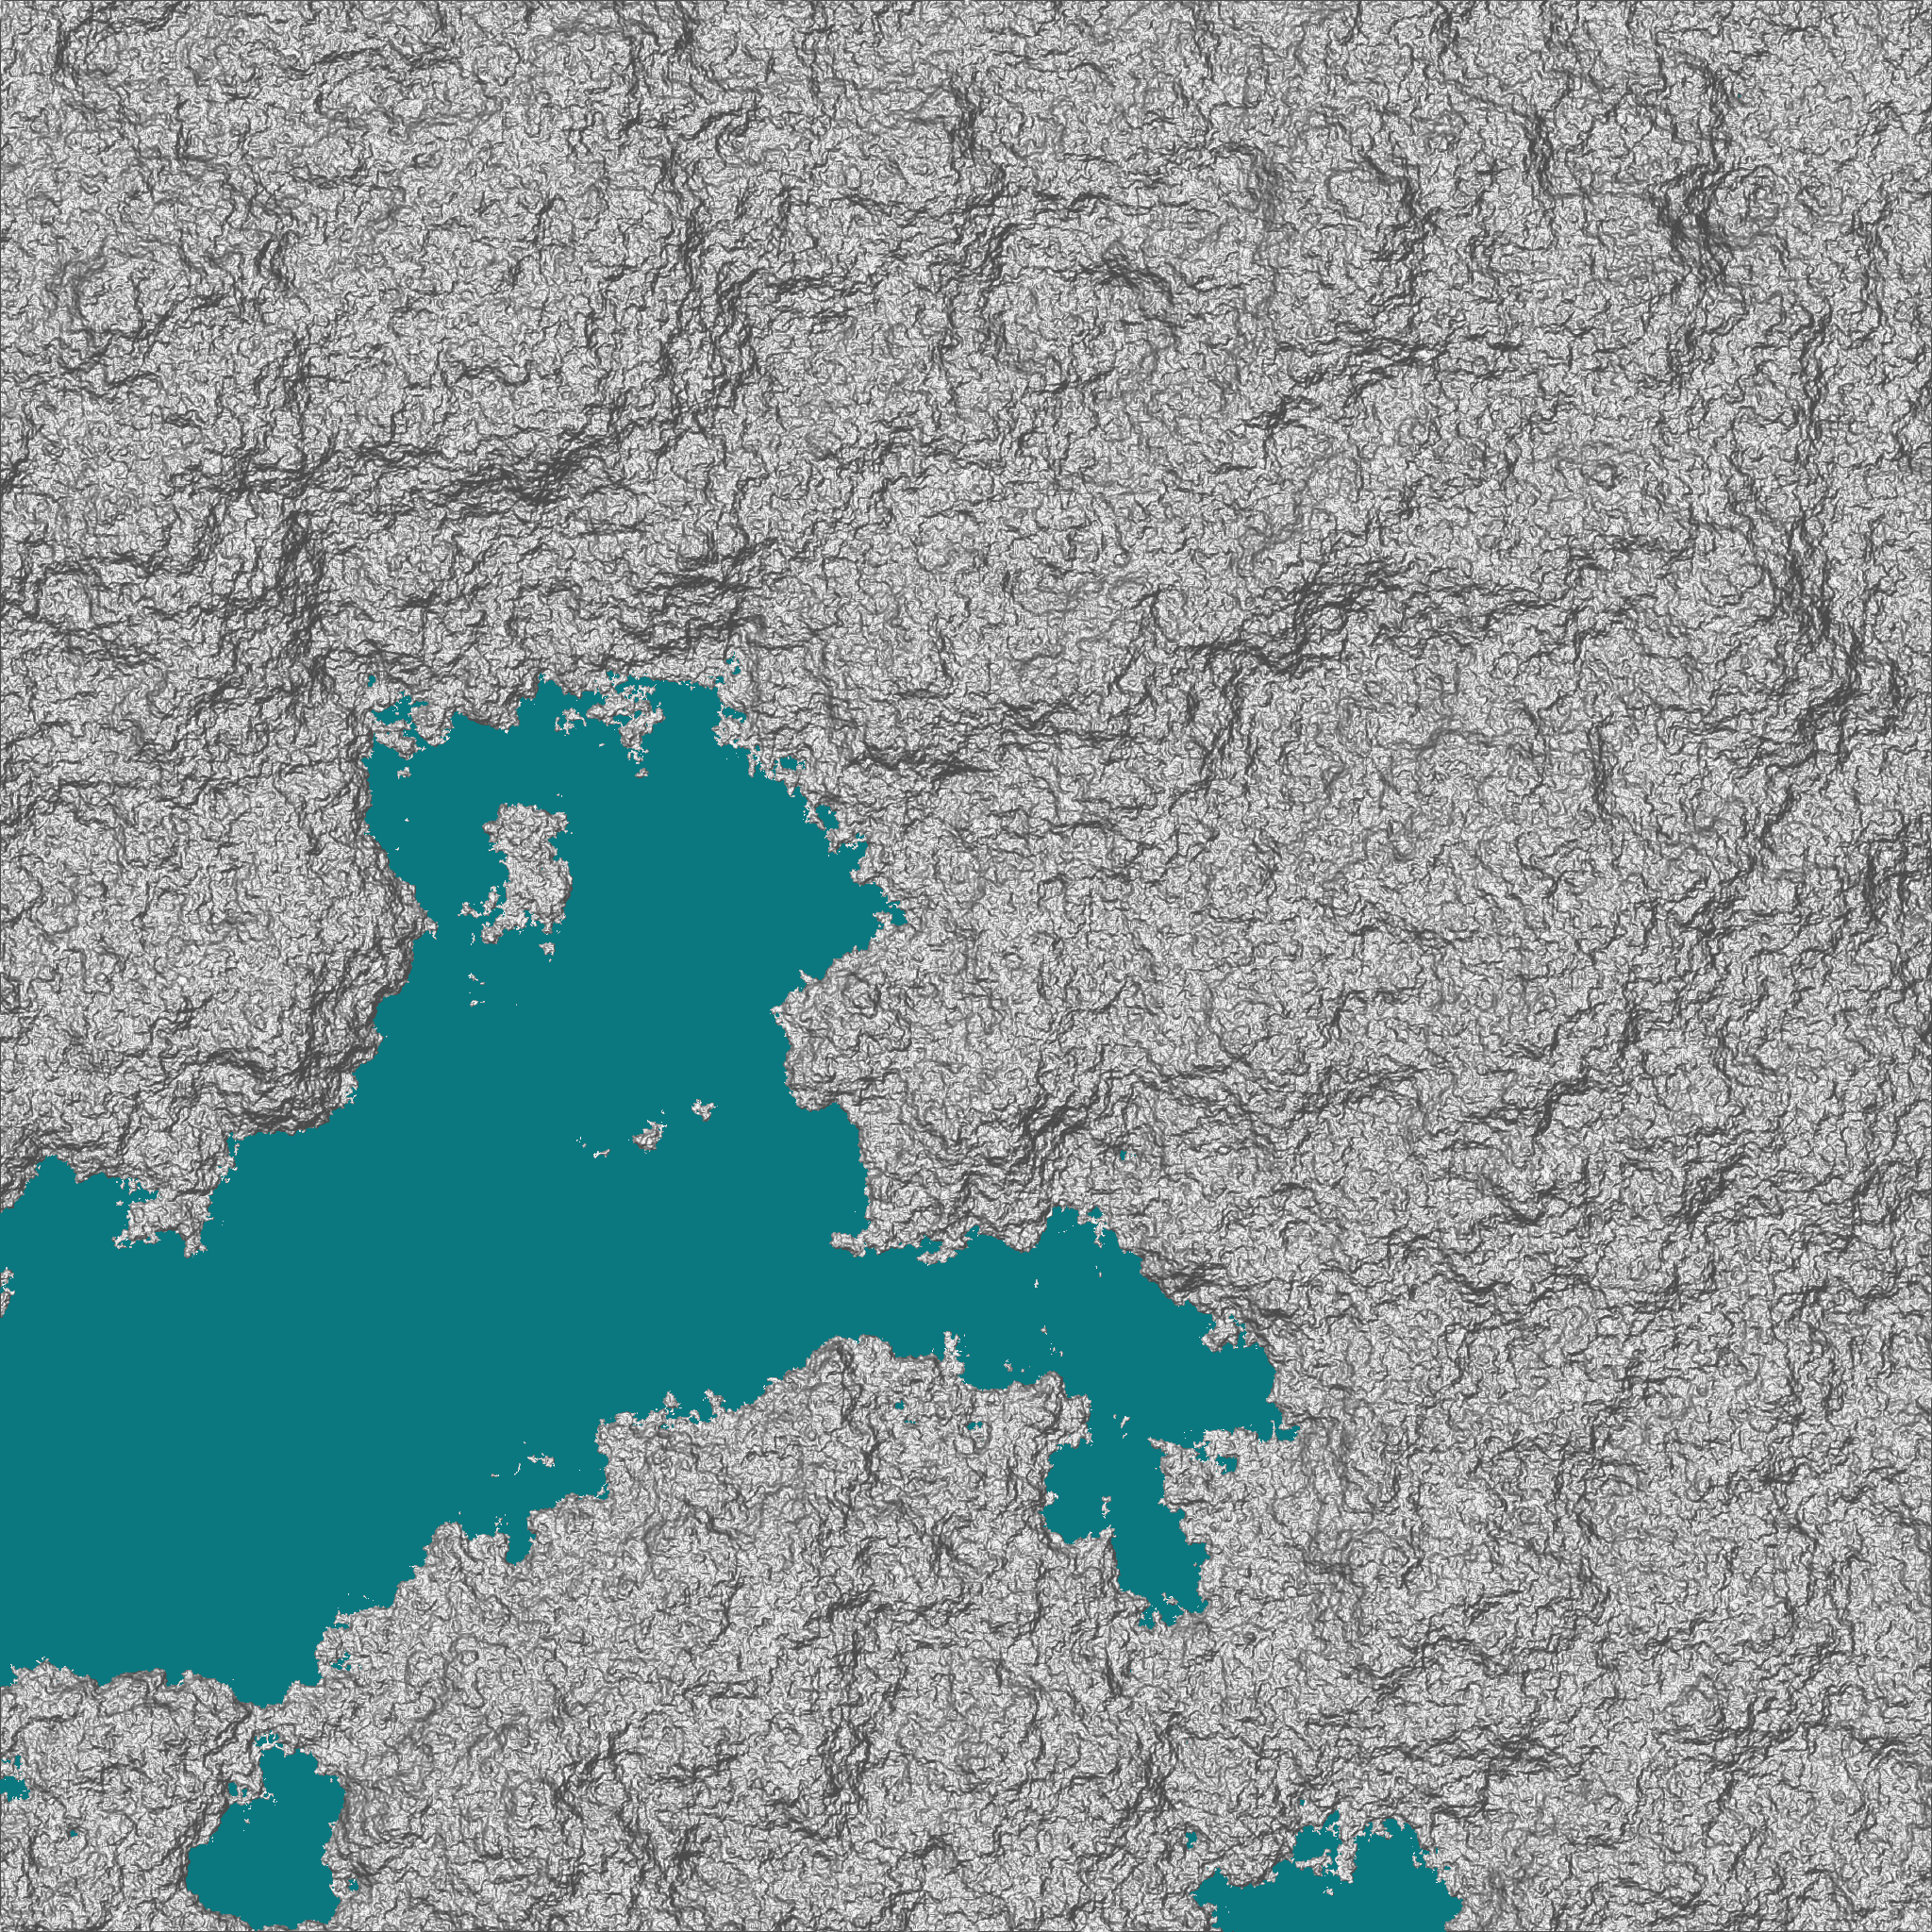
\includegraphics[width=0.4\textwidth]{data/perlin_comb_render_normal.png}
  \hskip 1cm
  \includegraphics[width=0.4\textwidth]{data/perlin_comb_render_rendered.png}
}


Toto už vyzerá ako mapa terénu, aj keď zrovna ostrov to nie je. To sa dá ale ľahko napraviť pri generovaní
výškovej mapy: okrem Perlinovho šumu sa navyše každý bod posunie dole úmerne jeho vzdialenosti od stredu 
obrázka. Okraje klesnú a v strede ostane ostrov. S trochou hrania sa s klesaním okrajov
a zvýraznením hôr som dospel k takémuto
výsledku:\\


\centerline{
  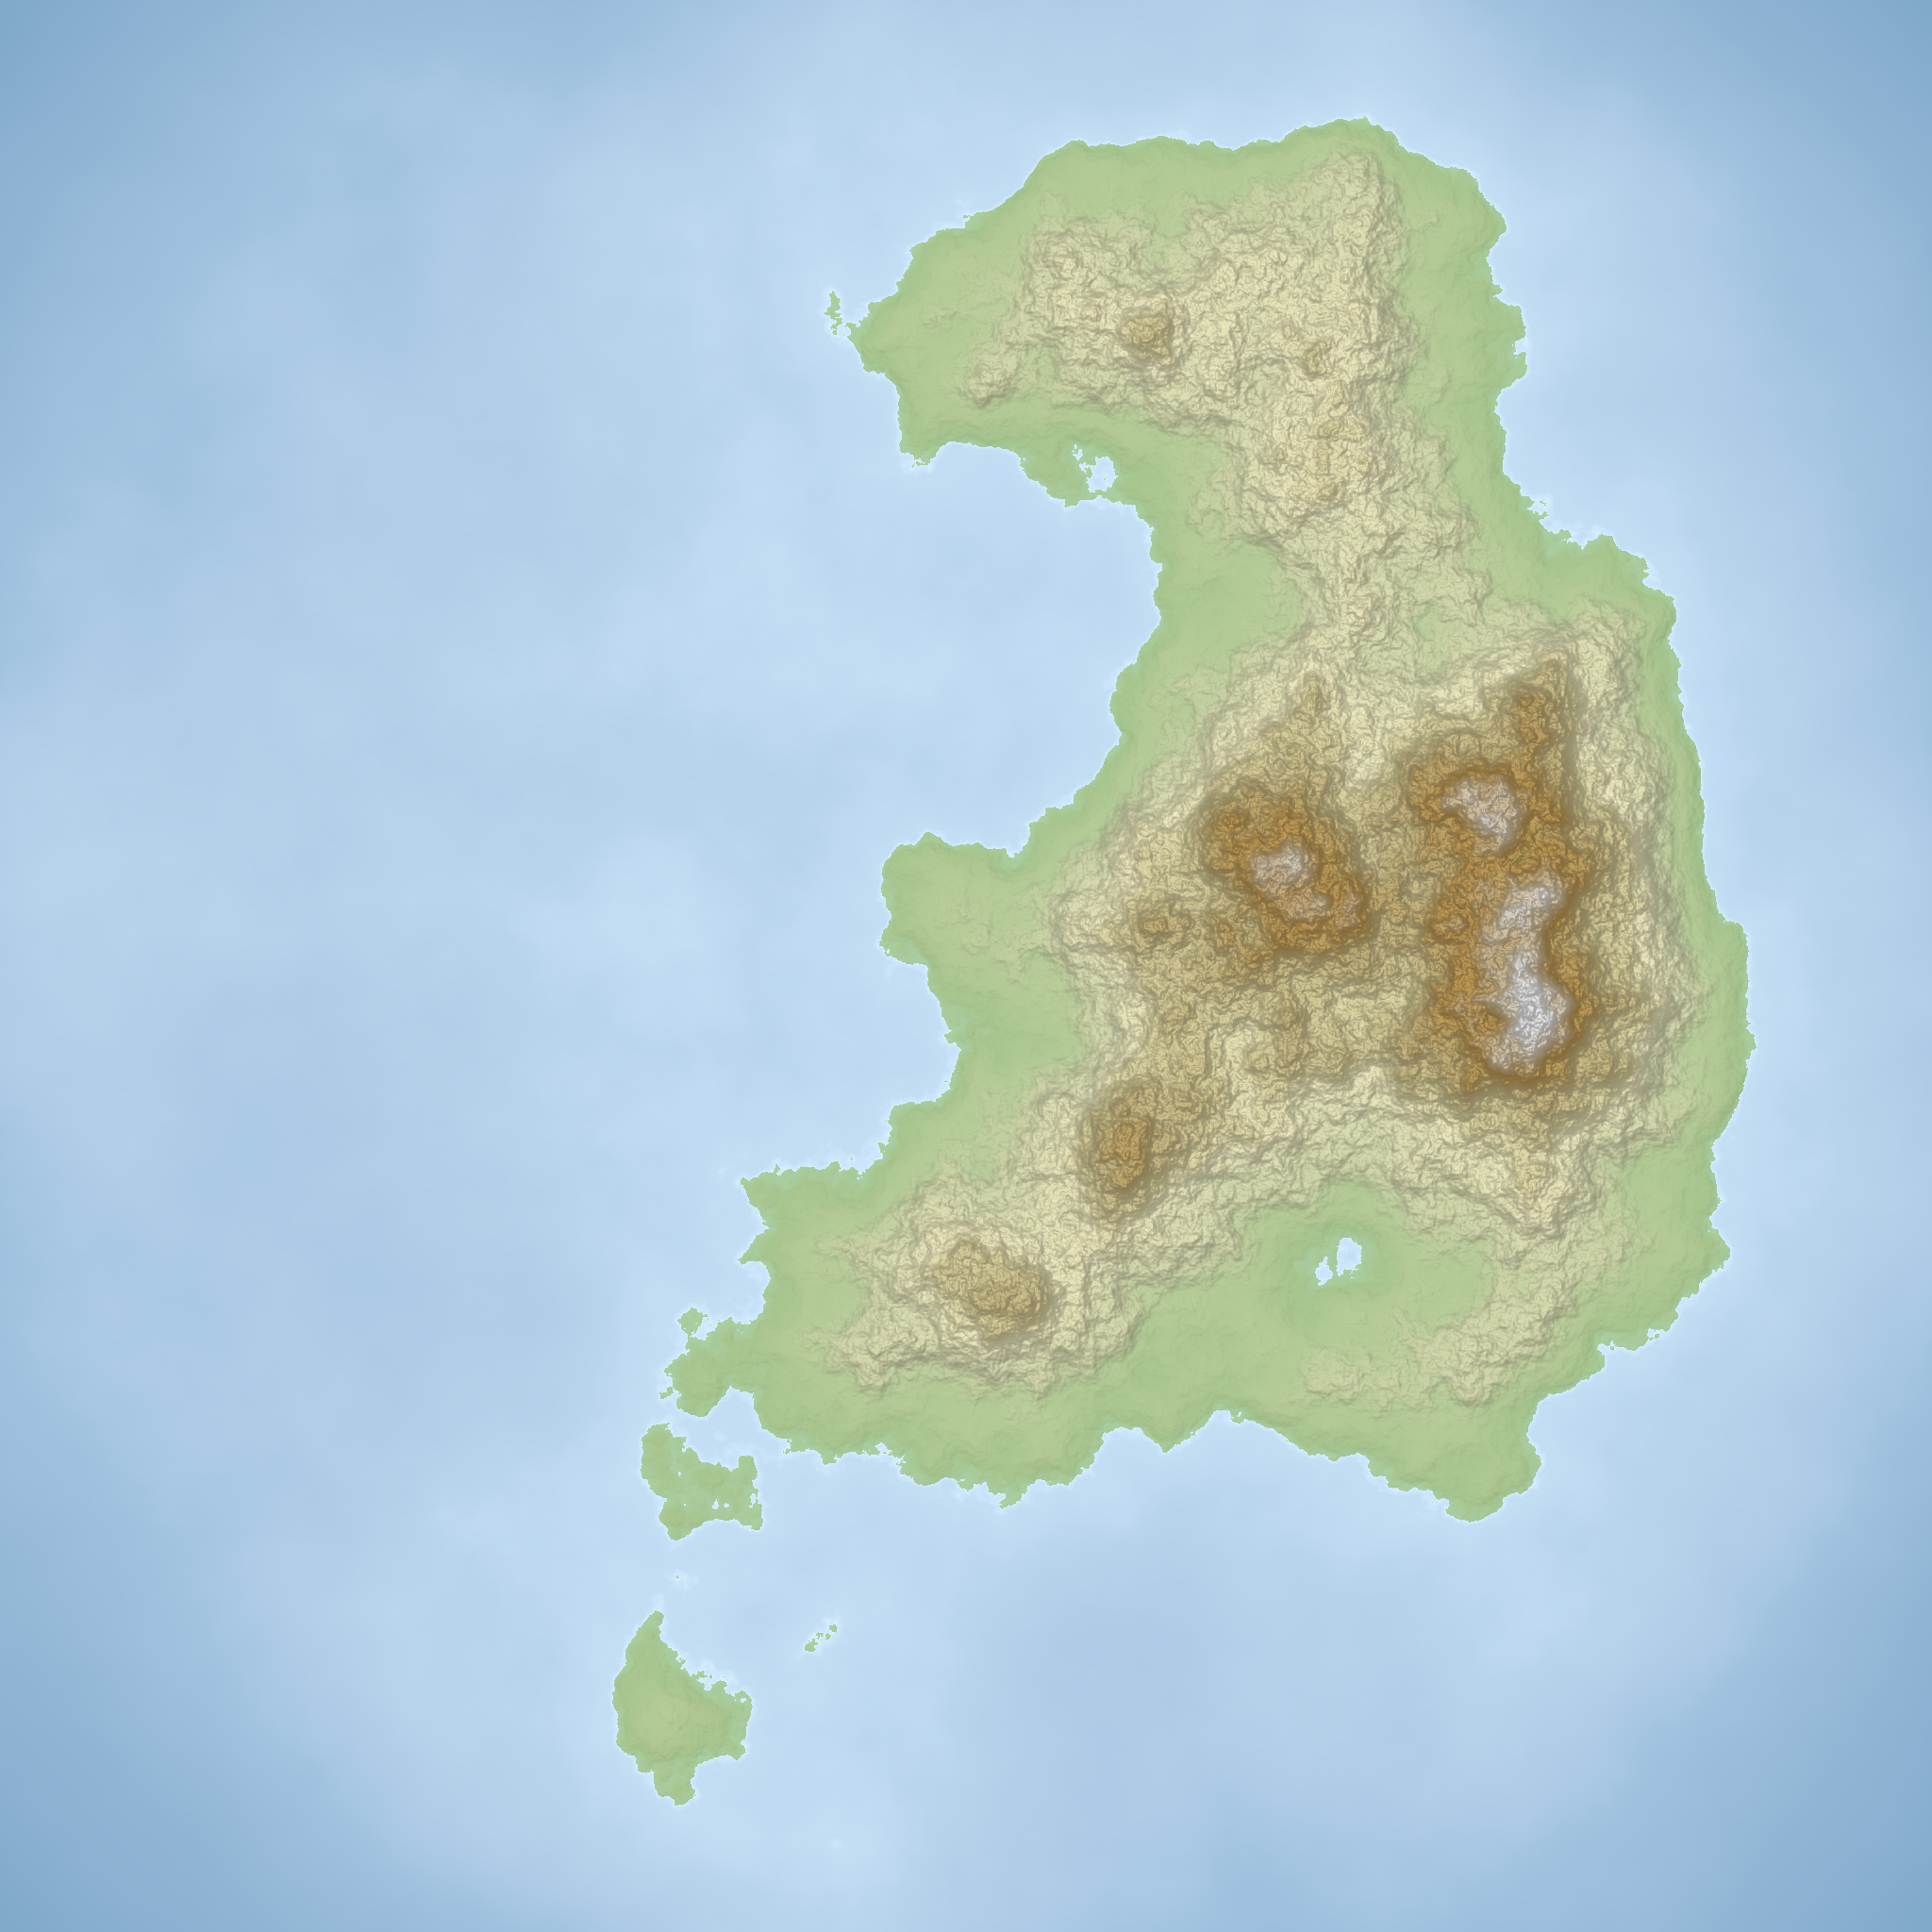
\includegraphics[width=0.7\textwidth]{data/86_rendered_dry.png}
}


Úplne posledná vec, ktorá tomu chýba, sú doliny riek a fjordy. Rozhodol som sa preto spraviť jednoduchú\indexItem{Alg}{simulácia erózie}
fyzikálnu simuláciu vodnej erózie. Urobiť realistickú virtuálnu eróziu je téma sama osebe, ale 
v \link%
{https://www.firespark.de/resources/downloads/implementation\%20of\%20a\%20methode\%20for\%20hydraulic\%20erosion.pdf}%
{bakalárskej práci Hansa Beyera}
je veľmi zjednodušený a ľahko naprogramovateľný prístup, ktorý si tu môžeme vyskúšať.
Hlavná idea je, že na povrch našej výškovej mapy budeme púšťať kvapky\footnote{
  Vzhľadom na mierku, ktorú máme, to bude skôr ako futbalový štadión plný vody, ale
  volajme to kvapka.}. Kvapka má nejaký objem vody a v nej je rozpustený nejaký objem 
bahna. Ak je bahna málo a kvapka ide rýchlo, vymyje kúsok z povrchu: výšková mapa sa trochu 
zníží a v kvapke bude viac bahna. Naopak, ak je bahna veľa a kvapka ide pomaly, bahno sa bude
usadzovať: v kvapke ho ostane menej a povrch sa trochu zvýši.
Ako zistíme, ktorým smerom sa bude kvapka pohybovať? Krátka odpoveď je, že v smere, ktorým
ukazuje normálový vektor. Dalo by sa to pomerne jednoducho spočítať, ale nateraz sa uspokojme
s intuitívnou predstavou podľa obrázka




\centerline{
%\tikzset{external/force remake}
%\tdplotsetmaincoords{50}{45}
%\begin{tikzpicture}[tdplot_main_coords]
\begin{tikzpicture}[x={(1,0)}, z={(0,1)}, y={(0.5,0.5)}]
%\begin{tikzpicture}[x={(1,0)}, z={(0,0)}, y={(0,1)}]
  \def\dot[#1](#2){\fill[fill=#1] (#2) circle (1.2pt) ;}

  \def\rotplane[#1][#2][#3]{ %zxz
  \begin{scope}[canvas is xy plane at z=0]
    \draw [gray!20, very thin] (-1.5,-1.5) grid (1.5,1.5);
  \end{scope}
    \def\h{1}
    \def\d{1}
    \pgfmathsetmacro{\ax}{-0.5*\d}\pgfmathsetmacro{\ay}{-0.5*\d}\pgfmathsetmacro{\az}{0}
    \pgfmathsetmacro{\bx}{0.5*\d}\pgfmathsetmacro{\by}{-0.5*\d}\pgfmathsetmacro{\bz}{0}
    \pgfmathsetmacro{\cx}{0.5*\d}\pgfmathsetmacro{\cy}{0.5*\d}\pgfmathsetmacro{\cz}{0}
    \pgfmathsetmacro{\dx}{-0.5*\d}\pgfmathsetmacro{\dy}{.5*\d}\pgfmathsetmacro{\dz}{0}
    \pgfmathsetmacro{\nx}{0}\pgfmathsetmacro{\ny}{0}\pgfmathsetmacro{\nz}{1}

    \rotz[#1]{\ax}{\ay}{\az}
    \rotz[#1]{\bx}{\by}{\bz}
    \rotz[#1]{\cx}{\cy}{\cz}
    \rotz[#1]{\dx}{\dy}{\dz}
    \rotz[#1]{\nx}{\ny}{\nz}

    \rotx[#2]{\ax}{\ay}{\az}
    \rotx[#2]{\bx}{\by}{\bz}
    \rotx[#2]{\cx}{\cy}{\cz}
    \rotx[#2]{\dx}{\dy}{\dz}
    \rotx[#2]{\nx}{\ny}{\nz}

    \rotz[#3]{\ax}{\ay}{\az}
    \rotz[#3]{\bx}{\by}{\bz}
    \rotz[#3]{\cx}{\cy}{\cz}
    \rotz[#3]{\dx}{\dy}{\dz}
    \rotz[#3]{\nx}{\ny}{\nz}

    \begin{scope}[shift={(0,0,\h)}]
      \filldraw[fill=teal!20, opacity=0.6]  (\ax,\ay,\az) -- (\bx,\by,\bz) -- (\cx,\cy,\cz) -- (\dx,\dy,\dz) -- cycle;
    \draw[->] (0,0,0) -- (\nx,\ny,\nz);
    \dot[black](0,0,0);
    \end{scope}

    \draw[dashed] (0,0,0) -- (0,0,\h);
    \draw[->,magenta] (0,0,0) -- (\nx,\ny,0);

  }


  \rotplane[0][45][0]
  \begin{scope}[shift={(2,0)}]
    \rotplane[0][45][90]
  \end{scope}
  \begin{scope}[shift={(4,0)}]
    \rotplane[30][40][60]
  \end{scope}
  \begin{scope}[shift={(6,0)}]
    \rotplane[210][320][45]
  \end{scope}


  %\drawaxes
\end{tikzpicture}}


\phantomsection\label{page:gradient}
Predstav si malú plôšku, z ktorej trčí normálový vektor ako klinec. Ktorým smerom klincom
pohneš, tým smerom sa plôška nakloní, a tade bude aj kvapka padať. Takže stačí nám
zrátať normálový vektor v 3D a pozrieť sa na jeho priemet, t.j. na zložky v smere $x$
a $y$. Výsledný 2D vektor sa volá {\em gradient} a udáva smer, ktorým plôška klesá. 


Pre účely simulácie si budeme pozíciu kvapky pamätať v reálnych číslach ako
premennú \prg!Vec pos!. Výšková mapa mi bude udávať výšku v bodoch s celočíselnými
súradnicami (tieto budem volať {\em mrežové body}).
Pre danú pozíciu si skutočnú výšku vyrátame bilineárnou interpoláciou zo 
štyroch susedných mrežových bodov. Normálu vyrátam podobne -- najprv vyrátam normálové 
vektory v štyroch susedných mrežových bodoch a výsledok zrátam bilineárnou interpoláciou.\\



\centerline{
%\tikzset{external/force remake}
\begin{tikzpicture}[x={(1,0)}, z={(0,0.7)}, y={(0.25,0.5)}, scale=4]
%\begin{tikzpicture}[x={(1,0)}, z={(0,0)}, y={(0,1)}, scale=3.5]
  \def\dot[#1](#2){\fill[fill=#1] (#2) circle (0.4pt) ;}

  \begin{scope}[canvas is xy plane at z=0]
    \draw [gray!50, thin] (-0.2,-0.2) grid (1.2,1.2);
  \end{scope}

  \def\vs{0.5}
  \def\newv(#1)#2#3#4{
    \def\tmpx{#2}
    \def\tmpy{#3}
    \def\tmpz{#4}
    \normalize{\tmpx}{\tmpy}{\tmpz}
    \coordinate (#1) at (\vs*\tmpx,\vs*\tmpy,\vs*\tmpz);
    \coordinate (#1!0) at (\vs*\tmpx,\vs*\tmpy,0);
  }
  \def\chval#1{\if#10a\else\if#11b\else\if#12c\else d\fi\fi\fi}
  \def\w#1#2{\csname v\chval#1\chval#2\endcsname}
  \def\crd#1#2{#1,#2,\w{#1}{#2}}

  \def\vaa{1.0} \newv(n00){-0.2}{-0.3}{1}
  \def\vab{1.3} \newv(n01){-0.2}{-0.7}{1.5}

  \def\vba{0.8} \newv(n10){-0.2}{-0.3}{1}
  \def\vbb{1.5} \newv(n11){-0.2}{-0.7}{1} 
  
  \foreach \i in {0,1}{
    \foreach \j in {0,1} {
      \coordinate (A\i\j) at (\crd{\i}{\j});
      \coordinate (A\i\j!0) at (\i,\j,0);
    }}


  \def\px{0.5} \def\py{0.7}


  \coordinate (P!0) at (\px,\py,0);
  \coordinate (P0!0) at (\px,0,0);
  \coordinate (P1!0) at (\px,1,0);

  \coordinate (P0) at ($(A00)!\px!(A10)$);
  \coordinate (P1) at ($(A01)!\px!(A11)$);
  \coordinate (P) at ($(P0)!\py!(P1)$);

  \foreach \a in {0,1}{
  \coordinate (nP\a) at ($(n0\a)!\px!(n1\a)$);
  \coordinate (nP\a!0) at ($(n0\a!0)!\px!(n1\a!0)$);
  }
  \coordinate (nP) at ($(nP0)!\py!(nP1)$);
  \coordinate (nP!0) at ($(nP0!0)!\py!(nP1!0)$);

  \filldraw[fill=yellow!10, opacity=0.3] (A00) -- (A10) -- (A11) -- (A01) -- cycle;

  \draw[thin,dashed,gray] (P) -- (P!0);

  \foreach \a in {0,1}{
  \draw[magenta,->] (P\a)--($(P\a)+(nP\a)$);
  \draw[magenta!30,->](P\a!0)--($(P\a!0)+(nP\a!0)$);
  }
  \draw[magenta, dotted] (P0)--(P1);
  \draw[magenta!30, dotted] (P0!0)--(P1!0);
  \draw[magenta,thick, ->] (P)--($(P)+(nP)$) node[above] {\vb{norm}};
  \draw[magenta,thick,->](P!0)--($(P!0)+(nP!0)$) node[anchor = north east]  {\vb{g}};

  %\draw let \p1=(nP0!0),\p2=(n00!0),\p3=(n10!0) in (2,0) node{\x1,\y1 :: \x2,\y2 :: \x3,\y3};
  




  \foreach \i in {0,1}{
    \foreach \j in {0,1} {
      \draw[teal,->] (A\i\j) -- ($(A\i\j)+(n\i\j)$);
      \draw[cyan,->] (A\i\j!0) -- ($(A\i\j!0)+(n\i\j!0)$);

      \dot[black](A\i\j)
      \draw[dashed,gray,thin] (A\i\j!0) -- (A\i\j);
    }}

    \dot[black](P!0);
    \node[anchor=north west] at (P!0) {\vb{pos}};
    
  \foreach \p in {P,A00!0,A11!0} {
  \dot[black](\p)
  }

  \node[anchor=north west] at (P) {\vb{vyska(pos)}};


  \node[anchor = south east] at (A00!0) {\vb{(ix, iy)}};   
  \node[anchor = north west ] at (A11!0) {\vb{(ix + 1, iy + 1)}};   

  %\drawaxes
\end{tikzpicture}}



Simulácia jednej kvapky bude vyzerať takto. Kvapka sa na začiatku zajví na náhodnej pozícii

\begin{lstlisting}
Vec pos{dis(rnd) * n, dis(rnd) * n};
\end{lstlisting}

Budeme simulovať niekoľko krokov, na
to budeme mať konštantu \vb{lifetime}. V každom kroku vyrátame gradient \prg!Vec g;!
tak, ako sme to práve opísali. Nový smer kvapky \prg!dir! získame tak, že interpolujeme
gradient a predchádzajúci smer s parametrom \vb{zotrvacnost}, t.j. budeme robiť
\prg!dir = lerp(g, dir, zotrvacnost);!. Výsledný smer normalizujeme tak, aby sa 
kvapka pohla o vzdialenosť jedna. 
Vyrátame pôvodnú výšku a novú výšku a 
ich rozdiel označíme \vb{delta}.


O kvapke si navyše pamätáme rýchlosť\footnote{%
  Rýchlosť používam iba pri výpočte erózie. Pri určovaní smeru sa vždy pohnem o jednotku.
  To je kvôli tomu, aby rýchle kvapky nepreskakovali mrežové body a pomalé kvapky sa zbytočne
  nesimulovali veľakrát na tom istom mieste.},
  objem vody (číslo od 0 do 1) a množstvo rozpusteného bahna.
 Koľko bahna sa z kvapky môže usadiť závisí od sklonu, rýchlosti a množstva vody:

 
 \centerline{
   \prg!double dasausadit =  max(-delta, min_sklon) * rychlost * voda * rozpustnost;!} 


Pričom \prg!min_sklon! a \prg!rozpustnost! sú konštanty, ktoré si na začiatku nejak nastavíme.
Teraz môžu nastať dva prípady: ak kvapka tečie dokopca, alebo nesie viac bahna, ako 
\prg!dasauasdit!, bahno sa bude usádzať. Ak tečie dokopca (t.j. $\vb{delta}>0$)
bahno sa snaží vyplniť rozdiel výšok, t.j. usadí sa \prg!min(delta, bahno)!. V opačnom
prípade sa usadí \prg!(bahno - dasausadit) * usadzanie;!, kde \vb{usadzanie} je opäť
ďalší parameter z rozsahu 0 až 1. 
Usadené bahno odrátame z bahna v kvapke a prirátame ho k výškovej mape.
Pri tom použijeme zase bilineárnu interpoláciu, t.j. ak množstvo usadeného mahna máme 
v premennej \vb{usadit}, 
tak do výškovej mapy \vb{H} rozdelíme usadeninu 
podľa pozície kvapky medzi meržovými bodmi tak,
že bližšie mrežové body dostanú viac a vzdialenejšie menej\footnote{
Nasledovný program je možno trochu neprehľadný, ale vyskúšaj si, čo znamená pre konkrétne 
mrežové body. Napr. pre \vb{dx=0}, \vb{dy=0} vyplynie, že \vb{H(ix,iy)}
dostane časť \vb{(1 - p.x) * (1 - p.y)}. Ak napr. \vb{p} je na pozícii \vb{(ix,iy)},
tak \vb{p.x} aj \vb{p.y} je 0 a všetok materiál ide do \vb{H(ix,iy)}. Ak by 
\vb{pos} bolo na opačnom konci na pozícii \vb{(ix+1, iy+1)}, tak do \vb{H(ix,iy)}
nejde nič. 
}:


\vbox{
\begin{lstlisting}
int ix = pos.x, iy = pos.y;     // mrežový bod po zaokrúhlení pozície
Vec p{pos.x - ix, pos.y - iy};  // pozícia v rámci gridu

for (int dx = 0; dx < 2; dx++)
  for (int dy = 0; dy < 2; dy++) {
    H(ix + dx, iy + dy) += usadit * (dx * p.x + (1 - dx) * (1 - p.x)) *
                           (dy * p.y + (1 - dy) * (1 - p.y));
  }
\end{lstlisting}
}


Ak sa bahno neusádza, tak nastáva erózia: časť materiálu z výškovej mapy sa presunie
do kvapky. Aká veľká časť sa uberie, kontroluje ďalší parameter \vb{erozia}.
Materiál budeme uberať nielen zo susedných mrežových bodov, ale
zo širšieho okolia, aby nevznikali príilš úzke a strmé kaňony:

\begin{lstlisting}
double urvat = min((dasausadit - bahno) * erozia, -delta);

// odoberie zo širšieho okolia podľa toho, ako sú nastavené váhy
for (int dx = 0; dx < 2 * r + 1; dx++)
  for (int dy = 0; dy < 2 * r + 1; dy++) {
    int i = ix - r + dx, j = iy - r + dy;
    double kusok = urvat * vahy[dx][dy];
    H(i, j) -= kusok;
    bahno += kusok;
  }
\end{lstlisting}



Pole \vb{vahy} bude ako ''štetec'' rozmerov $2\vb{r}+1\times2\vb{r}+1$, ktorý 
si doredu pripravíme tak, aby pokrýval okolie do vzdialenosti \vb{r}, 
v strede mal väčšie hodnoty ako na krajoch a dokopy mal súčet 1 takto (číslo 
v políčku je váha v percentách):\\



\centerline{\begin{tikzpicture}[scale=0.7]
  \def\r{4}
  
  \pgfmathtruncatemacro{\n}{2*\r}
  \foreach \dx [
    remember=\suma (initially 0),    
  ]in {0,...,\n}{
    \foreach\dy[
      remember=\sumb (initially \suma),
    ] in {0,...,\n}{
      \pgfmathsetmacro{\dist}{sqrt((\r-\dx)*(\r-\dx)+(\r-\dy)*(\r-\dy))/(\r+1)}
       \ifdim\dist pt<1.0pt\pgfmathsetmacro{\w}{1-\dist}\else\pgfmathsetmacro{\w}{0}\fi
       \pgfmathsetmacro{\sumb}{\sumb+\w}
       \xdef\suma{\sumb}
    }
    \xdef\pako{\suma}
  }

  \foreach \dx in {0,...,\n} {
    \foreach \dy in {0,...,\n} {
      \pgfmathsetmacro{\dist}{sqrt((\r-\dx)*(\r-\dx)+(\r-\dy)*(\r-\dy))/(\r+1)}
       \ifdim\dist pt<1.0pt\pgfmathsetmacro{\w}{1-\dist}\else\pgfmathsetmacro{\w}{0}\fi
       \pgfmathsetmacro{\tmp}{100*\w/\pako}
       \pgfmathtruncatemacro{\c}{\tmp/6*90}
       \fill[teal!\c](\dx,\dy) rectangle ++(1,1);
       \ifnum\c<50\def\c{100}\else\def\c{0}\fi
       \ifdim\tmp pt>0pt\node[black!\c] at (0.5+\dx,0.5+\dy) {{\scriptsize 
         \calc[precision=1]{\tmp}}};\fi
     }
   }

  \draw[teal] (0,0) grid (\n+1,\n+1);
\end{tikzpicture}}


To sa dá naprogramovať napr. takto:


\begin{lstlisting}
double sum = 0;
for (int dx = 0; dx < 2 * r + 1; dx++)
  for (int dy = 0; dy < 2 * r + 1; dy++) {
    // vzdialenosť od stredu
    double dist = sqrt((r - dx) * (r - dx) + (r - dy) * (r - dy)) / (r + 1);
    double w = 0;
    if (dist < 1) w = (1 - dist);
    vahy[dx][dy] = w;
    sum += w;
  }
for (int dx = 0; dx < 2 * r + 1; dx++)
  for (int dy = 0; dy < 2 * r + 1; dy++) vahy[dx][dy] /= sum;
\end{lstlisting}


Pozícia \prg![r][r]! je  presne v strede poľa, preto 
$\sqrt{(\vb{r}-\vb{dx})^2+(\vb{r}-\vb{dy})^2}$ je vzdialenosť políčka 
\prg![dx][dy]! od stredu. Vzdialenosť predelíme \vb{r + 1}, aby sme dostali kruh s 
polomerom 1. Pozície mimo kruhu budú mať hodnotu 0, pozície v kruhu hodnotu 
úmernú vzdialenosti od stredu. Nakoniec každú hodnotu vydelíme súčtom\footnote{
  To je typická finta ako zaručiť, že celkový súčet je 1. Ak mám čísla
  $a_1, a_2,\ldots a_n$ a označím $s=a_1+a_2+\cdots+a_n$, tak keď zoberiem čísla
  $b_1=\frac{a_1}{s}$, $b_2=\frac{a_2}{s}$, \ldots, $b_n=\frac{a_n}{s}$, tak 
  ich vzájomné relatívne veľkosti sa nezmenia, lebo som všetky vydelil rovnakým číslom,
  a ich súčet bude $b_1+\cdots+b_n=\frac{a_1}{s}+\cdots+\frac{a_n}{s}=
  \frac{1}{s}(a_1+\cdots+a_n)=\frac{s}{s}=1$.
}.


Nakoniec upravíme rýchlosť podľa fyzikou inšpirovaného vzťahu

\begin{lstlisting}
if (delta < 0) delta *= -1;
rychlost = sqrt(rychlost * rychlost + delta * gravitacia);
\end{lstlisting}

kde \vb{gravitacia} je parameter, a odparíme časť vody 
\prg!voda *= (1 - odparovanie)! kde \vb{odparovanie} je ešte iný parameter.

\begin{uloha}
  Naprogramuj triedu \vb{Eroder}, ktorá v konštruktore dostane referenciu na 
  výškovú mapu a má funkciu \vb{kvap}, ktorá na nej odsimuluje jednu kvapku.
\end{uloha}

Výhodou tejto metódy je, že je jednoduchá, nevýhodou je, že má strašne veľa parametrov,
ktoré treba správne nastaviť, ak má výsledok vyzerať dobre\footnote{
  V pôvodnej práci je ešte jedno odporúčanie: keďže pri úpravách výškovej mapy sú zmeny
  pri jednej kvapke veľmi malé, kvôli reprezentácii reálnych čísel môže prísť
  k podtečeniu: číslo, ktoré prirátavame je tak malé, že sa v mantise neprejaví.
  Preto je lepšie udržovať
  si zmeny v separátnej tabuľke a až nakoniec ich prirátať k výškovej mape.}.


Po troche hrania sa s parametrami som dostal výsledok, s ktorým som bol viac-menej spokoný.
Na obrázku vľavo sú dráhy kvapiek, vpravo je ostrov po erózii.\\


\centerline{
  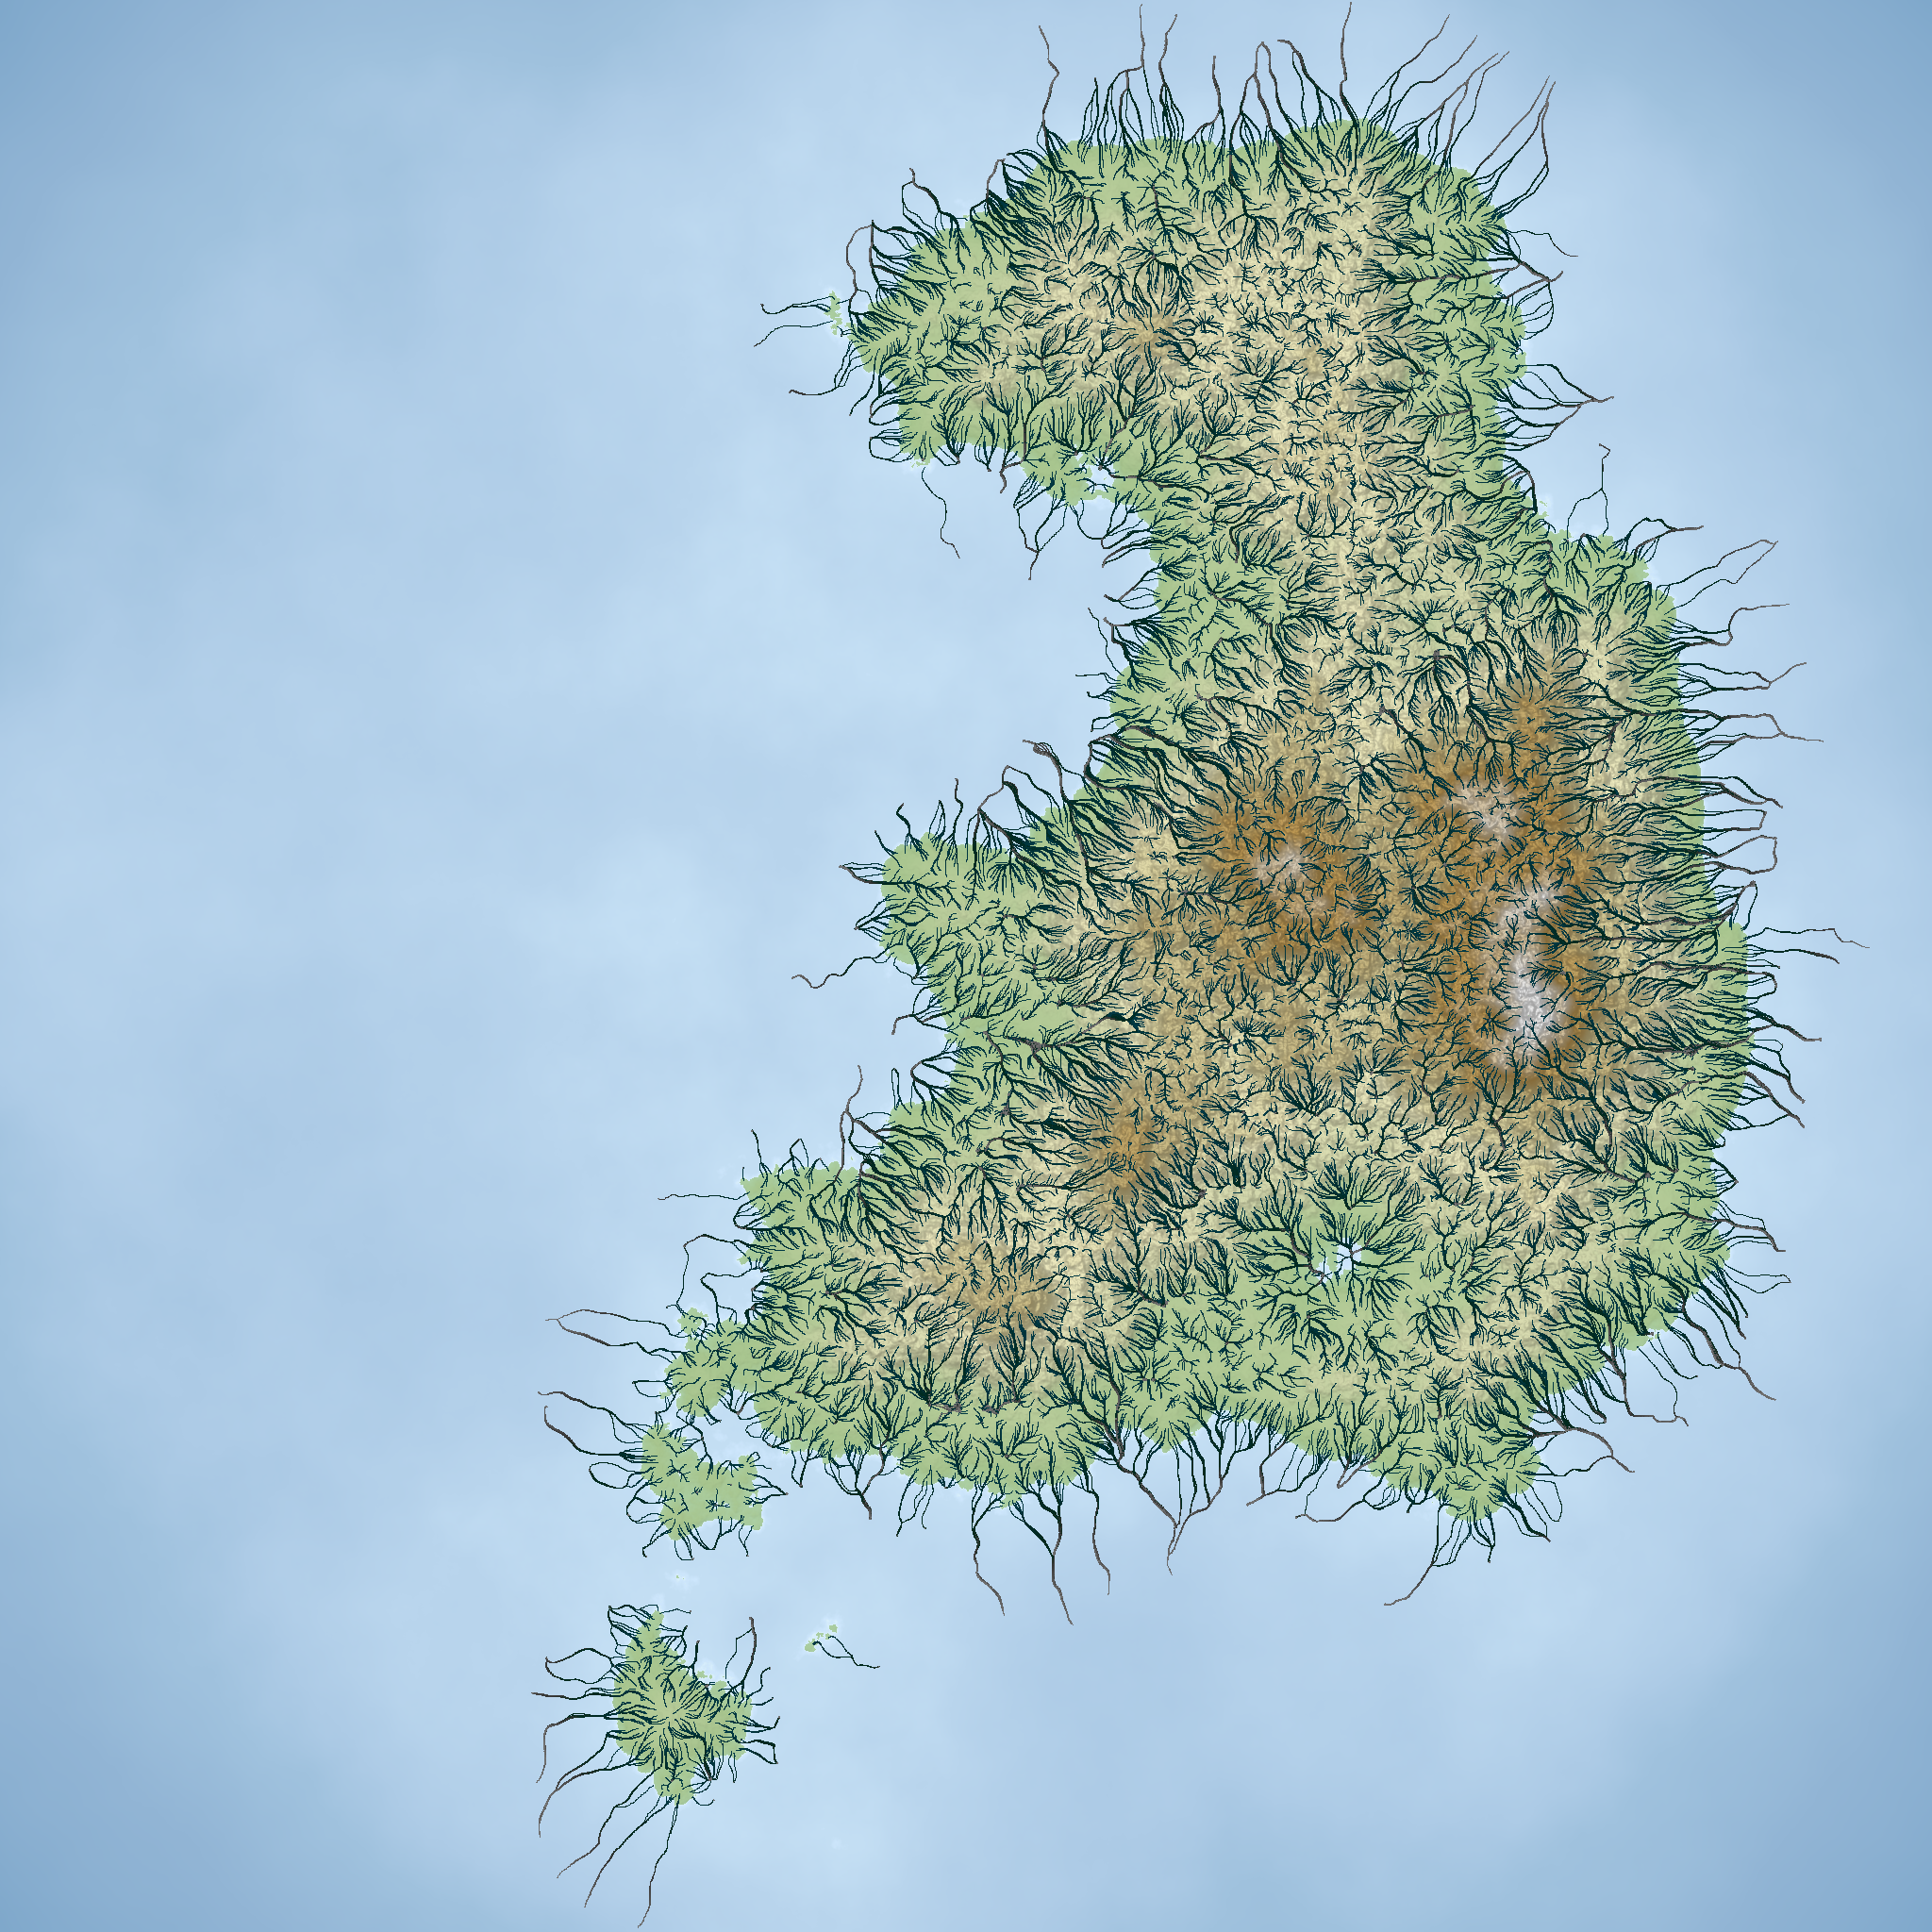
\includegraphics[width=0.45\textwidth]{data/86_rendered_droplets.png}
  \hfill
  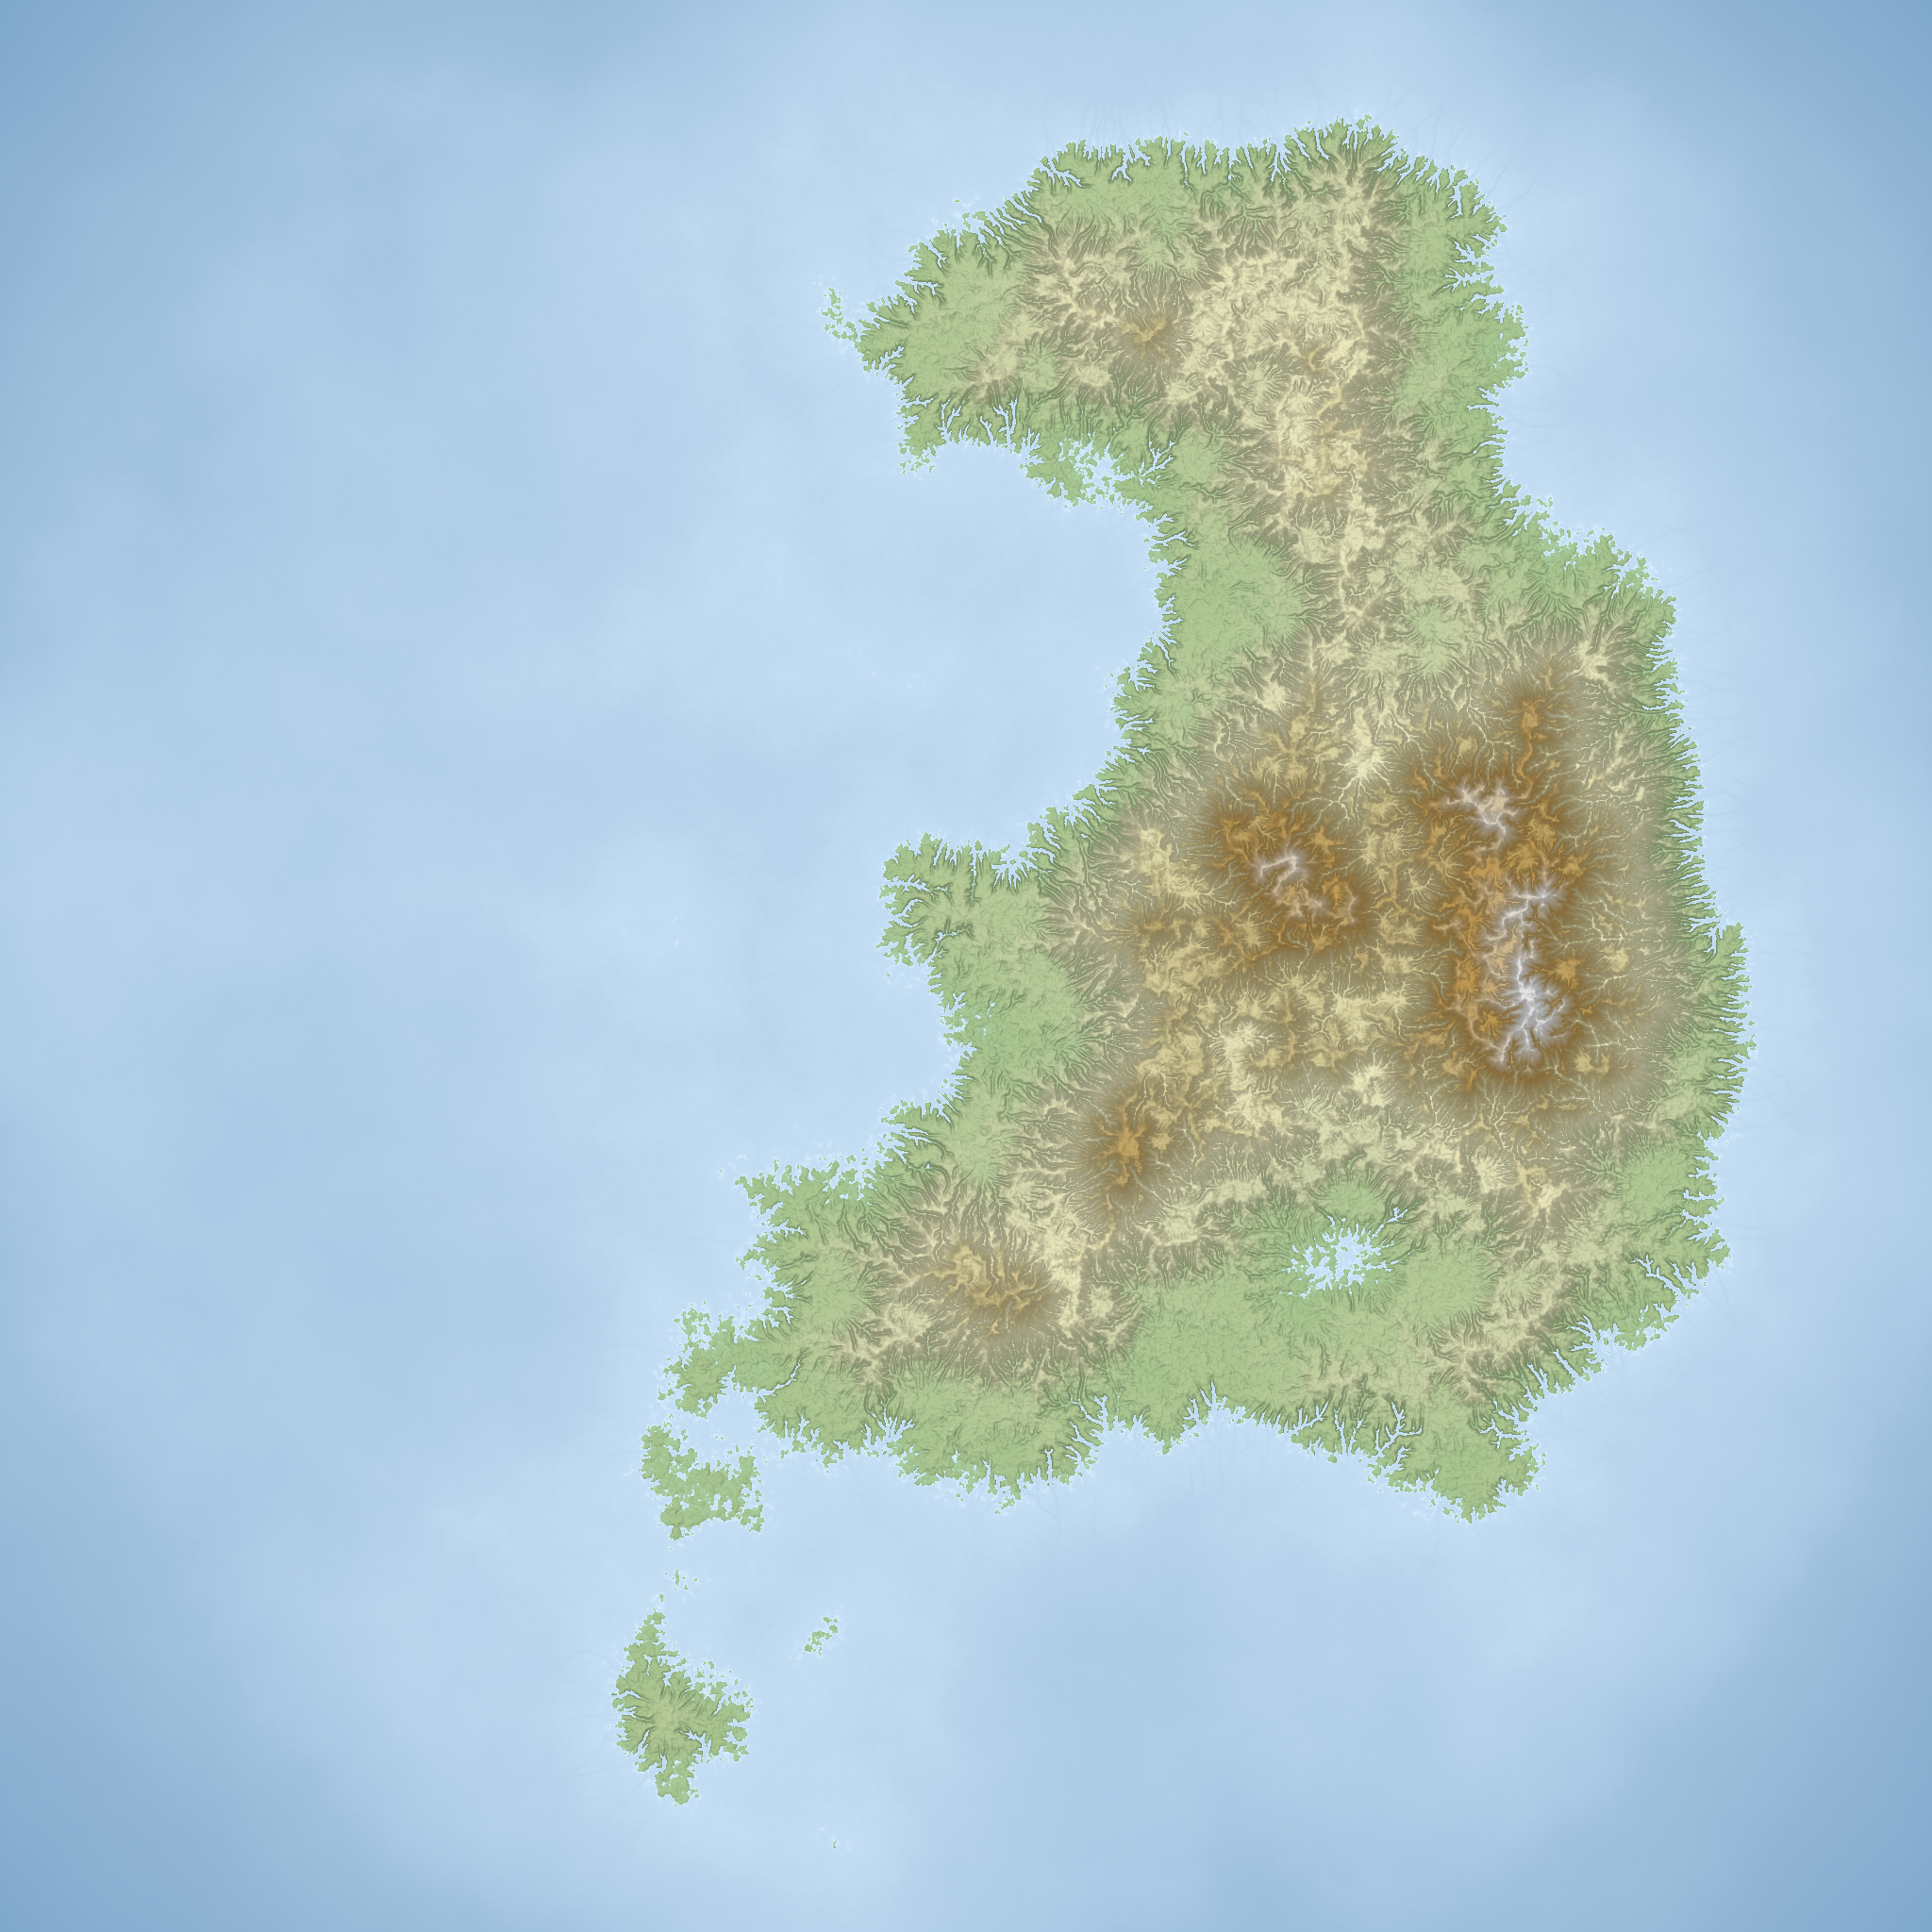
\includegraphics[width=0.45\textwidth]{data/86_rendered.png}
}

\def\ulohaTarget{Dir}
\begin{uloha}
  Daj to celé dokopy a naprogramuj generovanie náhodných ostrovov.
\end{uloha}
\def\ulohaTarget{File}

Tu je niekoľko ďalších ostrovov, ktoré sa vygenerovali s rôznymi seedmi:

\def\tmp#1{
  \centerline{
\foreach\n in {#1}{
  \includegraphics[width=0.33\textwidth]{data/ostrovy/\n_rendered.png}
}}}

\tmp{100,263,264}

\vskip 1ex

\tmp{265,266,267}

\vskip 1ex

\tmp{26,273,53}


Samozrejme, v tomto projekte by sa dalo pokračovať k realistickejším výsledkom, ale chcel
som ti len ukázať, ako sa náhodné čísla dajú použiť na vytváranie vecí, ktoré sú 
''len trochu'' náhodné. 


\chapter{Hešovanie: \vb{<unordered\_set>} a \vb{<unordered\_map>} v STL}
\label{sect:hesovanie}


Vráťme sa k úlohe~\ref{uloha:ziarovky-vela}. Opäť budeme mať žiarovky, ktoré
budú mať výrobné čísla \prg!unsigned long!, takže budú z rozsahu $0$ až $M-1$, 
kde $M=2^{64}$. Zároveň pre jednoduchší začiatok predpokladajme, že vieme, 
že budeme mať presne $n\ll M$ žiaroviek. Na vstupe budú  opäť chodiť príkazy na prepnutie
žiarovky a otázky, či nejaká žiarovka svieti. V kapitole \ref{sect:stromy} sme
to riešili použitím vyhľadávacích stromov. Teraz si ukážeme iný spôsob riešenia,
ktorému sa hovorí {\em hešovanie}.


Keby sme z nejakého dôvodu vedeli, že nám budú v nejakom poradí chodiť žiarovky
s číslami $42$, $43$, $44, \ldots, 41+n$, stačilo by rezervovať si pole \prg!bool A[n]!
a stav žiarovky s číslom $z$ by sme si mohli pamätať v premennej \prg!A[z-42]!. 
Podobne keby sme vedeli, že budú chodiť žiarovky $2,4,\ldots,2n$, tiež by stačilo rezervovať
pole  \prg!bool A[n]! a žiarovku s číslom $z$ by sme mali v premennej \prg!A[z/2-1]!.
V oboch prípadoch by sme mali nejakú funkciu \prg!int h(unsigned long z) { ... }!,
ktorá pre číslo žiarovky vyráta jej umiestnenie v poli, takže žiarovka $z$
je umiestnená v \prg!A[h(z)]!. Ideálne by bolo, keby som mohol mať
jednu takú funkciu \vb{h}, ktorá by fungovala pre viacero (ideálne pre všetky)
možné vstupy. Každú funkciu \vb{h}, bez ohľadu na to, ako sa vypočíta,
si viem predstaviť ako kartičku, kde pre každý z $M$ bodov v hornom riadku (všetky možné výrobné čísla)
ide šípka do nejakého bodu v spodnom riadku (všetky pozície v poli).

\centerline{
  \begin{tikzpicture}
    \tikzstyle{sipkaA}= [teal,->,shorten >= 0.75ex]
    \tikzstyle{sipkaB}= [magenta, very thick,->,shorten >= 0.75ex]
  \def\dot(#1){\filldraw (#1) circle (1.5pt)}
  \def\hi{2}
  \def\M{13}
  \def\n{6}
  \pgfmathsetmacro{\lox}{(\M-\n)/2-1}

  \foreach \t/\s [count=\x] in {1/A,2/A,1/B,3/B,2/B,5/A,6/A,2/A,3/A,4/B,5/A,6/A,5/B,6/B} 
    \draw[sipka\s] (\x-1,\hi) -- (\t+\lox,0);

  \foreach \x in {0,...,\M}
    \dot(\x,\hi);

  \xdef\alist{0,1,2}
  \pgfmathtruncatemacro{\tmp}{\M-4}
  \foreach \i in {0,...,\tmp} {
    \xdef\alist{\alist, {...} }
  }
  \xdef\alist{\alist, M-1}
  \foreach \l [count=\x] in \alist
    \node[above,yshift=1.5ex] at (\x-1,\hi) {{\small$\l$}};
  
  \foreach \x in {1,...,\n}
    \dot(\x+\lox,0);

  \xdef\alist{0,1}
  \pgfmathtruncatemacro{\tmp}{\n-4}
  \foreach \i in {0,...,\tmp} {
    \xdef\alist{\alist, {...} }
  }
  \xdef\alist{\alist, n-1}
  \foreach \l [count=\x] in \alist
    \node[below,yshift=-1.5ex] at (\x+\lox,0) {{\small$\l$}};

\end{tikzpicture}}

Ak používam túto konkrétnu funkciu \vb{h}, tak
pri každom spustení sa na vstupe ocitne $n$ rôznych výrobných čísel (fialové šípky)
a o týchto chceme, aby sa zobrazili na rôzne miesta. Keď sa nad tým chvíľu zamyslíš,
tak je zrejmé, že to nemôže fungovať: nech sú šípky zoradené hocijako,
máme $M$ šípok a $n$ cieľov, preto musí
byť cieľ, do ktorého smeruje aspoň $M/n$ šípok. No a keďže $M$ je veľmi veľké, 
dá sa nájsť vstup, v ktorom všetkých $n$ vybratých
šípok ukazuje do tej istej pozície.

Napriek tomu, že je jasné, že to nebude fungovať, skúsme byť chvíľu tvrdohlaví
a pokračovať v úvahách. Dajme tomu, že by sme mali nejakú takúto {\em hešovaciu} funkciu \vb{h},
\indexItem{Alg}{hešovacia funkcia, kolízie}
teda nejak vybraté modré šípky. Podľa toho, ktoré
výrobné čísla sa objavia na vstupe, niektoré šípky budú fialové.
Nedúfame, že naša funkcia bude úplne dokonalá, a tak sa nám možno môže stať, že niekoľko
fialových šípok bude smerovať do rovnakého cieľa. Ak ich ale nebude veľa, 
ešte to nie je stratené. Takéto tzv. {\em kolízie} môžeme vyriešiť napr. tak,
že v našom poli \prg!A! si nebudeme na pozícii \prg!h(i)!
ukladať \prg!bool! hodnotu, či je žiarovka s číslom  \prg!h(i)! zapnutá, ale
spájaný zoznam zapnutých žiaroviek so všetkými výrobnými číslami $x$,
pre ktoré $\vb{h}(x)=\vb{h}(i)$. Môžme to naprogramovať napr. takto:


\label{pg:lst:hash}
\begin{lstlisting}
using Key = unsigned long;
using HashFunct = function<int(Key)>;
  
struct HashMap { 
  vector<forward_list<Key>> A;
  HashFunct h;
    
  HashMap(int n, HashFunct _h) : h{_h} { A.resize(n); }
  
  void insert(Key x) {
    auto &list = A[h(x)];
    if (find(list.begin(), list.end(), x) == list.end()) 
      list.push_front(x);
  } 
    
  void erase(Key x) {
    auto &list = A[h(x)];
    auto it = find(list.begin(), list.end(), x);
    if (it != list.end()) {
      *it = *list.begin();
      list.pop_front();
    }
  } 
  
  bool contains(Key x) {
    auto &list = A[h(x)];
    return find(list.begin(), list.end(), x) != list.end();
  }
};  
\end{lstlisting}

V tomto programe je hešovacia funkcia typu \prg!HashFunct!, t.j. dostane parameter $x$
a vráti hodnotu $h(x)$ z rozsahu $0,\ldots,n-1$. Premenná typu 
\prg!HashMap! dostane v konštruktore dĺžku poľa $n$ a hešovanciu funkciu, 
a potom má metódy \prg!insert!, \prg!erase! a \prg!contains!, ktoré sú zjavné.
Mohli by sme teda napísať
napr. \prg!HashMap h(10, [](Key x) { return x % 10; });!.
a po tom, čo postupne zavoláme \vb{insert} s hodnotami 
\vb{77 5 23 18 43 57 15 43 42 85 } to bude v pamäti vyzerať takto:\\


\centerline{\begin{tikzpicture}[scale=0.8]
  \def\h{0.35}
  \def\nodecolor{cyan!50!blue}
  \foreach \i in {0,...,9} {
  \draw(\i,0) rectangle (\i+1,2*\h);
  \node[above]at(\i+0.5,2*\h){$\i$};
  \fill[\nodecolor](\i+0.5,\h) coordinate (base\i)circle (0.1); 
  }
  \node[anchor=east]at(0,0.5){\vb{A}:};

  \def\zoz#1(#2,#3)#4{
    \begin{scope}[shift={($(#2,1.15*#3)+(0.5,0.5)$)}]
      \draw[\nodecolor,rounded corners=2pt](-0.4,-\h) rectangle (0.4,\h);
      \node[\nodecolor] at(0,0) {\vb{#4}};
      \coordinate (top#1) at (0,\h);
      \coordinate (bot#1) at (0,-\h);
      \fill[\nodecolor] (bot#1) circle (0.1);
  \end{scope}
  }

  \foreach \x/\l in {2/{4},3/{4,2},5/{8,1,{}},7/{5,7},8/{1}} {
    \foreach \val [count = \i, 
        remember = \c as \lastC (initially base\x)
    ] in \l {
        \zoz{\i}(\x,-\i){\val\x}
        \def\c{bot\i}      
        \draw[\nodecolor, ->] (\lastC) -- (top\i);
    }
  }

\end{tikzpicture}}


Akú by mal náš program zložitosť? Každá z funkcií \vb{insert}, \vb{erase}, \vb{contains}
najprv vyráta hešovaciu funkciu (nateraz predpokladajme, že to vieme urobiť rýchlo)
a potom v najhoršom prípade prehľadá celý spájaný zoznam \prg!A[h(x)]!. Takže zložitosť každej
operácie je úmerná dĺžke zoznamu \prg!A[h(x)]!. V zozname \prg!A[h(x)]! skončia všetky
žiarovky zo vstupu, ktorých výrobné číslo má v našej hešovacej funkcii kolíziu s výrobným
číslom $x$, t.j. žiarovky s číslom $z$, pre ktoré platí $\vb{h}(x)=\vb{h}(z)$,
preto zložitosť nášho programu bude závisieť od počtu kolízii našej hešovacej funkcie.


A sme zase tam, kde sme boli na začiatku: nech si zvolíme hocijakú hešovaciu funkciu,
vždy bude existovať vstup, na ktorom bude mať veľa kolízií. 
Opäť nám ale príde na pomoc náhoda. Na začiatku síce nevieme, aké výrobné čísla
budú na vstupe, ale ako funkciu \prg!h! si vyberieme náhodnú funkciu. Čo to znamená
náhodná funkcia? Funkcia je obrázok, kde z každého z $M$ výrobných čísel ide
modrá šípka do niektorého z $n$ miest. Koľko
je takých rôznych obrázkov? Na obrázku je $M$ šípok a každá z nich má $n$ možných cieľov,
teda dokopy je $n^M$ možností. Napíšeme si ich na papieriky a vložíme do vrecka.
Potom náhodne vytiahneme jeden obrázok a máme náhodnú funkciu.
Kontrolná otázka:

\begin{uloha}
  \label{uloha:nahprm}
  Vyberme si náhodnú funkciu \prg!h!. Aká je pravdepodobnosť, že $\vb{h}(42)=1$?
\end{uloha}

Vyšlo ti $1/n$? Dobre. Jedna možnosť, ako sa o tom presvedčiť, je pozrieť sa na
všetkých $n^M$ papierikov a ofarbiť ich podľa toho, aká je hodnota $\vb{h}(42)$:
ak  $\vb{h}(42)=0$, papierik bude modrý, ak  $\vb{h}(42)=1$, bude červený atď.
Vo vrecku teda budem mať papieriky $n$ farieb. Koľko je tam papierikov jednej farby?
Bez ohľadu na to, kam smeruje šípka $\vb{h}(42)$, ostatné šípky sú umiestené hocijako,
a teda mám $n^{M-1}$ možností. Pôvodnú úlohu sa teraz
viem opýtať takto: vo vrecku mám $n^M$ papierikov ofarbených $n$ farbami, 
pričom z každej farby mám rovnako veľa, t.j. $n^{M-1}$ papierikov.
Aká je pravdepodobnosť, že vytiahnem červený papierik? Tu je ale odpoveď jasná:
červených papierikov je $n^{M-1}$, preto pravdepodobnosť je  $n^{M-1}/n^M=1/n$.


Koľko kolízií so vstupom má náhodná funkcia? To, samozrejme, závisí od toho, aký papierik
si vytiahneme. Môžme mať šťastie a vytiahneme si takú funkciu, čo nebude mať žiadne kolízie, môžeme mať smolu a 
bude ich mať veľa. Toto je v istom zmysle typická situácia, ktorú sme zažili aj pri porovnávaní
súborov: náhoda nám môže pomôcť urobiť veci efektívne, 
ale zaplatíme za to tým, že s malou pravdepodobnosťou nám to nevyjde. Preto aj teraz
nás nebude zaujímať najhorší prípad (ktorý, dúfame, bude nastávať s malou pravdepodobnosťou),
ale {\em očakávaný prípad}.

\section*{Ďalšia odbočka, tentokrát o očakávanej hodnote.}
\label{mat.expectation}

\def\tmp[#1]#2{\textcolor{#1}{\raisebox{-1.20pt}{\usymH{\kocka#2}{2ex}}}}

V časti~\ref{sect:nahoda} sme hovorili o tom, že môžme mať nejaký náhodný proces, napr.
že hodím oranžovou a modrou kockou. Výsledkom je nejaký jav, napr. \tmp[orange]5 \tmp[teal]3,
ktorý má nejakú pravdepodobnosť (v tomto prípade $1/36$). Niečo, čo viem vypočítať z výsledku
takéhoto náhodného procesu, sa v matematike volá {\em náhodná premenná}. V príklade s \indexItem{Mat}{náhodná premenná}
dvoma kockami môžem mať napr. náhodnú premennú $X$, ktorá vyráta, koľko bodiek je na tej kocke,
na ktorej padlo väčšie číslo, takže napr. $X(\tmp[orange]5\;\tmp[teal]3)=5$, 
$X(\tmp[orange]1\;\tmp[teal]4)=4$. Pretože $X$ závisí iba od výsledku nášho náhodného procesu (hodu),
môžme sa napr. pýtať, aká je pravdepodobnosť, že $X=3$ (čo budeme značiť $\pr{X=3}$). 
Možnosti, pri ktorých je na väčšej kocke číslo $3$, sú 
\tmp[orange]1 \tmp[teal]3, \tmp[orange]2 \tmp[teal]3, \tmp[orange]3 \tmp[teal]3,
\tmp[orange]3 \tmp[teal]2 a \tmp[orange]3 \tmp[teal]1, čiže $5$ možností. Všetkých možností je 
$36$, preto $\pr{X=3}=5/36\approx0.14$. 
Všetky pravdepodobnosti si môžeme napísať do tabuľky:\\

% parametre: nazov, makro s parametrami (i,j) co nastavi \res a \clr, zoznam hodnot (od 1)
\def\nahPrem#1#2#3{%
\centerline{
  \begin{tikzpicture}[scale=0.5]
    \node[anchor=south east] at (0,0) {\large$#1$};
  \foreach\i in {1,...,6} {
    \node at (\i-0.5,0.5) {\tmp[teal]{\i}};
    \node at (-0.5,0.5-\i) {\tmp[orange]{\i}};
  }
  \foreach\i in {1,...,6}{
    \foreach \j in {1,...,6} {
      \csname #2\endcsname{\i}{\j}
      \filldraw[draw=none,fill=\clr!10](\i-1,0-\j) rectangle 
      node[align=center]{$\res$}(\i,1-\j);
    }}
  \draw[very thin, gray] (-0.9,0.9) grid (6,-6);
  \draw (-1,0) -- (6,0) (0,1) -- (0,-6);

    \begin{scope}[shift={(12,-3)},scale=1.2]
   \draw (-3,0) -- (0.2,0) (0,1) -- (0,-1);
    \node at (-1.8,0.5){$i$};  
    \node at (-1.8,-0.5){$\pr{#1=i}$};  
      \foreach \p[count=\i] in {#3}{
      \draw[very thin, gray] (\i,0.9) -- (\i,-0.9);
      \draw (\i-0.8,0) -- (\i+0.2,0);
      \node at (\i-0.5,0.5) {$\i$};  
      \node at (\i-0.5,0-0.5) {$\frac{\p}{36}$};  
    }
    \end{scope}
\end{tikzpicture}
}
}

\def\fnX#1#2{%
 \ifnum\i>\j\def\res{\i}\else\def\res{\j}\fi
 \def\clr{\ifcase\res\relax\or yellow\or orange\or red\or magenta\or blue\else green\fi}
}


\nahPrem{X}{fnX}{1,3,5,7,9,11}


Akú hodnotu $X$ môžeme očakávať, keď hodíme dvoma kockami? S najväčšou pravdepodobnosťou to 
bude 6, ale aj 5 a 4 budú dosť časté. Preto nie je rozumné povedať, že očakávame ten výsledok,
ktorý má najväčšiu pravdepodobnosť. Radšej si predstavme, že by som hádzal veľakrát a zrátajme, 
aký bude priemer hodnôt $X$, ktoré dostanem. Z časti~\ref{sect:nahoda} vieme, že ak 
$n$-krát zopakujeme náhodný proces, v ktorom je nejaký jav s pravdepodobnosťou $p$, 
tak náš jav nastane zhruba $pn$-krát\footnote{Keby nastal príliš viackrát alebo príliš menejkrát,
vedeli by sme urobiť prediktor a už by to nebol náhodný proces.}. Preto keď hodíme
$n$-krát kockami,  $\frac{n}{36}$-krát bude hodnota $X$ jedna, $n\frac{3}{36}$-krát dva
a tak ďalej. Priemer zo všetkých hodov preto bude 
$$\frac{1}{n}\left(\frac{n}{36}+2n\frac{3}{36}+3n\frac{5}{36}+4n\frac{7}{36}+5n\frac{9}{36}+
6n\frac{11}{36}\right)=\frac{1}{36}(1+6+15+28+45+66)=161/36\approx4.47.$$\indexItem{Mat}{stredná hodnota}
Očakávaná hodnota\footnote{V angličtine {\em expected value}, v slovenčine sa tomu správne
hovorí {\em stredná hodnota}. Treba si dať pozor, že to nie je hodnota, ktorú najčastejšie dostanem
(napr. na kocke mi ťažko padne číslo $4.47$), ale priemer hodnôt cez veľa pokusov.}
náhodnej premennej $X$ je teda $161/36$, čo sa zvykne zapísať \hbox{$\ev{X}=161/36$.} 


Predchádazjúce počty sa často opakujú, tak si ich poďme zapísať všeobecne. Majme náhodnú premennú
$X$, ktorá má hodnoty prirodzené čísla. Aby som si zjednodušil zápis, budem používať
\pr{X=i} pre hocijaké $i$ s tým, že pre niektoré $i$  je $\pr{X=i}=0$ (napr. v našom prípade pre všetky
$i>6$). 
Po $n$ opakovaniach budem mať výsledok s hodnotou $i$ zhruba $\pr{X=i}$-krát, preto  priemerná hodnota
bude
$$\ev{X}=\frac{1}{n}\left(n\cdot\pr{X=1}+2n\cdot\pr{X=2}+3n\cdot\pr{X=3}+\cdots\right)$$
Číslo $n$ sa pri úpravách stratí, preto výsledok viem elegantne zapísať\footnote{\indexItem{Mat}{zápis sumy}
  Tu som použil matematickú verziu \vb{for} cyklu, ktorá sa značí veľkým gréckym písmenom $\sum$
  ({\em sigma}, čosi ako naše {\em s} v slove {\em suma}). Podobne ako pri \vb{for} cykle, aj v sume
  mám premennú, ktorá postupne nadobúda hodnoty od jedného čísla po druhé. Za znakom $\sum$ môžem
  mať hocijaký výraz s mojou premennou a výsledky sa sčítajú. Napr. $1+2+3+4+5$ by som 
  mohol napísať $\sum\limits_{x=1}^5x$. Podobne $1\cdot2+2\cdot3+3\cdot4+\cdots+n(n+1)$ by som 
  napísal $\sum\limits_{x=1}^nx(x+1)$. Často sa hodí si nejaké premenné očíslovať a potom v sume
  používať index podobne ako v poli. Napr. ak mám čísla $a_1,a_2,\ldots,a_n$, tak ich 
  priemer je $\frac{1}{n}\sum\limits_{i=1}^na_i$. 
}ako 

\begin{equation*}\boxed{\ev{X}=\sum_{i=1}^\infty i\cdot\pr{X=i}}\end{equation*}


Urobme si podobnú náhodnú premennú $Y$, ktorá namiesto väčšieho bude vracať menšie číslo z dvoch
kociek.

\def\fnY#1#2{%
  \ifnum\i<\j\def\res{\i}\else\def\res{\j}\fi
 \def\clr{\ifcase\res\relax\or yellow\or orange\or red\or magenta\or blue\else green\fi}
}


\nahPrem{Y}{fnY}{11,9,7,5,3,1}


Strednú hodnotu vypočítame 
$\ev{Y}=\frac{11}{36}+2\frac{9}{36}+3\frac{7}{36}+4\frac{5}{36}+5\frac{3}{36}+6\frac{1}{36}=
\frac{91}{36}\approx2.53$. To znamená, že ak budeme hádzať dvoma kockami, tak priemerná
hodnota na menšej z nich bude $2.39$. Na rátanie strednej hodnoty sa dá pozrieť 
ešte inak: v tabuľke vľavo sú hodnoty $Y$ pre všetky možné výsledky. Keď rátame 
napr. \pr{Y=2} tak sa pozrieme do tabuľky a spočítame, koľkokrát je výsledok $2$;
v našom prípade dostaneme $\pr{Y=2}=\frac{9}{36}$. Keď rátame strednú hodnotu, tak
číslo $i=2$ násobíme \pr{Y=2}, t.j. máme $2\frac{9}{36}$. To je ale to isté, ako keby sme pre
každé políčko tabuľky, kde je dvojka (takých je $9$) zarátali hodnotu $2\frac{1}{36}$. To 
platí samozrejme nielen pre dvojku, takže môžme napísať

$$\ev{Y}=\frac{1}{36}\cdot\sum_{a=\tmp[orange]1}^{\tmp[orange]6}\;\;\sum_{b=\tmp[teal]1}^{\tmp[teal]6}Y(a,b)$$

Týmto sme vlastne vyrátali priemerné číslo z tabuľky vľavo.
Takže (za predpokladu, že každý výsledok má rovnakú pravdepodobnosť) očakávaná hodnota náhodnej
premennej je priemerná hodnota cez všetky možné výsledky. To dáva zmysel: každý výsledok má rovnakú
pravdepodobnosť, takže ak veľakrát opakujem hod, každý výsledok stretnem rovnaký počet krát.


Náhodné premenné sú funkcie, ktoré z výsledku náhodného procesu rátajú nejaké číslo. Preto
ich môžem napríklad aj sčítať. Takže môžem mať náhodnú premennú $Z=X+Y$, pre ktorú napr.
$Z(\tmp[orange]3\;\tmp[teal]5)=X(\tmp[orange]3\;\tmp[teal]5)+Y(\tmp[orange]3\;\tmp[teal]5)=5+3=8$.
$Z$ je vlastne súčet oboch kociek ($X$ je väčšia a $Y$ menšia), a teda vyzerá takto:\\

\def\fnZ#1#2{%
 \pgfmathtruncatemacro{\res}{#1+#2}
 \def\clr{\ifcase\res\relax\or\relax\or 
 yellow\or orange\or red\or magenta\or blue\or green\or
 yellow\or orange\or red\or magenta\or blue\else green
 \fi}
}


\nahPrem{Z}{fnZ}{0,1,2,3,4,5,6,5,4,3,2,1}

Stredná hodnota je (po troche rátania) $\ev{Z}=\sum\limits_{i=1}^{12}i\cdot\pr{Z=i}=\cdots=7$, 
čo je presne $\ev{X}+\ev{Y}$. Nech by $X$ a $Y$ boli hocijaké, môžem si napísať\indexItem{Mat}{súčet stredných hodnôt}

\begin{align*}
  \ev{Z}&=
\frac{1}{36}\cdot\sum_{a=\tmp[orange]1}^{\tmp[orange]6}\;\;\sum_{b=\tmp[teal]1}^{\tmp[teal]6}Z(a,b)=
\frac{1}{36}\cdot\sum_{a=\tmp[orange]1}^{\tmp[orange]6}\;\;\sum_{b=\tmp[teal]1}^{\tmp[teal]6}
  \left(X(a,b)+Y(a,b)\right)=\\[2ex]
  &=\frac{1}{36}\cdot\sum_{a=\tmp[orange]1}^{\tmp[orange]6}\;\;\sum_{b=\tmp[teal]1}^{\tmp[teal]6}X(a,b)+
\frac{1}{36}\cdot\sum_{a=\tmp[orange]1}^{\tmp[orange]6}\;\;\sum_{b=\tmp[teal]1}^{\tmp[teal]6}Y(a,b)=
\ev{X}+\ev{Y}
\end{align*}

Tu sme to počítali pre hod dvoma kockami, ale asi je jasné, že to rovnako zafunguje pre hocijaké
náhodné premenné. Preto pre hocijaké dve náhodné premenné platí 
\begin{equation*}\boxed{\ev{X+Y}=\ev{X}+\ev{Y}}\end{equation*}
Tento vzťah  je ozaj užitočný\footnote{%
    Ako vraví známy dialóg zo starého filmu {\em Adéla ještě nevečeřela}:\\
    {\em 
    - Jak primitivní....\\
    - Ale jak účinné!
    }
} a často používaný, ako hneď ukážeme.


Koniec odbočky, naspäť k hešovaniu. Zaujímala nás zložitosť operácií \vb{insert}, \vb{erase},
\vb{contains}, ak budeme predpokladať, že máme náhodnú hešovaciu funkciu \vb{h}. Každá 
z tých operácií, ak sa pýta na prvok \vb{x},  musí v najhoršom prípade prehľadať
zoznam \vb{A[h(x)]}, v ktorom sú všetky prvky zo vstupu, ktoré sa zobrazia na rovnaké
miesto ako \vb{x} (t.j. \prg!h(x)==h(i)!). Povedzme, že na vstupe sú žiarovky
$z_1,z_2,\ldots,z_n$. To budú teraz pre nás nejaké fixné čísla a pýtame sa, aký je očakávaný
počet počet žiaroviek  $z_i$, ktoré majú kolíziu s danou žiarovkou 
$x$, ak zoberieme náhodnú hešovaciu
funkciu. Označme si $Z$ náhodnú premennú, ktorá počíta počet kolízií s $x$. 
$Z$ je teda funkcia, ktorá
dostane hešovaciu funkciu a vyráta, koľko žiaroviek spomedzi $z_1,\ldots,z_n$ má 
kolíziu s $x$. A nás zaujíma stredná hodnota
\ev{Z}. Mohli by sme sa ju pokúsiť vyrátať ako v predchádzajúcej odbočke: zrátať priemerný
počet kolízií s $x$ cez všetky hešovacie funkcie. To vyzerá ako riadna divočina, tak to skúsme
spraviť inak. Pre každú žiarovku $z_i$ si spravme náhodnú premennú $Z_i$. Bude to funkcia,
ktorá dostane hešovaciu funkciu a zistí, či konkrétna žiarovka 
$z_i$ má kolíziu s $x$. Ak áno, $Z_i$ vráti jednotku,
inak nulu\footnote{Takýmto náhodným premenným sa zvykne hovoriť {\em indikátorové} alebo\indexItem{Mat}{indikátorové premenné} 
{\em Bernoulliho}.}. Je jasné, že $Z=Z_1+Z_2+\cdots+Z_n$ (resp. napísané kratšie $Z=\sum_{i=1}^nZ_i$).
No a z predchádzajúcej odbočky viem, že $$\ev{Z}=\ev{\sum_{i=1}^nZ_i}=\sum_{i=1}^n\ev{Z_i}.$$
Takže namiesto toho, aby som rátal divokú strednú hodnotu zložitej náhodnej premennej $Z$, 
stačí mi vyrátať stredné hodnoty jednoduchších náhodných premenných $Z_i$ a výsledky sčítať.
Pozriem sa na nejakú $Z_i$. Môže nadobúdať hodnoty $0$ alebo $1$, preto 
$$\ev{Z_i}=0\cdot\pr{Z_i=0}+1\cdot\pr{Z_i=1}=\pr{Z_i=1}.$$
Sú dve možností. Ak $z_i=x$, tak, samozrejme, nech zoberiem
hocijakú hešovaciu funkciu, tak $\vb{h}(z_i)=\vb{h}(x)$. Preto $\pr{Z_i=1}=1$.
Druhá možnosť, ak $z_i\not=x$ je zaujímavejšia. Rovnako, ako sme riešili úlohu~\ref{uloha:nahprm},
sa dá ukázať, že $\pr{Z_i=1}=\frac{1}{n}$. Takže dokopy mám
$$\ev{Z}=\sum_{i=1}^n\ev{Z_i}=\sum_{i=1}^n\pr{Z_i=1}=1+(n-1)\frac{1}{n}<2.$$
Skvelé! Ehm, čo sme to vlastne zrátali? $E[Z]$ je očakávaná dĺžka spájaného zoznamu v mieste \vb{h(z)} pre
nejakú konkrétnu žiarovku \vb{z}. Keby som teda riešil úlohu so žiarovkami 
pomocou triedy \vb{HashMap} zo strany \pageref{pg:lst:hash}, do ktorej by som na začiatku dal
ako parameter náhodnú hešovaciu funkciu, 
na každú operáciu by mi stačilo
v očakávanom prípade
prehľadať najviac dvojprvkový zoznam \vb{A[h(x)]}. To vyzerá viac ako nádejne.


Lenže na druhý pohľad zistím, že náhodnú funkciu urobiť neviem. Totiž aj keby som ju mal, ako 
by som si ju zapamätal? Keď na vstupe príde číslo \vb{x}, musím nejak vedieť zistiť, aká hodnota
mu prislúcha a to je v podstate rovnaká úloha, ako tá, čo riešim so žiarovkami. Našťastie
sa ukáže, že nepotrebujem zvoliť hešovaciu funkciu náhodne spomedzi všetkých funkcií, ale existujú
rôzne sady funkcií, ktoré fungujú rovnako: ak si vyberiem náhodnú funkciu z tej sady, v očakávanom
prípade budem mať málo kolízií. Jednu z nich ti ukážem, nech to nevyzerá, že je v tom nejaká mágia.


\indexItem{Alg}{univerzálne hešovanie}
Predpokladajme teraz, že $n$ aj $M$ sú mocniny dvojky, takže $n=2^b$ a $M=2^m$. Napr. ak 
je výrobné číslo \prg!unsigned long! a $n=1024$, tak $m=64$ a $b=10$. Hešovacia funkcia \vb{h} bude 
popísaná tabuľkou $T$ zloženou z núl a jendotiek, ktorá má $b$ riadkov a $m$ stĺpcov. Ak mám vyrátať hodnotu
$\vb{h}(x)$, napíšen si $x$ v dvojkovej sústave, bude mať $m$ cifier. Predstavím si ich ako 
masku: ak je na nejakom mieste jednotka, vyberiem príslušný stĺpec. Vybrané stĺpce skombinujem
operáciou \vb{XOR}, t.j. na pozícii, kde je párny počet jednotiek, bude nula, a na
pozícii, kde je nepárny počet jednotiek, bude jednotka. Výsledný stĺpec prečítam
ako $b$-bitové číslo v dvojkovej sústave. Pre tabuľku $T$ a číslo $x$ budem 
túto operáciu značiť $T\cdot x$, ako keby to bolo násobenie\footnote{Ono to vlastne aj násobenie je,
ale to tu teraz nemusíme rozoberať.}\phantomsection\label{page:nasobenie-matic}. Pre nasledovnú tabuľku $T$ je $T\cdot26=12$:


\centerline{\begin{tikzpicture}[scale=0.5]
\pgfmathsetseed{42}
  \foreach\x in {1,2,4} 
  \filldraw[draw=none, fill=green!10] (\x,0) rectangle (\x+1,-4);
  \foreach \i in {1,...,4} {
    \foreach \j in {1,...,6} {
      \pgfmathtruncatemacro{\b}{Mod(10000*random(),2)}
      \node at (\j-0.5,0.5-\i) {$\b$};
  }}
  \draw[thin,gray] (0,0) grid (6,-4);
  \node[left] at (0,-2) {$T$};
  
  \begin{scope}[shift={(0,0.4)}]
    \draw[thin, gray] (0,0) grid (6,1);
    \node[left,teal!60!black] at (0,0.5) {$26$};
    \foreach\b[count=\x] in{0,1,1,0,1,0}
    \node[teal!60!black] at (\x-0.5,0.5) {$\b$};
    \foreach\b[count=\x] in{32,16,8,4,2,1}
    \node[above,magenta] at (\x-0.5,1) {{\scriptsize\roboto\b}};
  \end{scope}

  \begin{scope}[shift={(8,0)}]
    \foreach \b [count=\i] in {1,1,0,0} {
      \node[orange!60!black] at (-1,0.5-\i) {$\mapsto$};
      \node[orange!60!black] at (0.5,0.5-\i) {$\b$};
    }
    \draw[thin,gray] (0,0) grid (1,-4);
    \foreach\b[count=\x] in{8,4,2,1}
    \node[right,magenta] at (1,0.5-\x) {{\scriptsize\roboto\b}};
    \node[orange!60!black] at (0.5,-4.5) {$12$};
  \end{scope}
\end{tikzpicture}}


\begin{uloha}
  \label{uloha:hasher}
  Naprogramuj triedu \vb{HashFunc}, ktorá ako parameter v konštruktore dostane číslo $b$
  a seed a vyrobí si náhodnú tabuľku $T$. Potom bude mať \prg!int operator()(unsigned long x)!
  ktorý pre dané \vb{x} vráti $T\cdot x$.
\end{uloha}

Keď sme počítali počet kolízií pri hešovaní s náhodnou funkciu, dostali sme sa to takejto 
situácie: mali sme pevne daný prvok \vb{x} a prvok $z_i\not=\vb{x}$ 
a pýtali sme sa, aká je pravdepodobnosť (ak zoberieme úplne náhodnú hešovaciu funkciu),
že $z_i$ sa zahešuje na rovnakú pozíciu ako \vb{x}. Vyšlo nám, že je to $1/n$ a potom všetko 
dobre dopadlo. Preto si teraz predstavme rovnakú situáciu, iba sa pýtame, aká je pravdepodobnosť,
že $h(z_i)=h(\vb{x})$, ak ako hešovaciu funkciu vybereime náhodnú\footnote{%
  opäť si predstavme, že všetky možné tabuľky nahádžeme do vrecka a jednu si vytiahneme} tabuľku $T$.
Keďže $x\not=z_i$, je nejaká pozícia, kde sa ich bitové zápisy líšia. Dajme tomu,
že $i$-ty bit $x$ je $0$ a $i$-ty bit $z_i$ je $1$. 
To znamená, že ak mám hocijakú tabuľku $T$, tak v $T\cdot x$ sa
$i$-ty stĺpec nevyberie, čiže hodnoty v $i$-tom stĺpci výsledok $T\cdot x$ nijak neovplyvňujú.
Rozdeľme si teraz všetky možné tabuľky $T$ do skupín: v jednej skupine budú všetky tabuľky, ktoré
sa líšía iba v $i$-tom stĺpci a všetko ostatné majú rovnaké. V každej skupine je preto $n=2^b$ 
tabuliek\footnote{toľko je rôznych kombinácií núl a jendotiek v $i$-tom stĺpci}. My sa pýtame, koľko
je tabuliek, pre ktoré $T\cdot x=T\cdot z_i$. V každej skupine je hodnota $T\cdot x$ rovnaká
pre všetky tabuľky z tej skupiny, ale hodnoty $T\cdot y$ sú všetky rôzne. To preto, lebo každá zmena 
jedného bitu v $i$-tom stĺpci $T$ zmení príslušný bit vo výsledku $T\cdot z_i$:


\centerline{\begin{tikzpicture}[scale=0.5]

\def\base#1{
  \foreach\x in {0,2,3} 
  \filldraw[draw=none, fill=green!10] (\x,0) rectangle (\x+1,-3);
  
  \foreach \x/\v/\b in {0/1/{1,0,1}, 1/0/{0,1,1}, 3/1/{1,0,1}} {
    \node[teal!60!black] at (\x+0.5,0.5) {$\v$}; 
    \foreach \j [count = \y] in \b {
      \node at (\x+0.5,0.5-\y) {$\j$};
    }
  }

  \node [teal!60!black] at (2.5,0.5) {$\mathbf 1$};
  \foreach \i in {0,...,2} {
    \pgfmathtruncatemacro{\tmp}{int(Mod(int(#1/int(2^(2-\i))),2))}
    \node at (2.5,-0.5-\i) {$\mathbf \tmp$};
  }

  \draw[thin,gray] (0,0) grid (4,-3);
  \draw[thick] (2,0) rectangle (3,-3);
  
  \begin{scope}[shift={(4.5,0)}]
    \draw[thin,gray] (0,0) grid (1,-3);
    \foreach \x[count=\i] in {0,1,1} {
      \pgfmathtruncatemacro{\tmp}{int(Mod(\x+int(Mod(int(#1/int(2^(3-\i))),2)),2))}
      \node[magenta] at (0.5,0.5-\i) {$\tmp$};
    }
  \end{scope}
}
  \foreach \x in {0,...,3} \foreach \y in {0,1} {
    \begin{scope}[shift={(8*\x,-5*\y)}]
      \pgfmathtruncatemacro{\p}{\x+4*\y}  
    \base\p
    \end{scope}
  }

\end{tikzpicture}}


Takže z každej skupiny je iba jedna tabuľka $T$, pre ktorú $T\cdot z_i = M\cdot x$, a preto náhodná
tabuľka má pravdepodobnosť $1/n$, že spôsobí kolíziu $z_i$ a $x$. Zvyšok výpočtu prejde rovnako
ako pre úplne náhodné funkcie. 


Preto ak spojíš triedu \vb{HashMap} s výsledkom úlohy~\ref{uloha:hasher}, dostaneš
riešenie úlohy so žiarovkami, kde v priemernom prípade každá operácia prezrie iba konštantne
dlhý zoznam. Oprávnene ale môžeš namietať, že na vyrátanie hešovacej funkcie, t.j. na zránie
$T\cdot\vb{x}$ treba zhruba $\log M\cdot\log n$ operácií, takže sme si oproti vyhľadávaciemu
stromu zase až tak nepomohli. To je pravda, ale dajú sa nájsť podobné sady hešovacích funkcií,
ktoré majú rovnaké vlastnosti, ale dajú sa zrátať rýchlejšie. Napríklad 
ak zoberieme nejaké prvočíslo $p>M$ a náhodnú hešovaciu funkciu urobíme takto: 
zvolíme sí náhodné čísla $a,b$ tak, že $1\le a< p$ a $0\le b< p$ a 
$\vb{h}(x)$ bude $((ax+b) \mod p)\mod n$. Veľmi podobnými, len trochu dlhšími, výpočtami sa dá prísť
na to, že aj táto sada hešovacích funkcií funguje, a navyše sa dá aj rýchlo vyrátať. 


Posledná vec, čo chýba k úplnosti, je znalosť $n$. V úlohe so žiarovkami som zámerne povedal, že je 
dopredu známe, koľko rôznych výrobných čísel sa objaví. V iných úlohách to tak nie je. Dá sa
to však vyriešiť podobne ako v prípade triedy \vb{vector}: budem si sledovať, ako veľmi je moja
hešovacia tabuľka zaplnená, a keď sa zaplní priveľa, zväčším ju a všetky prvky v nej zahešujem
nanovo. Tým sa aj zabezpečí, že ak som mal smolu\footnote{Alebo mi niekto zámerne
zostrojil vstup, v ktorom má moja funkcia veľa kolízií, čo je typický pripad, ak napr. progamuješ
algoritmy na šifrovanie} a niektorý zoznam je príliš dlhý, po prehešovaní očakávam, že sa prvky
rozdelia rovnomerne. 


Môže to celé fungovať?  V STL je trieda \prg!unordered_set!, ktorá sa správa skoro rovnako ako\indexItem{Prg}{\vb{unordered\_set}}
náš starý známy \prg!set!, ale namiesto vyhľadávacieho stromu má hešovaciu tabuľku. To spôsobí,
že iterátor nedáva prvky v utriedenom poradí, a je iba jednosmerný. Ale zase prístup do  
\prg!unordered_set! je o dosť rýchlejší:


%\tikzset{external/force remake}
\begin{tikzpicture}
  \def\plota[#1]#2#3{%
    \addplot[#1,mark=*, 
    line join=round, mark size=0.5pt] table [y=#2, x=n]{data/tree_test2.dat};
    \addlegendentry{\vb{#3}}
  }
  \def\plotb[#1]#2{%
    \addplot[#1, line join=round, mark=none, forget plot,
    name path=#2lo] table [y=#2min, x=n]{data/tree_test2.dat};
    \addplot[#1, line join=round, mark=none, forget plot,
    name path=#2hi] table [y=#2max, x=n]{data/tree_test2.dat};
    \addplot[#1,opacity=0.5,forget plot] fill between[of=#2lo and #2hi];
  }
\begin{axis}[
  width=\textwidth, 
  height=8cm,
  xlabel=$n$,
  ylabel=čas ($\mu$s),
  legend cell align={left},
  legend pos = north west,
  %ymax=0.9,
  %  scaled x ticks=false,
  %scaled y ticks=false,
    /pgf/number format/.cd,
        1000 sep={}
]
%  \plotb[cyan!20]{aa}
%  \plotb[orange!20]{set}
%  \plotb[pink!40]{uset}
  \plota[blue!80]{aa}{aatree.h}
  \plota[orange!80]{set}{set<int>}
  \plota[magenta!80]{uset}{unordered\_set<int>}
\end{axis}
\end{tikzpicture}
%\tikzset{external/force remake=false}


Záverečné poučenie z tejto časti je, že ak nepotrebuješ mať prvky utriedené, je spravidla
niekoľkonásobne rýchlejšie použiť \prg!unoredered_set!, resp. obdobnú \prg!unordered_map!.


Ako všetko v STL, aj \prg!unorederd_set! je šablóna, takže môžeš mať napr. 
\prg!unordered_set<string>!. Ako to ale funguje, keď doposiaľ všetko okolo hešovania
sa dialo na celých číslach? V STL je funkcia, ktorá zo stringu vyráta číslo, a to potom
slúži ako kľúč do hešovacej funkcie. Táto funkcia musí byť tiež starostivo vybraná, lebo
každé dva stringy, ktoré v nej budú mať rovnaký kľúč, skončia vždy v rovnakom zozname v hešovacej 
tabuľke, nech by už hešovacia funkcia bola akokoľvek rafinovaná. Takže ak používaš napr.
\prg!unordered_set<string>!, treba si uvedomiť, že každý prístup znamená prejsť daný string
a zrátať jeho kľúč. 


\prg!unordered_set<string>! je v poriadku, ale keď napíšeš napr. 

\vskip 2ex
\vbox{
\begin{lstlisting}
#include <iostream>
#include <string>
#include <unordered_set>
using namespace std;

struct Clovek {
  string meno;
  int vek;
};

int main() { unordered_set<Clovek> ludia; }
\end{lstlisting}
}

kompilátor vypíše dlhý zoznam chýb, kde sa bude asi medzi iným hovoriť niečo ako\\
\vb{call to implicitly-deleted default constructor of 'unordered\_set<Clovek>'}\\
a možno aj 
\vb{use of deleted function ‘std::hash<Clovek>::hash()’}\\
Tým ti chce povedať, že pre triedu \vb{Clovek} mu chýba práve tá funkcia, ktorá z premennej typu
\vb{Clovek} urobí kľúč do hešovacej tabuľky. Aby si mohol \prg!unordered_set<Clovek>! používať,
treba takú funkciu dodať. Ukážem ti ako, ale na to treba povedať, čo je to tzv. {\em špecializácia
šablóny}.


Dajme tomu, že mám takúto šablónu \indexItem{Prg}{špecializácia šablóny}

\vskip 2ex
\begin{lstlisting}
template <typename T>
struct Vec {
  T x;
  void daj() { cout << "mam vec, ale neviem, co s nou" << endl; }
};
\end{lstlisting}

V programe môžem napísať

\begin{lstlisting}
Vec<int> a; 
Vec<string> b; 
a.x = 42;
b.x = "dvaastyridsat";
a.daj();
b.daj();
\end{lstlisting}

Tým hovorím kompilátoru, aby si zo šablóny vyrobil dva (z pohľadu ďalšieho programu
úplne nezávislé) typy \prg!Vec<int>!
a \prg!Vec<string>!, vyrobil príslušné premenné atď, a keď to spustím, dvakrát sa vypíše tá istá veta.
Niekedy sa ale hodí urobiť výnimku a povedať kompilátoru napr. \cmd{''Všetky typy  
\prg!Vec<string>!, \prg!Vec<bool>!, atď. \ rob podľa šablóny, ale typ \prg!Vec<int>! urob
inak''}. Takáto výnimka sa volá špecializácia a viem ju napísať takto:

\vskip 2ex
\begin{lstlisting}
template <typename T>
struct Vec {
  T x;
  void daj() { cout << "mam vec, ale neviem, co s nou" << endl; }
};

template <>
struct Vec<int> {
  int a;
  Vec(int x, int y) { a = x + y; }
  void daj() { cout << "mam int " << a << endl; }
};
\end{lstlisting}

Zátvorky v \prg!template! ostanú prázdne a za meno typu dosadím parameter, ktorý špecializujem. Takto 
vyrobený typ nemá s pôdovným nič spoločmé, môže mať iné premenné aj metódy. Často je ale
rozumné mať (aj) metódy, čo sa volajú rovnako. Teraz by som mohol napísať

\begin{lstlisting}
Vec<int> a(5,6); 
Vec<string> b; 
b.x = "dvaastyridsat";
a.daj();
b.daj();
\end{lstlisting}

a program by vypísal:

\begin{outputBox}
mam int 11
mam vec, ale neviem, co s nou
\end{outputBox}



Niekedy chcem pri špecializácii zmeniť len zopár detailov a 
chcem, aby väčšina vecí ostala rovnaká, ako v šablóne. V tom prípade môžem špecializovať iba 
jednotlivé metódy takto:\indexItem{Prg}{\vb{struct std::hash}}

\begin{lstlisting}
template <>
void Vec<int>::daj() {cout << "mam int " << x << endl; }
\end{lstlisting}

Opäť začínam prázdnym 
\prg!template <>! a potom nasleduje funkcia, ktorú chcem zmeniť. Musím ale povedať, komu
patrí, a to robím dvoma dvojbodkami. V tomto prípade hovorím \cmd{'' Typ \prg!Vec<int>!
urob podľa šablóny, ale jeho metódu \prg!daj()! urob takto.''}


Funkcia, ktorá pre rôzne typy hovorí, ako vyrobiť kľúč do hešovacej funkcie je v STL
urobená cez triedu \prg!hash!. Je to jednoduchá šablóna, ktorá vyzerá zhruba takto

\begin{lstlisting}
template <typename Key>
struct hash {
  unsigned long operator()(const Key &x) const { ... }
};
\end{lstlisting}

To znamená, že premenná \prg!hash<T> h! má operátor \prg!h(x)!, ktorý zoberie premennú typu 
\prg!T! a vráti jej hešovací kľúč. Môžeš si to vyskúšať, 

\vskip 2ex
\begin{lstlisting}
hash<string> h;
cout << h("hrom do toho") << endl;
\end{lstlisting}

vypíše napr. \vb{14868293708368628758}. Funkcie v \prg!unordered_map! a \prg!unordered_set!
používajú príslušný typ \prg!hash! na to, aby vyrobili hešovacie kľúče. Samotná šablóna
\vb{hash} je naprogramovaná tak, aby spôsobila chybu, všetku prácu musia robiť jej 
výnimky-špecializácie. Keď chcem používať \prg!unordered_set<Clovek>!, musím\footnote{%
no nemusím, sú aj iné možnosti, ale o nich tu teraz nehovorím} preto
dodať špecializáciu \prg!hash<Clovek>!. To môžem spraviť napr. takto:

\vbox{
\begin{lstlisting}
template <>
struct std::hash<Clovek> {
  unsigned long operator()(const Clovek& c) const {
    return 42;
  }
};
\end{lstlisting}
}

Toto by malo byť jasné, jediná vec, čo stojí za pozornosť je, že nakoľko \prg!hash! patrí do
 \prg!namespace std!, tak pri špecializácii musím napísať celé
meno \prg!std::hash! aj keď som si na začiatku ''privlastnil'' všetko zo \prg!std! pomocou
\prg!using namespace std;!.


Hešovacia tabuľka v knižnici \prg!<unordered_map>! potrebuje okrem rátania kľúča objekty porovnávať,
preto do triedy \vb{Clovek} treba pridať operátor \prg!==!

\begin{lstlisting}
struct Clovek {
  string meno;
  int vek;
  bool operator==(const Clovek& c) const {
    return meno == c.meno && vek == c.vek;
  }
};
\end{lstlisting}


Teraz sa program, ktorý používa \prg!unordered_set<Clovek>! bude dať skompilovať aj spustiť,
len namiesto hešovacej tabuľky budem mať len spájaný zoznam: všetky premenné dostanú rovnaký kľúč
$42$, a tak sa vždy zahešujú na to isté miesto, kde vznikne dlhý zoznam. 
Ako môžem získať rozumný kľúč? To je celkom na dlhú diskusiu, ale na bežné účely poslúži aj
jednoduchý prístup: ak \prg!string! a \prg!int! už majú dobré špecializácie \prg!hash!, tak 
ja len vrátim ich \vb{XOR}

\begin{lstlisting}
template <>
struct std::hash<Clovek> {
  unsigned long operator()(const Clovek& c) const {
    return hash<string>()(c.meno) ^ hash<int>()(c.vek);
  }
};
\end{lstlisting}

Čo je to za zápis? \prg!hash<string>()! je volanie konštruktora, t.j. vyrobí 
premennú typu \prg!hash<string>!. Vzápätí zavolám jej \prg!operator()(const string &x)!
s parametrom \prg!c.meno! a dostanem nejaké číslo typu \prg!unsigned long!. Dočasnú premennú
typu \prg!hash<string>! potom zahodím. Rovnako sa to urobí pre \prg!hash<int>!. Takže nakoniec
mám dve čísla, z ktorých urobím bitový \vb{XOR} (\prg!^!).


\chapter{Projekt  Breakthrough }
\label{projekt.breakthrough}

\tikzset{pgfornamentstyle/.style={line width=0.05pt}}
\def\wP#1#2{
    \filldraw[fill=white,draw=black] (#1,#2) circle (0.4);
    \node[very thin] at (#1,#2) {\pgfornament[width = 0.46cm,color = black]{12}};
}
\def\wPn#1#2#3{
  \wP#1#2
  \node[circle, fill=white, inner sep = 0.5pt] at (#1,#2) {#3};
}
\def\bP#1#2{
    \filldraw[fill=black,draw=black] (#1,#2) circle (0.4);
    \node[very thin] at (#1,#2) {\pgfornament[width = 0.46cm,color = white]{4}};
}
\def\bPn#1#2#3{
  \bP#1#2
  \node[circle, fill=black, color=white, inner sep = 0.5pt] at (#1,#2) {#3};
}
\def\boardBg{
  \fill[fill=teal!10!white] (-0.5,-0.5) rectangle (7.5,7.5);
}
\def\boardGrid{
  \draw[shift={(-0.5,-0.5)}] (0,0) grid (8,8);
  \foreach\c[count=\i] in {a,b,c,d,e,f,g,h} \node[below = 0.4] at (\i-1,0) {\c\strut};
  \foreach\i in {1,2,...,8} \node at (-0.9,\i-1) {\i};
}
\def\wPs#1{
    \foreach \x in {#1} {      
      \expandafter\wP\x
    }
}
\def\bPs#1{
    \foreach \x in {#1} {      
      \expandafter\bP\x
    }
}
\def\wC#1{\raisebox{-0.4ex}{\LARGE\libcirc{#1}}}
\def\bC#1{{\LARGE\libcircblk{#1}}}


V nasledujúcich častiach ti ukážem niekoľko ďalších vecí v C++, ktoré je ale najlepšie
vidieť na trochu väčších programoch. Začneme preto s projektom, ktorý nás bude sprevádzať 
dlhší čas: našim cieľom bude napísať program, ktorý hrá hru \btr\footnote{Pravidlá som prevzal z 
\href[pdfnewwindow=true]{https://trmph.com/bin/Basic_Introduction_to_Breakthrough.pdf}{\nolinkurl{https://trmph.com/bin/Basic_Introduction_to_Breakthrough.pdf}}}.
Hru \btr vymyslel r. 2000 Dan Troyka. Jej výhodou je, že má veľmi jednoduché pravidlá
(v porovnaní napr. so šachom),
takže sa ľahko programuje, ale zároveň vôbec nie je jednoduchá na hranie. 
Hrá sa na šachovnici $8 \times 8$. Hrajú dvaja hráči (biely a čierny) a na začiatku
má každý hráč 16 kameňov umiestnených takto:\\
\label{pg:breaktru:def}


\centerline{
%\tikzset{external/force remake}
\begin{tikzpicture}[scale=0.65]
  \boardBg
  \boardGrid
  \wPs{00,10,20,30,40,50,60,70,01,11,21,31,41,51,61,71}
  \bPs{07,17,27,37,47,57,67,77,06,16,26,36,46,56,66,76}
\end{tikzpicture}
}

Hráči sa striedajú na ťahoch (začína biely), pričom v každom ťahu si hráč
vyberie nejaký svoj kameň a pohne ním. Cieľom je dostať niektorý svoj kameň na opačný
koniec šachovnice. Komu sa to podarí prvému, vyhrá (ak hráč príde o všetky
svoje kamene, automaticky prehral). Hráč môže pohnúť svoj kameň o jedno políčko
rovno alebo šikmo, ak je cieľové políčko voľné. Navyše, ak je na cieľovom
políčku súperov kameň, hráč ho môže vyhodiť, ale iba šikmo (ako pešiak v
šachu).




\begin{minipage}[t]{0.5\textwidth}\vspace*{0cm}
\centerline{
%\tikzset{external/force remake}
\begin{tikzpicture}[scale=0.65]
  \boardBg
  \boardGrid
  \bPs{56,76}
  \bPs{52,62}
  \foreach \y in {5,6,7} 
  \draw[blue,thick,->](6,5)--(\y,6);

  \foreach \y in {0,1,2} 
  \draw[blue,thick,->](1,5)--(\y,6);
  
  \draw[blue,thick,->](1,1)--(0,2);
  
  \draw[blue,thick,->](6,1)--(5,2);
  \draw[blue,thick,->](6,1)--(7,2);
  
  \wPn151
  \wPn112
  \wPs{12,22}
  \wPn653
  \wPn614

\end{tikzpicture}
}
\end{minipage}
\begin{minipage}[t]{0.5\textwidth}\vspace*{0cm}
Príklad pravidiel: biely kameň \wC1 môže ísť z b6 na a7, b7, alebo c7, lebo všetky sú voľné.
Biely kameň \wC2 z b2 môže ísť iba na a3, lebo b3 a c3 sú blokované.
Biely kameň \wC3 z g6 môže ísť na f7, g7, alebo h7, pričom ak pôjde na f7 alebo h7
tak zoberie súperov kameň. Napokon kameň \wC4 z g2 môže buď zobrať súpera na f3, alebo prejsť
na h3, ale nemôže ísť na g3.
\end{minipage}





\chapter{Ako udržať poriadok vo veľkých projektoch}
\label{sect:makefile}

V tejto časti budem hovoriť o usporiadaní väčšieho projektu.
Prostredia ako
\link{https://www.codeblocks.org/}{Code::Blocks}, či \link{https://visualstudio.microsoft.com}{MS Visual Studio}
majú spravidla možnosť vytvoriť projekt, ktorý sa skladá z viacerých súborov. 
Ja tu budem ukazovať príklady v prostredí linuxového terminálu: jednak dávajú väčšiu flexibilitu, nie sú závislé od konkrétneho 
prostredia a dá sa na nich najlepšie pochopiť, ako veci interne fungujú.
Pre Windows sa dá nainštalovať napr. \link{https://www.msys2.org/}{MSYS2}, ktorý poskytuje
viac-menej rovnaké prostredie (terminál, príkazy, \ldots). 


Čím väčší program píšeš (a niektoré programy môžu byť veľmi veľké), 
začína byť čoraz dôležitejšie udržovať si v programe
poriadok. Ak dopredu vieš, že program, ktorý ideš písať, môže byť časom dlhší, je 
dobré si v ňom začať dodržovať poriadok už hneď od začiatku. V kapitole
\ref{sect:zasobnik} sme hovorili o tom, že časti programu, ktoré spolu súvisia (napr. 
definíciu triedy a jej metód) je dobré dať do samostatného súboru a do hlavného programu
ho pridať pomocou direktívy \prg!#include!. 
Dobré je aj dať si na začiatok takého súboru
dlhší komentár, kde si napíšeš názvy metód, čo robia ako ako sa používajú: keď budeš po čase potrebovať
zistiť, ako sa tá trieda vlastne používa, nebudeš musieť hľadať hlboko v programe.

Toto ale nerieši iný problém, a tým je čas kompilácie. 
Isto si si všimol, že hlavne ak použiješ optimalizáciu (napr. prepínač \vb{-O3}), program sa
kompiluje pomerne dlho. Ak máš aj program rozdelený do viacerých súborov, preprocesor ich pred
začiatkom kompilácie zlepí do jedného, takže sa vždy kompiluje všetko. Aby sme si ukázali,
ako sa to dá zrýchliť, treba vedieť, že kompilátor vyrába program v dvoch fázach: najprv vyrobí\indexItem{Prg}{object code, linker}
tzv. {\em object code}, kde sú pre všetky funkcie 
vyrobené príkazy pre procesor, ale ešte nemajú presne
určené adresy v pamäti. Object code potom spracuje tzv. {\em linker}, ktorý zoberie kusy z object code
a zlepí ich do výsledného spustiteľného súboru. To, čo trvá dlho, je vyrobiť object code, následné 
linkovanie je krátke. Za normálnych okolností object code ani nevidíš, ale kompilátoru sa dá
(pre \vb{g++} je to prepínač \vb{-c}) povedať, aby ho napísal do súboru a nelinkoval. 
Dajme tomu, že v súbore \vb{main.cc} máš nasledovný program:

\vskip 2ex
\begin{lstlisting}
int cibulka = 4;
int lopata = 5;

int tulipany() {
  int res = 1;
  while (cibulka-- > 0) res <<= 1;
  return res;
}

int jama(int x) { return x * lopata; }

int main() { int x = jama(tulipany()); }
\end{lstlisting}

Kvôli jednoduchosti v ňom nepoužívam \prg!cout!, takže po spustení len do premennej \prg!x!
priradí\footnote{Funkcia \prg!tulipany! nastaví premennú \prg!cibulka! na nulu a pritom ráta hodnotu 
$2^\text{\vb{cibulka}}$. 
Keďže \prg!cibulka!
je na začiatku $4$, tak \prg!tulipany! vráti $16$, čo následne \prg!jama! vynásobí piatimi.} 
$80$ a skončí.
Keď v termináli napíšeš \vb{g++ main.cc -o main} kompilátor vyrobí súbor \vb{main},
ktorý môžeš spustiť \vb{./main} (a nič sa nestane). Ak ale napíšeš \vb{g++ -c main.cc -o main.o} kompilátor vyrobí súbor \vb{main.o}, ktorý obsahuje object code a spustiť nedá.  
Potom môžeš napísať \vb{g++ main.o -o main} a object code z \vb{main.o} sa zlinkuje do súboru
\vb{main}, ktorý sa už spustiť dá. Na súbor \vb{main.o} sa dá pozrieť napr. príkazom
\vb{objdump -Ct main.o}, ktorý vypíše napr. niečo takéto:

\vbox{
\begin{Verbatim}[frame=single]
main.o:     file format elf64-x86-64

SYMBOL TABLE:
0000000000000000 l    df *ABS*	0000000000000000 main.cc
0000000000000000 l    d  .text	0000000000000000 .text
0000000000000000 g     O .data	0000000000000004 cibulka
0000000000000004 g     O .data	0000000000000004 lopata
0000000000000000 g     F .text	000000000000002d tulipany()
000000000000002d g     F .text	0000000000000013 jama(int)
0000000000000040 g     F .text	000000000000001e main
\end{Verbatim}
}

Bez toho, aby sme to rozoberali do detailov vidno, že súbor má dva segmenty:
\vb{.data} a \vb{.text} a v nich obsahuje všetky globálne premenné a
skompilované funkcie uložené za sebou (číslo v prvom stĺpci je adresa). Náš
nápad na zrýchlenie kompilácie by preto bol rozdeliť program do viacerých
súborov, každý z nich prekompilovať do object code a zlinkovať dokopy. Keď sa
potom niečo zmení, bude stačiť prekompilovať ten zmenený súbor a zlinkovať
dokopy s ostatnými, nezmenenými, object súbormi (linkovanie je rýchle).


Spravme si preto súbor \vb{tulipany.cc}, v ktorom bude:

\begin{lstlisting}
int cibulka = 4;

int tulipany() {
  int res = 1;
  while (cibulka-- > 0) res <<= 1;
  return res;
}
\end{lstlisting}

a súbor \vb{jama.cc}, v ktorom bude

\begin{lstlisting}
int lopata = 5;

int jama(int x) {
  return x * lopata;
}
\end{lstlisting}

Teraz môžem napísať \vb{g++ -c tulipany.cc -o tulipany.o} a vyrobí sa súbor \vb{tulipany.o}, ktorý si viem skontrolovať
\vb{objdump -Ct tulipany.o} :

\begin{Verbatim}[frame=single]
tulipany.o:     file format elf64-x86-64

SYMBOL TABLE:
0000000000000000 l    df *ABS*	0000000000000000 tulipany.cc
0000000000000000 l    d  .text	0000000000000000 .text
0000000000000000 g     O .data	0000000000000004 cibulka
0000000000000000 g     F .text	000000000000002d tulipany()
\end{Verbatim}

Rovnako to viem urobiť aj so súborom \vb{jama.cc}. V súbore \vb{main.cc} ale nechcem dávať \prg!#include "tulipany.cc"!, 
to by som bol tam, kde na začiatku, takže mi v ňom ostane

\begin{lstlisting}
int main() { 
  int x = jama(tulipany()); 
}
\end{lstlisting}

Keď teraz ale napíšem \vb{g++ -c main.cc -o main.o}, kompilátor nevyrobí \vb{main.o}, ale začne sa, celkom oprávnene, sťažovať, že jamu ani tulipány nepozná. Toto by bol inak dosť neprekonateľný problém, našťastie C++ má mechanizmus 
tzv. {\em deklarácií}. Čo to je? Ak napíšeš súbor \vb{slon.cc}\indexItem{Prg}{definícia vs. deklarácia}

\begin{lstlisting} 
int slon(int x) {
  return x * 5;
}

int main() {
  int z = slon(3);
}
\end{lstlisting}

je v ňom {\em definícia} funkcie \prg!slon!. Do programu ale môžeš napísať hlavičku funkcie bez tela 
(s bodkočiarkou na konci), čím hovoríš kompilátoru
\cmd{Časom ti definujem takúto funkciu. Ak ju niekde treba použiť, buď v pohode, je to pod kontrolou.} 
Tomuto sľubu sa hovorí {\em deklarácia}.
Samozrejme,
sľub treba dodržať a funkciu časom definovať, ale to sa prejaví až pri linkovaní. Zoberme súbor
\vb{slon.cc}

\begin{lstlisting}
int slon(int x);

int main() {
  int z = slon(3);
}
\end{lstlisting}

Ak napíšem \vb{g++ -c slon.cc -o slon.o}, kompilátor vyrobí súbor \vb{slon.o}, v ktorom je 

\begin{Verbatim}[frame=single]
slon.o:     file format elf64-x86-64

SYMBOL TABLE:
0000000000000000 l    df *ABS*	0000000000000000 slon.cc
0000000000000000 l    d  .text	0000000000000000 .text
0000000000000000 g     F .text	000000000000001c main
0000000000000000         *UND*	0000000000000000 slon(int)
\end{Verbatim}

Všimni si \vb{*UND*} pri symbole \vb{slon(int)}: kompilátor ti uveril, že \vb{slon} nakoniec niekde bude, a do object code
si zaznačil, že zatiaľ ho nenašiel, ale nerobí kvôli tomu paniku. Keby si chcel súbor (aj) zlinkovať (napr.
\vb{g++ slon.o -o slon}), vypíše sa chyba:

\begin{Verbatim}
/usr/bin/ld: /tmp/cc4uVwt3.o: in function `main':
slon.cc:(.text+0xe): undefined reference to `slon(int)'
collect2: error: ld returned 1 exit status
\end{Verbatim}

Teraz linker hovorí, že chcel zlepiť dokopy výsledný súbor, ale slona v žiadnom vstupnom súbore nenašiel. Definíciu
slona môžeš dodať kamkoľvek, napr. ak spravíš súbor \vb{slon.cc} takto:

\begin{lstlisting}
int slon(int x); // ok, deklarácia
int slon(int x); // druhá deklarácia, nie je problém ak je rovnaká

int main() {
  int z = slon(3);
}

int slon(int x) { // definícia
  return x * 2;
}
\end{lstlisting}

Všetko bude v poriadku. Záver z tohoto pozorovania je teda takýto: 

\vskip 2ex 

\centerline{\fcolorbox{magenta}{magenta!3!white}{\parbox{0.9\textwidth}{
\begin{enumerate}\itemsep=-1mm
    \item funkcia môže mať veľa deklarácií (musia byť rovnaké)
    \item funkcia musí mať práve jednu definíciu (inak sa vyrobí object code, ale nezlinkuje sa)
    \item použitiu funkcie v programe musí predchádzať definícia alebo deklarácia
\end{enumerate}
}}}


Naspäť k príkladu s jamou a tulipánom (zmaž všetky súbory \vb{.o}). 
Máme súbory \vb{jama.cc}, \vb{tulipany.cc} a \vb{main.cc}.
Ten zmeníme tak, že pridáme deklarácie príslušných funkcií:

\begin{lstlisting}
int jama(int);
int tulipany();

int main() {
  int x = jama(tulipany());
}
\end{lstlisting}

Teraz treba napísať príkazy:

\begin{Verbatim}[frame=single]
g++ -c jama.cc -o jama.o
g++ -c tulipany.cc -o tulipany.o
g++ -c main.cc -o main.o
g++ main.o jama.o tulipany.o -o main
\end{Verbatim}

a všetko prejde, ako má. Čo ak by som ale chcel v hlavnom programe modifikovať premennú \vb{lopata} (ktorá je v súbore
\vb{jama.cc})? Nemôžem napísať:

\begin{lstlisting}
int jama(int);
int tulipany();

int main() {
  lopata = 10;
  int x = jama(tulipany());
}
\end{lstlisting}

lebo pri kompilovaní \vb{main.cc} a vyhlási chyba, že nepozná premennú \vb{lopata}. Nemôžem napísať ani

\begin{lstlisting}
int jama(int);
int tulipany();

int lopata;

int main() {
  lopata = 10;
  int x = jama(tulipany());
}
\end{lstlisting}

Tým totiž vyrobím (inú) premennú \vb{lopata} v súbore \vb{main.o}. 
Súbor \vb{main.cc} sa skompiluje, ale linker sa bude sťažovať na \vb{multiple definition of `lopata'; }.\indexItem{Prg}{\vb{extern}}
Analógiou deklarácie funkcie je slovíčko \prg!extern! pre premennú: hovorí kompilátoru aby pre ňu nerobil
novú adresu, ale spoľahol sa na to, že časom taká premenná bude definovaná. Výsledný súbor \vb{main.cc}
by teda mohol vyzerať
takto:

\vbox{
\begin{lstlisting}
// odkazy na súbor jama.cc
extern int lopata;
int jama(int);

// odkazy na súbor tulipany.cc
extern int cibulka;
int tulipany();

// hlavný program
int main() {
  lopata = 10;
  cibulka = 7;
  int x = jama(tulipany());
}
\end{lstlisting}
}

Aby sa udržal poriadok, je zvykom deklarácie z nejakého súboru (napr. \vb{jama.cc}) dať do rovnako sa volajúceho 
súboru s príponou \vb{.h} ako {\em header} (napr. \vb{jama.h}) a ten potom vložiť pomocou \prg!#include! všade, kde ho je treba.
Takže do súboru \vb{jama.h} napíšem

\vskip 2ex
\vbox{\begin{lstlisting}
extern int lopata;
int jama(int);
\end{lstlisting}}
do súboru \vb{tulipany.h} napíšem

\vskip 2ex
\vbox{\begin{lstlisting}
extern int cibulka;
int tulipany();
\end{lstlisting}}
a výsledný program bude

\vskip 2ex
\vbox{\begin{lstlisting}
#include "jama.h"
#include "tulipany.h"

int main() {
  lopata = 10;
  cibulka = 7;
  int x = jama(tulipany());
}
\end{lstlisting}}


Metódy tried sú funkcie ako každé iné, a preto pre ne platia rovnaké pravidlá o
deklaráciách a definíciách, ako pre normálne funkcie. Treba len myslieť na to,
že ak sa na metódu odvolávame mimo definície jej triedy, treba ju volať jej
celým menom, t.j. pred menom metódy treba vždy uviesť (s dvomi dvojbodkami)
triedu, ktorej patrí. Porovnaj si tieto dva zápisy

\begin{column}{0.45}
\begin{lstlisting}
struct Bod {
  int x, y;
  int sucet() { return x + y; }
};
\end{lstlisting}
\end{column}
\hfill
\begin{column}{0.45}
\begin{lstlisting}
struct Bod {
  int x, y;
  int sucet();
};

int Bod::sucet() { return x + y; }
\end{lstlisting}
\end{column}

Doteraz sme všetky metódy tried písali tak, ako na príklade vľavo. Oba zápisy robia to isté, ale
je tam drobný rozdiel, ktorý som ti doteraz nespomenul: 
zápis vľavo považuje metódu \vb{sucet} za tzv. {\em inline}: kompilátor ju \indexItem{Prg}{inline metóda}
neskompikuje priamo, ale vždy, keď sa v programe vyskytne jej volanie, kompilátor ho nahradí
programom z definície\footnote{%
  v niektorých prípadoch je to rýchlejšie, ale rastie veľkosť skompilovaného programu}.
Preto zápis vľavo môže byť v header súbore, ale zápis vpravo musíme riešiť rovnako,
ako pri ostatných funkciách.

Zvykom je v definícii typu (triedy) napísať inline iba krátke malé metódy,
pri ktorých nevadí, že sa v skompilovanom programe objavia veľakrát.
Pri ostatných metódach napísať v headri iba ich deklarácie a ich definície písať neskôr. 


Skúsme si to ukázať na trochu zložitejšom príklade.  Vyrob si tri súbory. Prvý bude \vb{vec.h} a bude v ňom

\begin{lstlisting}
#ifndef __vec_h__
#define __vec_h__
struct Vec {
  struct Proxy {          // tento typ sa celým menom volá Vec::Proxy
    Proxy(Vec *a);        // konštruktor Vec::Proxy (deklarácia)
    Proxy &operator++();  // zvýši hodnotu x a vráti referenciu na seba (deklarácia)
    private:
    int *x;               // x je privátne pre Vec::Proxy
  };
  Vec(int x);          // konštruktor Vec (deklarácia)
  int &operator()();   // vráti referenciu na mojaVec (deklarácia)
  Proxy vyrobProxy();  // vyrobí Vec::Proxy, ktorého x ukazuje na mojaVec (deklarácia)
  private:
  int mojaVec;         // privátna hodnota pre Vec
};
#endif
\end{lstlisting}

Je v ňom definovaný typ \vb{Vec}, ktorý má privátnu premennú \vb{mojaVec}, má konštruktor s parametrom \prg!int!,
\prg!operator()()! (t.j. operátor \vb{()} bez parametrov) a metódu \vb{vyrobProxy}. Všetky tri sú iba deklarované,
definície budú v inom súbore. Okrem toho má typ \vb{Vec} svoj vlastný typ \vb{Proxy} (podobne ako iterátory v STL),
ktorý sa celým menom volá \vb{Vec::Proxy}. Ten má svoj vlastný konštruktor a (prefixový) operátor \vb{++}. Tieto
sú tiež v súbore \vb{vec.h} iba deklarované a bude treba ich definovať. Definície budú v súbore \vb{vec.cc}:

\vskip 2ex
\begin{lstlisting}
#include "vec.h" // include treba, aby kompilátor vedel o typoch Vec a Proxy
                 // keď vyrába object code pre vec.cc
Vec::Proxy::Proxy(Vec *a) { x = &a->mojaVec; } // konštruktor pre Vec::Proxy
                                               // x je pointer na a-čkovu mojaVec
Vec::Vec(int x) { mojaVec = x; } // konštruktor pre Vec
int &Vec::operator()() { return mojaVec; }

// zavolaj konštruktor Proxy a daj mu ako parameter pointer na seba
Vec::Proxy Vec::vyrobProxy() { return Proxy(this); }

Vec::Proxy &Vec::Proxy::operator++() {
  (*x)++;
  return *this;
}
\end{lstlisting}

Zápis \vb{Vec::Proxy::Proxy(Vec *a)} treba chápať takto: \vb{Vec} je typ, v ňom je typ \vb{Vec::Proxy}. Hocijaká funkcia \vb{fun}, ktorá
by patrila typu \vb{Vec::Proxy} sa preto celým menom volá \vb{Vec::Proxy::fun}. Konštruktor je metóda, ktorá sa volá rovnako, ako typ
(v našom prípade \vb{Proxy}). Preto celé meno konštruktora je \vb{Vec::Proxy::Proxy}.
A napokon hlavný súbor \vb{main.cc}:

\begin{lstlisting}
#include "vec.h"
#include <iostream>
using namespace std;
int main() {
  Vec v(42);                // konštruktor spraví Vec v, kde v.mojaVec bude 42
  cout << v() << endl;      // v() vráti referenciu na v.mojaVec, vypíše sa 42
  v() += 5;                 // v() je referencia, takže viem v.mojaVec meniť, 
                            // aj keď mojaVec je private
  cout << v() << endl;      // vypíše sa 47
  auto p = v.vyrobProxy();  // p je Vec::Proxy, jeho x je pointer na v.mojaVec
  ++++p;                    //++p inkrementuje v.mojaVec a vráti referenciu na seba
                            // preto ++++p je ++(++p)
  cout << v() << endl;      // vypíše sa 49
}
\end{lstlisting}

Teraz môžeš napísať

\begin{Verbatim}[frame=single]
g++ -c vec.cc -o vec.o
g++ main.cc vec.o -o main
\end{Verbatim}

a po spustení \vb{./main} by sa mali vypísať čísla $42, 47$ a $49$ (všimni si, že pri jednom volaní kompilátora môžem 
zadať viacero vstupných súborov, ktoré môžu byť zmes programov a object code súborov).


Máme hotový mechanizmus, ako udržovať v programe poriadok a zároveň obmedziť čas kompilácie: časti programu, ktoré
logicky patria k sebe (napr. niekoľko tried, ktoré robia jadnu vec a je šanca, že ich použijeme aj inokedy), dáme 
dokopy: typy a deklarácie idú do súboru \vb{.h} a príslušné definície do súboru \vb{.cc}. Súbor \vb{.cc} skompilujeme
do object code, súbor \vb{.h} vložíme pomocou \prg!#include! kam treba. Ak sa niečo zmení, prekompilujeme iba príslušnú časť
a všetko zlinkujeme dokopy. Jediná nepraktická vec je, že na vyrobenie programu musíme veľakrát spúšťať kompilátor s rôznymi parametrami,
a musíme si pamätať, čo sa zmenilo a čo treba prekompilovať. Ako toto celé riešiť automaticky si ukážeme o chvíľu, 
predtým jedno dôležité upozornenie.


Dôležité upozornenie: celý tento mechanizmus, ktorý sme si ukázali, nefunguje pre šablóny. \indexItem{Prg}{šablóny a header súbory}
Opäť si to ukážeme na príklade. Zober si nasledovný súbor, v ktorom je trieda \vb{Dvojica}, ktorá má 
dve premenné nejakého typu a vie ich vymeniť:

\begin{column}{0.45}
\vbox{\begin{lstlisting}
template <typename T>
struct Dvojica {
  T x, y;
  void vymen();
};

template <typename T>
void Dvojica<T>::vymen() {
  T tmp = x;
  x = y;
  y = tmp;
}
\end{lstlisting}}
\end{column}\hfill\begin{column}{0.45}
\vbox{\begin{lstlisting}
#include <iostream>
using namespace std;
int main() {
  Dvojica<int> d;
  d.x = 3;
  d.y = 4;
  d.vymen();
  cout << d.x << " " << d.y << endl;
}
\end{lstlisting}}\end{column}

V prvom rade si všimni, akým spôsobom zapisujeme metódu \vb{vymen}: nestačí písať \prg!void Dvojica::vymen()!, lebo \vb{Dvojica} sama osebe nie je typ.
Aj pred definíciou treba pridať príslušnú šablónu, aby sme mohli napísať celý typ, ktorý je \prg!Dvojica<T>!. Kým je celý program v jednom súbore, všetko funguje.
Skús ho teraz rozdeliť na tri súbory, ako sme to robili pred chvíľou: šablóna typu \vb{Dvojica} pôjde do súboru \vb{dvojica.h}, definícia metódy \vb{vymen} do súboru
\vb{dvojica.cc} a zvyšok ostane v \vb{main.cc} (s tým, že \vb{main.cc} aj \vb{dvojica.cc} budú mať \prg!#include "dvojica.h"!).
Keď skúsiš súbory skompilovať tak, ako doteraz, t.j

\begin{Verbatim}[frame=single]
g++ -c dvojica.cc -o dvojica.o
g++ -c main.cc -o main.o
g++ dvojica.o main.o -o main
\end{Verbatim}


linker sa zrazu bude sťažovať, že 

\begin{Verbatim}
/usr/bin/ld: main.o: in function `main':
main.cc:(.text+0x1e): undefined reference to `Dvojica<int>::vymen()'
collect2: error: ld returned 1 exit status
\end{Verbatim}

Čo sa stalo? Odpoveď dá \vb{objdump -Ct dvojica.o}:

\vbox{
\begin{Verbatim}[frame=single]
dvojica.o:     file format elf64-x86-64

SYMBOL TABLE:
0000000000000000 l    df *ABS*	0000000000000000 dvojica.cc
\end{Verbatim}
}


Súbor \vb{dvojica.o} neobsahuje žiadne funkcie. Prečo? V súbore \vb{dvojica.cc} nie je zapísaná žiadna funkcia, iba šablóna, ako príslušnú funkciu vyrobiť, keď ju bude treba.
Ale nie je tam žiadne miesto, kde by bolo treba vytvoriť funkciu \prg!Dvojica<int>::vymen()!, takže sa nevytvorí. Bolo by ju treba až v súbore \vb{main.o}, ale to zistí
až linker, keď je už neskoro. Keby si do súboru \vb{dvojica.cc} pridal funkciu, ktorá prinúti kompilátor šablónu použiť, napr.:

\begin{lstlisting}
#include "dvojica.h"
template <typename T>
void Dvojica<T>::vymen() {
  T tmp = x;
  x = y;
  y = tmp;
}

void hlupaFunkcia() {
  Dvojica<int> d;
  d.vymen();
}
\end{lstlisting}

všetko by už fungovalo (skontroluj si  \vb{objdump -Ct dvojica.o}). Samozrejme, takéto riešenie je zlé, 
preto pri šablónach je zvykom aj ich definície\footnote{
  Treba si ale dať pozor pri špecializácii. Keď máš napr. šablónu 

\begin{lstlisting}
template <typename T>
struct Vec {  void daj(); };
\end{lstlisting}

tak definícia jej metódy

\begin{lstlisting}
template <typename T>
void Vec<T>::daj() { ...  }
\end{lstlisting}

  je šablóna a vyrobí sa, až keď je jasné, s akým typom \vb{T} je treba.
  Preto patrí do súboru \vb{.h}. Ale keď tú šablónu plne špecializuješ 

\begin{lstlisting}
template <>
struct Vec<int> { void daj(); };
\end{lstlisting}
  
tak jej metóda (všimni si, že nepíšem prázdne \prg!template<>! : toto nie je 
špecializácia metódy, ale metóda špecializovanej triedy)

\begin{lstlisting}
void Vec<int>::daj() { ...  }
\end{lstlisting}

je už normálna funkcia ako každá iná a kompilátor ju vyrobí, len čo ju zbadá. Ak ju dáš do súboru
\vb{.h}, tak sa kompilátor môže sťažovať na viacnásobnú definíciu.
}písať do súboru \vb{.h}.


 Tak a teraz sa môžeme dostať k druhej časti tejto kapitoly, a to ako
automatizovať, ktoré súbory sa kedy majú prekompilovať. To sa veľmi dobre dá
pomocou programu \vb{make}.  \vb{make} je program, ktorý vie vykonať nejaké
akcie (napr. zavolať kompilátor), ak sú splnené nejaké podmienky (napr. súbor
treba prekompilovať, lebo sa zmenil). Väčšinou sa \vb{make} používa na kompilovanie programov, ale dá
akcie môžu byť ľubovoľné\footnote{\vb{make} napríklad používam aj pri
generovaní tohoto textu}. Je to veľmi flexibilný a silný nástroj, 
tu
si z neho ukážeme iba zopár vecí, ktoré budeme používať.


Ak spustíš \vb{make} bez parametrov, bude hľadať v aktuálnom\indexItem{Alg}{\vb{Makefile}}
adresári súbor \vb{Makefile} a z neho bude čítať pravidlá. Pravidlo má tvar

\begin{Verbatim}
cieľ: prerekvizity
  akcia
  ...
\end{Verbatim}

V najjednoduchšej forme je \vb{ciel} názov súboru, ktorý treba vyrobiť, ak sa
niektorý zo súborov uvedených v časti \vb{prerekvizity} zmení. \vb{akcia} hovorí,
čo treba urobiť na vyrobenie cieľa. Akcia môže mať viacero riadkov, ale každý
musí začínať tabulátorom. Zoberme si opäť príklad so súbormi \vb{main.cc},
\vb{jama.cc}, \vb{jama.h}, \vb{tulipany.cc}, \vb{tulipany.h}. Najjednoduchší
\vb{Makefile} by vyzeral takto:


\vbox{
\begin{Verbatim}[frame=single]
main: main.o jama.o tulipany.o
  g++ main.o jama.o tulipany.o -o main

jama.o: jama.cc jama.h
  g++ -c jama.cc -o jama.o

tulipany.o: tulipany.cc tulipany.h
  g++ -c tulipany.cc -o tulipany.o

main.o: main.cc tulipany.h jama.h
  g++ -c main.cc -o main.o
\end{Verbatim}
}

Ak spustíš \vb{make} bez parametrov, zoberie si za hlavný cieľ prvý v poradí.
Konkrétny cieľ môžeš dať ako parameter pri spustení, takže v našom prípade je
\vb{make} a \vb{make main} to isté. \vb{make} zistí, že na vyrobenie súboru
\vb{main} treba mať aktuálne súbory \vb{main.o} \vb{jama.o} a \vb{tulipany.o}.
Najprv ide skontrolovať prerekvizity. Pozrie sa, či je aktuálny súbor
\vb{main.o}. Zistí, že taký súbor neexistuje, ale existuje cieľ, ktorým sa dá
vyrobiť. Prerekvizity cieľa \vb{main.o} sú \vb{main.cc}, \vb{tulipany.h} a
\vb{jama.h}, ktoré všetky existujú, takže sa vykoná akcia \vb{g++ -c main.cc -o
main.o} a súbor \vb{main.o} je v poriadku. Podobne sa prejdú ciele \vb{jama.o}
a \vb{tulipany.o} a vyrobia sa príslušné súbory. Keď sú prerekvizity cieľa
\vb{main} v poriadku, vykoná sa akcia \vb{g++ main.o jama.o tulipany.o -o main}
a hotovo (vyskúšaj si to).  Ak napíšeš \vb{make} znovu, znovu sa prečíta
\vb{Makefile} a skontrolujú sa ciele. Teraz všetky súbory existujú, preto
\vb{make} iba skontroluje čas modifikácie\footnote{Operačný systém si pri
každom súbore vedie rôzne štatistiky, okrem iného aj čas poslednej modifikácie.
\vb{make} podľa toho vie rozpoznať, ktorý súbor sa zmenil.}. Postupne zistí, že
\vb{main.o} bol modifikovaný neskôr ako \vb{main.cc}, \vb{tulipany.h} aj
\vb{jama.h}, takže akciu pre aktualizáciu cieľa \vb{main.o} netreba robiť. 
Rovnako to dopadne aj pre ostatné ciele, nakoniec sa zistí, že aj súbor \vb{main}
je aktuálny, a netreba nič kompilovať. Ak treaz zmeníš napr. súbor \vb{jama.cc} a spustíš \vb{make},
ciele \vb{tulipany.o} aj \vb{main.o} budú aktuálne, takže sa iba prekompiluje \vb{jama.o} 
a všetko sa zlinkuje dokopy. Ak to zhrnieme: pravidlo v \vb{Makefile} hovorí, že ak
sa zmení niektorá z prerekvizít, treba aktualizovať cieľ pomocou príslučnej akcie.


Ciele sa chápu ako názvy súborov, ale dá sa to využiť aj inak. Na koniec \vb{Makefile} si dopíš

\begin{Verbatim}[frame=single]
clean:
  rm -f *.o
  rm -f main
\end{Verbatim}

Čo sa stane, ak zavoláš \vb{make clean}? Skontroluje sa cieľ \vb{clean} a keďže taký súbor neexistuje, \vb{make} sa ho pokúsi
vyrobiť príslušnou akciou (prerekvizity žiadne nie sú, takže sa nič nekontroluje). Lenže tá akcia nevytvorí súbor \vb{clean}, iba 
zmaže všetky vygenerované súbory. \vb{make clean} sa teraz dá použiť na upratovanie: kedykoľvek ho napíšeš, upracú sa zbytočné súbory.
Toto je fajn, ale ak by sa v adresári nejak ocitol súbor, ktorý by sa volal \vb{clean}, prestane to fungovať. \vb{make} má pre tento účel
špeciálny cieľ \vb{PHONY.}, ktorý hovorí, že všetky jeho prerekvizity treba aktualizovať, aj keby existovali. Preto sa zvykne písať

\begin{Verbatim}[frame=single]
.PHONY: clean
clean:
  rm -f *.o
  rm -f main
\end{Verbatim}


Ak máš projekt, v ktorom je veľa súborov, začne byť ručné písanie pravidiel pre každý súbor neprehľadné. \vb{make} má preto možnosi\footnote{%
  Tých možností je ozaj veľa, odporúčam pozrieť 
pozrieť manuál: \href[pdfnewwindow=true]{https://www.gnu.org/software/make/manual/make.html}{www.gnu.org/software/make/manual/make.html}} ako veci automatizovať.
Jendou z nich sú premenné: premenná v \vb{Makefile} môže obsahovať postupnosť reťazcov. Premenná sa vyrobí tak, že sa do nej priradí \vb{meno = hodnota}
a pristupuje sa k nej cez znak \vb{\$}, t.j. \vb{\$(meno)}. Napr.

\begin{Verbatim}[frame=single]
comp = g++ -O3
sources = $(wildcard *.cc)
objects = $(sources:.cc=.o)

main: $(objects)
  $(comp) $(objects) -o main
\end{Verbatim}

vyrobí premennú \vb{comp}, v ktorej bude \vb{``g++ -O3''}, premennú \vb{sources}, v ktorej bude výsledok príkazu \hbox{\vb{wildcard *.cc}}\footnote{To je vstavaný príkaz v \vb{make},
ktorý vráti zoznam všetkých súborov v aktuálnom adresári, ktorých mená sa končia na \vb{.cc} (hviezdička tradične znanemá \cmd{hocičo})}, t.j. \vb{``main.cc tulipany.cc jama.cc''}
a premennú \vb{objects}, ktorá obsahuje\footnote{opäť špeciálny zápis, ktorý \vb{make} poskytuje} všetky reťazce z \vb{\$(sources)}, ale koncovka \vb{``.cc''} sa nahradí \vb{``.o''},
t.j \vb{``main.o tulipany.o jama.o''}. Cieľ pre \vb{main} teda funguje rovnako, ale keď sa pridá ďalší súbor, netreba meniť \vb{Makefile}. 
Ostatné pravidlá vyzerajú všetky podobne: na vyrobenie súboru \vb{.o} treba skompilovať súbor \vb{.c}. V \vb{Makefile} sa na to dajú použiť tzv. {\em pattern rules}, t.j. šablóny 
pravidiel, v ktorých vystupuje znak \vb{\%}: pri hľadaní vhodného pravidla sa zaňho môže dosadiť čokoľvek. Napr. \vb{Makefile} z predchádzajúceho rámčeka by sme mohli doplniť

\begin{Verbatim}[frame=single]
comp = g++ -O3
sources = $(wildcard *.cc)
objects = $(sources:.cc=.o)

main: $(objects)
  $(comp) $(objects) -o main

%.o:  %.cc
  $(comp) -c $< -o $@
\end{Verbatim}

Posledné pravidlo hovorí, že ak treba vyrobiť hocijaký súbor \vb{kvik.o}, treba skontrolovať prerekvizitu \vb{kvik.cc} a ak treba, skompilovať ho. Premenná \vb{\$<} je
špeciálna premenná, ktorá označuje prvú prerekviciztu (napr. \vb{kvik.cc}) a \vb{\$@} označuje cieľ, t.j. \vb{kvik.o}. 
Toto bude fungovať, až na to, že sa neberú do úvahy súbory \vb{.h}. Ak napr. zmeníš \vb{jama.cc}, správne sa prekompiluje \vb{jama.o} a zlinkuje sa výsledok, ale
ak zmeníš \vb{jama.h}, nestane sa nič. Toto je hlbší problém, pretože by som chcel pre každý súbor \vb{.cc} zistiť, ktoré súbory si vkladá pomocou \prg!#include!, a dať príslušné
prerekvizity. Práve kvôli tomuto má \vb{g++} prepínač \vb{-MM}, ktorý vypíše závislé súbory. Ak napíšeš \vb{g++ -MM main.cc}, vypíše sa 

\begin{Verbatim}
main.o: main.cc jama.h tulipany.h
\end{Verbatim}

teda presne to, čo by som chcel mať v hlavičke pravidla v \vb{Makefile}. To viem použiť spolu s mechanizmom \vb{include} v \vb{Makefile} na to, aby som spravil niečo takéto

\begin{Verbatim}[frame=single]
sources  = $(wildcard *.cc)
objects  = $(sources:.cc=.o)
depends  = $(sources:.cc=.d)

main: $(objects)
  g++ $(objects) -o $@

%.d: %.cc
  g++ -MM $< -o $@

include $(depends)

%.o: %.cc
  g++ -c $< -o $@
\end{Verbatim}

Poďme sa pozrieť, čo tieto pravidlá hovoria. Okrem toho, čo sme tu už mali, si pre každý súbor chcem vyrobiť súbor \vb{.d} (ich názvy mám v premennej \vb{depends}).
Mám pravidlo, ktoré mi hovorí, ako vyrobiť súbor \vb{.d} zo súboru \vb{.cc}. Riadok \vb{include \$(depends)} znamená, že na toto miesto treba vložiť obsah súborov
\vb{main.d}, \vb{jama.d} a \vb{tulipany.d}. Ak tie súbory neexistujú, vyrobia sa podľa dostupého pravidla. Keď existujú, vložia sa tam a budú dávať dodatočné prerekvizity
pre jednotlivé \vb{.o} súbory\footnote{Po vložení bude mať napr. súbor \vb{main.o} dve pravidlá: jedno, ktoré vzniklo vložením súboru \vb{main.d}, a
kde má prerekvizity \vb{main.cc jama.h tulipany.h}, ale žiadnu akciu
a druhé, kde sa použije \vb{\%.o: \%.cc}. Pri spracovaní \vb{make} funguje tak, že pri viacerých pravidlách pre jeden cieľ vyžaduje, aby práve jedno malo nastavenú akciu.
Potom pozbiera všetky prerekvizity do jednej a ak treba, akciu urobí.}
Skús si tento \vb{Makefile} vyskúšať tak, že budeš meniť rôzne veci v rôznych súboroch a sledovať, kedy sa čo prekompiluje. Je tam ešte jeden drobný problém. Nájdeš ho?


Ak si ho našiel, gratulujem. Problém je v tom, že súbor \vb{.d} závisí iba od príslušného súboru \vb{.cc}. Dá sa to vidieť na príklade. Vyrob si nejaký súbor \vb{krtko.h}.
Po tom, čo spustíš \vb{make}, pridaj do \vb{jama.h} riadok \prg!#include "krtko.h"!. Zavoláš \vb{make} a výsledný súbor sa prekompiluje, ale súbor \vb{jama.d} sa nezmení.
Keď teraz zmeníš súbor \vb{krtko.h}, nič sa neprekompiluje\footnote{Všimni si, že keby si riadok \prg!#include "krtko.h"! pridal do \vb{jama.cc}, prerobí sa aj súbor
\vb{jama.d} a všetko bude v poriadku.}. Aby sme to opravili, pravidlo pre generovanie súborov \vb{.d} upravíme tak, aby pridalo závislosti aj pre samotný súbor \vb{.d},
takže napr. namiesto riadku \vb{jama.o: jama.cc jama.h} bude \vb{jama.d jama.o: jama.cc jama.h}. A úplne posledná vec: je prehľadnejšie, ak sa generované súbory nemiešajú s tými, ktoré
píšeme. Takže si spravíme adresár (napr. \vb{build}) a všetky dočasné súbory budeme umiestňovať tam. Výsledný \vb{Makefile} by preto mohol vyzerať takto:

\vbox{
\begin{Verbatim}[frame=single]
sources  = $(wildcard *.cc)
builddir = ./build
objects  = $(addprefix $(builddir)/,$(sources:.cc=.o))
depends  = $(objects:.o=.d)

main: $(objects)
  mkdir -p $(builddir)
  g++ $(objects) -o $@

$(builddir)/%.d: %.cc
  mkdir -p $(builddir)
  echo -n $@" "$(builddir)/> $@
  g++ -MM $< >> $@

include $(depends)

$(builddir)/%.o: %.cc
  mkdir -p $(builddir)
  g++ -c $< -o $@

PHONY.: clean
clean:
  rm -rf $(builddir)
\end{Verbatim}
}


Príkaz \vb{mkdir -p} urobí nový adresár, ale iba ak ešte neexistuje. Príkaz \vb{echo -m oznam} vypíše \vb{oznam} (\vb{-n} hovorí, aby na koniec nedal \prg!endl!).
Presmerovanie \prg~>>~ znamená \cmd{Pripoj výstup z programu na koniec súboru.}


Po odbočke k organizácii projektu sa vráťme k hre \btr a urobme si prípravné práce. Políčko budeme mať zapamätané ako dvojicu {\em stĺpec} ({\em file}, \vb{f})
a {\em riadok} ({\em rank}, \vb{r}). A ťah si budeme pamätať ako dvojicu políčok {\em odkiaľ}, {\em kam}. To nám dáva prirodzene triedy

\begin{lstlisting}
struct Square {
  uint8_t f, r;
  bool legal();
};

struct Move {
  Square from, to;
};
\end{lstlisting}

s tým, že do \vb{Square} som pridal metódu \vb{legal}, ktorá skontroluje rozsah (od 0 do 7). 
Premenné \vb{f,r} som definoval s typom\indexItem{Prg}{číselné typy \vb{int8\_t}, \vb{uint32\_t} a spol.}
\prg!uint8_t!. S takým typom sme sa ešte nestretli, ale je to jeden z číselných
typov. Okrem typov ako \prg!int!, \prg!unsigned long! a pod., ktorých veľkosť
závisí od systému, sú aj názvy typov s fixnou dĺžkou. Takže \prg!uint8_t!
znamená 8-bitový \vb{unsigned int}, t.j. typ, ktorý vždy zaberá 1 byte a dajú
sa v ňom pamätať čísla $0\ldots255$. Podobne \prg!int32_t! je 32-bitový
\vb{int} so znamienkom, \prg!uint64_t! 64-bitový  \vb{unsigned int} a pod.
Tieto typy sú definované v knižnici \prg!<cstdint>!, takže keď ich chceš používať,
treba zavolať \prg!#include <cstdint>!.

Šachovnicu si najjednoduchšie môžeme pamätať ako pole $8\times 8$ políčok, kde 0 znamená biely,
1 čierny a 2 prázdne políčko. Ale zhodou okolností šachovnica má presne 64 políčok, tak sa poďme pocvičiť v bitových operáciách:
budeme mať bitovú mapu pre biele a čierne kamene, \prg!uint64_t pmap[2]! (\prg!pmap[0]! pre biele a \prg!pmap[1]! pre čierne). 
Obidve sú 64-bitové čísla, pričom príslušný bit je nastavený na 1, ak je na danom políčku kameň tej správnej farby.
Ak máme políčko na stĺpci ({\em file}) \vb{f} a riadkku ({\em rank}) \vb{r} (obidve v rozsahu 0 až 7), tak číslo bitu môže byť 
\prg!(f<<3)|r!\footnote{hodnotu \vb{f} posuniem o tri bity doľava a na uvoľnené tri bity dám hodnotu \vb{r}, čo je to isté, ako
$8\cdot f+r$, pretože \vb{r} je nanajvýš 7}.
Môžem si spraviť funkciu \vb{idx(f,r)}, ktorá vráti 64-bitové číslo, ktoré má nastavený iba bit zodpovedajúci políčku \vb{(f,r)},
t.j. $2^{8\cdot f + r}$, resp. \prg!(uint64_t)1 << ((uint8_t)((f << 3) | r))!.



Od triedy \vb{board} by sme nateraz čakali niečo takéto:

\begin{lstlisting}
const uint8_t White = 0;
const uint8_t Black = 1;
const uint8_t Empty = 2;

struct Board {
  Board();  // konštruktor - nastaví začiatočnú pozíciu

  uint64_t idx(int f, int r) const;     // bit v mape zodpovedajúci políčku
  uint8_t get(int f, int r) const;      // kto má kameň na políčku
  void set(int f, int r, uint8_t val);  // nastav políčko

  int winner() const;                    // má už pozícia víťaza?
  bool legal(Move m) const;              // je m prípustný ťah?
  std::vector<Move> legalMoves() const;  // vráť všetky prípustné ťahy
  Board &operator+=(Move m);             // urob ťah m

  int ply;           // číslo polťahu
  uint64_t pmap[2];  // mapa kameňov bieleho a čierneho
};
\end{lstlisting}


 

Okrem mapy šachovnice (\vb{pmap}) si chceme pamätať {\em polťah} ({\em
ply}): po každom potiahnutí sa zvýši, takže ak je na ťahu biely, je \vb{ply}
párne, ak je na ťahu čierny, je nepárne.  Pravidlá hry sú schované v metódach
\vb{winner}, a \vb{legal}: \vb{winner} má vrátiť \vb{White}, \vb{Black}, alebo
\vb{Empty}, podľa toho, či je víťaz alebo nie (vtedy vráti \vb{Empty}; všimni
si, že remíza nemôže nastať). Metóda \vb{legal} má povedať, či je daný ťah v danej pozícii
prípustný. Na začiatok sa budú hodiť ešte dve metódy: \vb{legalMoves} vráti zoznam všetkých prípustných 
ťahov z danej pozície a \prg!operator+=! urobí ťah.


Konštruktor má nastaviť hrací plán na začiatok hry, t.j.\\

\centerline{
%\tikzset{external/force remake}
\begin{tikzpicture}[scale=0.65]
  \boardBg
  \boardGrid
  \wPs{00,10,20,30,40,50,60,70,01,11,21,31,41,51,61,71}
  \bPs{07,17,27,37,47,57,67,77,06,16,26,36,46,56,66,76}
\end{tikzpicture}
}

To môžem urobiť buď tak, že veľakrát zavolám \vb{set}, ale môžem napísať aj
\prg!pmap[0]=0x303030303030303ULL;! \prg!pmap[1]=0xc0c0c0c0c0c0c0c0ULL;!.  Čo
je toto za zápis? \vb{0x} na začiatku čísla znamená, že je to číslo v
šestnástkovej sústave\footnote{O $16$-kovej sústave pozri poznámku na
str.~\pageref{foot:hexa}; za chýbajúce cifry používame \vb{a = 10}, \vb{b =
11}, \vb{c = 12}, \vb{d =13}, \vb{e = 14} a \vb{f = 15}, na veľkosti nezáleží,
takže \vb{e} aj \vb{E} je $14$}. Prípona \vb{ULL} na konci znamená, že je to
\prg!unsigned long long!.  Ako sme vraveli v poznámke pri bitových operáciách
na str.~\pageref{foot:hexa2}, prevod šestnástkovej sústavy do dvojkovej je
príjemný v tom, že jedna šestnástková cifra sú presne 4 dvojkové, takže viem
prevádzať cifru po cifre: \vb{0x03} je v dvojkovej \vb{00000011}, \vb{0x0303}
je \vb{0000001100000011} atď.  Podobne \vb{0xc0} je \vb{11000000}, \vb{0xc0c0}
je \vb{1100000011000000} atď.


Teraz ešte môžeme pridať funckie

\begin{lstlisting}
std::ostream &operator<<(std::ostream &, const Square &);
std::ostream &operator<<(std::ostream &, const Move &);
std::ostream &operator<<(std::ostream &, const Board &);
\end{lstlisting}

aby sa nám veci pekne vypisovali. Všimni si, že v deklaráciách stačí pri parametroch napísať typ,\indexItem{Prg}{deklarácia funkcie bez názvu parametra}
netreba písať aj meno parametra (to treba až vtedy, keď sa ten parameter má použiť v tele funkcie).

\def\ulohaTarget{Dir}
\begin{uloha}
  \label{uloha:btr1}
  Priprav si projekt s \vb{Makefile}, súborom \vb{board.h}, v ktorom budú definície, čo sme tu napísali a súborom \vb{board.cc}, v ktorom budú
  príslušné definície funkcií. Urob jednoduchý \vb{main.cc}, ktorý vypíše pozíciu zo strany \pageref{pg:breaktru:def} a pod ňu všetky možné ťahy bieleho:
\end{uloha}

\begin{outputBox}
    a   b   c   d   e   f   g   h
  +---+---+---+---+---+---+---+---+
8 |   |   |   |   |   |   |   |   | 8
  +---+---+---+---+---+---+---+---+
7 |   |   |   |   |   | O |   | O | 7
  +---+---+---+---+---+---+---+---+
6 |   | X |   |   |   |   | X |   | 6
  +---+---+---+---+---+---+---+---+
5 |   |   |   |   |   |   |   |   | 5
  +---+---+---+---+---+---+---+---+
4 |   |   |   |   |   |   |   |   | 4
  +---+---+---+---+---+---+---+---+
3 |   | X | X |   |   | O | O |   | 3
  +---+---+---+---+---+---+---+---+
2 |   | X |   |   |   |   | X |   | 2
  +---+---+---+---+---+---+---+---+
1 |   |   |   |   |   |   |   |   | 1
  +---+---+---+---+---+---+---+---+
    a   b   c   d   e   f   g   h

b2-a3  b3-a4  b3-b4  b3-c4  b6-a7  
b6-b7  b6-c7  c3-b4  c3-c4  c3-d4  
g2-f3  g2-h3  g6-f7  g6-g7  g6-h7
\end{outputBox}




\chapter{Prehľadávanie herných stromov}


\tikzset{
  cross/.style={orange, scale line widths, line width=0.9ex},
  nought/.style={teal, scale line widths, line width=0.9ex},
    value/.style={magenta, font={\fontsize{0.5cm}{0pt}\selectfont\bfseries}  }
}

    \def\sh{0.2}
    \def\tttscale{0.17}
    \def\cross(#1,#2){
      \draw[cross](#1+\sh,3-#2-\sh)--(#1+1-\sh,2-#2+\sh);
      \draw[cross] (#1+\sh,2-#2+\sh)--(#1+1-\sh,3-#2-\sh);}
    \def\nought(#1,#2){\draw[nought](#1+0.5,2.5-#2) circle (0.3);}
\def\tttgrid#1{
      \filldraw[yellow!8!white](0,0) rectangle (3,3);
      \draw(0,0) grid (3,3);
        \gdef\tmp{#1} 
        \gdef\w{0}
        \foreach\y in {0,1,2} {
          \foreach\x in {0,1,2} {
              \isnextbyte[q]{X}{\tmp}
              \if T\theresult\cross(\x,\y)\xdef\w{1}\xdef\fx{\x}\xdef\fy{\y}\fi
              
              \isnextbyte[q]{Y}{\tmp}
              \if T\theresult\cross(\x,\y)\xdef\w{1}\xdef\tx{\x}\xdef\ty{\y}\fi
              
              \isnextbyte[q]{x}{\tmp}
              \if T\theresult\cross(\x,\y)\fi
              
              \isnextbyte[q]{O}{\tmp}
              \if T\theresult\nought(\x,\y)\xdef\w{2}\xdef\fx{\x}\xdef\fy{\y}\fi
              
              \isnextbyte[q]{Q}{\tmp}
              \if T\theresult\nought(\x,\y)\xdef\w{2}\xdef\tx{\x}\xdef\ty{\y}\fi
              
              \isnextbyte[q]{o}{\tmp}
              \if T\theresult\nought(\x,\y)\fi
              \gobblechar{\tmp}
              \xdef\tmp{\thestring}
            } 
        }
        \if\w1\draw[orange,thick](\fx+0.5,2.5-\fy) -- (\tx+0.5,2.5-\ty);\fi
        \if\w2\draw[teal,thick](\fx+0.5,2.5-\fy) -- (\tx+0.5,2.5-\ty);\fi
}

    \def\tttinl#1{
      \begin{tikzpicture}[scale=0.23,baseline=0.8mm]\tttgrid{#1}\end{tikzpicture}
    }
    \def\crossinl{
      \begin{tikzpicture}[scale=0.45,baseline=1.2mm]\cross(0,2)\end{tikzpicture}
    }
    \def\noughtinl{
      \begin{tikzpicture}[scale=0.45,baseline=1.2mm]\nought(0,2)\end{tikzpicture}
    }

    \def\ttt(#1)#2{
      \begin{scope}[shift={(#1)}]\begin{scope}[scale=\tttscale]\begin{scope}[shift={(-1.5,-1.5)}] 
      \tttgrid{#2}
      \end{scope}\end{scope}\end{scope}
    }
    %1->2 1->3 4krat
    \def\prt#1#2#3#4{
    \foreach\x in {0,...,#4} {
      \pgfmathsetmacro{\tmp}{\x/#4}
      \coordinate (ptmp) at ($(p#2)!\tmp!(p#3)$);
      \draw[teal,dotted] (p#1)--(ptmp) ;
      \draw[teal] (p#1) -- ($(p#1)!0.6!(ptmp)$);
    }
    }
    
    \def\vals<#1>#2#3{
%    \only<#1>{
    \foreach \p/\v in {#2} {
      \node[value,black] at ($(p\p)+(0.015,-0.015)$) {\v};
      \node[value,#3] at (p\p) {\v};
%     }
    }
   }



Cieľom tejto časti je naprogramovať hráča, ktorý by hral \btr. 
Začneme skromne:



\begin{uloha}
  \label{uloha:randomplayer}
  Pokračuj v projekte z úlohy~\ref{uloha:btr1}. Do súborov \vb{board.h}/\vb{board.cc} pridaj
  načítanie ťahu zo vstupu (načíta sa reťazec napr. \vb{``c5-d6''}). 

\begin{lstlisting}
std::istream& operator>> (std::istream &, Move &);
\end{lstlisting}

  Pridaj rovnaké načítanie aj pre \vb{Square} a \vb{Board} (to môže byť zoznam políčok bieleho
  a zoznam políčok čierneho, oba ukončené bodkočiarkou a nasledované číslom
  polťahu, napr \vb{``a3 b4; c7 d8; 12''}).
  Vyrob triedu \vb{RandomPlayer} s metódou 

\begin{lstlisting}
Move findMove(const Board& b)
\end{lstlisting}

  ktorá vráti náhodný prípustný ťah.
  Napokon uprav \vb{main.cc} tak, aby hral hru: načíta ťah bieleho, skontroluje, či je korektný,
  vypíše šachovnicu, spraví náhodný ťah čierneho, \ldots\ až kým niekto nevyhrá.
\end{uloha}

Toto nebolo ťažké, ale zjavne to má 
od dôstojného protivníka ďaleko.
Ak chceme naprogramovať lepšieho hráča, je dobré si najprv preskúmať, čo vlastne chceme. To, čo si budeme hovoriť, platí nielen pre \btr, ale všeobecne pre hry dvoch hráčov (ktorí sa striedajú na ťahoch),
sú {\em s úplnou informáciou} 
(t.j. obaja hráči vidia všetko, na rozdiel napr. od väčšiny kartových hier),\indexItem{Alg}{zero-sum hry, stratégia} 
sú {\em deterministické} (t.j. nehrá pri nich úlohu náhoda, ako napr. pri hre Monopoly), 
a sú {\em s nulovým súčtom} ( {\em zero-sum}
t.j. výhra jedného hráča je prehrou druhého). V takýchto hrách budeme hľadať 
stratégiu pre jedného hráča. Čo je to stratégia? Niečo, čo mi v každej situácii povie, ako mám hrať.
Zoberme si napr. Tic-Tac-Toe. Ako by mohla vyzerať stratégia pre hráča \hbox{\crossinl?}
Začne napr. tým, že stratégia mu povie dať prvý ťah do stredu. Teraz je na ťahu \noughtinl a \crossinl musí byť
pripravený odpovedať na všetky možné ťahy \noughtinl. 
V skutočnosti sú iba dva, ostatné možnosti sú symetrické.\\


\centerline{
  \begin{tikzpicture}[scale=1.52]

    \foreach\y in {4,2,0}
    \filldraw[orange!10!white] (-1.5,\y+0.5) rectangle (7.5,\y+1.5);
    \foreach\y in {5,3,1,-1}
    \filldraw[teal!10!white] (-1.5,\y+0.5) rectangle (7.5,\y+1.5);


    \foreach\x/\y[count=\n] in {
      3/6,1/5,5/5,1/4,5/4,  % p1 .. p5
      0/3, 2/3, 3/3, 4/3, 5/3, 7/3,  % p6 ... p11
                3/2, 4/2, 5/2, 7/2,  % p12 ... p15
      2.5/1, 3.5/1, 4.5/1, 5.5/1, 
      2.5/0, 3.5/0, 4.5/0, 5.5/0,
      0/2, -1/1, 1/1, 1/1, -1/0, % p24 .. p28
      -1.5/-0.71,-0.5/-0.71,
      2/2 % p31 - afterthought
    }
    \coordinate(p\n)at(\x,\y);

%    \only<3>{
%      \draw[yellow!30, line width=2.8ex] (p1)--(p2)--(p4)--(p6)--(p24)--(p25)--(p28)--(p30) (p28)--(p29);
%    }
    \draw[teal](p1)--(p2) (p1)--(p3) (p4)--(p6) (p4)--(p7) (p5)--(p8) (p5)--(p9) (p5)--(p10) (p5)--(p11)
    (p13)--(p16) (p13)--(p17) (p13)--(p18) (p13)--(p19)
    (p24)--(p25) 
    ;
    \prt4675    
    \prt5{10}{11}3
    \prt{24}{25}{27}3

    \draw[teal,dotted] (p28)--(p29) (p28)--(p30);

    \draw[orange,snake=coil,segment aspect=0, segment amplitude=1pt, segment length=2pt, line after snake=0pt] (p2)--(p4) (p3)--(p5)
    (p6) -- (p24) (p25)--(p28) (p7) -- (p31)
    (p8)--(p12) (p9)--(p13) (p10)--(p14) (p11)--(p15)
    (p16)--(p20) (p17)--(p21) (p18)--(p22) (p19)--(p23)
    ;
    \ttt(p1){....x....}
    \ttt(p2){o...x....}
    \ttt(p3){.o..x....}
    \ttt(p4){o..xx....}
    \ttt(p5){.o..x.x..}
    \ttt(p6){o..xxo...}
    \ttt(p7){o..xx...o}
    \ttt(p31){o..XxY..o}
    \ttt(p8){oo..x.x..}
    \ttt(p9){.oo.x.x..}
    \ttt(p10){.o.ox.x..}
    \ttt(p11){.o..x.x.o}
    \ttt(p12){ooY.x.X..}
    \ttt(p13){xoo.x.x..}
    \ttt(p14){.oYox.X..}
    \ttt(p15){.oY.x.X.o}
    \ttt(p16){xooox.x..}
    \ttt(p17){xoo.xox..}
    \ttt(p18){xoo.x.xo.}
    \ttt(p19){xoo.x.x.o}
    \ttt(p20){Xooox.x.Y}
    \ttt(p21){Xooox.x.Y}
    \ttt(p22){Xooox.x.Y}
    \ttt(p23){Xooxx.Y.o}

    \ttt(p24){o.xxxo...}
    \ttt(p25){o.xxxoo..}
    \ttt(p28){o.xxxoox.}
%    \vals<2-3>{3/1}{teal}
%    \vals<3>{1/0}{teal}
  \end{tikzpicture}}

Ak \noughtinl zahrá \tttinl{.o..x....}, stratégia povie \crossinl zahrať \tttinl{.o..x.x..}
a ak \noughtinl zahrá \tttinl{o...x....}, tak mu povie zahrať \tttinl{o..xx....} atď.
Stratégia pre \crossinl je teda strom, v ktorom vo vrcholoch sú herné pozície, pričom 
ak je na ťahu \crossinl, vyberie sa jeden ťah a ak je na ťahu \noughtinl, musia sa brať
do úvahy všetky ťahy. Pozri sa teraz, čo sa stane, ak sa vyskytne pozícia \tttinl{.o..x.x..}
(na ťahu je \noughtinl). Nech \noughtinl zahrá hocičo, \crossinl môže vyhrať buď v nasledujúcom ťahu,
alebo (ak \noughtinl zahrá \tttinl{.oo.x.x..} a následne \crossinl zahrá \tttinl{xoo.x.x..})
v druhom ťahu. Pozíciu, z ktorej pre \crossinl existuje vyhrávajúca stratégia (t.j. má zaručenú
výhru nech \noughtinl hrá hocijako) voláme vyhrávajúca (a dávame jej hodnotu 1). 
Podobne, ak existuje vyhrávajúca stratégia pre \noughtinl (t.j. \noughtinl vie vyhrať,
nech \crossinl robí čokoľvek), takúto pozíciu 
voláme prehrávajúca (pozeráme sa na svet z pohľadu \crossinl) a
dávame jej hodnotu -1. V našom prípade sme videli, že \tttinl{.o..x.x..} je vyhrávajúca pozícia,
a preto aj \tttinl{.o..x....} je vyhrávajúca (\crossinl je na ťahu a môže zahrať
\tttinl{.o..x.x..}). Takže od \noughtinl
je chyba zahrať na začiatku \tttinl{.o..x....}.


Pozrime sa teraz na pozíciu \tttinl{o...x....}. Stratégia pre \crossinl (ktorú som celú 
nedokreslil, ale je ľahké si ju domyslieť) mu zaručí, že nech \noughtinl robí čokoľvek, 
\crossinl nikdy neprehrá. Takže \crossinl má {\em neprehrávajúcu} stratégiu. Môže
mať inú stratégiu, ktorá by bola vyhrávajúca?

\def\ulohaTarget{None}
\begin{uloha}
  Nájdi neprehrávajúcu stratégiu pre \noughtinl z pozície \tttinl{o...x....} 
  (na ťahu je \crossinl).
\end{uloha}
\def\ulohaTarget{Dir}


Čo to pre hráča \crossinl znamená, že \noughtinl má neprehrávajúcu stratégiu?
\crossinl vie, že ak by sa odchýlil od svojej neprehrávajúcej stratégie, \noughtinl 
ho určite nenechá vyhrať, a navyše sa mu môže ešte stať, že prehrá. Preto je preňho lepšie
držať sa svojej neprehrávajúcej stratégie. A rovnako pre \noughtinl. \tttinl{0...x....}
je príkladom pozície, ktorej hovoríme {\em remízová} a dávame jej hodnotu 0. Je to pozícia,
v ktorej obaja hráči majú neprehrávajúcu stratégiu -- optimálne hra vždy vedie k remíze.
Môžu byť aj iné pozície ako vyhrávajúca, prehrávajúca a remízová? 
Zjavne nie. Predstav si totiž kompletný strom hry. Každý koncový vrchol má hodnotu $0$, $1$, alebo $-1$,
lebo na konci hry buď niekto vyhrá, alebo je remíza. Teraz sa pozrime na také vrcholy, 
ktoré vedú len do koncových vrcholov. Ak je v takomto vrchole $V$ na ťahu \crossinl a existuje
ťah, v ktorom by vyhral (teda ťah do vrchola s hodnotou 1), \crossinl urobí ten ťah a vyhrá.
Hodnota $V$ je preto 1. Ak ťah, ktorý by \crossinl zaručil výhru neexistuje, ale existuje
ťah do remízy, \crossinl môže urobiť ten a hodnota $V$ bude 0. V opačnom prípade (t.j. nech \crossinl
urobí čokoľvek, tak prehrá) bude hodnota $V$ $-1$. Inými slovami, ak je vo $V$ na ťahu \crossinl,
hodnota $V$ bude maximum hodnôt všetkých jeho synov. Podobne ak je vo vrchole $V$ na ťahu \noughtinl,
hodnota $V$ je minimum hodnôt jeho synov. Takto môžeme postupovať ďalej: vždy zoberieme vrchol $V$,
ktorého všetci nasledovníci majú priradenú hodnotu (rozmysli si, že taký vrchol vždy musí existovať) 
a priradíme hodnotu aj $V$. 

 
Týmto sme sa presvedčili, že pre akúkoľvek (deterministickú, s úplnou informáciou, s nulovým súčtom) \indexItem{Alg}{MiniMax a NegaMax}
hru je každá pozícia vyhrávajúca, prehrávajúca, alebo remízová. To nielenže znamená, 
že vždy existuje optimálna
stratégia, ale v predchádzajúcom odstavci sme aj opísali postup (nazývaný {\scshape MiniMax}), ako
ju nájsť. Tento postup vieme naprogramovať jednoduchou rekurzívnou funkciou \prg!int value(const Board &b)!:
ak je to koncová pozícia, vrátime víťaza, inak vyrobíme všetky možné ťahy, rekurzívne zistíme ich hodnoty a
vrátime minimum alebo maximum, podľa toho, ktorý hráč je na ťahu.

Aby sme nemuseli
zvlášť riešiť maximalizujúceho hráča (volajme ho biely, \crossinl, alebo {\scshape Max}) a minimalizujúceho
hráča (čierny, \noughtinl, {\scshape Min}), je pri implementácii príjemnejšie vracať hodnotu pozície z pohľadu hráča, 
ktorý je 
práve na ťahu (t.j. hodnota 1 znamená vyhrávajúca pozícia pre hráča, ktorý je práve na ťahu). 
V tomto pohľade každý hráč hľadá ťah, ktorý maximalizuje hodnotu pozície. 
Pri tom sa dá využiť vlastnosť nulového súčtu: čo je výhra (1) z pozície bieleho, je prehra
(-1) z pozície čierneho. Keď rekurzívne zistím hodnoty nasledovníkov, dostanem ich z pozície súpera, takže 
z môjho pohľadu budú čísla opačné. Tento spôsob programovania sa zvykne volať {\scshape NegaMax}.
Ak si do triedy \vb{Board} dorobím metódu \prg!int Board::toPlay() const;!
ktorá vráti $1$, ak je na ťahu biely a $-1$ ak je na ťahu čierny, môžem napísať:

\vbox{
\begin{lstlisting}
// hodnota pozície b
int value(const Board &b) {
  int side = b.toPlay();  // 1, -1 podľa toho, kto je na ťahu
  int w = b.winner();     // má b víťaza?
  if (w == White) return side;  // ak vyhral biely a je práve na ťahu, tak 1, 
                                // ak vyhral biely a na ťahu je čierny, tak -1
  if (w == Black) return -side; // ak vyhral čierny, tak podobne

  auto ms = b.legalMoves();  // vyrobím všetky prípustné ťahy
  int mx = -1;               // hodnota z pohľadu toho, kto je na ťahu

  for (int i = 0; i < ms.size(); i++) { // ideme testovať každý možný ťah
    Board bb = b;
    bb += ms[i];         // urob daný ťah
    int v = -value(bb);  // rekurzívne vyrátaj hodnotu nasledovníka
                         // výsledok je z pohľadu protivníka, 
                         // takže z môjho pohľadu je opačný
    if (v > mx) mx = v;  // pamätám si doteraz najlepšiu možnosť
    if (mx == 1) break;  // lepšie už nemôže byť, netreba pokračovať
  }
  return mx; 
}
\end{lstlisting}
}

\begin{uloha}
  Napíš program, ktorý prečíta zo vstupu pozíciu, nájde jej hodnotu (1 alebo -1 z pohľadu bieleho) a vypíše ju. Potom vypíše všetky prípustné ťahy 
  a hodnoty pozícií, do ktorých vedú. Používateľ potom môže zadať niektorý ťah a opäť sa nájde hodnota pozície a všetkých prípustných ťahov.
\end{uloha}

\begin{outputBox}
c6 d5 h6; d6 b3 g7 h8; 0
    a   b   c   d   e   f   g   h
  +---+---+---+---+---+---+---+---+
8 |   |   |   |   |   |   |   | O | 8
  +---+---+---+---+---+---+---+---+
7 |   |   |   |   |   |   | O |   | 7
  +---+---+---+---+---+---+---+---+
6 |   |   | X | O |   |   |   | X | 6
  +---+---+---+---+---+---+---+---+
5 |   |   |   | X |   |   |   |   | 5
  +---+---+---+---+---+---+---+---+
4 |   |   |   |   |   |   |   |   | 4
  +---+---+---+---+---+---+---+---+
3 |   | O |   |   |   |   |   |   | 3
  +---+---+---+---+---+---+---+---+
2 |   |   |   |   |   |   |   |   | 2
  +---+---+---+---+---+---+---+---+
1 |   |   |   |   |   |   |   |   | 1
  +---+---+---+---+---+---+---+---+
    a   b   c   d   e   f   g   h
1
c6-b7: 1
c6-c7: 1
c6-d7: 1
d5-e6: -1
h6-g7: 1
h6-h7: 1
\end{outputBox}


Problém s týmto programom je v tom, že na to, aby našiel hodnotu nejakej pozície, musí prehľadať celý jej podstrom. Pre pozície, ako tá na predchádzajúcom príklade, to je dostatočne málo,
ale koľko by to bolo, keby si zadal štartovaciu pozíciu? Ťažko to povedať presne, ale keby sme veľmi zhruba odhadli, že v priemere má pozícia 12 prípustných ťahov (je 16 kameňov,
takže najviac môže byť 48 možných ťahov, ale väčšinou je to menej) a partia trvá 30 ťahov (t.j. 60 polťahov), tak strom by mal 
$$12^{60}=56347514353166785389812313795980500551139163800306781874894667776$$
vrcholov. Toľko čakať určite nechceš.



Keď chceme použiť {\scshape MiniMax} na praktické hranie, najjednoduchší spôsob je
obmedziť hĺbku stromu.  Namiesto toho, aby sme pre danú pozíciu prehľadávali
celý podstrom až po koncové pozície, pôjdeme iba do fixnej hĺbky (napr. štyri
ťahy dopredu) a potom odhadneme, do ako dobrej pozície sme sa dostali. Na to
budeme potrebovať nejakú funkciu \vb{eval}, ktorá zoberie pozíciu a vráti odhad
jej hodnoty: číslo z rozsahu $[-1,1]$.  Môžeš sa spýtať, prečo teda, ak budeme
mať takú vyhodnocovaciu funkicu, ju nepoužijeme priamo, ale strácame čas 
prehľadávaním. Problém je v tom, že vyrobiť takú funkciu vôbec nie je ľahké a
funkcia, ktorú budeme mať, bude nutne nepresná. A dúfame, že prehľadávanie nám
pomôže: predpokladáme, že aj taký zlý ťah, ktorý by naša funkcia neodhalila,  sa po pár ťahoch prejaví tak, že aj
jednoduchá funkcia (napr. taká, ktorá len počíta počet kameňov) to zistí.

\begin{uloha}
  Naprogramuj hráča \vb{MinimaxPlayer}. Podobne ako \vb{RandomPlayer} z úlohy \ref{uloha:randomplayer} bude mať metódu 
  \prg!Move findMove(const Board& b)!. V tej sa pre každý prípustný ťah nájde hodnota výslednej pozície pomocou  prehľadávania 
  podobne ako vo funkcii \vb{value}, ale navyše s parametrom \vb{hlbka}, ktorý sa v každom rekurzívnom
  volaní bude zmenšovať. Keď dosiahne nulu, zavolá sa metóda \prg!MinimaxPlayer::eval(const Board&)!. 
  Môžeš zatiaľ použiť niečo veľmi jednoduché, napr. 

  \begin{lstlisting}
  (pocet_kamenov_bieleho - pocet_kamenov_cierneho)/16.0
  \end{lstlisting}
  
  (to delenie \vb{16.0} je tam preto, aby som dostal číslo z intervalu $[-1,1]$, ale vlastne to ani nepotrebujem). Výsledkom volania \vb{findMove} bude ten ťah, ktorý sa
  dostane do najlepšej pozície (ak je takých viacero, tak vyber náhodný).  Podobne ako v úlohe \ref{uloha:randomplayer} sprav, aby
  \vb{MinimaxPlayer} hral hru. 
\end{uloha}


Čím väčšiu hĺbku prehľadávania zvolím, tým dlhšie trvá urobiť ťah. Pri hĺbke 4
to u mňa išlo ešte celkom rýchlo (zhruba 1-2s na ťah), pri hĺbke 5 to už ale bolo aj
okolo 2min na ťah.  A síce hrá oveľa lepšie, ako náhodný hráč, stále to ani s
hĺbkou 5 nie je nič moc. Je ale veľa spôsobov, ako sa to dá zlepšiť. 

%%%%%%%%%%%%%%%%%%%%%%%%%%%%%%%%%%%%%%%%%%%%%%%%%%%%%%%%%%%%%%%%%
\section*{$\alpha\beta$-orezávanie}\indexItem{Alg}{orezávanie herných stromov}
           
           \def\Biglist{
            1.5/{2,4,2,2,3,2,2,2,3,2,3,2,2,4,3,2,3,3,2,2,3,2,3,2}, 
            3/{2,2,2,2,2,3,5,2,2,2}, 
            4/{3,5,2},
            5/{3}}
\def\crossnode(#1){\begin{scope}[shift={(#1)}]\filldraw[fill=white](-0.5,-0.5)rectangle(0.5,0.5);\begin{scope}[shift={(-0.5,-0.5)}]\cross(0,2)\end{scope}\end{scope}}
\def\noughtnode(#1){\begin{scope}[shift={(#1)}]\filldraw[fill=white](-0.5,-0.5)rectangle(0.5,0.5);\begin{scope}[shift={(-0.5,-0.5)}]\nought(0,2)\end{scope}\end{scope}}

       \def\coords{
          \foreach \v in {1,...,60 } 
            \coordinate(p0x\v) at (\v,0);
          \foreach \h/\list[count=\lev] in \Biglist{
           \gdef\l{1}
           \foreach \d[count = \cnt] in \list {
             \pgfmathtruncatemacro{\r}{\l+\d-1}
             \pgfmathtruncatemacro{\prevlev}{\lev-1}
             \coordinate(p\lev x\cnt) at ($(p\prevlev x\l)!0.5!(p\prevlev x\r) + (0,\h)$);
             \pgfmathtruncatemacro{\r}{\r+1}
             \xdef\l{\r}
           }
         }
       }

       \def\base[#1]{
          \gdef\y{0}
          \foreach\h in {1.5, 3, 4, 5} {
            \pgfmathsetmacro{\tmp}{\y+\h}
            \xdef\y{\tmp}
            \draw[gray!60,dotted](1,\y) -- (60,\y);
          }
          \foreach \h/\list[count=\lev] in \Biglist{
           \gdef\l{1}
           \foreach \d[count = \cnt] in \list {
             \pgfmathtruncatemacro{\r}{\l+\d-1}
             \pgfmathtruncatemacro{\prevlev}{\lev-1}
             \filldraw[#1](p\lev x\cnt) circle (0.1);
             \foreach \i in {1,...,\d} {
               \pgfmathtruncatemacro{\tmp}{\l+\i-1}
               \draw[#1] (p\lev x\cnt) -- (p\prevlev x\tmp);
             }
             \pgfmathtruncatemacro{\r}{\r+1}
             \xdef\l{\r}
           }
         }
       }

       \def\labels{
          \foreach \r/\n in {1/24,3/3} {
             \foreach \i in {1,...,\n} {
                \noughtnode(p\r x\i)
             }
          }
          \foreach \r/\n in {2/10,4/1} {
             \foreach \i in {1,...,\n} {
                \crossnode(p\r x\i)
             }
          }
       }



Prvý spôsob, ako vylepšiť {\scshape MiniMax}, je založený na  zistení, že dosť často sa veľa vrcholov
prehľadáva zbytočne. Ak sa na  {\scshape MiniMax} pozrieme pohľadom zdola-hore, máme listy, ktoré
majú hodnoty a vnútorné vrcholy, ktoré vždy vyberú niektorého (najväčšieho alebo najmenšieho)
syna. Celé prehľadávanie si preto môžeme prestaviť tak, že jednotlivé hodnoty sa presúvajú z 
listov smerom hore

  
      \centerline{
        \begin{tikzpicture}[scale=0.25]
          \def\stripe[#1]#2#3{
            \foreach \d[count=\i] in {#3} {
              \if\i1
                  \xdef\last{p0x\d}
                  \node[below] at (\last) {\scriptsize$#2$};
              \else
                  \pgfmathtruncatemacro{\tmp}{\i-1}
                  \draw[#1,line width=1.5mm] (\last) -- (p\tmp x\d);
                  \xdef\last{p\tmp x\d}
              \fi 
            }

          }
          \coords
          %\foreach \i in {1,3,5,6,8,10,12,13,15,16,18,20,22,23,25,27,29,30,32,33,35,37,38,40,41,42,44,46,48,49,51,52,54,56,57,59} 
          %\node[below] at (p0x\i) {\scriptsize $9$};

          \def\di{teal!20}
          \def\dii{orange!30}
          \def\diii{blue!20}
          \def\div{red!20}

          \stripe[\di]{1}{2,1}
          \stripe[\dii]{7}{4,2,1}
          \stripe[\di]{3}{7,3}
          \stripe[\diii]{4}{9,4,2,1}
          \stripe[\dii]{8}{11,5,3}
          \stripe[\di]{1}{14,6}
          
          \stripe[\di]{6}{17,7}
          \stripe[\dii]{9}{19,8,4}
          \stripe[\div]{6}{21,9,5,2,1}
          \stripe[\di]{3}{24,10}
          \stripe[\dii]{7}{26,11,6}
          \stripe[\di]{5}{28,12}
          \stripe[\di]{6}{31,13}

          \stripe[\di]{1}{34,14}
          \stripe[\di]{7}{36,15}
          \stripe[\di]{5}{39,16}
          \stripe[\di]{4}{43,17}
          \stripe[\dii]{8}{45,18,7}
          
          \stripe[\dii]{9}{47,19,8}
          \stripe[\di]{2}{50,20}
          
          \stripe[\dii]{6}{53,21,9}
          \stripe[\di]{1}{55,22}
          \stripe[\diii]{5}{58,23,10,3}
          \stripe[\di]{3}{60,24}
          
          \base[black]
          \foreach \v in {1,...,60 } 
            \filldraw (p0x\v) circle (0.1);
          \labels

          \foreach \w/\p/\v in {above/4x1/6,above/3x1/4,above right/3x2/6,above/3x3/5,
          above left/2x1/7, above left/2x2/4, above/2x3/8, above/2x4/9, left/2x5/6,
          right/2x6/7, above/2x7/8, above/2x8/9, above/2x9/6, above right/2x10/5
          }{
          \node[\w = 1.5mm ] at (p\p) {\scriptsize $\v$};
        }
        \end{tikzpicture}
    }

 
Cieľom pri prehľadávaní je nájsť ten list, ktorého hodnota sa dostane až úplne hore. 
Predpokladajme teraz, že hľadáme hodnotu vrchola $v_1$, ktorý je maximalizačný. Zistili sme, 
že prvý syn má hodnotu $4$ a pokračovali sme hľadať hodnotu $v_2$.
Tam sme našli synov s hodnotami $9$, $6$, a $7$ a opäť rekurzívne hľadáme hodnotu
$v_3$. O tom sme zistili, že má synov s hodnotami $1$ a $7$. Čo teraz vieme povedať?
Nech by zvyšní synovia $v_3$ mali akékoľvek hodnoty, hodnota $v_3$ bude aspoň $7$.
Zároveň vidíme, že hodnota $v_2$ bude najviac $6$. V tomto momente preto môžeme prestať
vyhodnocovať synov $v_3$, lebo určite sa nikto z nich nedostane nad $v_2$.

  
      \centerline{
        \begin{tikzpicture}[scale=0.25]
          \coords

          \base[black!20]

          \draw (p4x1)--(p3x1) (p4x1)--(p3x2) (p3x2)--(p2x4) (p3x2)--(p2x5) 
          (p3x2)--(p2x6) (p3x2)--(p2x7)
          (p2x7) -- (p1x14) (p2x7)--(p1x15) (p2x7)--(p1x16);

          \filldraw (p3x1) circle (0.2) node[above=1.5mm] {$4$};
          \filldraw (p2x4) circle (0.2) node[above=1.5mm] {$9$};
          \filldraw (p2x5) circle (0.2) node[left=1.5mm] {$6$};
          \filldraw (p2x6) circle (0.2) node[right=1.5mm] {$7$};
          \filldraw (p1x14) circle (0.2) node[above=1.5mm] {$1$};
          \filldraw (p1x15) circle (0.2) node[left=1.5mm] {$7$};

          \crossnode(p4x1)
          \node[above=1.5mm] at (p4x1) {$v_1$};

          \noughtnode(p3x2);
          \node[above right=1.5mm] at (p3x2) {$v_2$};
          
          \crossnode(p2x7);
          \node[above=1.5mm] at (p2x7) {$v_3$};

          \foreach \v in {1,...,60 } 
            \filldraw[black!20] (p0x\v) circle (0.1);

        \end{tikzpicture}
    }


Toto pozorovanie vieme zovšeobecniť: ak prehľadávam nejaký vrchol a viem, že na niekde ceste
do koreňa je minimalizačný vrchol s hodnotou najviac $\beta$, tak viem, že žiadna hodnota
väčšia ako $\beta$ sa do koreňa nedostane, a teda akonáhle zistím, že nejaký vrchol má hodnotu
viac ako $\beta$, nemusím ďalej prehľadávať:\\

\centerline{
\begin{tikzpicture}[scale=0.45]

  \foreach\x/\y[count=\n] in {
      0/6, 2/3, 5/0
    }
    \coordinate(p\n)at(\x,\y);
  
    \draw (p1)-- (p2) (p1) -- +(-1,-1.5) (p1) -- +(0,-1.5);
    \draw (p2) -- +(-2,-1.5)  node[anchor=north]  {$0.3$}
     (p2) -- +(-0.8,-1.5)  node[anchor=north]  {$0.1$}
     (p2) -- +(0.4,-1.5)  node[anchor=north]  {$0.4$};
    \draw ($(p2)+(1,1)$) node {val $\le 0.1$};
    \draw ($(p3)+(1,1)$) node[red] {$\beta=0.1$}; 
    \draw[dashed] (p2) -- (p3);
    \draw (p3) -- ++(-2,-1.5) node[anchor=north]  {$-0.2$}
          (p3) -- ++(0,-1.5) node[anchor=north]  {$0.6$};
    \draw (p3) -- ++(2,-1.5) node [very thick, cross out,draw=red] {} ;
    \draw[red,->,shorten <= 2ex, shorten >=2ex] (4,-5) node[red] {netreba ďalej skúšať} -- ($(p3) +(2,-1.5)$) ; 
    \crossnode(p1)
    \noughtnode(p2)
    \crossnode(p3)  
\end{tikzpicture}}


Symetrická situácia je pre minimalizačné vrcholy. Ak prehľadávam nejaký vrchol a viem, že na ceste do koreňa je 
maximalizačný vrchol s hodnotou aspoň $\alpha$, tak viem, že žiadna hodnota menšia ako $\alpha$ sa do koreňa nedostane
a môžem prestať prehľadávať. 

Naprogramoval by som to tak, že do rekurzívnej funkcie \vb{findMove} by som pridal dva parametre: \vb{alpha} a \vb{beta},
v ktorých si pamätám najväčšiu známu hodnotu v maximalizačnom vrchole a najmenšiu známu hodnotu v minimalizačnom vrchole na ceste do koreňa. 
Keď prehľadávam minimalizačný vrchol, zmenšujem hodnotu \vb{beta}, akonáhle nájdem menšieho syna. Ak som v maximalizačnom 
vrchole, zväčšujem hodnotu \vb{alpha} akonáhle nájdem väčšieho syna. Do rekurzívneho volania posielam aktualizované hodnoty
\vb{alpha} a \vb{beta}. Akonáhle zistím, že hodnota vrchola, ktorý prehľadávam, je mimo intervalu $\left\langle\alpha,\beta\right\rangle$,
prestanem s vyhodnocovaním.

Podobne ako pri pôvodnom {\scshape MiniMax} prehľadávaní, aj tu môžeme využiť vlastnosť 
nulového súčtu a spojiť obe 
vetvy do jednej.  Funkcia \vb{search} bude opäť 
vracať nie skutočnú hodnotu (t.j. $1$ ako výhra bieleho a $-1$ ako výhra čierneho), ale
hodnotu z pohľadu hráča, ktorý je práve na ťahu (t.j. $1$ vyhrá a $-1$ prehrá ten, kto je v pozícii \vb{b} na ťahu).
Dostali by sme napr. niečo takéto:

\begin{lstlisting}
float search(const Board& b, int hlbka, double alpha, double beta) {
  // tu treba otestovať, či má pozícia víťaza alebo či hĺbka dosiahla 0
  // ...
  // tu začína rekurzívna časť
  auto ms = b.legalMoves();  // vyrobíme všetky prípustné ťahy
  float best = -10;          // -10 je zarážka, skutočné hodnoty máme z rozsahu -1 .. 1
  for (int i = 0; i < ms.size(); i++) {  
    Board bb = b;
    bb += ms[i];
    // striedame minimalizáciu a maximalizáciu, preto vymeníme znamienko
    // a navyše vymeníme alfu a betu
    float v = -search(bb, hlbka - 1, -beta, -alpha);
    if (v > best) best = v;           // pamätáme si doteraz najlepšiu hodnotu
    if (best > alpha) alpha = best;   // podľa nej aktualizujeme alfu
    if (alpha >= beta) break;         // ak sme našli viac ako beta, nejdeme ďalej
  }
  return best;
}
\end{lstlisting}

\begin{uloha}
  Doprogramuj triedu \vb{AlphaBetaPlayer}.
\end{uloha}

Koľko $\alpha\beta$-orezávanie pomáha, to závisí do veľkej miery od toho, v
akom poradí prechádzame strom.  Ak vždy ako prvý vyberieme najlepší ťah,
ostatné možnosti sa orežú oveľa rýchlejšie. Preto sa zvykne pole ťahov \vb{ms}
utriediť tak, aby sa zvýšila šanca, že dobrý ťah pôjde skôr. Napr.  môžem
najprv skúšať ťahy, kde sa vyhodil kameň a pod. Na druhej strane, čas, ktorý sa
spotrebuje triedením v každom vrchole, môže narastať, ak by som na triedenie
použil príliš zložitú funkciu. Takže je to niečo, s čím sa treba pohrať a dobre
to vyladiť pre konkrétnu hru.

%%%%%%%%%%%%%%%%%%%%%%%%%%%%%%%%%%%%%%%%%%%%%%%%%%%%%%%%%%%%%%%%%
\section*{Transpozičné tabuľky}\indexItem{Alg}{transpozičné tabuľky}

V \btr a aj v iných hrách sa často vyskytuje situácia, že sa do tej istej pozície dá dostať pomocou rôznych postupností
ťahov (takéto postupnosti sa zvyknú volať {\em transpozície}): napr. zo začiatočnej pozície \vb{1.d2-d3, d7-d6, 2.e2-e3, e7-e6} aj
\vb{1.d2-e3, e7-d6, 2.e2-d3, d7-e6} prídu do pozície\\

\centerline{
%\tikzset{external/force remake}
\begin{tikzpicture}[scale=0.65]
  \boardBg
  \boardGrid
  \wPs{00,10,20,30,40,50,60,70,01,11,21,32,42,51,61,71}
  \bPs{07,17,27,37,47,57,67,77,06,16,26,35,45,56,66,76}
\end{tikzpicture}
}


V našom prehľadávaní to nijak neberieme do úvahy a každú
takúto pozíciu prehľadávame nanovo.
Podobne, ako keď sme hovorili o memoizácii v kapitole~\ref{sect:dynamika}, aj teraz je prirodzené
snažiť sa nepočítať viackrát to isté, ale si vypočítané hodnoty odkladať a dúfať, že sa ešte niekedy budú hodiť.
Urobíme si preto hešovaciu tabuľku, kde si pre každú už navštívenú pozíciu budeme pamätať jej hodnotu.

Na to, aby sme mohli použiť \vb{unordered\_map} potrebujeme, ako sme hovorili v kapitole \ref{sect:hesovanie}, špecializovať
\vb{std::Hash<Board>}. V type \vb{Board} máme uložené dve 64-bitové čísla na mapy bielych a čiernych kameňov, a ešte číslo polťahu.\indexItem{Alg}{murmur hash}
Aby sme ich dobre zamixovali, začneme s hešovacou funkciou pre celé čísla; tu som si zobral tzv. {\em murmur hash}. Do súboru
\vb{board.h} si pridám\\

\begin{lstlisting}
template <>
struct std::hash<Board> {
  uint64_t murmur64(uint64_t) const;
  uint64_t operator()(const Board &b) const;
};
\end{lstlisting}

a do súboru \vb{board.cc} dám definíciu pre \vb{murmur}:\\

\begin{lstlisting}
uint64_t std::hash<Board>::murmur64(uint64_t x) const {
  x ^= x >> 27;
  x *= 0x3C79AC492BA7B653ULL;
  x ^= x >> 33;
  x *= 0x1C69B3F74AC4AE35ULL;
  x ^= x >> 27;
  return x;
}
\end{lstlisting}

Ešte ostáva vymyslieť, ako skombinovať jednotlivé zložky z \vb{Board}. To spravím cez \vb{XOR} napr. takto:

\begin{lstlisting}
uint64_t std::hash<Board>::operator()(const Board &b) const {
  return murmur64(b.pmap[0] ^ 0xFEEDDADBEEFull) ^ murmur64(b.pmap[1]) ^
         murmur64(b.ply);
}
\end{lstlisting}

Keď ešte pridám priamočiaro napísaný \prg!bool Board::operator==(const Board&)!, môžem \vb{Board} používať ako kľúč v hešovacej tabuľke. 
Ešte to má jeden háčik: pretože používame $\alpha\beta$-orezávanie, nevyrátame vždy skutočnú hodnotu pozície, ale iba nejaký jej odhad (napr.
že je väčšia ako $\beta$). Navyše, môže sa stať, že z tej istej pozície púšťam prehľadávanie do rôznej hĺbky, a teda dostanem aj rôzne výsledky.
Preto si o pozícii budem pamätať dolný ({\em lower bound}, \vb{lb}) a hroný ({\em upper bound}, \vb{ub}) odhad jej hodnoty (t.j. viem, že skutočná
hodnota z pozície hráča, ktorý je na ťahu, je medzi \vb{lb} a \vb{ub}), hĺbku, do akej som z nej prehľadával, a najlepší ťah:\\

\begin{lstlisting}
struct AlphaBetaPlayer {
  ...

  struct TTableEntry {
    float ub = 100, lb = -100;
    int hlbka = -1;
    Move m;
  };

  std::unordered_map<Board, TTableEntry> tt;
};
\end{lstlisting}


Vo funkcii \vb{search} sa najprv pozriem, či nemám v transpozičnej tabuľke zapamätanú pozíciu \vb{b} s dostatočnou hĺbkou. Ak áno, upravím si hodnoty \vb{alpha}
a \vb{beta}. Pretože pri prehľadávaní ma zaujímajú iba hodnoty menšie ako \vb{beta}, ak zistím, že skutočná hodnota je menšia ako \vb{ub}, môžem si 
rovno znížiť \vb{beta = ub}. Podobne pre \vb{alpha}. Na konci funkcie aktualizujem hodnotu v tabuľke (ak medzitým tabuľka príliš narástla, tak ju vymažem):\\

\begin{lstlisting}
MoveValue AlphaBetaPlayer::search(const Board& b, int hlbka, float alpha, float beta) {
  ...
  
  // na začiatku prečítame z transpozičnej tabuľky
  auto it = tt.find(b);
  if (it != tt.end()) {
    auto& e = it->second;
    if (e.hlbka >= hlbka) {
      if (e.lb >= beta) return {e.m, e.lb};
      if (e.ub <= alpha) return {e.m, e.ub};
      alpha = std::max(alpha, e.lb); // max a min z knižnice <algorithm>
      beta = std::min(beta, e.ub);
    }
  }

  ...

  // na konci aktualizujeme transpozičnú tabuľku
  if (tt.size() > 10000000) tt.clear();  
  auto& e = tt[b];
  if (e.hlbka <= hlbka) {
    e = TTableEntry();
    e.hlbka = hlbka;
    e.m = res.m;
    if (res.val <= alphaOrig)
      e.ub = res.val;
    else if (res.val >= beta)
      e.lb = res.val;
    else
      e.ub = e.lb = res.val;
  }

  ...
}
\end{lstlisting}



%%%%%%%%%%%%%%%%%%%%%%%%%%%%%%%%%%%%%%%%%%%%%%%%%%%%%%%%%%%%%%%%%
\section*{Evaluačná funkcia}\indexItem{Alg}{evaluačná funkcia}
Ďalším miestom na vylepšenie je funkcia \vb{eval}. V článku
\link{https://doi.org/10.1007/978-3-319-09165-5_5}{Lorentz, Horey: Programming Breakthrough} autori 
navrhujú evaluačnú funkciu, z ktorej som si vybral tieto tri časti:

\begin{enumerate}\itemsep=-1mm
    \item Hráč, ktorý má viac kameňov dostane 10 bodov za každý kameň navyše.
    \item Každý hráč dostane body za každý svoj kameň podľa jeho pozície (tabuľka je z pohľadu bieleho)\\


      \centerline{
      \begin{tikzpicture}[scale=0.65]
        \foreach \row[count=\i] in { {5, 15, 15, 5, 5, 15, 15, 5},     {2, 3, 3, 3, 3, 3, 3, 2},
      {4, 6, 6, 6, 6, 6, 6, 4},         {7, 10, 10, 10, 10, 10, 10, 7},
      {11, 15, 15, 15, 15, 15, 15, 11}, {16, 21, 21, 21, 21, 21, 21, 16},
        {20, 28, 28, 28, 28, 28, 28, 20}, {36, 36, 36, 36, 36, 36, 36, 36}} {
          \foreach \v [count=\j] in \row {
            \pgfmathtruncatemacro{\tmp}{50*\v/36}
            \filldraw[fill=teal!\tmp] (\j,\i) ++ (-0.5,-0.5) rectangle ++(1,1);
            \draw (\j,\i) node {\v};
          }
        }
      \end{tikzpicture}}

  \item Každý bezpečný kameň dostane 50\% bonus oproti hodnote z bodu 2. 
    Kameň je bezpečný, ak má aspoň toľko obrancov, ako útočníkov 
    (t.j. súper nemôže sériou výmen získať kameň). Napr v nasledovnej pozícii sú všetky kamene bezpečné, ale
    ak by bol na ťahu biely a potiahol by \vb{f3-g4}, kameň na pozícii \vb{g4} by už bezpečný nebol. Rovnako,
    keby biely pohol \vb{e4-d5}, kameň na \vb{d5} by nebol bezpečný, lebo by mal dvoch útočníkov (\vb{c6} a \vb{e6})
    a iba jedného obrancu (\vb{c4}); čierny by teda sériou výmen získal o kameň viac. \\


\centerline{
%\tikzset{external/force remake}
\begin{tikzpicture}[scale=0.65]
  \boardBg
  \boardGrid
  \bPs{17,27,37,47,57,67,16,56,66,25,35,45,24,54}
  \wPs{10,20,30,50,60,70,11,21,22,32,52,23,43,53}
\end{tikzpicture}
}
\end{enumerate}


\begin{uloha}
  Doprogramuj do triedy \vb{AlphaBetaPlayer} transpozičné tabuľky a vylepšenú evaluačnú funkciu. Naprogramuj šablónu

  \begin{lstlisting}
template <typename P1, typename P2>
int duel() {
  P1 p1;
  P2 p2;
  ...
}
  \end{lstlisting}

  ktorá si vyrobí dvoch hráčov, zohrá partiu a vráti výsledok.
\end{uloha}

Teraz je čas na experimenty. Je veľa rôznych možností, ako hráča vylepšiť. Na jednej strane je kľúčový parameter počet prehľadaných vrcholov, takže 
sa oplatí jednotlivé časti programu zrýchľovať. Napr. predrátať hešovací kľúč, používať rýchlejšiu špeciálne upravenú hešovaciu tabuľku, rýchlejšie rátať evaluačnú funkciu
a pod. Na druhej strane je snaha viac stromu odrezať, takže napr. lepšie triediť ťahy pri prehľadávaní, prípadne použiť tzv. {\em iterative deepening}, 
\indexItem{Alg}{iterative deepening a podobné vylepšenia}
kde sa postupne
spúšťa prehľadávanie s väčšími a väčšími hĺbkami a na triedenie ťahov sa používajú hodnoty vyrátané v predchádzajúcej iterácii. Ďalej sú to vylepšenia samotného algoritmu: 
dá sa pridať knižnica otvorení (nechať hrať hráča samého proti sebe a pozerať sa, ktoré pozície na začiatku častejšie vedú k výhre; 
tie si potom zapamätať a snažiť sa ich častejšie voliť pri hre), dá sa pridať riešenie koncoviek (buď v situácii, keď už ostáva iba málo kameňov, alebo
keď je niektorý kameň blízko cieľa sa dá buď použiť dynamické programovanie alebo si nejaké patterny predrátať) a pod. 
Takisto sa dá robiť niečo proti tzv. {\em horizon effect}: keďže prehľadávanie ide do fixnej hĺbky, môže sa stať, že originálny algoritmus zastane
uprostred série výmen (napr. biely vyhodí čierneho a má o kameň naviac, ale už sa nezistí, že čierny môže vyhodiť tiež a budú mať rovnako); preto sa zvykne pred skončením
prehľadávania v nulovej hĺbke pokračovať v sérii výmen, kým sa nedostane do ``tichej'' pozície. 

Zopár dobrých nápadov by malo stačiť na to, aby program hral lepšie ako bežný netrénovaný človek. Môžeš používať \vb{duel} na to, aby si si overil, ktoré zmeny 
program zosilnia a ktoré naopak oslabia. 


\chapter{2D grafika: knižnica SDL}
\label{sect:SDL}

Doteraz všetky naše programy čítali vstup zo štandardného vstupu  (\vb{cin}) a
vypisovali na štandardný výstup (\vb{cout}), prípadne do súboru.  V tejto časti
bude našim hlavným cieľom naučiť sa písať programy, ktoré pracujú s grafikou, a
dať nášmu programu na \btr pekné grafické prostredie.

Na úvod zlá správa: C++ nemá v štandardných knižniciach žiadne funkcie na prácu
s grafikou.  Nie je to tým, že by vývojári na to zabudli, je to zámer: C++ sa
používa v rôznych zariadeniach, od chladničiek po datacentrá, takže si ťažko
predstaviť rozumnú sadu funkcií, ktorá by všetkých uspokojila.

Programovanie grafiky je preto plné krvavých detailov: sú rôzne operačné
systémy, rôzne grafické systémy, rôzny hardvér, a pre každú kombináciu to treba
robiť jemne inak. Dobrá správa je, že existujú knižnice, ktoré špinavú robotu
urobia za nás.  Tento tutoriál sa snaží byť ``self-contained'', to znamená, že
okrem kompilátora, štandardných knižníc (a programu \vb{make}) nepoužívame
žiadne externé knižnice. Teraz ale urobíme výnimku a predstavíme si knižnicu
\link{https://www.libsdl.org/}{Simple DirectMedia Layer} (SDL).  Aj keď nie je
súčasťou štandardu, je veľmi rozšírená a dá sa nainštalovať úplne všade. Zároveň je {\em open source},
takže si napr. na \link{https://github.com/libsdl-org/SDL}{GitHube} môžeš pozrieť ako je naprogramovaná.
Zlá
správa je, že SDL je napísaná v jazyku C a nie C++. Dobrá správa je, že nám to
nijak nevadí: v C++ ju môžeš normálne používať.  Najprv ale: čo je to knižnica? \indexItem{Prg}{knižnica} 

Z kapitoly \ref{sect:makefile} vieš, ako skompilovať program po častiach: najprv sa urobí object code v súboroch \vb{.o} a tie sa potom
zlinkujú do výsledného programu (na to musí linker nájsť práve jednu funkciu, ktorá sa volá \vb{main}, a tá sa spustí ako prvá v programe).
Ak nemáš funkciu \vb{main}, stále môžeš vyrobiť object code, ale nedá sa z neho vytvoriť spustiteľný súbor. Viacero object code súborov sa
ale dá zabaliť do špeciálneho archívu, ktorý sa volá knižnica. Tá sa potom dá jedným príkazom pridať linkeru. Knižnica SDL je rozdelená na viacero
častí (na font, zvuk, bitmapy a pod.). Na to, aby si ich mohol používať, ich treba mať nainštalované. Ako to presne spraviť, záleží od operačného systému,
napr. v linuxových distribúciách ako Debian, Ubuntu a pod. sa dá napísať \vb{sudo apt-get install libsdl2-dev}. Tým sa jednak nakopíruje knižnica 
do nejakého štandardného adresára, kam sa kompilátor pozerá (napr. \vb{/usr/lib/x86\_64-linux-gnu/libSDL2.so}) a jednak sa nakopírujú súbory \vb{.h}
s deklaráciami do nejakého iného štandardného adresára (napr. \vb{/usr/include/SDL2}).

Ak máš knižnicu SDL nainštalovanú, môžeš použiť  \link{\rootpath/sdl/01/Makefile}{Makefile} z kapitoly~\ref{sect:makefile} a v linkovacom príkaze pre hlavný súbor pridať

\begin{Verbatim}[frame=single]
main: $(objects)
  mkdir -p $(builddir)
  g++ -O3 -std=c++20 $(objects) -o $@ \textcolor{orange}{-lSDL2}
\end{Verbatim}

Tým hovoríš linkeru, že okrem tvojich object code súborov \vb{\$(objects)} má brať do úvahy aj tie, ktoré nájde v súbore \vb{libSDL2.so}. Teraz otestujeme, či všetko funguje.
Napíš si tento program \link{\rootpath/sdl/01/main.cc}{main.cc}\\

\begin{lstlisting}[label={l:sdl.1}]
#include <SDL2/SDL.h> @\ll1@

SDL_Window* window = nullptr; @\ll4@
SDL_Renderer* renderer = nullptr;

int main() {
  SDL_Init(SDL_INIT_VIDEO | SDL_INIT_TIMER | SDL_INIT_AUDIO); @\ll2@

  window = SDL_CreateWindow("prvy pokus", SDL_WINDOWPOS_CENTERED, @\ll5@
                            SDL_WINDOWPOS_CENTERED, 800, 600,
                            SDL_WINDOW_RESIZABLE | SDL_WINDOW_SHOWN);
  renderer = SDL_CreateRenderer(window, -1, SDL_RENDERER_ACCELERATED); @\ll7@

  SDL_SetRenderDrawColor(renderer, 250, 180, 0, 255);@\ll8@   // nastav žltú farbu 
  SDL_RenderClear(renderer);@\ll9@                            // vyfarbi celú plochu 

  SDL_Rect r{.x=300,.y=200,.w=200,.h=200};@\ll{10}@              // obdĺžnik v strede okna  
  SDL_SetRenderDrawColor(renderer, 20, 30, 180, 255);@\ll{11}@   // nastav modrú farbu 
  SDL_RenderFillRect(renderer, &r);@\ll{12}@                     // vyplň obdĺžnik

  SDL_RenderPresent(renderer);@\ll{13}@                          // zobraz nakreslené veci

  SDL_Delay(2000);                                      // 2s čakaj

  SDL_DestroyWindow(window); @\ll6@
  SDL_Quit(); @\ll3@
}
\end{lstlisting}

a spusti \vb{make}. Mal by sa ti vyrobiť súbor \vb{main}, ktorý keď spustíš, otvorí sa žlté okno s modrým štvorcom 
a po dvoch sekundách zmizne. Ak sa ti to podarilo, môžeme pokračovať
a pozrieť sa, ako je SDL urobená. Je v nej dosť vecí, tu ti ukážem iba základných zopár, ktoré budeme potrebovať. Zoznam všetkých funkcií nájdeš
na \link{https://wiki.libsdl.org/SDL2}{SDL2 wiki} v časti \vb{API reference}.

Prvá vec je celkový dizajn. Keďže SDL je písaná v jazyku C, nemá konštruktory, deštruktory, ani metódy (iba typy a ``obyčajné'' funkcie),
preto dizajnéri SDL ich simulujú ``ručne''.
Jednoduchý príklad: keby si chcel mať spievajúcu uhorku, v C++ si spravíš typ, s ktorým sa bude pracovať asi takto:

\begin{lstlisting}
Uhorka* uh = new Uhorka("Chuck");   // volá sa konštruktor
uh->spievaj(42);                    // metóda
delete uh;                          // volá sa deštruktor
\end{lstlisting}

Alebo takto:

\begin{lstlisting}
{
  Uhorka uh("Chuck");  // volá sa konštruktor
  uh.spievaj(42);      // metóda
}  // tu sa tiež volá deštruktor
\end{lstlisting}

V SDL (ako v skoro každej Cčkovskej knižnici) by to bolo urobené nejak takto:

\begin{lstlisting}
Uhorka* uh = SDL_VyrobUhorku("Chuck");  // ``konštruktor'' alokuje pamäť a vráti pointer
SDL_UhorkaSpievaj(uh, 42);  // *this sa pošle ručne
SDL_ZmazUhorku(uh);         // ``deštruktor''  uvoľní pamäť
\end{lstlisting}

Poďme si rozobrať náš \vb{main.cc}. Najprv treba (riadok~\ref{l:sdl.1-1}) vložiť deklarácie zo
\prg!SDL2/SDL.h!. Pred prvým volaním nejakej funkcie treba celú knižnicu zapnúť (riadok~\ref{l:sdl.1-2}) volaním
\prg!SDL_Init(...)!; parameter udáva, ktoré časti sa majú inicializovať\footnote{
  To \prg!SDL_INIT_VIDEO!, \prg!SDL_INIT_TIMER!  atď. sú konštanty, ktoré sú postupne mocniny 2,
  preto v dvojkovej sústave každému zodpovedá jeden bit. Takže keď ich spojíš
  pomocou bitového OR, dostaneš číslo, v ktorom o každom subsytéme zistíš, či ho treba zapnúť,
  tak, že skontroluješ príslušný bit. Toto je technika, ktorá sa často používa na to, aby
  si mal sadu prepínačov v jednom čísle.
}. Pred skončením programu je slušné celú knižnicu vypnúť (riadok~\ref{l:sdl.1-3}).

Prvým typom, ktorý treba použiť,\indexItem{Prg}{\vb{SDL\_Window}, \vb{SDL\_Renderer} a vykresľovacie funkcie} 
je \vb{SDL\_Window}, v ktorom sú všetky premenné potrebné na spravovanie okna na obrazovke. Podobne ako väčšina typov v SDL, je
\vb{SDL\_Window} tzv. {\em opaque} typ: nikdy nebudeme potrebovať pristupovať k jeho premenným, vždy ho iba pošleme ako parameter do príslušných funkcií.
Hneď na začiatku na riadku~\ref{l:sdl.1-4} si spravíme globálnu premennú \prg!SDL_Window *window!. Prvá vec, ktorú po zapnutí knižnice urobíme, je 
vyrobenie okna. Na riadku \ref{l:sdl.1-5} zavoláme ``koštruktor'', ktorý vyrobí okno\footnote{Parametre sú v poradí názov, pozícia na obrazovke ($x,y$),
rozmery (šírka$\times$výška) a nastavenia; ich
presný popis je na \dlink{https://wiki.libsdl.org/SDL2/SDL_CreateWindow}, nateraz nám stačia tieto.}. V tomto momente sa na obrazovke objaví prázdne okno. Po skončení práce okno zavrieme
volaním ``deštruktora'' na riadku~\ref{l:sdl.1-6}.

Zobrazovacie funkcie nepracujú priamo s oknom, ale s premennou typu \vb{SDL\_Renderer}\footnote{Renderer je oddelený od okna kvôli tomu, že niekedy chceš 
kresliť veci nie priamo do okna, ale do poľa v pamäti
a to potom ich uložiť do súboru ako obrázok, 
alebo použiť ako textúru (napr. ak v 3D hre chceš mať zrkadlo). \vb{SDL\_CreateSoftwareRenderer} vyrobí renderer, ktorý namiesto okna používa pole v pamäti,
takže na kreslenie potom môžeš používať rovnaké funkcie: renderer ako renderer.}. Na riadku~\ref{l:sdl.1-7} vyrobíme renderer, ktorý bude kresliť do okna \vb{window}.
V SDL má ľavý horný roh okna súradnice $(0,0)$, $x$-ová súradnica ide smerom doprava, $y$-ová smerom dole a všetky sú celočíselné (t.j. pixely).

V nasledujúcich riadkoch ideme konečne kresliť: na riadku~\ref{l:sdl.1-8} rendereru povieme, aby použil tmavožltú farbu (parametre sú RGBA zložky) 
a následne na riadku~\ref{l:sdl.1-9} aby prekreslil celé pozadie. 

Na riadku~\ref{l:sdl.1-10} vyrobíme premennú typu \vb{SDL\_Rect}, ktorá reprezentuje obdĺžnik (premenné \vb{x}, \vb{y} sú pozícia ľavého horného rohu v okne,
\vb{w}, \vb{h} sú šírka ({\em width}) a výška ({\em height}). Tu som navyše použil nový spôsob priradenia\indexItem{Prg}{priradenie do \vb{struct} s menami položiek}. 
Doteraz si vedel, že premennú typu \vb{struct}
vieš nastaviť tak,
že v kučeravých zátvorkách napíšeš všetky jej zložky. Problém je, že pri tom záleží iba na ich poradí v definícii typu, takže sa ľahko dá pomýliť. 
Aby sa predišlo omylom, dá sa písať bodka a meno položky.
Zápis na riadku ~\ref{l:sdl.1-10} je preto to isté, ako \vb{SDL\_Rect r; r.x=300; r.y=200; r.w=200; r.h=200;}\footnote{%
  Tento zápis funguje v jazyku C od štandardu C99. Do jazyka C++ sa dostal až v revízii C++20. Rôzne kompilátory môžu ako default používať rôzne verzie štandardu, niekedy
  aj pomerne staré. Ak si chceš byť istý, že sa program kompiluje správne, treba dať kompilátoru (k prepínaču \vb{-O3}) prepínač \vb{-std=c++20}.
}

Nasledujúce dva riadky sú zrejmé: nastavíme modrú farbu  a zavoláme \vb{SDL\_RenderFillRect}, čo je funkcia, ktorá, ako napovedá názov, vyplní obdĺžnik aktuálne nastavenou farbou.
Podobných funkcií je niekoľko:\\

\def\mynl{\vspace{2ex}\linebreak}
\begin{tabularx}{\textwidth}{lX}\toprule
  \vb{SDL\_RenderDrawPoint}&\vb{(SDL\_Renderer *renderer,int x, int y)}\\
  &Nakreslí bod $(x,y)$.
  \\\midrule
  \vb{SDL\_RenderDrawPoints}&\vb{(SDL\_Renderer *renderer,const SDL\_Point *points, int count)}\\
  &Nakreslí \vb{count} bodov uložených v poli \vb{points}.\newline
  \vb{SDL\_Point} je typ, ktorý má dve premenné: \vb{x} a \vb{y}.
  \\\midrule
  \vb{SDL\_RenderDrawLine} & \vb{(SDL\_Renderer *renderer,  int x1, int y1, int x2, int y2)} \\
  &Nakreslí čiaru z $(x_1,y_1)$ do $(x_2,y_2)$.
\\\midrule
  \vb{SDL\_RenderDrawLines} & \vb{(SDL\_Renderer *renderer,const SDL\_Point *points, int count)} \\
  &Nakreslí lomenú čiaru, ktorá spája body v poli \vb{points}.
\\\midrule
  \vb{SDL\_RenderDrawRect}  &\vb{(SDL\_Renderer *renderer, const SDL\_Rect *rect)} \\
  \vb{SDL\_RenderFillRect}  &\vb{(SDL\_Renderer *renderer, const SDL\_Rect *rect)} \\
  & Nakreslí, resp. vyplní obdĺžnik.
\\\midrule
  \vb{SDL\_RenderDrawRects} &\vb{(SDL\_Renderer *renderer,const SDL\_Rect *rects, int count)} \\
  \vb{SDL\_RenderFillRects} &\vb{(SDL\_Renderer *renderer,const SDL\_Rect *rects, int count)} \\
  & Nakreslí, resp. vyplní \vb{count} obdĺžnikov  uložených v poli \vb{rects}.
  \\\bottomrule
\end{tabularx}

Jednotlivé príkazy na kreslenie renderer
nezobrazuje hneď, ale robia sa postupne do kópie okna, ktorá je v pamäti. Dôvod je ten, že ak by si chcel napr. robiť animáciu a v každej snímke by si najprv 
prekreslil pozadie a potom nakreslil obdĺžnik, obraz by blikal. Takto sa stále zobrazuje ten istý obsah a až keď zavoláš funkciu
\vb{SDL\_RenderPresent}, naraz sa zobrazí všetko.

Funkcia, \vb{SDL\_Delay} iba počká zadaný počet milisekúnd. 

Ak by si písal skutočný program, je slušné ošetrovať chyby. Z rôznych príčin sa nemusí podariť napr. zapnúť knižnicu, otvoriť okno a pod. Každá z funkcií vracia nejakú hodnotu
(``konštruktory'' vrátia \vb{nullptr}, volanie \vb{SDL\_Init()} vráti niečo \prg!<0! a pod.), ktorá znamená chybu. Po každom volaní by sa malo skontrolovať, či nenastala chyba,
a ak áno, nejak na to zareagovať (napr. vypísať \prg!cout << SDL_GetError() << endl;! a skončiť program). 

\section*{Spracovanie vstupu: udalosti (events)}
\indexItem{Prg}{udalosti, \vb{SDL\_Event}}

Keď zavoláš \vb{SDL\_Init}, okrem iného sa zapne spracovanie udalostí (events). Čokoľvek sa stane so vstupnými zariadeniami (pohne sa myš, stlačí sa kláves, ... ), 
vytvorí sa\footnote{Na to existuje mechanizmus tzv. {\em prerušení}, takže sa to stane počas toho, ako tvoj program beží.}
premenná typu \vb{SDL\_Event}, ktorá sa uloží do poľa udalostí. 

\indexItem{Prg}{typ \vb{union}}
\vb{SDL\_Event} je zvláštny typ, takže na to, aby som ti ho opísal, ti najprv potrebujem  vysvetliť typ \vb{union}. Podobne ako \vb{struct} je to zložený typ,
na rozdiel od \vb{struct} ale \vb{union}  všetky svoje premenné uloží na tú istú adresu. To znie ako dobrá blbosť, ale o chvíľu to snáď bude dávať zmysel.
Dajme tomu, že mám\\

\begin{lstlisting}
struct A {
  uint8_t p[3], q, r[4];
};

int main() { A a; }
\end{lstlisting}

Premenná \vb{a} môže vyzerať v pamäti nejak takto:\\
  \def\var#1#2#3{%
    \draw[#3] decorate[
       decoration={brace, amplitude=2ex}]{
       (#1,1.8) -- (#1+8,1.8) node [align=center,midway,anchor=south,yshift=2ex] {\vb{#2}}
        };
   \draw[#3,thick] (#1,0) rectangle (#1+8,1.5);
  }

  \def\varf#1#2#3{%
    \draw[#3] decorate[
       decoration={brace, amplitude=2ex}]{
       (#1,1.8) -- (#1+16,1.8) node [align=center,midway,anchor=south,yshift=2ex] {\vb{#2}}
        };
   \draw[#3,thick] (#1,0) rectangle (#1+16,1.5);
  }

\centerline{\begin{tikzpicture}[scale=0.2]
  \foreach \v [count=\i] in {
    0,1,
    0,0,0,0,0,0,0,1,
    0,0,0,0,0,0,1,0,
    0,0,0,0,0,0,1,1,
    0,0,0,0,0,1,0,0,
    0,0,0,0,0,1,0,1,
    0,0,0,0,0,1,1,0,
    0,0,0,0,0,1,1,1,
    0,0,0,0,1,0,0,0,
    0,1
  }{
    \draw (\i,0) rectangle node [anchor=center] {{\scriptsize\roboto \v}} (\i+1,1.5);
  }

  \var3{p[0]}{blue!50!black}
  \var{11}{p[1]}{red!30!black}
  \var{19}{p[2]}{orange!60!black}
  \var{27}{q}{green!30!black}
  \var{35}{r[0]}{red!30!black}
  \var{43}{r[1]}{yellow!50!black}
  \var{51}{r[2]}{brown!50!black}
  \var{59}{r[3]}{brown!50!black}
  
  \draw[dotted] (3.5,-0.1) -- (3.5,-3) 
  node[draw, anchor = north west]{\scriptsize adresa~\vb{a}};
\end{tikzpicture}}

Podobne keby som mal

\begin{lstlisting}
struct X {
  uint16_t x;
  uint8_t y, z[3];
  uint16_t w;
};

int main() { X x; }
\end{lstlisting}

tak v pamäti môžem mať \\

\centerline{\begin{tikzpicture}[scale=0.2]
  \foreach \v [count=\i] in {
    0,1,
    0,0,0,0,0,0,0,1,
    0,0,0,0,0,0,1,0,
    0,0,0,0,0,0,1,1,
    0,0,0,0,0,1,0,0,
    0,0,0,0,0,1,0,1,
    0,0,0,0,0,1,1,0,
    0,0,0,0,0,1,1,1,
    0,0,0,0,1,0,0,0,
    0,1
  }{
    \draw (\i,0) rectangle node [anchor=center] {{\scriptsize\roboto \v}} (\i+1,1.5);
  }

  \varf3{x}{blue!50!black}
  \var{19}{y}{orange!60!black}
  \var{27}{z[0]}{green!30!black}
  \var{35}{z[1]}{red!30!black}
  \var{43}{z[2]}{yellow!50!black}
  \varf{51}{w}{brown!50!black}
  
  \draw[dotted] (3.5,-0.1) -- (3.5,-3) 
  node[draw, anchor = north west]{\scriptsize adresa~\vb{x}};
\end{tikzpicture}}

Ak si iteraz spravím

\begin{lstlisting}
union Z {
  A a;
  X x;
};

int main() { Z z; }
\end{lstlisting}

bude v pamäti\\

\centerline{\begin{tikzpicture}[scale=0.2]
  \def\dvar#1#2#3{%
    \draw[#3] decorate[
       decoration={brace, amplitude=2ex, mirror}]{
       (#1,0) -- (#1+8,0) node [align=center,midway,anchor=north,yshift=-2ex] {\vb{#2}}
        };
   \draw[#3,thick] (#1,0) rectangle (#1+8,1.5);
  }

  \def\dvarf#1#2#3{%
    \draw[#3] decorate[
       decoration={brace, amplitude=2ex, mirror}]{
       (#1,0) -- (#1+16,0) node [align=center,midway,anchor=north,yshift=-2ex] {\vb{#2}}
        };
   \draw[#3,thick] (#1,0) rectangle (#1+16,1.5);
  }

  \foreach \v [count=\i] in {
    0,1,
    0,0,0,0,0,0,0,1,
    0,0,0,0,0,0,1,0,
    0,0,0,0,0,0,1,1,
    0,0,0,0,0,1,0,0,
    0,0,0,0,0,1,0,1,
    0,0,0,0,0,1,1,0,
    0,0,0,0,0,1,1,1,
    0,0,0,0,1,0,0,0,
    0,1
  }{
    \draw (\i,0) rectangle node [anchor=center] {{\scriptsize\roboto \v}} (\i+1,1.5);
  }

  \var3{a.p[0]}{blue!50!black}
  \var{11}{a.p[1]}{red!30!black}
  \var{19}{a.p[2]}{orange!60!black}
  \var{27}{a.q}{green!30!black}
  \var{35}{a.r[0]}{red!30!black}
  \var{43}{a.r[1]}{yellow!50!black}
  \var{51}{a.r[2]}{brown!50!black}
  \var{59}{a.r[3]}{brown!50!black}
  
  \dvarf3{x.x}{blue!50!black}
  \dvar{19}{x.y}{orange!60!black}
  \dvar{27}{x.z[0]}{green!30!black}
  \dvar{35}{x.z[1]}{red!30!black}
  \dvar{43}{x.z[2]}{yellow!50!black}
  \dvarf{51}{x.w}{brown!50!black}
  
  \draw[dotted] (3.5,1) -- (3.5,6.5) 
  node[draw, anchor = south west]{\scriptsize adresa \vb{z}};
\end{tikzpicture}}

Typ \vb{Z} má dve premenné: \vb{a}, ktorá je typu \vb{A} a \vb{x}, ktorá je typu \vb{X}. Obidve sú ale uložené v tom istom mieste v pamäti, takže ak 
napíšeš
\vb{z.a.q=10;}, tak vzápätí bude platiť \footnote{%
  Toto je definícia z jazyka C, kde sú veci zjednodušené tým, že tam neexistujú  metódy, konštruktory a pod. V C++ veci začnú byť zložitejšie: typy \vb{A} aj \vb{X}
  by mohli mať konštruktory a rôzne metódy, takisto \vb{Z} môže mať konštruktor a svoje metódy a potom je otázne, čo presne sa má stať, ak za napr. v premennej
  typu \vb{Z} zavolá
  konštruktor \vb{A} ale volá sa metóda \vb{X}. V C++ je preto zakázané čítať z typu \vb{union} inú premennú, ako tú, cez ktorú sa doňho zapisovalo. Celkovo použitie
  typu \vb{union} v C++ ti okrem veľmi špeciálnych prípadov neodporúčam, ako vraví známy citát: ``{\em Všetko môžem, ale nie všetko osoží}''. Ak potrebuješ schovať
  viac typov do jedného (napr. keď si navrhuješ nejaký protokol na komunikáciu), je lepšie použiť\indexItem{Prg}{typ \vb{std::variant}} 
  \vb{std::variant} zo štandardnej knižnice. My tu budeme
  používať typ \vb{union} iba pri \vb{SDL\_Event} v jeho základnej verzii bez konštruktorov a metód. 
} \vb{z.x.z[0]==10}.

 
Typ \vb{SDL\_Event} je definovaný asi takto:

\begin{lstlisting}
union SDL_Event {
    uint32_t type;                  // typ: podľa toho viem, kam sa mám pozerať
    SDL_MouseMotionEvent motion;    // pohyb myši
    SDL_MouseButtonEvent button;    // kliknutie
    SDL_KeyboardEvent key;          // stlačenie klávesy
    SDL_QuitEvent quit;             // zavretie okna zo systému
    SDL_WindowEvent window;         // zmeny veľkosti, umiestnenia, ... okna
    ....                            // atď, veľa ďalších typov
};
\end{lstlisting}

Všetky typy majú v pamäti na začiatku \vb{uint32\_t type}, takže ak mám premennú \vb{SDL\_Event e;} tak bez ohľadu na to, čo je v nej uložené, 
\vb{e.type} bude identifikátor typu\footnote{na to sú definované konštanty ako \vb{SDL\_QUIT}, \vb{SDL\_MOUSEMOTION}, \vb{SDL\_KEYDOWN} a pod., takže typický test je napr.
\prg!if (e.type == SDL_QUIT) running=false;!}. Jednotlivé typy majú tieto premenné:

\begin{lstlisting}
struct SDL_MouseMotionEvent {
    uint32_t type;       // SDL\_MOUSEMOTION 
    uint32_t timestamp   // čas, kedy udalosť vznikla
    uint32_t windowID;   // okno, ktoré má fokus
    uint32_t which;      // číslo myši alebo  SDL\_TOUCH\_MOUSEID  
    uint8_t state;       // stav gombíkov
    int32_t x;           // x-ová súradnica vzhľadom na okno
    int32_t y;           // y-ová súradnica vzhľadom na okno
    int32_t xrel;        // pohyb v smere osi x
    int32_t yrel;        // pohyb v smere osi y
};
\end{lstlisting}

\begin{lstlisting}
struct SDL_MouseButtonEvent {
    uint32_t type;       // SDL\_MOUSEBUTTONDOWN alebo SDL\_MOUSEBUTTONUP 
    uint32_t timestamp;  // čas, kedy udalosť vznikla
    uint32_t windowID;   // okno, ktoré má fokus
    uint32_t which;      // číslo myši alebo  SDL\_TOUCH\_MOUSEID
    uint8_t button;      // stav gombíkov
    uint8_t state;       // SDL\_PRESSED alebo SDL\_RELEASED 
    int32_t x;           // x-ová súradnica vzhľadom na okno
    int32_t y;           // y-ová súradnica vzhľadom na okno
};
\end{lstlisting}

\begin{lstlisting}
struct SDL_KeyboardEvent {
    uint32_t type;        // SDL\_KEYDOWN alebo SDL\_KEYUP 
    uint32_t timestamp;   // čas, kedy udalosť vznikla
    uint32_t windowID;    // okno, v ktorom je aktívny vstup
    uint8_t state;        // SDL\_PRESSED alebo SDL\_RELEASED
    uint8_t repeat;       // nenulové, ak vzniklo automatickým opakovaním
    SDL_Keysym keysym;    // klávesa
};
\end{lstlisting}

Stav gombíkov je bitové \vb{OR} z konštánt 
\vb{SDL\_BUTTON\_LMASK},
\vb{SDL\_BUTTON\_MMASK} a
\vb{SDL\_BUTTON\_RMASK}. Typ \vb{SDL\_KeyboardEvent} má premennú typu  \vb{SDL\_Keysym}. Ten je trochu zložitejší,\indexItem{Prg}{vstup z klávesnice} 
lebo dáva informáciu o fyzickej klávese
({\robotomono scancode},t.j. čudlík klávesnici) aj o logickej ({\robotomono keycode} t.j. znak).

\begin{lstlisting}
struct SDL_Keysym {
    SDL_Scancode scancode;      // kód fyzickej klávesy
    SDL_Keycode sym;            // kód logickej klávesy
    uint16_t mod;               // stlačené modifikátory
};
\end{lstlisting}

My budeme klávesnicu používať iba na zistenie, kedy sa stlačí nejaká klávesová kombinácia, čo sa dá napr. takto:

\begin{lstlisting}
if (e.type == SDL_KEYDOWN) {
  SDL_Keysym k = e.key.keysym;
  if (k.sym == SDLK_q && ((k.mod & (KMOD_LCTRL | KMOD_RCTRL)) != 0))
    running = false;
}
\end{lstlisting}

V tomto zápise \vb{KMOD\_LCTRL | KMOD\_RCTRL} je číslo, ktoré má nastavené bity (pomocou \vb{OR}) 
pre stlačenú ľavú a pravú klávesu {\robotomono Ctrl} a \vb{k.mod} má nastavené bity
stlačených modifikátorov. Preto \vb{(k.mod \& (KMOD\_LCTRL | KMOD\_RCTRL))} je číslo, ktoré má nastavené bity zodpovedajúce stlačeným {\robotomono Ctrl}; ak je nenulové,
nejaký {\robotomono Ctrl} je stlačený. Predchádzajúci kus programu preto testuje, či je stlačené {\robotomono Ctrl+Q}.

Len pre úplnosť dodám, že ak by si chcel načítavať text, ktorý používateľ píše, je lepšie namiesto \hbox{\vb{SDL\_KEYDOWN}} použiť udalosť \vb{SDL\_TEXTINPUT}
s príslušným typom \vb{SDL\_TextInputEvent e.text}. Ak chceš, naopak, zisťovať, ktoré klávesy sú práve stlačené (napr. chceš niečo ovládať šípkami),
je lepšie nečakať na udalosti a zavolať funkciu \link{https://wiki.libsdl.org/SDL2/SDL_GetKeyboardState}{SDL\_GetKeyboardState}.
V online dokumentácii SDL sú aj zoznamy konštánt pre \link{https://wiki.libsdl.org/SDL2/SDL_Keycode}{SDL\_Keycode} a \link{https://wiki.libsdl.org/SDL2/SDL_Keymod}{SDL\_Keymod}.

\vb{SDL\_WindowEvent} tu príliš rozoberať nebudeme, použijeme ho iba na to, aby sme vedeli zareagovať, keď sa zmení veľkosť okna. Aby sme to celé dali dokopy, ostáva predstaviť
funkciu na detekciu udalosti \hbox{\vb{SDL\_WaitEvent(SDL\_Event * event)},} 
ktorá zastaví program a čaká, 
kým nenastane nejaká udalosť, a potom ju uloží do premennej (ako parameter dostane pointer na 
ňu). Takže jednoduchý program \link{\rootpath/sdl/02/main.cc}{main.cc}, ktorý čaká na stlačenie {\robotomono Ctrl+Q} a pri každej udalosti prekreslí okno, by mohol vyzerať
takto:

\begin{lstlisting}
#include <SDL2/SDL.h>
#include <iostream>
using namespace std;

SDL_Window* window = nullptr;
SDL_Renderer* renderer = nullptr;

int main() {
  int ww = 800, wh = 600;
  SDL_Init(SDL_INIT_VIDEO | SDL_INIT_TIMER | SDL_INIT_AUDIO);
  window = SDL_CreateWindow("prvy pokus", SDL_WINDOWPOS_CENTERED,
                            SDL_WINDOWPOS_CENTERED, ww, wh,
                            SDL_WINDOW_RESIZABLE | SDL_WINDOW_SHOWN);
  renderer = SDL_CreateRenderer(window, -1, SDL_RENDERER_ACCELERATED);
  SDL_SetRenderDrawBlendMode(renderer, SDL_BLENDMODE_BLEND);

  bool running = true;
  SDL_Rect r{.x = 100, .y = 100, .w = 100, .h = 100};

  while (running) {
    SDL_Event e;
    SDL_WaitEvent(&e);  // počkaj na udalosť a ulož ju do premennej e

    if (e.type == SDL_WINDOWEVENT && e.window.event == SDL_WINDOWEVENT_SIZE_CHANGED) {
      ww = e.window.data1; // toto sú premenné z typu SDL\_WindowEvent,
      wh = e.window.data2; // v ktorých je nová veľkosť okna 
      cout << "nova velkost okna: " << ww << " x " << wh << endl;
    } else if (e.type == SDL_QUIT)
      running = false;
    else if (e.type == SDL_KEYDOWN) {
      SDL_Keysym k = e.key.keysym;
      cout << "stlacene: " << SDL_GetKeyName(k.sym) << ", mod " << k.mod << endl;
      if (k.sym == SDLK_q && ((k.mod & (KMOD_LCTRL | KMOD_RCTRL)) != 0))
        running = false;
    }
    // prekresli okno ako minule
    SDL_SetRenderDrawColor(renderer, 250, 180, 0, 255);
    SDL_RenderClear(renderer);
    SDL_SetRenderDrawColor(renderer, 20, 30, 180, 255);
    SDL_RenderFillRect(renderer, &r);
    SDL_RenderPresent(renderer);
  } // koniec while-cyklu, zatvoríme okno a končíme

  SDL_DestroyWindow(window);
  SDL_Quit();
}
\end{lstlisting}

Tu si môžeš všimnúť typickú štruktúru grafických programov: v premenných máme uložené,
čo sa má kam zobraziť. V cykle vždy spracujeme udalosť, aktualizujeme premenné
a nakoniec prekreslíme obrazovku.

\begin{uloha}
  \label{uloha:SDL.stvorec1}
  Napíš program, v ktorom bude používateľ môcť modrý štvorec premiestňovať myšou:
  keď klikne myšou na štvorec, prejde sa do režimu ťahania, v ktorom štvorec 
  sleduje kurzor, až kým používateľ nepustí gombík myši. Zároveň treba zabezpečiť, aby
  štvorec nikdy netrčal mimo okna a pri zmene veľkosti okna sa vždy posunul tak, aby bol celý 
  viditeľný.
\end{uloha}

\indexItem{Prg}{príkaz \vb{switch}}
Tu urobím ešte jednu odbočku a ukážem ti príkaz \vb{switch}. Doteraz som ti ho neukázal,
lebo nie je na písanie programov nevyhnutný, ale ak si budeš niekedy pozerať programy, hlavne 
také, ktoré používajú knižnice ako SDL, určite sa s ním stretneš. Všimni si, že v 
predchádzajúcom programe je pomerne typická konštrukcia

\begin{lstlisting}
if (x == 0) kvak(); 
else if (x == 1) kvik();
else if (x == 2) kvok();
else if (x == 3) kvuk();
...
\end{lstlisting}

keď veľakrát za sebou testujem tú istú premennú na rôzne hodnoty. 
Príkaz \vb{switch(x)} bude nasledovaný zloženým príkazom, ktorý obsahuje tzv. 
{\em návestia} \vb{case} pre rôzne hodnoty. Zoberme si funkciu

  \begin{lstlisting}
void f(int x) {
  switch (x) {
    case 0:
      cout << "0 ";
    case 1:
      cout << "1 ";
    case 2:
      cout << "2 ";
    case 3:
      cout << "3 ";
    case 4:
      cout << "4 ";
    case 5:
      cout << "5 ";
      break;
    case 6:
      cout << "6 ";
    case 7:
      cout << "7 ";
    case 8:
      cout << "8 ";
    case 9:
      cout << "9 ";
  } 
}
  \end{lstlisting}

  Keď zavolám \prg!f(x)!, v príkaze \vb{switch(x)} sa vyhodnotí výraz \vb{x}
  a začne sa vykonávať zložený príkaz od toho \vb{case}, ktoré má rovnakú hodnotu
  až do konca. Príkaz \vb{break} v tomto prípade preruší vykonávanie. Preto napr.
  \vb{f(3)} začne vykonávať príkazy od \vb{case 3:} a skončí tesne pred \vb{case 6:},
  lebo tam nazarí na \vb{break}. Program

\begin{lstlisting}
int main() {
  for (int i=0; i<10; i++) { 
    f(i); 
    cout << endl; 
  }
}
\end{lstlisting}

by napísal

\begin{outputBox}
0 1 2 3 4 5 
1 2 3 4 5 
2 3 4 5 
3 4 5 
4 5 
5 
6 7 8 9 
7 8 9 
8 9 
9
\end{outputBox}

Koniec odbočky, vráťme sa ku grafike s SDL. Máme základnú schému programu, ktorá vyzerá zhruba takto:

\vbox{
\begin{lstlisting}
int main() {
  SDL_Init(...);
  ...                   // nastaviť všetko, čo na začiatku treba

  bool running = true;  
  while (running) {     // kým netreba skončiť

    SDL_Event e;
    SDL_WaitEvent(&e);  // počkaj na udalosť

    switch (e.type) {   // spracuj rôzne typy udalostí
      case SDL_QUIT:
        running = false;
        break;
      case SDL_MOUSEMOTION:
        ...            
        break;
      ...
    }

    SDL_SetRenderDrawColor(renderer, 250, 180, 0, 255); // zmaž pozadie
    SDL_RenderClear(renderer);
    ...                                                 // nakresli všetko, čo treba
    SDL_RenderPresent(renderer);
  }
}
\end{lstlisting}
}

Teraz chcem upraviť program z 
Úlohy~\ref{uloha:SDL.stvorec1} tak, aby modrý štvorec pulzoval: 
plynule menil farbu aj veľkosť. Aby som si udržal poriadok v programe, budem si držať všetko, čo potrebujem na vykreslenie štvorca, v jednej premennej,
ktorá bude mať metódu \vb{render(SDL\_Renderer *)} (t.j. ako parameter dostane pointer na renderer, a ním sa vykreslí). Na zmenu farby použijem triedu
\vb{Gradient} z Úlohy~\ref{uloha:gradient}. Pretože budem chcieť meniť veľkosť štvorca, budem si pamätať jeho pozíciu \vb{cx}, \vb{cy}  a rozmery 
(\vb{w}$\times$\vb{h}). Ešte si môžem vyrobiť pomocnú funkciu \vb{contains}, ktorá mi povie, či bod so súradnicami $x,y$ leží vnútri štvorca.\\

\begin{lstlisting}
struct Stvorec {
  int cx = 100, cy = 100, w = 100, h = 100;
  Gradient gradient;
  Stvorec(const Gradient& _g) : gradient{_g} {}  // konštruktor dostane gradient
  void render(SDL_Renderer* renderer);           // zobrazovacia funkcia
  bool contains(int x, int y) { 
    return (abs(x - cx) < w / 2 && abs(y - cy) < h / 2); 
  }
};
\end{lstlisting}

\indexItem{Prg}{\vb{SDL\_GetTicks}, \vb{SDL\_Delay}, \vb{SDL\_PollEvent}}
Na vykreslenie štvorca budem potrebovať hodinky, aby mohol pravidelne pulzovať. Môžem použiť tie z kapitoly~\ref{sect:clock}, ale SDL má aj 
vlastnú implementáciu \vb{uint32\_t SDL\_GetTicks()}, ktorá vráti počet milisekúnd od spustenia programu. 
Keď potrebujem niečo pravidelne opakovať každých \vb{s} milisekúnd a napíšem \prg!SDL_GetTicks() % s!, tak dostanem číslo, ktoré sa pravidelne mení v rozsahu
$0$ až \vb{s} každú milisekundu. Keď potom napíšem \prg!(double)(SDL_GetTicks() % s) / (double)s!,
budem mať číslo, ktoré sa pravidelne mení medzi $0$ a $1$ za \vb{s} milisekúnd. 
Renderovacia funkcia by mohla vyzerať takto:

\vbox{
\begin{lstlisting}[label={l:sdl.2}]
void Stvorec::render(SDL_Renderer* renderer) {
  uint32_t now = SDL_GetTicks();    // zisti čas

  // nastav farbu podľa gradientu (potrebujem ho mať symetrický)
  Vec3 clr = gradient((double)(now % 10000) / 10000.0L);  // jeden cyklus bude 10s
  // renderer chce uint8\_t, ja mám reálne čísla medzi 0..1, takže prenásobím
  SDL_SetRenderDrawColor(renderer, 255 * clr.x, 255 * clr.y, 255 * clr.z, 255);

  SDL_Rect r; // obdĺžnik, ktorý budeme renderovať
  double a = 0.8 * (1.0 + sin(2.0 * M_PI * (double)(now % 340) / 340.0L)); @\ll1@
  r.x = cx - w / 2 + a;
  r.y = cy - h / 2 + a;
  r.w = w - 2 * a;
  r.h = h - 2 * a;

  SDL_RenderFillRect(renderer, &r);
}
\end{lstlisting}
}


\begin{column}{0.5}
Na riadku~\ref{l:sdl.2-1} rátam hodnotu \vb{a}, o ktorú sa zmenšia rozmery štvorca. Aby sa menili plynule, použil som funkciu \vb{sin} (treba \prg!#include <cmath>!),
ktorá robí ``vlnku'' na intervale $[0,2\pi]$. Keď mám $x$ z intervalu $[0,1]$, tak na vlnku potrebujem funkciu $\sin(2\pi x)$. Tá má ale hodnoty od $-1$ po $1$,
takže $1+\sin(2\pi x)$ bude mať hodnoty od $0$ po $2$ a bude vyzerať takto:
\end{column}\hspace*{1cm}\begin{column}{0.5}
\begin{tikzpicture}
\begin{axis}[
 height=5cm,   
 trig format plots=rad,
  width=\textwidth
]
\addplot [
red,
domain=0:1,
samples=201,
]
  {1+sin(2*3.1415926535*x)};
\end{axis}
\end{tikzpicture}
\end{column}

Hlavný cyklus ale teraz musím urobiť inak. Keďže \vb{SDL\_WaitEvent} čaká na udalosť, štvorec by sa menil iba kým by si hýbal myšou (alebo iným spôsobom vyrábal udalosti).
Existuje ale podobná funkcia \vb{SDL\_PollEvent}, ktorá na nič nečaká, ale ak je nejaká udalosť pripravená v poli udalostí, skopíruje ju do zadaného pointra a vráti \vb{true}, inak vráti
\vb{false}. Keďže udalostí môže nastať aj viacero naraz, typický hlavný cyklus vyzerá takto:\\

\begin{lstlisting}
  while (running) {
    SDL_Event e;

    while (SDL_PollEvent(&e)) { // spracuj všetky udalosti, kým sú
      switch (e.type) {
        case SDL_QUIT:
          running = false;
          break;
        case SDL_MOUSEMOTION:
          ...
          break;
        ...
      }
    }

    // prekresli okno
  }
\end{lstlisting}

Posledná vec, ktorú treba spomenúť je efektivita. Takto napísaný cyklus beží stále dokola na plný výkon počítača. To nie je ideálne, hlavne na notebooku to veľmi rýchlo minie
baterku. Preto je slušné obmedziť počet snímkov za sekundu ({\em frames per second}, \prg!fps!). Na začiatku vykresľovania si odmeriam čas pomocou 
\hbox{\vb{SDL\_GetTicks}.} Rovnako urobím aj na konci a zistím, koľko milisekúnd trvalo vykresľovanie. Ak chcem mať fixné \prg!fps!, vykresliť jeden snímok má 
trvať \prg!1000/fps! milisekúnd. Ak som bol s vykresľovaním hotový skôr, počkám potrebný počet milisekúnd pomocou \vb{SDL\_Delay}. Skús si to, čo sme
tu teraz hovorili, naprogramovať:

\begin{uloha}
  Uprav Úlohu~\ref{uloha:SDL.stvorec1} tak, aby štovrec pulzoval a menil farby.
\end{uloha}

\section*{Práca s obrázkami}

\indexItem{Prg}{\vb{SDL\_Surface} a \vb{SDL\_Texture}, \vb{SDL\_Image}}
Pomocou SDL sa dajú priamo vykresľovať útvary zložené z čiar, bodov a obdĺžnikov, ale 
hlavná sila SDL je v práci s obrázkami. V knižnici sú dva hlavné typy, ktoré vedia s
obrázkami pracovať \hbox{\vb{SDL\_Surface}} a \hbox{\vb{SDL\_Texture}.}

\vb{SDL\_Surface} je vlastne pole pixelov v pamäti. Je to trošku komplikovanejšie, lebo
pixely môžu byť uložené rôzne (napr. RGB, RGBA, ako odtiene sivej, ako indexy do palety, ...).
Premenná \vb{format} popisuje, akým spôsobom treba k pixelom pristupovať.

\begin{lstlisting}
struct SDL_Surface {
    SDL_PixelFormat *format;    // spôsob uloženia pixelov
    int w, h;                   // rozmery
    int pitch;                  // dĺžka riadka v bytoch
    void *pixels;               // pole pixelov
    void *userdata;             // sem si môžeš zapísať, čo chceš
    SDL_Rect clip_rect;         // mimo tohoto obdĺžnika sa nekreslí
    ...                         // atď.
};
\end{lstlisting}

Naproti tomu \vb{SDL\_Texture} je tiež pole pixelov, ale kde je uložené, to závisí od 
konkrétneho systému. Ak to totiž hardvér podporuje, pole sa umiestni do pamäti  grafickej karty. To znamená,
že z programu nemôžeš priamo pristupovať k jednotlivým pixelom, ale prekresľovanie je 
oveľa rýchlejšie, lebo si to grafická karta vie zariadiť sama. Dáta z pamäte vieš poslať
na kartu
pomocou \vb{SDL\_CreateTextureFromSurface}), ale naopak to nejde.

SDL samotná podporuje iba obrázkový formát \vb{.bmp}. Ak chceš pracovať aj s inými,
treba použiť rozšírenie \vb{SDL\_Image}. To znamená v programe pridať 
\prg!#include <SDL2/SDL_image.h>!, v \vb{Makefile} pridať pri linkovaní \vb{-lSDL2\_image}
a možno rozšírenie aj nainštalovať (napr. \vb{sudo apt-get install libsdl2-image-dev}).

Pri písaní programu treba po zavolaní \vb{SDL\_Init} zvoliť, aké formáty sa majú používať, napr.
\vb{IMG\_Init(IMG\_INIT\_PNG);} a na konci programu, pred volaním \vb{SDL\_Quit()}
treba zavolať \vb{IMG\_Quit()}. Ak chceš, aby správne fungovali transparentné pixely
({\em alpha channel}), treba predtým zapnúť
\hbox{\vb{SDL\_SetRenderDrawBlendMode(renderer, SDL\_BLENDMODE\_BLEND);}}


Na prečítanie obrázku zo súboru sú dve funkcie, ktoré robia presne to, čo hovorí definícia (t.j. zoberie súbor s daným menom a vyrobí textúru alebo surface):

\begin{lstlisting}
SDL_Surface * IMG_Load(const char *file);
SDL_Texture * IMG_LoadTexture(SDL_Renderer *renderer, const char *file);
\end{lstlisting}

Keď už máš textúru v pamäti karty (t.j. v premennej typu \vb{SDL\_Texture}), dá sa vykresliť pomocou funkcií

\begin{lstlisting}
SDL_RenderCopy( SDL_Renderer *, SDL_Texture *, SDL_Rect *src, SDL_Rect *dst );

SDL_RenderCopyEx( SDL_Renderer *, SDL_Texture *, SDL_Rect *src, SDL_Rect *dst,
                  double angle, SDL_Point *center, int flip);                
\end{lstlisting}

Čo presne robia? Prvé dva parametre sú jasné: renderer, ktorý má vykresľovať a textúra, ktorú treba vykresliť. Druhé dva parametre sú pointre na obdĺžniky. Z textúry 
sa zoberie obdľžnik \vb{src} a vyrenderuje sa na pozíciu \vb{dst} (ak treba, tak sa naškáluje\footnote{Na presnejšie, ale pomalšie škálovianie 
sa dá zavolať \prg!SDL_SetHint(SDL_HINT_RENDER_SCALE_QUALITY, "2");!.})

Napríklad ak mám textúru s obrázkom  \link{\rootpath/sdl/03/penguin.png}{tučniaka}, načítam si ju pomocou

\begin{lstlisting}
SDL_Texture* penguin = IMG_LoadTexture(renderer, "penguin.png");
\end{lstlisting}

Ak z nej potom vyberiem obdĺžnik \vb{src} a vyrenderujem ho 
pomocou \vb{SDL\_RenderCopy} do okna na obdĺžnik \vb{dst}, dotsanem niečo takéto:\\

\centerline{
\begin{tikzpicture}[scale=0.6]
  \definecolor{darkyellow}{RGB}{250,180,0}
  \def\peng{\draw[fill stretch image=data/penguin.png] (0,0) rectangle (7.62,10.02);}
  \def\rect{(0.5,0.11) rectangle (7,3)}
  \peng
  \draw[thick,red] \rect;
  \node  [above=1ex, anchor=south, red] at (3.75,3)  {{\robotomono src}};
  \node [above=1ex, anchor=south] at (0.5*7.62,10.02) {{\robotomono texture}};

  \begin{scope}[shift={(11,0)}]
    \fill[draw=black, fill=darkyellow] (0,0) rectangle (12,9);
    \node  [above=1ex, anchor=south] at (6,9) {{\robotomono window}};
    \begin{scope}[shift={(5,1.8)}, xscale=0.5, yscale=1.75]
    \draw[thick,red]\rect;
      \node [above=1ex, anchor=south, red] at (3.75,3) {{\robotomono dst}};  
    \clip \rect;  
    \draw[thick,red]\rect;
    \peng
    \end{scope}
  \end{scope}
\end{tikzpicture}
}

Keby som chcel vykresliť celého tučniaka do stredu okna (celý program je  \link{\rootpath/sdl/03/main.cpp}{tu}), budem mať

\begin{lstlisting}
    SDL_SetRenderDrawColor(renderer, 250, 180, 0, 255);
    SDL_RenderClear(renderer);
    //  umiestnenie tučniaka v textúre
    SDL_Rect src{.x = 0, .y = 0, .w = 722, .h = 1002};  
    
    // ww a wh sú rozmery okna, chcem sa naškálovať na 90\% menšieho z nich
    double scale = 0.9 * min((double)ww / 722.0, (double)wh / 1002.0);

    int nw = scale * 722, nh = scale * 1002;            //  rozmery tučniaka v okne 
    SDL_Rect dst{.x = (ww - nw) / 2, .y = (wh - nh) / 2, .w = nw, .h = nh};
    SDL_RenderCopy(renderer, penguin, &src, &dst);
    SDL_RenderPresent(renderer);
\end{lstlisting}

Druhá funkcia, \vb{SDL\_RenderCopyEx} je podobná, iba navyše môže obrázok aj zrotovať okolo bodu \vb{center} o \vb{angle} stupňov v smere hodinových ručičiek
a zrkadlovo prevrátiť.
Parameter \vb{flip} je bitové \vb{OR} z konštánt \vb{SDL\_FLIP\_NONE}, \vb{SDL\_FLIP\_HORIZONTAL} a \vb{SDL\_FLIP\_VERTICAL}.
Ak namiesto niektorého obdĺžnika zadám \vb{nullptr}, berie sa celá textúra, resp. celé okno.

Ak už surface, resp. textúru nepotrebuješ, treba ručne zavolať ``deštruktor'' \vb{SDL\_FreeSurface(surf)} resp. \vb{SDL\_DestroyTexture(txt)}.

\begin{uloha}
  Textúra tučniaka má od pozície $(722,0)$ snehovú vločku rozmerov $40\times40$. Napíš program, ktorý vykreslí tučniaka v strede okna a za ním bude snežiť (t.j. bude
  tam veľa snehových vločiek padať zhora dolu).
\end{uloha}

\begin{uloha}
  Na stránke 
  \link{https://sanderfrenken.github.io/Universal-LPC-Spritesheet-Character-Generator}{Spritesheet Character Generator} si vytvor postavu a stiahni si \vb{.png} obrázok s rozfázovaným
  pohybom, tzv. {\em spritesheet}. Urob program, v ktorom postava chodí po obrazovke a  ovládaš\footnote{%
    Ako som spomínal, je lepšie nespoliehať sa na udalosti, ale priamo kontrolovať,
    ktoré klávesy sú stlačené. Ak zavoláš \prg!const uint8_t *keys = SDL_GetKeyboardState(nullptr);!
    budeš mať pole, v ktorom je pre každý scancode jednotka, ak je daná klávesa stlačená a 0 ak nie je.
    Preto vieš zisťovať napr. \prg!if (keys[SDL_SCANCODE_DOWN] == 1) {...}!.
  }ju šípkami.
\end{uloha}

\section*{Písanie textu, fonty}
\indexItem{Prg}{fonty a text}

Na vykresľovanie textu potrebuješ font, t.j. (spravidla vektorový) popis, ako vyzerajú jednotlivé písmenká. Veľmi častý formát na ukladanie fontov je \vb{TrueType}, súbory majú príponu \vb{.ttf}. Je veľmi veľa miest, kde
sa dajú nájsť a stiahnuť voľne prístupné súbory \vb{.ttf}. Na vykresľovanie bude treba, aby si si svoj obľúbený font našiel a dal do pracovného adresára. Ja budem používať font 
\link{https://github.com/JulietaUla/Montserrat/tree/master}{Montserrat}.

Na prácu s TrueType fontami je v SDL samostatné rozšírenie, ktoré treba, podobne ako prácu s obrázkami inicializovať: pridať \prg!#include <SDL2/SDL_ttf.h>!, v \vb{Makefile} pri linkovaní pridať \vb{-lSDL2\_ttf}
a možno ho predtým zvlášť nainštalovať, napr. \vb{sudo apt-get istall libsdl2-ttf-dev}. Rovnako, podobne ako pri rozšírení \vb{IMG}, treba na začiatku programu zavolať
\vb{TTF\_Init()} a na konci \vb{TTF\_Quit()}. Zoznam všetkých funkcií v rozšírení \vb{TTF} je \link{https://wiki.libsdl.org/SDL2_ttf/CategoryAPI}{tu}.

Prvá vec, ktorú treba s fontom urobiť, je nahrať ho do pamäte volaním

\begin{lstlisting}
TTF_Font *font =  TTF_OpenFont("Montserrat-Bold.ttf", 50);
\end{lstlisting}

Prvý parameter je meno súboru, druhý je veľkosť. Keď už font netreba, dá sa odstrániť volaním ``deštruktora'' \vb{TTF\_CloseFont(font)}.
Keď mám font, môžem vyrenderovať text v nejakej farbe pomocou

\begin{lstlisting}
SDL_Surface * TTF_RenderUTF8_Blended(TTF_Font *font, const char *text, SDL_Color fg);
\end{lstlisting}

Podobných funkcií je niekoľko, líšia sa tým, ako je zadaný text (v našom prípade mám \vb{UTF-8}, čo je bežné kódovanie pre texty s diakritikou) a ako kvalitne (tým pádom aj pomaly)
sa má renderovať (v našom prípade má brať do úvahy transparentnosť). Dostaneme bitmapový obrázok v pamäti (\vb{SDL\_Surface} má, okrem iného, premenné \vb{w} a \vb{h}, 
ktoré udávajú rozmery. Bez toho, aby sme text naozaj renderovali, vieme zistiť jeho rozmery volaním \vb{TTF\_SizeText(font, text, \&w, \&h)}).
Na vykreslenie potom musíme obrázok poslať na grafickú kartu, t.j. vyrobiť \vb{SDL\_Texture}, a vykresliť ho ako každú inú textúru. Ak chceme text renderovať veľakrát, 
vyrobený \vb{SDL\_Surface} a \vb{SDL\_Texture} si môžeme odložiť. Jednoduchá trieda na písanie textov by mohla vyzerať takto:\\

\begin{lstlisting}
struct Text {
  SDL_Surface *surf;
  SDL_Texture *txt;
  SDL_Rect box;

  Text(SDL_Renderer *renderer, TTF_Font *font, const char *text,
       SDL_Color color) {
    surf = TTF_RenderUTF8_Blended(font, text, color);
    box.h=surf->h;
    box.w=surf->w;
    txt = SDL_CreateTextureFromSurface(renderer, surf);
  }

  void render(SDL_Renderer *renderer, int x, int y) {
    box.x=x;
    box.y=y;
    SDL_RenderCopy(renderer, txt, nullptr, &box);
  }

  ~Text() {
    SDL_DestroyTexture(txt);
    SDL_FreeSurface(surf);
  }
};
\end{lstlisting}

Použili by sme ju napr.

\begin{lstlisting}
  TTF_Font *font = TTF_OpenFont("Montserrat-Bold.ttf", 50);
  Text t(renderer,font,"môj täxt",SDL_Color{.r=10,.g=80,.b=150});
  ...
  while (running) {
    ...
    t.render(renderer,x,y);
    ...
  }
\end{lstlisting}

\begin{uloha}
  Napíš program, ktorý prečíta zo vstupu text a potom ho donekonečna v okne skroluje zľava doprava (keď zájde za pravý okraj, znovu vyjde spoza ľavého).
\end{uloha}

Nielen pri renderovaní textu sa hodí mať kontrolu nad cieľovým obdĺžnikom, do ktorého 
sa vykresľuje. Dá sa to síce urobiť pri volaní \vb{SDL\_RenderCopy}, ale ak
máš viacero vykresľovaní za sebou, je príjemné zavolať
\vb{SDL\_RenderSetClipRect(SDL\_Renderer *, SDL\_Rect *)}. Tým nastavíš orezávanie 
({\em clipping}) a všetky ďalšie príkazy budú vykresľovaiť iba do zadaného obdĺžnika. Keď
potom zavoláš \vb{SDL\_RenderSetClipRect}, kde druhý parameter bude \prg!nullptr!,
orezávanie sa vypne a vykresľovať sa bude opäť všetko.

\section*{Ako pridať zvuk}
\indexItem{Prg}{zvuk}

Aj keď sa to možno nezdá, prehrávanie zvuku môže byť pomerne komplikovaná záležitosť. SDL vie elegantne
zkryť všetky technické ťažkosti použitím ďalšieho (už posledného) rozšírenia: \vb{SDL\_Mixer}.
Nainštaluje sa rovnako, ako \vb{SDL\_Image} a \vb{SDL\_TTF}: do programu sa pridá
\prg!#include <SDL2/SDL_mixer.h>!, v \vb{Makefile} sa prilinkuje \vb{-lSDL2-mixer} (a, samozrejme,
nainštaluje sa príslušná knižnica, napr. \vb{libsdl2-mixer-dev}).

\vb{SDL\_Mixer} pridáva dva hlavné typy pre zvuk: \vb{Mix\_Chunk} a \vb{Mix\_Music}. Rozdiel 
medzi nimi je v tom, že \vb{Mix\_Chunk} sa celý dekóduje do pamäte, kým 
\vb{Mix\_Music} sa priebežne dekóduje pri prehrávaní z disku. 
\vb{Mix\_Chunk} na jednej strane zaberá miesto 
v pamäti, na druhej strane sú operácie ako zastavenie, skok na začiatok a pod. rýchlejšie.
\vb{Mix\_Chunk} sa preto používa na krátke zvukové efekty, kým napr. na hudbu na pozadí by si
radšej použil \vb{Mix\_Music}.

\vb{Mix\_Chunk}  sa prehráva v stopách ({\em channels}), pričom v jednej stope môže naraz hrať jeden zvuk. Môžeš si vyrobiť viacero stôp, aby mohlo hrať viacero efektov naraz,
ale \vb{Mix\_Music} vždy hrá najviac jedna.

Na začiatku treba inicializovať knižnicu napr. 
\begin{lstlisting}
Mix_OpenAudio(44100, MIX_DEFAULT_FORMAT, 2, 1024);
\end{lstlisting}
Pre vysvetlenie (ale asi to nebudeš potrebovať meniť):
prvvý parameter je vzorkovacia frekvencia, druhý je formát, tretí je počet kanálov (dva pre štandardné dvokjkanálové stereo) a posledný parameter je veľkosť
interného buffera pri prehrávaní. Po tom, ak inicializuješ audio, chceš vyrobiť stopy, v ktorých budeš prehrávať zvuky:
\begin{lstlisting}
Mix_AllocateChannels(nChannels);
\end{lstlisting}

Ďalšie použitie je pomerne priamočiare, tu je zopár funkcií, ktoré môžeš chcieť použiť (kompletný zoznam je \link{https://wiki.libsdl.org/SDL2_mixer/CategoryAPI}{tu}.

\def\mynl{\vspace{2ex}\linebreak}
\begin{tabularx}{\textwidth}{X}\toprule
  \vb{Mix\_Chunk * Mix\_LoadWAV(const char *file)}\\
  \vb{Mix\_Music * Mix\_LoadMUS(const char *file)}\\
  ``Konštruktor'': prečíta zvuk zo súboru\\\midrule
   \vb{int Mix\_PlayChannel(int channel, Mix\_Chunk *chunk, int loops)}\\
   \vb{int Mix\_PlayMusic(Mix\_Music *music, int loops)}\\
   Začne hrať zvuk. Pre \vb{chunk} parameter \vb{channel} udáva stopu, kde sa má zvuk hrať. Ak 
   je \vb{channel == -1} začne hrať na prvej voľnej stope. \vb{loops} je počet opakovaní: 0 znamená 
   \cmd{zahraj raz a skonči}, -1 znamená \cmd{stále opakuj}\\\midrule
%
  \vb{int Mix\_MasterVolume(int volume)}\\
  \vb{int Mix\_Volume(int channel, int volume)}\\
  \vb{int Mix\_VolumeMusic(int volume)}\\
  Nastaví hlasitosť v rozmedzí  \vb{0} a  \vb{MIX\_MAX\_VOLUME}.
  Ak je parameter \vb{volume} záporný, funkcia vráti súčasnú hlasitosť a nič nezmení.\\\midrule
%
  \vb{void Mix\_Pause(int channel)}\\
  \vb{void Mix\_PauseAudio(int pause\_on)}\\
  \vb{void Mix\_PauseMusic(void)}\\
  \vb{void Mix\_Resume(int channel)}\\
  \vb{void Mix\_ResumeMusic(void)}\\
  Preruší a pokračuje v prehrávaní.\\\midrule
%
  \vb{double Mix\_GetMusicPosition(Mix\_Music *music)}\\
  \vb{void Mix\_RewindMusic(void)}\\
  \vb{int Mix\_SetMusicPosition(double position)}\\
  Zistí pozíciu (v sekundách), pretočí na začiatok, prípadne skočí na danú pozíciu.\\\midrule
%
  \vb{int Mix\_HaltMusic(void)}\\
  \vb{int Mix\_HaltChannel(int channel)}\\
  Zastaví prehrávanie. Ak je \vb{channel == -1}, zastavia sa všetky stopy.\\\midrule
%
  \vb{void Mix\_HookMusicFinished(void (SDLCALL *music\_finished)(void))}\\
  \vb{void Mix\_ChannelFinished(void (SDLCALL *channel\_finished)(int channel))}\\
  Pointer na funkciu (ako v kapitole~\ref{sec:lambdy}), ktorá sa spustí, keď hudba dohrá. Môže napr. spustiť ďalšiu skladbu volaním \vb{Mix\_PlayMusic}\\\midrule
%
  \vb{void Mix\_FreeChunk(Mix\_Chunk *chunk)}\\
  \vb{void Mix\_FreeMusic(Mix\_Music *music)}\\
  ``Deštuktory''.
  \\\bottomrule
\end{tabularx}


\section*{Grafické prostredie pre \btr}

Teraz je už všetko pripravené na to, aby si napísal prvú verziu grafického prostredia pre \btr.
Chceme, aby to fungovalo takto: v zadanom obdĺžniku niekde v okne sa zobrazuje šachovnica (reaguje na zmenu veľkosti okna) s rozohratou pozíciou.
Hráč môže kedykoľvek chytiť myšou nejaký svoj kameň a pohybovať ním (možno sa zvýrazňuje políčko, odkiaľ kameň zobral a kde je práve teraz). Keď kameň
pustí, vráti sa na pôvodné miesto. Ak ale kameň pustí vtedy, keď je na ťahu a vyrobí sa prípustný ťah, tento ťah sa vykoná a aktualizuje sa pozícia.
Potom sa zistí ťah počítača a začne sa animovať plynulý presun kameňa (ťah sa tiež môže zvýrazniť), Keď kameň príde na svoje miesto, aktualizuje sa pozícia
a opäť je na ťahu hráč. Screenshot by mohol vyzerať asi takto:\\

\centerline{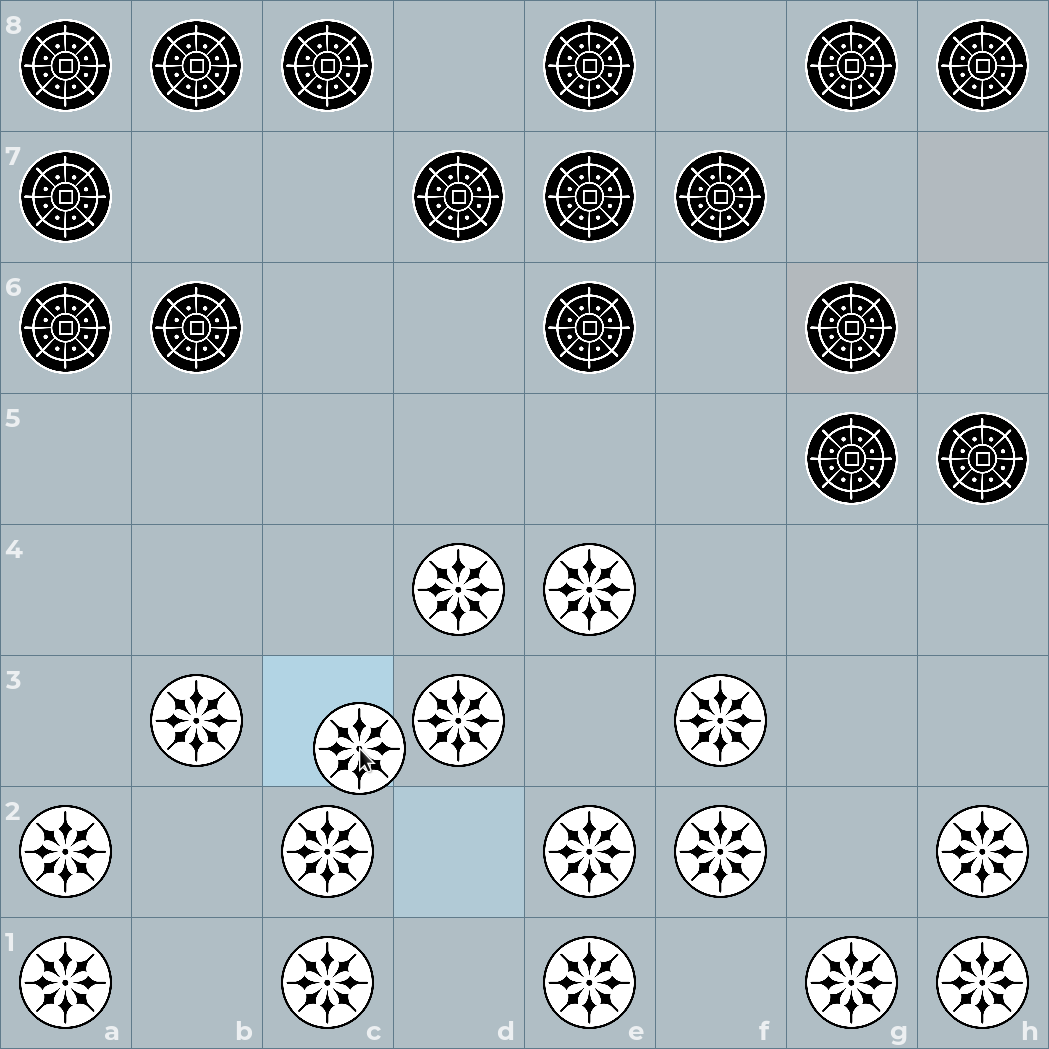
\includegraphics[width=0.4\textwidth]{data/guibtr.png}}

Naprogramujme to tak, že budeme mať triedu \vb{BoardView}, ktorá sa bude starať o vykresľovanie. Bude si pamätať obdĺžnik
\vb{SDL\_Rect screen}, do ktorého sa bude vykresľovať. Pre pohodlie si môže pamätať aj 
\vb{renderer}, keďže ju nikdy nebudeme chcieť renderovať inam. Premenná \vb{screen} sa bude meniť
volaním \vb{resize}. To je preto, že pri zmene veľkosti si možno budeš chcieť prepočítať
nejaké ďalšie veci, ktoré s veľkosťou okna súvisia. Napríklad rozmer šachovnice môžeš
nastaviť ako menší z dvoch rozmerov okna a pod. Bude si pamätať aj \link{\rootpath/sdl/pieces.png}{obrázok} hracích kameňov, 
aktuálnu polohu myši, či práve používateľ presúva kameň, či sa práve animuje a ak áno tak odkiaľ a kam atď. 
Hodia sa aj pomocné funkcie, ktoré pre políčko šachovnice vrátia pozíciu na obrazovke a naopak.
Jadro triedy by mohlo vyzerať takto:

\begin{lstlisting}
struct BoardView {
  SDL_Renderer* renderer;
  Board board;          // aktuálna pozícia
  SDL_Texture* pieces;  // textúra s bielym a čiernym kameňom
  uint8_t human;        // človek je Biely(0) / Čierny (1)
  bool flippedBoard;    // zobrazujem šachovnicu z pohľadu čierneho

  bool dragging, animating;  // ťahá hráč / počítač
  Square dragOrig;           // odkiaľ hráč začal ťah
  Move aMove;                // počítačový ťah, ktorý sa animuje
  const int animLen = 200;   // dĺžka animácie (ms)
  uint32_t animEndTime;      // kedy skončí aktuálna animácia

  SDL_Rect screen;     // obdĺžnik, kam sa vykresľujem
  int mouseX, mouseY;  // poloha myši
  ...                  // rôzne veci, ktoré potrebuješ pri vykresľovaní

  BoardView(SDL_Renderer* r);       // konštruktor
  void resize(SDL_Rect scr);        // nastaví všetko potrebné pri zmene okna
  void render();
  void operator+=(const Move& m);   // spustí animáciu ťahu protihráča

  void onMouseMotion(SDL_MouseMotionEvent& e);
  void onMouseDown(SDL_MouseButtonEvent& e);
  Move onMouseUp(SDL_MouseButtonEvent& e);
  ...                               // deštruktor, pomocné funkcie atď
};
\end{lstlisting}

V hlavnom cykle sa pri spracovaní eventov zavolajú funkcie \vb{onMouse...}, ktoré nastavia \vb{mouseX}, \vb{mouseY} a ošetria prípadný začiatok a koniec ťahania.
Špeciálne ak sa v \vb{onMouseUp} urobí ťah, tento sa vráti (inak vracia nejaký neprípustný ťah ako zarážku). V hlavnom programe sa tento ťah podhodí \vb{RandomPlayer}
z úlohy~\ref{uloha:randomplayer}, ktorý nájde ťah. Ten sa spätne pošle do zobrazovača cez \vb{operator+}: spustí sa animácia a keď skončí, aktualizuje sa pozícia.
Kus hlavného programu by mohol vyzerať takto (\vb{bv} je \vb{BoardView}, \vb{plr} je \vb{RandomPlayer}):\\

\begin{lstlisting}
case SDL_MOUSEBUTTONUP:
   if (bv.onMouseUp(e.button).from.legal() && // bv.onMouseUp vráti Move(from,to)
       bv.board.winner() == Empty) {          // ak je to legálny ťah a hra neskončila
     Move m = plr.findMove(bv.board);         // zisti ťah hráča
     bv += m;                                 // aktualizuj BoardView
   }
   break;
\end{lstlisting}

\begin{uloha}
  Naprogramuj grafické rozhranie, ako sme si ho tu opísali.
\end{uloha}




\chapter{Ako robiť viac vecí naraz}

Predpokladám, že ťa zarazilo, prečo som ti v minulej časti pri programovaní grafického prostredia povedal, aby sa hralo proti \vb{RandomPlayer},
keď už máme oveľa lepšieho \vb{AlphaBetaPlayer}. Možno si aj skúsil \hbox{\vb{AlphaBetaPlayer}} použiť. Ak nie, urob to teraz. Čo si zistil? 
V programe sa funkcia \vb{plr.findMove()} sa volá pri spracovaní udalostí v hlavnom cykle. To ale znamená, že ak \vb{plr.findMove()} trvá dlho, žiadne iné udalosti
sa počas toho času nespracovávajú a program sa na tú dobu ``zasekne'' (nereaguje na pohyby myšou, neprekresľuje okno, nič...). 

Aby sme to opravili, bolo by treba \vb{findMove} rozdeliť na krátke kúsky a vždy v jednej iterícii hlavného cyklu zavolať len jeden kúsok, napr. takto:

\begin{lstlisting}
struct AlphaBetaPlayer {
  struct MoveValue {...}

  std::mt19937 rnd;
  bool thinking,finished;

  AlphaBetaPlayer();

  void startThinking(const Board& b);
  void step();
  Move getResult();

  float eval(const Board& b);
};
\end{lstlisting}

V programe by sme namiesto \vb{findMove} zavolali funkciu \vb{startThinking}. Tam sa nastaví \vb{thinking=true} a \vb{finished=false}. Hlavnú robotu bude robiť
funkcia \vb{step}, ktorá vždy prehľadá kúsok stromu a prípadne nastaví premennú \vb{finished}. V programe by to mohlo vyzerať takto:

\begin{lstlisting}
  while (running) {
    SDL_Event e;
    while (SDL_PollEvent(&e)) {
      switch (e.type) {
        ...  // spracovať ostatné typy udalostí

        case SDL_MOUSEBUTTONUP:
          if (bv.onMouseUp(e.button).from.legal() && bv.board.winner() == Empty) 
            plr.startThinking(bv.board); // krátke volanie, ktoré nastaví začiatok
          break;
      }
    }
    ... // render
    if (plr.thinking) {
      while (!plr.finished) {  // tu voláme step(), kým máme čas v rámi zvoleného fps
          plr.step();
          uint32_t now = SDL_GetTicks();
          if (now >lastFrame + msPerFrame) break;
      }
      if (plr.finished) {  // ak skončil, prečítame výsledok a nastavíme novú pozíciu
         Move m = plr.getResult();
         bv+=m;
      }
    }
    ... // prípadne SDL\_Delay, ak zostáva čas
  }
\end{lstlisting}

Ako urobiť \vb{step}? Pripomeniem, že vo \vb{findMove} robí hlavnú časť práce rekurzívna funkcia 

\begin{lstlisting}
MoveValue search(const Boardr& b, int hlbka, float alpha, float beta)
\end{lstlisting}

v nej sa, v najjednoduchšej verzii, robí zhruba takýto cyklus

\begin{lstlisting}
  auto ms = b.legalMoves();
  for (int i = 0; i < ms.size(); i++) {
    Board bb = b;
    bb += ms[i];
    float v = -search(bb, hlbka - 1, -beta, -alpha).val;
    if (v > res.val) {
      res.val = v;
      res.m = ms[i];
    }
    if (res.val > alpha) alpha = res.val;
    if (alpha >= beta) break;
  }
\end{lstlisting}

Počas rekurzívneho volania sa postupne vytvára veľa svetov pre rôzne volania funkcie \vb{search}. Ak chceme, aby sa dala prerušiť, nemôžeme použiť
rekurziu, ale bude treba, aby sme si svety vytvárali sami. Urobíme si typ, v ktorom sa dá zapamätať jeden svet funkcie \vb{search}: musí obsahovať
všetky jej parametre aj lokálne premenné, napr.

\begin{lstlisting}
struct State {
  Board b;
  int hlbka;
  double alpha, beta;
  MoveValue res;
  std::vector<Move> ms;
  int i;
};
\end{lstlisting}

\vb{AlphaBetaPlayer} potom bude mať \vb{vector<State>}, ktorý bude slúžiť ako zásobník a
kde bude mať uložené všetky rozpracované svety. Volanie \vb{search} sa pozrie na posledný svet: ak sú ešte ťahy, ktoré treba 
spracovať, tak vyrobí nový svet a pridá ho na koniec vektora, v opačnom prípade upraví hodnoty v predposlednom svete a posledný zmaže.

\begin{uloha}
  Naprogramuj prehľadávanie tak, ako sme tu povedali, aby sa dalo v grafickom prostredí hrať.
\end{uloha}

Keď si vyriešil predchádzajúcu úlohu, asi vidíš nevýhody tohoto prístupu. Prerobiť existujúceho hráča tak, aby vedel 
bežať ``zároveň'' so spracovaním udalostí vyžaduje veľa práce. V našom prípade bola len jedna rekurzívna funkcia,
v ktorej sa robila všetka práca, ale
keby si mal program, kde je viacero funkcií, z ktorých každá môže pracovať dlho a vzájomne sa volajú, celé by to 
bolo ešte oveľa zložitejšie. 

\indexItem{Alg}{vlákno {\em (thread)}}
V C++ sa dá dosiahnuť, aby viacero funkcií bežalo ``naraz'', pomocou tzv. {\em vlákien} ({\em  threads}). 
V štandardnej knižnici \vb{<thread>} je šablóna \vb{thread}, ktorá umožňuje spúšťať funkcie nezávisle od
hlavného programu. Pozri si tento program:

%\vbox{
\begin{lstlisting}[label={l:thr.1}]
#include <iostream>
#include <thread>
using namespace std;

int result;

int collatz(int n) {
  int cnt;
  for (cnt = 0; n > 1; cnt++)
    if (n % 2 == 0) n = n / 2;
    else n = 3 * n + 1;
  return cnt;
}

void prvyDlhsi(int len) {
  for (result = 1; true; result++)
    if (collatz(result) > len) return;
}

int main() {
  int x;
  cin >> x;
  thread t(prvyDlhsi, x); @\ll1@
  cout << "Thread t pocita a program pokracuje" << endl; @\ll2@
  t.join(); @\ll3@
  cout << "Thread vypocital " << result << endl;
}

\end{lstlisting}
%}

Funkcia \vb{prvyDlhsi} vyráta prvé číslo, ktorého Collatzova postupnosť 
(pozri Úlohu~\ref{uloha:collatz}) je dlhšia ako zadané číslo. Napr. pre vstup $512$
je výsledok $4484223$. 

V hlavnom programe sa na riadku~\ref{l:thr.1-1} vyrobí premenná \vb{t}, ktorá je typu \vb{thread}.
Jej konštruktor je šablóna, ktorá ako prvý parameter zoberie niečo spustiteľné (funkciu, 
funktor, lambdu\footnote{pripomeň si kapitolu~\ref{sec:lambdy}}) 
a spustí to. Ďalšie parametre konštruktora sú parametre, ktoré
sa použijú pri spustení\footnote{To, že konštruktor \vb{thread} 
môže mať vždy iný počet parametrov, nie je nejaká záhadná špeciálna výnimka.
Pomocou šablón sa dajú spraviť funkcie, ktoré nemajú
pevne daný počet parametrov, ale pri každom volaní môžu mať 
iný počet. Keďže ale ten zápis je zo začiatku trochu neprehľadný a nikde sme to príliš nepotrebovali,
tak som ti o tom nepovedal. Ak ťa to zaujíma, treba si nájsť kľúčové slovo {\em parameter pack},
napr. 
\dlink{https://en.cppreference.com/w/cpp/language/parameter_pack}
}. V našom prípade sa spustí funkcia \vb{prvyDlhsi(x)}.
Akonáhle sa zavolá konštruktor, thread začne pracovať nezávisle a program 
pokračuje ďalej. Hlavný program aj novovytovrený thread majú spoločnú pamäť, takže
to môže vyzerať takto:

\begin{tikzpicture}[
    boxnode/.style={font=\robotomono,draw, minimum width = 3cm},
    popis/.style ={,anchor=east, left=5mm of #1}
  ]
  \def\nxtnd[#1](#2)(#3)#4{%
  \node[boxnode,#1,rect={#1}{}{#1}{#1}, below = 0cm of #2] (#3)  {#4};
  }

  \node[boxnode,rect={}{}{}{}] (pamat) at (0,0) {pamäť};
  \node[boxnode,rect={black}{}{black}{black}, below = 0cm of pamat] (start) { };
  \nxtnd[black](start)(result){result}
  \nxtnd[teal](result)(x){x}
  \nxtnd[teal](x)(t){t}
  \nxtnd[orange](t)(len){len}
  \nxtnd[orange](len)(n){n}
  \nxtnd[orange](n)(cnt){cnt}
  \node[boxnode,rect={black}{}{black}{}, below = 0cm of cnt] { };

  
  \node[popis={result}] (global) {globálna};  \draw[->, shorten >= 2ex] (global) -- (result);
  \node[teal,popis={x}] (main) {svet {\robotomono main()}};  \draw[->, shorten >= 2ex] (main) -- (x);
  \node[orange,popis={len}] (len1) {svet {\robotomono prvyDlhsi(len)}};  \draw[->, shorten >= 2ex] (len1) -- (len);
  \node[orange,popis={n}] (cnt1) {svet {\robotomono collatz(result)}};  \draw[->, shorten >= 2ex] (cnt1) -- (n);

  \node[teal,boxnode,rect={}{}{}{}] (mainthr0) at (4,0) {hlavný program};

  \node[boxnode,rect={teal}{}{teal}{teal}, below = 0cm of mainthr0] (mainthr1) { \rule{0mm}{1cm}};
  \node[boxnode,rect={teal}{}{teal}{teal}, below = 0cm of mainthr1] (mainthr2) { \vb{thread t(...);}};
  \nxtnd[teal](mainthr2)(mainthr3){\vb{cout << ... }};
  \node[boxnode,rect={teal}{}{teal}{},  below = 0cm of mainthr3]{\rule{0mm}{6ex}};
  
  \node[orange,boxnode,rect={}{}{}{}] (tthr) at (8,0) {thread {\robotomono t}};
  \node[orange,boxnode] (tthr1) at ($ (mainthr2) + (4.5,0) $) {{\robotomono prvyDlhsi(x)}};
  \nxtnd[orange](tthr1)(tthr2){...\rule{0mm}{2ex}};
  \nxtnd[orange](tthr2)(tthr3){collatz(result)};
  \node[boxnode,rect={orange}{}{orange}{},  below = 0cm of tthr3]{\rule{0mm}{2ex}};

  \draw[teal,->,shorten >= 2ex] (mainthr2) -- (tthr1);

\end{tikzpicture}

V pamäti je globálna premenná \vb{result}. Spustí sa hlavný program (funkcia \vb{main}), ktorý vytvorí svoj svet s lokálnou premennou \vb{x}.
Potom sa vyrobí premenná \vb{t} a keď sa volá konštruktor \vb{thread} na riadku~\ref{l:thr.1-1}, spustí sa zároveň aj funkcia \vb{prvyDlhsi}, ktorá si v pamäti vyrobí svoj svet
a potom zavolá funkciu \vb{collatz}, ktorá si opäť urobí vlastný svet. 
Hlavný program beží ďalej a môže pristupovať k premenným \vb{result}, \vb{t} a \vb{x}, vnútro funkcie \vb{collatz} môže pristupovať k 
premenným \vb{result}, \vb{n} a \vb{cnt}.

\indexItem{Prg}{\vb{thread}, \vb{join}, \vb{yield}}
So samotnou premennou typu \vb{thread} sa toho moc robiť nedá, ale je dôležité, aby ostala v pamäti po celý čas, kým beží funkcia threadu. 
Nasledujúci program zavolá funkciu \vb{rob}, ktorá spustí thread s lambdou, čo dlho počíta. Funkcia \vb{rob} vzápätí skončí,
takže sa zavolá deštruktor premennej \vb{t}. Lenže príslušná funkcia ešte beží, a preto program skončí s chybou.

\begin{lstlisting}
void rob() {
  thread t([](){
    int j = 0;
    for (int i = 0; i < 100000; i++) j += i;
  });
}

int main() { rob(); }
\end{lstlisting}

Jedna z mála metód typu \vb{thread} je \vb{join}, ktorá slúži presne na to, aby sa takýmto situáciám vyhlo. 
Ak sa zavolá \vb{t.join()} (ako v našom programe na riadku~\ref{l:thr.1-3}), aktuálny thread bude čakať, kým thread z 
premennej \vb{t} dobehne. Potom je už bezpečné zavolať deštruktor.

Pri threadoch síce hovoríme, že bežia naraz, ale v skutočnosti ti to nikto nesľúbi. Väčšina procesorov má viac jadier\footnote{%
  Počet jadier sa dá zistiť pomocou \prg!cout << thread::hardware_concurrency() << endl;!.
}a každé môže v jednom momente bežať jeden thread. Kým je v celom systéme menej threadov ako jadier, systém sa spravidla snaží dať nový thread na samostatné jadro, takže thready naozaj bežia naraz.
Ak je threadov viac, musí na jednom jadre bežať viacero threadov. Niektoré systémy to robia tak, že ich striedajú: nejaký krátky čas beží jeden, potom sa preruší,
beží ďalší a tak dookola. Ale na niektorých systémoch (spravidla sú to malé procesory, ktoré sa používajú do rôznych zariadení) je také prepnutie veľmi drahé.
Robia preto to, že zoberú jeden thread a ten beží, kým sa dá: to znamená až kým neskončí alebo nezačne čakať, či už na čítanie vstupu, nejakú udalosť, alebo kvôli
volaniu ako \vb{SDL\_Delay}. Potom zoberú iný thread, ktorý chce bežať a spustia zase ten. 
Štandard jazyka C++ sľubuje len to, čo je pre všetky tieto systémy spoločné. Treba mať preto na pamäti, že pri programovaní threadov nemáš žiadnu záruku
okrem toho, že ak nejaké jadro nemá čo robiť, tak sa na ňom spustí aspoň jeden nejaký thread, ktorý chce práve bežať. 

Ak si si spustil prvý príklad, tak pravdepodobne sa text
z riadku~\ref{l:thr.1-2} vypísal hneď a potom sa čakalo na dobehnutie funkcie \vb{prvyDlhsi} v druhom threade pri volaní \vb{join}. Ale pokojne to mohlo
byť aj naopak: začal by pracovať thread \vb{t} a kým má čo robiť (v našom prípade až kým neskončí), tak ho systém nechá bežať a až keď skončí, dá slovo hlavnému threadu.
Existuje funkcia \vb{this\_thread::yield()}, ktorá signalizuje systému \cmd{Pozri sa, či nechce náhodou bežať nejaký iný thread, ktorý už dlho čaká. Ak áno, 
radšej ma preruš a začni vykonávať ten}. Čo presne sa ale stane po zavolaní \vb{yield()}, to tiež závisí od systému (štandard C++ to nijak neurčuje). 

Užitočná je aj funkcia \vb{this\_thread::sleep\_for}, ktorá robí podobnú vec ako \vb{SDL\_Delay}, totiž uspí aktuálny thread na daný čas. Kvôli čitateľnosti je 
ale navrhnutá tak, že parameter nie je \vb{int}, ale  \vb{chrono::duration}, takže treba použiť \vb{\#inlcude <chrono>} a potom použiť napr.

\begin{lstlisting}
this_thread::sleep_for(chrono::milliseconds(1234));
\end{lstlisting}

Videl si, ako vyrobiť thread, v ktorom beží nejaká funkcia. Určite si si to všimol, ale pripomeniem, že návratová hodnota z tej funkcie sa zahodí a nemáš sa k nej ako dostať.
Thready medzi sebou komunikujú tak, že jeden thread napíše do nejakej spoločnej\footnote{buď je to globálna premenná ako v našom príklade, alebo napr. pošleš ako parameter
funkcie threadu pointer na premennú a pod.} premennej a druhý odtiaľ prečíta. Možno ti v hlave zablikala kontrolka: ak nemám žiadnu kontrolu nad tým, kedy ktorý thread vykonáva ktorú časť 
svojho programu, nemôže spoločné čítanie a zapisovanie do zdieľanej premennej spôsobiť problémy? Môže, hneď ti to ukážem. Zober si nasledovný program

\vbox{
  \begin{column}{0.45}
\begin{lstlisting}
#include <iostream>
#include <set>
using namespace std;
set<int> s;

void dump() {
  for (int x : s) cout << x << " ";
  cout << endl;
} 

void rob() {
  for (int i = 5; i < 100; i++) {
    s.erase((i - 5) % 100);
    s.insert(i % 100);
    if (i % 10 == 0) dump();
  }
}

int main() {
  for (int i = 0; i < 5; i++) 
    s.insert(i);
  rob();
}
\end{lstlisting}
  \end{column}
  \hfill
  \begin{column}{0.45}

Máme v ňom globálnu množinu (t.j. vyvážený vyhľadávací strom, pozri kapitolu~\ref{sect:stromy}) \vb{s}, do ktorej na začiatku dáme čísla $0,\ldots,4$. Funkcia \vb{rob}
vždy najmenšie číslo z množiny vyberie a vloží tam o jedno väčšie. Berieme iba zvyšky po delení 100, aby bol prehľadnejší výpis. Funkcia \vb{dump} vypíše obsah množiny,
Výstup programu vyzerá takto:\\


\begin{outputBox}
6 7 8 9 10 
16 17 18 19 20 
26 27 28 29 30 
36 37 38 39 40 
46 47 48 49 50 
56 57 58 59 60 
66 67 68 69 70 
76 77 78 79 80 
86 87 88 89 90 
0 96 97 98 99 
\end{outputBox}
  \end{column}
}


Teraz program zmeňme tak, že \vb{rob} pobeží v samostatnom threade a bude množinu meniť stále dookola. Hlavný program, po tom, čo spustí thread, vždy chvíľu počká
a vypíše obsah množiny. Keď program spustíš viackrát, výstupy sa budú líšiť, ale môžu vyzerať napr. takto:


\begin{column}{0.6}
\begin{lstlisting}
#include <chrono>
#include <iostream>
#include <set>
#include <thread>
using namespace std;
set<int> s;

void dump() {
  for (int x : s) cout << x << " ";
  cout << endl;
}

void rob() {
  for (int i = 5; i < 1000000; i++) {
    s.erase((i - 5) % 100);
    s.insert(i % 100);
  }
}

int main() {
  for (int i = 0; i < 5; i++) s.insert(i);
  thread t(rob);
  for (int i = 0; i < 10; i++) {
    this_thread::sleep_for(chrono::milliseconds(1));
    dump();
  }
  t.join();
}
\end{lstlisting}
  \end{column}
  \hfill
  \begin{column}{0.3}
\begin{outputBox}
73 24 25 26 25 26 
17 23 24 
1 7 8 
8 14 15 
59 65 66 67 
8 14 15 
44 50 51 52 
61 67 68 69 
3 9 10 11 
26 32 33 34 
\end{outputBox}
  \end{column}

Čo sa stalo? Jeden thread práve robil \vb{insert} alebo \vb{erase} na vyhľadávacom strome, 
kým druhý thread ho začal prechádzať, aby ho vypisoval. Ale počas toho, ako vypisoval strom, mu prvý thread
ten strom pod rukami menil, takže sa vypísalo niečo, čo v žiadnom momente v strome nebolo. Dostali sme sa k problému, ktorému sa hovorí
\indexItem{Prg}{vzájomné vylúčenie, \vb{mutex}} {\em vzájomné vylúčenie} ({\em mutual exclusion}):
máme program, v ktorom beží viacero threadov, ale je v  ňom časť (v našom prípade manipulácia s množinou \vb{s}), v ktorej nikdy nesmie pracovať viac threadov naraz. Základným
prostriedkom na zabezpečenie
vzájomného vylúčenia je typ \vb{mutex}, ktorý je definovaný v \vb{<mutex>}. Premenné typu \vb{mutex} sa nedajú priraďovať ani kopírovať, majú dve základné metódy: \vb{lock()} a \vb{unlock()}.
Ako fungujú je opäť najlepšie vidno na príklade. Zoberme program s troma threadmi, z ktorých každý chce postupne trikrát vypísať riadok. \\

\vbox{
\begin{lstlisting}
#include <iostream>
#include <string>
#include <thread>
#include <vector>
using namespace std;

void zdrz() {  // dajme tomu, ze tu niečo zložité počíta
  for (int i = 0, j = 0; i < 100000; i++) j += i;
}       

void pis(const string &s) {
  for (int i = 0; i < 3; i++) {
    for (char c : s) {
      cout << c;
      zdrz(); 
    } 
    cout << endl;
    zdrz();
  } 
} 

int main() {
  vector<thread> ts;
  ts.push_back(thread(pis, "kedsomisielcezhoru"));
  ts.push_back(thread(pis, "STRETOLSOMTAMPOTVORU"));
  ts.push_back(thread(pis, "!$^!?#!~^*?$!"));
  
  for (auto &t : ts) t.join();
} 
\end{lstlisting}
}

Keď ho spustíš, môže to vyzerať napr.

\begin{outputBox}
Sk!Te$Rd^Es!TOo?Lm#Si!Os~Mi^Te*Al?Mc$Pe!Oz
Th!Vo$Or^Ru!U?

#kS!Te~Rd^E*sT?oO$Lm!Si
O!sM$iT^Ae!Ml?P#cO!eT~zV^hO*oR?rU$u
!
S
kTeRdEsToOmLiSsOiMeTlAcMePzOhToVrOuR
U
\end{outputBox}  

Thready sa nepredvídateľne striedajú v tom, kto práve vypíše znak.
Zmeňme teraz program tak, že pridáme \vb{\#include <mutex>}, vyrobíme globálnu premennú \vb{mutex m} a funkciu \vb{pis} zmeníme takto:

\vbox{
\begin{lstlisting}[label={l:thr.2}]
void pis(const string &s) {
  for (int i = 0; i < 3; i++) {
    m.lock(); @\ll1@
    for (char c : s) {
      cout << c;
      zdrz(); 
    } 
    cout << endl;
    m.unlock(); @\ll2@
    zdrz();
  } 
} 
\end{lstlisting}
}

Hlavný program sa nezmení, spustí tri thready. Prvý thread (nevieme, ktorý, ale jeden z nich to bude, nazvime ho $A$), sa dostane na riadok~\ref{l:thr.2-1} a zavolá \vb{m.lock()}. Tým sa mutex \vb{m}
``zamkne''. Ďalší thread, dajme tomu, že $B$, ktorý dorazí na riadok~\ref{l:thr.2-1}, tiež zavolá \vb{m.lock()}. 
Mutex \vb{m} je už ale zamknutý, preto systém thread $B$ preruší a zapamätá si, že $B$ čaká na mutex \vb{m}. Podobne aj tretí thread. Po čase thread $A$ dokončí vypisovanie reťazca
a príde na riadok~\ref{l:thr.2-2}, kde zavolá \vb{m.unlock()}. Mutex sa tým ``odomkne'', systém zistí, že nejaké thready na mutex \vb{m} čakali, vyberie z nich jeden, napr. $B$, mutex zamkne
a thread $B$ pustí bežať. Z pohľadu threadu $B$ sa nič nestalo: zavolal \vb{m.lock()} a pokračoval ďalej (medzitým chvíľu spal, ale to si nijak nevšimol). 

Na to, aby to celé fungovalo, musí byť \vb{unlock()} podporovaný
operačným systémom. Treba totiž, aby sa celá postupnosť \cmd{Odomkni mutex, zisti, či na ňom nejaké thready čakali, ak áno vyber jeden z nich, pusti ho bežať a zamkni mutex} vykonala
{\em atomicky}, t.j. ako keby to bola jedna inštrukcia. Inak by nejaký iný bežiaci thread 
mohol nájsť odomknutý mutex v tom krátkom čase medzi tým, keď 
už systém vybral nový thread na bežanie,  ale ešte nezamkol mutex.

Keď takto upravený program spustíš, už bude pracovať správne, vypíše sa napr.

\begin{outputBox}
!$^!?#!~^*?$!
STRETOLSOMTAMPOTVORU
kedsomisielcezhoru
kedsomisielcezhoru
STRETOLSOMTAMPOTVORU
!$^!?#!~^*?$!
kedsomisielcezhoru
STRETOLSOMTAMPOTVORU
!$^!?#!~^*?$!
\end{outputBox}

Akonáhle sa nejaký thread dostal do tej časti programu, v ktorej sa vypisuje, dokončil vypisovanie celého riadku bez prerušenia. Ostatné thready, ktoré by medzitým chceli 
vypisovať, poslušne čakali, kým na ne príde rad.

Použitie mutexu je veľmi náchylné na robenie chýb, ktoré sa veľmi zle hľadajú.
Keby napr. funkcia \vb{pis} zavolala \vb{return} predtým ako zavolá
\vb{m.unlock()}, mutex by ostal zamknutý a ostatné thready by sa nikdy
nedostali k slovu. Takisto mutex sa musí používať v správnom poradí, t.j.
nejaký thread zavolá \vb{lock()} a potom ten istý thread zavolá \vb{unlock()}.
Volať \vb{unlock()} z iného threadu, volať dvakrát za sebou \vb{lock()} z toho
istého threadu a pod. môže spôsobiť záhadné chyby, ktoré sa neprejavia pri
každom behu programu, ale iba občas. Preto sa \vb{mutex} používa zriedkakedy priamo,\indexItem{Prg}{\vb{lock\_guard}}
ale častejšie prostredníctvom \vb{lock\_guard}. Typ \vb{lock\_guard} v konštruktore 
dostane ako parameter premennú typu \vb{mutex} a ešte v konštruktore na ňu zavolá \vb{lock()}.
V deštruktore sa potom zavolá \vb{unlock()}. To znamená, že ak vyrobíš premennú typu
\vb{lock\_guard}, program za ňou je chránený príslušným mutexom, až kým sa nezavolá jej deštruktor.
Napr. funkcia \vb{pis} by sa dala napísať takto:

\vbox{
\begin{lstlisting}[label={l:thr.3}]
void pis(const string &s) {
  for (int i = 0; i < 3; i++) {
    { @\ll1@
      lock_guard guard(m);@\ll2@
      for (char c : s) {
        cout << c;
        zdrz();
      }
      cout << endl;
    }@\ll3@
    zdrz();
  }
}
\end{lstlisting}
}

Zložený príkaz na riadkoch \ref{l:thr.3-1} a \ref{l:thr.3-3} vytvára svet, v ktorom 
žije premenná \vb{guard}. Pri jej vytvorení sa na riadku \ref{l:thr.3-2} zamkne mutex \vb{m}
a v jej deštruktore na riadku~\ref{l:thr.3-3} sa odomkne. Príjemné na tom je, že ak 
niekedy v budúcnosti zmeníš program tak, že napr. niekedy počas vypisovania zavoláš \vb{return},
deštruktor \vb{guard} sa zavolá aj tak a nezanesieš si do programu ozaj nepríjemnú chybu.

Niekedy je ombedzenie, že ten istý thread, čo zavolal \vb{lock()} musí zavolať aj \vb{unlock()}
dosť nepríjemné. V novších\footnote{od štandardu C++20 vyššie, takže kompilátoru 
chceš povedať napr. \vb{-std=c++20}}  štandardoch C++ je
aj všeobecnejší mechanizmus, tzv. {\em semafór}. Používa sa podobne ako \vb{mutex}: \indexItem{Prg}{\vb{counting\_semapphore}}
pridá sa \vb{\#include <semaphore>} a vyrobí sa premenná typu \vb{counting\_semaphore}
niekde, kde ju všetky thready vidia (napr. ako globálna premenná).
Semafór\footnote{Pôvodne ho vymyslel E. W. Dijkstra a predstavoval si pri tom
také železničné návestie s ukazovateľom, ktorý sa môže posúvať hore a dolu.} je
vlastne počítadlo, ktoré sa dá atomicky zvyšovať a znižovať. V konštruktore
dostane štartovaciu hodnotu. Ak máš premennú napr. \vb{counting\_semaphore s(4)},
tak ktorýkoľvek thread môže hocikedy zavolať \vb{s.acquire()}, čím sa hodnota počítadla zníži, alebo
\vb{s.release()}, čím sa hodnota počítadla zvýši. Hodnota nikdy nebude záporná
a ak nejaký thread zavolá \vb{s.acquire()} vtedy, keď hodnota počítadla bola $0$, 
systém ho preruší a zapamätá si, kde čaká. Keď potom nejaký iný thread zavolá 
\vb{s.release()}, tak podobne ako pri mutexoch sa atomicky vyberie jeden z čakajúcich threadov
a spustí sa.

Preože semafór môže jeden thread zvýšiť a druhý znížiť, používajú sa na dohadovanie medzi threadmi:
jeden thread na semafóre zaspí (spraví \vb{acquire()} na nulovom počítadle) a čaká, kým ho druhý zobudí (zavolá \vb{release()}).

Typický príklad na komunikáciu threadov je \indexItem{Alg}{{\em producer-consumer}} tzv. {\em producer-consumer} problém. 
Dajme tomu, že chceš vyrobiť dataset, v ktorom budú tváre ľudí z obrázkov na internete.
Máš jednu funkciu, ktorá vie stiahnuť náhodný obrázok z internetu a druhú funkciu, ktorá vie zobrať obrázok a vyrezať z neho oblasť s tvárou.
Problém je, že obe tie funkcie môžu trvať rôzne dlho. Raz treba dlho čakať, kým sa podarí nejaký obrázok stiahnuť a inokedy sa obrázky
chrlia rýchlo, ale ich spracovanie trvá dlho. Vyriešime to tak, že si urobíme buffer, do ktorého bude prvá funkcia (nazvime ju \vb{producer})
ukladať obrázky a druhá funkcia (nazvime ju \vb{consumer}) z neho bude čítať. Na buffer môžeme použiť \indexItem{Prg}{\vb{deque}} napr. triedu \vb{deque} z STL; \vb{deque}
sa podobá \vb{vector}u, ale vieme efektívne pridávať a uberať z oboch koncov, t.j. máme
operácie \vb{push\_back}, \vb{push\_front}, \vb{pop\_back}, \vb{pop\_front}, \vb{front} a \vb{back},
ktoré vedia pridávať, uberať a pristupovať k prvkom na začiatku a konci poľa\footnote{Premysli si, ako by si si takú triedu mohol vyrobiť sám.}. 
Chceme, aby si \vb{producer} pracoval a keď získa obrázok, 
uloží ho na koniec buffra. Podobne \vb{consumer} si postupne číta z buffra obrázky a spracováva ich. Ak je buffer prázdny, \vb{consumer} by mal
zaspať a zobudiť sa, až keď bude mať robotu. Podobne nechceme, aby buffer príliš narástol, takže ak je v ňom viac ako $n$ obrázkov,
\vb{producer} by mal zaspať a zobudiť sa, až keď bude v buffri miesto. No a ešte by sme chceli aj takú možnosť, aby bežalo naraz viac threadov
\vb{producer} a viac threadov \vb{consumer}.

Aby sme zabezpečili, že buffer sa nikdy nepokazí, budeme si prístup k nemu chrániť mutexom \vb{mtx}. Zároveň si jednotlivé \vb{producer} a \vb{conumer}
thready budú signalizovať, kedy majú zaspať a kedy sa majú zobudiť. Na to použijeme dva semafóry. Semafór \vb{prazdny} bude mať vždy takú hodnotu
počítadla, koľko je v buffri vecí. Začína teda s nulou, \vb{consumer} ho zníži a \vb{producer} ho zvýši. Druhý semafór, \vb{plny}, bude mať hodnotu počítadla
vždy takú koľko je v buffri voľných miest. Celý systém by vyzeral takto:

\hfill
\begin{tikzpicture}[
    head/.style={font=\robotomono},
    point/.style={circle,inner sep=0pt,minimum size=2pt,fill=red},
    lock/.style={fill=orange!40!white, draw=orange, very thick, minimum size=4mm,rectangle},
    unlock/.style={fill=teal!40!white, draw=teal, very thick, minimum size=4mm,circle},
    work/.style={draw=black, thin, fill=yellow!10!white, minimum width=24mm, font=\robotomono},
    ctrl/.style={thick, shorten <= 2pt, shorten >= 2pt, rounded corners},
    skip loop/.style={->, to path={-- ++(#1,0) |- (\tikztotarget)}}
]
    \matrix[column sep = 4.5cm, row sep = 8mm]{
    \node[head] (p0) {producer}; & \node[head] (c0){consumer}; \\
    \node[point] (p1){} ; & \node[point] (c1){}; \\
    \node[lock] (p2) {}; & \node[lock] (c2){}; \\
    \node[lock] (p3) {}; & \node[lock] (c3){}; \\
    \node[work] (p4) {vyrob}; & \node[work] (c4){spracuj}; \\
    \node[unlock] (p5) {}; & \node[unlock] (c5){}; \\
    \node[unlock] (p6) {}; & \node[unlock] (c6){}; \\
    \coordinate (p7) ; & \coordinate (c7);\\
  };

  \path (p7) edge [red, ctrl, skip loop = -22mm] (p1)
        (c7) edge [red, ctrl, skip loop = 22mm] (c1);
         
  \foreach \s in {p,c} { \foreach \n/\m in {0/2,2/3,3/4,4/5,5/6} { \draw[red, ctrl, -> ] (\s\n) -- (\s\m);}}

  \draw[red, ctrl]   (p6) -- (p7) -- ++(-5mm,0)
                     (c6) -- (c7) -- ++(5mm,0);

  \path (p5) edge [dashed, teal, ctrl, skip loop = -15mm] (p3)
        (c5) edge [dashed, teal, ctrl, skip loop = 15mm] (c3);

  
  \def\lblr#1(#2)[#3]#4{\node[#3, anchor = west] at (#2) {\raisebox{#1 5mm}{\hspace*{2mm}\robotomono\small #4}}}
  \def\lbll#1(#2)[#3]#4{\node[#3, anchor = east] at (#2) {\raisebox{#1 5mm}{\robotomono\small #4\hspace*{2mm}}}}

  \lblr-(p6)[teal]{prazdny.raise()};
  \lblr+(p5)[teal]{mtx.unlock()};
  \lblr+(p2)[orange]{plny.acquire()};
  \lblr-(p3)[orange]{mtx.lock()};

  \lbll-(c6)[teal]{plny.raise()};
  \lbll+(c5)[teal]{mtx.unlock()};
  \lbll+(c2)[orange]{prazdny.acquire()};
  \lbll-(c3)[orange]{mtx.lock()};

  \path (p6) edge[teal, dashed, ctrl, ->, out=10, in=200] (c2)
        (c6) edge[teal, dashed, ctrl, ->, out=170, in=340] (p2);

\end{tikzpicture}
\hfill~

Na tento obrázok  sa treba dobre zadívať a presvedčiť sa, že je to naozaj v poriadku, nech by thready pracovali v akomkoľvek poradí: 
keď si \vb{producer} zamkne \vb{mtx}, v buffri je voľné miesto, keď si 
\vb{consumer} zamkne \vb{mtx}, je v buffri aspoň jedna vec. \indexItem{Alg}{{\em deadlock}}Zároveň nikdy nenastane {\em deadlock}, t.j. situácia, keď všetky thready spia a 
čakajú a celý program sa tým pádom zasekne.

Keď už máme program takto navrhnutý, napísať ho je ľahké. Tu urobíme iba simuláciu, namiesto vyrábania aj spracovávania dáme iba čakanie.
Najprv si pripravíme knižnice a globálne premenné. Tu si len treba všimnúť, že \vb{counting\_semaphore} je šablóna, ktorá ako parameter
dostane očakávanú maximálnu hodnotu počítadla\footnote{Ako sme už spomínali, šablóny môžu mať okrem typov aj celočíselné parametre, napr.
pre šablónu \prg!template <typename T, int N> int f(T x) {return (int)(x) + N;}! je \prg!f<float, 4>! funkcia, ktorá zoberie parameter typu \prg!float!,
pretypuje ho na \prg!int! a priráta k nemu $4$. Hodnota $4$ je v tele funkcie fixovaná, pre rôzne hodnoty sa zo šablóny vyrobia rôzne funkcie.}. Je to viac-menej iba
kvôli možnej optimalizácii, v programe môže počítadlo narásť aj viac.


\begin{lstlisting}
#include <chrono>
#include <deque>
#include <iostream>
#include <mutex>
#include <random>
#include <semaphore>
#include <thread>
#include <vector>
using namespace std;
const int N = 10;

deque<int> buffer;

counting_semaphore<N> plny(N), prazdny(0);
mutex mtx;
\end{lstlisting}

Pre jednoduchosť povieme, že \vb{producer} aj \vb{consumer} budú bežať stále. V naozajstnom programe by si tam chcel mať nejaký spôsob, ako ich zastaviť (napr. zdieľanú
premennú, do ktorej sa zapíše, ak treba skončiť). V našom prípade si \vb{producer} vymyslí číslo, chvíľu počká a uloží ho na koniec buffra.

\vbox{
\begin{lstlisting}
void producer(int id) {
  mt19937 rnd{random_device{}()};

  while (true) {
    int num = rnd() % 1000;
    this_thread::sleep_for(chrono::milliseconds(rnd() % 1000));
    plny.acquire();
    mtx.lock();
    cout << "Producer " << id << " vyrobil " << num << endl;
    buffer.push_back(num);
    mtx.unlock();
    prazdny.release();
  }
}
\end{lstlisting}
}

Podobne napíšeme \vb{consumer}:

\vbox{
\begin{lstlisting}
void consumer(int id) {
  mt19937 rnd{random_device{}()};

  while (true) {
    prazdny.acquire();
    mtx.lock();
    int num = buffer.front();
    buffer.pop_front();
    cout << "Consumer " << id << " spracoval " << num << endl;
    mtx.unlock();
    plny.release();
    this_thread::sleep_for(chrono::milliseconds(rnd() % 1000));
  }
}
\end{lstlisting}
}

Hlavný program len spustí thready:

\begin{lstlisting}
int main() {
  vector<thread> ts;
  for (int i = 1; i <= 4; i++) ts.push_back(thread(producer, i));
  for (int i = 1; i <= 2; i++) ts.push_back(thread(consumer, i));
  for (auto &t : ts) t.join();
}
\end{lstlisting}

Toto by nateraz mohlo stačiť na základný prehľad o multithreadovom programovaní. Keď sa vrátime k nášmu \btr projektu: namiesto zložitého prerábania hráča, ako na začiatku tejto 
kapitoly, je jednoduchšie zaobaliť existujúceho hráča do threadu. V konštruktore sa spustí thread, ktorý spí na semafóre. Keď treba rátať ťah, semafór sa zdvihne a thread počíta.
Hlavný program pri spracovaní udalostí kontroluje, či hráčov thread už dorátal ťah.

\begin{uloha}
  Naprogramuj multithreadového hráča.
\end{uloha}


\chapter{Dedičnosť}
\label{sect:dedicnost}

Náš \btr projekt celkom dobre postupuje a chýba už iba GUI\footnote{{\em
Graphical User Interface}: gombíky, scrollovátka a iné grafické ovládátka}. Na
to existuje nepreberné množstvo rôznych knižníc, 
od úplne minimalistických ako napr. \link{https://github.com/rxi/microui}{microUI}
až po obrovské kolosy ako \link{https://doc.qt.io/qt-6/qtgui-index.html}{Qt},
ale opäť kvôli vysvetleniu
nejakých ďalších vecí by som chcel, aby sme si jednoduchú GUI knižnicu
naprogramovali. Spravíme iba veľmi jednoduchý základ, s ktorým budeme 
vedieť vyrobiť takýto program:

\vskip 3ex
\centerline{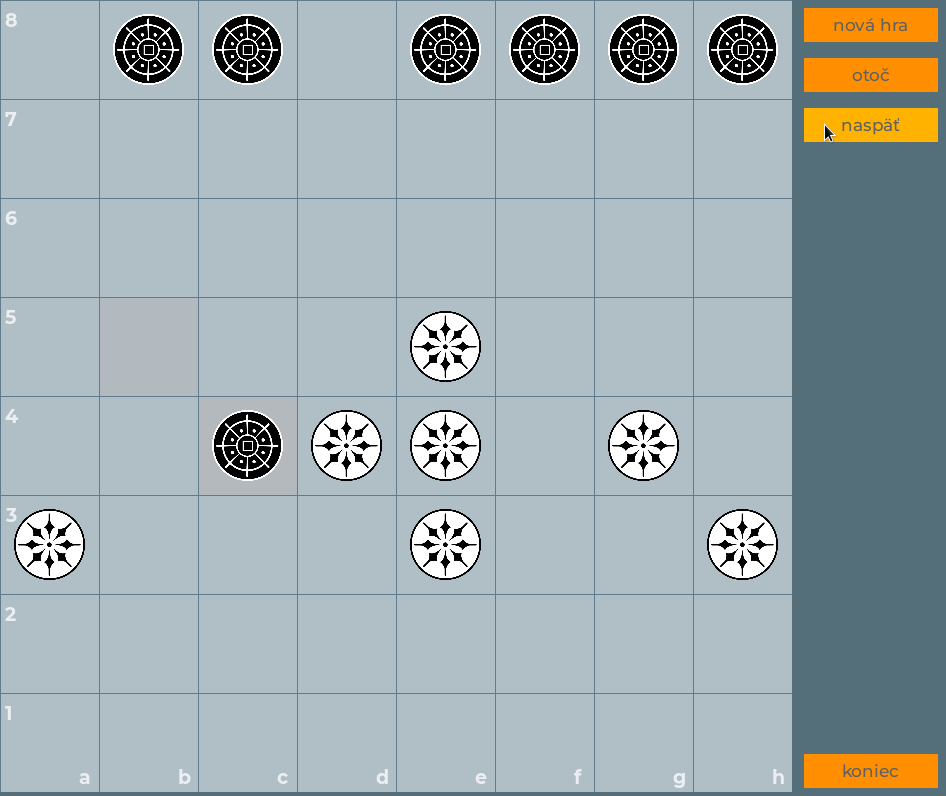
\includegraphics[width=0.55\textwidth]{data/gui.png}}

V našej knižnici bude celé okno rozdelené na {\em widgety}. Widget bude trieda,
ktorá spravuje časť okna, vie sa prispôsobiť zmenenej veľkosti, vie reagovať na
kliknutia myšou (prípadne iné udalosti, napr. stlačenie klávesy) a vie sa
vykresliť do SDL renderera. Príkladom widgetu je naša trieda \vb{BoardView} z
kapitoly~\ref{sect:SDL}. Iný widget by mohol byť napr. \vb{Button}, ktorý predstavuje 
jeden gombík a stará sa o to, aby sa naňho dalo kliknúť. Ďalší typ widgetov sa stará o rozmiestňovanie iných widgetov.
Widget \vb{Layout} si pamätá zoznam widgetov a prepočítava ich veľkosť a umiestnenie.
V našom prípade chceme mať ako hlavný widget horizontálny layout, ktorý obsahuje dva widgety:
\vb{BoardView} a vertikálny layout. Ten obsahuje päť widgetov: tri gombíky, 
jeden widget na vyplnenie miesta a ďalší gombík. 

Takže stačí napísať pre každý widget príslušnú triedu, poskladať to celé dokopy a hotovo.
Vidno tu ale dva problémy. Po prvé, je veľa funkcionality, ktorá je pre všetky (prípadne niektoré)
widgety spoločná. Napr. každý widget si má pamätať \vb{SDL\_Rect rect}, ktorý na obrazovke zaberá.
Takisto môže mať okraje nejakej hrúbky. Takže všetky widgety budú mať metódu 
\hbox{\vb{resize(SDL\_Rect newRect)}}, v ktorej bude

\begin{lstlisting}
  rect = newRect;
  rect.x += padding;
  rect.y += padding;
  rect.w -= 2 * padding;
  rect.h -= 2 * padding;
\end{lstlisting}

Navyše widgety \vb{Layout} ešte prerátajú rozmery svojich vnútorných widgetov a zavolajú
ich \vb{resize}. Postupne sa bude nabaľovať viac a viac kódu, ktorý je na veľa miestach rovnaký,
čo je oštara. Na druhý problém narazíš, ak začneš rozmýšľať, ako naprogramovať typ \vb{Layout}.
Potrebuje mať totiž zoznam svojich vnútorných widgetov, ktoré môžu byť rôznych typov. 
Ukážem ti, že na oba tieto problémy je dobré riešenie mechanizmus, ktorému sa v C++
hovorí {\em dedičnosť}.

Opäť poďme od začiatku. Dajme tomu, že by si mal triedu

\begin{lstlisting}
struct Widget {
  int x, y;
  void render();
};
\end{lstlisting}

Keď urobíš premennú \vb{Widget w}, v pamäti to bude vyzerať takto:

\begin{tikzpicture}[
    boxnode/.style={font=\robotomono,draw, minimum width = 5cm},
    popis/.style ={,anchor=east, left=5mm of #1}
  ]
  \def\nxtnd[#1](#2)(#3)#4{%
  \node[boxnode,#1,rect={#1}{}{#1}{#1}, below = 0cm of #2] (#3)  {#4};
  }

  \node[boxnode,rect={}{}{}{}] (pamat) at (0,0) {dáta};
  \node[boxnode,rect={black}{}{black}{black}, below = 0cm of pamat] (start) { };
  \nxtnd[black](start)(x){int Widget::x}
  \nxtnd[black](x)(y){int Widget::y}
  \node[boxnode,rect={black}{}{black}{}, below = 0cm of y] { };

  \node[popis={x}] (w) {{\robotomono w}};  \draw[->, shorten >= 2ex] (w) -- (x);

  \node[black,boxnode,rect={}{}{}{}] (prog0) at (8,0) {program};
  \node[boxnode,rect={black}{}{black}{black}, below = 0cm of prog0] (ps) { };
  \nxtnd[black](ps)(f){Widget::render()}
  \node[boxnode,rect={black}{}{black}{}, below = 0cm of f] { };
\end{tikzpicture}

To znamená, že každá premenná typu \vb{Widget} má v pamäti dve premenné \vb{int}
a navyše je v programe funkcia \vb{Widget::render()}.\indexItem{Prg}{dedenie}
Teraz môžeš urobiť triedu \vb{Button}, ktorá bude mať všetko to, čo \vb{Widget}
a aj niečo navyše. Hovoríme, že \vb{Button} dedí od \vb{Widget} a zapíše sa to takto:

\begin{lstlisting}
struct Button : Widget {
  string label;
  void render();
  void click();
};
\end{lstlisting}

Každá premenná typu \vb{Button} bude mať tri premenné: dve zdedené od \vb{Widget}
a jednu novú. V programe budú tri funkcie, takže \vb{Button b;} bude vyzerať takto:

\begin{tikzpicture}[
    boxnode/.style={font=\robotomono,draw, minimum width = 5cm},
    popis/.style ={,anchor=east, left=5mm of #1}
  ]
  \def\nxtnd[#1](#2)(#3)#4{%
  \node[boxnode,#1,rect={#1}{}{#1}{#1}, below = 0cm of #2] (#3)  {#4};
  }

  \node[boxnode,rect={}{}{}{}] (pamat) at (0,0) {dáta};
  \node[boxnode,rect={black}{}{black}{black}, below = 0cm of pamat] (start) { };
  \nxtnd[black](start)(x){int Widget::x}
  \nxtnd[black](x)(y){int Widget::y}
  \nxtnd[teal](y)(label){string Button::label}
  \node[boxnode,rect={black}{}{black}{}, below = 0cm of label] { };

  \node[popis={x}] (b) {{\robotomono b}};  \draw[->, shorten >= 2ex] (b) -- (x);

  \node[black,boxnode,rect={}{}{}{}] (prog0) at (8,0) {program};
  \node[boxnode,rect={black}{}{black}{black}, below = 0cm of prog0] (ps) { };
  \nxtnd[black](ps)(f){Widget::render()}
  \nxtnd[teal](f)(g){Button::render()}
  \nxtnd[teal](g)(h){Button::click()}
  \node[boxnode,rect={black}{}{black}{}, below = 0cm of h] { };
\end{tikzpicture}

Môžeš si to vyskúšať, program

\begin{lstlisting}[label={l:ded.1}]
#include <iostream>
#include <string>
using namespace std;

struct Widget {
  int x, y;
  void render() { cout << "Widget::render " << x << " " << y << endl; }
};

struct Button : Widget {
  string label;
  void render() { cout << "Button::render " << x << " " << y << " " << label << endl; } @\ll1@
  void click() { cout << "Button::click " << x << " " << y << " " << label << endl; }
};

int main() {
  Widget w; 
  w.x = 12; w.y = 42; w.render();

  Button b;
  b.x = 17; b.y = 47; b.label = "kikirikí"; b.render(); b.click();
}
\end{lstlisting}

vypíše 

\begin{outputBox}
Widget::render 12 42
Button::render 17 47 kikirikí
Button::click 17 47 kikirikí
\end{outputBox}

Teraz z programu vymaž riadok~\ref{l:ded.1-1}, 
teda v programe už nebude funkcia \vb{Button::render()}. Mala by sa vypísať chyba, že 
\vb{b.render()} volá neexistujúcu funkciu \vb{Button::render()}, ale chyba sa nevypíše.
Keď upravený program spustíš, vypíše sa

\begin{outputBox}
Widget::render 12 42
Widget::render 17 47
Button::click 17 47 kikirikí
\end{outputBox}

Čo sa stalo? Pri dedení sa totiž dedia nielen premenné, ale aj funkcie. Je to podobne ako
s lokálnymi premennými: ak existuje funkcia z daného typu (napr. \vb{Button::render()}),
použije sa tá. Ak neexistuje, kompilátor sa skúsi pozrieť na typ, z ktorého sa dedilo,
a použije funkciu odtiaľ
(napr. \vb{Widget::render()}). Keď sa nad tým zamyslíš, dáva to zmysel: pretože
\vb{Button} obsahuje všetky premenné, ktoré má \vb{Widget}, tak každá funkcia, ktorá
by pracovala na premennej typu \vb{Widget} môže rovnako dobre pracovať na premennej
typu \vb{Button}. V programe sa preto zavolala funkcia \vb{Widget::render()} na
premennú \vb{b}.

Teraz by sa zdalo, že to ale nesedí: v kapitole~\ref{sect:stack} sme hovorili, 
že metódy sú funkcie, ktoré majú ``neviditeľný'' prvý parameter \vb{this}, takže 
v našom prípade máme funkcie

\begin{lstlisting}
void Widget::render (Widget* this) {...}
void Button::render (Button* this) {...}
\end{lstlisting}

Keď sa teda zavolá \vb{Widget::render} namiesto \vb{Button::render}, tak sa 
musí aj zmeniť typ pointra z \vb{Button*} na \vb{Widget*}. To sa aj v skutočnosti udeje
a nielen pri volaní metód. Opäť, keď sa nad tým zamyslíš, tak \vb{Widget*} je
\cmd{adresa v pamäti, kde sa začínajú dáta nejakej premennej typu {\robotomono Widget}}.
To isté ale platí aj pre \vb{Button*}: je to adresa v pamäti, kde sa začínajú dáta
pre nejakú premennú typu \vb{Widget}. Že za nimi sa potom nachádzajú ďalšie dáta tak,
že je to celá premenná typu \vb{Button}, to je už druhá vec.
Preto je vždy možné pointer na ``väčší'' typ (napr. \vb{Button}) použiť tam, kde
sa vyžaduje pointer na ``menší'' typ (napr. \vb{Layout}).

Zase si to vyskúšaj. Vráť naspäť vymazaný riadok tak, aby \vb{Widget} aj \vb{Button}
mali vlastnú funkciu \vb{render} a hlavný program zmeň takto:

\begin{lstlisting}[label={l:ded.2}]
int main() {
  Button *b = new Button;
  b->x = 17;  b->y = 47; b->label = "kikirikí";
  b->render(); @\ll1@

  Widget *q = b; @\ll2@
  q->render(); @\ll3@
}
\end{lstlisting}

Vypíše sa

\begin{outputBox}
Button::render 17 47 kikirikí
Widget::render 17 47
\end{outputBox}

Prečo? Premenná \vb{b} je typu \vb{Button*}, preto volanie \vb{b->render()} na 
riadku~\ref{l:ded.2-1} zavolá funkciu \vb{Button::render}.
Premenná \vb{q} je typu \vb{Widget*}. Na riadku~\ref{l:ded.2-2} sa do nej priradí 
\vb{b}, takže \vb{q} ukazuje na to isté miesto v pamäti, kde je uložená premenná \vb{*b}.
Volanie \vb{q->render()} na riadku~\ref{l:ded.2-3} preto zavolá \vb{Widget::render}
na premennej typu \vb{Widget}, ktorá vznikne ``orezaním'' \vb{*b} do typu \vb{Widget}
(t.j. zabudne sa na \vb{b->label}).

S týmto mechanizmom máme jednu dobrú a jednu zlú správu. Dobrá správa je, že v našom type
\vb{Layout} by sme vedeli spraviť pole rôznych widgetov. Ak všetky widgety budú nejakým 
spôsobom\footnote{aj nepriamo, napr. \vb{Layout} bude dediť z \vb{Widget} a \vb{HLayout}
bude dediť z \vb{Layout}}
dediť zo základného typu \vb{Widget} tak môžeme spraviť \vb{vector<Widget *> children},
ktorý bude obsahovať pointre na widgety, ktoré môžu byť gombíky, ďalšie layouty a pod.

Zlá správa je, že ak potom zavoláme napr.

\begin{lstlisting}
  for (int i = 0; i < children.size(); i++) 
    children[i]->render();
\end{lstlisting}

Tak sa na každé z detí zavolá \vb{Widget::render}. Všetky sú totiž typu \vb{Widget*}
a kompilátor nemá ako vedieť, že kedysi dávno sme tam priradili iné typy. 
Chcelo by to nejaký mechanizmus, ktorým by sa zapamätalo, aký typ má ktoré z detí, aby potom
sa volala metóda \vb{render} z príslušného typu. \indexItem{Prg}{virtuálne metódy}
Tento mechanizmus sa volá {\em virtuálne metódy}. 
Zober si takto zmenenú triedu (pred deklaráciu \vb{render}
som pridal slovo \vb{virtual})

\begin{lstlisting}
struct Widget {
  int x, y;
  virtual void render();
};

void Widget::render() { cout << "Widget::render " << x << " " << y << endl; }
\end{lstlisting}

Keď teraz vyrobíš premennú \vb{Widget w}, v pamäti to bude vyzerať takto:

\begin{tikzpicture}[
    boxnode/.style={font=\robotomono,draw, minimum width = 5cm},
    popis/.style ={,anchor=east, left=5mm of #1}
  ]
  \def\nxtnd[#1](#2)(#3)#4{%
  \node[boxnode,#1,rect={#1}{}{#1}{#1}, below = 0cm of #2] (#3)  {#4};
  }

  \node[boxnode,rect={}{}{}{}] (pamat) at (0,0) {dáta};
  \node[boxnode,rect={black}{}{black}{black}, below = 0cm of pamat] (start) { };
  \nxtnd[orange](start)(vt){Widget::\_vptr}
  \nxtnd[black](vt)(x){int Widget::x}
  \nxtnd[black](x)(y){int Widget::y}
  \node[boxnode,rect={black}{}{black}{}, below = 0cm of y] { };

  \node[popis={vt}] (w) {{\robotomono w}};  \draw[->, shorten >= 2ex] (w) -- (vt);

  \node[orange,boxnode,rect={}{}{}{}] (vt0) at (8,0) {Widget vtable};
  \node[boxnode,rect={}{}{}{orange}, below = 0cm of vt0] (vtr) {};
  \nxtnd[orange](vtr)(vf){typeInfo}
  \nxtnd[orange](vf)(vg){render()}

  \draw[orange, ->,  shorten >= 1ex, shorten <= 1ex] (vt.east) -- (vf.west);
  
  \node[black,boxnode,rect={}{}{}{}] (prog0) at (0,-4) {program};
  \node[boxnode,rect={black}{}{black}{black}, below = 0cm of prog0] (ps) { };
  \nxtnd[black](ps)(f){Widget::render()}
  \node[boxnode,rect={black}{}{black}{}, below = 0cm of f] { };

  \draw[dashed, orange, -> ,shorten >= 1ex, shorten <= 1ex] (vg.west) to [out=180,in=0]  (f.east);
\end{tikzpicture}

Kompilátor pre každý typ, ktorý obsahuje virtuálne metódy, vyrobí v pamäti zoznam \vb{vtable}, kde sú adresy, na ktorých sú v programe uložené príslušné funkcie.
Každá premenná má naviac jednu položku \vb{\_vptr}, čo je pointer 
do \vb{vtable} svojho typu. Virtuálna funkcia, napr. \vb{w.render()} sa teraz nezavolá priamo, ale 
prečíta sa adresa z \vb{vtable} a zavolá sa príslušná funkcia z nej. Akonáhle je nejaká metóda virtuálna, tak sú virtuálne aj všetky jej verzie v zdedených typoch.
Preto keď teraz urobíš

\begin{lstlisting}
struct Button : Widget {
  string label;
  void render();
};

void Button::render() {
  cout << "Button::render " << x << " " << y << " " << label << endl;
}
\end{lstlisting}

tak premenná \vb{Button b} bude v pamäti vyzerať


\begin{tikzpicture}[
    boxnode/.style={font=\robotomono,draw, minimum width = 5cm},
    popis/.style ={,anchor=east, left=5mm of #1}
  ]
  \def\nxtnd[#1](#2)(#3)#4{%
  \node[boxnode,#1,rect={#1}{}{#1}{#1}, below = 0cm of #2] (#3)  {#4};
  }

  \node[boxnode,rect={}{}{}{}] (pamat) at (0,0) {dáta};
  \node[boxnode,rect={black}{}{black}{black}, below = 0cm of pamat] (start) { };
  \nxtnd[orange](start)(vt){Widget::\_vptr}
  \nxtnd[black](vt)(x){int Widget::x}
  \nxtnd[black](x)(y){int Widget::y}
  \nxtnd[teal](y)(z){int Button::label}
  \node[boxnode,rect={black}{}{black}{}, below = 0cm of z] { };

  \node[popis={vt}] (w) {{\robotomono b}};  \draw[->, shorten >= 2ex] (w) -- (vt);

  \node[orange,boxnode,rect={}{}{}{}] (vt0) at (8,0) {Widget vtable};
  \node[boxnode,rect={}{}{}{orange}, below = 0cm of vt0] (vtr) {};
  \nxtnd[orange](vtr)(vf){typeInfo}
  \nxtnd[orange](vf)(vg){render()}

  \node[teal,boxnode,rect={}{}{}{}] (bt0) at (8,-3) {Button vtable};
  \node[boxnode,rect={}{}{}{teal}, below = 0cm of bt0] (btr) {};
  \nxtnd[teal](btr)(bf){typeInfo}
  \nxtnd[teal](bf)(bg){render()}

  \draw[teal, ->,  shorten >= 1ex, shorten <= 1ex] (vt.east) -- ++(1,0) |- (bf.west);
  
  \node[black,boxnode,rect={}{}{}{}] (prog0) at (0,-4) {program};
  \node[boxnode,rect={black}{}{black}{black}, below = 0cm of prog0] (ps) { };
  \nxtnd[black](ps)(f){Widget::render()}
  \nxtnd[black](f)(g){Button::render()}
  \node[boxnode,rect={black}{}{black}{}, below = 0cm of g] { };
  
  \draw[dashed, orange, -> ,shorten >= 1ex, shorten <= 1ex] (vg.west) to [out=180,in=0]  (f.east);
  \draw[dashed, teal, -> ,shorten >= 1ex, shorten <= 1ex] (bg.west) to [out=180,in=0]  (g.east);
\end{tikzpicture}

Typ \vb{Button} zdedil všetky premenné z \vb{Layout} a začiatok pamäte vyzerá rovnako
ako v \vb{Layout}, iba tentokrát \vb{\_vptr} ukazuje na \vb{vtable}, ktorá patrí \vb{Button}.
Teraz je jasné, čo sa stane, ak priradíš napr. \hbox{\vb{Widget *w = \&b;}}
Pointer \vb{w} bude ukazovať na to isté miesto, kde je
uložená \vb{b}, ale keďže je typu \vb{Widget*}, bude ``vidieť'' iba \vb{\_vptr}, \vb{x} a \vb{y}. 
Pointer \vb{\_vptr} bude ale ukazovať na \vb{vtable} pre typ \vb{Button}, preto \vb{w->render()} zavolá 
\hbox{\vb{Button::render()}.}

Takže si to zhrňme. Ak máš rodičovskú triedu (napr. \vb{Layout}), môžeš z nej zdediť triedu pomocou dvojbodky

\begin{lstlisting}
struct Button : Widget { ... };
\end{lstlisting}

Zdedená trieda bude obsahovať všetky premenné a metódy (funkcie) z pôvodnej. Môže si pridať nové premenné a nové metódy s novým menom, prípadne 
predefinovať existujúce (napr. náš \vb{Button::render()}). Pointer na zdedenú triedu sa dá použiť 
všade tam, kde sa vyžaduje pointer na pôvodnú triedu.
Ak je metóda označená ako \vb{virtual}, každá premenná si pamätá, s akým typom bola vytvorená
a vždy zavolá metódu z toho typu.

Pripomínam, že vždy môžeš používať celé meno metódy s dvoma dvojbodkami, aby si rozlíšil, ktorý typ
chceš použiť. Veľakrát chceš urobiť niečo takéto:

\begin{lstlisting}
void Button::render() {
  Widget::render();
  ...
}
\end{lstlisting}

To znamená, že \vb{Button::render()} (ktorý má ``neviditeľný'' prvý parameter \vb{Button *this})
najprv zavolá \hbox{\vb{Widget::render(this)}.} To môže urobiť, lebo \vb{Widget::render} chce parameter
\vb{this} typu \vb{Widget *} a 
\vb{Button} je zdedený z \vb{Widget}. Takže ak zavoláš \vb{b.render()} na premennú
typu \vb{Button}, najprv sa na premennej \vb{b} zavolá \vb{Widget::render()} (ktorá môže
robiť spoločné veci, napr. prekresliť pozadie a pod.) a potom sa urobia veci špecifické pre \vb{Button}.

\indexItem{Prg}{volanie konštruktorov pri dedení}
Tento mechanizmus volania ``rodičovskej'' metódy je trochu iný pri konštruktoroch. Konštruktor
sa totiž zavolá vtedy, keď sa premenná vyrába, a potom ho už nemôžeš volať ``ručne''. Pri zdedených
trieda sa automaticky volajú konštruktory v poradí dedenia, takže v našom prípade by sa najprv
zavolal konštruktor pre \vb{Widget} a po ňom konštruktor pre \vb{Button} (pri deštruktoroch je to 
v opačnom poradí). Preto tento program\footnote{%
  Deštruktor som napísal ako \vb{virtual}. Teraz na tom nezáleží, ale ak máš v triede
  virtuálne metódy, je spravidla dobrý nápad, aby bol aj deštruktor virtuálny. Skús si rozmyslieť,
  prečo.
}:

\begin{lstlisting}
#include <iostream>
using namespace std;

struct Widget {
  Widget() { cout << "Widget constructor" << endl; }
  virtual ~Widget() { cout << "Widget destructor" << endl; }
};

struct Button : Widget {
  Button() { cout << "Button constructor" << endl; }
  virtual ~Button() { cout << "Button destructor" << endl; }
};

int main() {
  Button b;
  cout << "kváák" << endl;
}
\end{lstlisting}

vypíše 

\begin{outputBox}
Widget constructor
Button constructor
kváák
Button destructor
Widget destructor
\end{outputBox}

Ak chceš do konštruktora poslať parametre, dá sa to urobiť pomocou volania koštruktora rodičovskej
triedy za dvojbodkou
rovnako, ako sme volali konštruktory premenných v kapitole~\ref{sect:cukor}.
Vyskúšaj si takto upravený program:

\begin{lstlisting}
#include <iostream>
using namespace std;

struct Widget {
  int x;
  Widget(int _x) : x(_x) { cout << "Widget constructor" << endl; }
  virtual ~Widget() { cout << "Widget destructor" << endl; }
};

struct Button : Widget {
  int y;
  Button(int _x, int _y) : Widget(_x), y(_y) {
    cout << "Button constructor" << endl;
  }
  virtual ~Button() { cout << "Button destructor" << endl; }
};

int main() {
  Button b(42, 47);
  cout << "kváák " << b.x << " " << b.y << endl;
}
\end{lstlisting}

Konštruktor \vb{Button} dostane dva parametre. 
Najprv zavolá konštruktor pre \vb{Widget} s parametrom \vb{\_x}. Ten nastaví\footnote{%
  využil som, že \vb{int} má v C++ aj konštruktor s jedným parametrom
} hodnotu premennej 
\vb{x}. V konštruktore pre \vb{Button} sa potom
premenná \vb{y} nastaví na hodnotu \vb{\_y} a vypíše sa oznam.

Toto je zhruba všetko, čo budeme o dedičnosti potrebovať vedieť do nášho GUI. Nestarali sme sa
tu o riadenie prístupu, len poviem, že privátne premenné a metódy nie sú po dedení viditeľné. Ak by bola
v predchádzajúcom príklade premenná \vb{x} vo \vb{Widget} označená ako \vb{private}, tak 
pri volaní \vb{b.x} vyhlási kompilátor chybu. Ničmenej, premenná \vb{b} by obsahovala aj \vb{x},
ale jediný spôsob, ako sa k nemu \vb{b} môže dostať, je pomocou metód zdedených z \vb{Widget}.

Na riadenie prístupu existujú rôzne módy dedenia, takže niekedy môžeš vidieť napr.
\prg!struct Button : private Widget {...};!, prípadne namiesto \vb{private} môže byť
\vb{public} alebo \hbox{\vb{protected}.} My to tu nebudeme používať, ale ak sa s tým stretneš, 
kompletné detaily sú napr. \link{https://en.cppreference.com/w/cpp/language/derived_class}{tu}.

No a nakoniec len pridám, že je možné dediť aj z viacerých tried. Keby si mal napr. 
triedu \vb{Textual} pre veci obsahujúce text, mohol by si triedu \vb{Button} deklarovať

\begin{lstlisting}
struct Button : Widget, Textual { ... };
\end{lstlisting}

čím by zdedil všetky premenné aj metódy z oboch tried. Niekedy sa to hodí, ale môže to začať
byť trochu komplikované, ak si nedáš pozor. Opäť to tu nebudeme rozoberať, ak ťa to zaujíma,
skús si vyhľadať ``{\em multiple inheritance}'' a ``{\em diamond problem}''.

Vráťme sa teraz k nášmu projektu. Základná trieda \vb{Widget} by mohla vyzerať takto:

\begin{lstlisting}
struct Widget {
  static SDL_Point mouse;

  SDL_Rect rect;
  int fixedHeight = 0;
  int fixedWidth = 0;
  int padding = 0;

  virtual ~Widget(){}

  virtual void resize(SDL_Rect _rect);
  virtual void render(SDL_Renderer *r){}
  virtual void onMouseMotion(SDL_MouseMotionEvent& e){}
  virtual void onMouseDown(SDL_MouseButtonEvent& e){}
  virtual void onMouseUp(SDL_MouseButtonEvent& e){}
};
\end{lstlisting}

Máme statickú premennú \vb{mouse}, do ktorej v hlavnom programe pri spracovaní udalostí zapíšeme
polohu myši. Každý widget má vlastný obdĺžnik \vb{rect}, ktorý zaberá na obrazovke a okraj \vb{padding}.
Môže mať nastavený \vb{fixedWidht} alebo \vb{fixedHeight}, vtedy má vždy danú veľkosť (napr. výška
gombíka je vždy rovnaká). Ak nie sú nastavené, tak sa v danom smere môže naťahovať.

Všetky metódy tu majú prázdne telo: funkcionalita bude až v zdedených triedach. Výnimkou je \vb{resize},
ktorá nastaví obdĺžnik zmenšený o okraje takto:

\begin{lstlisting}
void Widget::resize(SDL_Rect _rect) {
  rect = _rect;
  rect.x += padding;
  rect.y += padding;
  rect.w -= 2 * padding;
  rect.h -= 2 * padding;
}
\end{lstlisting}

Ďalej si spravíme triedu \vb{Layout} a z nej zdedené triedy \vb{VLayout} a \vb{HLayout}:

\vbox{
\begin{lstlisting}
struct Layout : Widget {
  std::vector<Widget *> children;
  std::vector<SDL_Rect> rects;

  ~Layout();
  void render(SDL_Renderer *r);

  Layout& operator<<(Widget *w);  // pridá w na koniec children

  void onMouseMotion(SDL_MouseMotionEvent& e);
  void onMouseDown(SDL_MouseButtonEvent& e);
  void onMouseUp(SDL_MouseButtonEvent& e);
};

struct HLayout : Layout {
  void resize(SDL_Rect _rect);
};

struct VLayout : Layout {
  void resize(SDL_Rect _rect);
};
\end{lstlisting}
}

\vb{Layout} si pamätá zoznam detí a obdĺžnikov, ktoré zaberajú. Všetky metódy \vb{Layout}
len zavolajú príslušné metódy detí, napr.

\begin{lstlisting}
void Layout::onMouseDown(SDL_MouseButtonEvent &e) {
  for (auto &c : children)
    if (SDL_PointInRect(&mouse, &(c->rect))) c->onMouseDown(e);
}
\end{lstlisting}

Hlavnú prácu robia zdedené  \vb{VLayout::resize()} a \vb{HLayout::resize()}, ktoré
na základe celého obdĺžnika prerátajú obdĺžniky detí: tie, ktoré majú fixný rozmer, nechajú fixný
a ostatné rovnomerne rozdelia medzi zvyšok. Nakoniec sa zavolá

\begin{lstlisting}
for (int i = 0; i < children.size(); i++) children[i]->resize(rects[i]);
\end{lstlisting}

Tu je treba sa rozhodnúť, kto bude ``vlastniť'' widgety v layoute. Inými slovami, kto je
zodpovedný za to, aby sa správne zmazali, keď ich už netreba. Ja som sa rozhodol, že 
ich bude vlastniť layout, to znamená, že deštruktor layoutu zavolá deštruktory detí. 
Potom si treba ustrážiť, aby sa už inde v programe widgety, ktoré sa pridajú do layoutu,
nemazali.

Ešte budeme potrebovať gombíky, napr.

\begin{lstlisting}
struct Button : Widget {
  static TTF_Font *font;
  Text label, labelDisabled;
  std::string txt;
  bool clicked;
  bool disabled;
  std::function<void(void)> onClick = [](){};

  SDL_Color bgNormal, bgHovered, bgClicked, bgDisabled, fgNormal, fgDisabled;

  Button(const std::string &_txt=" ");

  void render(SDL_Renderer *r);
  void onMouseMotion(SDL_MouseMotionEvent& e);
  void onMouseDown(SDL_MouseButtonEvent& e);
  void onMouseUp(SDL_MouseButtonEvent& e);
};
\end{lstlisting}

Gombík si pamätá, či sa naňho práve kliklo (\vb{onMouseDown} nastaví \vb{clicked} na \vb{true}
a \vb{onMouseUp} na \vb{false}) a či nie je vypnutý a podľa toho sa pri volaní \vb{render}
vykreslí. Navyše má premennú \vb{onClick}, čo je lambda, ktorá sa zavolá, keď sa
na gombík klikne.

\begin{uloha}
  Urob program pre \btr, ktorý vyzerá ako screenshot na začiatku tejto kapitoly:
  má gombíky na novú hru, vrátenie ťahu, otočenie šachovnice a skončenie programu.
\end{uloha}

Ak si prišiel až sem, gratulujem. Napísal si celkom veľký, použiteľný program. Určite máš veľa
nápadov, ako by sa dal vylepšiť. Pri programoch tejto veľkosti (a väčších)
je najväčšia zábava, ak sa spojíte viacerí a skúsite všetky svoje nápady spoločne realizovať.


%\chapter{Neurónové siete}

Neurónové siete sú tak úspešné pri riešení najrôznejších úloh, že sa stali synonymom 
pre celú umelú inteligenciu. V tejto časti ti poviem, ako (zjednodušene) neurónové siete fungujú
a pri tom ti navyše ukážem zopár užitočných vecí.

Neurónová sieť je program, ktorý má vstup  a výstup. Vstup aj výstup tvorí niekoľko čísel. Namiesto
za sebou napísaných príkazov, ako je to pri programoch v bežných programovacích jazykoch,
je neurónová sieť zložená zo vzájomne prepojených súčiastok, ktoré
sa volajú neuróny, lebo pripomínajú mozgové bunky.

\vskip 1ex
\centerline{
\begin{tikzpicture}
  \begin{scope}[scale=1.4]
  \draw(1.8,0)--(1,0);
  \draw[black,fill=yellow!10!white] (1.05,0) circle (0.3);
  \node at (1.1,0) {$b$};
  \def\n{5}
  \def\pos{-0.2}
  \pgfmathsetmacro{\r}{1/\n}
  \draw[draw=none,fill=yellow!10!white] (\pos,-1) rectangle (0,1);
  \foreach\i in {1,2,...,\n} {
    \pgfmathsetmacro{\y}{1-(2*\i-1)*\r}
    \draw[black,fill=yellow!10!white] (\pos,\y+\r) arc(90:270:\r);
    \draw(\pos-\r-0.5,\y) node [anchor=east] {$x_{\i}$} --(\pos-\r,\y) (\pos,\y+\r)--(0,\y+\r);
    \node[anchor=west] at (\pos-\r,\y) {$w_{\i}$};
  }
  \draw (\pos,-1) -- (0,-1);
  \draw[black, fill=yellow!10!white](0,1) arc (90:-90:1) -- cycle;
  \end{scope}
\end{tikzpicture}}

Do neurónu prichádza zvonka $n$ vstupov (čísel) $x_1,x_2,\ldots,x_n$. Neurón má pre každý vstupný 
pin určenú váhu $w_i$. Keď príde vstup, v neuróne sa spočíta súčet 
$w_1x_1+w_2x_2+\cdots+w_nx_n=\sum_{i=1}^nw_ix_i$. 
Ak  $\sum_{i=1}^nw_ix_i\ge b$, na výstupe bude 1, inak 0.

\noindent
Dajme tomu, že chceme riešiť nasledovnú (veľmi jednoduchú) úlohu: 
\cmd{Na vstupe sú 3 čísla. Zistite, či niektoré
z nich je väčšie alebo rovné ako súčet zvyšných dvoch.} Riešením môže byť
neurónová sieť, ktorá bude vyzerať takto:

\centerline{
\begin{tikzpicture}

\def\neuron(#1)#2#3#4#5#6{
  \begin{scope}[shift={(#1)}]
  \begin{scope}[scale=0.8]
    \coordinate(out#4) at (1.35,0);
  \draw[black,fill=#3!10!white] (1.05,0) circle (0.3);
    \node at (1.15,0) {{\scriptsize$#5$}};
  \def\n{3}
  \def\pos{-0.4}
  \pgfmathsetmacro{\r}{1/\n}
  \draw[draw=none,fill=#3!10!white] (\pos,-1) rectangle (0,1);
    \foreach\v/\inp[count=\i] in {#2} {
    \pgfmathsetmacro{\y}{1-(2*\i-1)*\r}
    \draw[black,fill=#3!10!white] (\pos,\y+\r) arc(90:270:\r);
    \pgfmathsetmacro{\tmp}{#6}
    \draw ([yshift=(\tmp)]\inp.east)  --(\pos-\r,\y) (\pos,\y+\r)--(0,\y+\r);
    \node[anchor=west] at (\pos-\r,\y) {{\scriptsize $\v$}};
  }
  \draw (\pos,-1) -- (0,-1);
  \draw[black, fill=#3!10!white](0,1) arc (90:-90:1) -- cycle;
  \end{scope}
  \end{scope}
}


\coordinate (inp0) at (0,0.5);
\foreach \i in {1,2,3} {
  \pgfmathtruncatemacro{\j}{\i-1}
  \node[draw=black,below=10pt of inp\j] (inp\i)  {$x_\i$};
}
  \neuron(3,1.5){1/inp1,-1/inp2,-1/inp3}{yellow}10{5}
  \neuron(3,-0.6){-1/inp1,1/inp2,-1/inp3}{green}20{0}
  \neuron(3,-2.7){-1/inp1,-1/inp2,1/inp3}{red}30{-5}

  \neuron(6,-0.6){2/out1,2/out2,2/out3}{blue}410

  \draw (out4) -- ++(0.5,0);
\end{tikzpicture}}

Žltý neurón počíta $x_1-x_2-x_3$: ak je $x_1\ge x_2+x_3$, na výstupe bude $1$, inak $0$.
Podobne zelený neurón dá na svoj výstup 1, ak $x_2\ge x_1+x_3$ a červený neurón má na výstupe 1,
ak $x_3\ge x_1+x_2$. Ak má aspoň jeden z neurónov na prvej vrstve výstup 1, na výstupe modrého
neurónu je 1, inak je tam 0.

Takýmto spôsobom sa dajú poskladať zložité siete z veľa neurónov, ktoré dokážu riešiť aj celkom 
zložité úlohy. V porovnaní s normálnymi programovacími jazykmi tu síce nemáme cykly ani podmienky,
ale na druhej strane, sieť vyrábame pre fixnú veľkosť vstupu. 
Zásadná otázka však je, prečo by sme mali produkovať programy takýmto divným spôsobom,
keď ich môžeme naprogramovať v nejakom pohodlnom programovacom jazyku.
Ide o to, že neplánujeme zostavovať neurónové siete ručne. Našim cieľom bude napísať program
(teraz myslím normálny program v C++), ktorý na vstupe dostane úlohu a vyrobí neurónovú sieť, ktorá
ju rieši. Ako môže na vstupe ``dostať úlohu'' a ako takú neurónovú sieť vyrobí, o tom budeme hovoriť o 
chvíľu. Najprv si poďme spraviť zvyčajné prípravné práce a naprogramujme si výpočet neurónovej siete.

\section*{Odbočka o  maticiach a vektoroch}
\label{mat.matice}
\def\bm#1{\ensuremath{\mathbf #1}}

Skôr, ako sa pustíme do programovania, je dobré si premyslieť, ako budeme veci označovať; pohodlné
značenie býva často polovica úspechu. Ak mám neurón s troma vstupmi $x_1, x_2, x_3$, tak vo svojom 
tele počíta $w_1x_1+w_2x_2+w_3x_3$. Ak si spomenieš na kapitolu~\ref{sect:ostrovy}, kde sme hovorili o
vektoroch, tak ak by som si predstavil, že $\vec{w} = [w_1,w_2,w_3]$  a $\vec{x} = [x_1,x_2,x_3]$
sú vektory v 3-rozmernom priestore, tak neurón počíta skalárny súčin $\vec{w}\cdot\vec{x}$.
Keby mal neurón $n$ vstupov, tiež si môžeme predstaviť, že je to vektor v nejakom priestore, až na to,
že teraz ten priestor bude $n$-rozmerný. Vôbec nevadí, že si taký priestor nevieme predstaviť,
stačí nám vedieť, že vektor v takom priestore je vyjadrený pomocou $n$ súradníc\footnote{
  Tu je vidieť, prečo sa dynamické pole v C++ volá \vb{std::vector}: je to dátová štruktúra, kde
sa dá ukladať $n$-rozmerný vektor. }a že skalárny súčin
sa počíta rovnako. Namiesto šípky hore budem vektory značiť tlstým fontom, takže
ak váhy neurónu sú $\bm{w}=[w_1,\ldots,w_n]$ a vstup je $\bm{x}=[x_1,\ldots,x_n]$, 
tak v neuróne sa počíta skalárny súčin $\bm{w}\cdot\bm{x} = \sum_{i=1}^n w_ix_i$.

Aby sa nám veci dobre rátali, tak neurónové siete, ktoré budeme vyrábať, sa budú skladať z vrstiev:
na prvej vrstve budú neuróny $N_1^{(1)}, N_2^{(1)},\ldots$, ktoré všetky budú napojené
na vstup (ale každý s inými váhami), potom na druhej vrstve budú neuróny 
$N_1^{(2)},N_2^{(2)},\ldots$, ktoré budú všetky napojené na výstupy neurónov z prvej vrstvy
atď.

\vskip 1ex
\centerline{
\begin{tikzpicture}[x=2.2cm,y=1.3cm,
  mynode/.style={thick,draw=\clr,fill=\clr!20,circle,inner sep=0pt, minimum size=22}]

\foreach \N [count=\lay,remember={\N as \Nprev (initially 0);}]
               in {4,5,4,4,3,1}{ % loop over layers
    \foreach \i [evaluate={\y=\N/2-\i; \x=\lay; \prev=int(\lay-1);}]
                 in {1,...,\N}{ % loop over nodes
  \ifnum\Nprev>0 
  \def\clr{teal}\def\tmp{{\scriptsize$N_\i^{(\prev)}$}}\else\def\clr{orange}\def\tmp{$x_\i$}
  \fi
      \node[mynode] (N\lay-\i) at (\x,\y) {\tmp};
      \ifnum\Nprev>0 % connect to previous layer
        \foreach \j in {1,...,\Nprev}{ % loop over nodes in previous layer
          \draw[thick,teal!30!gray] (N\prev-\j) -- (N\lay-\i);
        }
      \fi
    }
  }
\end{tikzpicture}}

Preto budeme často potrebovať vyrátať hodnotu viacerých neurónov na tom istom vstupe. Napr.
na obrázku hore je vstup $\bm{x}=[x_1,x_2,x_3,,x_4]$ a v prvej vrstve máme neuróny 
$N_1^{(1)}, N_2^{(1)},  N_3^{(1)}, N_4^{(1)}, N_5^{(1)}$. 
Váhy neurónu $N_1^{(1)}$ k vstupom $x_1,\ldots,x_4$ si označím
$\bm{w_1} = [ w_{1,1}, w_{1,2},\ldots,w_{1,4}]$, takže neurón $N_1^{(1)}$ ráta
$\sum_{i=1}^4w_{1,i}x_i=\bm{w_1}\cdot\bm{x}$.
Ak chcem vyhodnotiť všetky neuróny z prvej vrstvy, potrebujem
vyrátať skalárne súčiny \hbox{$\bm{w_1}\cdot\bm{x}$,} \hbox{$\bm{w_2}\cdot\bm{x},\ldots,\bm{w_m}\cdot\bm{x}$.}
Aby sme si skrátili zápis, vektory $\bm{w_1},\ldots,\bm{w_m}$ si napíšeme ako riadky
do tabuľky s 
$m$ riadkami a $n$ stĺpcami, pripíšeme si jeden stĺpec s vektorom \bm{x}
a výsledky sa zapíšeme do stĺpca\footnote{prečo práve do stĺpca bude zrejmé o chvíľu} takto: 
  
\def\bmatr(#1){\begin{scope}[xscale=0.9, yscale=0.7, shift={(#1)}]}
\def\ematr{\end{scope}}

\centerline{
\begin{tikzpicture}
  \def\clrs{{"sentinel","red","olive","blue","teal","orange","yellow"}}

  \bmatr(0,0)
      \node[anchor=south]  at (2,5) {$W$};
  \foreach \i in {1,...,5} {
    \pgfmathparse{\clrs[\i]}
    \xdef\tmp{\pgfmathresult}
    \node[anchor=east] at (0,5.5-\i) {\textcolor{\tmp!80!black}{$\bm{w_\i}$}};
    \filldraw[fill=\tmp!15] ($ (0,6-\i) + (0,-1) $)  rectangle +(4,1);
  }
  \draw[gray] (0,0) grid (4,5);
  \foreach \i in {1,...,5} {
    \pgfmathparse{\clrs[\i]}
    \xdef\tmp{\pgfmathresult}
    \draw[very thick, \tmp!80!black] ($ (0,6-\i) + (0,-1) $)  rectangle +(4,1);
  }
  \foreach \i in {1,...,5} {    
    \foreach \j in {1,...,4} {
      \node at ($ (\j,6-\i) + (-0.5,-0.5) $) {$w_{\i,\j}$};
    }
  }
  \node at (4.4,2.5) {$\cdot$};
  \ematr

    \bmatr(4.8,1)
      \draw[gray] (0,0) grid (1,4);
      \node[anchor=south]  at (0.5,4) {\bm{x}};
      \foreach \i in {1,...,4}
      \node at (0.5,4.5-\i) {$x_{\i}$};
      \node at (1.4,1.5) {$=$};
    \ematr
    
    \bmatr(6.6,0)
      \draw[gray] (0,0) grid (1,5);
      \node[anchor=south]  at (0.5,5) {$W\cdot\bm{x}$};
      \foreach \i in {1,...,5} {
        \pgfmathparse{\clrs[\i]}
        \xdef\tmp{\pgfmathresult}
        \node at (0.5,5.5-\i) 
        {\textcolor{\tmp!80!black}{$\bm{w_\i}\hspace*{-2pt}\cdot\hspace*{-2pt}\bm{x}$}};
      }
    \ematr


\end{tikzpicture}
}

\indexItem{Mat}{násobenie matíc}
V matematike sa tabuľka čísel volá matica ({\em matrix}). Ak teda máme maticu $W$, kde sú v riadkoch
váhy $m$ neurónov $\bm{w_1},\ldots,\bm{w_m}$ a vektor \bm{x} je vstup, obrázku
hore budeme skrátene 
hovoriť, že maticu $W$ vynásobíme vektorom \bm{x} a písať $W\cdot\bm{x}$. 
S pomocou tohoto zápisu vieme úsporne vyjadriť výpočet celej vrstvy: 
ak $i$-ty neurón porovnáva súčin $\bm{w_i}\cdot\bm{x}$ s hodnotou $b_i$,
tak rovnako dobre môžeme porovnávať $\bm{w_i}\cdot\bm{x}-b_i$ s nulou.
Preto keď si hodnoty $b_i$ zoradíme do vektora $\bm{b}=[b_1,\ldots,b_m]$,
tak výpočet celej vrstvy neurónov vieme napísať ako $W\cdot\bm{x}-\bm{b}$.

Niekedy sa nám bude hodiť aj počítať vrstvu neurónov na viacerých vstupoch naraz.
Ak ma zaujímajú vstupné vektory $\bm{x_1},\ldots,\bm{x_s}$, môžem si ich
zapísať po stĺpcoch do matice $X$ a výsledok si opäť uložiť do $s$ stĺpcov;
dostanem tak maticu rozmerov $m\times s$:

\def\bmatr(#1){\begin{scope}[xscale=1.1, yscale=0.7, shift={(#1)}]}
\def\ematr{\end{scope}}

\centerline{
\begin{tikzpicture}
  \def\clrsi{{"sentinel","red","olive","blue","teal","orange","yellow"}}
  \def\clrsii{{"sentinel","lime","violet","brown"}}

  \bmatr(0,0)
      \node[anchor=south]  at (2,5) {$W$};
  \foreach \i in {1,...,5} {
    \pgfmathparse{\clrsi[\i]}
    \xdef\tmp{\pgfmathresult}
    \node[anchor=east] at (0,5.5-\i) {\textcolor{\tmp!80!black}{$\bm{w_\i}$}};
    \filldraw[fill=\tmp!15] ($ (0,6-\i) + (0,-1) $)  rectangle +(4,1);
  }
  \draw[gray] (0,0) grid (4,5);
  \foreach \i in {1,...,5} {
    \pgfmathparse{\clrsi[\i]}
    \xdef\tmp{\pgfmathresult}
    \draw[very thick, \tmp!80!black] ($ (0,6-\i) + (0,-1) $)  rectangle +(4,1);
  }
  \foreach \i in {1,...,5} {    
    \foreach \j in {1,...,4} {
      \node at ($ (\j,6-\i) + (-0.5,-0.5) $) {$w_{\i,\j}$};
    }
  }
  \node at (4.4,2.5) {$\cdot$};
  \ematr

  \bmatr(4.8,1)
  \foreach \j in {1,...,3} {
    \pgfmathparse{\clrsii[\j]}
    \xdef\tmp{\pgfmathresult}
    \node[anchor=south] at (-0.5+\j,4) {\textcolor{\tmp!80!black}{$\bm{x_\j}$}};
    \filldraw[fill=\tmp!15] ($ (\j,0) + (-1,0) $)  rectangle +(1,4);
  }
  \draw[gray] (0,0) grid (3,4);
  \foreach \j in {1,...,3} {
    \pgfmathparse{\clrsii[\j]}
    \xdef\tmp{\pgfmathresult}
    \draw[very thick,\tmp!80!black] ($ (\j,0) + (-1,0) $)  rectangle +(1,4);
  }

  \foreach \i in {1,...,4} {    
    \foreach \j in {1,...,3} {
      \node at ($ (\j,5-\i) + (-0.5,-0.5) $) {$x_{\i,\j}$};
    }
  }
  \node at (3.4,1.5) {$=$};
  \ematr

  \bmatr(8.6,0)
  \foreach \i in {1,...,5} {    
    \foreach \j in {1,...,3} {
      \pgfmathparse{\clrsi[\i]}
      \xdef\tmp{\pgfmathresult}
      \pgfmathparse{\clrsii[\j]}
      \xdef\tmpi{\pgfmathresult}
      \filldraw[very thick, \tmpi!80!black, fill=\tmp!15] (\j-1,5-\i) rectangle +(1,1) 
      node [black,pos=0.5] {$\bm{w_\i}\bm{x_\j}$};
    }
  }
  \foreach \j in {1,...,3} {
    \node[anchor=south] at (-0.5+\j,5) {$W\bm{x_\j}$};
  }
  \draw[gray] (0,0) grid (3,5);
  \ematr


\end{tikzpicture}
}

Ak sa na tento obrázok pozrie matematik, tak vidí, že robíme presne to, čo sa v matematike deje pri násobení matíc\footnote{Spomeň si, ako sme v kapitole \ref{sect:hesovanie}
vyrábali na strane \pageref{page:nasobenie-matic} hešovaciu funkciu. Vidíš tam nejakú podobnosť?}. Ak mám maticu $A$ rozmerov $m\times n$ 
(rozmery matice budem písať ako riadky $\times$ stĺpce) a maticu $B$ rozmerov $n\times s$, tak $A\cdot B=C$ rozmerov $n\times s$ tak,
že v $i$-tom riadku a $j$-tom stĺpci matice $C$ je skalárny súčin $i$-tého riadku matice $A$ a $j$-tého stĺpca matice $B$, t,j,
$$c_{i,j}=\sum_{k=1}^na_{i,k}\cdot b_{k,j}$$

Všimni si, že nemôžeme vynásobiť hocijaké dve matice, počet stĺpcov prvej musí byť rovnaký ako počet riadkov druhej. Z toho hneď vidno, že vo všeobecnosti
$A\cdot B\not=B\cdot A$, takže treba dávať pozor na to, v akom poradí sú matice pri násobení zapísané. 
To, že sme si vektory v druhej matici písali ako stĺpce nám ale zaručí, že $A\cdot(B\cdot C)=(A\cdot B)\cdot C$ (skús si dokázať,
že to naozaj platí), takže môžeme napísať $A\cdot B\cdot C$ a nestarať sa o zátvorky.

\indexItem{Mat}{transponovaná matica}
Posledná vec v tejto odbočke je značenie $A\tran$, ktoré znamená otočenie (transpozíciu) matice $A$, t.j. výmenu riadkov a stĺpcov:
\begin{align*}
  A &= \begin{array}{|c|c|c|}\hline1&2&3\\\hline4&5&6\\\hline\end{array} & 
    A\tran &= \begin{array}{|c|c|}\hline1&4\\\hline2&5\\\hline3&6\\\hline\end{array} 
\end{align*}

\vskip 1ex
Naspäť k programovaniu. Keď si uvedomíš, že vektor je vlastne špeciálna matica, ktorá má len jeden stĺpec, na programovanie neurónových sietí nám bude
stačiť naprogramovať prácu s maticami. 

\begin{uloha}
  V kapitole~\ref{sect:cukor} sme vyrobili triedu \vb{Tabulka}. Môžeš sa ňou inšpirovať a vyrobiť triedu \vb{Matrix}, ktorá bude vedieť robiť s maticami
  čísel \prg!double!. Pridáme k nej niekoľko užitočných metód, takže by mala spĺňať takúto špecifikáciu:

\vskip 1ex
  \vbox{
  \begin{lstlisting}
using Num = double;

struct Matrix {
  int n,m;
  Num* _data;

  // konštruktory
  Matrix(int _n = 1, int _m = 1, Num init = (Num)(0));
  Matrix(int _n, int _m, const std::vector<Num>&);
  Matrix(const Matrix&);
  Matrix(Matrix&&);

  // operátory priradenia
  Matrix& operator=(const Matrix&);
  Matrix& operator=(Matrix&&);

  // prístup k dátam
  Num& operator()(int i, int j);
  const Num& operator()(int i, int j) const;

  // deštruktor
  ~Matrix();

  template <typename F> Matrix& fill(F f) { ... }
  template <typename F> Matrix& apply(F f) { ... }

  Matrix& operator+=(const Matrix& b);
  Matrix& operator-=(const Matrix& b);
  Matrix& addMultiple(Num delta, const Matrix& b);
  Matrix& addRow(const Matrix& b);    
  Matrix& addColumn(const Matrix& b); 
  Matrix transposed() const;
};
  \end{lstlisting}}

Konštruktor \prg!Matrix(Matrix&&);! je {\em move constructor}, pozri poznámku
  pre fajnšmekrov na strane \pageref{page:move-operator}. Na prístup k dátam
  treba dve funkcie, aby sme mohli mať aj konštantné aj nekonštantné premenné.
  Funkcia \vb{addMultiple} pripočíta \vb{delta}-násobok matice \vb{b}.  Funkcia
  \vb{addRow} dostane ako parameter riadok \vb{b} rozmerov $1\times m$ a
  pripočíta ho ku každému riadku matice. Podobne \vb{addColumn} so stĺpcom.
  Funkcia \vb{fill} vyplní maticu funkciou \vb{f}. Parameter \vb{f} je lambda
  (alebo funktor alebo funkcia), ktorá má dva parametre typu \vb{int} a na
  všetky prvky matice sa zavolá \prg!(*this)(i, j) = f(i, j)!. Podobne pri
  \vb{apply} má \vb{f} jeden parameter, ktorý ako vstup dostane hodnotu
  \prg!(*this)(i,j)! a modifikuje ju \prg!(*this)(i,j) = f((*this)(i,j))!.

   Okrem toho chceme samostatné funkcie

\begin{lstlisting}   
void multInto(const Matrix& a, const Matrix& b, Matrix& res); // uloží a.b do  res
Matrix operator*(const Matrix& a, const Matrix& b);
Matrix operator+(const Matrix& a, const Matrix& b);
\end{lstlisting}

\end{uloha}

Keď už máme vyriešenú prácu s maticami, môžeme začať pracovať na  neurónovej sieti. Základ bude vrstva neurónov, na začiatok urobme niečo jednoduché

\vbox{
\begin{lstlisting}
struct Layer {
  int n1;       // počet neurónov vo vrstve
  int n0;       // veľkosť predchádzajúcej vrstvy (vstupu)
  Matrix W, b;  // W: n1 x n0, kde w[i,j] = váha i-teho neurónu k j-temu vstupu
                // b: stĺpec n1 x 1
  Layer(int _n0, int _n1);       // konštruktor
  Matrix eval(const Matrix& X);  // vstup n0 x s, výstup n1 x s hodnoty neurónov
};
\end{lstlisting}
}

Vrstva bude mať \vb{n1} neurónov a bude napojená na \vb{n0} vstupných hodnôt.  Váhy neurónov budú zapamätané v matici \vb{W}. Funkcia \vb{eval} má ako parameter 
maticu, v ktorej sú v stĺpcoch uložené vstupy a vráti maticu, kde sú v stĺpcoch uložené výsledné hodnoty neurónov. Ako to čo najjednoduchšie spraviť?
Ak vyrátame $W\cdot X$, dostaneme maticu rozmerov $n_1\times s$, kde v riadku $i$ a stĺpci $j$ je $\bm{w_i}\cdot\bm{x_j}$.
Od každého stĺpca potrebujeme odrátať vektor \vb{b}, čím dostaneme pre každý neurón a každý vstup hodnotu, ktorú treba porovnať s nulou. Môžeme preto písať
(v \vb{b} chceme mať hodnoty $-b_i$ pre každý neurón)

\begin{lstlisting}
Matrix Layer::eval(const Matrix &X) {
  Matrix res = W * X;
  res.addColumn(b);
  res.apply([](double x) { return (x > 0) ? 1.0 : 0.0; });
  return res;
}
\end{lstlisting}

\indexItem{Prg}{podmienkový výraz \vb{(bool)?A:B}}
Zápis \prg!(x > 0) ? 1.0 : 0.0! som tu ešte nespomínal, ale je to skrátený zápis podmienky v jednom výraze. {\robotomono ($\clubsuit$) ? $\heartsuit$ : $\diamondsuit$ }
je výraz, ktorého hodnota je $\heartsuit$, ak $\clubsuit$ je \prg!true! a $\diamondsuit$ inak. Tu som to použil namiesto dlhšieho 
\prg!if (x > 0) return 1.0; else return 0.0;!

\begin{uloha}
  Zober si neurónovú sieť z úvodného príkladu. Napíš program, ktorý na vstupe dostane číslo $n$ a potom $n$ celých čísel. Program vyrobí neurónovú sieť
  s dvoma vrstvami (v prvej bude $n$ neurónov, v druhej jeden), ktorá zistí, či na vstupe existuje číslo, ktoré je väčšie ako súčet zvyšných. Túto sieť
  spustí na vstupných hodnotách a výsledok vypíše.
\end{uloha}

Na pohodlnejšiu prácu s jednotlivými vrstvami si ich môžeme zabaliť do jedného typu tako:

\begin{lstlisting}
struct Network {
  const unsigned long int h;  // počet vrstiev
  const vector<int> n;        // veľkosti vrstiev, n[0] je veľkosť vstupu
  vector<Layer> layers;       // vrstvy
  Network(initializer_list<int>);  // konštruktory
  Network(const vector<int>&); 
  Matrix feed(const Matrix &);
};

Network::Network(initializer_list<int> v) : h{v.size() - 1}, n{v} {
  for (int i = 0; i < h; i++) layers.emplace_back(n[i], n[i + 1]);
}

Network::Network(const vector<int>& v) : h{v.size() - 1}, n{v} {
  for (int i = 0; i < h; i++) layers.emplace_back(n[i], n[i + 1]);
}

Matrix Network::feed(const Matrix &x) {
  Matrix res(x);
  for (auto &l : layers) res = l.eval(res);
  return res;
}
\end{lstlisting}

Premenná typu \vb{Network} si pamätá počet vrstiev \vb{h}, ich veľkosti \vb{n}
a pole vrstiev \vb{layers}. Hlavná metóda je \vb{feed}, ktorá zoberie maticu
vstupných hodnôt a postupne ju ``prebuble'' cez všetky vrstvy. V tomto zápise
som použil dve nové veci, ktoré s neurónovými sieťami nesúvisia. Prvou z nich\indexItem{Prg}{trieda \vb{initializer\_list}}
je typ \vb{initializer\_list} definovaný v rovnomennej knižnici
(\prg!#include<initializer_list>!).  Nemá veľa funkcionality (v podstate má len
veľkosť \vb{size()} a iterátory \vb{begin()} a \vb{end()}), ale dá sa v
konštruktore použiť na to, aby sme premennú mohli inicializovať zoznamom
konštánt v kučeravých zátvorkách. Takže napr. volanie \vb{Newtork
net\{n,n,1\};} vyrobí sieť so vstupom veľkosti \vb{n} a dvoma vrstvami s \vb{n}
a jedným neurónom.  V konštruktore sa najprv nastaví \vb{h} (je tam
\hbox{\vb{v.size()-1}}, lebo \vb{v} obsahuje aj veľkosť vstupu) a initializer
list \vb{v} sa pošle do konštruktora vektora \vb{n}.  Druhá nová funkcia je\indexItem{Prg}{\vb{emplace\_back()}}
metóda vektora \vb{emplace\_back}. Rovnako ako \vb{push\_back} pridá prvok na
koniec vektora, ale kým \vb{push\_back} by najprv vyrobil premennú typu
\vb{Layer} a potom ju presunul do vektora, \vb{emplace\_back} dostane
parametre, ktoré sa použijú v konštruktore na vyrobenie premennej priamo na
mieste (takže je to spravidla trochu efektívnejšie). 


\vskip 2ex
Keď už vieme, ako neurónovú sieť spustiť, poďme sa pozrieť na to, ako vyrobiť
neurónovú sieť pre nejakú úlohu.  Začnime skromne. Chcem mať neurónovú sieť s
ôsmimi vstupmi, ktoré budú reprezentovať zápis 8-bitového čísla $N$ v dvojkovej
sústave. Sieť má mať jeden výstup, ktorý hovorí, či $N$ je prvočíslo.  Namiesto
toho, aby sme sieť ručne zostavovali, si iba povieme, koľko vrstiev a aké počty
neurónov v nich chceme a budeme sa snažiť napísať program, ktorý váhy neurónov doráta
tak, aby sieť čo najlepšie fungovala. 

Na to si treba v prvom rade premyslieť, ako povedať, či sieť dobre funguje. Keďže 
máme iba 256 možných vstupov, je to jednoduché: spustíme sieť na všetkých vstupoch
a spočítame, koľkokrát sa pomýlila. 

Druhá vec je, ako vyrátať váhy neurónov. Budeme to robiť podobne, ako keď sme v 
kapitole~\ref{sect:ostrovy} simulovali eróziu. Mali sme tam výškovú mapu, ktorá nám
pre bod $[x,y]$ v rovine určovala výšku terénu v tomto bode $h(x,y)$. Pre kvapku sme si pamätali
jej polohu $[x,y]$.

\vskip 2ex

\centerline{\includegraphics[width=0.7\textwidth]{asy/plocha1.pdf}}

Pohybovať sme sa vedeli v rovine, t.j. z bodu $[x,y]$ sme sa mohli pohnúť smerom $\vec\Delta=[\Delta_x,\Delta_y]$
do bodu $[x+\Delta_x,y+\Delta_y]$. Vždy sme si vybrali gradient, t.j. smer, ktorým hodnota $h(x,y)$ najviac klesá, a pohli sme sa o kúsok tým smerom.

Keby sme mali najjednoduchšiu neurónovú sieť, ktorá by mala iba jeden neurón s jedným vstupom, mohli by sme si predstaviť rovnaký obrázok. Bod $[x,y]$
v rovine by zodpovedal sieti, v ktorej je váha neurónu $x$ a porovnávacia hodnota $b$ je $y$. Výška v bode $[x,y]$ by udávala chybu siete, t.j. na koľkátich vstupoch sa
pomýli. Keď sa hýbeme bodom v rovine, hýbeme sa v priestore všetkých možných kombinácií
váh pre našu sieť.
Teraz si zober neurónovú sieť zo začiatku tejto kapitoly: má 4 neuróny a každý z nich má 4 parametre (3 vstupné váhy a hranicu $b_i$), takže dokopy viem celú sieť
opísať 16 číslami. Tie si viem prestaviť ako súradnice bodu $[x_1,x_2,\ldots,x_{16}]$ v 16-rozmernom priestore. Takýto obrázok už neviem nakresliť, ale je v podstate podobný:
namiesto dvojrozmernej roviny sa budem hýbať v 16-rozmernej, a pre každý bod mi bude moja výšková mapa udávať chybu siete. Pohnúť sa nejakým smerom znamená, že ku
každej súradnici pripočítam nejaké $\Delta_i$. 

Celý plán na nájdenie váh neurónov by vyzeral takto: začneme v nejakom náhodnom bode (t.j. so sieťou,
ktorá má náhodné váhy) a potom opakujeme cyklus: zistíme, ktorým smerom chyba siete klesá
a pohneme sa o kúsok tým smerom. Keď bude sieť dosť dobrá, tak môžeme skončiť. Ako zistiť
smer klesania chyby? Najjednoduchšie je zobrať si nejaký náhodný smer (t.j. každý parameter siete
posunúť o náhodný malý kúsok) a zistiť, ako dobrá je sieť. Ak sme sa zlepšili, tak sa tam presunieme,
ak nie, ostaneme stáť na mieste.

Toto má jeden zásadný problém: to, aká dobrá je sieť, meriame počtom vstupov, na ktorých
sa pomýli. To je celé číslo, ktoré má v našom prípade iba 256 možností. Keď sa pohnem iba o malý kúsok,
je veľká šanca, že sa počet chýb nezmení. Ak sa pohnem o veľký kus, je veľká šanca, že dolinu preskočím
a ocitnem sa na náhodnom mieste. Inými slovami, naša výšková mapa nevyzerá tak, ako na
predchádzajúcom obrázku, ale skladá sa z veľa rovných plošín. No a keď sme na takej plošine,
nevieme zistiť, ktorým smerom sa vydať.

Problém je už v samotnom neuróne, konkrétne v jeho rozhodovacej funkcii, ktorá vráti \vb{1} ak
je hodnota \hbox{$\bm{w}\cdot\bm{x}-b>0$} a \vb{0} inak. Ak váhy \bm{w} zmením iba veľmi málo, 
aj \hbox{$\bm{w}\cdot\bm{x}-b$} sa zmení len o málo, takže je len malá šanca, že sa hodnota
neurónu zmení -- sme na plošine. 
Rozhodovacia funkcia je na obrázku vľavo: pre kladné hodnoty je výsledok
$1$, pre záporné $0$. Ak by sme namiesto toho zobrali rozhodovaciu funkciu ako tá na obrázku
vpravo a neurón by rátal hodnotu 
\hbox{$\sigma(\bm{w}\cdot\bm{x}-b)$}, 
mali by sme podobnú vlastnosť: pre kladné hodnoty \hbox{$\bm{w}\cdot\bm{x}-b$}
je výsledok takmer $1$ a
pre záporné takmer $-1$. Funkcia sa navyše vždy zvažuje
smerom k nule, takže vieme, ktorým smerom 
sa treba pohnúť.


%\tikzset{external/force remake}
\begin{column}{0.5}
\begin{tikzpicture}
\begin{axis}[
    xmin=-2.5, xmax=2.5,
    ymin=-1.5, ymax=1.5,
    axis lines=center,
    axis on top=false,
    domain=-2.5:2.5,
    ylabel=$y$,
    xlabel=$x$,
    ytick={1},
    extra y ticks={-1},
    extra y tick style={yticklabel style={right, outer sep=3ex}},
    ]

    \addplot[red,very thick,smooth,domain=0:2.5] {1};
    \addplot[red,very thick,smooth,domain=-2.5:0] {0};
    \draw[black,fill=white] %(axis cs:0,0) circle(0.8mm)  
        (axis cs:0,1) circle(0.8mm);
    \draw[fill,red] (axis cs:0,0) circle(0.8mm);
    %\node [right, red] at (axis cs: 1,0.7) {$y = \mathrm{sgn}(x)$};
    
\end{axis}
\end{tikzpicture}
\end{column}
\hfill
\begin{column}{0.5}
\begin{tikzpicture}
\begin{axis}[
    xmin=-2.5, xmax=2.5,
    ymin=-1.5, ymax=1.5,
    axis lines=center,
    axis on top=true,
    domain=-2.5:2.5,
    ylabel=$y$,
    xlabel=$x$,
    ytick={1},
    extra y ticks={-1},
    extra y tick style={yticklabel style={right, outer sep=3ex}},
    ]

    \addplot [mark=none,draw=red,very thick] {tanh(\x)};
    \node [right, red] at (axis cs: 1,0.7) {$\sigma(x)$};
    
    %% Add the asymptotes
    \draw [blue, dotted, thick] (axis cs:-2.5,-1)-- (axis cs:0,-1);
    \draw [blue, dotted, thick] (axis cs:+2.5,+1)-- (axis cs:0,+1);
\end{axis}
\end{tikzpicture}
\end{column}
%\tikzset{external/force remake=false}

Vpravo som použil funkciu, ktorá sa volá {\em hyperbolický tangens}\footnote{\indexItem{Mat}{funkcia tanh()}
  je to funkcia $$\mathrm{tanh}(x)=\frac{e^{2x}-1}{e^{2x}+1},$$
  kde $e\approx2.71828$ je iracionálne číslo, podobne ako $\pi$. Podobne ako $\pi$,
  aj $e$ sa prirodzene vynorí, keď začneš rátať nejaké veci, ale to teraz
  nie je dôležité. Namiesto $\mathrm{tanh}$ by sme mohli zobrať veľa 
  iných podobných funkcií, napr.{\em sigmoidu}
  $$y=\frac{1}{1+e^{-x}}$$
} a je dostupný z knižnice \vb{cmath} ako \vb{tanh(x)}. Teraz výsledok 
každého neurónu, a tým pádom aj celej siete, nebude \vb{0} alebo \vb{1}, ale
číslo z intervalu $(-1,1)$. V programe to znamená iba toľko, že funkciu 
\vb{Layer::eval} zmením takto:

\vbox{
\begin{lstlisting}
Matrix Layer::eval(const Matrix &X) {
  Matrix res = W * X;
  res.addColumn(b);
  res.apply([](double x) { return tanh(x); });
  return res;
}
\end{lstlisting}}


Výsledok celej siete budem interpretovať tak,
že záporné hodnoty beriem ako odpoveď {\em nie} a kladné ako {\em áno}.

Keď budem vyhodnocovať, ako dobrá je sieť, nebudem počítať počet vstupov, na ktorých
sa pomýli, ale budem brať do úvahy kompletné hodnoty výstupov (t.j. ako čísla z intervalu $(-1,1)$).
Pre každú hodnotu vo výslednej matici si zrátam jej chybu, t.j.
rozdiel oproti správnej odpovedi. Rozdiel ale môže byť kladný aj záporný,
čo môže robiť problémy (dve veľké chyby sa navzájom odčítajú). Preto \footnote{Sú na to aj iné, hlbšie, dôvody, ale
tie tu nepotrebujeme riešiť.} namiesto rozdielu zoberiem druhú mocninu rozdielu (je vždy kladná
a ráta sa s ňou lepšie, ako napr. s absolútnou hodnotou). Tomuto sa vraví\indexItem{Mat}{stredná kvadratická odchýlka}
{\em stredná kvadratická odchýlka} ({\em mean square error}): ak mám čísla
\hbox{$\bm{a}=[a_0,a_1,\ldots,a_{n-1}]$} a \hbox{$\bm{b}=[b_0,b_1,\ldots,b_{n-1}]$},
tak $\mathrm{mse}(\bm{a},\bm{b})=\sum_{i=0}^{n-1}(a_i-b_i)^2$.

V programe si spravím funkciu, ktorá bude porovnávať dve matice (aby výsledok nezávisel
od veľkosti matice, nakoniec ho vydelím rozmermi):

\vskip 1ex
\begin{lstlisting}
double mse(const Matrix &answer, const Matrix &truth) {
  // obe matice musia mať rovnaké rozmery
  const int n = truth.n, m = truth.m;
  double err = 0;
  for (int i = 0; i < n; i++)
    for (int j = 0; j < m; j++) {
      double tmp = truth(i, j) - answer(i, j);
      err += tmp * tmp;
    }
  err /= (double)(n * m);
  return err;
}
\end{lstlisting}

Teraz mám všetko pripravené na to, aby sme skompletizovali celý učiaci sa program.
Najprv si vyrobíme maticu \vb{data}, ktorá bude mať $8$ riadkov a $256$
stĺpcov: každý stĺpec bude mať hodnoty $-1$ a $1$ podľa toho, ako sú nastavené bity
v binárnom zápise čísla $i$. Budem mať aj maticu \vb{truth}, ktorá bude mať jeden
riadok a $256$  stĺpcov: pre každé číslo tam bude $1$ alebo $-1$ podľa toho, či je 
alebo nie je prvočíslo. Ak si napíšeš jednoduchý test \vb{prime()}, program by mohol
vyzerať napr. takto

\begin{lstlisting}
int n = 8;
Matrix data(n, 1 << n), truth(1, 1 << n);
  
for (int i = 0; i < (1 << n); i++) {
    truth(0, i) = prime(i) ? 1.0 : -1.0; 
        for (int j = 0; j < n; j++) 
            data(j, i) = (i & (1 << j) > 0) ? 1.0 : -1.0; 
}
\end{lstlisting}

Potom si vyrobím sieť s ôsmimi vstupmi. Dajme tomu, že za vstupom budem mať ešte
tri vrstvy so $16$, $8$ a jedným neurónom (to bude výstup). Keďže budem potrebovať
k sieti pridávať náhodný šum a potom ho možno zobrať naspäť, najjednoduchšie je
k triede \vb{Network} pridať metódu \vb{addNoise}, ktorá na vstupe dostane okrem
iného seed pre náhodný generátor; takto viem ľahko urobiť tú istú postupnosť náhodných čísel
(stačí poslať rovnaký seed). Spravil som to takto:


\begin{lstlisting}
void Network::addNoise(unsigned int seed, int sgn, double val) {
  mt19937 rnd;
  uniform_real_distribution<> dis(-val, val);
  rnd.seed(seed);
  for (auto &l : layers)
    for (auto m : {&l.W, &l.b})
      m->apply([&](double x) { return x + sgn * dis(rnd); });
}
\end{lstlisting}

Na začiatku nastavím sieť na náhodný bod:

\begin{lstlisting}
  Network net{n, 16, 8, 1};
  net.addNoise(random_device{}(), 1, 0.01);
\end{lstlisting}

V hlavnom cykle si vyrobím náhodné číslo. To použijem ako seed, s pomocou
ktorého pridám do siete náhodný šum. Vypočítam si odpoveď siete na všetkých vstupoch
a zrátam si chybu. Ak je väčšia ako doterajšia, odrátam od siete ten istý šum
(použijem rovnaký seed, ale opačné znamienko).

\vskip 1ex
\begin{lstlisting}
mt19937 rnd(random_device{}());
double last_err = 1e50;
Matrix answer;
int cnt = 0;
do {
  auto seed = rnd();
  net.addNoise(seed);
  answer = net.feed(data);
  auto err = mse(answer, truth);
  if (err < last_err)
    last_err = err;
  else
    net.addNoise(seed, -1);
  cout << cnt++ << " " << last_err << endl;
} while (last_err > 5e-3);
\end{lstlisting}

Keď som to dal celé dokopy a vyskúšal, typicky som dostal niečo takéto:

\vskip 1ex
%\tikzset{external/force remake}
\begin{tikzpicture}
  \def\plota[#1]#2#3{%
    \addplot[#1,mark=*, 
    line join=round, mark size=0pt] table [y=#2, x=t]{data/learn_primes_1.out};
    \addlegendentry{\vb{#3}}
  }
\begin{axis}[
  width=\textwidth, 
  height=6cm,
  xlabel=počet opakovaní cyklu,
  ylabel={},
  legend cell align={left},
  legend pos = north west,
  %ymax=0.9,
  scaled x ticks=false,
  %scaled y ticks=false,
  legend style={at={(0,0)},anchor=south west, outer sep = 2ex},
    /pgf/number format/.cd,
        1000 sep={}
]
  \plota[blue!80]{err}{chyba siete}
  \plota[orange!80]{good}{percento správnych výsledkov}
\end{axis}
\end{tikzpicture}
%\tikzset{external/force remake=false}

Vidno, že chyba siete postupne klesá, ale treba na to pomerne veľa iterácií: v mojom prípade
zrhuba $80 000$, kým sa sieť naučila všetky čísla správne. Zároveň vidno, že prvočísel je pomerne
málo, takže mať $80\%$ úspešnosť dokáže aj úplne hlúpa sieť.

\begin{uloha}
  Vyskúšaj si, ako sa zmení trénovanie, keď meníš veľkosť siete. Čo sa stane, ak
  je primalá? A čo ak je priveľká?
\end{uloha}

Toto bola, samozrejme, trochu hračkárska úloha, keďže sme sa starali iba o 256 rôznych vstupov. 
Chcelo by to skúsoť si väčšie siete, ale náš spôsob učenia, keď si vždy vyberáme náhodný smer, je veľmi pomalý.
Preto skôr, ako pokročíme smerom k zaujímavejším úlohám, najprv vymyslíme spôsob, ako siete
trénovať rýchlejšie. Konkrétne budeme chcieť zrátať smer, ktorým výšková mapa klesá 
(a teda ktorým sa máme posunúť). Na to ale potrebujeme ešte jednu matematickú odbočku.


\section*{Matematická odbočka: o deriváciách}
\label{mat.derivacie}

Predstav si, že si nakreslím graf nejakej funkcie $y=f(x)$. Keď si zoberiem  nejaké číslo
$x_0$, bod $P=[x_0,f(x_0)]$ leží na grafe funkcie. Teraz ma zaujíma dotyčnica\footnote{t.j. priamka, ktorá má s grafom spoločný iba jeden bod} ku grafu v bode $P$.
Konkrétne, chcem vedieť, aký uhol $\alpha$ zviera dotyčnica s osou $x$. Keby som ho poznal, tak viem, že ak sa na osi $x$ pohnem o nejaký hocijaký kúsok $\Delta$, 
tak priamka stúpne o $\Delta\cdot\tan(\alpha)$. \indexItem{Mat}{tangens}To $\tan(\alpha)$ je nejaké číslo\footnote{Volá sa {\em tangens} a patrí medzi goniometrické funkcie, podobne ako $\sin$
a $\cos$ z kapitoly~\ref{sect:sin_cos}. Tangens je pomer protiľahlej a priľahlej strany pravouhlého trojuholníka, inými slovami $\tan(\alpha)=\frac{\sin(\alpha)}{\cos{\alpha}}$.}, 
ktoré závisí iba od uhla $\alpha$ (lebo pre vešetky voľby $\Delta$ sú tyrkysové trojuholníky z ľavého obrázka podobné). Dotyčnica sa v domácnosti hodí: keby som pozeral iba veľmi blízko 
$x_0$, mohol by som sa tváriť, že namiesto (možno zložitej) funkcie $f(x)$ mám jednoduchú priamku.


\vskip 1ex
\centerline{
  \includegraphics{asy/deriv1.pdf}
\hfill
\includegraphics{asy/deriv2.pdf}
}

Ak neviem zrátať priamo dotyčnicu, môžem si skúsiť zrátať niečo, 
čo sa jej dosť podobá. Zoberiem si malý kúsok $\Delta$ a spravím si 
zelenú priamku z pravého obrázka, ktorá
prechádza bodom $P$ a bodom $[x_0+\Delta, f(x_0+\Delta)]$. O tjeto priamke ľahko zistím tangens jej uhla: je to $\frac{f(x_0+\Delta)-f(x_0)}{\Delta}$. Čím menšie $\Delta$ si zvolím,
tým bude výsledná priamka vernejšie reprezentovať dotyčnicu. 

Poďme si to skúsiť zrátať napr. pre funkciu $f(x)=x^2$. Pre zvolené $\Delta$ bude $\tan(\alpha)$
$$\tan(\alpha)=\frac{(x_0+\Delta)^2-x_0^2}{\Delta}.$$
Ak sa bude $\Delta$ blížiť k nule, budem v čitateli aj menovateli dostávať menšie a menšie čísla a o výsledku neviem povedať nič. Napíšem si to isté inak:
$$\tan(\alpha)=\frac{(x_0+\Delta)^2-x_0^2}{\Delta}=\frac{x_0^2+2x_0\Delta+\Delta^2-x_0^2}{\Delta}=2x_0+\Delta.$$
Teraz je jasné, že  čím bližšie bude $\Delta$ k nule, tým bližšie bude $\tan(\alpha)$ k $2x_0$. Môžem teda celkom pokojne povedať, že dotyčnica k $x^2$ v bode $x_0$ má sklon
$2x_0$.\indexItem{Mat}{derivácia} Sklon dotyčnice v nejakom bode sa volá {\em derivácia}, takže sme práve zrátali, že 
derivácia funkcie $x^2$ v bode $x_0$ je $2x_0$. Na deriváciu sa môžem pozrieť ako na funkciu,
ktorá pre dané $x$ vráti deriváciu v bode $x$:
ak mám pôvodnú funkciu $f(x)=x^2$, tak jej derivácia je funkcia $2x$. Označovať sa zvykne rôzne. 
Lagrange deriváciu označoval čiarkou, napr. ak $f(x)=x^2$, tak $f'(x)=2x$.
Keď napr. chceme zdôrazniť, podľa akej premennej derivujeme, môžeme písať aj
$\odv{x^2}{x}=2x$. V každom prípade, derivácia nám hovorí, ako rýchlo v danom 
bode $x_0$ funkcia rastie: ak sa pohneme o malý kúsok $\Delta$, funkcia narastie\footnote{
Ak je derivácia kladná, funkcia rastie, ak je záporná, tak funkcia klesá. Ak je nulová, tak
nerastie ani neklesá. 
\IGNORE{
To znamená, že ak funkcia má niekde maximum alebo minimum (napr.
funkcia $x^2$ má minimum v bode $0$), má tam nulovú deriváciu. Pomocou toho sa dajú hľadať maximá a minimá
rôznych funkcií.}}
zhruba o 
$\Delta\cdot f'(x_0)$. 

\indexItem{Mat}{derivácia mocniny, súčtu a súčinu}
Poďme si zopár derivácií zrátať. Vieme spraviť $x^2$, tak skúsme $f(x)=x^a$ pre nejaké celé číslo $a>2$. Roznásobme si zátvorky v 
$(x_0+\Delta)^a$. Napr. pre $a=3$ to bude vyzerať
\def\ox{\textcolor{orange}{x_0}}
\def\od{\textcolor{orange}{\Delta}}
\def\tx{\textcolor{teal}{x_0}}
\def\td{\textcolor{teal}{\Delta}}
\def\mx{\textcolor{magenta}{x_0}}
\def\md{\textcolor{magenta}{\Delta}}
\def\oxd{\textcolor{orange}{(x_0+\Delta)}}
\def\txd{\textcolor{teal}{(x_0+\Delta)}}
\def\mxd{\textcolor{magenta}{(x_0+\Delta)}}
\begin{align*}
  (x_0+\Delta)^3&=\oxd\txd\mxd=\\
  &= \ox\txd\mxd + \od\txd\mxd=\\
  &=\ox\tx\mxd+\ox\td\mxd +\od\tx\mxd + \od\td\mxd =\\
  &=\ox\tx\mx+\ox\tx\md+\ox\td\mx+\ox\td\md+\od\tx\mx+\od\tx\md+\od\td\mx+\od\td\md
\end{align*}

Z tohoto by malo byť jasné, že ak roznásobím $(x_0+\Delta)^a$, dostanem súčet $2^a$ sčítancov tak, že z každej zátvorky si vyberiem buď $x_0$ alebo $\Delta$. Takže budem
mať jeden sčítanec $x_0^a$, $a$ sčítancov $\Delta\cdot x_0^{a-1}$ a všetky ostatné budú obsahovať člen $\Delta^2$. Preto $(x_0+\Delta)^a=x_0^a+a\Delta x_0^{a-1}+\Delta^2\heartsuit$,
kde $\heartsuit$ je niečo zložené z $x_0$ a $\Delta$, čo ma teraz príliš nezaujíma. Idem rátať sklon priamok podobne ako pred chvíľou:

$$\tan(\alpha)=\frac{(x_0+\Delta)^a-x_0^a}{\Delta}=\frac{x_0^a+a\Delta x_0^{a-1}+\Delta^2\heartsuit-x_0^a}{\Delta}=\frac{a\Delta x_0^{a-1}+\Delta^2\heartsuit}{\Delta}
=ax_0^{a-1}+\Delta\heartsuit$$

Keď beriem menšie a menšie $\Delta$, $\Delta\heartsuit$ bude viac a viac bližšie k nule. Preto 
$\left(x^a\right)'=ax^{a-1}$. Platí to aj pre iné hodnoty $a$? Ak $a=0$, $x^0=1$ a uhol je zjavne $0$. Fajn. Čo tak $a=-1$?
Vtedy mám\footnote{pripomeň si poznámku pod čiarou na str. \pageref{page:umocnovanie}} 
$x^{-1}=\frac{1}{x}$, takže si zrátam:

$$\tan(\alpha)=\frac{\frac{1}{x_0+\Delta}-\frac{1}{x_0}}{\Delta}
=\frac{\frac{x_0-(x_0+\Delta)}{x_0(x_0+\Delta)}}{\Delta}
=\frac{x_0-(x_0+\Delta)}{x_0(x_0+\Delta)\Delta}=-\frac{1}{x_0(x_0+\Delta)}
$$

takže keď je $\Delta$ veľmi blizko nuly, je $\tan(\alpha)$ blízko $-\frac{1}{x_0^2}$, takže 
$\left(x^{-1}\right)'=-\frac{1}{x^2}=-1\cdot x^{-2}$. Skvelé. A čo ak $a=\frac{1}{2}$?
Vtedy $x^\frac{1}{2}=\sqrt{x}$, takže mám

$$\tan(\alpha)=\frac{\sqrt{x_0+\Delta}-\sqrt{x_0}}{\Delta} = \frac{\sqrt{x_0+\Delta}-\sqrt{x_0}}{\Delta}
\textcolor{magenta}{\cdot\frac{\sqrt{x_0+\Delta}+\sqrt{x_0}}{\sqrt{x_0+\Delta}+\sqrt{x_0}}}=
\frac{x_0+\Delta-x_0}{\Delta\left(\sqrt{x_0+\Delta}+\sqrt{x_0}\right)}=
\frac{1}{\sqrt{x_0+\Delta}+\sqrt{x_0}}
$$

a teda keď je $\Delta$ menšie a menšie dostávam 
$\left(\sqrt{x}\right)'=\frac{1}{2\sqrt{x}}=\frac{1}{2}x^{-\frac{1}{2}}$. 
S trochou námahy by sa dalo vidieť, že vzťah $\left(x^a\right)'=ax^{a-1}$
platí pre hocijaké $a$. To sa nám ešte bude hodiť.

Ešte sa chvíľu s deriváciami hrajme: ak mám funkcie $f(x)$ a $g(x)$ a spravím si funkciu $h(x)=f(x)+g(x)$. Viem zistiť $h'(x)$? Napíšem si ako vždy:

$$\tan(\alpha)=\frac{\left(f(x_0+\Delta)+g(x_0+\Delta)\right)-\left(f(x_0)+g(x_0)\right)}{\Delta}=\frac{f(x_0+\Delta)-f(x_0)}{\Delta}+\frac{g(x_0+\Delta)-g(x_0)}{\Delta}$$

Preto vidím, že $h'(x)=f'(x)+g'(x)$. Podobne sa dá vidieť, že ak mám funkciu $f(x)$ a spravím si 
\hbox{$g(x)=c\cdot f(x)$,} tak $g'(x)=c\cdot f'(x)$. S násobením je to trošku 
zložitejšie. Ak mám funkcie $f(x)$ a $g(x)$ a urobím si $h(x)=f(x)\cdot g(x)$, tak dostávam

$$\tan(\alpha)=\frac{\left(f(x_0+\Delta)g(x_0+\Delta)\right)-\left(f(x_0)g(x_0)\right)}{\Delta}
$$

Čo s tým? Spravím fintu, že do čitateľa si pridám rafinovane napísanú nulu

\begin{align*}
  \tan(\alpha)&=\frac{f(x_0+\Delta)g(x_0+\Delta)-f(x_0)g(x_0)+\textcolor{magenta}{f(x_0+\Delta)g(x_0)-f(x_0+\Delta)g(x_0) }}{\Delta}=\\
  &=f(x_0+\Delta)\left(\frac{g(x_0+\Delta)-g(x_0)}{\Delta}\right)+g(x_0)\left(\frac{f(x_0+\Delta)-f(x_0)}{\Delta}\right)
\end{align*}

Keď je $\Delta$ strašne maličké, tak $f(x_0+\Delta)$ je čoraz bližšie k $f(x_0)$ a tie veľké zátvorky sa blížia k dotyčniciam pre $g(x_0)$ a $f(x_0)$. Preto vidím, že
$h'(x)=f(x)g'(x)+f'(x)g(x)$.

Na lepšiu ilustráciu si zoberme funkciu $f(x)= 8x^3-3x^4+18x^2$ (na obrázku oranžová) a pýtajme sa,
akú najväčšiu hodnotu môže nadobudnúť. Vieme si ľahko zrátať jej deriváciu: najprv ju rozdelíme na
súčet troch členov, z ktorých každý má tvar $cx^a$ a tie už zderivovať vieme. Takže dostaneme,
že $f'(x)=24x^2-12x^3+36x$ (na obrázku modrá funkcia).

\centerline{\includegraphics{asy/deriv3.pdf}}

Ak má mať $f(x)$ v nejakom bode $x_0$ maximum, tak v $x_0$ nesmie rásť, a teda $f'(x_0)=0$.
Takže stačí zistiť, kde všade je $f'(x)=0$ a v jednom z tých bodov bude maximum. Napíšem si
$f'(x)$ v tvare \hbox{$f'(x)=-12x(x^2-2x-3)=-4x(x+1)(x-3)$,} z ktorého vidno, že $f'(x)=0$ v bodoch
$-1$, $0$ a $3$. A je to.

\indexItem{Mat}{derivácia zloženej funkcie}
Ešte jedna vec sa bude hodiť pre počítanie s deriváciami, a to derivácia zloženej funkcie. 
Zoberme si kružnicu so stredom v bode $[0,0]$ a polomerom $1$ a poďme k nej spraviť dotyčnicu v 
nejakom bode $P$. Narysoval by som to ľahko: urobím polpriamku $\overrightarrow{0P}$ a
na ňu kolmicu v bode $P$.
Ako to ale zrátať? Kružnicu tvoria body so vzdialenosťou $1$ od stredu, preto pre ne platí
$x^2+y^2=1^2$. Keď si z toho vyjadrím $y$, dostanem, že kružnica (presnejšie jej horná
polovica) je grafom funkcie $h(x)=\sqrt{1-x^2}$. Vektor $\vec{v}=[1,h'(x_0)]$ mi preto dáva 
dotyčnicu, ktorú chcem. 
Keď zrátam $h'(x_0)$, budem môcť overiť, že vektor $\vec{v}$ je kolmý na $\overrightarrow{0P}$.

\vskip 1ex
\centerline{\includegraphics{asy/deriv_kruh.pdf}}

Ako zrátam deriváciu $\sqrt{1-x^2}$? Tá funkcia síce vyzerá hrozivo, ale 
keď sa lepšie prizriem, vidím, že je zložená z dvoch funkcií,
ktoré už derivovať viem. Keď označím $g(x)=1-x^2$ a $f(x)=\sqrt{x}$, tak
$\sqrt{1-x^2}=f(g(x))$ (t.j. najprv sa zráta $g(x)$ a výsledok sa použije ako vstup do 
funkcie $f(\cdot)$).

Poďme sa teda pozrieť zbližšia na deriváciu $f(g(x))$. 

$$\tan(\alpha)=\frac{f(g(x_0+\Delta))-f(g(x_0))}{\Delta}
\textcolor{magenta}{\cdot\frac{g(x_0+\Delta)-g(x_0)}{g(x_0+\Delta)-g(x_0)}}
=
\frac{f(g(x_0+\Delta))-f(g(x_0))}{\textcolor{magenta}{g(x_0+\Delta)-g(x_0)}}
\cdot\frac{\textcolor{magenta}{g(x_0+\Delta)-g(x_0)}}{\Delta}
$$

V prvom kroku som si napísal rafinovanú jednotku. To môžem urobiť, len ak 
$g(x_0+\Delta)\not=g(x_0)$; v opačnom prípade by bolo treba trochu inú úvahu 
(ale dopadlo by to rovnako). V tom, čo som dostal, je 
$\frac{g(x_0-\Delta)-g(x_0)}{\Delta}$
pre veľmi malé $\Delta$ v podstate $g'(x_0)$. Čo sa dá pre malé $\Delta$ povedať o 
$$\frac{f(g(x_0+\Delta))-f(g(x_0))}{\textcolor{orange}{g(x_0+\Delta)}-g(x_0)}?$$
Hodnota $\textcolor{orange}{g(x_0+\Delta)}$ je približne $\textcolor{orange}{g(x_0)+\Delta g'(x_0)}$. 
Keďže $g'(x_0)$ je nejaké konkrétne číslo, keď zmenšujem $\Delta$ na veľmi malé, je aj $\Delta\cdot g'(x_0)$ veľmi malé.
Keď si označím $y_0=g(x_0)$ a $\Delta'=\Delta g'(x_0)$,
budem mať
$$\left(f(g(x_0))\right)'=\frac{f(\Delta'+y_0)-f(y_0)}{\Delta'}\cdot g'(x_0)$$
a teda vidím, že $(f(g(x)))'=f'(g(x))g'(x)$. Tento vzťah je možno zrozumiteľnejší,
keď ho zapíšem takto:
$$\odv{h}{x}=\odv{h}{g}\cdot\odv{g}{x}$$

To znamená, že keď mám nejakú funkciu  $h$ (napr. $h=\sqrt{1-x^2}$), 
označím si nejakú časť ako $g$ (napr.
$g(x)=1-x^2$). Teraz sa na $g$ môžem pozrieť ako na novú premennú, takže $h$ závisí od $g$ a $g$ závisí od $x$. 
Preto keď trochu zmením $x$, $g$ sa zmení o $\odv{g}{x}$
(a.k.a. $g'(x)$) a zaujíma ma, ako sa zmení $h(g)$.

V našom príklade $g(x)=1-x^2$, preto $\odv{g}{x}=g'(x)=-2x$. Vonkajšia funkcia 
$f(g(x)) = h(g) = \sqrt{g}$, preto $\odv{h}{g}=\frac{1}{2}g^{-\frac{1}{2}}$. Preto 
$$\odv{\sqrt{1-x^2}}{x}=\odv{\sqrt{g}}{g}\cdot\odv{(1-x^2)}{x}=\frac{1}{2}g^{-\frac{1}{2}}\cdot(-2x)
=\frac{1}{2(1-x)^\frac{1}{2}}\cdot(-2x)=\frac{-x}{\sqrt{1-x^2}} 
$$

Teraz si môžem overiť, že vektor $\vec{v}=\left[1,-\frac{x_0}{\sqrt{1-x_0^2}}\right]$ je kolmý na 
$\overrightarrow{0P}=\left[x_0,\sqrt{1-x_0^2}\right]$.
Na to sa hodí, čo sme si hovorili o skalárnom súčine na str.~\pageref{page:dotproduct-angle}: vyrátam si
$$\vec{u}\cdot\overrightarrow{0P}=x_0-\frac{x_0}{\sqrt{1-x_0^2}}\cdot\sqrt{1-x_0^2}=x_0-x_0=0$$
preto vidím, že keď skalárny súčin je $0$, kosínus uhla medzi vektormi musí byť $0$, a teda $\overrightarrow{0P}$ a $\vec{v}$ sú
na seba kolmé.


Zhrňme si, čo vieme o deriváciách:

\vskip 1ex
\centerline{\fcolorbox{magenta}{magenta!3!white}{\parbox{0.9\textwidth}{%
\begin{enumerate}
    \item $\left(x^a\right)'=ax^{a-1}$
    \item $\left(c\cdot f(x)\right)'=c\cdot f'(x)$
    \item $\left(f(x)+g(x)\right)'=f(x)'+g'(x)$
    \item $\left(f(x)\cdot g(x)\right)'=f'(x)g(x)+f(x)g'(x)$
    \item $\left(f(g(x))\right)'=f'(g(x))\cdot g'(x)$
\end{enumerate}
  \vspace*{-1ex}
}}}


Aby som sa príliš nerozkokošil s deriváciami, treba si pripomenúť, načo to celé rozprávam: hľadáme spôsob, ako upraviť parametre siete tak, aby chyba čo najviac klesla.
Zoberme si opäť najjednoduchšiu možnú sieť s jediným neurónom, ktorý má parametre $w$, $b$ a pre vstup $x$ vyráta $\tanh(xw+b)$. Dajme tomu, že chceme riešiť úlohu s jediným vstupom
$x_1$, ktorého správny výstup je $y_1$. Odpoveď siete na vstupe $x_1$ je $\tanh(wx_1+b)$, chyba siete (stredná kvadratická odchýlka) je funkcia parametrov $w$ a $b$:
$\mathrm{err}(w,b)=\left(\tanh(wx_1+b)-y_1\right)^2$. Ak mám ``sieť'' s parametrami $w$, $b$, chcem zistiť, ktorým smerom sa pohnúť, aby sa chyba zmenšila. Na to nám
poslúži {\em gradient} funkcie\footnote{Už sme ho spomenuli, v časti o 
erózii na str, \pageref{page:gradient}, ale vtedy nám stačila iba zjednodušená predstava. Teraz to budeme
potrebovať spraviť poriadnejšie.}.

\indexItem{Mat}{gradient funkcie viacerých premenných}
Mám nejakú funkciu dvoch premenných $f(x,y)$ a bod $p=[p_x,p_y]$.
Keď si zafixujem hodnotu $y=p_y$ a dosadím do $f(x,y)$,
dostanem funkciu jednej premennej $f_{y=p_y}(x)$. Body, v ktorých je $y=p_y$ tvoria v 3D rovinu.
Funkcia $f_{y=p_y}(x)$ je prienik 3D výskovej mapy s touto rovinou:

\centerline{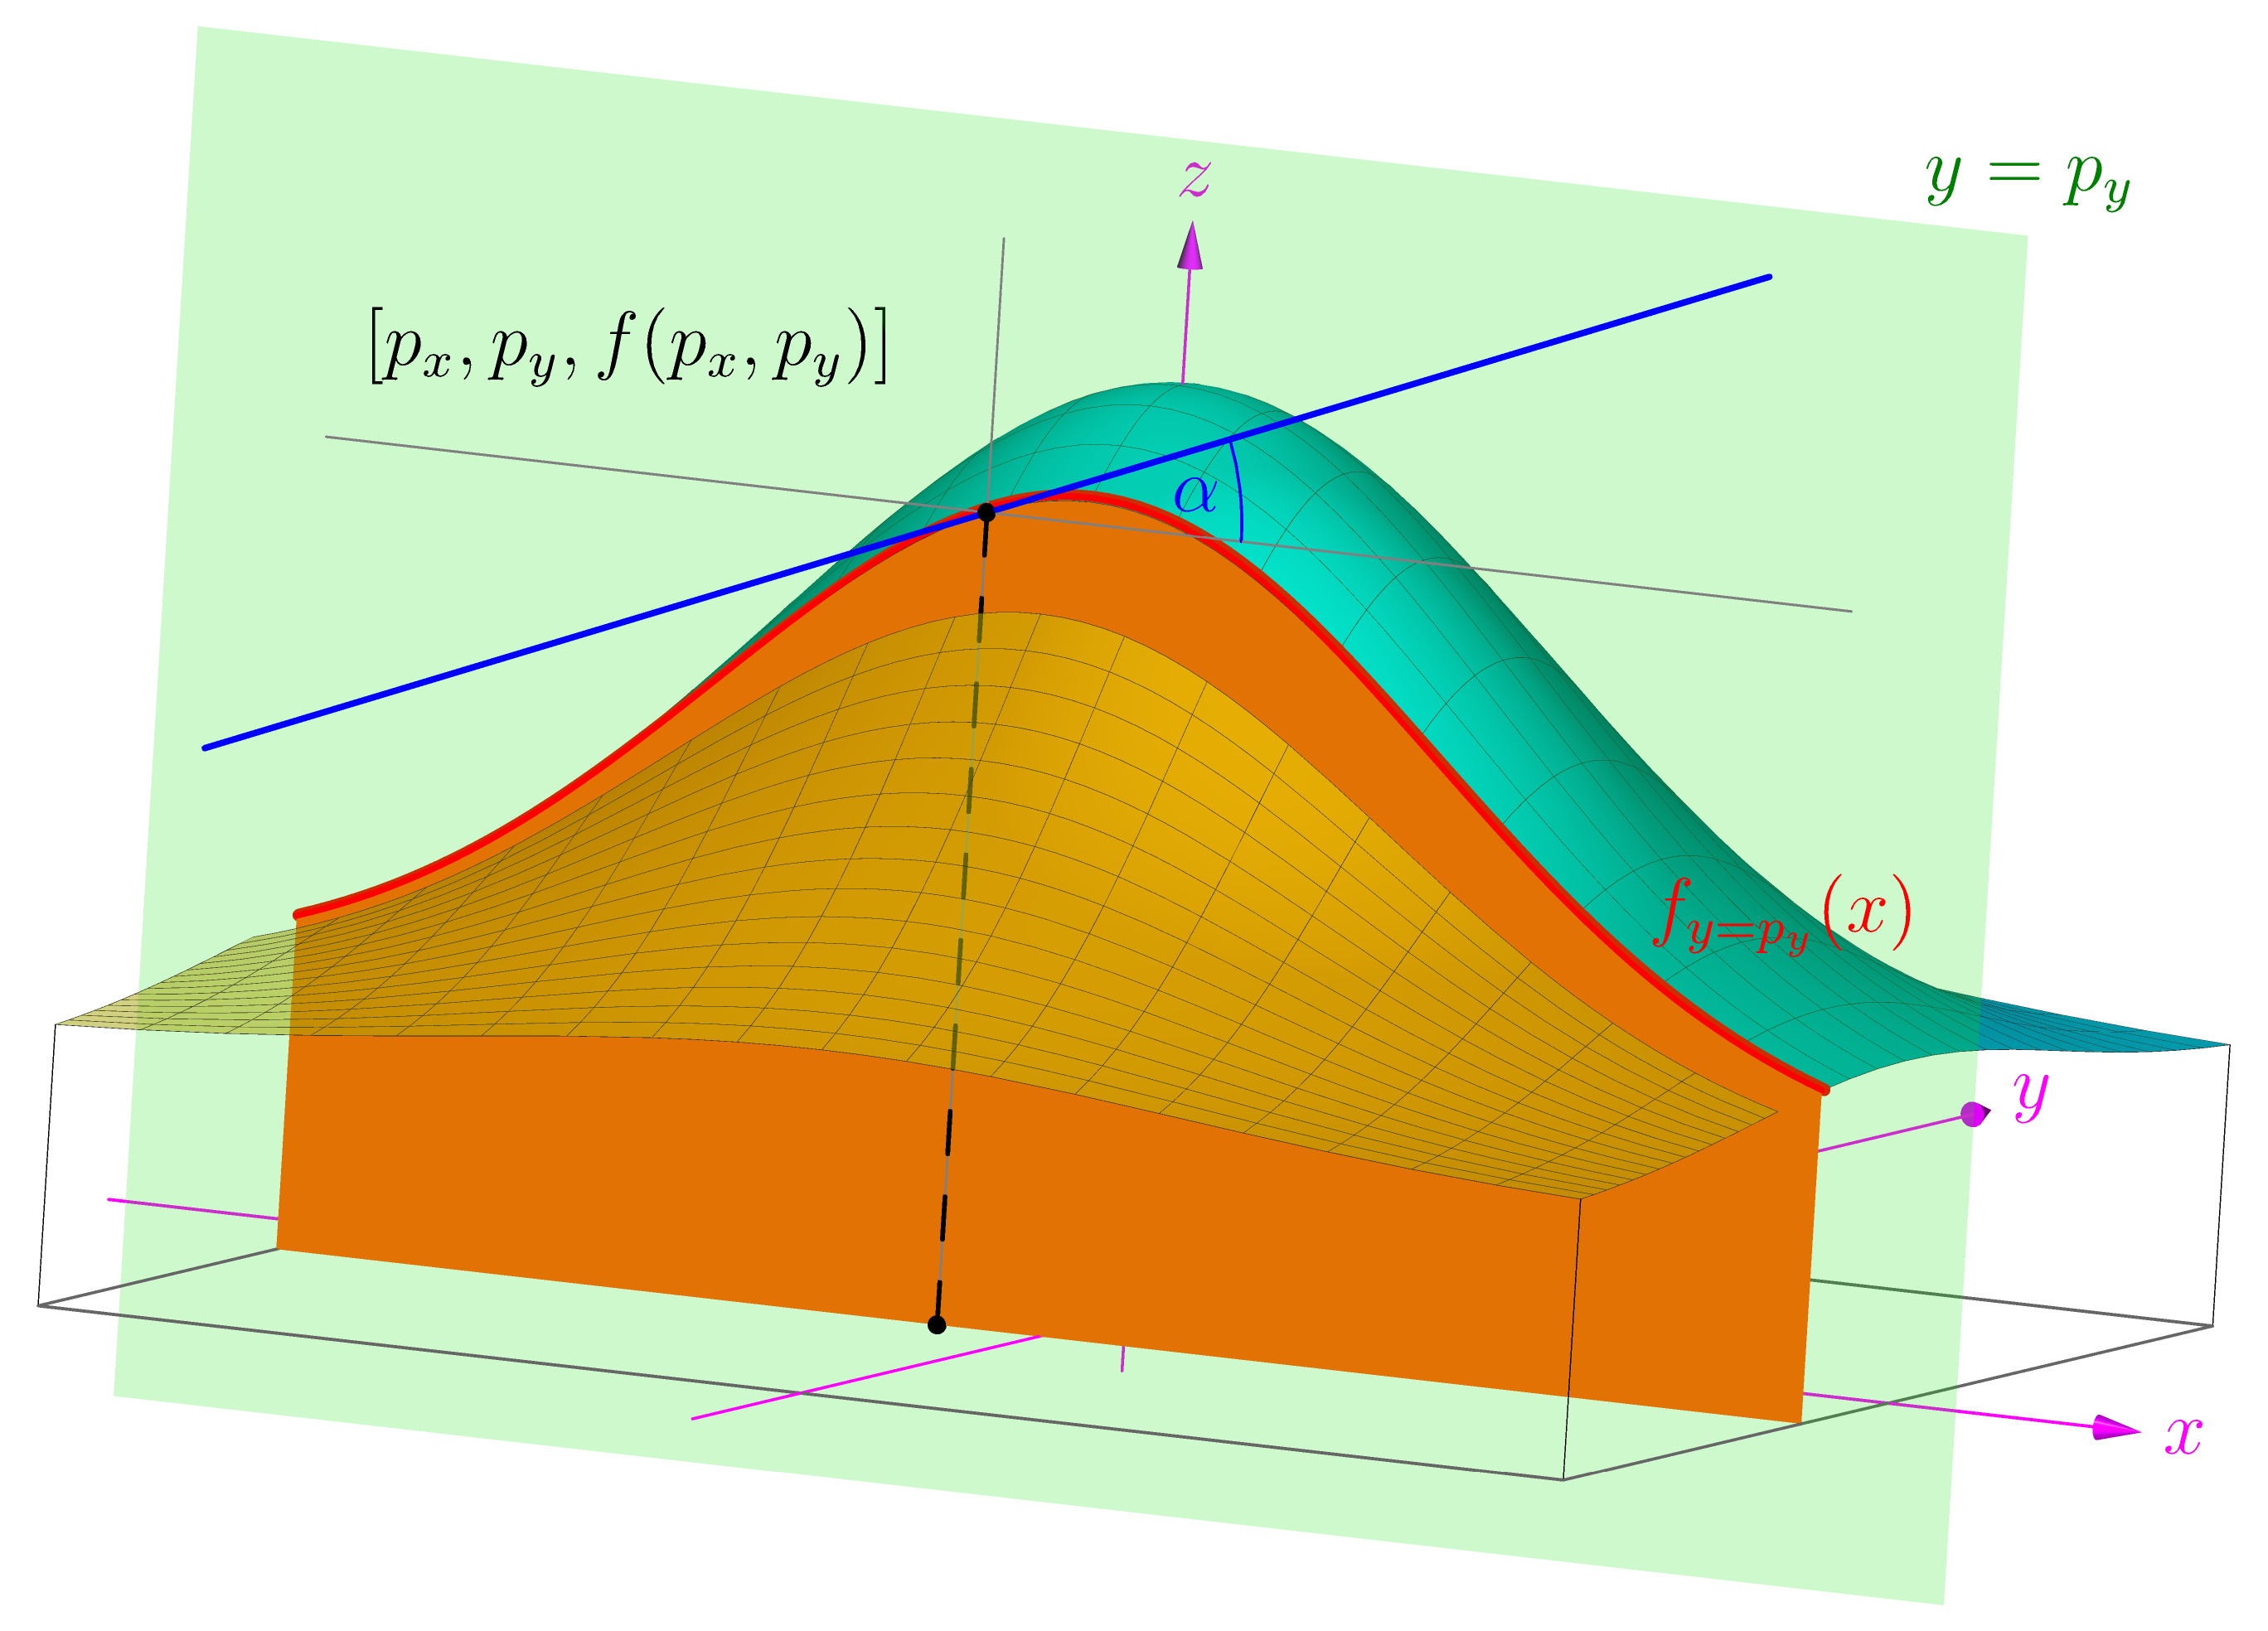
\includegraphics[width=12cm]{asy/partial1.png}}

Derivácia funkcie $f_{y=p_y}(x)$ v bode $p_x$ mi preto určuje, ako rastie výšková mapa
v bode $p$ v smere osi $x$. Toto je často používané číslo, preto  dostalo aj vlastný názov.\indexItem{Mat}{parciálna derivácia} 
Volá sa {\em parciálna derivácia} a zvykne sa označovať $\pdv{f}{x}(p)$.
To znamená, že keby som sa z bodu $p$ pohol o  veľmi malé $\Delta$ v smere 
osi $x$, tak hodnota $f(x,y)$ za zväčší o $\Delta\cdot\pdv{f}{x}(p)$.

Keď to podobne spravím pre os $y$, dostanem dva vektory $\vec{u}=\left[1,0,\pdv{f}{x}(p)\right]$ a  $\vec{v}=\left[0,1,\pdv{f}{y}(p)\right]$, ktoré mi určujú dotykovú rovinu
ku grafu funkcie $f$ v bode $\left[p_x,p_y,f(p_x,p_y)\right]$.

\centerline{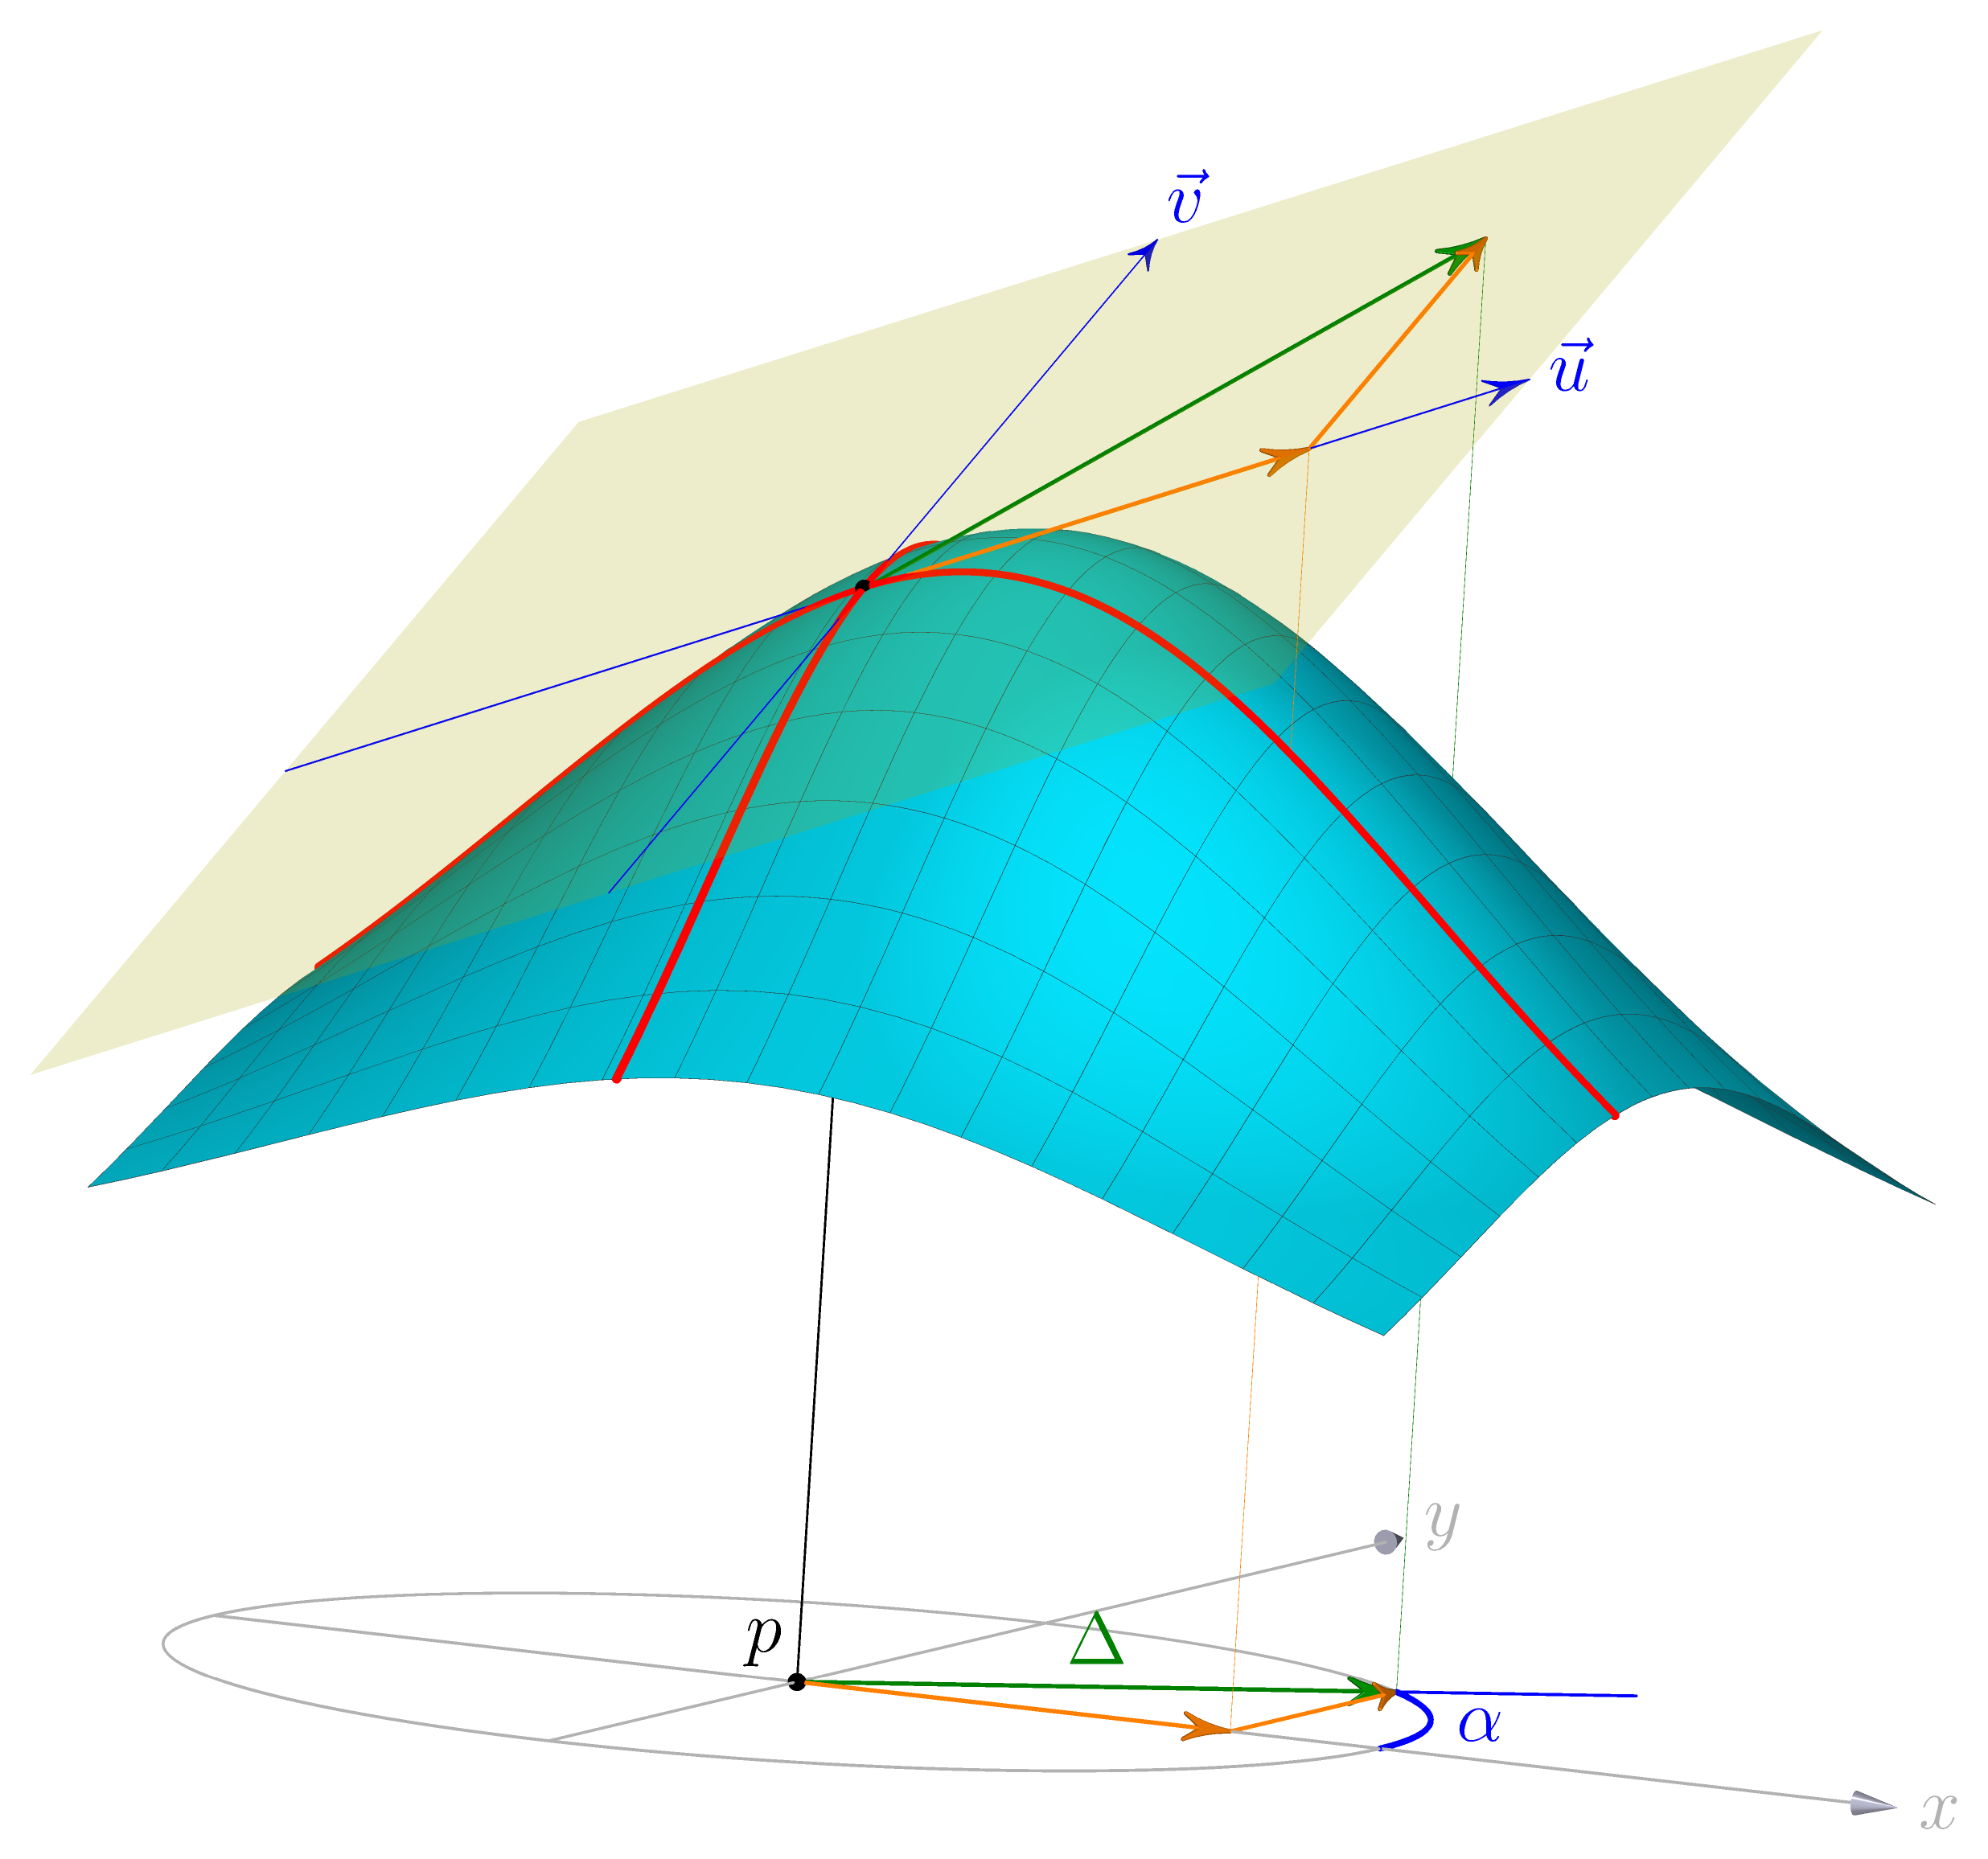
\includegraphics[width=11cm]{asy/partial2.png}}

Povedzme, že sa teraz pohnem z bodu $p$ o malý kúsok $\Delta$ pod uhlom $\alpha$. Zaujíma ma, ako sa zmení hodnota funkcie, ktorú si, ak je  $\Delta$ dosť malé, môžem nahradiť
dotykovou rovinou. Najprv sa pohnem v smere osi $x$ o $\Delta\cos(\alpha)$. Keďže v smere osi $x$ dotyková rovina rastie podľa vektora $\vec{u}$, 
hodnota narastie o $\Delta\cos(\alpha)\pdv{f}{x}(p_x,p_y)$. Potom sa pohnem v smere osi $y$ o $\Delta\sin(\alpha)$ a analogicky mi hodnota narastie o
$\Delta\sin(\alpha)\pdv{f}{x}(p_x,p_y)$. Keď to zrátam, dostanem, že keď som sa pohol o $\Delta$ pod uhlom $\alpha$, hodnota 
narástla o $\Delta\left(\cos(\alpha)\pdv{f}{x}(p_x,p_y)+\sin(\alpha)\pdv{f}{y}(p_x,p_y)\right)$.
Ak si označím $\vec{w}=\left[\cos(\alpha),\sin(\alpha)\right]$ vektor smeru o ktorý som sa pohol 
a $\vec\nabla=\left[\pdv{f}{x}(p_x,p_y),\pdv{f}{y}(p_x,p_y)\right]$ vektor parciálnych derivácií, vidím, že hodnota narástla o $\Delta(\vec{w}\cdot\vec{\nabla})$. A keď si pripomeniem,
čo sme rozprávali o skalárnom súčine na str.~\pageref{page:dotproduct-angle}, vidím, že hodnota narastie o
$\Delta\cdot\nrm{\vec{w}}\cdot\nrm{\vec{\nabla}}\cdot\cos(\varphi)$, kde $\varphi$ je uhol medzi vektormi $\vec{w}$ a $\vec{\nabla}$.

Akým smerom sa mám pohnúť, ak chcem, aby hodnota narástla čo najviac? Hodnoty $\Delta$, $\nrm{\vec{w}}$, $\nrm{\vec{\nabla}}$ sú stále rovnaké, jediné, čo sa mení, je
$\cos(\varphi)$. To znamená, že hodnota narastie najviac vtedy, keď $\cos(\varphi)$ bude $1$, t.j. keď $\varphi$ bude $0$. Inými slovami, hodnota narastie najviac
vtedy, keď sa pohnem v smere vektora $\vec{\nabla}$. 

Táto úvaha by sa dala zovšeobecniť aj na veľa rozmerov\footnote{To nie je úplne samozrejmé. Je veľa vecí, ktoré napr. platia v dvoch rozmeroch, ale v troch už nie (napr.
že dve priamky, ktoré nie sú rovnobežné, sa pretínajú), takže by bolo treba spraviť poriadny dôkaz pre veľa rozmerov. Tu ho ale neurobíme; išlo len o to ukázať intuíciu v pozadí.},
takže by sme dostali:


\begin{equation*}\boxed{\mathrm{Funkcia\ }n \mathrm{\ premenných\ } f(x_1,\ldots,x_n)
  \mathrm{\ rastie\ najrýchlejšie\ v\ smere\ vektora\ } gradientu \mathrm{\ }
\nabla=\left[\pdv{f}{x_1},\ldots,\pdv{f}{x_n}\right]}\end{equation*}

\vskip 1ex
Na záver matematickej odbočky si ešte raz všimni predchádzajúci obrázok. Máme tam funkciu $f(x,y)$
a jej dotykovú plochu v bode $p$. Čo by sa stalo, ak by $x$ a $y$ neboli premenné, ale 
nejaké funkcie parametra $t$, takže by nás zaujímala funkcia jednej premennej $h(t)=f(x(t),y(t))$?
Ako by vyzerala derivácia $\odv{h}{t}$? Ak parametrom $t$ pohnem o veľmi malé $\Delta$,
zmení sa hodnota $x(t)$ na  $x(t+\Delta)$. Keďže $\Delta$ je maličké, môžem si funkciu $x(t)$ nahradiť
jej dotyčnicou a dostanem $x(t+\Delta)\approx x(t)+\Delta\odv{x}{t}(t)$. Hodnota $y(t)$ sa podobne zmení na
$y(t+\Delta)\approx y(t)+\Delta\odv{y}{t}(t)$.
To znamená, že v dotykovej rovine k funkcii $f(x,y)$  
 sa pohnem o $\Delta\odv{x}{t}(t)$ v smere osi $x$ a hodnota funkcie
narastie o $\pdv{f}{x}(x(t),y(t))\Delta\odv{x}{t}(t)$. Potom sa pohnem 
o $\Delta\odv{y}{t}(t)$ v smere osi $y$ a hodnota funkcie narastie o ďalších $\pdv{f}{y}(x(t),y(t))\Delta\odv{y}{t}(t)$.
Dokopy teda ak pohnem parametrom $t$ o $\Delta$, hodnota $h(t)$ narastie o $\Delta\left(\pdv{f}{x}(x(t),y(t))\odv{x}{t}(t)+\pdv{f}{y}(x(t),y(t))\odv{y}{t}(t) \right)$.
Zasa by sa to dalo rozšíriť aj na viac rozmerov a dostali by sme analógiu derivácie zloženej funkcie pre viacero rozmerov:\indexItem{Mat}{derivácie zloženej funkcie vo viacerých rozmeroch}

\begin{equation*}\label{eq:diff_comp}\boxed{
    %\odv{f}{t}\left(g_1(t),g_2(t),\ldots,g_n(t)\right) = \sum_{i=1}^n\pdv{f}{g_i}\left(g_1(t),g_2(t),\ldots,g_n(t)\right)\cdot\odv{g_i}{t}(t)
    \begin{array}{c}
      \mathrm{Ak\ máme\ funkciu\ }f(x_1,\ldots,x_n) \mathrm{\ a\ } h(t)=f\left(g_1(t),g_2(t),\ldots,g_n(t)\right), \mathrm{\ potom\ }\\[1ex]
      \odv{h}{t}(t) = \sum\limits_{i=1}^n\pdv{f}{x_i}\left(g_1(t),\ldots,g_n(t)\right)\cdot\odv{g_i}{t}(t)
    \end{array}
}\end{equation*}


\def\err{\ensuremath{\mathrm{err}}}
\def\up#1{\ensuremath{^{(#1)}}}
\def\yh{\ensuremath{\widehat{\bm{Y}}}\xspace}
\vskip 2ex
Koniec matematickej odbočky, vráťme sa k našej jednoneurónovej ``sieti''. Povedali sme, že pre parametre $[w,b]$ je chyba siete $$\err(w,b)=\left(\tanh(wx_1+b)-y_1\right)^2.$$
Akým smerom treba pohnúť parametre, aby sa chyba čo najviac zmenšila? Teraz už vieme, že treba ísť v smere $-\nabla$, kde $\nabla$ je gradient
$\left[\pdv{\err}{w},\pdv{\err}{b}\right]$. Poďme teda rátať deriváciu. Funkciu $\tanh(\cdot)$ príliš nepoznáme, ale dá sa vyhľadať, že jej deriváciu už niekto zrátal a 
$$\tanh(x)'=\frac{1}{\cosh(x)^2}$$
$\cosh(\cdot)$ je nejaká iná funkcia, ktorá je dostupná z knižnice \vb{cmath} a to nám nateraz môže stačiť. Funkciu $\err$ si napíšeme ako zloženú funkciu takto

\begin{eqnarray*}
  \err(w,b) &=& \left(y(w,b)-y_1\right)^2\\
  y(w,b)&=&\tanh(u(w,b))\\
  u(w,b)&=&wx_1+b
\end{eqnarray*}

Použijeme, čo vieme o derivovaní zložených funkcií a napíšme si

\begin{align*}
  \pdv{\err}{w}=\pdv{\err}{y}\cdot\pdv{y}{u}\cdot\pdv{u}{w}& &
  \pdv{\err}{b}=\pdv{\err}{y}\cdot\pdv{y}{u}\cdot\pdv{u}{b}
\end{align*}

S tým, čo už vieme, zderivujeme jednotlivé funkcie ľahko:

\begin{align*}
  \pdv{\err}{y}=2(y-y_1)& &\pdv{y}{u}=\frac{1}{\cosh(u)^2}& &\pdv{u}{w}=x_1& &\pdv{u}{b}=1
\end{align*}

Keď to poskladáme dokopy, dostaneme

\begin{align*}
  \pdv{\err}{w}(w,b)=\frac{2x_1(\tanh(wx_1+b)-y_1)}{\cosh(wx_1+b)^2}& &
  \pdv{\err}{b}(w,b)=\frac{2(\tanh(wx_1+b)-y_1)}{\cosh(wx_1+b)^2}
\end{align*}

To znamená, že ak máme jednoneurónovú ``sieť'', tak pre akúkoľvek kombináciu 
$w$, $b$ vieme vyrátať, ktorým smerom treba hodnoty $w$ a $b$ pohnúť, aby sa chyba siete 
čo najrýchlejšie zmenšovala.


\vskip 1ex
Sieť s jedným neurónom nie je nič, čo by nás príliš uspokojilo, tak to poďme skúsiť zrátať 
pre zaujímavejšie siete. V našom programe máme triedu \vb{Network}, ktorá obsahuje pole vrstiev typu \vb{Layer}. 
Označme si vrstvy siete $L\up0,L\up1,\ldots,L\up{h-1}$. Každá vrstva obsahuje \vb{Matrix W,b}, tie vo vrstve $t$ si označme $\bm{W}\up{t}$, $\bm{b}\up{t}$.
Veľkosti vrstiev máme zapamätané vo \vb{vector<int> n}, takže $n_0$ je počet hodnôt na vstupe a $t$-ta vrstva $L\up{t}$ má $n_{t+1}$ neurónov,
takže $\bm{W}\up{t}$ je rozmerov $n_t\times n_{t+1}$ a $\bm{b}\up{t}$ je stĺpec $n_t\times1$. Tak, ako v predchádzajúcom hračkárskom príklade boli parametre siete
$w$ a $b$, teraz sú parametre všetky hodnoty vo všetkých
maticiach $\bm{W}\up{t}$, $\bm{b}\up{t}$. Podobne ako predtým, aj teraz potrebujeme zrátať chybu siete a potom gradient, t.j. deriváciu podľa každého z 
parametrov. Pripomeniem, že vyhodnocovanie vrstvy máme naprogramované takto:

\vskip 1ex
\vbox{
\begin{lstlisting}
Matrix Layer::eval(const Matrix &X) {
  Matrix res = W * X;
  res.addColumn(b);
  res.apply([](double x) { return tanh(x); });
  return res;
}
\end{lstlisting}}


Povedzme, že naša úloha má $s$ vstupov, takže vstupná matica $\bm{X}$ má rozmery $n_0\times s$. Prvá vrstva najprv 
vyráta $\bm{W}\up0\cdot\bm{X}$ a potom ku každému stĺpcu výsledku priráta $\bm{b}\up0$.
Tento medzivýsledok si označím $\bm{U}\up0$. Ak si označím $\bm{1}^s$ riadok obsahujúci $s$ jednotiek, ľahko sa overí, že $\bm{U}\up0=\bm{W}\up0\cdot\bm{X}+\bm{b}\up0\cdot\bm{1}^s$.
Nakoniec na každý prvok $\bm{U}\up0$ aplikujem $\tanh(\cdot)$. Túto operáciu budem označovať ako $\sigma\left(\bm{U}\up0\right)$ a výsledok označím $\bm{Y}\up0$.
Ak vstupom pre prvú vrstvu je vstupná matica $\bm{X}=\bm{X}\up0$, výstup z prvej vrstvy je vstupom pre druhú, t.j. $\bm{X}\up1=\bm{Y}\up0$.
Pri neurónových sieťach sa spravidla rozhodovacia funkcia neaplikuje na poslednú vrstvu, takže mám

\begin{align*}
  \bm{X}\up0&=\bm{X}\\
  \bm{U}\up{t}&=\bm{W}\up{t}\cdot\bm{X}\up{t}+\bm{b}\up{t}\cdot\bm{1}^s\\
  \bm{Y}\up{t}&=\sigma\left(\bm{U}\up{t}\right)\\
  \bm{X}\up{t+1}&=\bm{Y}\up{t}
\end{align*}


a dokopy sieť ráta zloženú funkciu

$$\bm{U}\up{h-1}=\bm{W}\up{h-1}\cdot\sigma\left(\bm{W}\up{h-2}\cdot\sigma\left(\cdots\sigma\left(\bm{W}\up0\cdot\bm{X}+\bm{b}\up0\cdot\bm{1}^s\right)\cdots\right)
+\bm{b}\up{h-2}\cdot\bm{1}^s\right)
+\bm{b}\up{h-1}\cdot\bm{1}^s$$


Ak si označím \yh maticu (rozmerov $h_{n-1}\times s$) správnych odpovedí, tak chyba siete, t.j. stredná kvadratická odchýlka, čiže priemer druhých mocnín rozdielov výstupných hodnôt a skutočných hodnôt, je


$$\err\left(\bm{W}\up0,\ldots,\bm{W}\up{h-1},\bm{b}\up0,\ldots,\bm{b}\up{h-1}\right)
=\frac{1}{s\cdot n_{h-1}}
\sum_{j=0}^{n_{h-1}}
\sum_{k=0}^{s-1}
\left(\yh_{j,k}-\bm{U}\up{h-1}_{j,k}\right)^2$$


$\err(\cdot)$ je veľmi zložitá funckia, v ktorej ako neznáme vystupujú všetky hodnoty z matíc $\bm{W}\up{t}$ a $\bm{b}\up{t}$. Aby sme zistili, ktorým smerom chyba najviac klesá, 
potrebujeme zrátať derivácie $\pdv{\err}{\bm{W}\up{t}_{j,k}}$ a $\pdv{\err}{\bm{b}\up{t}_j}$ pre všetky prípustné kombinácie $j$, $k$, $t$. 
Začneme s tým, že si pre všetky prípustné hodnoty $j$, $k$, $t$ vyrátame $\pdv{\err}{\bm{U}\up{t}_{j,k}}$.
\indexItem{Alg}{back propagation}
Pôjdeme pritom odzadu\footnote{preto sa táto metóda zvykne volať {\em back propagation}}. Pre fixné $j$, $k$ zrátame hodnotu $\pdv{\err}{\bm{U}\up{h-1}_{j,k}}$ tak,
že si predstavíme $\err$ ako funkciu jedinej premennej $\bm{U}\up{h-1}_{j,k}$ a zrátame deriváciu. Keď si rozpíšem zápis so sumami, dostanem

$$\err = \frac{1}{s\cdot n_{h-1}}\left(\yh_{0,0}-\bm{U}\up{h-1}_{0,0}\right)^2+\cdots+
 \frac{1}{s\cdot n_{h-1}}\left(\yh_{j,k}-\bm{U}\up{h-1}_{j,k}\right)^2+\cdots+
 \frac{1}{s\cdot n_{h-1}}\left(\yh_{n_{h-1},s-1}-\bm{U}\up{h-1}_{n_{h-1},s-1}\right)^2
$$

Už vieme, že derivácia konštantnej funkcie je $0$ a $\left(f(x)+g(x)\right)'=f'(x)+g'(x)$. V predchádzajúcom výraze je jediný člen, ktorý závisí od $\bm{U}\up{h-1}_{j,k}$, preto
všetko ostatné sa zderivuje na nulu a ostane mi

$$\pdv{\err}{\bm{U}\up{h-1}_{j,k}}=\frac{-2}{s\cdot n_{h-1}}\left(\yh_{j,k}-\bm{U}\up{h-1}_{j,k}\right)$$

Predstavme si teraz, že už máme pre nejaké $t$ zrátané $\pdv{\err}{\bm{U}\up{t+1}_{j,k}}$ pre všetky 
$j$, $k$ a chceme z nich vyrátať $\pdv{\err}{\bm{U}\up{t}_{j,k}}$.
Pretože $\bm{Y}\up{t}_{j,k}=\sigma\left(\bm{U}\up{t}_{j,k}\right)$ vždy aplikuje $\tanh(\cdot)$ na 
jednotlivé prvky v matici $\bm{U}$, predstavím si to ako zloženú funkciu a môžem si vyjadriť

$$\pdv{\err}{\bm{U}\up{t}_{j,k}}=
\pdv{\err}{\bm{Y}\up{t}_{j,k}}\cdot\odv{\bm{Y}\up{t}_{j,k}}{\bm{U}\up{t}_{j,k}}$$

pričom $\odv{\bm{Y}\up{t}_{j,k}}{\bm{U}\up{t}_{j,k}}$ je derivácia $\tanh(\cdot)$,
teda
$$ \odv{\bm{Y}\up{t}_{j,k}}{\bm{U}\up{t}_{j,k}}=\frac{1}{\cosh\left(\bm{U}\up{t}_{j,k}\right)^2}$$ 


Teraz chceme zrátať pre premennú $\bm{Y}\up{t}_{j,k}$ hodnotu $\pdv{\err}{\bm{Y}\up{t}_{j,k}}$, ak už máme zrátané všetky hodnoty $\pdv{\err}{\bm{U}\up{t+1}_{\ell,r}}$.
Na to použijeme rámček o zložených funkciách zo strany~\pageref{eq:diff_comp}: Najprv si predstavím, 
že $\err$ je funkcia premenných $\bm{U}\up{t+1}_{\ell,r}$
a potom si poviem, že v skutočnosti $\bm{U}\up{t+1}_{\ell,r}$ závisia od premenných $\bm{Y}\up{t}_{j,k}$, preto

$$\pdv{\err}{\bm{Y}\up{t}_{j,k}}=\sum_{\ell<n_{t+1}}\sum_{r<s}\pdv{\err}{\bm{U}\up{t+1}_{\ell,r}}\cdot\pdv{\bm{U}\up{t+1}_{\ell,r}}{\bm{Y}\up{t}_{j,k}}$$

Treba nám preto zistiť, ako závisí $\bm{U}\up{t+1}_{\ell,r}$ od $\bm{Y}\up{t}_{j,k}$.
Vieme, že $\bm{U}\up{t+1}=\bm{W}\up{t+1}\cdot\bm{Y}\up{t}+\bm{b}\up{t+1}\cdot\bm{1}^s$.
Keď si nakreslíme príslušné matice aj s ich rozmermi, bude to vyzerať takto:

\vskip 1ex
\centerline{
\begin{tikzpicture}
  \def\mtx#1[#2]#3[#4]#5{
    \draw(0,0) rectangle node{$#5$}(#2,#4);
    \draw[teal,draw=none](0,0) -- node[anchor=east]{$#3$}(0,#4);
    \draw[teal,draw=none](0,#4) -- node[anchor=south]{$#1$}(#2,#4);
  }

  \begin{scope}[shift={(-3,0)}]
    \mtx{s}[1.2]{n_{t+1}}[1.5]{\bm{U}\up{t+1}}
  \end{scope}
  
  \node at (-1.2,0.8) {$=$};


  \mtx{n_t}[2]{n_{t+1}}[1.5]{\bm{W}\up{t+1}}
  
  \node at (2.3,0.8) {$\cdot$};
  
  \begin{scope}[shift={(3,0)}]
    \mtx{s}[1.2]{n_t}[2]{\bm{Y}\up{t}}
  \end{scope}
  
  \node at (4.6,0.8) {$+$};
  
  \begin{scope}[shift={(5.4,0.4)}]
    \mtx{1}[0.4]{s}[1.2]{\bm{b}}
  \end{scope}
  \node at (6,0.8) {$\cdot$};
  \begin{scope}[shift={(6.5,0.4)}]
    \mtx{s}[1.2]{1}[0.4]{\bm{1}}
  \end{scope}

\end{tikzpicture}}

To znamená, že $$\bm{U}\up{t+1}_{\ell,r}=\sum_{i=0}^{n_t-1}\bm{W}\up{t+1}_{\ell,i}\bm{Y}\up{t}_{i,r}+\bm{b}\up{t+1}_\ell$$

Keďže nás zaujíma iba to, ako $\bm{U}\up{t+1}_{\ell,r}$ závisí od $\bm{Y}\up{t}_{j,k}$, vidíme, že ak $r\not=k$, tak $\bm{Y}\up{t}_{j,k}$ 
v tomto výraze nevystupuje a pre $r=k$ si môžeme  napísať

\def\oblacik{\raisebox{-0.6ex}{\usymH{1F5F0}{2.8ex}}\xspace}

$$\bm{U}\up{t+1}_{\ell,k}=\bm{W}\up{t+1}_{\ell,j}\bm{Y}\up{t}_{j,k}+\oblacik$$

pričom \oblacik od $\bm{Y}\up{t}_{j,k}$ nezávisí. Preto 
$\pdv{\bm{U}\up{t+1}_{\ell,k}}{\bm{Y}\up{t}_{j,k}}=\bm{W}\up{t+1}_{\ell,j}.$
Keď sa vrátime o krok späť, dostaneme

$$\pdv{\err}{\bm{Y}\up{t}_{j,k}}=\sum_{\ell<n_{t+1}}\pdv{\err}{\bm{U}\up{t+1}_{\ell,k}}\cdot\bm{W}\up{t+1}_{\ell,j}$$

\def\uh{\ensuremath{\widehat{\bm{U}}}\xspace}
\def\wh{\ensuremath{\widehat{\bm{W}}}\xspace}

Keď sa pozornejšie prizrieš, čo sme zrátali, pripomína to násobenie matíc. Ak si označím $\uh\up{t+1}$ maticu rozmerov $n_{t+1}\times s$, ktorá
bude obsahovať hodnoty $\pdv{\err}{\bm{U}\up{t+1}_{\ell,r}}$
a $\yh\up{t}$ maticu rozmerov $n_t\times s$, 
ktorá
bude obsahovať hodnoty $\pdv{\err}{\bm{Y}\up{t}_{j,k}}$, tak

$$\yh\up{t}=\bm{W}\tran{}\up{t+1}\cdot\uh\up{t+1}$$

Uff. Tak toto bolo trochu viac rátania, ale o to jednoduchšie budeme mať teraz programovanie. Triedu \vb{Layer} si prerobím tak, že si bude okrem matíc \vb{W} a \vb{b}
pamätať aj \vb{U}, \vb{Y} a \vb{dU}, čo budú naše matice $\bm{U}\up{t}$, $\bm{Y}\up{t}$ a $\uh\up{t}$.

\vskip 1ex
\vbox{
\begin{lstlisting}
struct Layer {
  int n1;       // počet neurónov vo vrstve
  int n0;       // veľkosť predchádzajúcej vrstvy (vstupu)
  Matrix W, b;  // W: n1 x n0, kde w[i,j] = váha i-teho neurónu k j-temu vstupu
                // b: stĺpec n1 x 1
  Matrix U, Y;  // n1 x s : výstupné hodnoty neurónov pred a po aktivácii
  Matrix dU;    // derivácia chyby podľa U
                
  Layer(int _n0, int _n1);   // konštruktor

  void feed(const Matrix&);                // spracuj vstup, nastav U
  void activate();                         // nastav Y podľa už nastaveného U
  void backPropagation(const Layer& nxt);  // nastav dU podľa nasledujúcej vrstvy
};
\end{lstlisting}
}



Jednotlivé metódy sa napíšu priamočiaro:

\vskip 1ex
\vbox{
\begin{lstlisting}
void Layer::feed(const Matrix &x) {
  if (x.m != s) {
    s = x.m;
    U = Matrix(n1, s);
  }
  multInto(W, x, U);
  U.addColumn(b);
}
\end{lstlisting}
}


\vskip 1ex
\vbox{
\begin{lstlisting}
void Layer::activate() {
  Y = U;
  Y.apply([](double x) { return tanh(x); });
}
\end{lstlisting}
}

\vskip 1ex
\vbox{
\begin{lstlisting}
void Layer::backPropagation(const Layer &nxt) {
  Matrix Z = (nxt.W.transposed()) * nxt.dU;
  dU = U;
  dU.apply([this](Num x) { 
      Num tmp = cosh(x);
      return 1.0 / (tmp * tmp);
  });
  dU.fill([this, &Z](int i, int j) { return dU(i, j) * Z(i, j); });
}
\end{lstlisting}
}


Metóda \vb{backPropagation} vyráta \vb{dU} v jednej vrstve na základe už vyrátanej \vb{dU} z nasledujúcej vrstvy.
Aby to celé mohlo odštartovať, potrebujeme zrátať \vb{dU} v poslednej vrstve. V nej rátame chybu pomocou \vb{mse},
takže si spravíme takúto funkciu, ktorá vyráta $\pdv{\err}{\bm{U}\up{h-1}_{j,k}}$ a výsledok uloží v matici \vb{D}:

\vskip 1ex
\vbox{
\begin{lstlisting}
void diffMse(const Matrix &data, const Matrix &truth, Matrix &D) {
    const int n = truth.n, m = truth.m;
    if (D.n != n || D.m != m) D = Matrix(n, m); // prerob ak nemá správne rozmery
    for (int i = 0; i < n; i++)
        for (int j = 0; j < m; j++)
            D(i, j) = -2.0 / (double)(n * m) * (truth(i, j) - data(i, j));
}
\end{lstlisting}
}

Celá sieť bude vstup spracovávať v metóde \vb{feed}, ktorá výsledok uloží v \hbox{\vb{layers[h - 1].U}}:

\vskip 1ex
\vbox{
\begin{lstlisting}
Matrix& Network::feed(const Matrix &input) {
  const Matrix *x = &input;
  for (int i = 0; i < h - 1; i++) {
    layers[i].feed(*x);
    layers[i].activate();
    x = &layers[i].Y;
  }
  layers[h - 1].feed(*x);
  return layers[h - 1].U;
}

Matrix& Matrix::output() { return layers[h - 1].U; }

Num Network::error(const Matrix &output, const Matrix &truth) { 
  return mse(output, truth); 
}
\end{lstlisting}
}

Volanie \vb{Network::backPropagation} najprv nechá vstupnú maticu prejsť vrstvu po vrstve 
cez celú sieť metódou \vb{feed}, ktorá v každej vrstve nastaví hodnoty \vb{U} a \vb{Y}. 
Potom v opačnom poradí nastaví v každej vrstve \vb{dU}. 

\vskip 1ex
\vbox{
\begin{lstlisting}
void Network::backPropagation(const Matrix &input, const Matrix &truth) {
  feed(input);
  diffMse(layers[h - 1].U, truth, layers[h - 1].dU);
  for (int i = h - 2; i >= 0; i--) layers[i].backPropagation(layers[i + 1]);
}
\end{lstlisting}
}


Stále ešte ale nemáme zrátaný gradient,
t.j. hodnoty $\pdv{\err}{\bm{W}\up{t}_{j,k}}$ a $\pdv{\err}{\bm{b}\up{t}_j}$.
Keď už ale máme zrátané $\pdv{\err}{\bm{U}\up{t}_{j,k}}$, tento zvyšok dorátame ľahko.
Vieme, že
$$\bm{U}\up{t}=\bm{W}\up{t}\cdot\bm{Y}\up{t-1}+\bm{b}\up{t}\cdot\bm{1}\up{s}$$
Pozrime sa najprv na tú ťažšiu vec, na $\pdv{\err}{\bm{W}\up{t}_{j,k}}$. Podobne, ako pred chvíľou,
predstavím si $\err$ ako zloženú funkciu premenných $\bm{U}\up{t}_{\ell,r}$, ktoré v skutočnosti závisia
od $\bm{W}\up{t}_{j,k}$ a dostanem
$$\pdv{\err}{\bm{W}\up{t}_{j,k}}=\sum_{\ell<n_t}\sum_{r<s}
\pdv{\err}{\bm{U}\up{t}_{\ell,r}}\cdot\pdv{\bm{U}\up{t}_{\ell,r}}{\bm{W}\up{t}_{j,k}}.$$

Pretože 
$$\bm{U}\up{t}_{\ell,r}=\sum_{i=0}^{n_t-1}\bm{W}\up{t}_{\ell,i}\bm{Y}\up{t-1}_{i,r}+\bm{b}\up{t}_\ell$$
tak viem, že $\bm{U}\up{t}_{\ell,r}$ závisí od môjho $\bm{W}\up{t}_{j,k}$
iba vtedy, keď $l=j$, a potom

$$\bm{U}\up{t}_{j,r}=\bm{W}\up{t}_{j,k}\bm{Y}\up{t-1}_{k,r}+\oblacik$$


$$\pdv{\err}{\bm{W}\up{t}_{j,k}}=
\sum_{r<s}\pdv{\err}{\bm{U}\up{t}_{j,r}}\cdot
\pdv{\bm{U}\up{t}_{j,r}}{\bm{W}\up{t}_{j,k}}=
\sum_{r<s}\pdv{\err}{\bm{U}\up{t}_{j,r}}\cdot
\bm{Y}\up{t-1}_{j,k}
$$


Opäť, ak si označím $\wh\up{t}$ maticu, kde budú hodnoty $\pdv{\err}{\bm{W}\up{t}_{j,k}}$,
tak 
$$ \wh\up{t}=\uh\up{t}\cdot\bm{Y}\bm\tran{}\up{t-1}$$

S hodnotami $\pdv{\err}{\bm{b}\up{t}_j}$ je to ešte jednoduchšie, lebo mám výraz

$$\pdv{\err}{\bm{b}\up{t}_{j}}=\sum_{\ell<n_t}\sum_{r<s}
\pdv{\err}{\bm{U}\up{t}_{\ell,r}}\cdot\pdv{\bm{U}\up{t}_{\ell,r}}{\bm{b}\up{t}_{j}}$$
a $\bm{U}\up{t}_{\ell,r}=\bm{b}\up{t}_\ell+\oblacik$.

Takže to môžeme rovno doprogramovať. Urobíme to tak, že potom, čo sa zavolá 
\hbox{\vb{Network::backPropagation()}} a nastavia sa \vb{dU} vo všetkých vrstvách, zavoláme 
\vb{Network::gradient()}, ktorý vyráta matice \vb{dW} a \vb{db} pre každú vrstvu.
Môžem si to spraviť tak, že každá vrstva vráti matice \vb{dW} a \vb{db}
v jednom type \vb{LayerData}. Pridané funkcie budú vyzerať nejak takto:

\vskip 1ex
\vbox{
\begin{lstlisting}
struct LayerData {
  Matrix dW, db;
};

using Gradient = std::vector<LayerData>;
\end{lstlisting}
}

\vskip 1ex
\vbox{
\begin{lstlisting}
LayerData Layer::gradient(const Matrix &Y) {
  LayerData res{dU * Y.transposed(), Matrix(n1, 1)};
  for (int j = 0; j < n1; j++) {
    res.db(j, 0) = 0;
    for (int k = 0; k < s; k++) res.db(j, 0) += dU(j, k);
  }
  return res;
}
\end{lstlisting}
}

\vskip 1ex
\vbox{
\begin{lstlisting}
Gradient Network::gradient(const Matrix &input) {
  Gradient res(h);
  for (int i = h - 1; i > 0; i--)
    res[i] = std::move(layers[i].gradient(layers[i - 1].Y));
  res[0] = std::move(layers[0].gradient(input));
  return res;
}
\end{lstlisting}
}

\vskip 1ex
\vbox{
\begin{lstlisting}
void Network::apply(Num a, const Network::Gradient &g) {
  for (int t = 0; t < h; t++) {
    layers[t].W.addMultiple(-a, g[t].dW);
    layers[t].b.addMultiple(-a, g[t].db);
  }
}
\end{lstlisting}
}

Pri trénovaní siete to potom vyzerá takto:

\vskip 1ex
\vbox{
\begin{lstlisting}
net.backPropagation(data, truth);
auto err = net.error(net.output(), truth);
auto g = net.gradient(data);
net.apply(step, g);
\end{lstlisting}
}

V riadku $2$ som si zrátal chybu, ktorú môžem použiť napríklad na to, aby som vedel, kedy s trénovaním prestať.
Parameter \vb{step} mi hovorí, koľko z gradientu mám prirátať, t.j. ako ďaleko sa v smere gradientu pohnem.
Zvoliť ho je celkom umenie: ak je príliš veľký, pôjdem v smere gradientu priďaleko a chyba siete narastie. Ak je 
príliš malý, trénovanie bude trvať pridlho. Môžeš si skúsiť rozmyslieť spôsob, ako \vb{step} automaticky meniť
(napr. ak chyba klesla, tak ho trochu zväčšiť, ak stúpla, tak ho zmenšiť).

\begin{uloha}
  Naprogramuj sieť, ktorá sa učí pomocou {\em back propagation} a otestuj ju
  na našom príklade s prvočíslami.
\end{uloha}


Keď som spúšťal túto vylepšenú sieť na príklade s 8-bitovými prvočíslami, kde 
náhodné učenie trvalo okolo 80000 iterácií, tak back propagation bolo spravidla veľmi rýchle, ale občas,
ak náhodné nastavenie siete na začiatku dopadlo nejak zle, učenie trvalo dlho. Preto som si povedal,
že ak sieť počíta viac ako 5000 iterácií a chyba je stále priveľká, sieť zahodím a skúsim to celé od začiatku. Vo výsledku mi stačilo v priemere 
4300 iterácií. To je oveľa menej, ako 80000 iterácií pri náhodnom učení, a pre väčšie siete by ten rozdiel bol ešte väčší.
Zároveň je vidieť, že čas stále dosť závisel od toho, ako sa na začiatku 
sieť náhodne nastavila.

\vskip 2ex
\newtoks\mycoords
\mycoords{}

\foreach \x[count=\i from 1] in {4347,	2605,	6875,	3398,	2148,	2484,	11775,	2271,	8771,	1589,
3800,	7184,	2090,	1525,	4532,	6852,	9574,	2967,	2352,	8491,	1492,	2299,	1386,
2270,	2159,	2283,	1457,	2510,	3262,	1935,	2743,	2942,	6819,	2515,	7495,	3858,
6532,	2170,	4869,	6920,	7581,	2394,	8506,	14079,	1805,	3558,	2756,	1523,	2468,
6641} {\global\mycoords\expandafter{%
  \expanded{\the\mycoords(\i,\x)}} }

\centerline{
\begin{tikzpicture}
  \begin{axis}[
      width=\textwidth, height=6cm, xmin=0, xmax=51, 
      ybar=0pt, bar width=2mm,  xtick=data, xticklabel=\empty,
       /pgf/number format/fixed,
       scaled y ticks=false,
      %1000 sep={}
   ]
    \addplot[ybar,fill=teal!50!white] coordinates {\the\mycoords};
  \end{axis}
\end{tikzpicture}}

\vskip 1ex
Doteraz sme sieť používali tak, že sme na nájdenie váh neurónov (a.k.a. {\em trénovanie}) použili všetky možné vstupy a výstupy úlohy. Čo ale s úlohami, ktoré majú 
priveľa možných vstupov? Urobíme to tak, že si vyberieme niekoľko vstupov a natrénujeme sieť iba na nich. Týmto nedostaneme presné riešenie úlohy, lebo o vstupoch, ktoré sme na
trénovanie nepoužili, nevieme nič. Môžeme sa ale spoliehať na to, že veľa úloh má takú vlastnosť, že vstupy, ktoré sú v istom zmysle podobné,
budú mať aj podobné riešenie. A rovnakú vlastnosť má aj neurónová sieť: na podobné vstupy dáva podobnú odpoveď. Ako dobre to môže fungovať závisí od konkrétnej úlohy. 
Poďme si to vyskúšať na jednoduchom príklade. Dajme tomu, že chcem mať sieť s dvoma vstupnými neurónmi, ktoré budú mať hodnoty medzi $-1$ a $1$. Tieto vstupné hodnoty sú súradnice
bodu v rovine a mojím cieľom je povedať, akú farbu má bod s danými súradnicami v tomto vzore:

\def\dim{2.5cm}
\vskip 1ex

{%
\setlength{\fboxsep}{0pt}%
\setlength{\fboxrule}{0.2pt}%
\centerline{\fbox{
\includegraphics[width=\dim]{data/netsamples/square2.png}}}
}

Zobral  som si  dve siete. Jedna mala tri vrstvy s 2, 5 a jedným neurónom a druhá štyri vrstvy s 2, 80,
80 a jedným neurónom. Potom som pre rôzne počty nádodne vybratých bodov natrénoval obe siete a
následne sa pozrel, aké odpovede dávali pre ostatné body.

\def\ms#1{%
{%
\setlength{\fboxsep}{0pt}%
\setlength{\fboxrule}{0.2pt}%
\raisebox{-1.25cm}{\fbox{\includegraphics[width=\dim]{data/netsamples/square2_2_5_1_sz0#1_dots.png}}}
}
}
\def\vs#1{%
{%
\setlength{\fboxsep}{0pt}%
\setlength{\fboxrule}{0.2pt}%
\raisebox{-1.25cm}{\fbox{\includegraphics[width=\dim]{data/netsamples/square2_2_80_80_1_sz0#1_dots.png}}}
}
}

\begin{column}{0.45}
\begin{tblr}{
  colspec = {Q[m,c]Q[m,c]Q[m,c]},
  stretch = 0,
  rowsep = 6pt,
  hline{1,Z} = {1pt},
  hline{2} = {0.5pt},
}
  vzorky& \vb{2,5,1} & \vb{2,80,80,1} \\
  10 & \ms{0010} & \vs{0010} \\
  40 & \ms{0040} & \vs{0040} \\
  60 & \ms{0060} & \vs{0060} \\
  100 & \ms{0100} & \vs{0100} \\
  150 & \ms{0150} & \vs{0150} \\
\end{tblr}
\end{column}
\hfill
\begin{column}{0.45}
\begin{tblr}{
  colspec = {Q[m,c]Q[m,c]Q[m,c]},
  stretch = 0,
  rowsep = 6pt,
  hline{1,Z} = {1pt},
  hline{2} = {0.5pt},
}
  vzorky& \vb{2,5,1} & \vb{2,80,80,1} \\
  200 & \ms{0200} & \vs{0200} \\
  300 & \ms{0300} & \vs{0300} \\
  400 & \ms{0400} & \vs{0400} \\
  600 & \ms{0600} & \vs{0600} \\
  1000 & \ms{1000} & \vs{1000} \\
\end{tblr}
\end{column}

Tu je dobre vidno, že malá sieť je príliš malá na to, aby sa vedela vzor naučiť, aj keď bolo na vstupe veľa bodov.
Veľká sieť ale už pri 200 vzorkách dáva celkom slušné výsledky. Takže ak máme šťastie a úloha, ktorú riešime, má
vhodnú štruktúru, môže nám stačiť pomerne málo testovacích príkladov na to, aby sa ju sieť naučila celkom rozumne riešiť.
Na druhej strane, to ``pomerne málo'' môže byť pre zložitejšie úlohy dosť veľa a nevieme ho dopredu poriadne odhadnúť.
Môžeme preto použiť nasledovný prístup: vyberieme si nejaký počet náhodných testovacích príkladov a urobíme niekoľko krokov 
back-propagation. Potom vyberieme iné náhodné príklady a zase na nich urobíme niekoľko krokov. V nasledujúcom experimente som 
si zobral tieto 4 vzory:

\vskip 2ex
\centerline{\includegraphics[width=0.9\textwidth]{data/evolution_pattern.png}}

Zobral som tri siete: prvá mala vrstvy \vb{2,25,1}, druhá \vb{2,100,20,1} a tretia \vb{2,850,150,10,1}. 
V jednej epoche som vybral 40 náhodných bodov a spravil 200 iterácií back-propagation.
Po 900 epochách to vyzeralo takto:

\vskip 2ex
\centerline{\includegraphics[width=0.9\textwidth]{data/frame00900.png}}

\begin{uloha}
Pozri si \link{\rootpath/evolution.mp4}{video} z predchádzajúceho experimentu. Čo sa z neho dá vidieť? 
Naprogramuj podobný experiment.  
Ako by sa dalo trénovanie urýchliť lepšou voľbou parametrov (veľkosť siete, veľkosť vzorky, dĺžka 
  epochy)?
\end{uloha}

\section*{Projekt: rozpoznávanie písaných číslic}
\label{projekt.cislice}
\setlength{\fboxsep}{0pt}%
\setlength{\fboxrule}{0.2pt}%

Výsledkom tohoto projektu bude program, v ktorom môžeš myšou nakresliť číslicu, program ju rozpozná a zasvieti príslušné číslo. Vyzerať by to
malo nejak takto\footnote{Výsledný program si môžeš vyskúšať tu: \href{https://beda.dcs.fmph.uniba.sk/mnist/digits.html}{\nolinkurl{https://beda.dcs.fmph.uniba.sk/mnist/digits.html}}}:

\vskip 2ex
\centerline{
  \includegraphics[width=0.45\textwidth]{data/mnist_app.png}
%  \hfill
%  \includegraphics[width=0.45\textwidth]{data/mnist_app2.png}
}

Namiesto toho, aby som sa snažil naprogramovať tvary jednotlivých číslic, natrénujem na rozpoznávanie neurónovú sieť: každý pixel zo vstupu bude jeden vstupný neurón s hodnotou od
$-1$ pre 
bielu po $1$ pre čiernu. Na 
výstupnej vrstve bude 10 neurónov a každý bude reprezentovať jednu číslicu (čím väčšia hodnota neurónu, tým viac si sieť myslí, že je na vstupe daná číslica).
Aby som sieť mohol trénovať, potrebujem veľa príkladov napísaných číslic. Americký NIST (National Institute of Standards and Technology) má verejnú
\link{https://www.nist.gov/srd/nist-special-database-19}{databázu} rukou písaných písmen a číslic, ktorá sa dá použiť. Tá časť, čo ma zaujíma, sú rukou písané číslice,
každá je čierno-biely obrázok rozmerov $128\times128$ vo formáte png, napr:

\fbox{\includegraphics[width=2cm]{data/mnist_2.png}}
\hfill
\fbox{\includegraphics[width=2cm]{data/mnist_8.png}}
\hfill
\fbox{\includegraphics[width=2cm]{data/mnist_2b.png}}
\hfill
\fbox{\includegraphics[width=2cm]{data/mnist_4.png}}
\hfill
\fbox{\includegraphics[width=2cm]{data/mnist_9.png}}
\hfill
\fbox{\includegraphics[width=2cm]{data/mnist_3.png}}

\vskip 1ex
Na použitie v neurónovej sieti si ich potrebujem pripraviť. Jednak mať $128\times128=16384$ vstupných neurónov by bolo priveľa a jednak by sieť bola citlivá na posunutie. Napr.
tieto dve verzie dvojky sú takmer rovnaké, ale aktivované by boli úplne rôzne vstupné neuróny:

\vskip 2ex
\centerline{\fbox{\includegraphics[width=4cm]{data/mnist_shift.png}}}


Povedal som si, že mi bude stačiť $26\times26=676$ vstupných neurónov. 
Predspracovanie obrázka robím takto: zistím si bounding box, t.j. najmenší obdĺžnik, v ktorom sú všetky
čierne pixely. Potom ho upravím na štvorec podľa dlhšej strany:

\vskip 2ex
\centerline{\fbox{\includegraphics[width=4cm]{data/mnist_2bbox.png}}}

Štvorec vyrežem, zmenším na rozmer $18\times18$ a nájdem ťažisko čiernych (sivých) pixelov:

\vskip 3ex
\centerline{\fbox{%
\begin{tikzpicture}[scale=0.35]
  \foreach \l[count=\i] in {%
{ 255, 255, 255, 255, 255, 255, 255, 255, 255, 255, 255, 255, 255, 255, 255, 252, 251, 255 },
{ 255, 255, 255, 253, 254, 255, 255, 255, 255, 255, 255, 255, 255, 254, 252, 255, 255, 255 },
{ 255, 255, 254, 255, 255, 251, 254, 255, 255, 255, 255, 255, 253, 255, 255, 186, 128, 254 },
{ 255, 254, 255, 230, 248, 255, 255, 254, 255, 255, 255, 254, 255, 254, 99, 0, 0, 237 },
{ 251, 255, 151, 0, 40, 89, 231, 255, 254, 255, 255, 253, 255, 76, 0, 0, 99, 255 },
{ 255, 190, 0, 0, 0, 0, 150, 255, 251, 255, 251, 255, 132, 0, 3, 11, 239, 255 },
{ 255, 18, 0, 3, 71, 0, 148, 255, 251, 253, 255, 221, 13, 0, 0, 166, 255, 252 },
{ 95, 0, 20, 174, 255, 91, 155, 255, 252, 249, 255, 120, 0, 0, 94, 255, 252, 255 },
{ 0, 13, 216, 255, 251, 255, 252, 255, 252, 255, 255, 46, 0, 6, 240, 255, 247, 254 },
{ 56, 0, 185, 255, 249, 253, 255, 249, 255, 251, 73, 0, 0, 0, 85, 206, 255, 255 },
{ 177, 0, 35, 250, 255, 250, 255, 255, 240, 45, 0, 99, 156, 6, 0, 14, 93, 223 },
{ 255, 73, 0, 86, 255, 255, 248, 153, 21, 0, 155, 255, 255, 215, 150, 12, 0, 33 },
{ 255, 245, 79, 0, 36, 60, 15, 0, 42, 207, 255, 253, 250, 255, 255, 246, 99, 0 },
{ 253, 255, 255, 99, 2, 0, 42, 173, 255, 255, 250, 255, 255, 252, 250, 255, 34, 125 },
{ 255, 253, 255, 255, 237, 233, 255, 255, 254, 252, 255, 255, 255, 251, 255, 148, 0, 246 },
{ 255, 255, 254, 252, 255, 255, 255, 251, 254, 255, 255, 255, 254, 255, 255, 72, 184, 255 },
{ 255, 255, 255, 255, 253, 253, 254, 255, 255, 255, 255, 255, 255, 255, 252, 253, 255, 254 },
{ 255, 255, 255, 255, 255, 255, 255, 255, 255, 255, 255, 255, 255, 255, 255, 255, 253, 255 }} {
    \foreach \v[count=\j] in \l {
      \fill[fill={rgb,255:red,\v; green,\v; blue,\v}] (\i,-\j) rectangle ++(0.9,0.9);
    }
  }

  \fill[red](8,-8) rectangle ++(0.9,0.9);
\end{tikzpicture}}}

Napokon výsledok vycentrujem tak, aby ťažisko bolo v strede štvorca $26\times26$.
Týmto spôsobom dostanem všetky číslice rovnako veľké a rovnako umiestnené. Ak budem tým 
istým spôsobom spracovávať aj nakreslené vzory v programe, nebudem mať problémy s rôzne veľkými a 
rôzne posunutými číslami. Výsledok spracovania niektorých čísel z trénovacieho datasetu vyzerá  takto (všimni si drobné
rozdiely v typickom písaní niektorých číslic oproti Slovensku):


\vskip 2ex
\centerline{\includegraphics[width=\textwidth]{data/mnist.png}}

Vieme, čo chceme dosiahnuť, tak to môžeme začať programovať. Najprv si spravím pomocné triedy pre pixel a obdĺžnik

\vbox{\begin{lstlisting}
struct Point {
  int _p[2];
  Point &operator=(const Point &a);
  int &x() { return _p[0]; }
  int &y() { return _p[1]; }
  int x() const { return _p[0]; }
  int y() const { return _p[1]; }
  int &operator[](int i) { return _p[i]; }
  int operator[](int i) const { return _p[i]; }
  Point &operator+=(const Point &p);
  Point &operator*=(double a);
};
\end{lstlisting}}

\vbox{\begin{lstlisting}
struct Box {
  Point p[2];   // ľavý horný a pravý dolný okraj
  Point &operator[](int i) { return p[i]; }
  Point operator[](int i) const { return p[i]; }
  int x() const { return p[1].x() - p[0].x(); }
  int y() const { return p[1].y() - p[0].y(); }
  Box &expand(const Point &q); // rozšír obdĺžnik tak, aby obsahoval bod q
  Point center() const;
};
\end{lstlisting}}

Doprogramovať zvyšné metódy by malo byť priamočiare. Ďalej si urobím pomocnú triedu na uloženie
štvorcového obrázka rozmerov $d\times d$:

\vskip 2ex
\vbox{\begin{lstlisting}
using u8 = uint8_t;

struct Bytes {
  std::vector<u8> a;
  int d, n;
  u8 sentinel;
  Bytes(int _d) : d{_d}, n{d * d} { 
    a.resize(n, 255); // miesto na štvorec d x d, celý biely
  }
  u8 &operator()(int x, int y);
  u8 operator()(int x, int y) const;
  Point pos(int i) const { 
    return Point{i % d, i / d}; // súradnice i-teho pixelu
  }
  Point cog() const; // ťažisko
  Box bbox() const;  // bounding box
};
\end{lstlisting}}

Premennú \vb{sentinel} som použil na to, aby som mohol kontrolovať, či parametre v \vb{operator()}
nie sú mimo rozsahu. Keďže vraciam referenciu, potrebujem vrátiť niečo, kam sa dá beztrestne zapisovať.

\vskip 2ex
\vbox{\begin{lstlisting}
u8 &Bytes::operator()(int x, int y) {
  if (x < 0 || y < 0 || x >= d || y >= d) return sentinel;
  return a[x + y * d];
}
\end{lstlisting}}

Nájsť bounding box je jednoduché

\vskip 2ex
\vbox{\begin{lstlisting}
Box Bytes::bbox() const {
  Box b{Point{n, n}, Point{0, 0}};
  for (int i = 0; i < n; i++)
    if (a[i] < 255) b.expand(pos(i));
  return b;
}
\end{lstlisting}}

Ďalej budem potrebovať výrez naškálovať na rozmer $18\times18$. Aj keď sa to nezdá, škálovanie je celkom zložitý problém, ak ho chceš spraviť poriadne. Ak by som 
chcel iba napr. zmenšiť obrázok na polovicu, tak jednému pixelu výsledného obrázka prislúchajú štyri pixely (štovrec $2\times2$) z pôvodného. Stačí mi preto spraviť
priemer z tých štyroch a je to. Ak ale rozmer nového ovrázka nie je deliteľom pôvodného, začnú problémy. Pre naše účely to nie je zase také dôležité, ale rozhodol som sa
spraviť výnimku a použiť externú knižnicu, konkrétne škálovaciu knižnicu 
\link{https://github.com/avaneev/avir}{Avir}. Používa sa ľahko. Keďže všetko v nej je šablóna, stačí nakopírovať súbor
\link{https://github.com/avaneev/avir/raw/master/avir.h}{avir.h} do pracovného adresára a použiť \prg~#include "avir.h"~.
Potom môžeš vyrobiť premennú typu\footnote{\indexItem{Prg}{šablóny s default parametrami}tie prázdne zátvorky \prg~<>~ znamenajú, že \prg~CImageResizer~ je šablóna s default parametrom, podobne, ako keď majú
default parametre funkcie. Konkrétne \prg~avir::CImageResizer<>~ je to isté ako \prg~avir::CImageResizer< avir::fpclass_def<float> >~} \prg~avir::CImageResizer<>~. Konštruktor dostane ako parameter počet bitov na farbu, v našom prípade $8$.
Celú prácu potom urobí metóda \prg~resizeImage~

\vskip 2ex
\vbox{\begin{lstlisting}
avir::CImageResizer<>::resizeImage(
    const u8 *src,                     // pointer na dáta pôvodného obrázka
    const int src_w, consit int src_h, // rozmery pôvodného obrázka
    int lineSize,                      // veľkosť riadka, môže vždy ostať 0
    u8 *dst,                           // pointer na dáta výsledného obrázka
    const int dst_w, const int dst_h,  // výsledné rozmery
    const int numChan,                 // počet kanálov na pixel, pre nás 1 
                                       // (napr. pre RGB by bolo 3, pre RGBA 4)
    const double k                     // krok algoritmu, tu vždy môže ostať 0
  );
\end{lstlisting}}

Posledná vec, ktorú potrebujem, je nájsť ťažisko. To spravím tak, že zrátam vážený priemer pixelov (biely má váhu 0, čierny váhu 255):

\vskip 2ex
\vbox{\begin{lstlisting}
Point Bytes::cog() const {
  Point p{0, 0};
  int s = 0;
  for (int i = 0; i < d * d; i++) {
    u8 v = 255 - a[i];
    Point q = v * pos(i);
    s += v;
    p += q;
  }
  for (int i = 0; i < 2; i++) 
    p[i] = (int)((double)(p[i]) / (double)s);
  return p;
}
\end{lstlisting}}

Celá funkcia na spracovanie obrázku vyzerá takto:

\vskip 2ex
\vbox{\begin{lstlisting}
void processImage(Bytes &in, Bytes &out) {
  Box bb = in.bbox();
  int d = 1 + max(bb.x(), bb.y());  // dlhšia strana bounding boxu

  // o je ľavý horný pixel vyrezaného štvorca
  Point o{bb[0].x() - (d - bb.x()) / 2, bb[0].y() - (d - bb.y()) / 2};
  Bytes crop(d);  // sem uložím vyrezaný štvorec d x d
  int t = 0;
  for (int i = 0; i < d; i++)
    for (int j = 0; j < d; j++) {
      in.sentinel = 255;  // ak som mimo rozsahu, prečítam bielu
      crop.a[t++] = in(o.x() + j, o.y() + i);
    }

  Bytes rsz(sc); // sem uložím naškálovaný výsledok
  imageResizer.resizeImage(crop.a.data(), d, d, 0, rsz.a.data(), sc, sc, 1, 0);

  Point c = rsz.cog(); // ťažisko
  o = Point{dim / 2 - c.x(), dim / 2 - c.y() - 1}; // okraj vycentrovaného štvorca

  for (int i = 0; i < sc; i++)
    for (int j = 0; j < sc; j++)
        out(o.x() + j, o.y() + i) = rsz(j, i);
}

\end{lstlisting}}

Takto som spracoval celý dataset. Výsledok je v súbore
\link{\rootpath/mnist.zip}{mnist.zip} kde je pre každú číslicu jeden dlhý binárny súbor. V ňom je najprv počet obrázkov ako 32-bitový integer a za ním
idú jednotlivé $26\times26$ obrázky za sebou jeden byte na každý pixel, takže
prečítať to viem takto:

\vskip 2ex
\vbox{\begin{lstlisting}
vector<vector<Bytes>> dataset(10); // pre každú číslicu je zoznam obrázkov

for (int num = 0; num < 10; num++) {
  stringstream ss;
  ss << "./mnist/" << num << ".bin";
  ifstream f(ss.str(), ios::binary);
  uint32_t x;
  f.read((char *)&x, 4);  // prečítam 32 bitov (4 byty) počet obrázkov
  while (x-- > 0) dataset[num].emplace_back(dim); // vyrobím miesto pre obrázky
  for (auto &d : dataset[num]) 
      f.read((char *)(d.a.data()),  dim * dim);   // postupne všetky prečítam
}
\end{lstlisting}}

\begin{uloha}
  Natrénuj neurónovú sieť na datasete číslic. Do triedy \vb{Network} pridaj metódy \vb{save} a \vb{load} a natrénovanú sieť ulož do súboru.
\end{uloha}

Ja som použil sieť s vrstvami so \vb{676,300,100,10} neurónmi a trénoval som po epochách 1000 iterácií vždy na vzorke 200 náhodne vybratých číslic.

\vskip 4ex
Keď už je natrénovaná sieť uložená v súbore, ostáva spraviť program, ktorý ju používa a v ktorom sa
dajú kresliť číslice. Na to sa dajú použiť widgety z kapitoly~\ref{sect:dedicnost}. 
Hlavné okno bude \vb{VLayout mainWindow}, v ktorom budú dva \vb{HLayout}y: \vb{topBar}
a \vb{mainArea}. V \vb{topBar}
desať widgetov typu \vb{Bulb}, ktoré zobrazujú jednotlivé číslice. V \vb{mainArea}
bude vľavo widget typu \vb{Canvas}, ktorý sa stará o kreslenie a vpravo \vb{VLayout buttonArea} 
s gombíkmi:

\vskip 2ex
\vbox{\begin{lstlisting}
Canvas *canvas = nullptr;
Bulb *bulbs[10];
...

int main() {
  ...
  VLayout mainWindow;
  canvas = new Canvas();
  auto topBar = new HLayout();
  topBar->fixedHeight = 52;
  auto mainArea = new HLayout();
  auto buttonArea = new VLayout();
  buttonArea->fixedWidth = 150;
  Button *quitButton = new Button("koniec");
  Button *clearButton = new Button("znovu");

  for (int i = 0; i < 10; i++) {
    bulbs[i] = new Bulb(to_string(i));
    (*topBar) << bulbs[i];
  }

  mainWindow << topBar << mainArea;
  (*mainArea) << canvas << buttonArea;
  (*buttonArea) << new Widget() << clearButton << quitButton;

  ...
}
\end{lstlisting}}

Widget \vb{Bulb} môžeme spraviť modifikáciou \vb{Button}: bude vždy disabled, aby sa naňho
nedalo klikať. Navyše bude mať metódu \vb{set(double d)}, ktorá nastaví pozadie od
červenej po zelenú. Na to môžem použiť \vb{Gradient} z úlohy~\ref{uloha:gradient}.

\vskip 2ex
\vbox{\begin{lstlisting}
struct Bulb : Button {
  static const Gradient g;
  Bulb(const std::string &_txt) ;
  void set(double val) ;
};

const Gradient Bulb::g("gradient.gpf");
\end{lstlisting}}

Nakoniec treba dorobiť triedu \vb{Canvas}. V nej budem mať \vb{Bytes img} pre obrázok 
(napr. $70\times70$), v metóde i\hbox{\vb{render}} ho vykreslím zo štvorčekov. Zároveň budem
v metódach \vb{onMouseDown} a \vb{onMouseUp} sledovať polohu myši a kresliť. Keďže
myš sa môže pohybovať dosť rýchlo, je lepšie vždy vykresliť čiaru od posledného zapamätaného
miesta po súčasné. Na to môžem použiť algoritmus kreslenia čiary z úlohy~\ref{uloha:editor}.

\vskip 2ex
%\vbox{
\begin{lstlisting}
struct Canvas : Widget {
  const int dim = 70;
  int pxdim, spacing;  // rozmer štvorčeka a medzeru medzi nimi
                       // si budem nastavovať v resize
  Bytes img;
  bool painting;       // či je stlačený gombík myši
  SDL_Point lastMouse; // posledná poloha myši, odtiaľ kreslím čiaru

  Canvas();             // konštruktor
  ~Canvas();

  void clear();
  void line(SDL_Point,SDL_Point); // vykresli čiaru
  void resize(SDL_Rect scr);      // nastaví všetko potrebné pri zmene okna
  void render(SDL_Renderer *renderer);

  void onMouseDown(SDL_MouseButtonEvent& e);
  void onMouseUp(SDL_MouseButtonEvent& e);

  ... // pomocné metódy
};
\end{lstlisting}
%}

V hlavnom programe v pravidelných intervaloch spustím sieť na aktuálnom vstupe:

\vskip 2ex
\vbox{\begin{lstlisting}
void run_net() {
  auto &inp = canvas->img;     // nakreslený obrázok
  Matrix in(dim * dim, 1);     // vstup pre sieť

  Bytes tmp(inp.d);            // pred zmenšením  vstup 
                               // trochu rozmažem
  int d = inp.d;
  inp.sentinel = 255;
  for (int i = 0; i < d; i++)
    for (int j = 0; j < d; j++) {
      int v = 0;
      for (int di : {-1, 0, 1})
        for (int dj : {-1, 0, 1}) v += inp(i + di, j + dj);
      tmp(i, j) = u8(v / 9);
    }

  Bytes img(26);
  processImage(tmp, img);      // zmenši a vycentruj

  // vyrob vstup pre sieť a spusti ju
  for (int i = 0; i < 26 * 26; i++)
    in(i, 0) = 1.0 - 2.0 * (double)img.a[i] / 255.0;
  auto &out = net.feed(res.in);

  // nastav farby podľa výsledku
  for (int i = 0; i < 10; i++) bulbs[i]->set(tanh(out(i, 0)));
}
\end{lstlisting}}

\begin{uloha}
  Naprogramuj GUI tak, aby zyeralo ako screenshot na začiatku kapitoly.
\end{uloha}

\newpage
\phantom{aa}
\vfill
... a to je nateraz všetko. Je veľa vecí, o ktorých som tu nerozprával, ale raz skončiť treba.
Ako stručná odpoveď na otázku \cmd{``Ako sa programuje v C++''} to snáď stačí.

\centerline{\usymH{1F514}{2.5cm}}



\immediate\closeout\indexFile


\chapter{Kde je čo}
\tikzexternaldisable

\def\itemLineClr{\AlgColor}
\def\itemLine#1#2{%

\noindent
\hspace*{3mm}\textcolor{\itemLineClr}{\roboto #1}\dotfill\hyperref[#2]{\pageref{#2}}}

Programátorské projekty s otvoreným koncom, s ktorými sa dá hrať ďalej:

\itemLine{Celulárny automat}{projekt.automat}
\itemLine{Offline grafický editor}{sect:editor}
\itemLine{Mandelbrotova množina}{projekt.mandelbrot}
\itemLine{Kompresia textu}{projekt.pakovac}
\itemLine{Mapy náhodných ostrovov}{sect:ostrovy}
\itemLine{Hra \btr}{projekt.breakthrough}
\itemLine{Rozpoznávanie číslic}{projekt.cislice}


\vskip 2ex
\def\itemLineClr{\MatColor}
Matematické odbočky:

\itemLine{Pytagorova veta, Euklidova vzdialenosť a kruhy}{mat.pytagoras}
\itemLine{Goniometrické funkcie $\sin$ a $\cos$}{sect:sin_cos}
\itemLine{Komplexné čísla}{mat.komplex}
\itemLine{Body, vektory a počítanie s nimi}{mat.body}
\itemLine{Stredná (očakávaná) hodnota}{mat.expectation}
\itemLine{Matice a vektory}{mat.matice}
\itemLine{Derviácie}{mat.derivacie}  

\vskip 2ex
Tu je zoznam kapitol a pojmov, čo sa v nich nachádzajú. Farebne sú odlíšené pojmy týkajúce sa 
\textcolor{\PrgColor}{jazyka C++}, \textcolor{\AlgColor}{všeobecne programovania} a \textcolor{\MatColor}{matematiky}.

\vskip 2ex

\input{\indexFileName}
\end{document}  

